\section{Experiments}
\label{sec:experiments}

We conduct experiments on the nuScenes~\cite{caesar2020nuscenes} dataset to validate the effectiveness of our method. We present results in three parts. The first part focuses on perception (detection, tracking, and mapping).
In the second part, we evaluate motion prediction and planning.
Lastly, we provide an extensive ablation study and SHAP values~\cite{NIPS2017_7062} visualization.

\subsection{Training Configuration} 
\label{subsec:training_configuration}
We reproduce UniAD~\cite{hu2023planning} and SparseDrive~\cite{sun2024sparsedrive} as baselines. Both utilize the query propagation mechanism; however, UniAD extracts dense \gls{BEV} features from image inputs, while SparseDrive employs sparse scene representations. Beside the aforementioned tasks, UniAD additionally performs occupancy prediction. We also retain the occupancy module in comparisons with UniAD for task consistency. As occupancy prediction serves merely as another representation of upstream tasks, we describe it in the supplementary material \cref{app:occupancy}.
We adhere as closely as possible to default configurations of the baseline; however, to ensure a rigorous comparisons, some adjustments are made. Following paragraphs outline the adjustments and the rationale behind them.\\


\begin{table}[t]
\centering
\small
\begin{subtable}{\linewidth}
\resizebox{1.0\linewidth}{!}{
\begin{tabular}{@{}l
>{\columncolor[HTML]{EFEFEF}}l ll@{}}
\toprule
Method                                                 & Lanes↑ & Drivable↑      & Dividers↑ \\ \midrule
BEVFormer~\cite{li2022bevformer} & 0.239  & \textbf{0.775} & -         \\ 
PARA-Drive~\cite{weng2024drive} & \textbf{0.330}  & \underline{0.710} & -         \\ 
\midrule
UniAD - stage 1                                        & 0.293  & 0.650          & 0.248     \\
UniAD - stage 2 &
  0.312 \color[HTML]{3166FF} (+6.5\%) &
  0.678 \color[HTML]{3166FF} (+4.3\%) &
  \underline{0.267} \color[HTML]{3166FF} (+7.7\%) \\ \midrule
DMAD - stage 1                                         & 0.292  & 0.655          & 0.242     \\
DMAD - stage 2 &
  \text{\underline{0.321} \color[HTML]{3166FF} (+9.9\%)} &
  \text0.691 \color[HTML]{3166FF} (+5.5\%) &
  \textbf{0.271} \color[HTML]{3166FF} (+12\%) \\ \bottomrule
\end{tabular}
}
\caption{Map segmentation results.}
\end{subtable}

\begin{subtable}{\linewidth}
\resizebox{1.0\linewidth}{!}{
\begin{tabular}{@{}llll
>{\columncolor[HTML]{EFEFEF}}l }
\toprule
Method & $\text{AP}_\text{ped}$↑ & $\text{AP}_\text{divider}$↑ & $\text{AP}_\text{boundary}$↑ & mAP↑ \\ \midrule
MapTR~\cite{liao2023maptr} & \textbf{0.562} & 0.598 & \underline{0.601} & \textbf{0.587} \\
VAD~\cite{jiang2023vad} & 0.406 & 0.515 & 0.506 & 0.476 \\ \midrule
SparseDrive - stage 1 & 0.533 & 0.579 & 0.575 & 0.562 \\
SparseDrive - stage 2 & 0.494 \color[HTML]{CB0000} (-7.3\%) & 0.569 \color[HTML]{CB0000} (-1.7\%) & 0.583 \color[HTML]{3166FF} (+1.4\%) & 0.549 \color[HTML]{CB0000} (-2.3\%) \\ \midrule
SparseDMAD - stage 1 & 0.553 & \underline{0.599} & \textbf{0.606} & \underline{0.586} \\
SparseDMAD - stage 2 & \underline{0.554} \color[HTML]{3166FF} (+0.2\%) & \textbf{0.601} \color[HTML]{3166FF} (+0.3\%) & \textbf{0.606} \color[HTML]{3166FF} (0\%) & \textbf{0.587} \color[HTML]{3166FF} (+0.2\%) \\ \bottomrule
\end{tabular}
}
\caption{Vectorized mapping results.}
\end{subtable}
\caption{\textbf{Map perception results.}} 
\label{tab:mapping}
\end{table}

\textbf{Two-stage training.} We follow the two-stage training scheme of our baseline. In the first stage, we train object detection, tracking, and mapping. In the second stage, we train all modules together. Notably, because our tracking relies on reference points provided by unimodal prediction, we incorporate unimodal prediction training in the first stage. Multimodal prediction is trained only in the second stage, which is consistent with the baseline.\\

\textbf{Queue length.} Since \gls{AD} is a time-dependent task, the model typically processes a sequence of consecutive frames as a training sample. The number of input frames, \ie, the queue length $q$, defines the temporal horizon the model can capture, impacting the performance of related tasks. UniAD employs different queue lengths across its two training stages: 5 in the first stage and 3 in the second. The reduced queue length in the second stage degrades perception performance due to reduced temporal aggregation, shown in \cref{app:queue} in the supplementary material.
This degrading hinders the identification of negative transfer effects caused by the sequential structure. To mitigate this interference, we standardize the queue length to 3 across both training stages in comparisons with UniAD. Unless otherwise specified, the performance of UniAD in all result tables is reproduced with a queue length of 3 using the official codebase~\cite{contributors2023_uniadrepo}. SparseDrive does not have this issue, and we use the default setting of 4. \\

\textbf{Ego query} represents the features directly used for motion planning, which is intended to capture the motion information of the ego vehicle. SparseDrive generates the ego query from the front camera image and the estimated previous ego status, which blends semantics and motion, thus contradicting our dividing design. To align with our proposal, we eliminate the use of the front image for the ego query when applying DMAD to SparseDrive. For UniAD, we retain the planning module unchanged, as it initializes the ego query randomly.


\begin{table}[t]
\centering
\resizebox{1.0\linewidth}{!}{
\small
\begin{tabular}{@{}l
>{\columncolor[HTML]{EFEFEF}}l 
>{\columncolor[HTML]{EFEFEF}}l ll@{}}
\toprule
Method                                              & \multicolumn{2}{c}{\cellcolor[HTML]{EFEFEF}EPA↑} & \multicolumn{2}{c}{minADE↓} \\
 &
  \multicolumn{1}{c}{\cellcolor[HTML]{EFEFEF}C} &
  \multicolumn{1}{c}{\cellcolor[HTML]{EFEFEF}P} &
  \multicolumn{1}{c}{C} &
  \multicolumn{1}{c}{P} \\ \midrule
ViP3D~\cite{gu2023vip3d} & 0.226 & - & 2.05 & - \\
GenAD~\cite{zheng2025genad} & \textbf{0.588} & 0.352 & 0.84 & 0.84 \\ \midrule
UniAD & 0.495 & 0.361 & \underline{0.69} & \underline0.79 \\
DMAD & \underline{0.535} \color[HTML]{3166FF} (+8.1\%) & \textbf{0.416} \color[HTML]{3166FF} (+15\%) & 0.72 \color[HTML]{CB0000} (+4.3\%) & 0.77 \color[HTML]{3166FF} (-2.5\%) \\ \midrule
SparseDrive & 0.487 & 0.406 & \textbf{0.63} & \underline{0.73} \\
SparseDMAD & 0.500 \color[HTML]{3166FF} (+2.7\%) & \underline{0.410} \color[HTML]{3166FF} (+1.0\%) & \textbf{0.63} \color[HTML]{3166FF} (0\%) & \textbf{0.71} \color[HTML]{3166FF} (-2.7\%) \\ \bottomrule
\end{tabular}
}
\caption{\textbf{Trajectory prediction results.} C and P stand for cars and pedestrians respectively. We indicate improvements to the baseline with {\color[HTML]{3166FF}blue}, and declines with {\color[HTML]{CB0000}red}.}
\label{tab:prediction}
\end{table}


\subsection{Perception}
\textbf{Metrics.} For object detection and tracking, we use the metrics defined in the nuScenes benchmark. The primary metrics for detection are nuScenes Detection Score (NDS) and mean average precision (mAP). For multiple object tracking, we report the average multi-object tracking accuracy (AMOTA) and the average multi-object tracking precision (AMOTP).
For map segmentation, we use the intersection over union (IoU) metric of drivable areas, lanes, and dividers. Vectorized mapping adopts mAP of lane divider, pedestrian crossing and road boundary.\\

\begin{table*}[t]
\centering
\footnotesize
\begin{tabular}{@{}lccccclcccl}
\toprule
 &
  \multicolumn{1}{l}{Perception} &
  \multicolumn{1}{l}{\begin{tabular}[c]{@{}l@{}}Ego states\end{tabular}} &
  \multicolumn{4}{c}{$L_2$ distances (m) ↓} &
  \multicolumn{4}{c}{Collision rates (\%) ↓} \\
Method & tasks
   & in planner
   &
  1s &
  2s &
  3s &
  \cellcolor[HTML]{EFEFEF}Avg. &
  1s &
  2s &
  3s &
  \cellcolor[HTML]{EFEFEF}Avg. \\ \midrule
{\color[HTML]{808080} Ego-MLP~\cite{zhai2023rethinking}} &
  \color[HTML]{808080}\ding{55} &
  \color[HTML]{808080}\ding{51} &
  {\color[HTML]{808080} 0.17} &
  {\color[HTML]{808080} 0.34} &
  {\color[HTML]{808080} 0.60} &
  \cellcolor[HTML]{EFEFEF}{\color[HTML]{808080} 0.370} &
  {\color[HTML]{808080} 0\textsuperscript{\textdagger}} &
  {\color[HTML]{808080} 0.27\textsuperscript{\textdagger}} &
  {\color[HTML]{808080} 0.85\textsuperscript{\textdagger}} &
  \cellcolor[HTML]{EFEFEF}{\color[HTML]{808080} 0.373\textsuperscript{\textdagger}} \\
{\color[HTML]{808080} AD-MLP~\cite{li2024ego}} &
  \color[HTML]{808080}\ding{55} &
  \color[HTML]{808080}\ding{51} &
  {\color[HTML]{808080} 0.14} &
  {\color[HTML]{808080} 0.10} &
  {\color[HTML]{808080} 0.41} &
  \cellcolor[HTML]{EFEFEF}{\color[HTML]{808080} 0.217} &
  {\color[HTML]{808080} 0.10} &
  {\color[HTML]{808080} 0.10} &
  {\color[HTML]{808080} 0.17} &
  \cellcolor[HTML]{EFEFEF}{\color[HTML]{808080} 0.123} \\ \midrule
VAD~\cite{jiang2023vad} & \ding{51} & \ding{55} & 0.41 & 0.70 & 1.05 & \cellcolor[HTML]{EFEFEF}0.720 & 0.07 & 0.17 & 0.41 & \cellcolor[HTML]{EFEFEF}0.217 \\
DualVAD~\cite{doll2024dualad} & \ding{51} & \ding{55} & 0.30 & 0.53 & 0.82 & \cellcolor[HTML]{EFEFEF}0.550 & 0.11 & 0.19 & 0.36 & \cellcolor[HTML]{EFEFEF}0.220 \\
GenAD~\cite{zheng2025genad} & \ding{51} & \ding{55} & \underline{0.28} & \underline{0.49} & \underline{0.78} & \cellcolor[HTML]{EFEFEF}\underline{0.517} & 0.08 & 0.14 & 0.34 & \cellcolor[HTML]{EFEFEF}0.187 \\
UniAD*~\cite{hu2023planning} & \ding{51} & \ding{55} & 0.42 & 0.63 & 0.91 & \cellcolor[HTML]{EFEFEF}0.656 & 0.07 & 0.10 & 0.22 & \cellcolor[HTML]{EFEFEF}0.130 \\
PARA-Drive~\cite{weng2024drive} & \ding{51} & \ding{55} & \textbf{0.25} & \textbf{0.46} & \textbf{0.74} & \cellcolor[HTML]{EFEFEF}\textbf{0.483} & 0.14 & 0.23 & 0.39 & \cellcolor[HTML]{EFEFEF}0.253 \\ \midrule
UniAD & \ding{51} & \ding{55} & 0.48 & 0.76 & 1.12 & \cellcolor[HTML]{EFEFEF}0.784 & 0.07 & 0.11 & 0.27 & \cellcolor[HTML]{EFEFEF}0.150 \\
DMAD & \ding{51} & \ding{55} & 0.38 & 0.60 & 0.89 & \cellcolor[HTML]{EFEFEF}{0.625 \color[HTML]{3166FF} (-20\%)} & 0.07 & 0.12 & \textbf{0.19} & \cellcolor[HTML]{EFEFEF}{0.127 \color[HTML]{3166FF} (-15\%)} \\ \midrule
SparseDrive & \ding{51} & \ding{55} & 0.32 & 0.61 & 1.00 & \cellcolor[HTML]{EFEFEF}0.643 & \underline{0.01} & \textbf{0.06} & 0.22 & \cellcolor[HTML]{EFEFEF}\underline{0.097} \\
SparseDMAD & \ding{51} & \ding{55} & 0.30 & 0.61 & 1.01 & \cellcolor[HTML]{EFEFEF}{0.643 \color[HTML]{3166FF} (0\%)} & \textbf{0} & \underline{0.07} & \underline{0.21} & \cellcolor[HTML]{EFEFEF}{\textbf{0.093} \color[HTML]{3166FF} (-4.1\%)} \\ \bottomrule
\end{tabular}
\caption{\textbf{Open-loop planning.} Ego-MLP and AD-MLP are faded since both learn only the ego motion. *Results from the checkpoint in the official repository~\cite{contributors2023_uniadrepo}, trained with a queue length of 5 in stage 1. \textdagger Ego-MLP employs a different strategy in the evaluation of collision rates, therefore the results are not comparable.}
\label{tab:planning}
\end{table*}

\textbf{Object detection.} \Cref{tab:detection} presents the detection performance across two training stages. In the first stage, thanks to the interactive semantic decoding, our approach slightly outperforms the baseline. After the second stage of training, baseline's performance shows a decline. In contrast, our method preserves the perceptual performance of the first stage, benefiting from separated motion learning that mitigates negative transfer. Our method finally surpasses UniAD and SparseDrive by 3.1\% and 2.1\% in NDS, respectively.\\


\textbf{Multi-object tracking.} 
Due to using a single feature vector to represent semantics and motion, UniAD and SparseDrive exhibit negative transfer of 5.3\% and 4.8\% in AMOTA, as shown in \cref{tab:tracking}. 
Our dividing design enables object queries to learn about appearance more effectively. At the same time, unimodal predictions offer enhanced tracking reference points. Consequently, our method achieves a gain of 11.0\% and 5.1\% in AMOTA, respectively. \\


\textbf{Map perception.} UniAD does not encounter negative transfer in map segmentation. Leveraging the advantages of interactive semantic decoding, our method marginally surpasses UniAD. Our method mitigates the negative transfer in vectorized online mapping, significantly surpassing SparseDrive by 7.0\% in mAP, \mbox{(see \cref{tab:mapping})}.


\subsection{Prediction and Planning}
\textbf{Metrics.} For motion prediction, we utilize \gls{E2E} perception accuracy (EPA) proposed in ViP3D~\cite{gu2023vip3d} as the main metric. We also report the minimum average displacement error (minADE). However, since minADE is a true positive metric, it does not fully capture the predictive capabilities of the \gls{E2E} system, whereas EPA accounts for the number of false positives. For open-loop planning, we utilize $L_2$ distances and collision rates in 1, 2, and 3 seconds.\\

\textbf{Trajectory prediction.} 
We report car and pedestrian prediction metrics in \cref{tab:prediction}. 
Our method surpasses both baselines in EPA, especially achieving improvements of 8.1\% for cars and 15\% for pedestrians over UniAD. 
However, our method does not improve the minADE of cars.
One possible reason is that once detection performance exceeds a certain threshold, further detection improvements often come from reducing false negatives of challenging objects that are either distant or occluded. These hard-to-detect objects typically have limited historical motion data and larger coordinate errors, making them more difficult to predict. A similar issue is observed in UniAD~\cite{hu2023planning}: in the supplementary materials, UniAD-Large substantially surpasses UniAD-Base in EPA (thanks to better detection and tracking performance), yet it falls short of UniAD-Base in minADE.
\\




\begin{table*}[t]
\centering
\resizebox{1.0\linewidth}{!}{
\small
\begin{tabular}{@{}lcccccccccccc@{}}
\toprule
\begin{tabular}[c]{@{}l@{}}Method\\ ID\end{tabular} & \begin{tabular}[c]{@{}l@{}}Interactive \\ semantic dec.\end{tabular} & \begin{tabular}[c]{@{}l@{}}Motion\\ queries\end{tabular} & \begin{tabular}[c]{@{}l@{}}Inter-layer\\ ref. update\end{tabular} & \begin{tabular}[c]{@{}l@{}}Inter-frame\\ ref. update\end{tabular} & \begin{tabular}[c]{@{}l@{}}\#Params\\ (M)\end{tabular} & \begin{tabular}[c]{@{}l@{}}Inference\\ time (s)\end{tabular} & NDS↑ & AMOTA↑ & Lanes↑ & EPA↑ & Avg. $L_2$↓ & Avg. Col.↓ \\ \midrule
1 (UniAD) & \ding{55} & \ding{55} & \ding{55} & \ding{55} & 135.0 & 0.47 & 0.491 & 0.354 & 0.312 & 0.495 & 0.784 & 0.150 \\
2 & \ding{51} & \ding{55} & \ding{55} & \ding{55} & 135.1 & 0.48 & 0.503 & 0.382 & 0.320 & 0.524 & 0.683 & 0.150 \\
3 & \ding{55} & \ding{51} & \ding{51} & \ding{51} & 140.3 & 0.49 & 0.502 & 0.387 & 0.313 & \textbf{0.535} & 0.661 & 0.143 \\
4 & \ding{51} & \ding{51} & \ding{55} & \ding{55} & 140.4 & 0.49 & 0.481 & 0.339 & 0.322 & 0.485 & 0.655 & 0.163 \\
5 & \ding{51} & \ding{51} & \ding{51} & \ding{55} & 140.4 & 0.49 & 0.489 & 0.352 & \textbf{0.323} & 0.498 & 0.648 & 0.160 \\
6 & \ding{51} & \ding{51} & \ding{55} & \ding{51} & 140.4 & 0.49 & 0.495 & 0.364 & 0.319 & 0.512 & 0.631 & 0.137 \\
7 (DMAD) & \ding{51} & \ding{51} & \ding{51} & \ding{51} & 140.4 & 0.49 & \textbf{0.506} & \textbf{0.393} & 0.321 & \textbf{0.535} & \textbf{0.625} & \textbf{0.127} \\ \bottomrule
\end{tabular}
}
\caption{\textbf{Ablation of DMAD.}}
\label{tab:ablation_dmad}
\end{table*}

\begin{figure*}[h!]
    \centering
    \begin{subfigure}{1\linewidth}
        \centering
        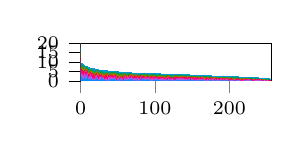
\begin{tikzpicture}

\definecolor{chocolate1961050}{RGB}{196,105,0}
\definecolor{crimson255078}{RGB}{255,0,78}
\definecolor{darkgray153}{RGB}{153,153,153}
\definecolor{darkslategray38}{RGB}{38,38,38}
\definecolor{darkslategray51}{RGB}{51,51,51}
\definecolor{darkturquoise0155207}{RGB}{0,155,207}
\definecolor{deeppink2510138}{RGB}{251,0,138}
\definecolor{dodgerblue0138250}{RGB}{0,138,250}
\definecolor{lightgray204}{RGB}{204,204,204}
\definecolor{mediumorchid21958191}{RGB}{219,58,191}
\definecolor{mediumpurple16495229}{RGB}{164,95,229}
\definecolor{olivedrab851440}{RGB}{85,144,0}
\definecolor{royalblue60122251}{RGB}{60,122,251}
\definecolor{teal015699}{RGB}{0,156,99}

\begin{axis}[
width=0.33\textwidth,
height=0.17\textwidth,
tick label style={font=\scriptsize},
tick align=outside,
tick pos=left,
xmin=0, xmax=256,
y grid style={darkgray176},
ymin=0, ymax=20,
ytick style={color=black},
ytick={0,5,10,15,20},
]
\addplot [semithick, darkgray153, forget plot]
table {%
0 4.44089209850063e-16
0 20
};
\draw[draw=none,fill=dodgerblue0138250] (axis cs:-0.35,0) rectangle (axis cs:0.35,4.24967489715146);

\draw[draw=none,fill=dodgerblue0138250] (axis cs:0.65,0) rectangle (axis cs:1.35,1.14147918921404);
\draw[draw=none,fill=dodgerblue0138250] (axis cs:1.65,0) rectangle (axis cs:2.35,0.709982915459545);
\draw[draw=none,fill=dodgerblue0138250] (axis cs:2.65,0) rectangle (axis cs:3.35,0.924662307117379);
\draw[draw=none,fill=dodgerblue0138250] (axis cs:3.65,0) rectangle (axis cs:4.35,0.654928242552686);
\draw[draw=none,fill=dodgerblue0138250] (axis cs:4.65,0) rectangle (axis cs:5.35,1.48750755909036);
\draw[draw=none,fill=dodgerblue0138250] (axis cs:5.65,0) rectangle (axis cs:6.35,0.565941043249339);
\draw[draw=none,fill=dodgerblue0138250] (axis cs:6.65,0) rectangle (axis cs:7.35,0.994689456756425);
\draw[draw=none,fill=dodgerblue0138250] (axis cs:7.65,0) rectangle (axis cs:8.35,1.00184580613186);
\draw[draw=none,fill=dodgerblue0138250] (axis cs:8.65,0) rectangle (axis cs:9.35,2.07389298738517);
\draw[draw=none,fill=dodgerblue0138250] (axis cs:9.65,0) rectangle (axis cs:10.35,0.522410824988771);
\draw[draw=none,fill=dodgerblue0138250] (axis cs:10.65,0) rectangle (axis cs:11.35,0.481421586718384);
\draw[draw=none,fill=dodgerblue0138250] (axis cs:11.65,0) rectangle (axis cs:12.35,0.557171120166251);
\draw[draw=none,fill=dodgerblue0138250] (axis cs:12.65,0) rectangle (axis cs:13.35,0.686737705346382);
\draw[draw=none,fill=dodgerblue0138250] (axis cs:13.65,0) rectangle (axis cs:14.35,0.789751059284547);
\draw[draw=none,fill=dodgerblue0138250] (axis cs:14.65,0) rectangle (axis cs:15.35,1.81951660681215);
\draw[draw=none,fill=dodgerblue0138250] (axis cs:15.65,0) rectangle (axis cs:16.35,0.639882056476918);
\draw[draw=none,fill=dodgerblue0138250] (axis cs:16.65,0) rectangle (axis cs:17.35,0.792515117949498);
\draw[draw=none,fill=dodgerblue0138250] (axis cs:17.65,0) rectangle (axis cs:18.35,0.350928572268253);
\draw[draw=none,fill=dodgerblue0138250] (axis cs:18.65,0) rectangle (axis cs:19.35,0.299287919344237);
\draw[draw=none,fill=dodgerblue0138250] (axis cs:19.65,0) rectangle (axis cs:20.35,0.502368755728914);
\draw[draw=none,fill=dodgerblue0138250] (axis cs:20.65,0) rectangle (axis cs:21.35,0.938147475064182);
\draw[draw=none,fill=dodgerblue0138250] (axis cs:21.65,0) rectangle (axis cs:22.35,0.60803640051253);
\draw[draw=none,fill=dodgerblue0138250] (axis cs:22.65,0) rectangle (axis cs:23.35,0.467265381449524);
\draw[draw=none,fill=dodgerblue0138250] (axis cs:23.65,0) rectangle (axis cs:24.35,0.209798611448114);
\draw[draw=none,fill=dodgerblue0138250] (axis cs:24.65,0) rectangle (axis cs:25.35,0.387877328342766);
\draw[draw=none,fill=dodgerblue0138250] (axis cs:25.65,0) rectangle (axis cs:26.35,1.02163846930525);
\draw[draw=none,fill=dodgerblue0138250] (axis cs:26.65,0) rectangle (axis cs:27.35,0.651219359308928);
\draw[draw=none,fill=dodgerblue0138250] (axis cs:27.65,0) rectangle (axis cs:28.35,1.1145483897076);
\draw[draw=none,fill=dodgerblue0138250] (axis cs:28.65,0) rectangle (axis cs:29.35,0.624032869751399);
\draw[draw=none,fill=dodgerblue0138250] (axis cs:29.65,0) rectangle (axis cs:30.35,1.0539413468533);
\draw[draw=none,fill=dodgerblue0138250] (axis cs:30.65,0) rectangle (axis cs:31.35,0.645184517761486);
\draw[draw=none,fill=dodgerblue0138250] (axis cs:31.65,0) rectangle (axis cs:32.35,0.402247215448603);
\draw[draw=none,fill=dodgerblue0138250] (axis cs:32.65,0) rectangle (axis cs:33.35,0.210389872615225);
\draw[draw=none,fill=dodgerblue0138250] (axis cs:33.65,0) rectangle (axis cs:34.35,0.437860844839137);
\draw[draw=none,fill=dodgerblue0138250] (axis cs:34.65,0) rectangle (axis cs:35.35,1.36325231847697);
\draw[draw=none,fill=dodgerblue0138250] (axis cs:35.65,0) rectangle (axis cs:36.35,0.152372532206355);
\draw[draw=none,fill=dodgerblue0138250] (axis cs:36.65,0) rectangle (axis cs:37.35,0.268513311664502);
\draw[draw=none,fill=dodgerblue0138250] (axis cs:37.65,0) rectangle (axis cs:38.35,0.191224835215737);
\draw[draw=none,fill=dodgerblue0138250] (axis cs:38.65,0) rectangle (axis cs:39.35,0.224802629635995);
\draw[draw=none,fill=dodgerblue0138250] (axis cs:39.65,0) rectangle (axis cs:40.35,0.532074888467099);
\draw[draw=none,fill=dodgerblue0138250] (axis cs:40.65,0) rectangle (axis cs:41.35,0.606089859851403);
\draw[draw=none,fill=dodgerblue0138250] (axis cs:41.65,0) rectangle (axis cs:42.35,0.566952733471645);
\draw[draw=none,fill=dodgerblue0138250] (axis cs:42.65,0) rectangle (axis cs:43.35,0.389507986976599);
\draw[draw=none,fill=dodgerblue0138250] (axis cs:43.65,0) rectangle (axis cs:44.35,0.652988907879699);
\draw[draw=none,fill=dodgerblue0138250] (axis cs:44.65,0) rectangle (axis cs:45.35,0.539566243686143);
\draw[draw=none,fill=dodgerblue0138250] (axis cs:45.65,0) rectangle (axis cs:46.35,0.369767622616746);
\draw[draw=none,fill=dodgerblue0138250] (axis cs:46.65,0) rectangle (axis cs:47.35,0.486887465139692);
\draw[draw=none,fill=dodgerblue0138250] (axis cs:47.65,0) rectangle (axis cs:48.35,0.278812916135399);
\draw[draw=none,fill=dodgerblue0138250] (axis cs:48.65,0) rectangle (axis cs:49.35,0.433008688501721);
\draw[draw=none,fill=dodgerblue0138250] (axis cs:49.65,0) rectangle (axis cs:50.35,0.612817466144042);
\draw[draw=none,fill=dodgerblue0138250] (axis cs:50.65,0) rectangle (axis cs:51.35,0.894917413102378);
\draw[draw=none,fill=dodgerblue0138250] (axis cs:51.65,0) rectangle (axis cs:52.35,0.133761955455482);
\draw[draw=none,fill=dodgerblue0138250] (axis cs:52.65,0) rectangle (axis cs:53.35,0.525743108916097);
\draw[draw=none,fill=dodgerblue0138250] (axis cs:53.65,0) rectangle (axis cs:54.35,0.495502838526907);
\draw[draw=none,fill=dodgerblue0138250] (axis cs:54.65,0) rectangle (axis cs:55.35,0.369989248904064);
\draw[draw=none,fill=dodgerblue0138250] (axis cs:55.65,0) rectangle (axis cs:56.35,0.502988108503461);
\draw[draw=none,fill=dodgerblue0138250] (axis cs:56.65,0) rectangle (axis cs:57.35,0.240020974519495);
\draw[draw=none,fill=dodgerblue0138250] (axis cs:57.65,0) rectangle (axis cs:58.35,0.189232384895155);
\draw[draw=none,fill=dodgerblue0138250] (axis cs:58.65,0) rectangle (axis cs:59.35,0.348850527553648);
\draw[draw=none,fill=dodgerblue0138250] (axis cs:59.65,0) rectangle (axis cs:60.35,0.41570759334382);
\draw[draw=none,fill=dodgerblue0138250] (axis cs:60.65,0) rectangle (axis cs:61.35,0.270877559056094);
\draw[draw=none,fill=dodgerblue0138250] (axis cs:61.65,0) rectangle (axis cs:62.35,0.716666583174643);
\draw[draw=none,fill=dodgerblue0138250] (axis cs:62.65,0) rectangle (axis cs:63.35,0.277568379246236);
\draw[draw=none,fill=dodgerblue0138250] (axis cs:63.65,0) rectangle (axis cs:64.35,0.446526851955253);
\draw[draw=none,fill=dodgerblue0138250] (axis cs:64.65,0) rectangle (axis cs:65.35,0.619087654976162);
\draw[draw=none,fill=dodgerblue0138250] (axis cs:65.65,0) rectangle (axis cs:66.35,0.282634023254709);
\draw[draw=none,fill=dodgerblue0138250] (axis cs:66.65,0) rectangle (axis cs:67.35,0.256518552468611);
\draw[draw=none,fill=dodgerblue0138250] (axis cs:67.65,0) rectangle (axis cs:68.35,0.638424633659961);
\draw[draw=none,fill=dodgerblue0138250] (axis cs:68.65,0) rectangle (axis cs:69.35,0.207775978373047);
\draw[draw=none,fill=dodgerblue0138250] (axis cs:69.65,0) rectangle (axis cs:70.35,0.506436552649802);
\draw[draw=none,fill=dodgerblue0138250] (axis cs:70.65,0) rectangle (axis cs:71.35,0.45563764417589);
\draw[draw=none,fill=dodgerblue0138250] (axis cs:71.65,0) rectangle (axis cs:72.35,0.216602210023325);
\draw[draw=none,fill=dodgerblue0138250] (axis cs:72.65,0) rectangle (axis cs:73.35,0.511726014152557);
\draw[draw=none,fill=dodgerblue0138250] (axis cs:73.65,0) rectangle (axis cs:74.35,0.332459025787859);
\draw[draw=none,fill=dodgerblue0138250] (axis cs:74.65,0) rectangle (axis cs:75.35,0.362708130570743);
\draw[draw=none,fill=dodgerblue0138250] (axis cs:75.65,0) rectangle (axis cs:76.35,0.707059498904953);
\draw[draw=none,fill=dodgerblue0138250] (axis cs:76.65,0) rectangle (axis cs:77.35,0.936003645635139);
\draw[draw=none,fill=dodgerblue0138250] (axis cs:77.65,0) rectangle (axis cs:78.35,0.238412289239029);
\draw[draw=none,fill=dodgerblue0138250] (axis cs:78.65,0) rectangle (axis cs:79.35,0.250404002429524);
\draw[draw=none,fill=dodgerblue0138250] (axis cs:79.65,0) rectangle (axis cs:80.35,0.851930673510598);
\draw[draw=none,fill=dodgerblue0138250] (axis cs:80.65,0) rectangle (axis cs:81.35,0.626936691911339);
\draw[draw=none,fill=dodgerblue0138250] (axis cs:81.65,0) rectangle (axis cs:82.35,0.378343615913005);
\draw[draw=none,fill=dodgerblue0138250] (axis cs:82.65,0) rectangle (axis cs:83.35,0.530182737484025);
\draw[draw=none,fill=dodgerblue0138250] (axis cs:83.65,0) rectangle (axis cs:84.35,0.276142320063086);
\draw[draw=none,fill=dodgerblue0138250] (axis cs:84.65,0) rectangle (axis cs:85.35,0.153717068874669);
\draw[draw=none,fill=dodgerblue0138250] (axis cs:85.65,0) rectangle (axis cs:86.35,0.569714732352906);
\draw[draw=none,fill=dodgerblue0138250] (axis cs:86.65,0) rectangle (axis cs:87.35,0.363386572926066);
\draw[draw=none,fill=dodgerblue0138250] (axis cs:87.65,0) rectangle (axis cs:88.35,0.866320949314817);
\draw[draw=none,fill=dodgerblue0138250] (axis cs:88.65,0) rectangle (axis cs:89.35,0.509872607735195);
\draw[draw=none,fill=dodgerblue0138250] (axis cs:89.65,0) rectangle (axis cs:90.35,1.01299356157787);
\draw[draw=none,fill=dodgerblue0138250] (axis cs:90.65,0) rectangle (axis cs:91.35,0.449383287377538);
\draw[draw=none,fill=dodgerblue0138250] (axis cs:91.65,0) rectangle (axis cs:92.35,0.565033058347222);
\draw[draw=none,fill=dodgerblue0138250] (axis cs:92.65,0) rectangle (axis cs:93.35,0.156849740248987);
\draw[draw=none,fill=dodgerblue0138250] (axis cs:93.65,0) rectangle (axis cs:94.35,0.490718138486441);
\draw[draw=none,fill=dodgerblue0138250] (axis cs:94.65,0) rectangle (axis cs:95.35,0.190529760883329);
\draw[draw=none,fill=dodgerblue0138250] (axis cs:95.65,0) rectangle (axis cs:96.35,1.08093623498871);
\draw[draw=none,fill=dodgerblue0138250] (axis cs:96.65,0) rectangle (axis cs:97.35,0.173352993284841);
\draw[draw=none,fill=dodgerblue0138250] (axis cs:97.65,0) rectangle (axis cs:98.35,0.238239435670047);
\draw[draw=none,fill=dodgerblue0138250] (axis cs:98.65,0) rectangle (axis cs:99.35,0.293282677175004);
\draw[draw=none,fill=dodgerblue0138250] (axis cs:99.65,0) rectangle (axis cs:100.35,0.507632461256643);
\draw[draw=none,fill=dodgerblue0138250] (axis cs:100.65,0) rectangle (axis cs:101.35,0.647731077858594);
\draw[draw=none,fill=dodgerblue0138250] (axis cs:101.65,0) rectangle (axis cs:102.35,0.412836726446898);
\draw[draw=none,fill=dodgerblue0138250] (axis cs:102.65,0) rectangle (axis cs:103.35,0.595368129620567);
\draw[draw=none,fill=dodgerblue0138250] (axis cs:103.65,0) rectangle (axis cs:104.35,0.216377146043026);
\draw[draw=none,fill=dodgerblue0138250] (axis cs:104.65,0) rectangle (axis cs:105.35,0.592075033496238);
\draw[draw=none,fill=dodgerblue0138250] (axis cs:105.65,0) rectangle (axis cs:106.35,0.259145250885383);
\draw[draw=none,fill=dodgerblue0138250] (axis cs:106.65,0) rectangle (axis cs:107.35,0.335162643662081);
\draw[draw=none,fill=dodgerblue0138250] (axis cs:107.65,0) rectangle (axis cs:108.35,0.295889150211062);
\draw[draw=none,fill=dodgerblue0138250] (axis cs:108.65,0) rectangle (axis cs:109.35,0.360030468557123);
\draw[draw=none,fill=dodgerblue0138250] (axis cs:109.65,0) rectangle (axis cs:110.35,0.203378407118876);
\draw[draw=none,fill=dodgerblue0138250] (axis cs:110.65,0) rectangle (axis cs:111.35,0.29743739502175);
\draw[draw=none,fill=dodgerblue0138250] (axis cs:111.65,0) rectangle (axis cs:112.35,0.457752891391476);
\draw[draw=none,fill=dodgerblue0138250] (axis cs:112.65,0) rectangle (axis cs:113.35,0.266046482443856);
\draw[draw=none,fill=dodgerblue0138250] (axis cs:113.65,0) rectangle (axis cs:114.35,0.451891773475972);
\draw[draw=none,fill=dodgerblue0138250] (axis cs:114.65,0) rectangle (axis cs:115.35,0.193732417829949);
\draw[draw=none,fill=dodgerblue0138250] (axis cs:115.65,0) rectangle (axis cs:116.35,0.162768641381446);
\draw[draw=none,fill=dodgerblue0138250] (axis cs:116.65,0) rectangle (axis cs:117.35,0.26040244754442);
\draw[draw=none,fill=dodgerblue0138250] (axis cs:117.65,0) rectangle (axis cs:118.35,0.224440422416869);
\draw[draw=none,fill=dodgerblue0138250] (axis cs:118.65,0) rectangle (axis cs:119.35,0.282404066308733);
\draw[draw=none,fill=dodgerblue0138250] (axis cs:119.65,0) rectangle (axis cs:120.35,0.230378005741292);
\draw[draw=none,fill=dodgerblue0138250] (axis cs:120.65,0) rectangle (axis cs:121.35,0.240228207313646);
\draw[draw=none,fill=dodgerblue0138250] (axis cs:121.65,0) rectangle (axis cs:122.35,0.41364933596469);
\draw[draw=none,fill=dodgerblue0138250] (axis cs:122.65,0) rectangle (axis cs:123.35,0.178886132487222);
\draw[draw=none,fill=dodgerblue0138250] (axis cs:123.65,0) rectangle (axis cs:124.35,0.176790467081492);
\draw[draw=none,fill=dodgerblue0138250] (axis cs:124.65,0) rectangle (axis cs:125.35,0.156143573686564);
\draw[draw=none,fill=dodgerblue0138250] (axis cs:125.65,0) rectangle (axis cs:126.35,0.228580553728725);
\draw[draw=none,fill=dodgerblue0138250] (axis cs:126.65,0) rectangle (axis cs:127.35,0.180370905605832);
\draw[draw=none,fill=dodgerblue0138250] (axis cs:127.65,0) rectangle (axis cs:128.35,0.769850312693865);
\draw[draw=none,fill=dodgerblue0138250] (axis cs:128.65,0) rectangle (axis cs:129.35,0.147891533812443);
\draw[draw=none,fill=dodgerblue0138250] (axis cs:129.65,0) rectangle (axis cs:130.35,0.326937044244459);
\draw[draw=none,fill=dodgerblue0138250] (axis cs:130.65,0) rectangle (axis cs:131.35,0.206456021207313);
\draw[draw=none,fill=dodgerblue0138250] (axis cs:131.65,0) rectangle (axis cs:132.35,0.128835252480565);
\draw[draw=none,fill=dodgerblue0138250] (axis cs:132.65,0) rectangle (axis cs:133.35,0.431991425572096);
\draw[draw=none,fill=dodgerblue0138250] (axis cs:133.65,0) rectangle (axis cs:134.35,0.299614890661194);
\draw[draw=none,fill=dodgerblue0138250] (axis cs:134.65,0) rectangle (axis cs:135.35,0.229841005109973);
\draw[draw=none,fill=dodgerblue0138250] (axis cs:135.65,0) rectangle (axis cs:136.35,0.263660810568251);
\draw[draw=none,fill=dodgerblue0138250] (axis cs:136.65,0) rectangle (axis cs:137.35,0.34987641797496);
\draw[draw=none,fill=dodgerblue0138250] (axis cs:137.65,0) rectangle (axis cs:138.35,0.446449305325845);
\draw[draw=none,fill=dodgerblue0138250] (axis cs:138.65,0) rectangle (axis cs:139.35,0.552203504691202);
\draw[draw=none,fill=dodgerblue0138250] (axis cs:139.65,0) rectangle (axis cs:140.35,0.451230142103634);
\draw[draw=none,fill=dodgerblue0138250] (axis cs:140.65,0) rectangle (axis cs:141.35,0.27902496772071);
\draw[draw=none,fill=dodgerblue0138250] (axis cs:141.65,0) rectangle (axis cs:142.35,0.098630310445696);
\draw[draw=none,fill=dodgerblue0138250] (axis cs:142.65,0) rectangle (axis cs:143.35,0.42322489498227);
\draw[draw=none,fill=dodgerblue0138250] (axis cs:143.65,0) rectangle (axis cs:144.35,0.112084583333221);
\draw[draw=none,fill=dodgerblue0138250] (axis cs:144.65,0) rectangle (axis cs:145.35,0.353544048277723);
\draw[draw=none,fill=dodgerblue0138250] (axis cs:145.65,0) rectangle (axis cs:146.35,0.472249232634163);
\draw[draw=none,fill=dodgerblue0138250] (axis cs:146.65,0) rectangle (axis cs:147.35,0.397877636445601);
\draw[draw=none,fill=dodgerblue0138250] (axis cs:147.65,0) rectangle (axis cs:148.35,0.0875579608210284);
\draw[draw=none,fill=dodgerblue0138250] (axis cs:148.65,0) rectangle (axis cs:149.35,0.313747401128926);
\draw[draw=none,fill=dodgerblue0138250] (axis cs:149.65,0) rectangle (axis cs:150.35,0.16284788567332);
\draw[draw=none,fill=dodgerblue0138250] (axis cs:150.65,0) rectangle (axis cs:151.35,0.364045518499362);
\draw[draw=none,fill=dodgerblue0138250] (axis cs:151.65,0) rectangle (axis cs:152.35,0.366650471183634);
\draw[draw=none,fill=dodgerblue0138250] (axis cs:152.65,0) rectangle (axis cs:153.35,0.359730604512476);
\draw[draw=none,fill=dodgerblue0138250] (axis cs:153.65,0) rectangle (axis cs:154.35,0.380497160809067);
\draw[draw=none,fill=dodgerblue0138250] (axis cs:154.65,0) rectangle (axis cs:155.35,0.543075125890836);
\draw[draw=none,fill=dodgerblue0138250] (axis cs:155.65,0) rectangle (axis cs:156.35,0.135594267652768);
\draw[draw=none,fill=dodgerblue0138250] (axis cs:156.65,0) rectangle (axis cs:157.35,0.188231901850106);
\draw[draw=none,fill=dodgerblue0138250] (axis cs:157.65,0) rectangle (axis cs:158.35,0.208980285430433);
\draw[draw=none,fill=dodgerblue0138250] (axis cs:158.65,0) rectangle (axis cs:159.35,0.250040923696894);
\draw[draw=none,fill=dodgerblue0138250] (axis cs:159.65,0) rectangle (axis cs:160.35,0.5606502514548);
\draw[draw=none,fill=dodgerblue0138250] (axis cs:160.65,0) rectangle (axis cs:161.35,0.145420274050645);
\draw[draw=none,fill=dodgerblue0138250] (axis cs:161.65,0) rectangle (axis cs:162.35,0.36984404702696);
\draw[draw=none,fill=dodgerblue0138250] (axis cs:162.65,0) rectangle (axis cs:163.35,0.223870616665411);
\draw[draw=none,fill=dodgerblue0138250] (axis cs:163.65,0) rectangle (axis cs:164.35,0.0942834391632661);
\draw[draw=none,fill=dodgerblue0138250] (axis cs:164.65,0) rectangle (axis cs:165.35,1.00540600886803);
\draw[draw=none,fill=dodgerblue0138250] (axis cs:165.65,0) rectangle (axis cs:166.35,0.37099679221015);
\draw[draw=none,fill=dodgerblue0138250] (axis cs:166.65,0) rectangle (axis cs:167.35,0.443171826702918);
\draw[draw=none,fill=dodgerblue0138250] (axis cs:167.65,0) rectangle (axis cs:168.35,0.121501396986583);
\draw[draw=none,fill=dodgerblue0138250] (axis cs:168.65,0) rectangle (axis cs:169.35,0.222121921800257);
\draw[draw=none,fill=dodgerblue0138250] (axis cs:169.65,0) rectangle (axis cs:170.35,0.247201151463937);
\draw[draw=none,fill=dodgerblue0138250] (axis cs:170.65,0) rectangle (axis cs:171.35,0.13571951951714);
\draw[draw=none,fill=dodgerblue0138250] (axis cs:171.65,0) rectangle (axis cs:172.35,0.206468949641099);
\draw[draw=none,fill=dodgerblue0138250] (axis cs:172.65,0) rectangle (axis cs:173.35,0.170619896044005);
\draw[draw=none,fill=dodgerblue0138250] (axis cs:173.65,0) rectangle (axis cs:174.35,0.108758179594664);
\draw[draw=none,fill=dodgerblue0138250] (axis cs:174.65,0) rectangle (axis cs:175.35,0.200101832007278);
\draw[draw=none,fill=dodgerblue0138250] (axis cs:175.65,0) rectangle (axis cs:176.35,0.20242851919786);
\draw[draw=none,fill=dodgerblue0138250] (axis cs:176.65,0) rectangle (axis cs:177.35,0.0822015913718393);
\draw[draw=none,fill=dodgerblue0138250] (axis cs:177.65,0) rectangle (axis cs:178.35,0.384275102848372);
\draw[draw=none,fill=dodgerblue0138250] (axis cs:178.65,0) rectangle (axis cs:179.35,0.45703745717816);
\draw[draw=none,fill=dodgerblue0138250] (axis cs:179.65,0) rectangle (axis cs:180.35,0.285791225655969);
\draw[draw=none,fill=dodgerblue0138250] (axis cs:180.65,0) rectangle (axis cs:181.35,0.332291237215925);
\draw[draw=none,fill=dodgerblue0138250] (axis cs:181.65,0) rectangle (axis cs:182.35,0.286844574863007);
\draw[draw=none,fill=dodgerblue0138250] (axis cs:182.65,0) rectangle (axis cs:183.35,0.160264374035429);
\draw[draw=none,fill=dodgerblue0138250] (axis cs:183.65,0) rectangle (axis cs:184.35,0.357239002972534);
\draw[draw=none,fill=dodgerblue0138250] (axis cs:184.65,0) rectangle (axis cs:185.35,0.204006682837673);
\draw[draw=none,fill=dodgerblue0138250] (axis cs:185.65,0) rectangle (axis cs:186.35,0.163553654538562);
\draw[draw=none,fill=dodgerblue0138250] (axis cs:186.65,0) rectangle (axis cs:187.35,0.111508635275954);
\draw[draw=none,fill=dodgerblue0138250] (axis cs:187.65,0) rectangle (axis cs:188.35,0.126485255004111);
\draw[draw=none,fill=dodgerblue0138250] (axis cs:188.65,0) rectangle (axis cs:189.35,0.53697890400388);
\draw[draw=none,fill=dodgerblue0138250] (axis cs:189.65,0) rectangle (axis cs:190.35,0.229393348761258);
\draw[draw=none,fill=dodgerblue0138250] (axis cs:190.65,0) rectangle (axis cs:191.35,0.290689122457733);
\draw[draw=none,fill=dodgerblue0138250] (axis cs:191.65,0) rectangle (axis cs:192.35,0.227994857999285);
\draw[draw=none,fill=dodgerblue0138250] (axis cs:192.65,0) rectangle (axis cs:193.35,0.20518204619475);
\draw[draw=none,fill=dodgerblue0138250] (axis cs:193.65,0) rectangle (axis cs:194.35,0.338329968685836);
\draw[draw=none,fill=dodgerblue0138250] (axis cs:194.65,0) rectangle (axis cs:195.35,0.236465937718869);
\draw[draw=none,fill=dodgerblue0138250] (axis cs:195.65,0) rectangle (axis cs:196.35,0.158850933590155);
\draw[draw=none,fill=dodgerblue0138250] (axis cs:196.65,0) rectangle (axis cs:197.35,0.349058198323323);
\draw[draw=none,fill=dodgerblue0138250] (axis cs:197.65,0) rectangle (axis cs:198.35,0.223605216349579);
\draw[draw=none,fill=dodgerblue0138250] (axis cs:198.65,0) rectangle (axis cs:199.35,0.272414966541801);
\draw[draw=none,fill=dodgerblue0138250] (axis cs:199.65,0) rectangle (axis cs:200.35,0.202496700215306);
\draw[draw=none,fill=dodgerblue0138250] (axis cs:200.65,0) rectangle (axis cs:201.35,0.226759634201741);
\draw[draw=none,fill=dodgerblue0138250] (axis cs:201.65,0) rectangle (axis cs:202.35,0.114387681119451);
\draw[draw=none,fill=dodgerblue0138250] (axis cs:202.65,0) rectangle (axis cs:203.35,0.235459818096766);
\draw[draw=none,fill=dodgerblue0138250] (axis cs:203.65,0) rectangle (axis cs:204.35,0.315160016689246);
\draw[draw=none,fill=dodgerblue0138250] (axis cs:204.65,0) rectangle (axis cs:205.35,0.172811004800357);
\draw[draw=none,fill=dodgerblue0138250] (axis cs:205.65,0) rectangle (axis cs:206.35,0.140183736698464);
\draw[draw=none,fill=dodgerblue0138250] (axis cs:206.65,0) rectangle (axis cs:207.35,0.113898682387762);
\draw[draw=none,fill=dodgerblue0138250] (axis cs:207.65,0) rectangle (axis cs:208.35,0.357955849427777);
\draw[draw=none,fill=dodgerblue0138250] (axis cs:208.65,0) rectangle (axis cs:209.35,0.371314720196738);
\draw[draw=none,fill=dodgerblue0138250] (axis cs:209.65,0) rectangle (axis cs:210.35,0.0970605494018972);
\draw[draw=none,fill=dodgerblue0138250] (axis cs:210.65,0) rectangle (axis cs:211.35,0.257504971041109);
\draw[draw=none,fill=dodgerblue0138250] (axis cs:211.65,0) rectangle (axis cs:212.35,0.223961687089903);
\draw[draw=none,fill=dodgerblue0138250] (axis cs:212.65,0) rectangle (axis cs:213.35,0.217030431487558);
\draw[draw=none,fill=dodgerblue0138250] (axis cs:213.65,0) rectangle (axis cs:214.35,0.39984511952949);
\draw[draw=none,fill=dodgerblue0138250] (axis cs:214.65,0) rectangle (axis cs:215.35,0.0668638916914855);
\draw[draw=none,fill=dodgerblue0138250] (axis cs:215.65,0) rectangle (axis cs:216.35,0.155994849784785);
\draw[draw=none,fill=dodgerblue0138250] (axis cs:216.65,0) rectangle (axis cs:217.35,0.123248318140418);
\draw[draw=none,fill=dodgerblue0138250] (axis cs:217.65,0) rectangle (axis cs:218.35,0.362563243469914);
\draw[draw=none,fill=dodgerblue0138250] (axis cs:218.65,0) rectangle (axis cs:219.35,0.141328154901771);
\draw[draw=none,fill=dodgerblue0138250] (axis cs:219.65,0) rectangle (axis cs:220.35,0.202623158540537);
\draw[draw=none,fill=dodgerblue0138250] (axis cs:220.65,0) rectangle (axis cs:221.35,0.149090068231378);
\draw[draw=none,fill=dodgerblue0138250] (axis cs:221.65,0) rectangle (axis cs:222.35,0.231553088497113);
\draw[draw=none,fill=dodgerblue0138250] (axis cs:222.65,0) rectangle (axis cs:223.35,0.133689866770785);
\draw[draw=none,fill=dodgerblue0138250] (axis cs:223.65,0) rectangle (axis cs:224.35,0.0764951952369022);
\draw[draw=none,fill=dodgerblue0138250] (axis cs:224.65,0) rectangle (axis cs:225.35,0.240645013099805);
\draw[draw=none,fill=dodgerblue0138250] (axis cs:225.65,0) rectangle (axis cs:226.35,0.303049936514569);
\draw[draw=none,fill=dodgerblue0138250] (axis cs:226.65,0) rectangle (axis cs:227.35,0.260026128717644);
\draw[draw=none,fill=dodgerblue0138250] (axis cs:227.65,0) rectangle (axis cs:228.35,0.144286600769255);
\draw[draw=none,fill=dodgerblue0138250] (axis cs:228.65,0) rectangle (axis cs:229.35,0.163967169099773);
\draw[draw=none,fill=dodgerblue0138250] (axis cs:229.65,0) rectangle (axis cs:230.35,0.186876364324843);
\draw[draw=none,fill=dodgerblue0138250] (axis cs:230.65,0) rectangle (axis cs:231.35,0.0783451911508018);
\draw[draw=none,fill=dodgerblue0138250] (axis cs:231.65,0) rectangle (axis cs:232.35,0.103385853325911);
\draw[draw=none,fill=dodgerblue0138250] (axis cs:232.65,0) rectangle (axis cs:233.35,0.132734977516754);
\draw[draw=none,fill=dodgerblue0138250] (axis cs:233.65,0) rectangle (axis cs:234.35,0.167079606807576);
\draw[draw=none,fill=dodgerblue0138250] (axis cs:234.65,0) rectangle (axis cs:235.35,0.0993656748401106);
\draw[draw=none,fill=dodgerblue0138250] (axis cs:235.65,0) rectangle (axis cs:236.35,0.100900751763204);
\draw[draw=none,fill=dodgerblue0138250] (axis cs:236.65,0) rectangle (axis cs:237.35,0.10775140052115);
\draw[draw=none,fill=dodgerblue0138250] (axis cs:237.65,0) rectangle (axis cs:238.35,0.178194902877165);
\draw[draw=none,fill=dodgerblue0138250] (axis cs:238.65,0) rectangle (axis cs:239.35,0.305416283649354);
\draw[draw=none,fill=dodgerblue0138250] (axis cs:239.65,0) rectangle (axis cs:240.35,0.12146540526457);
\draw[draw=none,fill=dodgerblue0138250] (axis cs:240.65,0) rectangle (axis cs:241.35,0.359772275965005);
\draw[draw=none,fill=dodgerblue0138250] (axis cs:241.65,0) rectangle (axis cs:242.35,0.322049255935353);
\draw[draw=none,fill=dodgerblue0138250] (axis cs:242.65,0) rectangle (axis cs:243.35,0.188069511396169);
\draw[draw=none,fill=dodgerblue0138250] (axis cs:243.65,0) rectangle (axis cs:244.35,0.134127134700457);
\draw[draw=none,fill=dodgerblue0138250] (axis cs:244.65,0) rectangle (axis cs:245.35,0.26340379889305);
\draw[draw=none,fill=dodgerblue0138250] (axis cs:245.65,0) rectangle (axis cs:246.35,0.0895143812547981);
\draw[draw=none,fill=dodgerblue0138250] (axis cs:246.65,0) rectangle (axis cs:247.35,0.164302536036241);
\draw[draw=none,fill=dodgerblue0138250] (axis cs:247.65,0) rectangle (axis cs:248.35,0.108629697096786);
\draw[draw=none,fill=dodgerblue0138250] (axis cs:248.65,0) rectangle (axis cs:249.35,0.0908596818854089);
\draw[draw=none,fill=dodgerblue0138250] (axis cs:249.65,0) rectangle (axis cs:250.35,0.105246893142151);
\draw[draw=none,fill=dodgerblue0138250] (axis cs:250.65,0) rectangle (axis cs:251.35,0.293388077001169);
\draw[draw=none,fill=dodgerblue0138250] (axis cs:251.65,0) rectangle (axis cs:252.35,0.0865285631867617);
\draw[draw=none,fill=dodgerblue0138250] (axis cs:252.65,0) rectangle (axis cs:253.35,0.105918955441629);
\draw[draw=none,fill=dodgerblue0138250] (axis cs:253.65,0) rectangle (axis cs:254.35,0.127729778846092);
\draw[draw=none,fill=dodgerblue0138250] (axis cs:254.65,0) rectangle (axis cs:255.35,0.183123323244248);
\draw[draw=none,fill=royalblue60122251] (axis cs:-0.35,4.24967489715146) rectangle (axis cs:0.35,5.3773229946483);

\draw[draw=none,fill=royalblue60122251] (axis cs:0.65,1.14147918921404) rectangle (axis cs:1.35,2.13715557722538);
\draw[draw=none,fill=royalblue60122251] (axis cs:1.65,0.709982915459545) rectangle (axis cs:2.35,1.62727582113403);
\draw[draw=none,fill=royalblue60122251] (axis cs:2.65,0.924662307117379) rectangle (axis cs:3.35,2.49636773871069);
\draw[draw=none,fill=royalblue60122251] (axis cs:3.65,0.654928242552686) rectangle (axis cs:4.35,0.931419127896287);
\draw[draw=none,fill=royalblue60122251] (axis cs:4.65,1.48750755909036) rectangle (axis cs:5.35,2.32175712594249);
\draw[draw=none,fill=royalblue60122251] (axis cs:5.65,0.565941043249339) rectangle (axis cs:6.35,1.27421431203597);
\draw[draw=none,fill=royalblue60122251] (axis cs:6.65,0.994689456756425) rectangle (axis cs:7.35,1.89650386667351);
\draw[draw=none,fill=royalblue60122251] (axis cs:7.65,1.00184580613186) rectangle (axis cs:8.35,1.54737109353241);
\draw[draw=none,fill=royalblue60122251] (axis cs:8.65,2.07389298738517) rectangle (axis cs:9.35,2.95019558680523);
\draw[draw=none,fill=royalblue60122251] (axis cs:9.65,0.522410824988771) rectangle (axis cs:10.35,0.801177063086726);
\draw[draw=none,fill=royalblue60122251] (axis cs:10.65,0.481421586718384) rectangle (axis cs:11.35,0.952605558158833);
\draw[draw=none,fill=royalblue60122251] (axis cs:11.65,0.557171120166251) rectangle (axis cs:12.35,1.19378753581232);
\draw[draw=none,fill=royalblue60122251] (axis cs:12.65,0.686737705346382) rectangle (axis cs:13.35,1.79548219251076);
\draw[draw=none,fill=royalblue60122251] (axis cs:13.65,0.789751059284547) rectangle (axis cs:14.35,1.14185874607036);
\draw[draw=none,fill=royalblue60122251] (axis cs:14.65,1.81951660681215) rectangle (axis cs:15.35,1.92124847851423);
\draw[draw=none,fill=royalblue60122251] (axis cs:15.65,0.639882056476918) rectangle (axis cs:16.35,0.922875250832809);
\draw[draw=none,fill=royalblue60122251] (axis cs:16.65,0.792515117949498) rectangle (axis cs:17.35,1.1052913386994);
\draw[draw=none,fill=royalblue60122251] (axis cs:17.65,0.350928572268253) rectangle (axis cs:18.35,0.739654688719372);
\draw[draw=none,fill=royalblue60122251] (axis cs:18.65,0.299287919344237) rectangle (axis cs:19.35,0.895857649449062);
\draw[draw=none,fill=royalblue60122251] (axis cs:19.65,0.502368755728914) rectangle (axis cs:20.35,1.11557650288225);
\draw[draw=none,fill=royalblue60122251] (axis cs:20.65,0.938147475064182) rectangle (axis cs:21.35,2.21418542256735);
\draw[draw=none,fill=royalblue60122251] (axis cs:21.65,0.60803640051253) rectangle (axis cs:22.35,1.47627400848481);
\draw[draw=none,fill=royalblue60122251] (axis cs:22.65,0.467265381449524) rectangle (axis cs:23.35,0.774875616639366);
\draw[draw=none,fill=royalblue60122251] (axis cs:23.65,0.209798611448114) rectangle (axis cs:24.35,0.733840489042157);
\draw[draw=none,fill=royalblue60122251] (axis cs:24.65,0.387877328342766) rectangle (axis cs:25.35,0.741679100506346);
\draw[draw=none,fill=royalblue60122251] (axis cs:25.65,1.02163846930525) rectangle (axis cs:26.35,1.37587699080685);
\draw[draw=none,fill=royalblue60122251] (axis cs:26.65,0.651219359308928) rectangle (axis cs:27.35,0.871789916029472);
\draw[draw=none,fill=royalblue60122251] (axis cs:27.65,1.1145483897076) rectangle (axis cs:28.35,2.18657065495669);
\draw[draw=none,fill=royalblue60122251] (axis cs:28.65,0.624032869751399) rectangle (axis cs:29.35,1.73570578856851);
\draw[draw=none,fill=royalblue60122251] (axis cs:29.65,1.0539413468533) rectangle (axis cs:30.35,1.17726011479298);
\draw[draw=none,fill=royalblue60122251] (axis cs:30.65,0.645184517761486) rectangle (axis cs:31.35,1.51025875299156);
\draw[draw=none,fill=royalblue60122251] (axis cs:31.65,0.402247215448603) rectangle (axis cs:32.35,0.800557535998956);
\draw[draw=none,fill=royalblue60122251] (axis cs:32.65,0.210389872615225) rectangle (axis cs:33.35,0.468666282800244);
\draw[draw=none,fill=royalblue60122251] (axis cs:33.65,0.437860844839137) rectangle (axis cs:34.35,0.705466449414744);
\draw[draw=none,fill=royalblue60122251] (axis cs:34.65,1.36325231847697) rectangle (axis cs:35.35,1.9920029179663);
\draw[draw=none,fill=royalblue60122251] (axis cs:35.65,0.152372532206355) rectangle (axis cs:36.35,0.531890737987812);
\draw[draw=none,fill=royalblue60122251] (axis cs:36.65,0.268513311664502) rectangle (axis cs:37.35,0.365897271921887);
\draw[draw=none,fill=royalblue60122251] (axis cs:37.65,0.191224835215737) rectangle (axis cs:38.35,0.524546189944128);
\draw[draw=none,fill=royalblue60122251] (axis cs:38.65,0.224802629635995) rectangle (axis cs:39.35,0.78555112972012);
\draw[draw=none,fill=royalblue60122251] (axis cs:39.65,0.532074888467099) rectangle (axis cs:40.35,1.04932454873833);
\draw[draw=none,fill=royalblue60122251] (axis cs:40.65,0.606089859851403) rectangle (axis cs:41.35,0.927022583739782);
\draw[draw=none,fill=royalblue60122251] (axis cs:41.65,0.566952733471645) rectangle (axis cs:42.35,1.86091349347822);
\draw[draw=none,fill=royalblue60122251] (axis cs:42.65,0.389507986976599) rectangle (axis cs:43.35,1.17843703513963);
\draw[draw=none,fill=royalblue60122251] (axis cs:43.65,0.652988907879699) rectangle (axis cs:44.35,1.5274377231305);
\draw[draw=none,fill=royalblue60122251] (axis cs:44.65,0.539566243686143) rectangle (axis cs:45.35,1.13411455703972);
\draw[draw=none,fill=royalblue60122251] (axis cs:45.65,0.369767622616746) rectangle (axis cs:46.35,1.75651994625115);
\draw[draw=none,fill=royalblue60122251] (axis cs:46.65,0.486887465139692) rectangle (axis cs:47.35,1.52197126431247);
\draw[draw=none,fill=royalblue60122251] (axis cs:47.65,0.278812916135399) rectangle (axis cs:48.35,0.614416176161051);
\draw[draw=none,fill=royalblue60122251] (axis cs:48.65,0.433008688501721) rectangle (axis cs:49.35,0.752341512001579);
\draw[draw=none,fill=royalblue60122251] (axis cs:49.65,0.612817466144042) rectangle (axis cs:50.35,1.2113375235448);
\draw[draw=none,fill=royalblue60122251] (axis cs:50.65,0.894917413102378) rectangle (axis cs:51.35,1.4971808109422);
\draw[draw=none,fill=royalblue60122251] (axis cs:51.65,0.133761955455482) rectangle (axis cs:52.35,0.581751518756784);
\draw[draw=none,fill=royalblue60122251] (axis cs:52.65,0.525743108916097) rectangle (axis cs:53.35,0.944544691667921);
\draw[draw=none,fill=royalblue60122251] (axis cs:53.65,0.495502838526907) rectangle (axis cs:54.35,1.16468092828223);
\draw[draw=none,fill=royalblue60122251] (axis cs:54.65,0.369989248904064) rectangle (axis cs:55.35,0.682014754679687);
\draw[draw=none,fill=royalblue60122251] (axis cs:55.65,0.502988108503461) rectangle (axis cs:56.35,1.06989921307883);
\draw[draw=none,fill=royalblue60122251] (axis cs:56.65,0.240020974519495) rectangle (axis cs:57.35,0.350247552457888);
\draw[draw=none,fill=royalblue60122251] (axis cs:57.65,0.189232384895155) rectangle (axis cs:58.35,0.811572066522171);
\draw[draw=none,fill=royalblue60122251] (axis cs:58.65,0.348850527553648) rectangle (axis cs:59.35,0.561060361728093);
\draw[draw=none,fill=royalblue60122251] (axis cs:59.65,0.41570759334382) rectangle (axis cs:60.35,1.04994661858553);
\draw[draw=none,fill=royalblue60122251] (axis cs:60.65,0.270877559056094) rectangle (axis cs:61.35,0.971383359474536);
\draw[draw=none,fill=royalblue60122251] (axis cs:61.65,0.716666583174643) rectangle (axis cs:62.35,0.822483153463841);
\draw[draw=none,fill=royalblue60122251] (axis cs:62.65,0.277568379246236) rectangle (axis cs:63.35,0.404920288639018);
\draw[draw=none,fill=royalblue60122251] (axis cs:63.65,0.446526851955253) rectangle (axis cs:64.35,1.13045505904254);
\draw[draw=none,fill=royalblue60122251] (axis cs:64.65,0.619087654976162) rectangle (axis cs:65.35,0.726958829221);
\draw[draw=none,fill=royalblue60122251] (axis cs:65.65,0.282634023254709) rectangle (axis cs:66.35,0.587609654189974);
\draw[draw=none,fill=royalblue60122251] (axis cs:66.65,0.256518552468611) rectangle (axis cs:67.35,1.22712764942442);
\draw[draw=none,fill=royalblue60122251] (axis cs:67.65,0.638424633659961) rectangle (axis cs:68.35,1.48438137528918);
\draw[draw=none,fill=royalblue60122251] (axis cs:68.65,0.207775978373047) rectangle (axis cs:69.35,0.979824481039097);
\draw[draw=none,fill=royalblue60122251] (axis cs:69.65,0.506436552649802) rectangle (axis cs:70.35,1.40318147829145);
\draw[draw=none,fill=royalblue60122251] (axis cs:70.65,0.45563764417589) rectangle (axis cs:71.35,0.617614624456785);
\draw[draw=none,fill=royalblue60122251] (axis cs:71.65,0.216602210023325) rectangle (axis cs:72.35,0.30156999634019);
\draw[draw=none,fill=royalblue60122251] (axis cs:72.65,0.511726014152557) rectangle (axis cs:73.35,0.805702319937614);
\draw[draw=none,fill=royalblue60122251] (axis cs:73.65,0.332459025787859) rectangle (axis cs:74.35,0.438163330910548);
\draw[draw=none,fill=royalblue60122251] (axis cs:74.65,0.362708130570743) rectangle (axis cs:75.35,0.555506111790121);
\draw[draw=none,fill=royalblue60122251] (axis cs:75.65,0.707059498904953) rectangle (axis cs:76.35,1.44072526348927);
\draw[draw=none,fill=royalblue60122251] (axis cs:76.65,0.936003645635139) rectangle (axis cs:77.35,1.30436940959605);
\draw[draw=none,fill=royalblue60122251] (axis cs:77.65,0.238412289239029) rectangle (axis cs:78.35,0.386054647592646);
\draw[draw=none,fill=royalblue60122251] (axis cs:78.65,0.250404002429524) rectangle (axis cs:79.35,0.38714857497166);
\draw[draw=none,fill=royalblue60122251] (axis cs:79.65,0.851930673510598) rectangle (axis cs:80.35,1.76081999391516);
\draw[draw=none,fill=royalblue60122251] (axis cs:80.65,0.626936691911339) rectangle (axis cs:81.35,1.14937460348067);
\draw[draw=none,fill=royalblue60122251] (axis cs:81.65,0.378343615913005) rectangle (axis cs:82.35,0.618916366469181);
\draw[draw=none,fill=royalblue60122251] (axis cs:82.65,0.530182737484025) rectangle (axis cs:83.35,0.850975977766157);
\draw[draw=none,fill=royalblue60122251] (axis cs:83.65,0.276142320063086) rectangle (axis cs:84.35,1.25460352748633);
\draw[draw=none,fill=royalblue60122251] (axis cs:84.65,0.153717068874669) rectangle (axis cs:85.35,0.253993163634063);
\draw[draw=none,fill=royalblue60122251] (axis cs:85.65,0.569714732352906) rectangle (axis cs:86.35,1.20692896134104);
\draw[draw=none,fill=royalblue60122251] (axis cs:86.65,0.363386572926066) rectangle (axis cs:87.35,0.954438538789932);
\draw[draw=none,fill=royalblue60122251] (axis cs:87.65,0.866320949314817) rectangle (axis cs:88.35,1.02912941580383);
\draw[draw=none,fill=royalblue60122251] (axis cs:88.65,0.509872607735195) rectangle (axis cs:89.35,1.20777750652256);
\draw[draw=none,fill=royalblue60122251] (axis cs:89.65,1.01299356157787) rectangle (axis cs:90.35,1.32546605532902);
\draw[draw=none,fill=royalblue60122251] (axis cs:90.65,0.449383287377538) rectangle (axis cs:91.35,0.819741417483773);
\draw[draw=none,fill=royalblue60122251] (axis cs:91.65,0.565033058347222) rectangle (axis cs:92.35,0.718303662063299);
\draw[draw=none,fill=royalblue60122251] (axis cs:92.65,0.156849740248987) rectangle (axis cs:93.35,0.233354526988825);
\draw[draw=none,fill=royalblue60122251] (axis cs:93.65,0.490718138486441) rectangle (axis cs:94.35,0.816014412027587);
\draw[draw=none,fill=royalblue60122251] (axis cs:94.65,0.190529760883329) rectangle (axis cs:95.35,0.545520559375768);
\draw[draw=none,fill=royalblue60122251] (axis cs:95.65,1.08093623498871) rectangle (axis cs:96.35,1.68364323577588);
\draw[draw=none,fill=royalblue60122251] (axis cs:96.65,0.173352993284841) rectangle (axis cs:97.35,0.839882845089918);
\draw[draw=none,fill=royalblue60122251] (axis cs:97.65,0.238239435670047) rectangle (axis cs:98.35,0.525027104144553);
\draw[draw=none,fill=royalblue60122251] (axis cs:98.65,0.293282677175004) rectangle (axis cs:99.35,0.885218750174256);
\draw[draw=none,fill=royalblue60122251] (axis cs:99.65,0.507632461256643) rectangle (axis cs:100.35,1.14684923577955);
\draw[draw=none,fill=royalblue60122251] (axis cs:100.65,0.647731077858594) rectangle (axis cs:101.35,1.24858910509639);
\draw[draw=none,fill=royalblue60122251] (axis cs:101.65,0.412836726446898) rectangle (axis cs:102.35,0.898466054103702);
\draw[draw=none,fill=royalblue60122251] (axis cs:102.65,0.595368129620567) rectangle (axis cs:103.35,0.823297948876491);
\draw[draw=none,fill=royalblue60122251] (axis cs:103.65,0.216377146043026) rectangle (axis cs:104.35,1.19213610425827);
\draw[draw=none,fill=royalblue60122251] (axis cs:104.65,0.592075033496238) rectangle (axis cs:105.35,0.788193676348671);
\draw[draw=none,fill=royalblue60122251] (axis cs:105.65,0.259145250885383) rectangle (axis cs:106.35,0.885843636941081);
\draw[draw=none,fill=royalblue60122251] (axis cs:106.65,0.335162643662081) rectangle (axis cs:107.35,0.629488844312708);
\draw[draw=none,fill=royalblue60122251] (axis cs:107.65,0.295889150211062) rectangle (axis cs:108.35,0.525696738572615);
\draw[draw=none,fill=royalblue60122251] (axis cs:108.65,0.360030468557123) rectangle (axis cs:109.35,1.14008130689634);
\draw[draw=none,fill=royalblue60122251] (axis cs:109.65,0.203378407118876) rectangle (axis cs:110.35,0.412327971770264);
\draw[draw=none,fill=royalblue60122251] (axis cs:110.65,0.29743739502175) rectangle (axis cs:111.35,0.436933385565253);
\draw[draw=none,fill=royalblue60122251] (axis cs:111.65,0.457752891391476) rectangle (axis cs:112.35,0.696391402419787);
\draw[draw=none,fill=royalblue60122251] (axis cs:112.65,0.266046482443856) rectangle (axis cs:113.35,0.392788450515034);
\draw[draw=none,fill=royalblue60122251] (axis cs:113.65,0.451891773475972) rectangle (axis cs:114.35,0.696725147227459);
\draw[draw=none,fill=royalblue60122251] (axis cs:114.65,0.193732417829949) rectangle (axis cs:115.35,0.825825870660047);
\draw[draw=none,fill=royalblue60122251] (axis cs:115.65,0.162768641381446) rectangle (axis cs:116.35,0.441537260215413);
\draw[draw=none,fill=royalblue60122251] (axis cs:116.65,0.26040244754442) rectangle (axis cs:117.35,0.808947431489999);
\draw[draw=none,fill=royalblue60122251] (axis cs:117.65,0.224440422416869) rectangle (axis cs:118.35,0.827785120615885);
\draw[draw=none,fill=royalblue60122251] (axis cs:118.65,0.282404066308733) rectangle (axis cs:119.35,0.431383699200714);
\draw[draw=none,fill=royalblue60122251] (axis cs:119.65,0.230378005741292) rectangle (axis cs:120.35,0.644120837933137);
\draw[draw=none,fill=royalblue60122251] (axis cs:120.65,0.240228207313646) rectangle (axis cs:121.35,0.318635089909777);
\draw[draw=none,fill=royalblue60122251] (axis cs:121.65,0.41364933596469) rectangle (axis cs:122.35,0.590998866984332);
\draw[draw=none,fill=royalblue60122251] (axis cs:122.65,0.178886132487222) rectangle (axis cs:123.35,0.623476589178245);
\draw[draw=none,fill=royalblue60122251] (axis cs:123.65,0.176790467081492) rectangle (axis cs:124.35,0.382181476734488);
\draw[draw=none,fill=royalblue60122251] (axis cs:124.65,0.156143573686564) rectangle (axis cs:125.35,0.248369634926638);
\draw[draw=none,fill=royalblue60122251] (axis cs:125.65,0.228580553728725) rectangle (axis cs:126.35,0.85213258889291);
\draw[draw=none,fill=royalblue60122251] (axis cs:126.65,0.180370905605832) rectangle (axis cs:127.35,0.291252979023192);
\draw[draw=none,fill=royalblue60122251] (axis cs:127.65,0.769850312693865) rectangle (axis cs:128.35,1.3698033671109);
\draw[draw=none,fill=royalblue60122251] (axis cs:128.65,0.147891533812443) rectangle (axis cs:129.35,0.681129463179795);
\draw[draw=none,fill=royalblue60122251] (axis cs:129.65,0.326937044244459) rectangle (axis cs:130.35,0.731977669355536);
\draw[draw=none,fill=royalblue60122251] (axis cs:130.65,0.206456021207313) rectangle (axis cs:131.35,1.04649400260505);
\draw[draw=none,fill=royalblue60122251] (axis cs:131.65,0.128835252480565) rectangle (axis cs:132.35,0.263388251215265);
\draw[draw=none,fill=royalblue60122251] (axis cs:132.65,0.431991425572096) rectangle (axis cs:133.35,0.57557635627826);
\draw[draw=none,fill=royalblue60122251] (axis cs:133.65,0.299614890661194) rectangle (axis cs:134.35,0.440689818882655);
\draw[draw=none,fill=royalblue60122251] (axis cs:134.65,0.229841005109973) rectangle (axis cs:135.35,0.725188287338821);
\draw[draw=none,fill=royalblue60122251] (axis cs:135.65,0.263660810568251) rectangle (axis cs:136.35,1.15331371831596);
\draw[draw=none,fill=royalblue60122251] (axis cs:136.65,0.34987641797496) rectangle (axis cs:137.35,1.12162104870801);
\draw[draw=none,fill=royalblue60122251] (axis cs:137.65,0.446449305325845) rectangle (axis cs:138.35,0.641619811638198);
\draw[draw=none,fill=royalblue60122251] (axis cs:138.65,0.552203504691202) rectangle (axis cs:139.35,0.859939331132425);
\draw[draw=none,fill=royalblue60122251] (axis cs:139.65,0.451230142103634) rectangle (axis cs:140.35,0.700193812758646);
\draw[draw=none,fill=royalblue60122251] (axis cs:140.65,0.27902496772071) rectangle (axis cs:141.35,0.704062856637457);
\draw[draw=none,fill=royalblue60122251] (axis cs:141.65,0.098630310445696) rectangle (axis cs:142.35,0.813250144316456);
\draw[draw=none,fill=royalblue60122251] (axis cs:142.65,0.42322489498227) rectangle (axis cs:143.35,0.777347674686136);
\draw[draw=none,fill=royalblue60122251] (axis cs:143.65,0.112084583333221) rectangle (axis cs:144.35,0.676477996932264);
\draw[draw=none,fill=royalblue60122251] (axis cs:144.65,0.353544048277723) rectangle (axis cs:145.35,1.03326503748633);
\draw[draw=none,fill=royalblue60122251] (axis cs:145.65,0.472249232634163) rectangle (axis cs:146.35,0.914922239368747);
\draw[draw=none,fill=royalblue60122251] (axis cs:146.65,0.397877636445601) rectangle (axis cs:147.35,0.601479583595987);
\draw[draw=none,fill=royalblue60122251] (axis cs:147.65,0.0875579608210284) rectangle (axis cs:148.35,0.273584711225526);
\draw[draw=none,fill=royalblue60122251] (axis cs:148.65,0.313747401128926) rectangle (axis cs:149.35,0.91824656348848);
\draw[draw=none,fill=royalblue60122251] (axis cs:149.65,0.16284788567332) rectangle (axis cs:150.35,0.518061213372276);
\draw[draw=none,fill=royalblue60122251] (axis cs:150.65,0.364045518499362) rectangle (axis cs:151.35,0.53807671858589);
\draw[draw=none,fill=royalblue60122251] (axis cs:151.65,0.366650471183634) rectangle (axis cs:152.35,0.825500080770982);
\draw[draw=none,fill=royalblue60122251] (axis cs:152.65,0.359730604512476) rectangle (axis cs:153.35,0.46111687810897);
\draw[draw=none,fill=royalblue60122251] (axis cs:153.65,0.380497160809067) rectangle (axis cs:154.35,0.460838011960179);
\draw[draw=none,fill=royalblue60122251] (axis cs:154.65,0.543075125890836) rectangle (axis cs:155.35,0.983712225607552);
\draw[draw=none,fill=royalblue60122251] (axis cs:155.65,0.135594267652768) rectangle (axis cs:156.35,0.216134940242783);
\draw[draw=none,fill=royalblue60122251] (axis cs:156.65,0.188231901850106) rectangle (axis cs:157.35,0.388510161360193);
\draw[draw=none,fill=royalblue60122251] (axis cs:157.65,0.208980285430433) rectangle (axis cs:158.35,0.289998379416556);
\draw[draw=none,fill=royalblue60122251] (axis cs:158.65,0.250040923696894) rectangle (axis cs:159.35,0.929981851802376);
\draw[draw=none,fill=royalblue60122251] (axis cs:159.65,0.5606502514548) rectangle (axis cs:160.35,0.643837651153937);
\draw[draw=none,fill=royalblue60122251] (axis cs:160.65,0.145420274050645) rectangle (axis cs:161.35,0.767325145615302);
\draw[draw=none,fill=royalblue60122251] (axis cs:161.65,0.36984404702696) rectangle (axis cs:162.35,0.932780367574433);
\draw[draw=none,fill=royalblue60122251] (axis cs:162.65,0.223870616665411) rectangle (axis cs:163.35,0.661572924632982);
\draw[draw=none,fill=royalblue60122251] (axis cs:163.65,0.0942834391632661) rectangle (axis cs:164.35,0.182333047792735);
\draw[draw=none,fill=royalblue60122251] (axis cs:164.65,1.00540600886803) rectangle (axis cs:165.35,1.16552928529381);
\draw[draw=none,fill=royalblue60122251] (axis cs:165.65,0.37099679221015) rectangle (axis cs:166.35,0.704508358606392);
\draw[draw=none,fill=royalblue60122251] (axis cs:166.65,0.443171826702918) rectangle (axis cs:167.35,0.564594585463724);
\draw[draw=none,fill=royalblue60122251] (axis cs:167.65,0.121501396986583) rectangle (axis cs:168.35,0.27279532924539);
\draw[draw=none,fill=royalblue60122251] (axis cs:168.65,0.222121921800257) rectangle (axis cs:169.35,0.276781351586879);
\draw[draw=none,fill=royalblue60122251] (axis cs:169.65,0.247201151463937) rectangle (axis cs:170.35,0.451199277392506);
\draw[draw=none,fill=royalblue60122251] (axis cs:170.65,0.13571951951714) rectangle (axis cs:171.35,0.345644451905831);
\draw[draw=none,fill=royalblue60122251] (axis cs:171.65,0.206468949641099) rectangle (axis cs:172.35,0.845113435038329);
\draw[draw=none,fill=royalblue60122251] (axis cs:172.65,0.170619896044005) rectangle (axis cs:173.35,0.324193667781476);
\draw[draw=none,fill=royalblue60122251] (axis cs:173.65,0.108758179594664) rectangle (axis cs:174.35,0.583016819585859);
\draw[draw=none,fill=royalblue60122251] (axis cs:174.65,0.200101832007278) rectangle (axis cs:175.35,0.345641383949803);
\draw[draw=none,fill=royalblue60122251] (axis cs:175.65,0.20242851919786) rectangle (axis cs:176.35,0.662891018274664);
\draw[draw=none,fill=royalblue60122251] (axis cs:176.65,0.0822015913718393) rectangle (axis cs:177.35,0.447120712137788);
\draw[draw=none,fill=royalblue60122251] (axis cs:177.65,0.384275102848372) rectangle (axis cs:178.35,0.613132030730729);
\draw[draw=none,fill=royalblue60122251] (axis cs:178.65,0.45703745717816) rectangle (axis cs:179.35,0.750265591064416);
\draw[draw=none,fill=royalblue60122251] (axis cs:179.65,0.285791225655969) rectangle (axis cs:180.35,0.363648202045729);
\draw[draw=none,fill=royalblue60122251] (axis cs:180.65,0.332291237215925) rectangle (axis cs:181.35,0.864860895481562);
\draw[draw=none,fill=royalblue60122251] (axis cs:181.65,0.286844574863007) rectangle (axis cs:182.35,0.555581039464846);
\draw[draw=none,fill=royalblue60122251] (axis cs:182.65,0.160264374035429) rectangle (axis cs:183.35,0.525939851903675);
\draw[draw=none,fill=royalblue60122251] (axis cs:183.65,0.357239002972534) rectangle (axis cs:184.35,0.482963963900856);
\draw[draw=none,fill=royalblue60122251] (axis cs:184.65,0.204006682837673) rectangle (axis cs:185.35,0.439805242300216);
\draw[draw=none,fill=royalblue60122251] (axis cs:185.65,0.163553654538562) rectangle (axis cs:186.35,0.493800940627792);
\draw[draw=none,fill=royalblue60122251] (axis cs:186.65,0.111508635275954) rectangle (axis cs:187.35,0.381917552192805);
\draw[draw=none,fill=royalblue60122251] (axis cs:187.65,0.126485255004111) rectangle (axis cs:188.35,0.689412668793574);
\draw[draw=none,fill=royalblue60122251] (axis cs:188.65,0.53697890400388) rectangle (axis cs:189.35,0.767913944576875);
\draw[draw=none,fill=royalblue60122251] (axis cs:189.65,0.229393348761258) rectangle (axis cs:190.35,0.37341811744109);
\draw[draw=none,fill=royalblue60122251] (axis cs:190.65,0.290689122457733) rectangle (axis cs:191.35,0.468369167003752);
\draw[draw=none,fill=royalblue60122251] (axis cs:191.65,0.227994857999285) rectangle (axis cs:192.35,0.913169244957066);
\draw[draw=none,fill=royalblue60122251] (axis cs:192.65,0.20518204619475) rectangle (axis cs:193.35,0.417805560336528);
\draw[draw=none,fill=royalblue60122251] (axis cs:193.65,0.338329968685836) rectangle (axis cs:194.35,0.943410894066603);
\draw[draw=none,fill=royalblue60122251] (axis cs:194.65,0.236465937718869) rectangle (axis cs:195.35,0.930444815473077);
\draw[draw=none,fill=royalblue60122251] (axis cs:195.65,0.158850933590155) rectangle (axis cs:196.35,0.674052881035994);
\draw[draw=none,fill=royalblue60122251] (axis cs:196.65,0.349058198323323) rectangle (axis cs:197.35,0.668158801660535);
\draw[draw=none,fill=royalblue60122251] (axis cs:197.65,0.223605216349579) rectangle (axis cs:198.35,0.278290449596243);
\draw[draw=none,fill=royalblue60122251] (axis cs:198.65,0.272414966541801) rectangle (axis cs:199.35,0.346981965002883);
\draw[draw=none,fill=royalblue60122251] (axis cs:199.65,0.202496700215306) rectangle (axis cs:200.35,0.330954923761072);
\draw[draw=none,fill=royalblue60122251] (axis cs:200.65,0.226759634201741) rectangle (axis cs:201.35,0.502136896611317);
\draw[draw=none,fill=royalblue60122251] (axis cs:201.65,0.114387681119451) rectangle (axis cs:202.35,0.412066869991692);
\draw[draw=none,fill=royalblue60122251] (axis cs:202.65,0.235459818096766) rectangle (axis cs:203.35,0.572726277060591);
\draw[draw=none,fill=royalblue60122251] (axis cs:203.65,0.315160016689246) rectangle (axis cs:204.35,0.723723936998914);
\draw[draw=none,fill=royalblue60122251] (axis cs:204.65,0.172811004800357) rectangle (axis cs:205.35,0.29178128809036);
\draw[draw=none,fill=royalblue60122251] (axis cs:205.65,0.140183736698464) rectangle (axis cs:206.35,0.289570187482095);
\draw[draw=none,fill=royalblue60122251] (axis cs:206.65,0.113898682387762) rectangle (axis cs:207.35,0.245714345525057);
\draw[draw=none,fill=royalblue60122251] (axis cs:207.65,0.357955849427777) rectangle (axis cs:208.35,0.413692091517028);
\draw[draw=none,fill=royalblue60122251] (axis cs:208.65,0.371314720196738) rectangle (axis cs:209.35,0.437472985118984);
\draw[draw=none,fill=royalblue60122251] (axis cs:209.65,0.0970605494018972) rectangle (axis cs:210.35,0.346101906994312);
\draw[draw=none,fill=royalblue60122251] (axis cs:210.65,0.257504971041109) rectangle (axis cs:211.35,0.606075091814181);
\draw[draw=none,fill=royalblue60122251] (axis cs:211.65,0.223961687089903) rectangle (axis cs:212.35,0.287956768283982);
\draw[draw=none,fill=royalblue60122251] (axis cs:212.65,0.217030431487558) rectangle (axis cs:213.35,0.574081178641357);
\draw[draw=none,fill=royalblue60122251] (axis cs:213.65,0.39984511952949) rectangle (axis cs:214.35,0.56627269118857);
\draw[draw=none,fill=royalblue60122251] (axis cs:214.65,0.0668638916914855) rectangle (axis cs:215.35,0.14723951195471);
\draw[draw=none,fill=royalblue60122251] (axis cs:215.65,0.155994849784785) rectangle (axis cs:216.35,0.211971203775112);
\draw[draw=none,fill=royalblue60122251] (axis cs:216.65,0.123248318140418) rectangle (axis cs:217.35,0.168139575336795);
\draw[draw=none,fill=royalblue60122251] (axis cs:217.65,0.362563243469914) rectangle (axis cs:218.35,0.421316678044239);
\draw[draw=none,fill=royalblue60122251] (axis cs:218.65,0.141328154901771) rectangle (axis cs:219.35,0.338250908237951);
\draw[draw=none,fill=royalblue60122251] (axis cs:219.65,0.202623158540537) rectangle (axis cs:220.35,0.343830053693979);
\draw[draw=none,fill=royalblue60122251] (axis cs:220.65,0.149090068231378) rectangle (axis cs:221.35,0.635330571630789);
\draw[draw=none,fill=royalblue60122251] (axis cs:221.65,0.231553088497113) rectangle (axis cs:222.35,0.31922594846844);
\draw[draw=none,fill=royalblue60122251] (axis cs:222.65,0.133689866770785) rectangle (axis cs:223.35,0.397470200203646);
\draw[draw=none,fill=royalblue60122251] (axis cs:223.65,0.0764951952369022) rectangle (axis cs:224.35,0.406671805245232);
\draw[draw=none,fill=royalblue60122251] (axis cs:224.65,0.240645013099805) rectangle (axis cs:225.35,0.323037096327902);
\draw[draw=none,fill=royalblue60122251] (axis cs:225.65,0.303049936514569) rectangle (axis cs:226.35,0.549515388676943);
\draw[draw=none,fill=royalblue60122251] (axis cs:226.65,0.260026128717644) rectangle (axis cs:227.35,0.408892089072936);
\draw[draw=none,fill=royalblue60122251] (axis cs:227.65,0.144286600769255) rectangle (axis cs:228.35,0.767994953803164);
\draw[draw=none,fill=royalblue60122251] (axis cs:228.65,0.163967169099773) rectangle (axis cs:229.35,0.558549144994909);
\draw[draw=none,fill=royalblue60122251] (axis cs:229.65,0.186876364324843) rectangle (axis cs:230.35,0.722184758551945);
\draw[draw=none,fill=royalblue60122251] (axis cs:230.65,0.0783451911508018) rectangle (axis cs:231.35,0.266423016658958);
\draw[draw=none,fill=royalblue60122251] (axis cs:231.65,0.103385853325911) rectangle (axis cs:232.35,0.192815347488781);
\draw[draw=none,fill=royalblue60122251] (axis cs:232.65,0.132734977516754) rectangle (axis cs:233.35,0.364500608261449);
\draw[draw=none,fill=royalblue60122251] (axis cs:233.65,0.167079606807576) rectangle (axis cs:234.35,0.611659158663096);
\draw[draw=none,fill=royalblue60122251] (axis cs:234.65,0.0993656748401106) rectangle (axis cs:235.35,0.480498156575072);
\draw[draw=none,fill=royalblue60122251] (axis cs:235.65,0.100900751763204) rectangle (axis cs:236.35,0.213993670748397);
\draw[draw=none,fill=royalblue60122251] (axis cs:236.65,0.10775140052115) rectangle (axis cs:237.35,0.478561519428489);
\draw[draw=none,fill=royalblue60122251] (axis cs:237.65,0.178194902877165) rectangle (axis cs:238.35,0.282973198220634);
\draw[draw=none,fill=royalblue60122251] (axis cs:238.65,0.305416283649354) rectangle (axis cs:239.35,0.418797237357836);
\draw[draw=none,fill=royalblue60122251] (axis cs:239.65,0.12146540526457) rectangle (axis cs:240.35,0.411573572886911);
\draw[draw=none,fill=royalblue60122251] (axis cs:240.65,0.359772275965005) rectangle (axis cs:241.35,0.399775832076011);
\draw[draw=none,fill=royalblue60122251] (axis cs:241.65,0.322049255935353) rectangle (axis cs:242.35,0.51240989466231);
\draw[draw=none,fill=royalblue60122251] (axis cs:242.65,0.188069511396169) rectangle (axis cs:243.35,0.396773449688524);
\draw[draw=none,fill=royalblue60122251] (axis cs:243.65,0.134127134700457) rectangle (axis cs:244.35,0.250695454524876);
\draw[draw=none,fill=royalblue60122251] (axis cs:244.65,0.26340379889305) rectangle (axis cs:245.35,0.614208265735429);
\draw[draw=none,fill=royalblue60122251] (axis cs:245.65,0.0895143812547981) rectangle (axis cs:246.35,0.232631079111497);
\draw[draw=none,fill=royalblue60122251] (axis cs:246.65,0.164302536036241) rectangle (axis cs:247.35,0.342393122958236);
\draw[draw=none,fill=royalblue60122251] (axis cs:247.65,0.108629697096786) rectangle (axis cs:248.35,0.209604689766223);
\draw[draw=none,fill=royalblue60122251] (axis cs:248.65,0.0908596818854089) rectangle (axis cs:249.35,0.461747359146591);
\draw[draw=none,fill=royalblue60122251] (axis cs:249.65,0.105246893142151) rectangle (axis cs:250.35,0.22160579192993);
\draw[draw=none,fill=royalblue60122251] (axis cs:250.65,0.293388077001169) rectangle (axis cs:251.35,0.34845103917208);
\draw[draw=none,fill=royalblue60122251] (axis cs:251.65,0.0865285631867617) rectangle (axis cs:252.35,0.291563401213445);
\draw[draw=none,fill=royalblue60122251] (axis cs:252.65,0.105918955441629) rectangle (axis cs:253.35,0.201474008657175);
\draw[draw=none,fill=royalblue60122251] (axis cs:253.65,0.127729778846092) rectangle (axis cs:254.35,0.271967326836548);
\draw[draw=none,fill=royalblue60122251] (axis cs:254.65,0.183123323244248) rectangle (axis cs:255.35,0.227836444970574);
\draw[draw=none,fill=mediumpurple16495229] (axis cs:-0.35,5.3773229946483) rectangle (axis cs:0.35,5.90978678772685);

\draw[draw=none,fill=mediumpurple16495229] (axis cs:0.65,2.13715557722538) rectangle (axis cs:1.35,3.22117807439452);
\draw[draw=none,fill=mediumpurple16495229] (axis cs:1.65,1.62727582113403) rectangle (axis cs:2.35,2.95975892117067);
\draw[draw=none,fill=mediumpurple16495229] (axis cs:2.65,2.49636773871069) rectangle (axis cs:3.35,3.14041141380546);
\draw[draw=none,fill=mediumpurple16495229] (axis cs:3.65,0.931419127896287) rectangle (axis cs:4.35,2.3611681369563);
\draw[draw=none,fill=mediumpurple16495229] (axis cs:4.65,2.32175712594249) rectangle (axis cs:5.35,3.13992910671856);
\draw[draw=none,fill=mediumpurple16495229] (axis cs:5.65,1.27421431203597) rectangle (axis cs:6.35,2.19006015451368);
\draw[draw=none,fill=mediumpurple16495229] (axis cs:6.65,1.89650386667351) rectangle (axis cs:7.35,3.15970049109928);
\draw[draw=none,fill=mediumpurple16495229] (axis cs:7.65,1.54737109353241) rectangle (axis cs:8.35,2.4549464574517);
\draw[draw=none,fill=mediumpurple16495229] (axis cs:8.65,2.95019558680523) rectangle (axis cs:9.35,3.68398325691957);
\draw[draw=none,fill=mediumpurple16495229] (axis cs:9.65,0.801177063086726) rectangle (axis cs:10.35,1.74047895883245);
\draw[draw=none,fill=mediumpurple16495229] (axis cs:10.65,0.952605558158834) rectangle (axis cs:11.35,2.09472070558213);
\draw[draw=none,fill=mediumpurple16495229] (axis cs:11.65,1.19378753581232) rectangle (axis cs:12.35,2.03092810890691);
\draw[draw=none,fill=mediumpurple16495229] (axis cs:12.65,1.79548219251076) rectangle (axis cs:13.35,2.66559603379147);
\draw[draw=none,fill=mediumpurple16495229] (axis cs:13.65,1.14185874607036) rectangle (axis cs:14.35,2.74406997028083);
\draw[draw=none,fill=mediumpurple16495229] (axis cs:14.65,1.92124847851424) rectangle (axis cs:15.35,2.20322692324272);
\draw[draw=none,fill=mediumpurple16495229] (axis cs:15.65,0.92287525083281) rectangle (axis cs:16.35,1.1470881329924);
\draw[draw=none,fill=mediumpurple16495229] (axis cs:16.65,1.1052913386994) rectangle (axis cs:17.35,1.50660484902352);
\draw[draw=none,fill=mediumpurple16495229] (axis cs:17.65,0.739654688719373) rectangle (axis cs:18.35,0.885345540072809);
\draw[draw=none,fill=mediumpurple16495229] (axis cs:18.65,0.895857649449063) rectangle (axis cs:19.35,1.46408639207823);
\draw[draw=none,fill=mediumpurple16495229] (axis cs:19.65,1.11557650288225) rectangle (axis cs:20.35,1.78506153196426);
\draw[draw=none,fill=mediumpurple16495229] (axis cs:20.65,2.21418542256735) rectangle (axis cs:21.35,2.88759904358634);
\draw[draw=none,fill=mediumpurple16495229] (axis cs:21.65,1.47627400848481) rectangle (axis cs:22.35,1.72037278466125);
\draw[draw=none,fill=mediumpurple16495229] (axis cs:22.65,0.774875616639366) rectangle (axis cs:23.35,1.95981446492543);
\draw[draw=none,fill=mediumpurple16495229] (axis cs:23.65,0.733840489042157) rectangle (axis cs:24.35,0.877757285087057);
\draw[draw=none,fill=mediumpurple16495229] (axis cs:24.65,0.741679100506345) rectangle (axis cs:25.35,1.06455659955199);
\draw[draw=none,fill=mediumpurple16495229] (axis cs:25.65,1.37587699080685) rectangle (axis cs:26.35,1.85068811852627);
\draw[draw=none,fill=mediumpurple16495229] (axis cs:26.65,0.871789916029471) rectangle (axis cs:27.35,1.87914485608902);
\draw[draw=none,fill=mediumpurple16495229] (axis cs:27.65,2.18657065495669) rectangle (axis cs:28.35,2.39627072949121);
\draw[draw=none,fill=mediumpurple16495229] (axis cs:28.65,1.73570578856851) rectangle (axis cs:29.35,2.05067601844504);
\draw[draw=none,fill=mediumpurple16495229] (axis cs:29.65,1.17726011479298) rectangle (axis cs:30.35,1.52098648292127);
\draw[draw=none,fill=mediumpurple16495229] (axis cs:30.65,1.51025875299156) rectangle (axis cs:31.35,2.08270649108357);
\draw[draw=none,fill=mediumpurple16495229] (axis cs:31.65,0.800557535998956) rectangle (axis cs:32.35,1.02552636588021);
\draw[draw=none,fill=mediumpurple16495229] (axis cs:32.65,0.468666282800244) rectangle (axis cs:33.35,1.18314352945792);
\draw[draw=none,fill=mediumpurple16495229] (axis cs:33.65,0.705466449414744) rectangle (axis cs:34.35,0.976863958864918);
\draw[draw=none,fill=mediumpurple16495229] (axis cs:34.65,1.9920029179663) rectangle (axis cs:35.35,2.53510265923132);
\draw[draw=none,fill=mediumpurple16495229] (axis cs:35.65,0.531890737987812) rectangle (axis cs:36.35,0.748687676174627);
\draw[draw=none,fill=mediumpurple16495229] (axis cs:36.65,0.365897271921888) rectangle (axis cs:37.35,1.40631275562025);
\draw[draw=none,fill=mediumpurple16495229] (axis cs:37.65,0.524546189944128) rectangle (axis cs:38.35,1.19807379773637);
\draw[draw=none,fill=mediumpurple16495229] (axis cs:38.65,0.78555112972012) rectangle (axis cs:39.35,1.57282084627094);
\draw[draw=none,fill=mediumpurple16495229] (axis cs:39.65,1.04932454873833) rectangle (axis cs:40.35,1.44002179191512);
\draw[draw=none,fill=mediumpurple16495229] (axis cs:40.65,0.927022583739782) rectangle (axis cs:41.35,1.4662531032309);
\draw[draw=none,fill=mediumpurple16495229] (axis cs:41.65,1.86091349347822) rectangle (axis cs:42.35,2.19792597495754);
\draw[draw=none,fill=mediumpurple16495229] (axis cs:42.65,1.17843703513963) rectangle (axis cs:43.35,1.88960951968273);
\draw[draw=none,fill=mediumpurple16495229] (axis cs:43.65,1.5274377231305) rectangle (axis cs:44.35,1.70434574336827);
\draw[draw=none,fill=mediumpurple16495229] (axis cs:44.65,1.13411455703972) rectangle (axis cs:45.35,1.95329995654296);
\draw[draw=none,fill=mediumpurple16495229] (axis cs:45.65,1.75651994625115) rectangle (axis cs:46.35,1.94477573066007);
\draw[draw=none,fill=mediumpurple16495229] (axis cs:46.65,1.52197126431247) rectangle (axis cs:47.35,1.70636178556751);
\draw[draw=none,fill=mediumpurple16495229] (axis cs:47.65,0.614416176161051) rectangle (axis cs:48.35,0.713893829366379);
\draw[draw=none,fill=mediumpurple16495229] (axis cs:48.65,0.75234151200158) rectangle (axis cs:49.35,1.11506523341753);
\draw[draw=none,fill=mediumpurple16495229] (axis cs:49.65,1.2113375235448) rectangle (axis cs:50.35,2.1505816175388);
\draw[draw=none,fill=mediumpurple16495229] (axis cs:50.65,1.4971808109422) rectangle (axis cs:51.35,1.68633815982689);
\draw[draw=none,fill=mediumpurple16495229] (axis cs:51.65,0.581751518756784) rectangle (axis cs:52.35,0.731226713738412);
\draw[draw=none,fill=mediumpurple16495229] (axis cs:52.65,0.944544691667922) rectangle (axis cs:53.35,1.60078767527921);
\draw[draw=none,fill=mediumpurple16495229] (axis cs:53.65,1.16468092828223) rectangle (axis cs:54.35,1.64887573153692);
\draw[draw=none,fill=mediumpurple16495229] (axis cs:54.65,0.682014754679687) rectangle (axis cs:55.35,1.09807623862312);
\draw[draw=none,fill=mediumpurple16495229] (axis cs:55.65,1.06989921307883) rectangle (axis cs:56.35,1.63225140551595);
\draw[draw=none,fill=mediumpurple16495229] (axis cs:56.65,0.350247552457888) rectangle (axis cs:57.35,0.464661278965334);
\draw[draw=none,fill=mediumpurple16495229] (axis cs:57.65,0.811572066522171) rectangle (axis cs:58.35,1.12053468442922);
\draw[draw=none,fill=mediumpurple16495229] (axis cs:58.65,0.561060361728093) rectangle (axis cs:59.35,0.778202806178983);
\draw[draw=none,fill=mediumpurple16495229] (axis cs:59.65,1.04994661858553) rectangle (axis cs:60.35,1.54725217376409);
\draw[draw=none,fill=mediumpurple16495229] (axis cs:60.65,0.971383359474536) rectangle (axis cs:61.35,1.34272517886097);
\draw[draw=none,fill=mediumpurple16495229] (axis cs:61.65,0.822483153463841) rectangle (axis cs:62.35,1.19695206823738);
\draw[draw=none,fill=mediumpurple16495229] (axis cs:62.65,0.404920288639018) rectangle (axis cs:63.35,1.19630535739503);
\draw[draw=none,fill=mediumpurple16495229] (axis cs:63.65,1.13045505904254) rectangle (axis cs:64.35,1.75872768763864);
\draw[draw=none,fill=mediumpurple16495229] (axis cs:64.65,0.726958829221) rectangle (axis cs:65.35,1.44708715299641);
\draw[draw=none,fill=mediumpurple16495229] (axis cs:65.65,0.587609654189974) rectangle (axis cs:66.35,1.19273788823656);
\draw[draw=none,fill=mediumpurple16495229] (axis cs:66.65,1.22712764942442) rectangle (axis cs:67.35,1.59614679495571);
\draw[draw=none,fill=mediumpurple16495229] (axis cs:67.65,1.48438137528918) rectangle (axis cs:68.35,2.23722481869952);
\draw[draw=none,fill=mediumpurple16495229] (axis cs:68.65,0.979824481039097) rectangle (axis cs:69.35,1.43109928880059);
\draw[draw=none,fill=mediumpurple16495229] (axis cs:69.65,1.40318147829145) rectangle (axis cs:70.35,1.55166506766685);
\draw[draw=none,fill=mediumpurple16495229] (axis cs:70.65,0.617614624456785) rectangle (axis cs:71.35,1.28750219261978);
\draw[draw=none,fill=mediumpurple16495229] (axis cs:71.65,0.301569996340191) rectangle (axis cs:72.35,0.809837475975706);
\draw[draw=none,fill=mediumpurple16495229] (axis cs:72.65,0.805702319937614) rectangle (axis cs:73.35,1.25060288951893);
\draw[draw=none,fill=mediumpurple16495229] (axis cs:73.65,0.438163330910548) rectangle (axis cs:74.35,1.09413397457743);
\draw[draw=none,fill=mediumpurple16495229] (axis cs:74.65,0.555506111790121) rectangle (axis cs:75.35,0.748721951345457);
\draw[draw=none,fill=mediumpurple16495229] (axis cs:75.65,1.44072526348927) rectangle (axis cs:76.35,1.68179901604676);
\draw[draw=none,fill=mediumpurple16495229] (axis cs:76.65,1.30436940959605) rectangle (axis cs:77.35,1.59263305801685);
\draw[draw=none,fill=mediumpurple16495229] (axis cs:77.65,0.386054647592645) rectangle (axis cs:78.35,1.19209755675866);
\draw[draw=none,fill=mediumpurple16495229] (axis cs:78.65,0.38714857497166) rectangle (axis cs:79.35,0.478885734174538);
\draw[draw=none,fill=mediumpurple16495229] (axis cs:79.65,1.76081999391516) rectangle (axis cs:80.35,2.37063232972422);
\draw[draw=none,fill=mediumpurple16495229] (axis cs:80.65,1.14937460348067) rectangle (axis cs:81.35,1.5998843864311);
\draw[draw=none,fill=mediumpurple16495229] (axis cs:81.65,0.61891636646918) rectangle (axis cs:82.35,0.745303582764685);
\draw[draw=none,fill=mediumpurple16495229] (axis cs:82.65,0.850975977766157) rectangle (axis cs:83.35,1.52621911684398);
\draw[draw=none,fill=mediumpurple16495229] (axis cs:83.65,1.25460352748633) rectangle (axis cs:84.35,1.64541799872958);
\draw[draw=none,fill=mediumpurple16495229] (axis cs:84.65,0.253993163634064) rectangle (axis cs:85.35,0.961010615651021);
\draw[draw=none,fill=mediumpurple16495229] (axis cs:85.65,1.20692896134104) rectangle (axis cs:86.35,1.94298540712841);
\draw[draw=none,fill=mediumpurple16495229] (axis cs:86.65,0.954438538789932) rectangle (axis cs:87.35,1.79294641985686);
\draw[draw=none,fill=mediumpurple16495229] (axis cs:87.65,1.02912941580384) rectangle (axis cs:88.35,1.23160883685748);
\draw[draw=none,fill=mediumpurple16495229] (axis cs:88.65,1.20777750652255) rectangle (axis cs:89.35,1.97798434371388);
\draw[draw=none,fill=mediumpurple16495229] (axis cs:89.65,1.32546605532902) rectangle (axis cs:90.35,1.50915677397894);
\draw[draw=none,fill=mediumpurple16495229] (axis cs:90.65,0.819741417483773) rectangle (axis cs:91.35,1.49842150683146);
\draw[draw=none,fill=mediumpurple16495229] (axis cs:91.65,0.718303662063299) rectangle (axis cs:92.35,0.992258329381016);
\draw[draw=none,fill=mediumpurple16495229] (axis cs:92.65,0.233354526988825) rectangle (axis cs:93.35,0.921618869104356);
\draw[draw=none,fill=mediumpurple16495229] (axis cs:93.65,0.816014412027587) rectangle (axis cs:94.35,1.41256649473974);
\draw[draw=none,fill=mediumpurple16495229] (axis cs:94.65,0.545520559375768) rectangle (axis cs:95.35,0.698045693939546);
\draw[draw=none,fill=mediumpurple16495229] (axis cs:95.65,1.68364323577588) rectangle (axis cs:96.35,1.95611836294503);
\draw[draw=none,fill=mediumpurple16495229] (axis cs:96.65,0.839882845089918) rectangle (axis cs:97.35,1.14461080050055);
\draw[draw=none,fill=mediumpurple16495229] (axis cs:97.65,0.525027104144553) rectangle (axis cs:98.35,0.963497029807178);
\draw[draw=none,fill=mediumpurple16495229] (axis cs:98.65,0.885218750174256) rectangle (axis cs:99.35,1.03122155780984);
\draw[draw=none,fill=mediumpurple16495229] (axis cs:99.65,1.14684923577955) rectangle (axis cs:100.35,1.45841340530985);
\draw[draw=none,fill=mediumpurple16495229] (axis cs:100.65,1.24858910509639) rectangle (axis cs:101.35,1.7940978352431);
\draw[draw=none,fill=mediumpurple16495229] (axis cs:101.65,0.898466054103703) rectangle (axis cs:102.35,1.06406168872229);
\draw[draw=none,fill=mediumpurple16495229] (axis cs:102.65,0.823297948876491) rectangle (axis cs:103.35,1.43950310579962);
\draw[draw=none,fill=mediumpurple16495229] (axis cs:103.65,1.19213610425827) rectangle (axis cs:104.35,1.27458728397883);
\draw[draw=none,fill=mediumpurple16495229] (axis cs:104.65,0.788193676348671) rectangle (axis cs:105.35,1.02075477692718);
\draw[draw=none,fill=mediumpurple16495229] (axis cs:105.65,0.885843636941081) rectangle (axis cs:106.35,1.04167323088617);
\draw[draw=none,fill=mediumpurple16495229] (axis cs:106.65,0.629488844312708) rectangle (axis cs:107.35,1.01175958504485);
\draw[draw=none,fill=mediumpurple16495229] (axis cs:107.65,0.525696738572615) rectangle (axis cs:108.35,0.820398615388385);
\draw[draw=none,fill=mediumpurple16495229] (axis cs:108.65,1.14008130689634) rectangle (axis cs:109.35,1.43821670672763);
\draw[draw=none,fill=mediumpurple16495229] (axis cs:109.65,0.412327971770264) rectangle (axis cs:110.35,1.20957830179728);
\draw[draw=none,fill=mediumpurple16495229] (axis cs:110.65,0.436933385565253) rectangle (axis cs:111.35,0.941292831835879);
\draw[draw=none,fill=mediumpurple16495229] (axis cs:111.65,0.696391402419787) rectangle (axis cs:112.35,1.3425945020992);
\draw[draw=none,fill=mediumpurple16495229] (axis cs:112.65,0.392788450515034) rectangle (axis cs:113.35,0.688653141036815);
\draw[draw=none,fill=mediumpurple16495229] (axis cs:113.65,0.696725147227459) rectangle (axis cs:114.35,0.853829226996304);
\draw[draw=none,fill=mediumpurple16495229] (axis cs:114.65,0.825825870660047) rectangle (axis cs:115.35,1.3236656575087);
\draw[draw=none,fill=mediumpurple16495229] (axis cs:115.65,0.441537260215413) rectangle (axis cs:116.35,0.623238502934268);
\draw[draw=none,fill=mediumpurple16495229] (axis cs:116.65,0.808947431489999) rectangle (axis cs:117.35,0.98911159726716);
\draw[draw=none,fill=mediumpurple16495229] (axis cs:117.65,0.827785120615885) rectangle (axis cs:118.35,0.939918219104696);
\draw[draw=none,fill=mediumpurple16495229] (axis cs:118.65,0.431383699200714) rectangle (axis cs:119.35,1.20420349343422);
\draw[draw=none,fill=mediumpurple16495229] (axis cs:119.65,0.644120837933137) rectangle (axis cs:120.35,1.01501367909368);
\draw[draw=none,fill=mediumpurple16495229] (axis cs:120.65,0.318635089909777) rectangle (axis cs:121.35,0.773225053375834);
\draw[draw=none,fill=mediumpurple16495229] (axis cs:121.65,0.590998866984332) rectangle (axis cs:122.35,1.37221772422586);
\draw[draw=none,fill=mediumpurple16495229] (axis cs:122.65,0.623476589178245) rectangle (axis cs:123.35,1.36373884096061);
\draw[draw=none,fill=mediumpurple16495229] (axis cs:123.65,0.382181476734488) rectangle (axis cs:124.35,0.48396619594902);
\draw[draw=none,fill=mediumpurple16495229] (axis cs:124.65,0.248369634926638) rectangle (axis cs:125.35,0.730731758054221);
\draw[draw=none,fill=mediumpurple16495229] (axis cs:125.65,0.852132588892909) rectangle (axis cs:126.35,1.28186065682963);
\draw[draw=none,fill=mediumpurple16495229] (axis cs:126.65,0.291252979023192) rectangle (axis cs:127.35,0.519237753587699);
\draw[draw=none,fill=mediumpurple16495229] (axis cs:127.65,1.3698033671109) rectangle (axis cs:128.35,1.87648502268501);
\draw[draw=none,fill=mediumpurple16495229] (axis cs:128.65,0.681129463179795) rectangle (axis cs:129.35,0.999866857594729);
\draw[draw=none,fill=mediumpurple16495229] (axis cs:129.65,0.731977669355536) rectangle (axis cs:130.35,1.2798195416626);
\draw[draw=none,fill=mediumpurple16495229] (axis cs:130.65,1.04649400260505) rectangle (axis cs:131.35,1.2168045179086);
\draw[draw=none,fill=mediumpurple16495229] (axis cs:131.65,0.263388251215265) rectangle (axis cs:132.35,0.802139006722886);
\draw[draw=none,fill=mediumpurple16495229] (axis cs:132.65,0.57557635627826) rectangle (axis cs:133.35,1.19183388656102);
\draw[draw=none,fill=mediumpurple16495229] (axis cs:133.65,0.440689818882654) rectangle (axis cs:134.35,0.9684354972089);
\draw[draw=none,fill=mediumpurple16495229] (axis cs:134.65,0.725188287338821) rectangle (axis cs:135.35,1.33337301268642);
\draw[draw=none,fill=mediumpurple16495229] (axis cs:135.65,1.15331371831596) rectangle (axis cs:136.35,1.34113126699464);
\draw[draw=none,fill=mediumpurple16495229] (axis cs:136.65,1.12162104870801) rectangle (axis cs:137.35,1.23889841400043);
\draw[draw=none,fill=mediumpurple16495229] (axis cs:137.65,0.641619811638198) rectangle (axis cs:138.35,0.81427062918);
\draw[draw=none,fill=mediumpurple16495229] (axis cs:138.65,0.859939331132425) rectangle (axis cs:139.35,1.31843272301551);
\draw[draw=none,fill=mediumpurple16495229] (axis cs:139.65,0.700193812758646) rectangle (axis cs:140.35,1.56981192335068);
\draw[draw=none,fill=mediumpurple16495229] (axis cs:140.65,0.704062856637457) rectangle (axis cs:141.35,0.791043933092008);
\draw[draw=none,fill=mediumpurple16495229] (axis cs:141.65,0.813250144316456) rectangle (axis cs:142.35,1.07422428881938);
\draw[draw=none,fill=mediumpurple16495229] (axis cs:142.65,0.777347674686136) rectangle (axis cs:143.35,1.22167908208315);
\draw[draw=none,fill=mediumpurple16495229] (axis cs:143.65,0.676477996932264) rectangle (axis cs:144.35,0.996144688266071);
\draw[draw=none,fill=mediumpurple16495229] (axis cs:144.65,1.03326503748633) rectangle (axis cs:145.35,1.14164960341688);
\draw[draw=none,fill=mediumpurple16495229] (axis cs:145.65,0.914922239368747) rectangle (axis cs:146.35,1.44398334668908);
\draw[draw=none,fill=mediumpurple16495229] (axis cs:146.65,0.601479583595987) rectangle (axis cs:147.35,0.960961890419949);
\draw[draw=none,fill=mediumpurple16495229] (axis cs:147.65,0.273584711225526) rectangle (axis cs:148.35,0.620339690956376);
\draw[draw=none,fill=mediumpurple16495229] (axis cs:148.65,0.918246563488481) rectangle (axis cs:149.35,1.38097802700481);
\draw[draw=none,fill=mediumpurple16495229] (axis cs:149.65,0.518061213372276) rectangle (axis cs:150.35,1.29815210216935);
\draw[draw=none,fill=mediumpurple16495229] (axis cs:150.65,0.53807671858589) rectangle (axis cs:151.35,0.768444659445746);
\draw[draw=none,fill=mediumpurple16495229] (axis cs:151.65,0.825500080770982) rectangle (axis cs:152.35,0.914030146068075);
\draw[draw=none,fill=mediumpurple16495229] (axis cs:152.65,0.46111687810897) rectangle (axis cs:153.35,0.859800695654699);
\draw[draw=none,fill=mediumpurple16495229] (axis cs:153.65,0.460838011960179) rectangle (axis cs:154.35,0.900514085685613);
\draw[draw=none,fill=mediumpurple16495229] (axis cs:154.65,0.983712225607552) rectangle (axis cs:155.35,1.45518400384886);
\draw[draw=none,fill=mediumpurple16495229] (axis cs:155.65,0.216134940242783) rectangle (axis cs:156.35,0.52899241263382);
\draw[draw=none,fill=mediumpurple16495229] (axis cs:156.65,0.388510161360193) rectangle (axis cs:157.35,0.897905037906967);
\draw[draw=none,fill=mediumpurple16495229] (axis cs:157.65,0.289998379416556) rectangle (axis cs:158.35,0.844247695687642);
\draw[draw=none,fill=mediumpurple16495229] (axis cs:158.65,0.929981851802376) rectangle (axis cs:159.35,1.17202911566818);
\draw[draw=none,fill=mediumpurple16495229] (axis cs:159.65,0.643837651153937) rectangle (axis cs:160.35,0.783436641104156);
\draw[draw=none,fill=mediumpurple16495229] (axis cs:160.65,0.767325145615302) rectangle (axis cs:161.35,0.829251774816993);
\draw[draw=none,fill=mediumpurple16495229] (axis cs:161.65,0.932780367574433) rectangle (axis cs:162.35,1.02530760719061);
\draw[draw=none,fill=mediumpurple16495229] (axis cs:162.65,0.661572924632983) rectangle (axis cs:163.35,1.1949899300337);
\draw[draw=none,fill=mediumpurple16495229] (axis cs:163.65,0.182333047792735) rectangle (axis cs:164.35,0.723711959006625);
\draw[draw=none,fill=mediumpurple16495229] (axis cs:164.65,1.16552928529381) rectangle (axis cs:165.35,1.42573662792815);
\draw[draw=none,fill=mediumpurple16495229] (axis cs:165.65,0.704508358606392) rectangle (axis cs:166.35,1.10260995582334);
\draw[draw=none,fill=mediumpurple16495229] (axis cs:166.65,0.564594585463723) rectangle (axis cs:167.35,0.650093437182108);
\draw[draw=none,fill=mediumpurple16495229] (axis cs:167.65,0.27279532924539) rectangle (axis cs:168.35,0.514827904259166);
\draw[draw=none,fill=mediumpurple16495229] (axis cs:168.65,0.276781351586879) rectangle (axis cs:169.35,0.660616327192373);
\draw[draw=none,fill=mediumpurple16495229] (axis cs:169.65,0.451199277392506) rectangle (axis cs:170.35,0.554910624413644);
\draw[draw=none,fill=mediumpurple16495229] (axis cs:170.65,0.345644451905831) rectangle (axis cs:171.35,0.41558041023879);
\draw[draw=none,fill=mediumpurple16495229] (axis cs:171.65,0.845113435038329) rectangle (axis cs:172.35,1.00779985712196);
\draw[draw=none,fill=mediumpurple16495229] (axis cs:172.65,0.324193667781476) rectangle (axis cs:173.35,0.978814632457263);
\draw[draw=none,fill=mediumpurple16495229] (axis cs:173.65,0.583016819585858) rectangle (axis cs:174.35,0.897485979009835);
\draw[draw=none,fill=mediumpurple16495229] (axis cs:174.65,0.345641383949803) rectangle (axis cs:175.35,0.827312599781203);
\draw[draw=none,fill=mediumpurple16495229] (axis cs:175.65,0.662891018274663) rectangle (axis cs:176.35,1.15829962923156);
\draw[draw=none,fill=mediumpurple16495229] (axis cs:176.65,0.447120712137788) rectangle (axis cs:177.35,0.733230770312662);
\draw[draw=none,fill=mediumpurple16495229] (axis cs:177.65,0.61313203073073) rectangle (axis cs:178.35,0.990314727519117);
\draw[draw=none,fill=mediumpurple16495229] (axis cs:178.65,0.750265591064416) rectangle (axis cs:179.35,1.22137292193551);
\draw[draw=none,fill=mediumpurple16495229] (axis cs:179.65,0.363648202045728) rectangle (axis cs:180.35,0.454454096252483);
\draw[draw=none,fill=mediumpurple16495229] (axis cs:180.65,0.864860895481562) rectangle (axis cs:181.35,1.03436530308963);
\draw[draw=none,fill=mediumpurple16495229] (axis cs:181.65,0.555581039464847) rectangle (axis cs:182.35,0.825879661360907);
\draw[draw=none,fill=mediumpurple16495229] (axis cs:182.65,0.525939851903675) rectangle (axis cs:183.35,0.696751705443967);
\draw[draw=none,fill=mediumpurple16495229] (axis cs:183.65,0.482963963900856) rectangle (axis cs:184.35,0.860572170499804);
\draw[draw=none,fill=mediumpurple16495229] (axis cs:184.65,0.439805242300216) rectangle (axis cs:185.35,0.721474847812425);
\draw[draw=none,fill=mediumpurple16495229] (axis cs:185.65,0.493800940627792) rectangle (axis cs:186.35,0.696662893870326);
\draw[draw=none,fill=mediumpurple16495229] (axis cs:186.65,0.381917552192805) rectangle (axis cs:187.35,0.640307435414387);
\draw[draw=none,fill=mediumpurple16495229] (axis cs:187.65,0.689412668793574) rectangle (axis cs:188.35,1.11991930077828);
\draw[draw=none,fill=mediumpurple16495229] (axis cs:188.65,0.767913944576876) rectangle (axis cs:189.35,1.10181130025933);
\draw[draw=none,fill=mediumpurple16495229] (axis cs:189.65,0.373418117441091) rectangle (axis cs:190.35,0.961511183550589);
\draw[draw=none,fill=mediumpurple16495229] (axis cs:190.65,0.468369167003751) rectangle (axis cs:191.35,0.630106321033416);
\draw[draw=none,fill=mediumpurple16495229] (axis cs:191.65,0.913169244957067) rectangle (axis cs:192.35,1.16673706761133);
\draw[draw=none,fill=mediumpurple16495229] (axis cs:192.65,0.417805560336528) rectangle (axis cs:193.35,0.681059577228909);
\draw[draw=none,fill=mediumpurple16495229] (axis cs:193.65,0.943410894066603) rectangle (axis cs:194.35,1.19121495301423);
\draw[draw=none,fill=mediumpurple16495229] (axis cs:194.65,0.930444815473078) rectangle (axis cs:195.35,1.06479574816714);
\draw[draw=none,fill=mediumpurple16495229] (axis cs:195.65,0.674052881035994) rectangle (axis cs:196.35,0.7700958103869);
\draw[draw=none,fill=mediumpurple16495229] (axis cs:196.65,0.668158801660536) rectangle (axis cs:197.35,0.877376906157801);
\draw[draw=none,fill=mediumpurple16495229] (axis cs:197.65,0.278290449596243) rectangle (axis cs:198.35,0.354427229837039);
\draw[draw=none,fill=mediumpurple16495229] (axis cs:198.65,0.346981965002883) rectangle (axis cs:199.35,0.624556228283054);
\draw[draw=none,fill=mediumpurple16495229] (axis cs:199.65,0.330954923761072) rectangle (axis cs:200.35,0.911486842710286);
\draw[draw=none,fill=mediumpurple16495229] (axis cs:200.65,0.502136896611317) rectangle (axis cs:201.35,0.585061835125043);
\draw[draw=none,fill=mediumpurple16495229] (axis cs:201.65,0.412066869991692) rectangle (axis cs:202.35,0.965422905310637);
\draw[draw=none,fill=mediumpurple16495229] (axis cs:202.65,0.57272627706059) rectangle (axis cs:203.35,0.653209859533441);
\draw[draw=none,fill=mediumpurple16495229] (axis cs:203.65,0.723723936998914) rectangle (axis cs:204.35,0.940728952931688);
\draw[draw=none,fill=mediumpurple16495229] (axis cs:204.65,0.29178128809036) rectangle (axis cs:205.35,0.492781881397081);
\draw[draw=none,fill=mediumpurple16495229] (axis cs:205.65,0.289570187482095) rectangle (axis cs:206.35,0.376415760846734);
\draw[draw=none,fill=mediumpurple16495229] (axis cs:206.65,0.245714345525057) rectangle (axis cs:207.35,0.349730513942034);
\draw[draw=none,fill=mediumpurple16495229] (axis cs:207.65,0.413692091517028) rectangle (axis cs:208.35,0.909958484229022);
\draw[draw=none,fill=mediumpurple16495229] (axis cs:208.65,0.437472985118984) rectangle (axis cs:209.35,0.958617353437435);
\draw[draw=none,fill=mediumpurple16495229] (axis cs:209.65,0.346101906994312) rectangle (axis cs:210.35,0.443179763048968);
\draw[draw=none,fill=mediumpurple16495229] (axis cs:210.65,0.60607509181418) rectangle (axis cs:211.35,0.871532168004347);
\draw[draw=none,fill=mediumpurple16495229] (axis cs:211.65,0.287956768283982) rectangle (axis cs:212.35,0.625177453118473);
\draw[draw=none,fill=mediumpurple16495229] (axis cs:212.65,0.574081178641357) rectangle (axis cs:213.35,0.740349931100988);
\draw[draw=none,fill=mediumpurple16495229] (axis cs:213.65,0.56627269118857) rectangle (axis cs:214.35,1.04219594910543);
\draw[draw=none,fill=mediumpurple16495229] (axis cs:214.65,0.14723951195471) rectangle (axis cs:215.35,0.432950273112905);
\draw[draw=none,fill=mediumpurple16495229] (axis cs:215.65,0.211971203775112) rectangle (axis cs:216.35,0.341490775367686);
\draw[draw=none,fill=mediumpurple16495229] (axis cs:216.65,0.168139575336795) rectangle (axis cs:217.35,0.237773898521288);
\draw[draw=none,fill=mediumpurple16495229] (axis cs:217.65,0.421316678044239) rectangle (axis cs:218.35,0.572633851601195);
\draw[draw=none,fill=mediumpurple16495229] (axis cs:218.65,0.338250908237951) rectangle (axis cs:219.35,0.554170244086503);
\draw[draw=none,fill=mediumpurple16495229] (axis cs:219.65,0.343830053693979) rectangle (axis cs:220.35,0.579545578810649);
\draw[draw=none,fill=mediumpurple16495229] (axis cs:220.65,0.635330571630789) rectangle (axis cs:221.35,0.712097763444374);
\draw[draw=none,fill=mediumpurple16495229] (axis cs:221.65,0.31922594846844) rectangle (axis cs:222.35,0.521094526374942);
\draw[draw=none,fill=mediumpurple16495229] (axis cs:222.65,0.397470200203646) rectangle (axis cs:223.35,0.497906779934656);
\draw[draw=none,fill=mediumpurple16495229] (axis cs:223.65,0.406671805245232) rectangle (axis cs:224.35,0.564189268502417);
\draw[draw=none,fill=mediumpurple16495229] (axis cs:224.65,0.323037096327901) rectangle (axis cs:225.35,0.447517835122494);
\draw[draw=none,fill=mediumpurple16495229] (axis cs:225.65,0.549515388676943) rectangle (axis cs:226.35,0.880975289814048);
\draw[draw=none,fill=mediumpurple16495229] (axis cs:226.65,0.408892089072937) rectangle (axis cs:227.35,0.655176072322899);
\draw[draw=none,fill=mediumpurple16495229] (axis cs:227.65,0.767994953803164) rectangle (axis cs:228.35,0.842956952254159);
\draw[draw=none,fill=mediumpurple16495229] (axis cs:228.65,0.558549144994909) rectangle (axis cs:229.35,1.00611771499975);
\draw[draw=none,fill=mediumpurple16495229] (axis cs:229.65,0.722184758551945) rectangle (axis cs:230.35,0.895892555881795);
\draw[draw=none,fill=mediumpurple16495229] (axis cs:230.65,0.266423016658958) rectangle (axis cs:231.35,0.376432701957529);
\draw[draw=none,fill=mediumpurple16495229] (axis cs:231.65,0.19281534748878) rectangle (axis cs:232.35,0.336217056001968);
\draw[draw=none,fill=mediumpurple16495229] (axis cs:232.65,0.364500608261449) rectangle (axis cs:233.35,0.669270328895963);
\draw[draw=none,fill=mediumpurple16495229] (axis cs:233.65,0.611659158663096) rectangle (axis cs:234.35,0.719808765879165);
\draw[draw=none,fill=mediumpurple16495229] (axis cs:234.65,0.480498156575072) rectangle (axis cs:235.35,0.636793572703816);
\draw[draw=none,fill=mediumpurple16495229] (axis cs:235.65,0.213993670748397) rectangle (axis cs:236.35,0.394579801259991);
\draw[draw=none,fill=mediumpurple16495229] (axis cs:236.65,0.478561519428489) rectangle (axis cs:237.35,0.63603009442765);
\draw[draw=none,fill=mediumpurple16495229] (axis cs:237.65,0.282973198220634) rectangle (axis cs:238.35,0.517858716972266);
\draw[draw=none,fill=mediumpurple16495229] (axis cs:238.65,0.418797237357836) rectangle (axis cs:239.35,0.680576627406888);
\draw[draw=none,fill=mediumpurple16495229] (axis cs:239.65,0.411573572886911) rectangle (axis cs:240.35,0.553335646591298);
\draw[draw=none,fill=mediumpurple16495229] (axis cs:240.65,0.39977583207601) rectangle (axis cs:241.35,0.516650445143134);
\draw[draw=none,fill=mediumpurple16495229] (axis cs:241.65,0.51240989466231) rectangle (axis cs:242.35,0.710797426432177);
\draw[draw=none,fill=mediumpurple16495229] (axis cs:242.65,0.396773449688524) rectangle (axis cs:243.35,0.767239828455343);
\draw[draw=none,fill=mediumpurple16495229] (axis cs:243.65,0.250695454524877) rectangle (axis cs:244.35,0.507581415668677);
\draw[draw=none,fill=mediumpurple16495229] (axis cs:244.65,0.614208265735428) rectangle (axis cs:245.35,0.757741962192437);
\draw[draw=none,fill=mediumpurple16495229] (axis cs:245.65,0.232631079111496) rectangle (axis cs:246.35,0.297310955852908);
\draw[draw=none,fill=mediumpurple16495229] (axis cs:246.65,0.342393122958237) rectangle (axis cs:247.35,0.525562829119664);
\draw[draw=none,fill=mediumpurple16495229] (axis cs:247.65,0.209604689766223) rectangle (axis cs:248.35,0.294429960812159);
\draw[draw=none,fill=mediumpurple16495229] (axis cs:248.65,0.461747359146591) rectangle (axis cs:249.35,0.565212964863302);
\draw[draw=none,fill=mediumpurple16495229] (axis cs:249.65,0.22160579192993) rectangle (axis cs:250.35,0.373995205383388);
\draw[draw=none,fill=mediumpurple16495229] (axis cs:250.65,0.34845103917208) rectangle (axis cs:251.35,0.541200342474537);
\draw[draw=none,fill=mediumpurple16495229] (axis cs:251.65,0.291563401213444) rectangle (axis cs:252.35,0.445542829202465);
\draw[draw=none,fill=mediumpurple16495229] (axis cs:252.65,0.201474008657175) rectangle (axis cs:253.35,0.25746475978774);
\draw[draw=none,fill=mediumpurple16495229] (axis cs:253.65,0.271967326836548) rectangle (axis cs:254.35,0.489975088345475);
\draw[draw=none,fill=mediumpurple16495229] (axis cs:254.65,0.227836444970574) rectangle (axis cs:255.35,0.385148233863073);
\draw[draw=none,fill=mediumorchid21958191] (axis cs:-0.35,5.90978678772685) rectangle (axis cs:0.35,7.01790720072825);

\draw[draw=none,fill=mediumorchid21958191] (axis cs:0.65,3.22117807439452) rectangle (axis cs:1.35,4.22965035906228);
\draw[draw=none,fill=mediumorchid21958191] (axis cs:1.65,2.95975892117067) rectangle (axis cs:2.35,3.80850845328804);
\draw[draw=none,fill=mediumorchid21958191] (axis cs:2.65,3.14041141380546) rectangle (axis cs:3.35,3.58055337642204);
\draw[draw=none,fill=mediumorchid21958191] (axis cs:3.65,2.3611681369563) rectangle (axis cs:4.35,3.16273510636002);
\draw[draw=none,fill=mediumorchid21958191] (axis cs:4.65,3.13992910671856) rectangle (axis cs:5.35,4.14546073145263);
\draw[draw=none,fill=mediumorchid21958191] (axis cs:5.65,2.19006015451367) rectangle (axis cs:6.35,3.5687773560952);
\draw[draw=none,fill=mediumorchid21958191] (axis cs:6.65,3.15970049109928) rectangle (axis cs:7.35,4.45067533663876);
\draw[draw=none,fill=mediumorchid21958191] (axis cs:7.65,2.4549464574517) rectangle (axis cs:8.35,2.99462681831262);
\draw[draw=none,fill=mediumorchid21958191] (axis cs:8.65,3.68398325691957) rectangle (axis cs:9.35,4.30193707632573);
\draw[draw=none,fill=mediumorchid21958191] (axis cs:9.65,1.74047895883245) rectangle (axis cs:10.35,2.49343246204149);
\draw[draw=none,fill=mediumorchid21958191] (axis cs:10.65,2.09472070558213) rectangle (axis cs:11.35,3.15738125409965);
\draw[draw=none,fill=mediumorchid21958191] (axis cs:11.65,2.03092810890691) rectangle (axis cs:12.35,2.85578938433122);
\draw[draw=none,fill=mediumorchid21958191] (axis cs:12.65,2.66559603379147) rectangle (axis cs:13.35,3.43485676279501);
\draw[draw=none,fill=mediumorchid21958191] (axis cs:13.65,2.74406997028083) rectangle (axis cs:14.35,2.92832972956431);
\draw[draw=none,fill=mediumorchid21958191] (axis cs:14.65,2.20322692324272) rectangle (axis cs:15.35,2.82904385338175);
\draw[draw=none,fill=mediumorchid21958191] (axis cs:15.65,1.1470881329924) rectangle (axis cs:16.35,1.29027624610309);
\draw[draw=none,fill=mediumorchid21958191] (axis cs:16.65,1.50660484902352) rectangle (axis cs:17.35,1.78718214600499);
\draw[draw=none,fill=mediumorchid21958191] (axis cs:17.65,0.885345540072809) rectangle (axis cs:18.35,1.42864071250427);
\draw[draw=none,fill=mediumorchid21958191] (axis cs:18.65,1.46408639207823) rectangle (axis cs:19.35,1.72448660864196);
\draw[draw=none,fill=mediumorchid21958191] (axis cs:19.65,1.78506153196426) rectangle (axis cs:20.35,3.10585907677753);
\draw[draw=none,fill=mediumorchid21958191] (axis cs:20.65,2.88759904358634) rectangle (axis cs:21.35,3.32985316268165);
\draw[draw=none,fill=mediumorchid21958191] (axis cs:21.65,1.72037278466126) rectangle (axis cs:22.35,2.29156006459876);
\draw[draw=none,fill=mediumorchid21958191] (axis cs:22.65,1.95981446492543) rectangle (axis cs:23.35,2.54185095327453);
\draw[draw=none,fill=mediumorchid21958191] (axis cs:23.65,0.877757285087057) rectangle (axis cs:24.35,1.09700563982067);
\draw[draw=none,fill=mediumorchid21958191] (axis cs:24.65,1.06455659955199) rectangle (axis cs:25.35,2.3557690217475);
\draw[draw=none,fill=mediumorchid21958191] (axis cs:25.65,1.85068811852627) rectangle (axis cs:26.35,2.46086978844292);
\draw[draw=none,fill=mediumorchid21958191] (axis cs:26.65,1.87914485608902) rectangle (axis cs:27.35,2.62227653502356);
\draw[draw=none,fill=mediumorchid21958191] (axis cs:27.65,2.39627072949121) rectangle (axis cs:28.35,2.73378685388445);
\draw[draw=none,fill=mediumorchid21958191] (axis cs:28.65,2.05067601844504) rectangle (axis cs:29.35,2.30801364745351);
\draw[draw=none,fill=mediumorchid21958191] (axis cs:29.65,1.52098648292127) rectangle (axis cs:30.35,1.97633013078391);
\draw[draw=none,fill=mediumorchid21958191] (axis cs:30.65,2.08270649108357) rectangle (axis cs:31.35,2.52215736008947);
\draw[draw=none,fill=mediumorchid21958191] (axis cs:31.65,1.02552636588021) rectangle (axis cs:32.35,1.20818795171375);
\draw[draw=none,fill=mediumorchid21958191] (axis cs:32.65,1.18314352945792) rectangle (axis cs:33.35,1.29364436431331);
\draw[draw=none,fill=mediumorchid21958191] (axis cs:33.65,0.976863958864918) rectangle (axis cs:34.35,1.59375478034364);
\draw[draw=none,fill=mediumorchid21958191] (axis cs:34.65,2.53510265923132) rectangle (axis cs:35.35,2.94531684899475);
\draw[draw=none,fill=mediumorchid21958191] (axis cs:35.65,0.748687676174627) rectangle (axis cs:36.35,1.22347121463703);
\draw[draw=none,fill=mediumorchid21958191] (axis cs:36.65,1.40631275562025) rectangle (axis cs:37.35,2.27814511333507);
\draw[draw=none,fill=mediumorchid21958191] (axis cs:37.65,1.19807379773637) rectangle (axis cs:38.35,1.8735610930662);
\draw[draw=none,fill=mediumorchid21958191] (axis cs:38.65,1.57282084627094) rectangle (axis cs:39.35,2.22283391241375);
\draw[draw=none,fill=mediumorchid21958191] (axis cs:39.65,1.44002179191512) rectangle (axis cs:40.35,2.39619201226672);
\draw[draw=none,fill=mediumorchid21958191] (axis cs:40.65,1.4662531032309) rectangle (axis cs:41.35,2.04616678799935);
\draw[draw=none,fill=mediumorchid21958191] (axis cs:41.65,2.19792597495754) rectangle (axis cs:42.35,2.81381787213082);
\draw[draw=none,fill=mediumorchid21958191] (axis cs:42.65,1.88960951968273) rectangle (axis cs:43.35,2.3125673041994);
\draw[draw=none,fill=mediumorchid21958191] (axis cs:43.65,1.70434574336827) rectangle (axis cs:44.35,1.88954173222674);
\draw[draw=none,fill=mediumorchid21958191] (axis cs:44.65,1.95329995654296) rectangle (axis cs:45.35,2.6390215446348);
\draw[draw=none,fill=mediumorchid21958191] (axis cs:45.65,1.94477573066007) rectangle (axis cs:46.35,2.19261050918082);
\draw[draw=none,fill=mediumorchid21958191] (axis cs:46.65,1.70636178556751) rectangle (axis cs:47.35,1.89965075646493);
\draw[draw=none,fill=mediumorchid21958191] (axis cs:47.65,0.713893829366379) rectangle (axis cs:48.35,1.10045331417371);
\draw[draw=none,fill=mediumorchid21958191] (axis cs:48.65,1.11506523341754) rectangle (axis cs:49.35,1.64833063529574);
\draw[draw=none,fill=mediumorchid21958191] (axis cs:49.65,2.1505816175388) rectangle (axis cs:50.35,2.88284955763585);
\draw[draw=none,fill=mediumorchid21958191] (axis cs:50.65,1.68633815982689) rectangle (axis cs:51.35,1.9567482723059);
\draw[draw=none,fill=mediumorchid21958191] (axis cs:51.65,0.731226713738412) rectangle (axis cs:52.35,1.13883682201277);
\draw[draw=none,fill=mediumorchid21958191] (axis cs:52.65,1.60078767527921) rectangle (axis cs:53.35,1.9259361037482);
\draw[draw=none,fill=mediumorchid21958191] (axis cs:53.65,1.64887573153692) rectangle (axis cs:54.35,2.10442718784138);
\draw[draw=none,fill=mediumorchid21958191] (axis cs:54.65,1.09807623862312) rectangle (axis cs:55.35,1.57354935317156);
\draw[draw=none,fill=mediumorchid21958191] (axis cs:55.65,1.63225140551595) rectangle (axis cs:56.35,1.77279385436865);
\draw[draw=none,fill=mediumorchid21958191] (axis cs:56.65,0.464661278965334) rectangle (axis cs:57.35,0.590315571630628);
\draw[draw=none,fill=mediumorchid21958191] (axis cs:57.65,1.12053468442922) rectangle (axis cs:58.35,1.60639516830631);
\draw[draw=none,fill=mediumorchid21958191] (axis cs:58.65,0.778202806178983) rectangle (axis cs:59.35,1.76351358435032);
\draw[draw=none,fill=mediumorchid21958191] (axis cs:59.65,1.54725217376409) rectangle (axis cs:60.35,2.41408470271581);
\draw[draw=none,fill=mediumorchid21958191] (axis cs:60.65,1.34272517886097) rectangle (axis cs:61.35,1.87942129540255);
\draw[draw=none,fill=mediumorchid21958191] (axis cs:61.65,1.19695206823738) rectangle (axis cs:62.35,1.66157651323805);
\draw[draw=none,fill=mediumorchid21958191] (axis cs:62.65,1.19630535739503) rectangle (axis cs:63.35,2.37189142458349);
\draw[draw=none,fill=mediumorchid21958191] (axis cs:63.65,1.75872768763864) rectangle (axis cs:64.35,2.19688870711296);
\draw[draw=none,fill=mediumorchid21958191] (axis cs:64.65,1.44708715299641) rectangle (axis cs:65.35,2.0103028628529);
\draw[draw=none,fill=mediumorchid21958191] (axis cs:65.65,1.19273788823656) rectangle (axis cs:66.35,1.83975458701886);
\draw[draw=none,fill=mediumorchid21958191] (axis cs:66.65,1.59614679495571) rectangle (axis cs:67.35,2.17892290265625);
\draw[draw=none,fill=mediumorchid21958191] (axis cs:67.65,2.23722481869952) rectangle (axis cs:68.35,2.4074853957911);
\draw[draw=none,fill=mediumorchid21958191] (axis cs:68.65,1.43109928880059) rectangle (axis cs:69.35,1.93581122247339);
\draw[draw=none,fill=mediumorchid21958191] (axis cs:69.65,1.55166506766685) rectangle (axis cs:70.35,1.85716681025825);
\draw[draw=none,fill=mediumorchid21958191] (axis cs:70.65,1.28750219261978) rectangle (axis cs:71.35,1.58295377379824);
\draw[draw=none,fill=mediumorchid21958191] (axis cs:71.65,0.809837475975706) rectangle (axis cs:72.35,1.73780971193528);
\draw[draw=none,fill=mediumorchid21958191] (axis cs:72.65,1.25060288951893) rectangle (axis cs:73.35,1.41340614062498);
\draw[draw=none,fill=mediumorchid21958191] (axis cs:73.65,1.09413397457743) rectangle (axis cs:74.35,1.50746028811115);
\draw[draw=none,fill=mediumorchid21958191] (axis cs:74.65,0.748721951345457) rectangle (axis cs:75.35,1.46644620422622);
\draw[draw=none,fill=mediumorchid21958191] (axis cs:75.65,1.68179901604676) rectangle (axis cs:76.35,2.06692498224982);
\draw[draw=none,fill=mediumorchid21958191] (axis cs:76.65,1.59263305801685) rectangle (axis cs:77.35,2.12991683365342);
\draw[draw=none,fill=mediumorchid21958191] (axis cs:77.65,1.19209755675866) rectangle (axis cs:78.35,1.67740680464737);
\draw[draw=none,fill=mediumorchid21958191] (axis cs:78.65,0.478885734174538) rectangle (axis cs:79.35,1.01606883600593);
\draw[draw=none,fill=mediumorchid21958191] (axis cs:79.65,2.37063232972422) rectangle (axis cs:80.35,2.58119246704035);
\draw[draw=none,fill=mediumorchid21958191] (axis cs:80.65,1.5998843864311) rectangle (axis cs:81.35,1.95335560239657);
\draw[draw=none,fill=mediumorchid21958191] (axis cs:81.65,0.745303582764685) rectangle (axis cs:82.35,0.895019622306696);
\draw[draw=none,fill=mediumorchid21958191] (axis cs:82.65,1.52621911684398) rectangle (axis cs:83.35,1.94750446193939);
\draw[draw=none,fill=mediumorchid21958191] (axis cs:83.65,1.64541799872958) rectangle (axis cs:84.35,2.08109665227451);
\draw[draw=none,fill=mediumorchid21958191] (axis cs:84.65,0.961010615651022) rectangle (axis cs:85.35,1.68772597277769);
\draw[draw=none,fill=mediumorchid21958191] (axis cs:85.65,1.94298540712841) rectangle (axis cs:86.35,2.09684326355252);
\draw[draw=none,fill=mediumorchid21958191] (axis cs:86.65,1.79294641985686) rectangle (axis cs:87.35,1.93124591566841);
\draw[draw=none,fill=mediumorchid21958191] (axis cs:87.65,1.23160883685748) rectangle (axis cs:88.35,1.64302271617355);
\draw[draw=none,fill=mediumorchid21958191] (axis cs:88.65,1.97798434371388) rectangle (axis cs:89.35,2.08637736754832);
\draw[draw=none,fill=mediumorchid21958191] (axis cs:89.65,1.50915677397894) rectangle (axis cs:90.35,1.64674693738168);
\draw[draw=none,fill=mediumorchid21958191] (axis cs:90.65,1.49842150683146) rectangle (axis cs:91.35,2.05108156434796);
\draw[draw=none,fill=mediumorchid21958191] (axis cs:91.65,0.992258329381016) rectangle (axis cs:92.35,1.30892668291351);
\draw[draw=none,fill=mediumorchid21958191] (axis cs:92.65,0.921618869104356) rectangle (axis cs:93.35,1.45466770343003);
\draw[draw=none,fill=mediumorchid21958191] (axis cs:93.65,1.41256649473974) rectangle (axis cs:94.35,1.77677975672646);
\draw[draw=none,fill=mediumorchid21958191] (axis cs:94.65,0.698045693939546) rectangle (axis cs:95.35,1.90305124449486);
\draw[draw=none,fill=mediumorchid21958191] (axis cs:95.65,1.95611836294503) rectangle (axis cs:96.35,2.11418931655571);
\draw[draw=none,fill=mediumorchid21958191] (axis cs:96.65,1.14461080050055) rectangle (axis cs:97.35,1.87099796405646);
\draw[draw=none,fill=mediumorchid21958191] (axis cs:97.65,0.963497029807178) rectangle (axis cs:98.35,1.09900527007425);
\draw[draw=none,fill=mediumorchid21958191] (axis cs:98.65,1.03122155780984) rectangle (axis cs:99.35,1.77563297433002);
\draw[draw=none,fill=mediumorchid21958191] (axis cs:99.65,1.45841340530985) rectangle (axis cs:100.35,1.6899277356788);
\draw[draw=none,fill=mediumorchid21958191] (axis cs:100.65,1.7940978352431) rectangle (axis cs:101.35,2.36534533254963);
\draw[draw=none,fill=mediumorchid21958191] (axis cs:101.65,1.06406168872229) rectangle (axis cs:102.35,1.59141675215297);
\draw[draw=none,fill=mediumorchid21958191] (axis cs:102.65,1.43950310579962) rectangle (axis cs:103.35,1.59478750987083);
\draw[draw=none,fill=mediumorchid21958191] (axis cs:103.65,1.27458728397883) rectangle (axis cs:104.35,1.78033803081195);
\draw[draw=none,fill=mediumorchid21958191] (axis cs:104.65,1.02075477692718) rectangle (axis cs:105.35,1.6072616051252);
\draw[draw=none,fill=mediumorchid21958191] (axis cs:105.65,1.04167323088617) rectangle (axis cs:106.35,1.4803390127127);
\draw[draw=none,fill=mediumorchid21958191] (axis cs:106.65,1.01175958504485) rectangle (axis cs:107.35,1.51244015759575);
\draw[draw=none,fill=mediumorchid21958191] (axis cs:107.65,0.820398615388385) rectangle (axis cs:108.35,1.71753909982712);
\draw[draw=none,fill=mediumorchid21958191] (axis cs:108.65,1.43821670672763) rectangle (axis cs:109.35,1.5502436118772);
\draw[draw=none,fill=mediumorchid21958191] (axis cs:109.65,1.20957830179728) rectangle (axis cs:110.35,1.49137891353336);
\draw[draw=none,fill=mediumorchid21958191] (axis cs:110.65,0.941292831835879) rectangle (axis cs:111.35,1.83451586087171);
\draw[draw=none,fill=mediumorchid21958191] (axis cs:111.65,1.3425945020992) rectangle (axis cs:112.35,1.47841024095464);
\draw[draw=none,fill=mediumorchid21958191] (axis cs:112.65,0.688653141036815) rectangle (axis cs:113.35,1.0798468207163);
\draw[draw=none,fill=mediumorchid21958191] (axis cs:113.65,0.853829226996305) rectangle (axis cs:114.35,1.44888961026197);
\draw[draw=none,fill=mediumorchid21958191] (axis cs:114.65,1.3236656575087) rectangle (axis cs:115.35,1.46931037201505);
\draw[draw=none,fill=mediumorchid21958191] (axis cs:115.65,0.623238502934268) rectangle (axis cs:116.35,0.935458481115946);
\draw[draw=none,fill=mediumorchid21958191] (axis cs:116.65,0.98911159726716) rectangle (axis cs:117.35,1.2632005265359);
\draw[draw=none,fill=mediumorchid21958191] (axis cs:117.65,0.939918219104696) rectangle (axis cs:118.35,1.41111602995382);
\draw[draw=none,fill=mediumorchid21958191] (axis cs:118.65,1.20420349343421) rectangle (axis cs:119.35,1.31854986074296);
\draw[draw=none,fill=mediumorchid21958191] (axis cs:119.65,1.01501367909368) rectangle (axis cs:120.35,1.29964084348301);
\draw[draw=none,fill=mediumorchid21958191] (axis cs:120.65,0.773225053375834) rectangle (axis cs:121.35,0.958423533393464);
\draw[draw=none,fill=mediumorchid21958191] (axis cs:121.65,1.37221772422586) rectangle (axis cs:122.35,1.6142675048837);
\draw[draw=none,fill=mediumorchid21958191] (axis cs:122.65,1.36373884096061) rectangle (axis cs:123.35,1.82580075151598);
\draw[draw=none,fill=mediumorchid21958191] (axis cs:123.65,0.483966195949019) rectangle (axis cs:124.35,0.900596243504164);
\draw[draw=none,fill=mediumorchid21958191] (axis cs:124.65,0.730731758054221) rectangle (axis cs:125.35,1.5017139508304);
\draw[draw=none,fill=mediumorchid21958191] (axis cs:125.65,1.28186065682963) rectangle (axis cs:126.35,1.51569881313652);
\draw[draw=none,fill=mediumorchid21958191] (axis cs:126.65,0.519237753587698) rectangle (axis cs:127.35,0.769292172493108);
\draw[draw=none,fill=mediumorchid21958191] (axis cs:127.65,1.87648502268501) rectangle (axis cs:128.35,2.05773722260148);
\draw[draw=none,fill=mediumorchid21958191] (axis cs:128.65,0.999866857594729) rectangle (axis cs:129.35,1.49130212574229);
\draw[draw=none,fill=mediumorchid21958191] (axis cs:129.65,1.2798195416626) rectangle (axis cs:130.35,1.87103409570996);
\draw[draw=none,fill=mediumorchid21958191] (axis cs:130.65,1.2168045179086) rectangle (axis cs:131.35,1.3381013701321);
\draw[draw=none,fill=mediumorchid21958191] (axis cs:131.65,0.802139006722886) rectangle (axis cs:132.35,1.51907733212151);
\draw[draw=none,fill=mediumorchid21958191] (axis cs:132.65,1.19183388656102) rectangle (axis cs:133.35,1.889861148052);
\draw[draw=none,fill=mediumorchid21958191] (axis cs:133.65,0.968435497208899) rectangle (axis cs:134.35,1.60765492849777);
\draw[draw=none,fill=mediumorchid21958191] (axis cs:134.65,1.33337301268642) rectangle (axis cs:135.35,1.77253054763004);
\draw[draw=none,fill=mediumorchid21958191] (axis cs:135.65,1.34113126699464) rectangle (axis cs:136.35,1.50189925639019);
\draw[draw=none,fill=mediumorchid21958191] (axis cs:136.65,1.23889841400043) rectangle (axis cs:137.35,1.61888986338342);
\draw[draw=none,fill=mediumorchid21958191] (axis cs:137.65,0.81427062918) rectangle (axis cs:138.35,1.48542405535215);
\draw[draw=none,fill=mediumorchid21958191] (axis cs:138.65,1.31843272301551) rectangle (axis cs:139.35,1.57070810960913);
\draw[draw=none,fill=mediumorchid21958191] (axis cs:139.65,1.56981192335067) rectangle (axis cs:140.35,1.99351181636441);
\draw[draw=none,fill=mediumorchid21958191] (axis cs:140.65,0.791043933092008) rectangle (axis cs:141.35,1.07934835130411);
\draw[draw=none,fill=mediumorchid21958191] (axis cs:141.65,1.07422428881938) rectangle (axis cs:142.35,1.32350263998312);
\draw[draw=none,fill=mediumorchid21958191] (axis cs:142.65,1.22167908208315) rectangle (axis cs:143.35,1.3593591933613);
\draw[draw=none,fill=mediumorchid21958191] (axis cs:143.65,0.996144688266071) rectangle (axis cs:144.35,1.26952327767499);
\draw[draw=none,fill=mediumorchid21958191] (axis cs:144.65,1.14164960341688) rectangle (axis cs:145.35,1.35955936831861);
\draw[draw=none,fill=mediumorchid21958191] (axis cs:145.65,1.44398334668908) rectangle (axis cs:146.35,1.73694562260442);
\draw[draw=none,fill=mediumorchid21958191] (axis cs:146.65,0.960961890419949) rectangle (axis cs:147.35,1.0949377689615);
\draw[draw=none,fill=mediumorchid21958191] (axis cs:147.65,0.620339690956376) rectangle (axis cs:148.35,0.897968239004637);
\draw[draw=none,fill=mediumorchid21958191] (axis cs:148.65,1.38097802700481) rectangle (axis cs:149.35,1.50328106949391);
\draw[draw=none,fill=mediumorchid21958191] (axis cs:149.65,1.29815210216935) rectangle (axis cs:150.35,1.43083094211788);
\draw[draw=none,fill=mediumorchid21958191] (axis cs:150.65,0.768444659445746) rectangle (axis cs:151.35,1.26160683714818);
\draw[draw=none,fill=mediumorchid21958191] (axis cs:151.65,0.914030146068075) rectangle (axis cs:152.35,1.17689691764048);
\draw[draw=none,fill=mediumorchid21958191] (axis cs:152.65,0.859800695654699) rectangle (axis cs:153.35,1.04911167297828);
\draw[draw=none,fill=mediumorchid21958191] (axis cs:153.65,0.900514085685613) rectangle (axis cs:154.35,1.12596622121895);
\draw[draw=none,fill=mediumorchid21958191] (axis cs:154.65,1.45518400384886) rectangle (axis cs:155.35,1.60556331335511);
\draw[draw=none,fill=mediumorchid21958191] (axis cs:155.65,0.52899241263382) rectangle (axis cs:156.35,0.897511768453896);
\draw[draw=none,fill=mediumorchid21958191] (axis cs:156.65,0.897905037906967) rectangle (axis cs:157.35,0.998407727834477);
\draw[draw=none,fill=mediumorchid21958191] (axis cs:157.65,0.844247695687642) rectangle (axis cs:158.35,1.24920822921635);
\draw[draw=none,fill=mediumorchid21958191] (axis cs:158.65,1.17202911566818) rectangle (axis cs:159.35,1.63181237821238);
\draw[draw=none,fill=mediumorchid21958191] (axis cs:159.65,0.783436641104156) rectangle (axis cs:160.35,1.29491092761014);
\draw[draw=none,fill=mediumorchid21958191] (axis cs:160.65,0.829251774816993) rectangle (axis cs:161.35,1.15778963949744);
\draw[draw=none,fill=mediumorchid21958191] (axis cs:161.65,1.02530760719061) rectangle (axis cs:162.35,1.40387198807115);
\draw[draw=none,fill=mediumorchid21958191] (axis cs:162.65,1.1949899300337) rectangle (axis cs:163.35,1.39299594960572);
\draw[draw=none,fill=mediumorchid21958191] (axis cs:163.65,0.723711959006625) rectangle (axis cs:164.35,1.11622980993841);
\draw[draw=none,fill=mediumorchid21958191] (axis cs:164.65,1.42573662792815) rectangle (axis cs:165.35,1.69317135448158);
\draw[draw=none,fill=mediumorchid21958191] (axis cs:165.65,1.10260995582334) rectangle (axis cs:166.35,1.21171776856631);
\draw[draw=none,fill=mediumorchid21958191] (axis cs:166.65,0.650093437182108) rectangle (axis cs:167.35,1.01476352053355);
\draw[draw=none,fill=mediumorchid21958191] (axis cs:167.65,0.514827904259166) rectangle (axis cs:168.35,1.07107188991874);
\draw[draw=none,fill=mediumorchid21958191] (axis cs:168.65,0.660616327192373) rectangle (axis cs:169.35,0.766495592738286);
\draw[draw=none,fill=mediumorchid21958191] (axis cs:169.65,0.554910624413644) rectangle (axis cs:170.35,1.00747864159122);
\draw[draw=none,fill=mediumorchid21958191] (axis cs:170.65,0.41558041023879) rectangle (axis cs:171.35,0.842308246052793);
\draw[draw=none,fill=mediumorchid21958191] (axis cs:171.65,1.00779985712196) rectangle (axis cs:172.35,1.36823381912079);
\draw[draw=none,fill=mediumorchid21958191] (axis cs:172.65,0.978814632457262) rectangle (axis cs:173.35,1.29064016951496);
\draw[draw=none,fill=mediumorchid21958191] (axis cs:173.65,0.897485979009835) rectangle (axis cs:174.35,1.4015266289445);
\draw[draw=none,fill=mediumorchid21958191] (axis cs:174.65,0.827312599781203) rectangle (axis cs:175.35,1.12287405534881);
\draw[draw=none,fill=mediumorchid21958191] (axis cs:175.65,1.15829962923156) rectangle (axis cs:176.35,1.6361862460756);
\draw[draw=none,fill=mediumorchid21958191] (axis cs:176.65,0.733230770312662) rectangle (axis cs:177.35,1.12856503489995);
\draw[draw=none,fill=mediumorchid21958191] (axis cs:177.65,0.990314727519117) rectangle (axis cs:178.35,1.16725042876484);
\draw[draw=none,fill=mediumorchid21958191] (axis cs:178.65,1.22137292193551) rectangle (axis cs:179.35,1.47522132084277);
\draw[draw=none,fill=mediumorchid21958191] (axis cs:179.65,0.454454096252483) rectangle (axis cs:180.35,0.770805631098192);
\draw[draw=none,fill=mediumorchid21958191] (axis cs:180.65,1.03436530308963) rectangle (axis cs:181.35,1.58469596576396);
\draw[draw=none,fill=mediumorchid21958191] (axis cs:181.65,0.825879661360907) rectangle (axis cs:182.35,1.14970844308148);
\draw[draw=none,fill=mediumorchid21958191] (axis cs:182.65,0.696751705443967) rectangle (axis cs:183.35,0.832170038567291);
\draw[draw=none,fill=mediumorchid21958191] (axis cs:183.65,0.860572170499804) rectangle (axis cs:184.35,1.39177747274336);
\draw[draw=none,fill=mediumorchid21958191] (axis cs:184.65,0.721474847812425) rectangle (axis cs:185.35,0.867659457681924);
\draw[draw=none,fill=mediumorchid21958191] (axis cs:185.65,0.696662893870326) rectangle (axis cs:186.35,0.872030785681868);
\draw[draw=none,fill=mediumorchid21958191] (axis cs:186.65,0.640307435414388) rectangle (axis cs:187.35,0.946791158212743);
\draw[draw=none,fill=mediumorchid21958191] (axis cs:187.65,1.11991930077828) rectangle (axis cs:188.35,1.25513637546714);
\draw[draw=none,fill=mediumorchid21958191] (axis cs:188.65,1.10181130025933) rectangle (axis cs:189.35,1.39840199594616);
\draw[draw=none,fill=mediumorchid21958191] (axis cs:189.65,0.961511183550589) rectangle (axis cs:190.35,1.33451858293739);
\draw[draw=none,fill=mediumorchid21958191] (axis cs:190.65,0.630106321033416) rectangle (axis cs:191.35,0.766566182207157);
\draw[draw=none,fill=mediumorchid21958191] (axis cs:191.65,1.16673706761133) rectangle (axis cs:192.35,1.25506656101531);
\draw[draw=none,fill=mediumorchid21958191] (axis cs:192.65,0.681059577228908) rectangle (axis cs:193.35,0.779154345304851);
\draw[draw=none,fill=mediumorchid21958191] (axis cs:193.65,1.19121495301423) rectangle (axis cs:194.35,1.30472418296044);
\draw[draw=none,fill=mediumorchid21958191] (axis cs:194.65,1.06479574816714) rectangle (axis cs:195.35,1.40133543242175);
\draw[draw=none,fill=mediumorchid21958191] (axis cs:195.65,0.7700958103869) rectangle (axis cs:196.35,1.25689111329096);
\draw[draw=none,fill=mediumorchid21958191] (axis cs:196.65,0.877376906157801) rectangle (axis cs:197.35,1.03132170225419);
\draw[draw=none,fill=mediumorchid21958191] (axis cs:197.65,0.354427229837039) rectangle (axis cs:198.35,0.459184220684969);
\draw[draw=none,fill=mediumorchid21958191] (axis cs:198.65,0.624556228283054) rectangle (axis cs:199.35,0.901035155597974);
\draw[draw=none,fill=mediumorchid21958191] (axis cs:199.65,0.911486842710287) rectangle (axis cs:200.35,1.14935468109386);
\draw[draw=none,fill=mediumorchid21958191] (axis cs:200.65,0.585061835125043) rectangle (axis cs:201.35,0.874941459716731);
\draw[draw=none,fill=mediumorchid21958191] (axis cs:201.65,0.965422905310637) rectangle (axis cs:202.35,1.15185036751538);
\draw[draw=none,fill=mediumorchid21958191] (axis cs:202.65,0.653209859533441) rectangle (axis cs:203.35,1.11766155736285);
\draw[draw=none,fill=mediumorchid21958191] (axis cs:203.65,0.940728952931689) rectangle (axis cs:204.35,1.07609794957593);
\draw[draw=none,fill=mediumorchid21958191] (axis cs:204.65,0.492781881397081) rectangle (axis cs:205.35,0.823635722065201);
\draw[draw=none,fill=mediumorchid21958191] (axis cs:205.65,0.376415760846734) rectangle (axis cs:206.35,0.549122649034239);
\draw[draw=none,fill=mediumorchid21958191] (axis cs:206.65,0.349730513942034) rectangle (axis cs:207.35,0.509623876044267);
\draw[draw=none,fill=mediumorchid21958191] (axis cs:207.65,0.909958484229022) rectangle (axis cs:208.35,1.16041770027431);
\draw[draw=none,fill=mediumorchid21958191] (axis cs:208.65,0.958617353437435) rectangle (axis cs:209.35,1.06623498110476);
\draw[draw=none,fill=mediumorchid21958191] (axis cs:209.65,0.443179763048968) rectangle (axis cs:210.35,1.01209033261547);
\draw[draw=none,fill=mediumorchid21958191] (axis cs:210.65,0.871532168004347) rectangle (axis cs:211.35,1.25308461259553);
\draw[draw=none,fill=mediumorchid21958191] (axis cs:211.65,0.625177453118473) rectangle (axis cs:212.35,0.806554380667068);
\draw[draw=none,fill=mediumorchid21958191] (axis cs:212.65,0.740349931100988) rectangle (axis cs:213.35,0.901273861191331);
\draw[draw=none,fill=mediumorchid21958191] (axis cs:213.65,1.04219594910543) rectangle (axis cs:214.35,1.15431119880115);
\draw[draw=none,fill=mediumorchid21958191] (axis cs:214.65,0.432950273112905) rectangle (axis cs:215.35,0.585078518110336);
\draw[draw=none,fill=mediumorchid21958191] (axis cs:215.65,0.341490775367687) rectangle (axis cs:216.35,1.03979264315065);
\draw[draw=none,fill=mediumorchid21958191] (axis cs:216.65,0.237773898521288) rectangle (axis cs:217.35,0.451253448570955);
\draw[draw=none,fill=mediumorchid21958191] (axis cs:217.65,0.572633851601195) rectangle (axis cs:218.35,0.743126144983227);
\draw[draw=none,fill=mediumorchid21958191] (axis cs:218.65,0.554170244086503) rectangle (axis cs:219.35,1.04589721540759);
\draw[draw=none,fill=mediumorchid21958191] (axis cs:219.65,0.579545578810649) rectangle (axis cs:220.35,0.970542950626925);
\draw[draw=none,fill=mediumorchid21958191] (axis cs:220.65,0.712097763444374) rectangle (axis cs:221.35,1.14241596859652);
\draw[draw=none,fill=mediumorchid21958191] (axis cs:221.65,0.521094526374943) rectangle (axis cs:222.35,0.864690217875275);
\draw[draw=none,fill=mediumorchid21958191] (axis cs:222.65,0.497906779934656) rectangle (axis cs:223.35,0.833458384806275);
\draw[draw=none,fill=mediumorchid21958191] (axis cs:223.65,0.564189268502417) rectangle (axis cs:224.35,0.941603353507437);
\draw[draw=none,fill=mediumorchid21958191] (axis cs:224.65,0.447517835122494) rectangle (axis cs:225.35,1.18301831205527);
\draw[draw=none,fill=mediumorchid21958191] (axis cs:225.65,0.880975289814048) rectangle (axis cs:226.35,0.976919674600149);
\draw[draw=none,fill=mediumorchid21958191] (axis cs:226.65,0.655176072322899) rectangle (axis cs:227.35,0.78966420595504);
\draw[draw=none,fill=mediumorchid21958191] (axis cs:227.65,0.842956952254159) rectangle (axis cs:228.35,0.926380335857427);
\draw[draw=none,fill=mediumorchid21958191] (axis cs:228.65,1.00611771499975) rectangle (axis cs:229.35,1.12986014823563);
\draw[draw=none,fill=mediumorchid21958191] (axis cs:229.65,0.895892555881795) rectangle (axis cs:230.35,0.955595234498258);
\draw[draw=none,fill=mediumorchid21958191] (axis cs:230.65,0.376432701957529) rectangle (axis cs:231.35,0.566296510975587);
\draw[draw=none,fill=mediumorchid21958191] (axis cs:231.65,0.336217056001968) rectangle (axis cs:232.35,0.421588384912328);
\draw[draw=none,fill=mediumorchid21958191] (axis cs:232.65,0.669270328895963) rectangle (axis cs:233.35,0.759265310875661);
\draw[draw=none,fill=mediumorchid21958191] (axis cs:233.65,0.719808765879165) rectangle (axis cs:234.35,0.827206278451084);
\draw[draw=none,fill=mediumorchid21958191] (axis cs:234.65,0.636793572703817) rectangle (axis cs:235.35,0.706763215993866);
\draw[draw=none,fill=mediumorchid21958191] (axis cs:235.65,0.394579801259991) rectangle (axis cs:236.35,0.606156890290014);
\draw[draw=none,fill=mediumorchid21958191] (axis cs:236.65,0.63603009442765) rectangle (axis cs:237.35,1.01626704396317);
\draw[draw=none,fill=mediumorchid21958191] (axis cs:237.65,0.517858716972266) rectangle (axis cs:238.35,1.05891691559607);
\draw[draw=none,fill=mediumorchid21958191] (axis cs:238.65,0.680576627406888) rectangle (axis cs:239.35,0.880486013144949);
\draw[draw=none,fill=mediumorchid21958191] (axis cs:239.65,0.553335646591299) rectangle (axis cs:240.35,0.739039269979275);
\draw[draw=none,fill=mediumorchid21958191] (axis cs:240.65,0.516650445143134) rectangle (axis cs:241.35,0.573574076989182);
\draw[draw=none,fill=mediumorchid21958191] (axis cs:241.65,0.710797426432177) rectangle (axis cs:242.35,0.787087006302942);
\draw[draw=none,fill=mediumorchid21958191] (axis cs:242.65,0.767239828455343) rectangle (axis cs:243.35,0.878918437406219);
\draw[draw=none,fill=mediumorchid21958191] (axis cs:243.65,0.507581415668677) rectangle (axis cs:244.35,0.644035771586299);
\draw[draw=none,fill=mediumorchid21958191] (axis cs:244.65,0.757741962192437) rectangle (axis cs:245.35,0.948762516626351);
\draw[draw=none,fill=mediumorchid21958191] (axis cs:245.65,0.297310955852908) rectangle (axis cs:246.35,0.579704003540432);
\draw[draw=none,fill=mediumorchid21958191] (axis cs:246.65,0.525562829119664) rectangle (axis cs:247.35,0.772751002507777);
\draw[draw=none,fill=mediumorchid21958191] (axis cs:247.65,0.294429960812159) rectangle (axis cs:248.35,0.651911747103581);
\draw[draw=none,fill=mediumorchid21958191] (axis cs:248.65,0.565212964863302) rectangle (axis cs:249.35,0.637529960769743);
\draw[draw=none,fill=mediumorchid21958191] (axis cs:249.65,0.373995205383388) rectangle (axis cs:250.35,0.456678521004503);
\draw[draw=none,fill=mediumorchid21958191] (axis cs:250.65,0.541200342474536) rectangle (axis cs:251.35,0.769866587043457);
\draw[draw=none,fill=mediumorchid21958191] (axis cs:251.65,0.445542829202465) rectangle (axis cs:252.35,0.556621469534869);
\draw[draw=none,fill=mediumorchid21958191] (axis cs:252.65,0.25746475978774) rectangle (axis cs:253.35,0.324831716439079);
\draw[draw=none,fill=mediumorchid21958191] (axis cs:253.65,0.489975088345475) rectangle (axis cs:254.35,0.540753981206154);
\draw[draw=none,fill=mediumorchid21958191] (axis cs:254.65,0.385148233863074) rectangle (axis cs:255.35,0.527954770773667);
\draw[draw=none,fill=deeppink2510138] (axis cs:-0.35,7.01790720072825) rectangle (axis cs:0.35,10.7387903299777);

\draw[draw=none,fill=deeppink2510138] (axis cs:0.65,4.22965035906229) rectangle (axis cs:1.35,5.03572877185484);
\draw[draw=none,fill=deeppink2510138] (axis cs:1.65,3.80850845328804) rectangle (axis cs:2.35,5.32306245081135);
\draw[draw=none,fill=deeppink2510138] (axis cs:2.65,3.58055337642204) rectangle (axis cs:3.35,5.78508297262786);
\draw[draw=none,fill=deeppink2510138] (axis cs:3.65,3.16273510636002) rectangle (axis cs:4.35,4.22243001625219);
\draw[draw=none,fill=deeppink2510138] (axis cs:4.65,4.14546073145263) rectangle (axis cs:5.35,5.31443390208556);
\draw[draw=none,fill=deeppink2510138] (axis cs:5.65,3.5687773560952) rectangle (axis cs:6.35,4.07306378176207);
\draw[draw=none,fill=deeppink2510138] (axis cs:6.65,4.45067533663876) rectangle (axis cs:7.35,5.40161339417427);
\draw[draw=none,fill=deeppink2510138] (axis cs:7.65,2.99462681831262) rectangle (axis cs:8.35,4.22292397041509);
\draw[draw=none,fill=deeppink2510138] (axis cs:8.65,4.30193707632573) rectangle (axis cs:9.35,5.31029949513509);
\draw[draw=none,fill=deeppink2510138] (axis cs:9.65,2.49343246204149) rectangle (axis cs:10.35,2.85228819418887);
\draw[draw=none,fill=deeppink2510138] (axis cs:10.65,3.15738125409965) rectangle (axis cs:11.35,4.22572885498944);
\draw[draw=none,fill=deeppink2510138] (axis cs:11.65,2.85578938433122) rectangle (axis cs:12.35,3.58917436550013);
\draw[draw=none,fill=deeppink2510138] (axis cs:12.65,3.43485676279501) rectangle (axis cs:13.35,4.17743078657971);
\draw[draw=none,fill=deeppink2510138] (axis cs:13.65,2.92832972956431) rectangle (axis cs:14.35,3.64830336242198);
\draw[draw=none,fill=deeppink2510138] (axis cs:14.65,2.82904385338175) rectangle (axis cs:15.35,4.15783625598597);
\draw[draw=none,fill=deeppink2510138] (axis cs:15.65,1.29027624610309) rectangle (axis cs:16.35,2.25749956044301);
\draw[draw=none,fill=deeppink2510138] (axis cs:16.65,1.78718214600499) rectangle (axis cs:17.35,2.69061570781502);
\draw[draw=none,fill=deeppink2510138] (axis cs:17.65,1.42864071250427) rectangle (axis cs:18.35,1.77213146394168);
\draw[draw=none,fill=deeppink2510138] (axis cs:18.65,1.72448660864196) rectangle (axis cs:19.35,2.24071105061432);
\draw[draw=none,fill=deeppink2510138] (axis cs:19.65,3.10585907677753) rectangle (axis cs:20.35,3.2939351674543);
\draw[draw=none,fill=deeppink2510138] (axis cs:20.65,3.32985316268165) rectangle (axis cs:21.35,4.23968425897668);
\draw[draw=none,fill=deeppink2510138] (axis cs:21.65,2.29156006459876) rectangle (axis cs:22.35,3.00336292039114);
\draw[draw=none,fill=deeppink2510138] (axis cs:22.65,2.54185095327453) rectangle (axis cs:23.35,3.36478412777962);
\draw[draw=none,fill=deeppink2510138] (axis cs:23.65,1.09700563982067) rectangle (axis cs:24.35,1.7064748020019);
\draw[draw=none,fill=deeppink2510138] (axis cs:24.65,2.3557690217475) rectangle (axis cs:25.35,2.50176353221369);
\draw[draw=none,fill=deeppink2510138] (axis cs:25.65,2.46086978844292) rectangle (axis cs:26.35,2.81520876588235);
\draw[draw=none,fill=deeppink2510138] (axis cs:26.65,2.62227653502356) rectangle (axis cs:27.35,3.41204232487321);
\draw[draw=none,fill=deeppink2510138] (axis cs:27.65,2.73378685388445) rectangle (axis cs:28.35,3.24746291337813);
\draw[draw=none,fill=deeppink2510138] (axis cs:28.65,2.30801364745351) rectangle (axis cs:29.35,2.53500471260062);
\draw[draw=none,fill=deeppink2510138] (axis cs:29.65,1.97633013078391) rectangle (axis cs:30.35,2.53369401596596);
\draw[draw=none,fill=deeppink2510138] (axis cs:30.65,2.52215736008947) rectangle (axis cs:31.35,3.41181935072243);
\draw[draw=none,fill=deeppink2510138] (axis cs:31.65,1.20818795171375) rectangle (axis cs:32.35,1.94501465616294);
\draw[draw=none,fill=deeppink2510138] (axis cs:32.65,1.29364436431331) rectangle (axis cs:33.35,2.21875652499998);
\draw[draw=none,fill=deeppink2510138] (axis cs:33.65,1.59375478034364) rectangle (axis cs:34.35,2.11158325534979);
\draw[draw=none,fill=deeppink2510138] (axis cs:34.65,2.94531684899475) rectangle (axis cs:35.35,3.50398218008358);
\draw[draw=none,fill=deeppink2510138] (axis cs:35.65,1.22347121463703) rectangle (axis cs:36.35,1.36146204986425);
\draw[draw=none,fill=deeppink2510138] (axis cs:36.65,2.27814511333507) rectangle (axis cs:37.35,2.4442902391095);
\draw[draw=none,fill=deeppink2510138] (axis cs:37.65,1.8735610930662) rectangle (axis cs:38.35,2.66956898271421);
\draw[draw=none,fill=deeppink2510138] (axis cs:38.65,2.22283391241375) rectangle (axis cs:39.35,2.49831093492454);
\draw[draw=none,fill=deeppink2510138] (axis cs:39.65,2.39619201226672) rectangle (axis cs:40.35,2.94274102805747);
\draw[draw=none,fill=deeppink2510138] (axis cs:40.65,2.04616678799935) rectangle (axis cs:41.35,3.09748888376816);
\draw[draw=none,fill=deeppink2510138] (axis cs:41.65,2.81381787213082) rectangle (axis cs:42.35,3.08957070949723);
\draw[draw=none,fill=deeppink2510138] (axis cs:42.65,2.3125673041994) rectangle (axis cs:43.35,3.00386699011072);
\draw[draw=none,fill=deeppink2510138] (axis cs:43.65,1.88954173222674) rectangle (axis cs:44.35,2.32047379014646);
\draw[draw=none,fill=deeppink2510138] (axis cs:44.65,2.6390215446348) rectangle (axis cs:45.35,3.22113898083104);
\draw[draw=none,fill=deeppink2510138] (axis cs:45.65,2.19261050918082) rectangle (axis cs:46.35,3.05499425277803);
\draw[draw=none,fill=deeppink2510138] (axis cs:46.65,1.89965075646493) rectangle (axis cs:47.35,2.02182114634572);
\draw[draw=none,fill=deeppink2510138] (axis cs:47.65,1.10045331417371) rectangle (axis cs:48.35,1.24723823828224);
\draw[draw=none,fill=deeppink2510138] (axis cs:48.65,1.64833063529574) rectangle (axis cs:49.35,2.23233230529373);
\draw[draw=none,fill=deeppink2510138] (axis cs:49.65,2.88284955763585) rectangle (axis cs:50.35,3.70046539536508);
\draw[draw=none,fill=deeppink2510138] (axis cs:50.65,1.9567482723059) rectangle (axis cs:51.35,2.493624944084);
\draw[draw=none,fill=deeppink2510138] (axis cs:51.65,1.13883682201277) rectangle (axis cs:52.35,1.3418373072986);
\draw[draw=none,fill=deeppink2510138] (axis cs:52.65,1.9259361037482) rectangle (axis cs:53.35,2.2468089706783);
\draw[draw=none,fill=deeppink2510138] (axis cs:53.65,2.10442718784138) rectangle (axis cs:54.35,2.31686122318309);
\draw[draw=none,fill=deeppink2510138] (axis cs:54.65,1.57354935317156) rectangle (axis cs:55.35,2.04123898621298);
\draw[draw=none,fill=deeppink2510138] (axis cs:55.65,1.77279385436865) rectangle (axis cs:56.35,2.38041141199919);
\draw[draw=none,fill=deeppink2510138] (axis cs:56.65,0.590315571630627) rectangle (axis cs:57.35,1.35595937804133);
\draw[draw=none,fill=deeppink2510138] (axis cs:57.65,1.60639516830631) rectangle (axis cs:58.35,1.8834594057446);
\draw[draw=none,fill=deeppink2510138] (axis cs:58.65,1.76351358435032) rectangle (axis cs:59.35,2.14622836233382);
\draw[draw=none,fill=deeppink2510138] (axis cs:59.65,2.41408470271581) rectangle (axis cs:60.35,3.10733068727757);
\draw[draw=none,fill=deeppink2510138] (axis cs:60.65,1.87942129540255) rectangle (axis cs:61.35,2.12573736298058);
\draw[draw=none,fill=deeppink2510138] (axis cs:61.65,1.66157651323805) rectangle (axis cs:62.35,1.81426229973144);
\draw[draw=none,fill=deeppink2510138] (axis cs:62.65,2.37189142458349) rectangle (axis cs:63.35,3.02761961934792);
\draw[draw=none,fill=deeppink2510138] (axis cs:63.65,2.19688870711296) rectangle (axis cs:64.35,2.74048745986084);
\draw[draw=none,fill=deeppink2510138] (axis cs:64.65,2.0103028628529) rectangle (axis cs:65.35,2.25399761195213);
\draw[draw=none,fill=deeppink2510138] (axis cs:65.65,1.83975458701886) rectangle (axis cs:66.35,2.25310446535764);
\draw[draw=none,fill=deeppink2510138] (axis cs:66.65,2.17892290265625) rectangle (axis cs:67.35,2.28698505983691);
\draw[draw=none,fill=deeppink2510138] (axis cs:67.65,2.4074853957911) rectangle (axis cs:68.35,2.89869486074668);
\draw[draw=none,fill=deeppink2510138] (axis cs:68.65,1.93581122247339) rectangle (axis cs:69.35,2.18179473748393);
\draw[draw=none,fill=deeppink2510138] (axis cs:69.65,1.85716681025825) rectangle (axis cs:70.35,2.13070344309732);
\draw[draw=none,fill=deeppink2510138] (axis cs:70.65,1.58295377379824) rectangle (axis cs:71.35,2.10341899806885);
\draw[draw=none,fill=deeppink2510138] (axis cs:71.65,1.73780971193528) rectangle (axis cs:72.35,2.04144977087916);
\draw[draw=none,fill=deeppink2510138] (axis cs:72.65,1.41340614062498) rectangle (axis cs:73.35,2.0313860714016);
\draw[draw=none,fill=deeppink2510138] (axis cs:73.65,1.50746028811115) rectangle (axis cs:74.35,2.11843278111417);
\draw[draw=none,fill=deeppink2510138] (axis cs:74.65,1.46644620422622) rectangle (axis cs:75.35,2.09340532262931);
\draw[draw=none,fill=deeppink2510138] (axis cs:75.65,2.06692498224982) rectangle (axis cs:76.35,2.71669389282607);
\draw[draw=none,fill=deeppink2510138] (axis cs:76.65,2.12991683365342) rectangle (axis cs:77.35,2.35442555664284);
\draw[draw=none,fill=deeppink2510138] (axis cs:77.65,1.67740680464737) rectangle (axis cs:78.35,2.16057407839884);
\draw[draw=none,fill=deeppink2510138] (axis cs:78.65,1.01606883600593) rectangle (axis cs:79.35,1.69394587893779);
\draw[draw=none,fill=deeppink2510138] (axis cs:79.65,2.58119246704035) rectangle (axis cs:80.35,2.81439570561403);
\draw[draw=none,fill=deeppink2510138] (axis cs:80.65,1.95335560239657) rectangle (axis cs:81.35,2.75422896913545);
\draw[draw=none,fill=deeppink2510138] (axis cs:81.65,0.895019622306696) rectangle (axis cs:82.35,1.37018800191927);
\draw[draw=none,fill=deeppink2510138] (axis cs:82.65,1.94750446193939) rectangle (axis cs:83.35,2.24830402731069);
\draw[draw=none,fill=deeppink2510138] (axis cs:83.65,2.08109665227451) rectangle (axis cs:84.35,2.21234268400049);
\draw[draw=none,fill=deeppink2510138] (axis cs:84.65,1.68772597277769) rectangle (axis cs:85.35,2.01810055681974);
\draw[draw=none,fill=deeppink2510138] (axis cs:85.65,2.09684326355252) rectangle (axis cs:86.35,2.42483390659412);
\draw[draw=none,fill=deeppink2510138] (axis cs:86.65,1.93124591566841) rectangle (axis cs:87.35,2.45711434508912);
\draw[draw=none,fill=deeppink2510138] (axis cs:87.65,1.64302271617355) rectangle (axis cs:88.35,2.34342515627421);
\draw[draw=none,fill=deeppink2510138] (axis cs:88.65,2.08637736754832) rectangle (axis cs:89.35,2.38404404437258);
\draw[draw=none,fill=deeppink2510138] (axis cs:89.65,1.64674693738168) rectangle (axis cs:90.35,2.64021104856432);
\draw[draw=none,fill=deeppink2510138] (axis cs:90.65,2.05108156434796) rectangle (axis cs:91.35,2.83356670597127);
\draw[draw=none,fill=deeppink2510138] (axis cs:91.65,1.30892668291351) rectangle (axis cs:92.35,1.41454163956731);
\draw[draw=none,fill=deeppink2510138] (axis cs:92.65,1.45466770343003) rectangle (axis cs:93.35,1.85104060842019);
\draw[draw=none,fill=deeppink2510138] (axis cs:93.65,1.77677975672646) rectangle (axis cs:94.35,2.25709798936717);
\draw[draw=none,fill=deeppink2510138] (axis cs:94.65,1.90305124449486) rectangle (axis cs:95.35,2.1062608833874);
\draw[draw=none,fill=deeppink2510138] (axis cs:95.65,2.11418931655571) rectangle (axis cs:96.35,2.46942054492875);
\draw[draw=none,fill=deeppink2510138] (axis cs:96.65,1.87099796405646) rectangle (axis cs:97.35,2.4798326706317);
\draw[draw=none,fill=deeppink2510138] (axis cs:97.65,1.09900527007425) rectangle (axis cs:98.35,1.43930178401505);
\draw[draw=none,fill=deeppink2510138] (axis cs:98.65,1.77563297433002) rectangle (axis cs:99.35,2.34640210695683);
\draw[draw=none,fill=deeppink2510138] (axis cs:99.65,1.6899277356788) rectangle (axis cs:100.35,2.45587808095381);
\draw[draw=none,fill=deeppink2510138] (axis cs:100.65,2.36534533254963) rectangle (axis cs:101.35,2.95854573799615);
\draw[draw=none,fill=deeppink2510138] (axis cs:101.65,1.59141675215297) rectangle (axis cs:102.35,1.930514417534);
\draw[draw=none,fill=deeppink2510138] (axis cs:102.65,1.59478750987083) rectangle (axis cs:103.35,1.9647583032773);
\draw[draw=none,fill=deeppink2510138] (axis cs:103.65,1.78033803081195) rectangle (axis cs:104.35,2.25522027163178);
\draw[draw=none,fill=deeppink2510138] (axis cs:104.65,1.6072616051252) rectangle (axis cs:105.35,1.78099228002682);
\draw[draw=none,fill=deeppink2510138] (axis cs:105.65,1.4803390127127) rectangle (axis cs:106.35,1.55425015060115);
\draw[draw=none,fill=deeppink2510138] (axis cs:106.65,1.51244015759575) rectangle (axis cs:107.35,2.17327528766162);
\draw[draw=none,fill=deeppink2510138] (axis cs:107.65,1.71753909982712) rectangle (axis cs:108.35,1.96442605757888);
\draw[draw=none,fill=deeppink2510138] (axis cs:108.65,1.5502436118772) rectangle (axis cs:109.35,1.96939993167895);
\draw[draw=none,fill=deeppink2510138] (axis cs:109.65,1.49137891353336) rectangle (axis cs:110.35,2.01127493711051);
\draw[draw=none,fill=deeppink2510138] (axis cs:110.65,1.83451586087171) rectangle (axis cs:111.35,1.95295712283121);
\draw[draw=none,fill=deeppink2510138] (axis cs:111.65,1.47841024095464) rectangle (axis cs:112.35,1.98067206530534);
\draw[draw=none,fill=deeppink2510138] (axis cs:112.65,1.0798468207163) rectangle (axis cs:113.35,1.28964444621552);
\draw[draw=none,fill=deeppink2510138] (axis cs:113.65,1.44888961026197) rectangle (axis cs:114.35,1.6355226756522);
\draw[draw=none,fill=deeppink2510138] (axis cs:114.65,1.46931037201505) rectangle (axis cs:115.35,1.98857444507186);
\draw[draw=none,fill=deeppink2510138] (axis cs:115.65,0.935458481115947) rectangle (axis cs:116.35,1.01960279286156);
\draw[draw=none,fill=deeppink2510138] (axis cs:116.65,1.2632005265359) rectangle (axis cs:117.35,1.38464488202077);
\draw[draw=none,fill=deeppink2510138] (axis cs:117.65,1.41111602995382) rectangle (axis cs:118.35,2.10002910654264);
\draw[draw=none,fill=deeppink2510138] (axis cs:118.65,1.31854986074296) rectangle (axis cs:119.35,1.68209714254053);
\draw[draw=none,fill=deeppink2510138] (axis cs:119.65,1.29964084348301) rectangle (axis cs:120.35,1.40458592597488);
\draw[draw=none,fill=deeppink2510138] (axis cs:120.65,0.958423533393464) rectangle (axis cs:121.35,1.30155481199682);
\draw[draw=none,fill=deeppink2510138] (axis cs:121.65,1.6142675048837) rectangle (axis cs:122.35,1.70313779243797);
\draw[draw=none,fill=deeppink2510138] (axis cs:122.65,1.82580075151598) rectangle (axis cs:123.35,2.05212420980073);
\draw[draw=none,fill=deeppink2510138] (axis cs:123.65,0.900596243504165) rectangle (axis cs:124.35,1.16851054871001);
\draw[draw=none,fill=deeppink2510138] (axis cs:124.65,1.5017139508304) rectangle (axis cs:125.35,1.78163759601883);
\draw[draw=none,fill=deeppink2510138] (axis cs:125.65,1.51569881313652) rectangle (axis cs:126.35,1.61901409757643);
\draw[draw=none,fill=deeppink2510138] (axis cs:126.65,0.769292172493107) rectangle (axis cs:127.35,1.24265335074295);
\draw[draw=none,fill=deeppink2510138] (axis cs:127.65,2.05773722260148) rectangle (axis cs:128.35,2.81169227545893);
\draw[draw=none,fill=deeppink2510138] (axis cs:128.65,1.49130212574229) rectangle (axis cs:129.35,1.66937685321089);
\draw[draw=none,fill=deeppink2510138] (axis cs:129.65,1.87103409570996) rectangle (axis cs:130.35,2.16124612105531);
\draw[draw=none,fill=deeppink2510138] (axis cs:130.65,1.3381013701321) rectangle (axis cs:131.35,1.44922000728435);
\draw[draw=none,fill=deeppink2510138] (axis cs:131.65,1.51907733212151) rectangle (axis cs:132.35,1.9466052185388);
\draw[draw=none,fill=deeppink2510138] (axis cs:132.65,1.889861148052) rectangle (axis cs:133.35,2.021485420184);
\draw[draw=none,fill=deeppink2510138] (axis cs:133.65,1.60765492849777) rectangle (axis cs:134.35,1.89500289348368);
\draw[draw=none,fill=deeppink2510138] (axis cs:134.65,1.77253054763004) rectangle (axis cs:135.35,2.22442149486961);
\draw[draw=none,fill=deeppink2510138] (axis cs:135.65,1.50189925639019) rectangle (axis cs:136.35,2.10269381389528);
\draw[draw=none,fill=deeppink2510138] (axis cs:136.65,1.61888986338342) rectangle (axis cs:137.35,2.10616029692518);
\draw[draw=none,fill=deeppink2510138] (axis cs:137.65,1.48542405535215) rectangle (axis cs:138.35,1.85686314109184);
\draw[draw=none,fill=deeppink2510138] (axis cs:138.65,1.57070810960913) rectangle (axis cs:139.35,1.74709736122275);
\draw[draw=none,fill=deeppink2510138] (axis cs:139.65,1.99351181636441) rectangle (axis cs:140.35,2.20681846881134);
\draw[draw=none,fill=deeppink2510138] (axis cs:140.65,1.07934835130411) rectangle (axis cs:141.35,1.46736887135736);
\draw[draw=none,fill=deeppink2510138] (axis cs:141.65,1.32350263998312) rectangle (axis cs:142.35,1.80216650103084);
\draw[draw=none,fill=deeppink2510138] (axis cs:142.65,1.3593591933613) rectangle (axis cs:143.35,2.01383529788254);
\draw[draw=none,fill=deeppink2510138] (axis cs:143.65,1.26952327767499) rectangle (axis cs:144.35,1.49151398656592);
\draw[draw=none,fill=deeppink2510138] (axis cs:144.65,1.35955936831861) rectangle (axis cs:145.35,1.69498124511541);
\draw[draw=none,fill=deeppink2510138] (axis cs:145.65,1.73694562260442) rectangle (axis cs:146.35,2.07047371388469);
\draw[draw=none,fill=deeppink2510138] (axis cs:146.65,1.0949377689615) rectangle (axis cs:147.35,1.64817156808522);
\draw[draw=none,fill=deeppink2510138] (axis cs:147.65,0.897968239004637) rectangle (axis cs:148.35,1.27383177603534);
\draw[draw=none,fill=deeppink2510138] (axis cs:148.65,1.50328106949391) rectangle (axis cs:149.35,1.85762304553429);
\draw[draw=none,fill=deeppink2510138] (axis cs:149.65,1.43083094211788) rectangle (axis cs:150.35,1.57020753029026);
\draw[draw=none,fill=deeppink2510138] (axis cs:150.65,1.26160683714818) rectangle (axis cs:151.35,1.71368797911147);
\draw[draw=none,fill=deeppink2510138] (axis cs:151.65,1.17689691764048) rectangle (axis cs:152.35,1.54276599853462);
\draw[draw=none,fill=deeppink2510138] (axis cs:152.65,1.04911167297828) rectangle (axis cs:153.35,1.25228450556213);
\draw[draw=none,fill=deeppink2510138] (axis cs:153.65,1.12596622121895) rectangle (axis cs:154.35,1.78691762329328);
\draw[draw=none,fill=deeppink2510138] (axis cs:154.65,1.60556331335511) rectangle (axis cs:155.35,1.84819520653491);
\draw[draw=none,fill=deeppink2510138] (axis cs:155.65,0.897511768453895) rectangle (axis cs:156.35,1.05108020339431);
\draw[draw=none,fill=deeppink2510138] (axis cs:156.65,0.998407727834478) rectangle (axis cs:157.35,1.45254424689865);
\draw[draw=none,fill=deeppink2510138] (axis cs:157.65,1.24920822921635) rectangle (axis cs:158.35,1.46110140742347);
\draw[draw=none,fill=deeppink2510138] (axis cs:158.65,1.63181237821238) rectangle (axis cs:159.35,2.13741038546404);
\draw[draw=none,fill=deeppink2510138] (axis cs:159.65,1.29491092761014) rectangle (axis cs:160.35,1.78141883347798);
\draw[draw=none,fill=deeppink2510138] (axis cs:160.65,1.15778963949744) rectangle (axis cs:161.35,1.50985624086917);
\draw[draw=none,fill=deeppink2510138] (axis cs:161.65,1.40387198807115) rectangle (axis cs:162.35,1.5717002407658);
\draw[draw=none,fill=deeppink2510138] (axis cs:162.65,1.39299594960572) rectangle (axis cs:163.35,1.70752260618929);
\draw[draw=none,fill=deeppink2510138] (axis cs:163.65,1.11622980993841) rectangle (axis cs:164.35,1.45240838638271);
\draw[draw=none,fill=deeppink2510138] (axis cs:164.65,1.69317135448158) rectangle (axis cs:165.35,2.29056070500727);
\draw[draw=none,fill=deeppink2510138] (axis cs:165.65,1.21171776856631) rectangle (axis cs:166.35,1.34184901107082);
\draw[draw=none,fill=deeppink2510138] (axis cs:166.65,1.01476352053355) rectangle (axis cs:167.35,1.1473349796717);
\draw[draw=none,fill=deeppink2510138] (axis cs:167.65,1.07107188991874) rectangle (axis cs:168.35,1.23002145134246);
\draw[draw=none,fill=deeppink2510138] (axis cs:168.65,0.766495592738286) rectangle (axis cs:169.35,1.18646919970586);
\draw[draw=none,fill=deeppink2510138] (axis cs:169.65,1.00747864159122) rectangle (axis cs:170.35,1.46882113261745);
\draw[draw=none,fill=deeppink2510138] (axis cs:170.65,0.842308246052793) rectangle (axis cs:171.35,1.04188111451169);
\draw[draw=none,fill=deeppink2510138] (axis cs:171.65,1.36823381912079) rectangle (axis cs:172.35,1.60193978096982);
\draw[draw=none,fill=deeppink2510138] (axis cs:172.65,1.29064016951496) rectangle (axis cs:173.35,1.51268854612853);
\draw[draw=none,fill=deeppink2510138] (axis cs:173.65,1.4015266289445) rectangle (axis cs:174.35,1.546174729587);
\draw[draw=none,fill=deeppink2510138] (axis cs:174.65,1.12287405534881) rectangle (axis cs:175.35,1.32794641290068);
\draw[draw=none,fill=deeppink2510138] (axis cs:175.65,1.6361862460756) rectangle (axis cs:176.35,1.76078496562386);
\draw[draw=none,fill=deeppink2510138] (axis cs:176.65,1.12856503489995) rectangle (axis cs:177.35,1.37353633099437);
\draw[draw=none,fill=deeppink2510138] (axis cs:177.65,1.16725042876484) rectangle (axis cs:178.35,1.58836955318159);
\draw[draw=none,fill=deeppink2510138] (axis cs:178.65,1.47522132084277) rectangle (axis cs:179.35,1.76582582816306);
\draw[draw=none,fill=deeppink2510138] (axis cs:179.65,0.770805631098192) rectangle (axis cs:180.35,0.998583320808717);
\draw[draw=none,fill=deeppink2510138] (axis cs:180.65,1.58469596576396) rectangle (axis cs:181.35,1.67429973067533);
\draw[draw=none,fill=deeppink2510138] (axis cs:181.65,1.14970844308148) rectangle (axis cs:182.35,1.36196242840182);
\draw[draw=none,fill=deeppink2510138] (axis cs:182.65,0.832170038567291) rectangle (axis cs:183.35,0.937791111108568);
\draw[draw=none,fill=deeppink2510138] (axis cs:183.65,1.39177747274336) rectangle (axis cs:184.35,1.65672738571772);
\draw[draw=none,fill=deeppink2510138] (axis cs:184.65,0.867659457681924) rectangle (axis cs:185.35,1.02148470808844);
\draw[draw=none,fill=deeppink2510138] (axis cs:185.65,0.872030785681868) rectangle (axis cs:186.35,1.23127824652404);
\draw[draw=none,fill=deeppink2510138] (axis cs:186.65,0.946791158212743) rectangle (axis cs:187.35,1.45360644425357);
\draw[draw=none,fill=deeppink2510138] (axis cs:187.65,1.25513637546714) rectangle (axis cs:188.35,1.40684415589701);
\draw[draw=none,fill=deeppink2510138] (axis cs:188.65,1.39840199594616) rectangle (axis cs:189.35,1.48768201702632);
\draw[draw=none,fill=deeppink2510138] (axis cs:189.65,1.33451858293739) rectangle (axis cs:190.35,1.43301905044666);
\draw[draw=none,fill=deeppink2510138] (axis cs:190.65,0.766566182207157) rectangle (axis cs:191.35,0.972432452257249);
\draw[draw=none,fill=deeppink2510138] (axis cs:191.65,1.25506656101531) rectangle (axis cs:192.35,1.41153777786041);
\draw[draw=none,fill=deeppink2510138] (axis cs:192.65,0.779154345304851) rectangle (axis cs:193.35,1.04913605660834);
\draw[draw=none,fill=deeppink2510138] (axis cs:193.65,1.30472418296044) rectangle (axis cs:194.35,1.45536848809678);
\draw[draw=none,fill=deeppink2510138] (axis cs:194.65,1.40133543242174) rectangle (axis cs:195.35,1.742872562907);
\draw[draw=none,fill=deeppink2510138] (axis cs:195.65,1.25689111329096) rectangle (axis cs:196.35,1.45928731048451);
\draw[draw=none,fill=deeppink2510138] (axis cs:196.65,1.03132170225419) rectangle (axis cs:197.35,1.52665134229147);
\draw[draw=none,fill=deeppink2510138] (axis cs:197.65,0.459184220684969) rectangle (axis cs:198.35,0.745161509394124);
\draw[draw=none,fill=deeppink2510138] (axis cs:198.65,0.901035155597974) rectangle (axis cs:199.35,1.17037322515091);
\draw[draw=none,fill=deeppink2510138] (axis cs:199.65,1.14935468109386) rectangle (axis cs:200.35,1.2219230092676);
\draw[draw=none,fill=deeppink2510138] (axis cs:200.65,0.874941459716731) rectangle (axis cs:201.35,1.05043370347801);
\draw[draw=none,fill=deeppink2510138] (axis cs:201.65,1.15185036751538) rectangle (axis cs:202.35,1.42509974562144);
\draw[draw=none,fill=deeppink2510138] (axis cs:202.65,1.11766155736285) rectangle (axis cs:203.35,1.24378126962984);
\draw[draw=none,fill=deeppink2510138] (axis cs:203.65,1.07609794957593) rectangle (axis cs:204.35,1.19899904377527);
\draw[draw=none,fill=deeppink2510138] (axis cs:204.65,0.823635722065201) rectangle (axis cs:205.35,0.952457847086525);
\draw[draw=none,fill=deeppink2510138] (axis cs:205.65,0.549122649034239) rectangle (axis cs:206.35,0.659000076624768);
\draw[draw=none,fill=deeppink2510138] (axis cs:206.65,0.509623876044267) rectangle (axis cs:207.35,0.656931363059926);
\draw[draw=none,fill=deeppink2510138] (axis cs:207.65,1.16041770027431) rectangle (axis cs:208.35,1.35579239850341);
\draw[draw=none,fill=deeppink2510138] (axis cs:208.65,1.06623498110476) rectangle (axis cs:209.35,1.16621060613291);
\draw[draw=none,fill=deeppink2510138] (axis cs:209.65,1.01209033261547) rectangle (axis cs:210.35,1.08632653093978);
\draw[draw=none,fill=deeppink2510138] (axis cs:210.65,1.25308461259553) rectangle (axis cs:211.35,1.56109627363839);
\draw[draw=none,fill=deeppink2510138] (axis cs:211.65,0.806554380667068) rectangle (axis cs:212.35,0.936350637959494);
\draw[draw=none,fill=deeppink2510138] (axis cs:212.65,0.901273861191332) rectangle (axis cs:213.35,1.21609963934592);
\draw[draw=none,fill=deeppink2510138] (axis cs:213.65,1.15431119880115) rectangle (axis cs:214.35,1.32152628775069);
\draw[draw=none,fill=deeppink2510138] (axis cs:214.65,0.585078518110336) rectangle (axis cs:215.35,0.726687064405863);
\draw[draw=none,fill=deeppink2510138] (axis cs:215.65,1.03979264315065) rectangle (axis cs:216.35,1.11719839793564);
\draw[draw=none,fill=deeppink2510138] (axis cs:216.65,0.451253448570955) rectangle (axis cs:217.35,0.539982199342302);
\draw[draw=none,fill=deeppink2510138] (axis cs:217.65,0.743126144983227) rectangle (axis cs:218.35,0.880315267551213);
\draw[draw=none,fill=deeppink2510138] (axis cs:218.65,1.04589721540759) rectangle (axis cs:219.35,1.14396180103478);
\draw[draw=none,fill=deeppink2510138] (axis cs:219.65,0.970542950626925) rectangle (axis cs:220.35,1.23801628160062);
\draw[draw=none,fill=deeppink2510138] (axis cs:220.65,1.14241596859652) rectangle (axis cs:221.35,1.18921776392451);
\draw[draw=none,fill=deeppink2510138] (axis cs:221.65,0.864690217875274) rectangle (axis cs:222.35,1.0139168150922);
\draw[draw=none,fill=deeppink2510138] (axis cs:222.65,0.833458384806275) rectangle (axis cs:223.35,1.07139359467189);
\draw[draw=none,fill=deeppink2510138] (axis cs:223.65,0.941603353507437) rectangle (axis cs:224.35,1.05638359039097);
\draw[draw=none,fill=deeppink2510138] (axis cs:224.65,1.18301831205527) rectangle (axis cs:225.35,1.3153492622542);
\draw[draw=none,fill=deeppink2510138] (axis cs:225.65,0.976919674600149) rectangle (axis cs:226.35,1.37081387209908);
\draw[draw=none,fill=deeppink2510138] (axis cs:226.65,0.789664205955041) rectangle (axis cs:227.35,0.970257048381502);
\draw[draw=none,fill=deeppink2510138] (axis cs:227.65,0.926380335857427) rectangle (axis cs:228.35,1.20851118893993);
\draw[draw=none,fill=deeppink2510138] (axis cs:228.65,1.12986014823563) rectangle (axis cs:229.35,1.27729494000365);
\draw[draw=none,fill=deeppink2510138] (axis cs:229.65,0.955595234498258) rectangle (axis cs:230.35,1.03280438792244);
\draw[draw=none,fill=deeppink2510138] (axis cs:230.65,0.566296510975587) rectangle (axis cs:231.35,0.682905437401686);
\draw[draw=none,fill=deeppink2510138] (axis cs:231.65,0.421588384912327) rectangle (axis cs:232.35,0.560504510959505);
\draw[draw=none,fill=deeppink2510138] (axis cs:232.65,0.759265310875662) rectangle (axis cs:233.35,0.836406606995886);
\draw[draw=none,fill=deeppink2510138] (axis cs:233.65,0.827206278451083) rectangle (axis cs:234.35,1.02275844546852);
\draw[draw=none,fill=deeppink2510138] (axis cs:234.65,0.706763215993866) rectangle (axis cs:235.35,0.756391513966431);
\draw[draw=none,fill=deeppink2510138] (axis cs:235.65,0.606156890290014) rectangle (axis cs:236.35,0.85977772632782);
\draw[draw=none,fill=deeppink2510138] (axis cs:236.65,1.01626704396317) rectangle (axis cs:237.35,1.20027993124309);
\draw[draw=none,fill=deeppink2510138] (axis cs:237.65,1.05891691559607) rectangle (axis cs:238.35,1.1277498430914);
\draw[draw=none,fill=deeppink2510138] (axis cs:238.65,0.88048601314495) rectangle (axis cs:239.35,1.041582783123);
\draw[draw=none,fill=deeppink2510138] (axis cs:239.65,0.739039269979275) rectangle (axis cs:240.35,1.09680319459378);
\draw[draw=none,fill=deeppink2510138] (axis cs:240.65,0.573574076989182) rectangle (axis cs:241.35,0.900721281944286);
\draw[draw=none,fill=deeppink2510138] (axis cs:241.65,0.787087006302942) rectangle (axis cs:242.35,0.841143213611478);
\draw[draw=none,fill=deeppink2510138] (axis cs:242.65,0.878918437406219) rectangle (axis cs:243.35,1.05812243806808);
\draw[draw=none,fill=deeppink2510138] (axis cs:243.65,0.644035771586299) rectangle (axis cs:244.35,0.723080736996864);
\draw[draw=none,fill=deeppink2510138] (axis cs:244.65,0.948762516626351) rectangle (axis cs:245.35,1.01448516529884);
\draw[draw=none,fill=deeppink2510138] (axis cs:245.65,0.579704003540432) rectangle (axis cs:246.35,0.64821054503151);
\draw[draw=none,fill=deeppink2510138] (axis cs:246.65,0.772751002507777) rectangle (axis cs:247.35,0.846546878543488);
\draw[draw=none,fill=deeppink2510138] (axis cs:247.65,0.651911747103581) rectangle (axis cs:248.35,1.00153056417708);
\draw[draw=none,fill=deeppink2510138] (axis cs:248.65,0.637529960769743) rectangle (axis cs:249.35,0.703828195312972);
\draw[draw=none,fill=deeppink2510138] (axis cs:249.65,0.456678521004503) rectangle (axis cs:250.35,0.598037782854052);
\draw[draw=none,fill=deeppink2510138] (axis cs:250.65,0.769866587043457) rectangle (axis cs:251.35,0.955643940432156);
\draw[draw=none,fill=deeppink2510138] (axis cs:251.65,0.556621469534869) rectangle (axis cs:252.35,0.596182927510045);
\draw[draw=none,fill=deeppink2510138] (axis cs:252.65,0.324831716439079) rectangle (axis cs:253.35,0.411079525345556);
\draw[draw=none,fill=deeppink2510138] (axis cs:253.65,0.540753981206154) rectangle (axis cs:254.35,0.674906340152231);
\draw[draw=none,fill=deeppink2510138] (axis cs:254.65,0.527954770773667) rectangle (axis cs:255.35,0.578616813055354);
\draw[draw=none,fill=crimson255078] (axis cs:-0.35,10.7387903299777) rectangle (axis cs:0.35,12.5511948378947);

\draw[draw=none,fill=crimson255078] (axis cs:0.65,5.03572877185484) rectangle (axis cs:1.35,6.30282077658041);
\draw[draw=none,fill=crimson255078] (axis cs:1.65,5.32306245081136) rectangle (axis cs:2.35,5.86721319128014);
\draw[draw=none,fill=crimson255078] (axis cs:2.65,5.78508297262786) rectangle (axis cs:3.35,6.50621689344078);
\draw[draw=none,fill=crimson255078] (axis cs:3.65,4.22243001625219) rectangle (axis cs:4.35,5.32675960506091);
\draw[draw=none,fill=crimson255078] (axis cs:4.65,5.31443390208556) rectangle (axis cs:5.35,6.03055526758533);
\draw[draw=none,fill=crimson255078] (axis cs:5.65,4.07306378176207) rectangle (axis cs:6.35,4.97754673319663);
\draw[draw=none,fill=crimson255078] (axis cs:6.65,5.40161339417427) rectangle (axis cs:7.35,5.99610712067802);
\draw[draw=none,fill=crimson255078] (axis cs:7.65,4.22292397041509) rectangle (axis cs:8.35,4.94854225818516);
\draw[draw=none,fill=crimson255078] (axis cs:8.65,5.31029949513509) rectangle (axis cs:9.35,5.79131078006391);
\draw[draw=none,fill=crimson255078] (axis cs:9.65,2.85228819418887) rectangle (axis cs:10.35,3.74884790483592);
\draw[draw=none,fill=crimson255078] (axis cs:10.65,4.22572885498945) rectangle (axis cs:11.35,4.35455830622379);
\draw[draw=none,fill=crimson255078] (axis cs:11.65,3.58917436550013) rectangle (axis cs:12.35,4.01320513238498);
\draw[draw=none,fill=crimson255078] (axis cs:12.65,4.17743078657971) rectangle (axis cs:13.35,4.89913586641849);
\draw[draw=none,fill=crimson255078] (axis cs:13.65,3.64830336242198) rectangle (axis cs:14.35,4.28219302731436);
\draw[draw=none,fill=crimson255078] (axis cs:14.65,4.15783625598597) rectangle (axis cs:15.35,4.61932799170901);
\draw[draw=none,fill=crimson255078] (axis cs:15.65,2.25749956044301) rectangle (axis cs:16.35,3.04432570878345);
\draw[draw=none,fill=crimson255078] (axis cs:16.65,2.69061570781502) rectangle (axis cs:17.35,4.13640420356905);
\draw[draw=none,fill=crimson255078] (axis cs:17.65,1.77213146394168) rectangle (axis cs:18.35,3.02581243995541);
\draw[draw=none,fill=crimson255078] (axis cs:18.65,2.24071105061432) rectangle (axis cs:19.35,2.53784765680176);
\draw[draw=none,fill=crimson255078] (axis cs:19.65,3.2939351674543) rectangle (axis cs:20.35,3.46750213357194);
\draw[draw=none,fill=crimson255078] (axis cs:20.65,4.23968425897668) rectangle (axis cs:21.35,4.35862554408024);
\draw[draw=none,fill=crimson255078] (axis cs:21.65,3.00336292039114) rectangle (axis cs:22.35,3.38022090053651);
\draw[draw=none,fill=crimson255078] (axis cs:22.65,3.36478412777962) rectangle (axis cs:23.35,3.74863170663349);
\draw[draw=none,fill=crimson255078] (axis cs:23.65,1.7064748020019) rectangle (axis cs:24.35,2.81683196418374);
\draw[draw=none,fill=crimson255078] (axis cs:24.65,2.50176353221369) rectangle (axis cs:25.35,3.56565258634208);
\draw[draw=none,fill=crimson255078] (axis cs:25.65,2.81520876588235) rectangle (axis cs:26.35,3.39631267650733);
\draw[draw=none,fill=crimson255078] (axis cs:26.65,3.41204232487321) rectangle (axis cs:27.35,4.11269094178434);
\draw[draw=none,fill=crimson255078] (axis cs:27.65,3.24746291337813) rectangle (axis cs:28.35,3.54830779231911);
\draw[draw=none,fill=crimson255078] (axis cs:28.65,2.53500471260062) rectangle (axis cs:29.35,2.70948721500973);
\draw[draw=none,fill=crimson255078] (axis cs:29.65,2.53369401596596) rectangle (axis cs:30.35,2.6829106101256);
\draw[draw=none,fill=crimson255078] (axis cs:30.65,3.41181935072243) rectangle (axis cs:31.35,3.68364895462067);
\draw[draw=none,fill=crimson255078] (axis cs:31.65,1.94501465616294) rectangle (axis cs:32.35,2.45146943303169);
\draw[draw=none,fill=crimson255078] (axis cs:32.65,2.21875652499998) rectangle (axis cs:33.35,2.95354840219477);
\draw[draw=none,fill=crimson255078] (axis cs:33.65,2.11158325534979) rectangle (axis cs:34.35,3.61625919066362);
\draw[draw=none,fill=crimson255078] (axis cs:34.65,3.50398218008358) rectangle (axis cs:35.35,3.80554438326069);
\draw[draw=none,fill=crimson255078] (axis cs:35.65,1.36146204986424) rectangle (axis cs:36.35,2.14739564880217);
\draw[draw=none,fill=crimson255078] (axis cs:36.65,2.4442902391095) rectangle (axis cs:37.35,3.559689254364);
\draw[draw=none,fill=crimson255078] (axis cs:37.65,2.66956898271421) rectangle (axis cs:38.35,3.55743693956088);
\draw[draw=none,fill=crimson255078] (axis cs:38.65,2.49831093492454) rectangle (axis cs:39.35,2.81520827959902);
\draw[draw=none,fill=crimson255078] (axis cs:39.65,2.94274102805747) rectangle (axis cs:40.35,3.35751175177533);
\draw[draw=none,fill=crimson255078] (axis cs:40.65,3.09748888376816) rectangle (axis cs:41.35,3.38814481048292);
\draw[draw=none,fill=crimson255078] (axis cs:41.65,3.08957070949723) rectangle (axis cs:42.35,3.48231048874462);
\draw[draw=none,fill=crimson255078] (axis cs:42.65,3.00386699011072) rectangle (axis cs:43.35,3.43812104948085);
\draw[draw=none,fill=crimson255078] (axis cs:43.65,2.32047379014646) rectangle (axis cs:44.35,2.54287308422103);
\draw[draw=none,fill=crimson255078] (axis cs:44.65,3.22113898083104) rectangle (axis cs:45.35,3.62737610249124);
\draw[draw=none,fill=crimson255078] (axis cs:45.65,3.05499425277803) rectangle (axis cs:46.35,3.36573516810413);
\draw[draw=none,fill=crimson255078] (axis cs:46.65,2.02182114634572) rectangle (axis cs:47.35,2.86836824169136);
\draw[draw=none,fill=crimson255078] (axis cs:47.65,1.24723823828224) rectangle (axis cs:48.35,1.65856597525418);
\draw[draw=none,fill=crimson255078] (axis cs:48.65,2.23233230529373) rectangle (axis cs:49.35,2.95035965501894);
\draw[draw=none,fill=crimson255078] (axis cs:49.65,3.70046539536508) rectangle (axis cs:50.35,3.78692974356681);
\draw[draw=none,fill=crimson255078] (axis cs:50.65,2.493624944084) rectangle (axis cs:51.35,2.90291537586141);
\draw[draw=none,fill=crimson255078] (axis cs:51.65,1.3418373072986) rectangle (axis cs:52.35,1.56497377811464);
\draw[draw=none,fill=crimson255078] (axis cs:52.65,2.2468089706783) rectangle (axis cs:53.35,2.39196056530395);
\draw[draw=none,fill=crimson255078] (axis cs:53.65,2.31686122318309) rectangle (axis cs:54.35,2.77986868010244);
\draw[draw=none,fill=crimson255078] (axis cs:54.65,2.04123898621298) rectangle (axis cs:55.35,2.54344321213074);
\draw[draw=none,fill=crimson255078] (axis cs:55.65,2.38041141199919) rectangle (axis cs:56.35,2.72773853425192);
\draw[draw=none,fill=crimson255078] (axis cs:56.65,1.35595937804133) rectangle (axis cs:57.35,1.74754077526563);
\draw[draw=none,fill=crimson255078] (axis cs:57.65,1.8834594057446) rectangle (axis cs:58.35,2.19230710919062);
\draw[draw=none,fill=crimson255078] (axis cs:58.65,2.14622836233382) rectangle (axis cs:59.35,2.85418555861606);
\draw[draw=none,fill=crimson255078] (axis cs:59.65,3.10733068727757) rectangle (axis cs:60.35,3.40537625766136);
\draw[draw=none,fill=crimson255078] (axis cs:60.65,2.12573736298058) rectangle (axis cs:61.35,2.27397098983838);
\draw[draw=none,fill=crimson255078] (axis cs:61.65,1.81426229973144) rectangle (axis cs:62.35,2.60961918646194);
\draw[draw=none,fill=crimson255078] (axis cs:62.65,3.02761961934792) rectangle (axis cs:63.35,3.11088060089236);
\draw[draw=none,fill=crimson255078] (axis cs:63.65,2.74048745986084) rectangle (axis cs:64.35,2.95883002333866);
\draw[draw=none,fill=crimson255078] (axis cs:64.65,2.25399761195213) rectangle (axis cs:65.35,2.36263176843078);
\draw[draw=none,fill=crimson255078] (axis cs:65.65,2.25310446535764) rectangle (axis cs:66.35,2.45577117236748);
\draw[draw=none,fill=crimson255078] (axis cs:66.65,2.28698505983691) rectangle (axis cs:67.35,2.52148263794297);
\draw[draw=none,fill=crimson255078] (axis cs:67.65,2.89869486074668) rectangle (axis cs:68.35,3.22636770755916);
\draw[draw=none,fill=crimson255078] (axis cs:68.65,2.18179473748393) rectangle (axis cs:69.35,3.14796175952067);
\draw[draw=none,fill=crimson255078] (axis cs:69.65,2.13070344309732) rectangle (axis cs:70.35,2.28335718382979);
\draw[draw=none,fill=crimson255078] (axis cs:70.65,2.10341899806885) rectangle (axis cs:71.35,3.15341741053699);
\draw[draw=none,fill=crimson255078] (axis cs:71.65,2.04144977087916) rectangle (axis cs:72.35,2.84690746860432);
\draw[draw=none,fill=crimson255078] (axis cs:72.65,2.0313860714016) rectangle (axis cs:73.35,3.02362084113024);
\draw[draw=none,fill=crimson255078] (axis cs:73.65,2.11843278111417) rectangle (axis cs:74.35,2.58270527146513);
\draw[draw=none,fill=crimson255078] (axis cs:74.65,2.09340532262931) rectangle (axis cs:75.35,2.22601552346092);
\draw[draw=none,fill=crimson255078] (axis cs:75.65,2.71669389282607) rectangle (axis cs:76.35,2.95699909648483);
\draw[draw=none,fill=crimson255078] (axis cs:76.65,2.35442555664284) rectangle (axis cs:77.35,2.97197114796876);
\draw[draw=none,fill=crimson255078] (axis cs:77.65,2.16057407839884) rectangle (axis cs:78.35,2.33569684825929);
\draw[draw=none,fill=crimson255078] (axis cs:78.65,1.69394587893779) rectangle (axis cs:79.35,2.60958669279759);
\draw[draw=none,fill=crimson255078] (axis cs:79.65,2.81439570561403) rectangle (axis cs:80.35,2.9600168457039);
\draw[draw=none,fill=crimson255078] (axis cs:80.65,2.75422896913545) rectangle (axis cs:81.35,3.02129092943462);
\draw[draw=none,fill=crimson255078] (axis cs:81.65,1.37018800191927) rectangle (axis cs:82.35,2.37079002066843);
\draw[draw=none,fill=crimson255078] (axis cs:82.65,2.24830402731069) rectangle (axis cs:83.35,2.93023833532076);
\draw[draw=none,fill=crimson255078] (axis cs:83.65,2.21234268400049) rectangle (axis cs:84.35,2.41459080922145);
\draw[draw=none,fill=crimson255078] (axis cs:84.65,2.01810055681974) rectangle (axis cs:85.35,2.30500394689491);
\draw[draw=none,fill=crimson255078] (axis cs:85.65,2.42483390659412) rectangle (axis cs:86.35,3.02226592648094);
\draw[draw=none,fill=crimson255078] (axis cs:86.65,2.45711434508912) rectangle (axis cs:87.35,2.65304548452955);
\draw[draw=none,fill=crimson255078] (axis cs:87.65,2.34342515627421) rectangle (axis cs:88.35,2.49767832248129);
\draw[draw=none,fill=crimson255078] (axis cs:88.65,2.38404404437258) rectangle (axis cs:89.35,2.46969750595512);
\draw[draw=none,fill=crimson255078] (axis cs:89.65,2.64021104856432) rectangle (axis cs:90.35,2.75343722871051);
\draw[draw=none,fill=crimson255078] (axis cs:90.65,2.83356670597127) rectangle (axis cs:91.35,3.23532919646391);
\draw[draw=none,fill=crimson255078] (axis cs:91.65,1.41454163956731) rectangle (axis cs:92.35,1.76391935194434);
\draw[draw=none,fill=crimson255078] (axis cs:92.65,1.85104060842019) rectangle (axis cs:93.35,2.13322414782429);
\draw[draw=none,fill=crimson255078] (axis cs:93.65,2.25709798936717) rectangle (axis cs:94.35,2.3237152558606);
\draw[draw=none,fill=crimson255078] (axis cs:94.65,2.1062608833874) rectangle (axis cs:95.35,2.70115315976836);
\draw[draw=none,fill=crimson255078] (axis cs:95.65,2.46942054492875) rectangle (axis cs:96.35,2.70929437275812);
\draw[draw=none,fill=crimson255078] (axis cs:96.65,2.4798326706317) rectangle (axis cs:97.35,2.73918852028875);
\draw[draw=none,fill=crimson255078] (axis cs:97.65,1.43930178401505) rectangle (axis cs:98.35,2.05891010470086);
\draw[draw=none,fill=crimson255078] (axis cs:98.65,2.34640210695683) rectangle (axis cs:99.35,2.67958725163766);
\draw[draw=none,fill=crimson255078] (axis cs:99.65,2.45587808095381) rectangle (axis cs:100.35,2.75614974980164);
\draw[draw=none,fill=crimson255078] (axis cs:100.65,2.95854573799615) rectangle (axis cs:101.35,3.12137287015522);
\draw[draw=none,fill=crimson255078] (axis cs:101.65,1.930514417534) rectangle (axis cs:102.35,2.51739175629305);
\draw[draw=none,fill=crimson255078] (axis cs:102.65,1.9647583032773) rectangle (axis cs:103.35,2.12204759070795);
\draw[draw=none,fill=crimson255078] (axis cs:103.65,2.25522027163178) rectangle (axis cs:104.35,2.32362001808622);
\draw[draw=none,fill=crimson255078] (axis cs:104.65,1.78099228002682) rectangle (axis cs:105.35,2.4925621637825);
\draw[draw=none,fill=crimson255078] (axis cs:105.65,1.55425015060115) rectangle (axis cs:106.35,1.81899395632634);
\draw[draw=none,fill=crimson255078] (axis cs:106.65,2.17327528766162) rectangle (axis cs:107.35,2.57233430735733);
\draw[draw=none,fill=crimson255078] (axis cs:107.65,1.96442605757888) rectangle (axis cs:108.35,2.18553104041131);
\draw[draw=none,fill=crimson255078] (axis cs:108.65,1.96939993167895) rectangle (axis cs:109.35,2.57151400913835);
\draw[draw=none,fill=crimson255078] (axis cs:109.65,2.01127493711051) rectangle (axis cs:110.35,2.426584129092);
\draw[draw=none,fill=crimson255078] (axis cs:110.65,1.95295712283121) rectangle (axis cs:111.35,2.19432596237763);
\draw[draw=none,fill=crimson255078] (axis cs:111.65,1.98067206530534) rectangle (axis cs:112.35,2.49458028827011);
\draw[draw=none,fill=crimson255078] (axis cs:112.65,1.28964444621552) rectangle (axis cs:113.35,1.36521911885465);
\draw[draw=none,fill=crimson255078] (axis cs:113.65,1.6355226756522) rectangle (axis cs:114.35,2.00373115403875);
\draw[draw=none,fill=crimson255078] (axis cs:114.65,1.98857444507186) rectangle (axis cs:115.35,2.78744609795583);
\draw[draw=none,fill=crimson255078] (axis cs:115.65,1.01960279286156) rectangle (axis cs:116.35,1.85228172489509);
\draw[draw=none,fill=crimson255078] (axis cs:116.65,1.38464488202077) rectangle (axis cs:117.35,1.56626469927457);
\draw[draw=none,fill=crimson255078] (axis cs:117.65,2.10002910654264) rectangle (axis cs:118.35,2.49793356552985);
\draw[draw=none,fill=crimson255078] (axis cs:118.65,1.68209714254053) rectangle (axis cs:119.35,2.40479267210517);
\draw[draw=none,fill=crimson255078] (axis cs:119.65,1.40458592597488) rectangle (axis cs:120.35,1.53841339338901);
\draw[draw=none,fill=crimson255078] (axis cs:120.65,1.30155481199682) rectangle (axis cs:121.35,2.40839313196719);
\draw[draw=none,fill=crimson255078] (axis cs:121.65,1.70313779243797) rectangle (axis cs:122.35,2.13470416678015);
\draw[draw=none,fill=crimson255078] (axis cs:122.65,2.05212420980073) rectangle (axis cs:123.35,2.19605214072856);
\draw[draw=none,fill=crimson255078] (axis cs:123.65,1.16851054871001) rectangle (axis cs:124.35,1.5409237621649);
\draw[draw=none,fill=crimson255078] (axis cs:124.65,1.78163759601883) rectangle (axis cs:125.35,2.12051743278881);
\draw[draw=none,fill=crimson255078] (axis cs:125.65,1.61901409757643) rectangle (axis cs:126.35,2.10180671408766);
\draw[draw=none,fill=crimson255078] (axis cs:126.65,1.24265335074295) rectangle (axis cs:127.35,1.94814862684346);
\draw[draw=none,fill=crimson255078] (axis cs:127.65,2.81169227545893) rectangle (axis cs:128.35,2.99499464554856);
\draw[draw=none,fill=crimson255078] (axis cs:128.65,1.66937685321089) rectangle (axis cs:129.35,1.9551753845366);
\draw[draw=none,fill=crimson255078] (axis cs:129.65,2.16124612105531) rectangle (axis cs:130.35,2.60282179238241);
\draw[draw=none,fill=crimson255078] (axis cs:130.65,1.44922000728435) rectangle (axis cs:131.35,2.07784536579183);
\draw[draw=none,fill=crimson255078] (axis cs:131.65,1.9466052185388) rectangle (axis cs:132.35,2.04165183723897);
\draw[draw=none,fill=crimson255078] (axis cs:132.65,2.021485420184) rectangle (axis cs:133.35,2.30787047405952);
\draw[draw=none,fill=crimson255078] (axis cs:133.65,1.89500289348368) rectangle (axis cs:134.35,2.00860562342183);
\draw[draw=none,fill=crimson255078] (axis cs:134.65,2.22442149486961) rectangle (axis cs:135.35,2.33776190407694);
\draw[draw=none,fill=crimson255078] (axis cs:135.65,2.10269381389528) rectangle (axis cs:136.35,2.41690537228249);
\draw[draw=none,fill=crimson255078] (axis cs:136.65,2.10616029692518) rectangle (axis cs:137.35,2.19758635656371);
\draw[draw=none,fill=crimson255078] (axis cs:137.65,1.85686314109184) rectangle (axis cs:138.35,2.28950343648726);
\draw[draw=none,fill=crimson255078] (axis cs:138.65,1.74709736122276) rectangle (axis cs:139.35,2.10220002581533);
\draw[draw=none,fill=crimson255078] (axis cs:139.65,2.20681846881134) rectangle (axis cs:140.35,2.46209158821929);
\draw[draw=none,fill=crimson255078] (axis cs:140.65,1.46736887135736) rectangle (axis cs:141.35,2.2975658966984);
\draw[draw=none,fill=crimson255078] (axis cs:141.65,1.80216650103084) rectangle (axis cs:142.35,2.31134759583893);
\draw[draw=none,fill=crimson255078] (axis cs:142.65,2.01383529788254) rectangle (axis cs:143.35,2.10367338931942);
\draw[draw=none,fill=crimson255078] (axis cs:143.65,1.49151398656592) rectangle (axis cs:144.35,1.68364296538751);
\draw[draw=none,fill=crimson255078] (axis cs:144.65,1.69498124511541) rectangle (axis cs:145.35,2.1578594455711);
\draw[draw=none,fill=crimson255078] (axis cs:145.65,2.07047371388469) rectangle (axis cs:146.35,2.19468845171403);
\draw[draw=none,fill=crimson255078] (axis cs:146.65,1.64817156808522) rectangle (axis cs:147.35,2.06279111027899);
\draw[draw=none,fill=crimson255078] (axis cs:147.65,1.27383177603534) rectangle (axis cs:148.35,2.02332192930642);
\draw[draw=none,fill=crimson255078] (axis cs:148.65,1.85762304553429) rectangle (axis cs:149.35,2.30881108446757);
\draw[draw=none,fill=crimson255078] (axis cs:149.65,1.57020753029026) rectangle (axis cs:150.35,2.3604263072043);
\draw[draw=none,fill=crimson255078] (axis cs:150.65,1.71368797911147) rectangle (axis cs:151.35,1.95420218380514);
\draw[draw=none,fill=crimson255078] (axis cs:151.65,1.54276599853462) rectangle (axis cs:152.35,1.98243336940133);
\draw[draw=none,fill=crimson255078] (axis cs:152.65,1.25228450556213) rectangle (axis cs:153.35,1.38782658051612);
\draw[draw=none,fill=crimson255078] (axis cs:153.65,1.78691762329328) rectangle (axis cs:154.35,2.41662442582155);
\draw[draw=none,fill=crimson255078] (axis cs:154.65,1.84819520653491) rectangle (axis cs:155.35,2.22657977589973);
\draw[draw=none,fill=crimson255078] (axis cs:155.65,1.05108020339431) rectangle (axis cs:156.35,1.70259112572189);
\draw[draw=none,fill=crimson255078] (axis cs:156.65,1.45254424689865) rectangle (axis cs:157.35,2.12331847178957);
\draw[draw=none,fill=crimson255078] (axis cs:157.65,1.46110140742347) rectangle (axis cs:158.35,1.66651001008613);
\draw[draw=none,fill=crimson255078] (axis cs:158.65,2.13741038546404) rectangle (axis cs:159.35,2.21932940063989);
\draw[draw=none,fill=crimson255078] (axis cs:159.65,1.78141883347798) rectangle (axis cs:160.35,1.85540307990738);
\draw[draw=none,fill=crimson255078] (axis cs:160.65,1.50985624086917) rectangle (axis cs:161.35,1.95619775630579);
\draw[draw=none,fill=crimson255078] (axis cs:161.65,1.57170024076581) rectangle (axis cs:162.35,1.67599173426596);
\draw[draw=none,fill=crimson255078] (axis cs:162.65,1.70752260618929) rectangle (axis cs:163.35,1.8021038523092);
\draw[draw=none,fill=crimson255078] (axis cs:163.65,1.45240838638271) rectangle (axis cs:164.35,1.94301357537495);
\draw[draw=none,fill=crimson255078] (axis cs:164.65,2.29056070500727) rectangle (axis cs:165.35,2.49027349213532);
\draw[draw=none,fill=crimson255078] (axis cs:165.65,1.34184901107082) rectangle (axis cs:166.35,1.56505101933004);
\draw[draw=none,fill=crimson255078] (axis cs:166.65,1.1473349796717) rectangle (axis cs:167.35,1.23652646635903);
\draw[draw=none,fill=crimson255078] (axis cs:167.65,1.23002145134246) rectangle (axis cs:168.35,1.90886319420263);
\draw[draw=none,fill=crimson255078] (axis cs:168.65,1.18646919970586) rectangle (axis cs:169.35,2.03604149653245);
\draw[draw=none,fill=crimson255078] (axis cs:169.65,1.46882113261745) rectangle (axis cs:170.35,2.00431504115211);
\draw[draw=none,fill=crimson255078] (axis cs:170.65,1.04188111451169) rectangle (axis cs:171.35,1.25618500567644);
\draw[draw=none,fill=crimson255078] (axis cs:171.65,1.60193978096982) rectangle (axis cs:172.35,1.89627149681882);
\draw[draw=none,fill=crimson255078] (axis cs:172.65,1.51268854612853) rectangle (axis cs:173.35,1.61764530772609);
\draw[draw=none,fill=crimson255078] (axis cs:173.65,1.546174729587) rectangle (axis cs:174.35,1.86592358592657);
\draw[draw=none,fill=crimson255078] (axis cs:174.65,1.32794641290068) rectangle (axis cs:175.35,1.82378853497631);
\draw[draw=none,fill=crimson255078] (axis cs:175.65,1.76078496562386) rectangle (axis cs:176.35,1.96276699974431);
\draw[draw=none,fill=crimson255078] (axis cs:176.65,1.37353633099437) rectangle (axis cs:177.35,1.81608408555773);
\draw[draw=none,fill=crimson255078] (axis cs:177.65,1.58836955318159) rectangle (axis cs:178.35,1.65905406804524);
\draw[draw=none,fill=crimson255078] (axis cs:178.65,1.76582582816306) rectangle (axis cs:179.35,2.18692863108006);
\draw[draw=none,fill=crimson255078] (axis cs:179.65,0.998583320808718) rectangle (axis cs:180.35,1.3337920109204);
\draw[draw=none,fill=crimson255078] (axis cs:180.65,1.67429973067533) rectangle (axis cs:181.35,1.7803439117984);
\draw[draw=none,fill=crimson255078] (axis cs:181.65,1.36196242840182) rectangle (axis cs:182.35,1.72465385055855);
\draw[draw=none,fill=crimson255078] (axis cs:182.65,0.937791111108569) rectangle (axis cs:183.35,1.49074285454738);
\draw[draw=none,fill=crimson255078] (axis cs:183.65,1.65672738571772) rectangle (axis cs:184.35,1.88843992939372);
\draw[draw=none,fill=crimson255078] (axis cs:184.65,1.02148470808844) rectangle (axis cs:185.35,1.37156688593084);
\draw[draw=none,fill=crimson255078] (axis cs:185.65,1.23127824652404) rectangle (axis cs:186.35,1.80598730777893);
\draw[draw=none,fill=crimson255078] (axis cs:186.65,1.45360644425357) rectangle (axis cs:187.35,2.04453660711537);
\draw[draw=none,fill=crimson255078] (axis cs:187.65,1.40684415589701) rectangle (axis cs:188.35,1.83987932400584);
\draw[draw=none,fill=crimson255078] (axis cs:188.65,1.48768201702632) rectangle (axis cs:189.35,1.79317436144267);
\draw[draw=none,fill=crimson255078] (axis cs:189.65,1.43301905044666) rectangle (axis cs:190.35,1.61051340624442);
\draw[draw=none,fill=crimson255078] (axis cs:190.65,0.972432452257249) rectangle (axis cs:191.35,1.51415321660207);
\draw[draw=none,fill=crimson255078] (axis cs:191.65,1.41153777786041) rectangle (axis cs:192.35,1.49440230249088);
\draw[draw=none,fill=crimson255078] (axis cs:192.65,1.04913605660834) rectangle (axis cs:193.35,1.27399756256585);
\draw[draw=none,fill=crimson255078] (axis cs:193.65,1.45536848809678) rectangle (axis cs:194.35,1.65722780811311);
\draw[draw=none,fill=crimson255078] (axis cs:194.65,1.742872562907) rectangle (axis cs:195.35,1.8295555452747);
\draw[draw=none,fill=crimson255078] (axis cs:195.65,1.45928731048451) rectangle (axis cs:196.35,1.59841224992199);
\draw[draw=none,fill=crimson255078] (axis cs:196.65,1.52665134229147) rectangle (axis cs:197.35,2.05571404297296);
\draw[draw=none,fill=crimson255078] (axis cs:197.65,0.745161509394124) rectangle (axis cs:198.35,1.16816137191348);
\draw[draw=none,fill=crimson255078] (axis cs:198.65,1.17037322515091) rectangle (axis cs:199.35,1.59432501343448);
\draw[draw=none,fill=crimson255078] (axis cs:199.65,1.2219230092676) rectangle (axis cs:200.35,1.37248734547972);
\draw[draw=none,fill=crimson255078] (axis cs:200.65,1.05043370347801) rectangle (axis cs:201.35,1.50863782763805);
\draw[draw=none,fill=crimson255078] (axis cs:201.65,1.42509974562144) rectangle (axis cs:202.35,1.88606965668138);
\draw[draw=none,fill=crimson255078] (axis cs:202.65,1.24378126962984) rectangle (axis cs:203.35,1.71110638888524);
\draw[draw=none,fill=crimson255078] (axis cs:203.65,1.19899904377527) rectangle (axis cs:204.35,1.37099247782649);
\draw[draw=none,fill=crimson255078] (axis cs:204.65,0.952457847086525) rectangle (axis cs:205.35,1.04497749086562);
\draw[draw=none,fill=crimson255078] (axis cs:205.65,0.659000076624768) rectangle (axis cs:206.35,0.827318172812536);
\draw[draw=none,fill=crimson255078] (axis cs:206.65,0.656931363059926) rectangle (axis cs:207.35,1.14477747578948);
\draw[draw=none,fill=crimson255078] (axis cs:207.65,1.35579239850341) rectangle (axis cs:208.35,1.49846933821997);
\draw[draw=none,fill=crimson255078] (axis cs:208.65,1.16621060613291) rectangle (axis cs:209.35,1.9202026275965);
\draw[draw=none,fill=crimson255078] (axis cs:209.65,1.08632653093978) rectangle (axis cs:210.35,1.2050118168791);
\draw[draw=none,fill=crimson255078] (axis cs:210.65,1.56109627363839) rectangle (axis cs:211.35,1.72972284774891);
\draw[draw=none,fill=crimson255078] (axis cs:211.65,0.936350637959494) rectangle (axis cs:212.35,1.41532439684282);
\draw[draw=none,fill=crimson255078] (axis cs:212.65,1.21609963934592) rectangle (axis cs:213.35,1.46304658056414);
\draw[draw=none,fill=crimson255078] (axis cs:213.65,1.32152628775069) rectangle (axis cs:214.35,1.74650401221301);
\draw[draw=none,fill=crimson255078] (axis cs:214.65,0.726687064405863) rectangle (axis cs:215.35,0.842441545052618);
\draw[draw=none,fill=crimson255078] (axis cs:215.65,1.11719839793564) rectangle (axis cs:216.35,1.35358652667992);
\draw[draw=none,fill=crimson255078] (axis cs:216.65,0.539982199342302) rectangle (axis cs:217.35,1.10777064203183);
\draw[draw=none,fill=crimson255078] (axis cs:217.65,0.880315267551214) rectangle (axis cs:218.35,1.15559593849126);
\draw[draw=none,fill=crimson255078] (axis cs:218.65,1.14396180103478) rectangle (axis cs:219.35,1.24572943959701);
\draw[draw=none,fill=crimson255078] (axis cs:219.65,1.23801628160062) rectangle (axis cs:220.35,1.38467073398914);
\draw[draw=none,fill=crimson255078] (axis cs:220.65,1.18921776392452) rectangle (axis cs:221.35,1.27166044018541);
\draw[draw=none,fill=crimson255078] (axis cs:221.65,1.0139168150922) rectangle (axis cs:222.35,1.06621025913776);
\draw[draw=none,fill=crimson255078] (axis cs:222.65,1.07139359467189) rectangle (axis cs:223.35,1.15488943789119);
\draw[draw=none,fill=crimson255078] (axis cs:223.65,1.05638359039097) rectangle (axis cs:224.35,1.53360981657374);
\draw[draw=none,fill=crimson255078] (axis cs:224.65,1.3153492622542) rectangle (axis cs:225.35,1.43417244771653);
\draw[draw=none,fill=crimson255078] (axis cs:225.65,1.37081387209908) rectangle (axis cs:226.35,1.5908660706907);
\draw[draw=none,fill=crimson255078] (axis cs:226.65,0.970257048381502) rectangle (axis cs:227.35,1.33857233631951);
\draw[draw=none,fill=crimson255078] (axis cs:227.65,1.20851118893993) rectangle (axis cs:228.35,1.30589157803243);
\draw[draw=none,fill=crimson255078] (axis cs:228.65,1.27729494000365) rectangle (axis cs:229.35,1.38188615822635);
\draw[draw=none,fill=crimson255078] (axis cs:229.65,1.03280438792244) rectangle (axis cs:230.35,1.13496969366095);
\draw[draw=none,fill=crimson255078] (axis cs:230.65,0.682905437401687) rectangle (axis cs:231.35,0.921760995079883);
\draw[draw=none,fill=crimson255078] (axis cs:231.65,0.560504510959505) rectangle (axis cs:232.35,0.650461213713087);
\draw[draw=none,fill=crimson255078] (axis cs:232.65,0.836406606995886) rectangle (axis cs:233.35,1.05235822831801);
\draw[draw=none,fill=crimson255078] (axis cs:233.65,1.02275844546852) rectangle (axis cs:234.35,1.16430585538127);
\draw[draw=none,fill=crimson255078] (axis cs:234.65,0.756391513966431) rectangle (axis cs:235.35,1.19155934490904);
\draw[draw=none,fill=crimson255078] (axis cs:235.65,0.85977772632782) rectangle (axis cs:236.35,1.09227270633545);
\draw[draw=none,fill=crimson255078] (axis cs:236.65,1.20027993124309) rectangle (axis cs:237.35,1.2553355609278);
\draw[draw=none,fill=crimson255078] (axis cs:237.65,1.1277498430914) rectangle (axis cs:238.35,1.230571904838);
\draw[draw=none,fill=crimson255078] (axis cs:238.65,1.041582783123) rectangle (axis cs:239.35,1.30574516164896);
\draw[draw=none,fill=crimson255078] (axis cs:239.65,1.09680319459378) rectangle (axis cs:240.35,1.20527715287253);
\draw[draw=none,fill=crimson255078] (axis cs:240.65,0.900721281944286) rectangle (axis cs:241.35,1.07565618665931);
\draw[draw=none,fill=crimson255078] (axis cs:241.65,0.841143213611478) rectangle (axis cs:242.35,0.898838188283188);
\draw[draw=none,fill=crimson255078] (axis cs:242.65,1.05812243806808) rectangle (axis cs:243.35,1.28627612117656);
\draw[draw=none,fill=crimson255078] (axis cs:243.65,0.723080736996864) rectangle (axis cs:244.35,0.802375552570621);
\draw[draw=none,fill=crimson255078] (axis cs:244.65,1.01448516529884) rectangle (axis cs:245.35,1.17491589420455);
\draw[draw=none,fill=crimson255078] (axis cs:245.65,0.648210545031509) rectangle (axis cs:246.35,0.774105398675885);
\draw[draw=none,fill=crimson255078] (axis cs:246.65,0.846546878543488) rectangle (axis cs:247.35,0.965848652345468);
\draw[draw=none,fill=crimson255078] (axis cs:247.65,1.00153056417708) rectangle (axis cs:248.35,1.09289841957973);
\draw[draw=none,fill=crimson255078] (axis cs:248.65,0.703828195312972) rectangle (axis cs:249.35,0.96236340052575);
\draw[draw=none,fill=crimson255078] (axis cs:249.65,0.598037782854052) rectangle (axis cs:250.35,1.02432529872742);
\draw[draw=none,fill=crimson255078] (axis cs:250.65,0.955643940432155) rectangle (axis cs:251.35,1.03898511938659);
\draw[draw=none,fill=crimson255078] (axis cs:251.65,0.596182927510045) rectangle (axis cs:252.35,0.752014454473946);
\draw[draw=none,fill=crimson255078] (axis cs:252.65,0.411079525345556) rectangle (axis cs:253.35,0.717354676844521);
\draw[draw=none,fill=crimson255078] (axis cs:253.65,0.674906340152231) rectangle (axis cs:254.35,0.733127645450524);
\draw[draw=none,fill=crimson255078] (axis cs:254.65,0.578616813055354) rectangle (axis cs:255.35,0.699817567181417);
\draw[draw=none,fill=chocolate1961050] (axis cs:-0.35,12.5511948378947) rectangle (axis cs:0.35,14.4581206716057);

\draw[draw=none,fill=chocolate1961050] (axis cs:0.65,6.30282077658041) rectangle (axis cs:1.35,6.74910777662758);
\draw[draw=none,fill=chocolate1961050] (axis cs:1.65,5.86721319128014) rectangle (axis cs:2.35,6.33131819588093);
\draw[draw=none,fill=chocolate1961050] (axis cs:2.65,6.50621689344077) rectangle (axis cs:3.35,6.8845116416465);
\draw[draw=none,fill=chocolate1961050] (axis cs:3.65,5.32675960506092) rectangle (axis cs:4.35,6.10843048583292);
\draw[draw=none,fill=chocolate1961050] (axis cs:4.65,6.03055526758533) rectangle (axis cs:5.35,6.78015472107972);
\draw[draw=none,fill=chocolate1961050] (axis cs:5.65,4.97754673319663) rectangle (axis cs:6.35,5.39451254571896);
\draw[draw=none,fill=chocolate1961050] (axis cs:6.65,5.99610712067802) rectangle (axis cs:7.35,6.25215183457356);
\draw[draw=none,fill=chocolate1961050] (axis cs:7.65,4.94854225818515) rectangle (axis cs:8.35,5.4534230632327);
\draw[draw=none,fill=chocolate1961050] (axis cs:8.65,5.79131078006391) rectangle (axis cs:9.35,6.43865473705157);
\draw[draw=none,fill=chocolate1961050] (axis cs:9.65,3.74884790483592) rectangle (axis cs:10.35,4.76814612343097);
\draw[draw=none,fill=chocolate1961050] (axis cs:10.65,4.35455830622379) rectangle (axis cs:11.35,4.69485339594108);
\draw[draw=none,fill=chocolate1961050] (axis cs:11.65,4.01320513238498) rectangle (axis cs:12.35,4.20085934684928);
\draw[draw=none,fill=chocolate1961050] (axis cs:12.65,4.89913586641849) rectangle (axis cs:13.35,5.3750949941034);
\draw[draw=none,fill=chocolate1961050] (axis cs:13.65,4.28219302731436) rectangle (axis cs:14.35,5.26654852479527);
\draw[draw=none,fill=chocolate1961050] (axis cs:14.65,4.61932799170901) rectangle (axis cs:15.35,5.46664842535765);
\draw[draw=none,fill=chocolate1961050] (axis cs:15.65,3.04432570878345) rectangle (axis cs:16.35,3.71262103945218);
\draw[draw=none,fill=chocolate1961050] (axis cs:16.65,4.13640420356905) rectangle (axis cs:17.35,4.73779394779828);
\draw[draw=none,fill=chocolate1961050] (axis cs:17.65,3.02581243995541) rectangle (axis cs:18.35,3.98369988205116);
\draw[draw=none,fill=chocolate1961050] (axis cs:18.65,2.53784765680176) rectangle (axis cs:19.35,3.31890004456928);
\draw[draw=none,fill=chocolate1961050] (axis cs:19.65,3.46750213357194) rectangle (axis cs:20.35,4.29641819358274);
\draw[draw=none,fill=chocolate1961050] (axis cs:20.65,4.35862554408024) rectangle (axis cs:21.35,5.15682534175137);
\draw[draw=none,fill=chocolate1961050] (axis cs:21.65,3.38022090053651) rectangle (axis cs:22.35,3.9451056449857);
\draw[draw=none,fill=chocolate1961050] (axis cs:22.65,3.74863170663349) rectangle (axis cs:23.35,4.2742974364751);
\draw[draw=none,fill=chocolate1961050] (axis cs:23.65,2.81683196418374) rectangle (axis cs:24.35,3.17312108429457);
\draw[draw=none,fill=chocolate1961050] (axis cs:24.65,3.56565258634208) rectangle (axis cs:25.35,4.57847005731597);
\draw[draw=none,fill=chocolate1961050] (axis cs:25.65,3.39631267650733) rectangle (axis cs:26.35,3.70051365229844);
\draw[draw=none,fill=chocolate1961050] (axis cs:26.65,4.11269094178434) rectangle (axis cs:27.35,4.38226185421804);
\draw[draw=none,fill=chocolate1961050] (axis cs:27.65,3.54830779231911) rectangle (axis cs:28.35,4.51993290268001);
\draw[draw=none,fill=chocolate1961050] (axis cs:28.65,2.70948721500973) rectangle (axis cs:29.35,4.17364741667399);
\draw[draw=none,fill=chocolate1961050] (axis cs:29.65,2.6829106101256) rectangle (axis cs:30.35,3.17783354889965);
\draw[draw=none,fill=chocolate1961050] (axis cs:30.65,3.68364895462067) rectangle (axis cs:31.35,4.04569372810214);
\draw[draw=none,fill=chocolate1961050] (axis cs:31.65,2.45146943303169) rectangle (axis cs:32.35,3.06358495402952);
\draw[draw=none,fill=chocolate1961050] (axis cs:32.65,2.95354840219477) rectangle (axis cs:33.35,3.81829997823231);
\draw[draw=none,fill=chocolate1961050] (axis cs:33.65,3.61625919066362) rectangle (axis cs:34.35,4.25084542871467);
\draw[draw=none,fill=chocolate1961050] (axis cs:34.65,3.80554438326069) rectangle (axis cs:35.35,4.51003725539809);
\draw[draw=none,fill=chocolate1961050] (axis cs:35.65,2.14739564880217) rectangle (axis cs:36.35,3.4551672929412);
\draw[draw=none,fill=chocolate1961050] (axis cs:36.65,3.559689254364) rectangle (axis cs:37.35,3.75683407609676);
\draw[draw=none,fill=chocolate1961050] (axis cs:37.65,3.55743693956088) rectangle (axis cs:38.35,4.17229549290135);
\draw[draw=none,fill=chocolate1961050] (axis cs:38.65,2.81520827959902) rectangle (axis cs:39.35,3.00474599918172);
\draw[draw=none,fill=chocolate1961050] (axis cs:39.65,3.35751175177533) rectangle (axis cs:40.35,3.48425911654324);
\draw[draw=none,fill=chocolate1961050] (axis cs:40.65,3.38814481048292) rectangle (axis cs:41.35,3.64309518705075);
\draw[draw=none,fill=chocolate1961050] (axis cs:41.65,3.48231048874461) rectangle (axis cs:42.35,4.26825829382495);
\draw[draw=none,fill=chocolate1961050] (axis cs:42.65,3.43812104948085) rectangle (axis cs:43.35,3.69218819261442);
\draw[draw=none,fill=chocolate1961050] (axis cs:43.65,2.54287308422103) rectangle (axis cs:44.35,3.72116498869746);
\draw[draw=none,fill=chocolate1961050] (axis cs:44.65,3.62737610249124) rectangle (axis cs:45.35,3.76764355992039);
\draw[draw=none,fill=chocolate1961050] (axis cs:45.65,3.36573516810413) rectangle (axis cs:46.35,3.58248954342688);
\draw[draw=none,fill=chocolate1961050] (axis cs:46.65,2.86836824169136) rectangle (axis cs:47.35,3.85468902827527);
\draw[draw=none,fill=chocolate1961050] (axis cs:47.65,1.65856597525418) rectangle (axis cs:48.35,2.82464637630031);
\draw[draw=none,fill=chocolate1961050] (axis cs:48.65,2.95035965501894) rectangle (axis cs:49.35,3.23321528681022);
\draw[draw=none,fill=chocolate1961050] (axis cs:49.65,3.78692974356681) rectangle (axis cs:50.35,3.92076043558386);
\draw[draw=none,fill=chocolate1961050] (axis cs:50.65,2.90291537586141) rectangle (axis cs:51.35,3.17794708285159);
\draw[draw=none,fill=chocolate1961050] (axis cs:51.65,1.56497377811464) rectangle (axis cs:52.35,2.70751568574853);
\draw[draw=none,fill=chocolate1961050] (axis cs:52.65,2.39196056530395) rectangle (axis cs:53.35,2.70503789978417);
\draw[draw=none,fill=chocolate1961050] (axis cs:53.65,2.77986868010244) rectangle (axis cs:54.35,3.64332276580413);
\draw[draw=none,fill=chocolate1961050] (axis cs:54.65,2.54344321213074) rectangle (axis cs:55.35,2.80377598722879);
\draw[draw=none,fill=chocolate1961050] (axis cs:55.65,2.72773853425192) rectangle (axis cs:56.35,2.88158151872723);
\draw[draw=none,fill=chocolate1961050] (axis cs:56.65,1.74754077526563) rectangle (axis cs:57.35,2.91360765634819);
\draw[draw=none,fill=chocolate1961050] (axis cs:57.65,2.19230710919062) rectangle (axis cs:58.35,2.32716608455212);
\draw[draw=none,fill=chocolate1961050] (axis cs:58.65,2.85418555861606) rectangle (axis cs:59.35,3.12601296744594);
\draw[draw=none,fill=chocolate1961050] (axis cs:59.65,3.40537625766136) rectangle (axis cs:60.35,3.74899184823662);
\draw[draw=none,fill=chocolate1961050] (axis cs:60.65,2.27397098983838) rectangle (axis cs:61.35,3.24997786814209);
\draw[draw=none,fill=chocolate1961050] (axis cs:61.65,2.60961918646194) rectangle (axis cs:62.35,3.11160214870489);
\draw[draw=none,fill=chocolate1961050] (axis cs:62.65,3.11088060089236) rectangle (axis cs:63.35,3.34834651936338);
\draw[draw=none,fill=chocolate1961050] (axis cs:63.65,2.95883002333866) rectangle (axis cs:64.35,3.65455776145681);
\draw[draw=none,fill=chocolate1961050] (axis cs:64.65,2.36263176843078) rectangle (axis cs:65.35,2.66039458282546);
\draw[draw=none,fill=chocolate1961050] (axis cs:65.65,2.45577117236748) rectangle (axis cs:66.35,3.35922442012353);
\draw[draw=none,fill=chocolate1961050] (axis cs:66.65,2.52148263794297) rectangle (axis cs:67.35,3.18334600982282);
\draw[draw=none,fill=chocolate1961050] (axis cs:67.65,3.22636770755916) rectangle (axis cs:68.35,3.59611030954613);
\draw[draw=none,fill=chocolate1961050] (axis cs:68.65,3.14796175952067) rectangle (axis cs:69.35,3.40454915312832);
\draw[draw=none,fill=chocolate1961050] (axis cs:69.65,2.28335718382979) rectangle (axis cs:70.35,3.53664492797663);
\draw[draw=none,fill=chocolate1961050] (axis cs:70.65,3.15341741053699) rectangle (axis cs:71.35,3.32747487227514);
\draw[draw=none,fill=chocolate1961050] (axis cs:71.65,2.84690746860432) rectangle (axis cs:72.35,3.04790314894274);
\draw[draw=none,fill=chocolate1961050] (axis cs:72.65,3.02362084113024) rectangle (axis cs:73.35,3.57181218818743);
\draw[draw=none,fill=chocolate1961050] (axis cs:73.65,2.58270527146513) rectangle (axis cs:74.35,3.2331031733368);
\draw[draw=none,fill=chocolate1961050] (axis cs:74.65,2.22601552346092) rectangle (axis cs:75.35,2.8524990525057);
\draw[draw=none,fill=chocolate1961050] (axis cs:75.65,2.95699909648482) rectangle (axis cs:76.35,3.58909344894852);
\draw[draw=none,fill=chocolate1961050] (axis cs:76.65,2.97197114796875) rectangle (axis cs:77.35,3.59342928846829);
\draw[draw=none,fill=chocolate1961050] (axis cs:77.65,2.3356968482593) rectangle (axis cs:78.35,2.75940106451149);
\draw[draw=none,fill=chocolate1961050] (axis cs:78.65,2.60958669279759) rectangle (axis cs:79.35,3.14499555526912);
\draw[draw=none,fill=chocolate1961050] (axis cs:79.65,2.9600168457039) rectangle (axis cs:80.35,3.40642278923013);
\draw[draw=none,fill=chocolate1961050] (axis cs:80.65,3.02129092943462) rectangle (axis cs:81.35,3.10531028397407);
\draw[draw=none,fill=chocolate1961050] (axis cs:81.65,2.37079002066843) rectangle (axis cs:82.35,2.67809429021635);
\draw[draw=none,fill=chocolate1961050] (axis cs:82.65,2.93023833532076) rectangle (axis cs:83.35,3.16050927924611);
\draw[draw=none,fill=chocolate1961050] (axis cs:83.65,2.41459080922145) rectangle (axis cs:84.35,3.22725946541959);
\draw[draw=none,fill=chocolate1961050] (axis cs:84.65,2.30500394689491) rectangle (axis cs:85.35,2.85960474689832);
\draw[draw=none,fill=chocolate1961050] (axis cs:85.65,3.02226592648094) rectangle (axis cs:86.35,3.50411755856913);
\draw[draw=none,fill=chocolate1961050] (axis cs:86.65,2.65304548452955) rectangle (axis cs:87.35,2.81098181923513);
\draw[draw=none,fill=chocolate1961050] (axis cs:87.65,2.49767832248129) rectangle (axis cs:88.35,2.72977049055135);
\draw[draw=none,fill=chocolate1961050] (axis cs:88.65,2.46969750595512) rectangle (axis cs:89.35,3.09143821709264);
\draw[draw=none,fill=chocolate1961050] (axis cs:89.65,2.75343722871051) rectangle (axis cs:90.35,2.8686632243922);
\draw[draw=none,fill=chocolate1961050] (axis cs:90.65,3.23532919646391) rectangle (axis cs:91.35,3.31079886039643);
\draw[draw=none,fill=chocolate1961050] (axis cs:91.65,1.76391935194434) rectangle (axis cs:92.35,1.96858243758505);
\draw[draw=none,fill=chocolate1961050] (axis cs:92.65,2.13322414782429) rectangle (axis cs:93.35,2.60632503758989);
\draw[draw=none,fill=chocolate1961050] (axis cs:93.65,2.3237152558606) rectangle (axis cs:94.35,2.64217431022085);
\draw[draw=none,fill=chocolate1961050] (axis cs:94.65,2.70115315976837) rectangle (axis cs:95.35,2.88141130860339);
\draw[draw=none,fill=chocolate1961050] (axis cs:95.65,2.70929437275812) rectangle (axis cs:96.35,3.2827354183326);
\draw[draw=none,fill=chocolate1961050] (axis cs:96.65,2.73918852028875) rectangle (axis cs:97.35,2.87838619877391);
\draw[draw=none,fill=chocolate1961050] (axis cs:97.65,2.05891010470086) rectangle (axis cs:98.35,2.66093660593545);
\draw[draw=none,fill=chocolate1961050] (axis cs:98.65,2.67958725163766) rectangle (axis cs:99.35,2.80984901737843);
\draw[draw=none,fill=chocolate1961050] (axis cs:99.65,2.75614974980164) rectangle (axis cs:100.35,2.92432618118283);
\draw[draw=none,fill=chocolate1961050] (axis cs:100.65,3.12137287015522) rectangle (axis cs:101.35,3.37960011105993);
\draw[draw=none,fill=chocolate1961050] (axis cs:101.65,2.51739175629305) rectangle (axis cs:102.35,2.68812151480458);
\draw[draw=none,fill=chocolate1961050] (axis cs:102.65,2.12204759070795) rectangle (axis cs:103.35,2.34779702673028);
\draw[draw=none,fill=chocolate1961050] (axis cs:103.65,2.32362001808622) rectangle (axis cs:104.35,3.00542817904061);
\draw[draw=none,fill=chocolate1961050] (axis cs:104.65,2.4925621637825) rectangle (axis cs:105.35,2.61544291213001);
\draw[draw=none,fill=chocolate1961050] (axis cs:105.65,1.81899395632634) rectangle (axis cs:106.35,2.64415860087031);
\draw[draw=none,fill=chocolate1961050] (axis cs:106.65,2.57233430735733) rectangle (axis cs:107.35,2.66485585981529);
\draw[draw=none,fill=chocolate1961050] (axis cs:107.65,2.18553104041131) rectangle (axis cs:108.35,2.81693692873317);
\draw[draw=none,fill=chocolate1961050] (axis cs:108.65,2.57151400913835) rectangle (axis cs:109.35,3.22845507117357);
\draw[draw=none,fill=chocolate1961050] (axis cs:109.65,2.426584129092) rectangle (axis cs:110.35,2.59175410280985);
\draw[draw=none,fill=chocolate1961050] (axis cs:110.65,2.19432596237763) rectangle (axis cs:111.35,2.42255060743958);
\draw[draw=none,fill=chocolate1961050] (axis cs:111.65,2.49458028827011) rectangle (axis cs:112.35,2.64289271724005);
\draw[draw=none,fill=chocolate1961050] (axis cs:112.65,1.36521911885465) rectangle (axis cs:113.35,1.8989551478504);
\draw[draw=none,fill=chocolate1961050] (axis cs:113.65,2.00373115403875) rectangle (axis cs:114.35,2.22271194101626);
\draw[draw=none,fill=chocolate1961050] (axis cs:114.65,2.78744609795583) rectangle (axis cs:115.35,2.93842850216244);
\draw[draw=none,fill=chocolate1961050] (axis cs:115.65,1.85228172489509) rectangle (axis cs:116.35,2.58491978358769);
\draw[draw=none,fill=chocolate1961050] (axis cs:116.65,1.56626469927458) rectangle (axis cs:117.35,2.3129871993425);
\draw[draw=none,fill=chocolate1961050] (axis cs:117.65,2.49793356552985) rectangle (axis cs:118.35,2.73301948533712);
\draw[draw=none,fill=chocolate1961050] (axis cs:118.65,2.40479267210517) rectangle (axis cs:119.35,2.80940909369489);
\draw[draw=none,fill=chocolate1961050] (axis cs:119.65,1.53841339338901) rectangle (axis cs:120.35,2.16083746370962);
\draw[draw=none,fill=chocolate1961050] (axis cs:120.65,2.40839313196719) rectangle (axis cs:121.35,2.69020098770867);
\draw[draw=none,fill=chocolate1961050] (axis cs:121.65,2.13470416678015) rectangle (axis cs:122.35,2.44927992567589);
\draw[draw=none,fill=chocolate1961050] (axis cs:122.65,2.19605214072856) rectangle (axis cs:123.35,2.50844271309985);
\draw[draw=none,fill=chocolate1961050] (axis cs:123.65,1.5409237621649) rectangle (axis cs:124.35,1.84172461043622);
\draw[draw=none,fill=chocolate1961050] (axis cs:124.65,2.12051743278881) rectangle (axis cs:125.35,2.35206876024803);
\draw[draw=none,fill=chocolate1961050] (axis cs:125.65,2.10180671408766) rectangle (axis cs:126.35,2.81625611679735);
\draw[draw=none,fill=chocolate1961050] (axis cs:126.65,1.94814862684346) rectangle (axis cs:127.35,2.38460735991147);
\draw[draw=none,fill=chocolate1961050] (axis cs:127.65,2.99499464554856) rectangle (axis cs:128.35,3.05495932774842);
\draw[draw=none,fill=chocolate1961050] (axis cs:128.65,1.9551753845366) rectangle (axis cs:129.35,2.46214434817476);
\draw[draw=none,fill=chocolate1961050] (axis cs:129.65,2.60282179238241) rectangle (axis cs:130.35,2.78802678809001);
\draw[draw=none,fill=chocolate1961050] (axis cs:130.65,2.07784536579183) rectangle (axis cs:131.35,2.71662859359282);
\draw[draw=none,fill=chocolate1961050] (axis cs:131.65,2.04165183723897) rectangle (axis cs:132.35,2.12694363702503);
\draw[draw=none,fill=chocolate1961050] (axis cs:132.65,2.30787047405952) rectangle (axis cs:133.35,2.52436102425895);
\draw[draw=none,fill=chocolate1961050] (axis cs:133.65,2.00860562342183) rectangle (axis cs:134.35,2.57302049891);
\draw[draw=none,fill=chocolate1961050] (axis cs:134.65,2.33776190407694) rectangle (axis cs:135.35,2.44709394941053);
\draw[draw=none,fill=chocolate1961050] (axis cs:135.65,2.4169053722825) rectangle (axis cs:136.35,2.97959147606178);
\draw[draw=none,fill=chocolate1961050] (axis cs:136.65,2.19758635656371) rectangle (axis cs:137.35,2.90648342040359);
\draw[draw=none,fill=chocolate1961050] (axis cs:137.65,2.28950343648726) rectangle (axis cs:138.35,2.39600034029518);
\draw[draw=none,fill=chocolate1961050] (axis cs:138.65,2.10220002581533) rectangle (axis cs:139.35,2.53046035441859);
\draw[draw=none,fill=chocolate1961050] (axis cs:139.65,2.46209158821929) rectangle (axis cs:140.35,2.54087645277802);
\draw[draw=none,fill=chocolate1961050] (axis cs:140.65,2.2975658966984) rectangle (axis cs:141.35,2.92530054004675);
\draw[draw=none,fill=chocolate1961050] (axis cs:141.65,2.31134759583893) rectangle (axis cs:142.35,2.58659123901727);
\draw[draw=none,fill=chocolate1961050] (axis cs:142.65,2.10367338931942) rectangle (axis cs:143.35,2.35977456701173);
\draw[draw=none,fill=chocolate1961050] (axis cs:143.65,1.68364296538751) rectangle (axis cs:144.35,1.82308897381758);
\draw[draw=none,fill=chocolate1961050] (axis cs:144.65,2.1578594455711) rectangle (axis cs:145.35,2.74818724662569);
\draw[draw=none,fill=chocolate1961050] (axis cs:145.65,2.19468845171403) rectangle (axis cs:146.35,2.44981336686283);
\draw[draw=none,fill=chocolate1961050] (axis cs:146.65,2.06279111027899) rectangle (axis cs:147.35,2.51201637969207);
\draw[draw=none,fill=chocolate1961050] (axis cs:147.65,2.02332192930642) rectangle (axis cs:148.35,2.73906189883762);
\draw[draw=none,fill=chocolate1961050] (axis cs:148.65,2.30881108446757) rectangle (axis cs:149.35,2.38587250817395);
\draw[draw=none,fill=chocolate1961050] (axis cs:149.65,2.3604263072043) rectangle (axis cs:150.35,2.47924878934125);
\draw[draw=none,fill=chocolate1961050] (axis cs:150.65,1.95420218380514) rectangle (axis cs:151.35,2.05312659404546);
\draw[draw=none,fill=chocolate1961050] (axis cs:151.65,1.98243336940133) rectangle (axis cs:152.35,2.54116041745382);
\draw[draw=none,fill=chocolate1961050] (axis cs:152.65,1.38782658051612) rectangle (axis cs:153.35,1.83585310214527);
\draw[draw=none,fill=chocolate1961050] (axis cs:153.65,2.41662442582155) rectangle (axis cs:154.35,2.60739572206917);
\draw[draw=none,fill=chocolate1961050] (axis cs:154.65,2.22657977589973) rectangle (axis cs:155.35,2.75085090365543);
\draw[draw=none,fill=chocolate1961050] (axis cs:155.65,1.70259112572189) rectangle (axis cs:156.35,1.84608088178426);
\draw[draw=none,fill=chocolate1961050] (axis cs:156.65,2.12331847178957) rectangle (axis cs:157.35,2.60970180479306);
\draw[draw=none,fill=chocolate1961050] (axis cs:157.65,1.66651001008613) rectangle (axis cs:158.35,2.29091585927585);
\draw[draw=none,fill=chocolate1961050] (axis cs:158.65,2.21932940063989) rectangle (axis cs:159.35,2.57832357317941);
\draw[draw=none,fill=chocolate1961050] (axis cs:159.65,1.85540307990738) rectangle (axis cs:160.35,2.20336547811302);
\draw[draw=none,fill=chocolate1961050] (axis cs:160.65,1.95619775630579) rectangle (axis cs:161.35,2.50084322240685);
\draw[draw=none,fill=chocolate1961050] (axis cs:161.65,1.67599173426596) rectangle (axis cs:162.35,2.18042972490727);
\draw[draw=none,fill=chocolate1961050] (axis cs:162.65,1.8021038523092) rectangle (axis cs:163.35,2.25299166656526);
\draw[draw=none,fill=chocolate1961050] (axis cs:163.65,1.94301357537495) rectangle (axis cs:164.35,2.08991850496131);
\draw[draw=none,fill=chocolate1961050] (axis cs:164.65,2.49027349213532) rectangle (axis cs:165.35,2.6037452308411);
\draw[draw=none,fill=chocolate1961050] (axis cs:165.65,1.56505101933004) rectangle (axis cs:166.35,1.70031657558659);
\draw[draw=none,fill=chocolate1961050] (axis cs:166.65,1.23652646635903) rectangle (axis cs:167.35,1.87065995546947);
\draw[draw=none,fill=chocolate1961050] (axis cs:167.65,1.90886319420263) rectangle (axis cs:168.35,2.05172490914177);
\draw[draw=none,fill=chocolate1961050] (axis cs:168.65,2.03604149653245) rectangle (axis cs:169.35,2.42751919215191);
\draw[draw=none,fill=chocolate1961050] (axis cs:169.65,2.00431504115211) rectangle (axis cs:170.35,2.21525569235885);
\draw[draw=none,fill=chocolate1961050] (axis cs:170.65,1.25618500567644) rectangle (axis cs:171.35,1.33788551156055);
\draw[draw=none,fill=chocolate1961050] (axis cs:171.65,1.89627149681882) rectangle (axis cs:172.35,2.40305210877428);
\draw[draw=none,fill=chocolate1961050] (axis cs:172.65,1.61764530772609) rectangle (axis cs:173.35,2.12870196885483);
\draw[draw=none,fill=chocolate1961050] (axis cs:173.65,1.86592358592657) rectangle (axis cs:174.35,2.43043544516743);
\draw[draw=none,fill=chocolate1961050] (axis cs:174.65,1.82378853497631) rectangle (axis cs:175.35,2.18847691594636);
\draw[draw=none,fill=chocolate1961050] (axis cs:175.65,1.96276699974431) rectangle (axis cs:176.35,2.13355743356062);
\draw[draw=none,fill=chocolate1961050] (axis cs:176.65,1.81608408555773) rectangle (axis cs:177.35,1.95304356325883);
\draw[draw=none,fill=chocolate1961050] (axis cs:177.65,1.65905406804524) rectangle (axis cs:178.35,1.77977635282618);
\draw[draw=none,fill=chocolate1961050] (axis cs:178.65,2.18692863108006) rectangle (axis cs:179.35,2.33802543674709);
\draw[draw=none,fill=chocolate1961050] (axis cs:179.65,1.3337920109204) rectangle (axis cs:180.35,1.56277795664943);
\draw[draw=none,fill=chocolate1961050] (axis cs:180.65,1.7803439117984) rectangle (axis cs:181.35,1.906156905261);
\draw[draw=none,fill=chocolate1961050] (axis cs:181.65,1.72465385055855) rectangle (axis cs:182.35,1.99481752877814);
\draw[draw=none,fill=chocolate1961050] (axis cs:182.65,1.49074285454738) rectangle (axis cs:183.35,2.00769314084193);
\draw[draw=none,fill=chocolate1961050] (axis cs:183.65,1.88843992939372) rectangle (axis cs:184.35,2.11004556874575);
\draw[draw=none,fill=chocolate1961050] (axis cs:184.65,1.37156688593084) rectangle (axis cs:185.35,1.52317166104515);
\draw[draw=none,fill=chocolate1961050] (axis cs:185.65,1.80598730777893) rectangle (axis cs:186.35,1.99490187247029);
\draw[draw=none,fill=chocolate1961050] (axis cs:186.65,2.04453660711537) rectangle (axis cs:187.35,2.12037471386577);
\draw[draw=none,fill=chocolate1961050] (axis cs:187.65,1.83987932400584) rectangle (axis cs:188.35,2.22153292650018);
\draw[draw=none,fill=chocolate1961050] (axis cs:188.65,1.79317436144267) rectangle (axis cs:189.35,1.93256967829356);
\draw[draw=none,fill=chocolate1961050] (axis cs:189.65,1.61051340624442) rectangle (axis cs:190.35,1.80699425658973);
\draw[draw=none,fill=chocolate1961050] (axis cs:190.65,1.51415321660207) rectangle (axis cs:191.35,1.92519384582789);
\draw[draw=none,fill=chocolate1961050] (axis cs:191.65,1.49440230249088) rectangle (axis cs:192.35,2.08986608884819);
\draw[draw=none,fill=chocolate1961050] (axis cs:192.65,1.27399756256585) rectangle (axis cs:193.35,1.54925866901769);
\draw[draw=none,fill=chocolate1961050] (axis cs:193.65,1.65722780811311) rectangle (axis cs:194.35,2.27662501241084);
\draw[draw=none,fill=chocolate1961050] (axis cs:194.65,1.8295555452747) rectangle (axis cs:195.35,2.13881261985784);
\draw[draw=none,fill=chocolate1961050] (axis cs:195.65,1.59841224992199) rectangle (axis cs:196.35,1.77037702649832);
\draw[draw=none,fill=chocolate1961050] (axis cs:196.65,2.05571404297296) rectangle (axis cs:197.35,2.1447413873868);
\draw[draw=none,fill=chocolate1961050] (axis cs:197.65,1.16816137191348) rectangle (axis cs:198.35,1.48635885466784);
\draw[draw=none,fill=chocolate1961050] (axis cs:198.65,1.59432501343448) rectangle (axis cs:199.35,1.74529050168942);
\draw[draw=none,fill=chocolate1961050] (axis cs:199.65,1.37248734547972) rectangle (axis cs:200.35,1.61866138612702);
\draw[draw=none,fill=chocolate1961050] (axis cs:200.65,1.50863782763805) rectangle (axis cs:201.35,1.89819464666154);
\draw[draw=none,fill=chocolate1961050] (axis cs:201.65,1.88606965668138) rectangle (axis cs:202.35,2.18938372706287);
\draw[draw=none,fill=chocolate1961050] (axis cs:202.65,1.71110638888524) rectangle (axis cs:203.35,1.92182447645082);
\draw[draw=none,fill=chocolate1961050] (axis cs:203.65,1.37099247782649) rectangle (axis cs:204.35,1.58112430435448);
\draw[draw=none,fill=chocolate1961050] (axis cs:204.65,1.04497749086562) rectangle (axis cs:205.35,1.26390231325185);
\draw[draw=none,fill=chocolate1961050] (axis cs:205.65,0.827318172812535) rectangle (axis cs:206.35,1.24422880185689);
\draw[draw=none,fill=chocolate1961050] (axis cs:206.65,1.14477747578948) rectangle (axis cs:207.35,1.63158269823826);
\draw[draw=none,fill=chocolate1961050] (axis cs:207.65,1.49846933821997) rectangle (axis cs:208.35,1.56829545391263);
\draw[draw=none,fill=chocolate1961050] (axis cs:208.65,1.92020262759649) rectangle (axis cs:209.35,1.99175354378707);
\draw[draw=none,fill=chocolate1961050] (axis cs:209.65,1.2050118168791) rectangle (axis cs:210.35,1.35416677799489);
\draw[draw=none,fill=chocolate1961050] (axis cs:210.65,1.72972284774891) rectangle (axis cs:211.35,1.88531018200975);
\draw[draw=none,fill=chocolate1961050] (axis cs:211.65,1.41532439684283) rectangle (axis cs:212.35,1.81413666297781);
\draw[draw=none,fill=chocolate1961050] (axis cs:212.65,1.46304658056414) rectangle (axis cs:213.35,1.61740088892392);
\draw[draw=none,fill=chocolate1961050] (axis cs:213.65,1.74650401221301) rectangle (axis cs:214.35,2.03211016597477);
\draw[draw=none,fill=chocolate1961050] (axis cs:214.65,0.842441545052617) rectangle (axis cs:215.35,1.13873234057871);
\draw[draw=none,fill=chocolate1961050] (axis cs:215.65,1.35358652667992) rectangle (axis cs:216.35,1.67889909025584);
\draw[draw=none,fill=chocolate1961050] (axis cs:216.65,1.10777064203183) rectangle (axis cs:217.35,1.55746160110411);
\draw[draw=none,fill=chocolate1961050] (axis cs:217.65,1.15559593849126) rectangle (axis cs:218.35,1.25800280175892);
\draw[draw=none,fill=chocolate1961050] (axis cs:218.65,1.24572943959701) rectangle (axis cs:219.35,1.58595349339601);
\draw[draw=none,fill=chocolate1961050] (axis cs:219.65,1.38467073398914) rectangle (axis cs:220.35,1.51824235307507);
\draw[draw=none,fill=chocolate1961050] (axis cs:220.65,1.27166044018541) rectangle (axis cs:221.35,1.8213188260059);
\draw[draw=none,fill=chocolate1961050] (axis cs:221.65,1.06621025913776) rectangle (axis cs:222.35,1.28043757621888);
\draw[draw=none,fill=chocolate1961050] (axis cs:222.65,1.15488943789119) rectangle (axis cs:223.35,1.33048079529038);
\draw[draw=none,fill=chocolate1961050] (axis cs:223.65,1.53360981657374) rectangle (axis cs:224.35,1.64520978795014);
\draw[draw=none,fill=chocolate1961050] (axis cs:224.65,1.43417244771653) rectangle (axis cs:225.35,1.60230571605751);
\draw[draw=none,fill=chocolate1961050] (axis cs:225.65,1.5908660706907) rectangle (axis cs:226.35,1.66222278146286);
\draw[draw=none,fill=chocolate1961050] (axis cs:226.65,1.33857233631951) rectangle (axis cs:227.35,1.42273182435203);
\draw[draw=none,fill=chocolate1961050] (axis cs:227.65,1.30589157803243) rectangle (axis cs:228.35,1.59892116406821);
\draw[draw=none,fill=chocolate1961050] (axis cs:228.65,1.38188615822635) rectangle (axis cs:229.35,1.55853325204994);
\draw[draw=none,fill=chocolate1961050] (axis cs:229.65,1.13496969366095) rectangle (axis cs:230.35,1.46373678878132);
\draw[draw=none,fill=chocolate1961050] (axis cs:230.65,0.921760995079883) rectangle (axis cs:231.35,1.29745055355351);
\draw[draw=none,fill=chocolate1961050] (axis cs:231.65,0.650461213713087) rectangle (axis cs:232.35,0.98674345752576);
\draw[draw=none,fill=chocolate1961050] (axis cs:232.65,1.05235822831801) rectangle (axis cs:233.35,1.25592411641889);
\draw[draw=none,fill=chocolate1961050] (axis cs:233.65,1.16430585538127) rectangle (axis cs:234.35,1.27113497606737);
\draw[draw=none,fill=chocolate1961050] (axis cs:234.65,1.19155934490904) rectangle (axis cs:235.35,1.35510147174557);
\draw[draw=none,fill=chocolate1961050] (axis cs:235.65,1.09227270633546) rectangle (axis cs:236.35,1.40864794252268);
\draw[draw=none,fill=chocolate1961050] (axis cs:236.65,1.2553355609278) rectangle (axis cs:237.35,1.42993739244247);
\draw[draw=none,fill=chocolate1961050] (axis cs:237.65,1.230571904838) rectangle (axis cs:238.35,1.31390695744392);
\draw[draw=none,fill=chocolate1961050] (axis cs:238.65,1.30574516164896) rectangle (axis cs:239.35,1.38500357155028);
\draw[draw=none,fill=chocolate1961050] (axis cs:239.65,1.20527715287254) rectangle (axis cs:240.35,1.35265892790407);
\draw[draw=none,fill=chocolate1961050] (axis cs:240.65,1.07565618665931) rectangle (axis cs:241.35,1.19249627130057);
\draw[draw=none,fill=chocolate1961050] (axis cs:241.65,0.898838188283188) rectangle (axis cs:242.35,1.27056743891605);
\draw[draw=none,fill=chocolate1961050] (axis cs:242.65,1.28627612117656) rectangle (axis cs:243.35,1.39502083535936);
\draw[draw=none,fill=chocolate1961050] (axis cs:243.65,0.802375552570622) rectangle (axis cs:244.35,1.15722075286713);
\draw[draw=none,fill=chocolate1961050] (axis cs:244.65,1.17491589420455) rectangle (axis cs:245.35,1.36972555805212);
\draw[draw=none,fill=chocolate1961050] (axis cs:245.65,0.774105398675884) rectangle (axis cs:246.35,1.21281416752892);
\draw[draw=none,fill=chocolate1961050] (axis cs:246.65,0.965848652345469) rectangle (axis cs:247.35,1.2044917674415);
\draw[draw=none,fill=chocolate1961050] (axis cs:247.65,1.09289841957973) rectangle (axis cs:248.35,1.20683875594649);
\draw[draw=none,fill=chocolate1961050] (axis cs:248.65,0.962363400525751) rectangle (axis cs:249.35,1.13913723223834);
\draw[draw=none,fill=chocolate1961050] (axis cs:249.65,1.02432529872742) rectangle (axis cs:250.35,1.08029578752196);
\draw[draw=none,fill=chocolate1961050] (axis cs:250.65,1.03898511938659) rectangle (axis cs:251.35,1.0943593083779);
\draw[draw=none,fill=chocolate1961050] (axis cs:251.65,0.752014454473946) rectangle (axis cs:252.35,0.945269031466849);
\draw[draw=none,fill=chocolate1961050] (axis cs:252.65,0.71735467684452) rectangle (axis cs:253.35,0.824495002971919);
\draw[draw=none,fill=chocolate1961050] (axis cs:253.65,0.733127645450524) rectangle (axis cs:254.35,0.787450151755268);
\draw[draw=none,fill=chocolate1961050] (axis cs:254.65,0.699817567181417) rectangle (axis cs:255.35,0.818944666717385);
\draw[draw=none,fill=olivedrab851440] (axis cs:-0.35,14.4581206716057) rectangle (axis cs:0.35,15.2338087780378);

\draw[draw=none,fill=olivedrab851440] (axis cs:0.65,6.74910777662758) rectangle (axis cs:1.35,7.58571272388798);
\draw[draw=none,fill=olivedrab851440] (axis cs:1.65,6.33131819588093) rectangle (axis cs:2.35,7.59788772860854);
\draw[draw=none,fill=olivedrab851440] (axis cs:2.65,6.8845116416465) rectangle (axis cs:3.35,7.83085357289301);
\draw[draw=none,fill=olivedrab851440] (axis cs:3.65,6.10843048583292) rectangle (axis cs:4.35,7.31263892877641);
\draw[draw=none,fill=olivedrab851440] (axis cs:4.65,6.78015472107972) rectangle (axis cs:5.35,7.32642348042681);
\draw[draw=none,fill=olivedrab851440] (axis cs:5.65,5.39451254571896) rectangle (axis cs:6.35,6.56553969966938);
\draw[draw=none,fill=olivedrab851440] (axis cs:6.65,6.25215183457356) rectangle (axis cs:7.35,6.74213938416837);
\draw[draw=none,fill=olivedrab851440] (axis cs:7.65,5.4534230632327) rectangle (axis cs:8.35,6.39160871596443);
\draw[draw=none,fill=olivedrab851440] (axis cs:8.65,6.43865473705157) rectangle (axis cs:9.35,6.93717492430724);
\draw[draw=none,fill=olivedrab851440] (axis cs:9.65,4.76814612343097) rectangle (axis cs:10.35,5.40677238756955);
\draw[draw=none,fill=olivedrab851440] (axis cs:10.65,4.69485339594108) rectangle (axis cs:11.35,5.7949066165113);
\draw[draw=none,fill=olivedrab851440] (axis cs:11.65,4.20085934684928) rectangle (axis cs:12.35,4.88817380409608);
\draw[draw=none,fill=olivedrab851440] (axis cs:12.65,5.3750949941034) rectangle (axis cs:13.35,6.46375367074607);
\draw[draw=none,fill=olivedrab851440] (axis cs:13.65,5.26654852479527) rectangle (axis cs:14.35,6.41890187893725);
\draw[draw=none,fill=olivedrab851440] (axis cs:14.65,5.46664842535765) rectangle (axis cs:15.35,6.05561450696667);
\draw[draw=none,fill=olivedrab851440] (axis cs:15.65,3.71262103945218) rectangle (axis cs:16.35,4.34571187367442);
\draw[draw=none,fill=olivedrab851440] (axis cs:16.65,4.73779394779828) rectangle (axis cs:17.35,5.10831322450792);
\draw[draw=none,fill=olivedrab851440] (axis cs:17.65,3.98369988205116) rectangle (axis cs:18.35,4.48095635684118);
\draw[draw=none,fill=olivedrab851440] (axis cs:18.65,3.31890004456928) rectangle (axis cs:19.35,4.59964729314486);
\draw[draw=none,fill=olivedrab851440] (axis cs:19.65,4.29641819358274) rectangle (axis cs:20.35,4.87234014867374);
\draw[draw=none,fill=olivedrab851440] (axis cs:20.65,5.15682534175137) rectangle (axis cs:21.35,5.70253226144896);
\draw[draw=none,fill=olivedrab851440] (axis cs:21.65,3.9451056449857) rectangle (axis cs:22.35,4.85349433039909);
\draw[draw=none,fill=olivedrab851440] (axis cs:22.65,4.2742974364751) rectangle (axis cs:23.35,5.53093044822131);
\draw[draw=none,fill=olivedrab851440] (axis cs:23.65,3.17312108429457) rectangle (axis cs:24.35,4.10020555099162);
\draw[draw=none,fill=olivedrab851440] (axis cs:24.65,4.57847005731597) rectangle (axis cs:25.35,4.91596420811576);
\draw[draw=none,fill=olivedrab851440] (axis cs:25.65,3.70051365229844) rectangle (axis cs:26.35,4.10195476185001);
\draw[draw=none,fill=olivedrab851440] (axis cs:26.65,4.38226185421804) rectangle (axis cs:27.35,5.07138368487071);
\draw[draw=none,fill=olivedrab851440] (axis cs:27.65,4.51993290268001) rectangle (axis cs:28.35,4.74610648636761);
\draw[draw=none,fill=olivedrab851440] (axis cs:28.65,4.17364741667399) rectangle (axis cs:29.35,4.37245988183857);
\draw[draw=none,fill=olivedrab851440] (axis cs:29.65,3.17783354889965) rectangle (axis cs:30.35,3.74374874507124);
\draw[draw=none,fill=olivedrab851440] (axis cs:30.65,4.04569372810214) rectangle (axis cs:31.35,4.85800182628961);
\draw[draw=none,fill=olivedrab851440] (axis cs:31.65,3.06358495402952) rectangle (axis cs:32.35,3.81372665704839);
\draw[draw=none,fill=olivedrab851440] (axis cs:32.65,3.81829997823231) rectangle (axis cs:33.35,4.58711181725872);
\draw[draw=none,fill=olivedrab851440] (axis cs:33.65,4.25084542871467) rectangle (axis cs:34.35,4.70409343987667);
\draw[draw=none,fill=olivedrab851440] (axis cs:34.65,4.51003725539809) rectangle (axis cs:35.35,4.92577246472962);
\draw[draw=none,fill=olivedrab851440] (axis cs:35.65,3.4551672929412) rectangle (axis cs:36.35,4.2154668380949);
\draw[draw=none,fill=olivedrab851440] (axis cs:36.65,3.75683407609675) rectangle (axis cs:37.35,4.0977059158396);
\draw[draw=none,fill=olivedrab851440] (axis cs:37.65,4.17229549290135) rectangle (axis cs:38.35,4.72670397098216);
\draw[draw=none,fill=olivedrab851440] (axis cs:38.65,3.00474599918172) rectangle (axis cs:39.35,3.24645856335486);
\draw[draw=none,fill=olivedrab851440] (axis cs:39.65,3.48425911654324) rectangle (axis cs:40.35,4.3944517516118);
\draw[draw=none,fill=olivedrab851440] (axis cs:40.65,3.64309518705075) rectangle (axis cs:41.35,4.36221992549964);
\draw[draw=none,fill=olivedrab851440] (axis cs:41.65,4.26825829382495) rectangle (axis cs:42.35,4.9704279046387);
\draw[draw=none,fill=olivedrab851440] (axis cs:42.65,3.69218819261442) rectangle (axis cs:43.35,4.23964505151026);
\draw[draw=none,fill=olivedrab851440] (axis cs:43.65,3.72116498869747) rectangle (axis cs:44.35,4.20461470825993);
\draw[draw=none,fill=olivedrab851440] (axis cs:44.65,3.76764355992039) rectangle (axis cs:45.35,4.34752973267533);
\draw[draw=none,fill=olivedrab851440] (axis cs:45.65,3.58248954342688) rectangle (axis cs:46.35,4.5251058853981);
\draw[draw=none,fill=olivedrab851440] (axis cs:46.65,3.85468902827527) rectangle (axis cs:47.35,4.19097416931186);
\draw[draw=none,fill=olivedrab851440] (axis cs:47.65,2.82464637630031) rectangle (axis cs:48.35,3.55972325159112);
\draw[draw=none,fill=olivedrab851440] (axis cs:48.65,3.23321528681022) rectangle (axis cs:49.35,3.7568496074134);
\draw[draw=none,fill=olivedrab851440] (axis cs:49.65,3.92076043558386) rectangle (axis cs:50.35,4.67855619476928);
\draw[draw=none,fill=olivedrab851440] (axis cs:50.65,3.17794708285159) rectangle (axis cs:51.35,3.6677216613292);
\draw[draw=none,fill=olivedrab851440] (axis cs:51.65,2.70751568574853) rectangle (axis cs:52.35,3.43449005112446);
\draw[draw=none,fill=olivedrab851440] (axis cs:52.65,2.70503789978417) rectangle (axis cs:53.35,3.62344144953958);
\draw[draw=none,fill=olivedrab851440] (axis cs:53.65,3.64332276580413) rectangle (axis cs:54.35,3.75988171957694);
\draw[draw=none,fill=olivedrab851440] (axis cs:54.65,2.80377598722879) rectangle (axis cs:55.35,3.60295377459006);
\draw[draw=none,fill=olivedrab851440] (axis cs:55.65,2.88158151872723) rectangle (axis cs:56.35,3.6244169761397);
\draw[draw=none,fill=olivedrab851440] (axis cs:56.65,2.91360765634819) rectangle (axis cs:57.35,3.69848129110955);
\draw[draw=none,fill=olivedrab851440] (axis cs:57.65,2.32716608455212) rectangle (axis cs:58.35,3.05902660993036);
\draw[draw=none,fill=olivedrab851440] (axis cs:58.65,3.12601296744594) rectangle (axis cs:59.35,3.85372862197727);
\draw[draw=none,fill=olivedrab851440] (axis cs:59.65,3.74899184823662) rectangle (axis cs:60.35,4.29009083948947);
\draw[draw=none,fill=olivedrab851440] (axis cs:60.65,3.24997786814209) rectangle (axis cs:61.35,3.41933898419731);
\draw[draw=none,fill=olivedrab851440] (axis cs:61.65,3.11160214870489) rectangle (axis cs:62.35,3.29141096390009);
\draw[draw=none,fill=olivedrab851440] (axis cs:62.65,3.34834651936338) rectangle (axis cs:63.35,3.78725614475779);
\draw[draw=none,fill=olivedrab851440] (axis cs:63.65,3.65455776145681) rectangle (axis cs:64.35,3.77543194776266);
\draw[draw=none,fill=olivedrab851440] (axis cs:64.65,2.66039458282546) rectangle (axis cs:65.35,3.13062215383186);
\draw[draw=none,fill=olivedrab851440] (axis cs:65.65,3.35922442012353) rectangle (axis cs:66.35,3.98986273846936);
\draw[draw=none,fill=olivedrab851440] (axis cs:66.65,3.18334600982282) rectangle (axis cs:67.35,3.52468031963441);
\draw[draw=none,fill=olivedrab851440] (axis cs:67.65,3.59611030954613) rectangle (axis cs:68.35,4.04153787357183);
\draw[draw=none,fill=olivedrab851440] (axis cs:68.65,3.40454915312832) rectangle (axis cs:69.35,4.0453421392364);
\draw[draw=none,fill=olivedrab851440] (axis cs:69.65,3.53664492797663) rectangle (axis cs:70.35,3.98422753204742);
\draw[draw=none,fill=olivedrab851440] (axis cs:70.65,3.32747487227514) rectangle (axis cs:71.35,3.64292604447349);
\draw[draw=none,fill=olivedrab851440] (axis cs:71.65,3.04790314894274) rectangle (axis cs:72.35,3.20253675988084);
\draw[draw=none,fill=olivedrab851440] (axis cs:72.65,3.57181218818743) rectangle (axis cs:73.35,3.79817493100035);
\draw[draw=none,fill=olivedrab851440] (axis cs:73.65,3.2331031733368) rectangle (axis cs:74.35,4.01465678298317);
\draw[draw=none,fill=olivedrab851440] (axis cs:74.65,2.8524990525057) rectangle (axis cs:75.35,3.00752271951657);
\draw[draw=none,fill=olivedrab851440] (axis cs:75.65,3.58909344894852) rectangle (axis cs:76.35,3.94991962750912);
\draw[draw=none,fill=olivedrab851440] (axis cs:76.65,3.59342928846829) rectangle (axis cs:77.35,4.03257731990067);
\draw[draw=none,fill=olivedrab851440] (axis cs:77.65,2.75940106451149) rectangle (axis cs:78.35,3.35608116955317);
\draw[draw=none,fill=olivedrab851440] (axis cs:78.65,3.14499555526912) rectangle (axis cs:79.35,3.37207672291551);
\draw[draw=none,fill=olivedrab851440] (axis cs:79.65,3.40642278923013) rectangle (axis cs:80.35,3.63076502781487);
\draw[draw=none,fill=olivedrab851440] (axis cs:80.65,3.10531028397407) rectangle (axis cs:81.35,3.5038957049176);
\draw[draw=none,fill=olivedrab851440] (axis cs:81.65,2.67809429021635) rectangle (axis cs:82.35,3.19544476707219);
\draw[draw=none,fill=olivedrab851440] (axis cs:82.65,3.16050927924611) rectangle (axis cs:83.35,3.42550618126979);
\draw[draw=none,fill=olivedrab851440] (axis cs:83.65,3.22725946541959) rectangle (axis cs:84.35,3.36538327636162);
\draw[draw=none,fill=olivedrab851440] (axis cs:84.65,2.85960474689832) rectangle (axis cs:85.35,3.6217259293819);
\draw[draw=none,fill=olivedrab851440] (axis cs:85.65,3.50411755856913) rectangle (axis cs:86.35,3.85299859139795);
\draw[draw=none,fill=olivedrab851440] (axis cs:86.65,2.81098181923513) rectangle (axis cs:87.35,3.32229845977953);
\draw[draw=none,fill=olivedrab851440] (axis cs:87.65,2.72977049055135) rectangle (axis cs:88.35,3.31067531366128);
\draw[draw=none,fill=olivedrab851440] (axis cs:88.65,3.09143821709264) rectangle (axis cs:89.35,3.31635778213951);
\draw[draw=none,fill=olivedrab851440] (axis cs:89.65,2.8686632243922) rectangle (axis cs:90.35,3.43825216219075);
\draw[draw=none,fill=olivedrab851440] (axis cs:90.65,3.31079886039643) rectangle (axis cs:91.35,3.71385136752627);
\draw[draw=none,fill=olivedrab851440] (axis cs:91.65,1.96858243758505) rectangle (axis cs:92.35,2.42828299661146);
\draw[draw=none,fill=olivedrab851440] (axis cs:92.65,2.60632503758989) rectangle (axis cs:93.35,3.17746630254547);
\draw[draw=none,fill=olivedrab851440] (axis cs:93.65,2.64217431022085) rectangle (axis cs:94.35,3.36255978190898);
\draw[draw=none,fill=olivedrab851440] (axis cs:94.65,2.88141130860339) rectangle (axis cs:95.35,3.10354651363924);
\draw[draw=none,fill=olivedrab851440] (axis cs:95.65,3.2827354183326) rectangle (axis cs:96.35,3.43071922253739);
\draw[draw=none,fill=olivedrab851440] (axis cs:96.65,2.87838619877391) rectangle (axis cs:97.35,3.33110543237383);
\draw[draw=none,fill=olivedrab851440] (axis cs:97.65,2.66093660593545) rectangle (axis cs:98.35,3.13588950165424);
\draw[draw=none,fill=olivedrab851440] (axis cs:98.65,2.80984901737843) rectangle (axis cs:99.35,3.20808398749109);
\draw[draw=none,fill=olivedrab851440] (axis cs:99.65,2.92432618118283) rectangle (axis cs:100.35,3.29979060689981);
\draw[draw=none,fill=olivedrab851440] (axis cs:100.65,3.37960011105993) rectangle (axis cs:101.35,3.66500268113176);
\draw[draw=none,fill=olivedrab851440] (axis cs:101.65,2.68812151480458) rectangle (axis cs:102.35,3.00196729755339);
\draw[draw=none,fill=olivedrab851440] (axis cs:102.65,2.34779702673028) rectangle (axis cs:103.35,2.79031295648369);
\draw[draw=none,fill=olivedrab851440] (axis cs:103.65,3.00542817904061) rectangle (axis cs:104.35,3.4798012512347);
\draw[draw=none,fill=olivedrab851440] (axis cs:104.65,2.61544291213001) rectangle (axis cs:105.35,3.02078768112004);
\draw[draw=none,fill=olivedrab851440] (axis cs:105.65,2.64415860087031) rectangle (axis cs:106.35,3.12533709487897);
\draw[draw=none,fill=olivedrab851440] (axis cs:106.65,2.66485585981529) rectangle (axis cs:107.35,3.2059711454914);
\draw[draw=none,fill=olivedrab851440] (axis cs:107.65,2.81693692873317) rectangle (axis cs:108.35,2.90318379291308);
\draw[draw=none,fill=olivedrab851440] (axis cs:108.65,3.22845507117357) rectangle (axis cs:109.35,3.3477141961812);
\draw[draw=none,fill=olivedrab851440] (axis cs:109.65,2.59175410280985) rectangle (axis cs:110.35,2.82181757183196);
\draw[draw=none,fill=olivedrab851440] (axis cs:110.65,2.42255060743958) rectangle (axis cs:111.35,3.0178966115919);
\draw[draw=none,fill=olivedrab851440] (axis cs:111.65,2.64289271724005) rectangle (axis cs:112.35,3.45963540990795);
\draw[draw=none,fill=olivedrab851440] (axis cs:112.65,1.8989551478504) rectangle (axis cs:113.35,2.44528411344555);
\draw[draw=none,fill=olivedrab851440] (axis cs:113.65,2.22271194101626) rectangle (axis cs:114.35,2.64533555721762);
\draw[draw=none,fill=olivedrab851440] (axis cs:114.65,2.93842850216244) rectangle (axis cs:115.35,3.3952848408979);
\draw[draw=none,fill=olivedrab851440] (axis cs:115.65,2.58491978358769) rectangle (axis cs:116.35,2.70495959853715);
\draw[draw=none,fill=olivedrab851440] (axis cs:116.65,2.3129871993425) rectangle (axis cs:117.35,2.89257510785919);
\draw[draw=none,fill=olivedrab851440] (axis cs:117.65,2.73301948533712) rectangle (axis cs:118.35,3.30518421987141);
\draw[draw=none,fill=olivedrab851440] (axis cs:118.65,2.80940909369489) rectangle (axis cs:119.35,2.98813664531196);
\draw[draw=none,fill=olivedrab851440] (axis cs:119.65,2.16083746370962) rectangle (axis cs:120.35,2.28296289766104);
\draw[draw=none,fill=olivedrab851440] (axis cs:120.65,2.69020098770867) rectangle (axis cs:121.35,3.07635642425162);
\draw[draw=none,fill=olivedrab851440] (axis cs:121.65,2.44927992567589) rectangle (axis cs:122.35,2.70583663659591);
\draw[draw=none,fill=olivedrab851440] (axis cs:122.65,2.50844271309985) rectangle (axis cs:123.35,2.94691783942395);
\draw[draw=none,fill=olivedrab851440] (axis cs:123.65,1.84172461043622) rectangle (axis cs:124.35,2.15253862745951);
\draw[draw=none,fill=olivedrab851440] (axis cs:124.65,2.35206876024803) rectangle (axis cs:125.35,2.66094160052524);
\draw[draw=none,fill=olivedrab851440] (axis cs:125.65,2.81625611679735) rectangle (axis cs:126.35,3.10903910016892);
\draw[draw=none,fill=olivedrab851440] (axis cs:126.65,2.38460735991147) rectangle (axis cs:127.35,2.79527971748382);
\draw[draw=none,fill=olivedrab851440] (axis cs:127.65,3.05495932774842) rectangle (axis cs:128.35,3.36263018235972);
\draw[draw=none,fill=olivedrab851440] (axis cs:128.65,2.46214434817476) rectangle (axis cs:129.35,2.56395501252327);
\draw[draw=none,fill=olivedrab851440] (axis cs:129.65,2.78802678809001) rectangle (axis cs:130.35,3.11260370471052);
\draw[draw=none,fill=olivedrab851440] (axis cs:130.65,2.71662859359282) rectangle (axis cs:131.35,2.91889252469265);
\draw[draw=none,fill=olivedrab851440] (axis cs:131.65,2.12694363702503) rectangle (axis cs:132.35,2.92738642676346);
\draw[draw=none,fill=olivedrab851440] (axis cs:132.65,2.52436102425895) rectangle (axis cs:133.35,2.7174488684287);
\draw[draw=none,fill=olivedrab851440] (axis cs:133.65,2.57302049891) rectangle (axis cs:134.35,2.74448376907303);
\draw[draw=none,fill=olivedrab851440] (axis cs:134.65,2.44709394941052) rectangle (axis cs:135.35,3.1958564737017);
\draw[draw=none,fill=olivedrab851440] (axis cs:135.65,2.97959147606178) rectangle (axis cs:136.35,3.26378795374477);
\draw[draw=none,fill=olivedrab851440] (axis cs:136.65,2.90648342040359) rectangle (axis cs:137.35,3.02845853426386);
\draw[draw=none,fill=olivedrab851440] (axis cs:137.65,2.39600034029518) rectangle (axis cs:138.35,2.97246274451237);
\draw[draw=none,fill=olivedrab851440] (axis cs:138.65,2.53046035441859) rectangle (axis cs:139.35,2.68496218845147);
\draw[draw=none,fill=olivedrab851440] (axis cs:139.65,2.54087645277802) rectangle (axis cs:140.35,2.84531592225947);
\draw[draw=none,fill=olivedrab851440] (axis cs:140.65,2.92530054004675) rectangle (axis cs:141.35,3.05649595243069);
\draw[draw=none,fill=olivedrab851440] (axis cs:141.65,2.58659123901727) rectangle (axis cs:142.35,2.96630003910509);
\draw[draw=none,fill=olivedrab851440] (axis cs:142.65,2.35977456701173) rectangle (axis cs:143.35,2.5547652611987);
\draw[draw=none,fill=olivedrab851440] (axis cs:143.65,1.82308897381758) rectangle (axis cs:144.35,2.55171790031601);
\draw[draw=none,fill=olivedrab851440] (axis cs:144.65,2.74818724662569) rectangle (axis cs:145.35,2.88293577530474);
\draw[draw=none,fill=olivedrab851440] (axis cs:145.65,2.44981336686283) rectangle (axis cs:146.35,2.83780948644379);
\draw[draw=none,fill=olivedrab851440] (axis cs:146.65,2.51201637969207) rectangle (axis cs:147.35,3.00224794651337);
\draw[draw=none,fill=olivedrab851440] (axis cs:147.65,2.73906189883762) rectangle (axis cs:148.35,2.79455540115612);
\draw[draw=none,fill=olivedrab851440] (axis cs:148.65,2.38587250817395) rectangle (axis cs:149.35,2.62420123935836);
\draw[draw=none,fill=olivedrab851440] (axis cs:149.65,2.47924878934125) rectangle (axis cs:150.35,2.82970561770491);
\draw[draw=none,fill=olivedrab851440] (axis cs:150.65,2.05312659404546) rectangle (axis cs:151.35,2.45792091078931);
\draw[draw=none,fill=olivedrab851440] (axis cs:151.65,2.54116041745382) rectangle (axis cs:152.35,2.7010076135352);
\draw[draw=none,fill=olivedrab851440] (axis cs:152.65,1.83585310214527) rectangle (axis cs:153.35,2.36100357971794);
\draw[draw=none,fill=olivedrab851440] (axis cs:153.65,2.60739572206917) rectangle (axis cs:154.35,2.70560266505276);
\draw[draw=none,fill=olivedrab851440] (axis cs:154.65,2.75085090365543) rectangle (axis cs:155.35,2.94962486507054);
\draw[draw=none,fill=olivedrab851440] (axis cs:155.65,1.84608088178426) rectangle (axis cs:156.35,2.0721641384072);
\draw[draw=none,fill=olivedrab851440] (axis cs:156.65,2.60970180479306) rectangle (axis cs:157.35,2.89202659718359);
\draw[draw=none,fill=olivedrab851440] (axis cs:157.65,2.29091585927585) rectangle (axis cs:158.35,2.7383248861042);
\draw[draw=none,fill=olivedrab851440] (axis cs:158.65,2.57832357317941) rectangle (axis cs:159.35,2.9301647443421);
\draw[draw=none,fill=olivedrab851440] (axis cs:159.65,2.20336547811302) rectangle (axis cs:160.35,2.42428013732152);
\draw[draw=none,fill=olivedrab851440] (axis cs:160.65,2.50084322240685) rectangle (axis cs:161.35,2.63246641535028);
\draw[draw=none,fill=olivedrab851440] (axis cs:161.65,2.18042972490727) rectangle (axis cs:162.35,2.40884566771441);
\draw[draw=none,fill=olivedrab851440] (axis cs:162.65,2.25299166656526) rectangle (axis cs:163.35,2.38980586429584);
\draw[draw=none,fill=olivedrab851440] (axis cs:163.65,2.08991850496131) rectangle (axis cs:164.35,2.5668142512512);
\draw[draw=none,fill=olivedrab851440] (axis cs:164.65,2.6037452308411) rectangle (axis cs:165.35,2.80583746092839);
\draw[draw=none,fill=olivedrab851440] (axis cs:165.65,1.70031657558659) rectangle (axis cs:166.35,2.2973651748939);
\draw[draw=none,fill=olivedrab851440] (axis cs:166.65,1.87065995546947) rectangle (axis cs:167.35,2.52745630866841);
\draw[draw=none,fill=olivedrab851440] (axis cs:167.65,2.05172490914177) rectangle (axis cs:168.35,2.23898220592668);
\draw[draw=none,fill=olivedrab851440] (axis cs:168.65,2.42751919215191) rectangle (axis cs:169.35,2.5627123710344);
\draw[draw=none,fill=olivedrab851440] (axis cs:169.65,2.21525569235885) rectangle (axis cs:170.35,2.43020980805488);
\draw[draw=none,fill=olivedrab851440] (axis cs:170.65,1.33788551156055) rectangle (axis cs:171.35,1.87457246685742);
\draw[draw=none,fill=olivedrab851440] (axis cs:171.65,2.40305210877428) rectangle (axis cs:172.35,2.60178346308471);
\draw[draw=none,fill=olivedrab851440] (axis cs:172.65,2.12870196885483) rectangle (axis cs:173.35,2.22162939597335);
\draw[draw=none,fill=olivedrab851440] (axis cs:173.65,2.43043544516743) rectangle (axis cs:174.35,2.66632052281108);
\draw[draw=none,fill=olivedrab851440] (axis cs:174.65,2.18847691594636) rectangle (axis cs:175.35,2.24961557644427);
\draw[draw=none,fill=olivedrab851440] (axis cs:175.65,2.13355743356062) rectangle (axis cs:176.35,2.55540569664179);
\draw[draw=none,fill=olivedrab851440] (axis cs:176.65,1.95304356325883) rectangle (axis cs:177.35,2.38686648291359);
\draw[draw=none,fill=olivedrab851440] (axis cs:177.65,1.77977635282618) rectangle (axis cs:178.35,2.19613670970494);
\draw[draw=none,fill=olivedrab851440] (axis cs:178.65,2.33802543674709) rectangle (axis cs:179.35,2.51448732842894);
\draw[draw=none,fill=olivedrab851440] (axis cs:179.65,1.56277795664943) rectangle (axis cs:180.35,1.92164071979239);
\draw[draw=none,fill=olivedrab851440] (axis cs:180.65,1.906156905261) rectangle (axis cs:181.35,2.5853019961369);
\draw[draw=none,fill=olivedrab851440] (axis cs:181.65,1.99481752877815) rectangle (axis cs:182.35,2.35103007266745);
\draw[draw=none,fill=olivedrab851440] (axis cs:182.65,2.00769314084193) rectangle (axis cs:183.35,2.07630775309494);
\draw[draw=none,fill=olivedrab851440] (axis cs:183.65,2.11004556874575) rectangle (axis cs:184.35,2.30596211846869);
\draw[draw=none,fill=olivedrab851440] (axis cs:184.65,1.52317166104515) rectangle (axis cs:185.35,1.75579243446185);
\draw[draw=none,fill=olivedrab851440] (axis cs:185.65,1.99490187247029) rectangle (axis cs:186.35,2.05553209279481);
\draw[draw=none,fill=olivedrab851440] (axis cs:186.65,2.12037471386577) rectangle (axis cs:187.35,2.51189569089479);
\draw[draw=none,fill=olivedrab851440] (axis cs:187.65,2.22153292650018) rectangle (axis cs:188.35,2.39922666543016);
\draw[draw=none,fill=olivedrab851440] (axis cs:188.65,1.93256967829356) rectangle (axis cs:189.35,2.09700422620874);
\draw[draw=none,fill=olivedrab851440] (axis cs:189.65,1.80699425658973) rectangle (axis cs:190.35,2.02760476672594);
\draw[draw=none,fill=olivedrab851440] (axis cs:190.65,1.92519384582789) rectangle (axis cs:191.35,2.16772199597423);
\draw[draw=none,fill=olivedrab851440] (axis cs:191.65,2.08986608884819) rectangle (axis cs:192.35,2.18158052852627);
\draw[draw=none,fill=olivedrab851440] (axis cs:192.65,1.54925866901769) rectangle (axis cs:193.35,1.87760191106767);
\draw[draw=none,fill=olivedrab851440] (axis cs:193.65,2.27662501241084) rectangle (axis cs:194.35,2.424015201546);
\draw[draw=none,fill=olivedrab851440] (axis cs:194.65,2.13881261985784) rectangle (axis cs:195.35,2.21848270575444);
\draw[draw=none,fill=olivedrab851440] (axis cs:195.65,1.77037702649832) rectangle (axis cs:196.35,2.0069661221566);
\draw[draw=none,fill=olivedrab851440] (axis cs:196.65,2.1447413873868) rectangle (axis cs:197.35,2.39728696074151);
\draw[draw=none,fill=olivedrab851440] (axis cs:197.65,1.48635885466784) rectangle (axis cs:198.35,1.72575474980146);
\draw[draw=none,fill=olivedrab851440] (axis cs:198.65,1.74529050168941) rectangle (axis cs:199.35,2.02308296944692);
\draw[draw=none,fill=olivedrab851440] (axis cs:199.65,1.61866138612702) rectangle (axis cs:200.35,2.00220942792839);
\draw[draw=none,fill=olivedrab851440] (axis cs:200.65,1.89819464666154) rectangle (axis cs:201.35,1.99028281378974);
\draw[draw=none,fill=olivedrab851440] (axis cs:201.65,2.18938372706287) rectangle (axis cs:202.35,2.30843582352484);
\draw[draw=none,fill=olivedrab851440] (axis cs:202.65,1.92182447645082) rectangle (axis cs:203.35,2.06996894740898);
\draw[draw=none,fill=olivedrab851440] (axis cs:203.65,1.58112430435448) rectangle (axis cs:204.35,1.73717040048206);
\draw[draw=none,fill=olivedrab851440] (axis cs:204.65,1.26390231325185) rectangle (axis cs:205.35,1.5201328627261);
\draw[draw=none,fill=olivedrab851440] (axis cs:205.65,1.24422880185689) rectangle (axis cs:206.35,1.52591165405066);
\draw[draw=none,fill=olivedrab851440] (axis cs:206.65,1.63158269823826) rectangle (axis cs:207.35,2.11257762291861);
\draw[draw=none,fill=olivedrab851440] (axis cs:207.65,1.56829545391263) rectangle (axis cs:208.35,1.70464751664448);
\draw[draw=none,fill=olivedrab851440] (axis cs:208.65,1.99175354378707) rectangle (axis cs:209.35,2.09567466959619);
\draw[draw=none,fill=olivedrab851440] (axis cs:209.65,1.35416677799489) rectangle (axis cs:210.35,1.69421096570173);
\draw[draw=none,fill=olivedrab851440] (axis cs:210.65,1.88531018200975) rectangle (axis cs:211.35,1.99190979320574);
\draw[draw=none,fill=olivedrab851440] (axis cs:211.65,1.81413666297781) rectangle (axis cs:212.35,2.04075485297116);
\draw[draw=none,fill=olivedrab851440] (axis cs:212.65,1.61740088892392) rectangle (axis cs:213.35,1.75090272895854);
\draw[draw=none,fill=olivedrab851440] (axis cs:213.65,2.03211016597477) rectangle (axis cs:214.35,2.12727432317683);
\draw[draw=none,fill=olivedrab851440] (axis cs:214.65,1.13873234057871) rectangle (axis cs:215.35,1.64403181833133);
\draw[draw=none,fill=olivedrab851440] (axis cs:215.65,1.67889909025584) rectangle (axis cs:216.35,1.72944717808145);
\draw[draw=none,fill=olivedrab851440] (axis cs:216.65,1.55746160110411) rectangle (axis cs:217.35,1.87164675398566);
\draw[draw=none,fill=olivedrab851440] (axis cs:217.65,1.25800280175892) rectangle (axis cs:218.35,1.33621877959321);
\draw[draw=none,fill=olivedrab851440] (axis cs:218.65,1.58595349339601) rectangle (axis cs:219.35,1.84262207514832);
\draw[draw=none,fill=olivedrab851440] (axis cs:219.65,1.51824235307507) rectangle (axis cs:220.35,1.6253986753229);
\draw[draw=none,fill=olivedrab851440] (axis cs:220.65,1.8213188260059) rectangle (axis cs:221.35,1.91857271336983);
\draw[draw=none,fill=olivedrab851440] (axis cs:221.65,1.28043757621888) rectangle (axis cs:222.35,1.88792844773237);
\draw[draw=none,fill=olivedrab851440] (axis cs:222.65,1.33048079529038) rectangle (axis cs:223.35,1.74654533574994);
\draw[draw=none,fill=olivedrab851440] (axis cs:223.65,1.64520978795014) rectangle (axis cs:224.35,1.89958592311144);
\draw[draw=none,fill=olivedrab851440] (axis cs:224.65,1.60230571605751) rectangle (axis cs:225.35,1.76453262745227);
\draw[draw=none,fill=olivedrab851440] (axis cs:225.65,1.66222278146286) rectangle (axis cs:226.35,1.96408294361138);
\draw[draw=none,fill=olivedrab851440] (axis cs:226.65,1.42273182435203) rectangle (axis cs:227.35,1.79330785355714);
\draw[draw=none,fill=olivedrab851440] (axis cs:227.65,1.59892116406821) rectangle (axis cs:228.35,1.70566356461239);
\draw[draw=none,fill=olivedrab851440] (axis cs:228.65,1.55853325204994) rectangle (axis cs:229.35,1.71595988767895);
\draw[draw=none,fill=olivedrab851440] (axis cs:229.65,1.46373678878132) rectangle (axis cs:230.35,1.61888180011148);
\draw[draw=none,fill=olivedrab851440] (axis cs:230.65,1.29745055355351) rectangle (axis cs:231.35,1.43561910630846);
\draw[draw=none,fill=olivedrab851440] (axis cs:231.65,0.986743457525761) rectangle (axis cs:232.35,1.52892147343382);
\draw[draw=none,fill=olivedrab851440] (axis cs:232.65,1.25592411641889) rectangle (axis cs:233.35,1.36083384358503);
\draw[draw=none,fill=olivedrab851440] (axis cs:233.65,1.27113497606737) rectangle (axis cs:234.35,1.56525812892242);
\draw[draw=none,fill=olivedrab851440] (axis cs:234.65,1.35510147174557) rectangle (axis cs:235.35,1.5848060678368);
\draw[draw=none,fill=olivedrab851440] (axis cs:235.65,1.40864794252268) rectangle (axis cs:236.35,1.49871455822858);
\draw[draw=none,fill=olivedrab851440] (axis cs:236.65,1.42993739244247) rectangle (axis cs:237.35,1.6713270572442);
\draw[draw=none,fill=olivedrab851440] (axis cs:237.65,1.31390695744392) rectangle (axis cs:238.35,1.61257325402146);
\draw[draw=none,fill=olivedrab851440] (axis cs:238.65,1.38500357155028) rectangle (axis cs:239.35,1.48126854518931);
\draw[draw=none,fill=olivedrab851440] (axis cs:239.65,1.35265892790407) rectangle (axis cs:240.35,1.46270818085487);
\draw[draw=none,fill=olivedrab851440] (axis cs:240.65,1.19249627130057) rectangle (axis cs:241.35,1.4390854678987);
\draw[draw=none,fill=olivedrab851440] (axis cs:241.65,1.27056743891605) rectangle (axis cs:242.35,1.36726034261955);
\draw[draw=none,fill=olivedrab851440] (axis cs:242.65,1.39502083535936) rectangle (axis cs:243.35,1.46796591159455);
\draw[draw=none,fill=olivedrab851440] (axis cs:243.65,1.15722075286713) rectangle (axis cs:244.35,1.2369781732704);
\draw[draw=none,fill=olivedrab851440] (axis cs:244.65,1.36972555805212) rectangle (axis cs:245.35,1.47599593508183);
\draw[draw=none,fill=olivedrab851440] (axis cs:245.65,1.21281416752892) rectangle (axis cs:246.35,1.39333971412734);
\draw[draw=none,fill=olivedrab851440] (axis cs:246.65,1.2044917674415) rectangle (axis cs:247.35,1.29444602724342);
\draw[draw=none,fill=olivedrab851440] (axis cs:247.65,1.20683875594649) rectangle (axis cs:248.35,1.27088017439428);
\draw[draw=none,fill=olivedrab851440] (axis cs:248.65,1.13913723223834) rectangle (axis cs:249.35,1.20942228820847);
\draw[draw=none,fill=olivedrab851440] (axis cs:249.65,1.08029578752196) rectangle (axis cs:250.35,1.28022309630891);
\draw[draw=none,fill=olivedrab851440] (axis cs:250.65,1.0943593083779) rectangle (axis cs:251.35,1.19173623030226);
\draw[draw=none,fill=olivedrab851440] (axis cs:251.65,0.945269031466849) rectangle (axis cs:252.35,1.08220329214331);
\draw[draw=none,fill=olivedrab851440] (axis cs:252.65,0.824495002971918) rectangle (axis cs:253.35,0.945829320422479);
\draw[draw=none,fill=olivedrab851440] (axis cs:253.65,0.787450151755269) rectangle (axis cs:254.35,0.925447631875755);
\draw[draw=none,fill=olivedrab851440] (axis cs:254.65,0.818944666717385) rectangle (axis cs:255.35,0.968586353246122);
\draw[draw=none,fill=teal015699] (axis cs:-0.35,15.2338087780378) rectangle (axis cs:0.35,16.3291692373911);

\draw[draw=none,fill=teal015699] (axis cs:0.65,7.58571272388798) rectangle (axis cs:1.35,8.88878665543378);
\draw[draw=none,fill=teal015699] (axis cs:1.65,7.59788772860854) rectangle (axis cs:2.35,8.3404567103404);
\draw[draw=none,fill=teal015699] (axis cs:2.65,7.83085357289301) rectangle (axis cs:3.35,8.19395675059659);
\draw[draw=none,fill=teal015699] (axis cs:3.65,7.31263892877641) rectangle (axis cs:4.35,8.42689013277425);
\draw[draw=none,fill=teal015699] (axis cs:4.65,7.32642348042681) rectangle (axis cs:5.35,7.87335486363931);
\draw[draw=none,fill=teal015699] (axis cs:5.65,6.56553969966938) rectangle (axis cs:6.35,7.77157326741075);
\draw[draw=none,fill=teal015699] (axis cs:6.65,6.74213938416837) rectangle (axis cs:7.35,7.03533106387787);
\draw[draw=none,fill=teal015699] (axis cs:7.65,6.39160871596443) rectangle (axis cs:8.35,7.18542328008659);
\draw[draw=none,fill=teal015699] (axis cs:8.65,6.93717492430724) rectangle (axis cs:9.35,7.3578287093792);
\draw[draw=none,fill=teal015699] (axis cs:9.65,5.40677238756955) rectangle (axis cs:10.35,6.18864873699414);
\draw[draw=none,fill=teal015699] (axis cs:10.65,5.7949066165113) rectangle (axis cs:11.35,6.36060266577981);
\draw[draw=none,fill=teal015699] (axis cs:11.65,4.88817380409608) rectangle (axis cs:12.35,6.16300469577828);
\draw[draw=none,fill=teal015699] (axis cs:12.65,6.46375367074607) rectangle (axis cs:13.35,6.82910653874205);
\draw[draw=none,fill=teal015699] (axis cs:13.65,6.41890187893725) rectangle (axis cs:14.35,6.77276284571684);
\draw[draw=none,fill=teal015699] (axis cs:14.65,6.05561450696667) rectangle (axis cs:15.35,6.33733134360452);
\draw[draw=none,fill=teal015699] (axis cs:15.65,4.34571187367442) rectangle (axis cs:16.35,5.33759765516819);
\draw[draw=none,fill=teal015699] (axis cs:16.65,5.10831322450792) rectangle (axis cs:17.35,5.7132695279466);
\draw[draw=none,fill=teal015699] (axis cs:17.65,4.48095635684118) rectangle (axis cs:18.35,5.36287896810143);
\draw[draw=none,fill=teal015699] (axis cs:18.65,4.59964729314486) rectangle (axis cs:19.35,5.49367196867249);
\draw[draw=none,fill=teal015699] (axis cs:19.65,4.87234014867374) rectangle (axis cs:20.35,6.17742615085036);
\draw[draw=none,fill=teal015699] (axis cs:20.65,5.70253226144896) rectangle (axis cs:21.35,6.14879775250926);
\draw[draw=none,fill=teal015699] (axis cs:21.65,4.85349433039909) rectangle (axis cs:22.35,5.87888195525124);
\draw[draw=none,fill=teal015699] (axis cs:22.65,5.53093044822131) rectangle (axis cs:23.35,6.02009796228347);
\draw[draw=none,fill=teal015699] (axis cs:23.65,4.10020555099162) rectangle (axis cs:24.35,4.73748573189273);
\draw[draw=none,fill=teal015699] (axis cs:24.65,4.91596420811576) rectangle (axis cs:25.35,5.29935938628803);
\draw[draw=none,fill=teal015699] (axis cs:25.65,4.10195476185001) rectangle (axis cs:26.35,5.39322712983808);
\draw[draw=none,fill=teal015699] (axis cs:26.65,5.07138368487071) rectangle (axis cs:27.35,5.74348776654144);
\draw[draw=none,fill=teal015699] (axis cs:27.65,4.74610648636761) rectangle (axis cs:28.35,5.29414460930827);
\draw[draw=none,fill=teal015699] (axis cs:28.65,4.37245988183857) rectangle (axis cs:29.35,5.20405754053233);
\draw[draw=none,fill=teal015699] (axis cs:29.65,3.74374874507124) rectangle (axis cs:30.35,4.70188208145318);
\draw[draw=none,fill=teal015699] (axis cs:30.65,4.85800182628961) rectangle (axis cs:31.35,5.46244844119536);
\draw[draw=none,fill=teal015699] (axis cs:31.65,3.81372665704839) rectangle (axis cs:32.35,4.41600231496295);
\draw[draw=none,fill=teal015699] (axis cs:32.65,4.58711181725872) rectangle (axis cs:33.35,4.96498894834986);
\draw[draw=none,fill=teal015699] (axis cs:33.65,4.70409343987667) rectangle (axis cs:34.35,4.81391314941283);
\draw[draw=none,fill=teal015699] (axis cs:34.65,4.92577246472962) rectangle (axis cs:35.35,5.18723998913522);
\draw[draw=none,fill=teal015699] (axis cs:35.65,4.2154668380949) rectangle (axis cs:36.35,4.55436860468348);
\draw[draw=none,fill=teal015699] (axis cs:36.65,4.0977059158396) rectangle (axis cs:37.35,4.77648447908777);
\draw[draw=none,fill=teal015699] (axis cs:37.65,4.72670397098216) rectangle (axis cs:38.35,5.17738642666432);
\draw[draw=none,fill=teal015699] (axis cs:38.65,3.24645856335486) rectangle (axis cs:39.35,4.31209332503514);
\draw[draw=none,fill=teal015699] (axis cs:39.65,4.3944517516118) rectangle (axis cs:40.35,5.23392345106434);
\draw[draw=none,fill=teal015699] (axis cs:40.65,4.36221992549964) rectangle (axis cs:41.35,4.95613341914127);
\draw[draw=none,fill=teal015699] (axis cs:41.65,4.9704279046387) rectangle (axis cs:42.35,5.07522096412462);
\draw[draw=none,fill=teal015699] (axis cs:42.65,4.23964505151026) rectangle (axis cs:43.35,5.02740422465884);
\draw[draw=none,fill=teal015699] (axis cs:43.65,4.20461470825993) rectangle (axis cs:44.35,4.926688775744);
\draw[draw=none,fill=teal015699] (axis cs:44.65,4.34752973267533) rectangle (axis cs:45.35,5.09559812154077);
\draw[draw=none,fill=teal015699] (axis cs:45.65,4.5251058853981) rectangle (axis cs:46.35,4.72920916659283);
\draw[draw=none,fill=teal015699] (axis cs:46.65,4.19097416931186) rectangle (axis cs:47.35,5.09208489418965);
\draw[draw=none,fill=teal015699] (axis cs:47.65,3.55972325159112) rectangle (axis cs:48.35,4.3735041405422);
\draw[draw=none,fill=teal015699] (axis cs:48.65,3.7568496074134) rectangle (axis cs:49.35,4.46396430676506);
\draw[draw=none,fill=teal015699] (axis cs:49.65,4.67855619476928) rectangle (axis cs:50.35,4.7769781313209);
\draw[draw=none,fill=teal015699] (axis cs:50.65,3.6677216613292) rectangle (axis cs:51.35,4.16902881722115);
\draw[draw=none,fill=teal015699] (axis cs:51.65,3.43449005112446) rectangle (axis cs:52.35,4.58249468930289);
\draw[draw=none,fill=teal015699] (axis cs:52.65,3.62344144953958) rectangle (axis cs:53.35,4.20322019443502);
\draw[draw=none,fill=teal015699] (axis cs:53.65,3.75988171957694) rectangle (axis cs:54.35,4.15676380995764);
\draw[draw=none,fill=teal015699] (axis cs:54.65,3.60295377459006) rectangle (axis cs:55.35,4.26636322107032);
\draw[draw=none,fill=teal015699] (axis cs:55.65,3.6244169761397) rectangle (axis cs:56.35,4.2330618522225);
\draw[draw=none,fill=teal015699] (axis cs:56.65,3.69848129110955) rectangle (axis cs:57.35,4.53508476877154);
\draw[draw=none,fill=teal015699] (axis cs:57.65,3.05902660993036) rectangle (axis cs:58.35,4.30010153383422);
\draw[draw=none,fill=teal015699] (axis cs:58.65,3.85372862197727) rectangle (axis cs:59.35,4.62379393104248);
\draw[draw=none,fill=teal015699] (axis cs:59.65,4.29009083948947) rectangle (axis cs:60.35,4.52722874002023);
\draw[draw=none,fill=teal015699] (axis cs:60.65,3.41933898419731) rectangle (axis cs:61.35,4.25097119517935);
\draw[draw=none,fill=teal015699] (axis cs:61.65,3.29141096390009) rectangle (axis cs:62.35,3.66735015155705);
\draw[draw=none,fill=teal015699] (axis cs:62.65,3.78725614475779) rectangle (axis cs:63.35,4.30469613848164);
\draw[draw=none,fill=teal015699] (axis cs:63.65,3.77543194776267) rectangle (axis cs:64.35,4.32603351776477);
\draw[draw=none,fill=teal015699] (axis cs:64.65,3.13062215383186) rectangle (axis cs:65.35,3.92931975960925);
\draw[draw=none,fill=teal015699] (axis cs:65.65,3.98986273846936) rectangle (axis cs:66.35,4.39904188647704);
\draw[draw=none,fill=teal015699] (axis cs:66.65,3.52468031963441) rectangle (axis cs:67.35,4.27898786948054);
\draw[draw=none,fill=teal015699] (axis cs:67.65,4.04153787357183) rectangle (axis cs:68.35,4.19541471885912);
\draw[draw=none,fill=teal015699] (axis cs:68.65,4.0453421392364) rectangle (axis cs:69.35,4.30912283778527);
\draw[draw=none,fill=teal015699] (axis cs:69.65,3.98422753204742) rectangle (axis cs:70.35,4.06516605135451);
\draw[draw=none,fill=teal015699] (axis cs:70.65,3.64292604447349) rectangle (axis cs:71.35,3.7287005123697);
\draw[draw=none,fill=teal015699] (axis cs:71.65,3.20253675988084) rectangle (axis cs:72.35,3.46469229372665);
\draw[draw=none,fill=teal015699] (axis cs:72.65,3.79817493100036) rectangle (axis cs:73.35,4.2023434838101);
\draw[draw=none,fill=teal015699] (axis cs:73.65,4.01465678298317) rectangle (axis cs:74.35,4.15927419503543);
\draw[draw=none,fill=teal015699] (axis cs:74.65,3.00752271951657) rectangle (axis cs:75.35,3.29303144319409);
\draw[draw=none,fill=teal015699] (axis cs:75.65,3.94991962750912) rectangle (axis cs:76.35,4.19045870353156);
\draw[draw=none,fill=teal015699] (axis cs:76.65,4.03257731990067) rectangle (axis cs:77.35,4.20011525448105);
\draw[draw=none,fill=teal015699] (axis cs:77.65,3.35608116955317) rectangle (axis cs:78.35,4.21600569527828);
\draw[draw=none,fill=teal015699] (axis cs:78.65,3.37207672291551) rectangle (axis cs:79.35,3.51074709864016);
\draw[draw=none,fill=teal015699] (axis cs:79.65,3.63076502781487) rectangle (axis cs:80.35,3.94536294838564);
\draw[draw=none,fill=teal015699] (axis cs:80.65,3.5038957049176) rectangle (axis cs:81.35,3.95299951465753);
\draw[draw=none,fill=teal015699] (axis cs:81.65,3.19544476707219) rectangle (axis cs:82.35,3.45146875299775);
\draw[draw=none,fill=teal015699] (axis cs:82.65,3.42550618126979) rectangle (axis cs:83.35,3.91019293657394);
\draw[draw=none,fill=teal015699] (axis cs:83.65,3.36538327636162) rectangle (axis cs:84.35,4.11419763388687);
\draw[draw=none,fill=teal015699] (axis cs:84.65,3.6217259293819) rectangle (axis cs:85.35,4.06287105873102);
\draw[draw=none,fill=teal015699] (axis cs:85.65,3.85299859139795) rectangle (axis cs:86.35,4.02312440178881);
\draw[draw=none,fill=teal015699] (axis cs:86.65,3.32229845977954) rectangle (axis cs:87.35,3.91486122076619);
\draw[draw=none,fill=teal015699] (axis cs:87.65,3.31067531366128) rectangle (axis cs:88.35,3.88787924509751);
\draw[draw=none,fill=teal015699] (axis cs:88.65,3.31635778213951) rectangle (axis cs:89.35,3.97355927119845);
\draw[draw=none,fill=teal015699] (axis cs:89.65,3.43825216219075) rectangle (axis cs:90.35,3.55140292457591);
\draw[draw=none,fill=teal015699] (axis cs:90.65,3.71385136752628) rectangle (axis cs:91.35,4.01510983340697);
\draw[draw=none,fill=teal015699] (axis cs:91.65,2.42828299661146) rectangle (axis cs:92.35,3.0343595896581);
\draw[draw=none,fill=teal015699] (axis cs:92.65,3.17746630254547) rectangle (axis cs:93.35,3.85680125949571);
\draw[draw=none,fill=teal015699] (axis cs:93.65,3.36255978190898) rectangle (axis cs:94.35,4.05741855993437);
\draw[draw=none,fill=teal015699] (axis cs:94.65,3.10354651363924) rectangle (axis cs:95.35,3.4919481339571);
\draw[draw=none,fill=teal015699] (axis cs:95.65,3.43071922253739) rectangle (axis cs:96.35,3.70918133149335);
\draw[draw=none,fill=teal015699] (axis cs:96.65,3.33110543237383) rectangle (axis cs:97.35,3.91678278239011);
\draw[draw=none,fill=teal015699] (axis cs:97.65,3.13588950165424) rectangle (axis cs:98.35,3.44639542265569);
\draw[draw=none,fill=teal015699] (axis cs:98.65,3.20808398749109) rectangle (axis cs:99.35,3.87064753168924);
\draw[draw=none,fill=teal015699] (axis cs:99.65,3.29979060689981) rectangle (axis cs:100.35,3.59011913247958);
\draw[draw=none,fill=teal015699] (axis cs:100.65,3.66500268113176) rectangle (axis cs:101.35,3.83932416668195);
\draw[draw=none,fill=teal015699] (axis cs:101.65,3.00196729755339) rectangle (axis cs:102.35,3.32713133472854);
\draw[draw=none,fill=teal015699] (axis cs:102.65,2.79031295648369) rectangle (axis cs:103.35,3.00157379527283);
\draw[draw=none,fill=teal015699] (axis cs:103.65,3.4798012512347) rectangle (axis cs:104.35,3.87126849879738);
\draw[draw=none,fill=teal015699] (axis cs:104.65,3.02078768112004) rectangle (axis cs:105.35,3.58339111077963);
\draw[draw=none,fill=teal015699] (axis cs:105.65,3.12533709487897) rectangle (axis cs:106.35,3.63988911994642);
\draw[draw=none,fill=teal015699] (axis cs:106.65,3.2059711454914) rectangle (axis cs:107.35,3.75951206779959);
\draw[draw=none,fill=teal015699] (axis cs:107.65,2.90318379291308) rectangle (axis cs:108.35,3.33564269185131);
\draw[draw=none,fill=teal015699] (axis cs:108.65,3.3477141961812) rectangle (axis cs:109.35,3.65983627384388);
\draw[draw=none,fill=teal015699] (axis cs:109.65,2.82181757183196) rectangle (axis cs:110.35,3.14364418262744);
\draw[draw=none,fill=teal015699] (axis cs:110.65,3.0178966115919) rectangle (axis cs:111.35,3.56946198325596);
\draw[draw=none,fill=teal015699] (axis cs:111.65,3.45963540990795) rectangle (axis cs:112.35,3.6559486765272);
\draw[draw=none,fill=teal015699] (axis cs:112.65,2.44528411344555) rectangle (axis cs:113.35,3.2294007989272);
\draw[draw=none,fill=teal015699] (axis cs:113.65,2.64533555721762) rectangle (axis cs:114.35,2.88237307803803);
\draw[draw=none,fill=teal015699] (axis cs:114.65,3.3952848408979) rectangle (axis cs:115.35,3.64118019623545);
\draw[draw=none,fill=teal015699] (axis cs:115.65,2.70495959853715) rectangle (axis cs:116.35,3.03634298960711);
\draw[draw=none,fill=teal015699] (axis cs:116.65,2.89257510785919) rectangle (axis cs:117.35,3.4404011262051);
\draw[draw=none,fill=teal015699] (axis cs:117.65,3.30518421987141) rectangle (axis cs:118.35,3.59890307445375);
\draw[draw=none,fill=teal015699] (axis cs:118.65,2.98813664531196) rectangle (axis cs:119.35,3.43366193905365);
\draw[draw=none,fill=teal015699] (axis cs:119.65,2.28296289766104) rectangle (axis cs:120.35,3.00072325014559);
\draw[draw=none,fill=teal015699] (axis cs:120.65,3.07635642425162) rectangle (axis cs:121.35,3.57633375697025);
\draw[draw=none,fill=teal015699] (axis cs:121.65,2.70583663659591) rectangle (axis cs:122.35,3.3562833012049);
\draw[draw=none,fill=teal015699] (axis cs:122.65,2.94691783942394) rectangle (axis cs:123.35,3.09834225697415);
\draw[draw=none,fill=teal015699] (axis cs:123.65,2.15253862745951) rectangle (axis cs:124.35,3.08192903167493);
\draw[draw=none,fill=teal015699] (axis cs:124.65,2.66094160052524) rectangle (axis cs:125.35,3.18760463456512);
\draw[draw=none,fill=teal015699] (axis cs:125.65,3.10903910016892) rectangle (axis cs:126.35,3.56792844687008);
\draw[draw=none,fill=teal015699] (axis cs:126.65,2.79527971748382) rectangle (axis cs:127.35,2.90831176885633);
\draw[draw=none,fill=teal015699] (axis cs:127.65,3.36263018235972) rectangle (axis cs:128.35,3.43341035496234);
\draw[draw=none,fill=teal015699] (axis cs:128.65,2.56395501252327) rectangle (axis cs:129.35,2.97036847544534);
\draw[draw=none,fill=teal015699] (axis cs:129.65,3.11260370471052) rectangle (axis cs:130.35,3.48563959911926);
\draw[draw=none,fill=teal015699] (axis cs:130.65,2.91889252469265) rectangle (axis cs:131.35,3.14274158676389);
\draw[draw=none,fill=teal015699] (axis cs:131.65,2.92738642676346) rectangle (axis cs:132.35,3.50807017335668);
\draw[draw=none,fill=teal015699] (axis cs:132.65,2.7174488684287) rectangle (axis cs:133.35,3.29373033386835);
\draw[draw=none,fill=teal015699] (axis cs:133.65,2.74448376907303) rectangle (axis cs:134.35,2.99916570634419);
\draw[draw=none,fill=teal015699] (axis cs:134.65,3.1958564737017) rectangle (axis cs:135.35,3.44008923165295);
\draw[draw=none,fill=teal015699] (axis cs:135.65,3.26378795374477) rectangle (axis cs:136.35,3.38921147332065);
\draw[draw=none,fill=teal015699] (axis cs:136.65,3.02845853426386) rectangle (axis cs:137.35,3.3191225411849);
\draw[draw=none,fill=teal015699] (axis cs:137.65,2.97246274451237) rectangle (axis cs:138.35,3.3259102484144);
\draw[draw=none,fill=teal015699] (axis cs:138.65,2.68496218845147) rectangle (axis cs:139.35,3.27971585497261);
\draw[draw=none,fill=teal015699] (axis cs:139.65,2.84531592225947) rectangle (axis cs:140.35,3.28885336453624);
\draw[draw=none,fill=teal015699] (axis cs:140.65,3.05649595243069) rectangle (axis cs:141.35,3.17832506135649);
\draw[draw=none,fill=teal015699] (axis cs:141.65,2.96630003910509) rectangle (axis cs:142.35,3.04721350218522);
\draw[draw=none,fill=teal015699] (axis cs:142.65,2.5547652611987) rectangle (axis cs:143.35,3.08252190955463);
\draw[draw=none,fill=teal015699] (axis cs:143.65,2.55171790031601) rectangle (axis cs:144.35,2.7176457708115);
\draw[draw=none,fill=teal015699] (axis cs:144.65,2.88293577530473) rectangle (axis cs:145.35,2.98688293299394);
\draw[draw=none,fill=teal015699] (axis cs:145.65,2.8378094864438) rectangle (axis cs:146.35,3.28910263758764);
\draw[draw=none,fill=teal015699] (axis cs:146.65,3.00224794651337) rectangle (axis cs:147.35,3.05924599890784);
\draw[draw=none,fill=teal015699] (axis cs:147.65,2.79455540115612) rectangle (axis cs:148.35,3.07107604332942);
\draw[draw=none,fill=teal015699] (axis cs:148.65,2.62420123935836) rectangle (axis cs:149.35,2.76308373396467);
\draw[draw=none,fill=teal015699] (axis cs:149.65,2.82970561770491) rectangle (axis cs:150.35,3.15551574043043);
\draw[draw=none,fill=teal015699] (axis cs:150.65,2.45792091078931) rectangle (axis cs:151.35,3.11003759908945);
\draw[draw=none,fill=teal015699] (axis cs:151.65,2.7010076135352) rectangle (axis cs:152.35,2.99417412697663);
\draw[draw=none,fill=teal015699] (axis cs:152.65,2.36100357971794) rectangle (axis cs:153.35,2.78223530644915);
\draw[draw=none,fill=teal015699] (axis cs:153.65,2.70560266505276) rectangle (axis cs:154.35,2.90805176247957);
\draw[draw=none,fill=teal015699] (axis cs:154.65,2.94962486507054) rectangle (axis cs:155.35,3.03491155927273);
\draw[draw=none,fill=teal015699] (axis cs:155.65,2.0721641384072) rectangle (axis cs:156.35,2.43037411424553);
\draw[draw=none,fill=teal015699] (axis cs:156.65,2.89202659718359) rectangle (axis cs:157.35,3.00026710509777);
\draw[draw=none,fill=teal015699] (axis cs:157.65,2.7383248861042) rectangle (axis cs:158.35,2.92235322845559);
\draw[draw=none,fill=teal015699] (axis cs:158.65,2.9301647443421) rectangle (axis cs:159.35,3.0441856807429);
\draw[draw=none,fill=teal015699] (axis cs:159.65,2.42428013732152) rectangle (axis cs:160.35,2.60714080807141);
\draw[draw=none,fill=teal015699] (axis cs:160.65,2.63246641535028) rectangle (axis cs:161.35,2.72646671235396);
\draw[draw=none,fill=teal015699] (axis cs:161.65,2.40884566771441) rectangle (axis cs:162.35,2.60539812116584);
\draw[draw=none,fill=teal015699] (axis cs:162.65,2.38980586429584) rectangle (axis cs:163.35,2.80180284337744);
\draw[draw=none,fill=teal015699] (axis cs:163.65,2.5668142512512) rectangle (axis cs:164.35,2.95979167843386);
\draw[draw=none,fill=teal015699] (axis cs:164.65,2.80583746092839) rectangle (axis cs:165.35,2.94169765892992);
\draw[draw=none,fill=teal015699] (axis cs:165.65,2.2973651748939) rectangle (axis cs:166.35,2.53328536584964);
\draw[draw=none,fill=teal015699] (axis cs:166.65,2.52745630866841) rectangle (axis cs:167.35,2.75776333978595);
\draw[draw=none,fill=teal015699] (axis cs:167.65,2.23898220592668) rectangle (axis cs:168.35,2.33841360225351);
\draw[draw=none,fill=teal015699] (axis cs:168.65,2.5627123710344) rectangle (axis cs:169.35,2.65661065053845);
\draw[draw=none,fill=teal015699] (axis cs:169.65,2.43020980805488) rectangle (axis cs:170.35,2.60764805917565);
\draw[draw=none,fill=teal015699] (axis cs:170.65,1.87457246685742) rectangle (axis cs:171.35,2.63803449132309);
\draw[draw=none,fill=teal015699] (axis cs:171.65,2.60178346308471) rectangle (axis cs:172.35,2.72726800139656);
\draw[draw=none,fill=teal015699] (axis cs:172.65,2.22162939597335) rectangle (axis cs:173.35,2.7180808887121);
\draw[draw=none,fill=teal015699] (axis cs:173.65,2.66632052281108) rectangle (axis cs:174.35,2.84383945147858);
\draw[draw=none,fill=teal015699] (axis cs:174.65,2.24961557644427) rectangle (axis cs:175.35,2.79040825935328);
\draw[draw=none,fill=teal015699] (axis cs:175.65,2.55540569664179) rectangle (axis cs:176.35,2.65324142018439);
\draw[draw=none,fill=teal015699] (axis cs:176.65,2.38686648291359) rectangle (axis cs:177.35,2.48488763639859);
\draw[draw=none,fill=teal015699] (axis cs:177.65,2.19613670970494) rectangle (axis cs:178.35,2.60579899598454);
\draw[draw=none,fill=teal015699] (axis cs:178.65,2.51448732842894) rectangle (axis cs:179.35,2.68394835417239);
\draw[draw=none,fill=teal015699] (axis cs:179.65,1.92164071979239) rectangle (axis cs:180.35,2.50413567819773);
\draw[draw=none,fill=teal015699] (axis cs:180.65,2.5853019961369) rectangle (axis cs:181.35,2.70809585017239);
\draw[draw=none,fill=teal015699] (axis cs:181.65,2.35103007266746) rectangle (axis cs:182.35,2.41623890520101);
\draw[draw=none,fill=teal015699] (axis cs:182.65,2.07630775309493) rectangle (axis cs:183.35,2.68831841057291);
\draw[draw=none,fill=teal015699] (axis cs:183.65,2.30596211846869) rectangle (axis cs:184.35,2.61814842607797);
\draw[draw=none,fill=teal015699] (axis cs:184.65,1.75579243446185) rectangle (axis cs:185.35,2.41255165001472);
\draw[draw=none,fill=teal015699] (axis cs:185.65,2.05553209279481) rectangle (axis cs:186.35,2.15855715322112);
\draw[draw=none,fill=teal015699] (axis cs:186.65,2.51189569089479) rectangle (axis cs:187.35,2.61516676209941);
\draw[draw=none,fill=teal015699] (axis cs:187.65,2.39922666543016) rectangle (axis cs:188.35,2.45084396431709);
\draw[draw=none,fill=teal015699] (axis cs:188.65,2.09700422620874) rectangle (axis cs:189.35,2.38180026799467);
\draw[draw=none,fill=teal015699] (axis cs:189.65,2.02760476672594) rectangle (axis cs:190.35,2.45149347127079);
\draw[draw=none,fill=teal015699] (axis cs:190.65,2.16772199597423) rectangle (axis cs:191.35,2.41801816603144);
\draw[draw=none,fill=teal015699] (axis cs:191.65,2.18158052852627) rectangle (axis cs:192.35,2.51093668996748);
\draw[draw=none,fill=teal015699] (axis cs:192.65,1.87760191106766) rectangle (axis cs:193.35,2.33527344646222);
\draw[draw=none,fill=teal015699] (axis cs:193.65,2.424015201546) rectangle (axis cs:194.35,2.53186267546791);
\draw[draw=none,fill=teal015699] (axis cs:194.65,2.21848270575444) rectangle (axis cs:195.35,2.36697462414415);
\draw[draw=none,fill=teal015699] (axis cs:195.65,2.0069661221566) rectangle (axis cs:196.35,2.22734708403483);
\draw[draw=none,fill=teal015699] (axis cs:196.65,2.39728696074151) rectangle (axis cs:197.35,2.4508216982001);
\draw[draw=none,fill=teal015699] (axis cs:197.65,1.72575474980146) rectangle (axis cs:198.35,2.2291207078276);
\draw[draw=none,fill=teal015699] (axis cs:198.65,2.02308296944692) rectangle (axis cs:199.35,2.23501699941312);
\draw[draw=none,fill=teal015699] (axis cs:199.65,2.00220942792839) rectangle (axis cs:200.35,2.35871035724165);
\draw[draw=none,fill=teal015699] (axis cs:200.65,1.99028281378974) rectangle (axis cs:201.35,2.23381172707303);
\draw[draw=none,fill=teal015699] (axis cs:201.65,2.30843582352484) rectangle (axis cs:202.35,2.39216480289895);
\draw[draw=none,fill=teal015699] (axis cs:202.65,2.06996894740898) rectangle (axis cs:203.35,2.34335411930148);
\draw[draw=none,fill=teal015699] (axis cs:203.65,1.73717040048206) rectangle (axis cs:204.35,1.8929075623456);
\draw[draw=none,fill=teal015699] (axis cs:204.65,1.5201328627261) rectangle (axis cs:205.35,1.88016769424133);
\draw[draw=none,fill=teal015699] (axis cs:205.65,1.52591165405066) rectangle (axis cs:206.35,2.13166535236665);
\draw[draw=none,fill=teal015699] (axis cs:206.65,2.11257762291861) rectangle (axis cs:207.35,2.3083577784624);
\draw[draw=none,fill=teal015699] (axis cs:207.65,1.70464751664448) rectangle (axis cs:208.35,1.85882240977246);
\draw[draw=none,fill=teal015699] (axis cs:208.65,2.09567466959619) rectangle (axis cs:209.35,2.33586544991452);
\draw[draw=none,fill=teal015699] (axis cs:209.65,1.69421096570173) rectangle (axis cs:210.35,1.83610964259559);
\draw[draw=none,fill=teal015699] (axis cs:210.65,1.99190979320574) rectangle (axis cs:211.35,2.15527065441523);
\draw[draw=none,fill=teal015699] (axis cs:211.65,2.04075485297116) rectangle (axis cs:212.35,2.19004513239877);
\draw[draw=none,fill=teal015699] (axis cs:212.65,1.75090272895854) rectangle (axis cs:213.35,2.06046466813915);
\draw[draw=none,fill=teal015699] (axis cs:213.65,2.12727432317683) rectangle (axis cs:214.35,2.20238231370139);
\draw[draw=none,fill=teal015699] (axis cs:214.65,1.64403181833133) rectangle (axis cs:215.35,1.92906885131656);
\draw[draw=none,fill=teal015699] (axis cs:215.65,1.72944717808145) rectangle (axis cs:216.35,2.00978850101795);
\draw[draw=none,fill=teal015699] (axis cs:216.65,1.87164675398566) rectangle (axis cs:217.35,2.00429994605463);
\draw[draw=none,fill=teal015699] (axis cs:217.65,1.33621877959321) rectangle (axis cs:218.35,1.46682225893848);
\draw[draw=none,fill=teal015699] (axis cs:218.65,1.84262207514831) rectangle (axis cs:219.35,1.93949803332554);
\draw[draw=none,fill=teal015699] (axis cs:219.65,1.6253986753229) rectangle (axis cs:220.35,2.04951092383976);
\draw[draw=none,fill=teal015699] (axis cs:220.65,1.91857271336984) rectangle (axis cs:221.35,2.10939439410406);
\draw[draw=none,fill=teal015699] (axis cs:221.65,1.88792844773237) rectangle (axis cs:222.35,2.04378110525973);
\draw[draw=none,fill=teal015699] (axis cs:222.65,1.74654533574994) rectangle (axis cs:223.35,1.95216809809732);
\draw[draw=none,fill=teal015699] (axis cs:223.65,1.89958592311144) rectangle (axis cs:224.35,2.0525071048734);
\draw[draw=none,fill=teal015699] (axis cs:224.65,1.76453262745227) rectangle (axis cs:225.35,2.04308049765858);
\draw[draw=none,fill=teal015699] (axis cs:225.65,1.96408294361138) rectangle (axis cs:226.35,2.03386087653079);
\draw[draw=none,fill=teal015699] (axis cs:226.65,1.79330785355714) rectangle (axis cs:227.35,2.01864135911671);
\draw[draw=none,fill=teal015699] (axis cs:227.65,1.70566356461239) rectangle (axis cs:228.35,1.78177463769233);
\draw[draw=none,fill=teal015699] (axis cs:228.65,1.71595988767895) rectangle (axis cs:229.35,1.89945814072962);
\draw[draw=none,fill=teal015699] (axis cs:229.65,1.61888180011148) rectangle (axis cs:230.35,1.78875904174367);
\draw[draw=none,fill=teal015699] (axis cs:230.65,1.43561910630846) rectangle (axis cs:231.35,1.53889959145559);
\draw[draw=none,fill=teal015699] (axis cs:231.65,1.52892147343382) rectangle (axis cs:232.35,1.88651398489736);
\draw[draw=none,fill=teal015699] (axis cs:232.65,1.36083384358503) rectangle (axis cs:233.35,1.6395208873623);
\draw[draw=none,fill=teal015699] (axis cs:233.65,1.56525812892242) rectangle (axis cs:234.35,1.71180734205246);
\draw[draw=none,fill=teal015699] (axis cs:234.65,1.5848060678368) rectangle (axis cs:235.35,1.66117114287047);
\draw[draw=none,fill=teal015699] (axis cs:235.65,1.49871455822858) rectangle (axis cs:236.35,1.76122602805257);
\draw[draw=none,fill=teal015699] (axis cs:236.65,1.6713270572442) rectangle (axis cs:237.35,1.7365243994513);
\draw[draw=none,fill=teal015699] (axis cs:237.65,1.61257325402146) rectangle (axis cs:238.35,1.73831859317038);
\draw[draw=none,fill=teal015699] (axis cs:238.65,1.48126854518931) rectangle (axis cs:239.35,1.60088699671753);
\draw[draw=none,fill=teal015699] (axis cs:239.65,1.46270818085487) rectangle (axis cs:240.35,1.60844309346808);
\draw[draw=none,fill=teal015699] (axis cs:240.65,1.4390854678987) rectangle (axis cs:241.35,1.63691194755979);
\draw[draw=none,fill=teal015699] (axis cs:241.65,1.36726034261955) rectangle (axis cs:242.35,1.4477877270415);
\draw[draw=none,fill=teal015699] (axis cs:242.65,1.46796591159455) rectangle (axis cs:243.35,1.52444710737315);
\draw[draw=none,fill=teal015699] (axis cs:243.65,1.2369781732704) rectangle (axis cs:244.35,1.4384496426406);
\draw[draw=none,fill=teal015699] (axis cs:244.65,1.47599593508183) rectangle (axis cs:245.35,1.54828310390165);
\draw[draw=none,fill=teal015699] (axis cs:245.65,1.39333971412734) rectangle (axis cs:246.35,1.53173233030432);
\draw[draw=none,fill=teal015699] (axis cs:246.65,1.29444602724342) rectangle (axis cs:247.35,1.38361160499182);
\draw[draw=none,fill=teal015699] (axis cs:247.65,1.27088017439428) rectangle (axis cs:248.35,1.39129635922783);
\draw[draw=none,fill=teal015699] (axis cs:248.65,1.20942228820847) rectangle (axis cs:249.35,1.30472134087835);
\draw[draw=none,fill=teal015699] (axis cs:249.65,1.28022309630891) rectangle (axis cs:250.35,1.35799911100193);
\draw[draw=none,fill=teal015699] (axis cs:250.65,1.19173623030226) rectangle (axis cs:251.35,1.24891240503459);
\draw[draw=none,fill=teal015699] (axis cs:251.65,1.08220329214331) rectangle (axis cs:252.35,1.19291446865618);
\draw[draw=none,fill=teal015699] (axis cs:252.65,0.945829320422478) rectangle (axis cs:253.35,1.27801981707606);
\draw[draw=none,fill=teal015699] (axis cs:253.65,0.925447631875755) rectangle (axis cs:254.35,1.17633498124721);
\draw[draw=none,fill=teal015699] (axis cs:254.65,0.968586353246122) rectangle (axis cs:255.35,1.03950047029776);
\draw[draw=none,fill=darkturquoise0155207] (axis cs:-0.35,16.3291692373911) rectangle (axis cs:0.35,17.3200480877773);

\draw[draw=none,fill=darkturquoise0155207] (axis cs:0.65,8.88878665543378) rectangle (axis cs:1.35,9.61533004217998);
\draw[draw=none,fill=darkturquoise0155207] (axis cs:1.65,8.3404567103404) rectangle (axis cs:2.35,9.4567511400125);
\draw[draw=none,fill=darkturquoise0155207] (axis cs:2.65,8.19395675059659) rectangle (axis cs:3.35,9.09295283710579);
\draw[draw=none,fill=darkturquoise0155207] (axis cs:3.65,8.42689013277425) rectangle (axis cs:4.35,8.70365109319471);
\draw[draw=none,fill=darkturquoise0155207] (axis cs:4.65,7.87335486363931) rectangle (axis cs:5.35,8.2306376695311);
\draw[draw=none,fill=darkturquoise0155207] (axis cs:5.65,7.77157326741075) rectangle (axis cs:6.35,8.15909690129096);
\draw[draw=none,fill=darkturquoise0155207] (axis cs:6.65,7.03533106387787) rectangle (axis cs:7.35,8.04252428109491);
\draw[draw=none,fill=darkturquoise0155207] (axis cs:7.65,7.18542328008659) rectangle (axis cs:8.35,7.77888224673386);
\draw[draw=none,fill=darkturquoise0155207] (axis cs:8.65,7.3578287093792) rectangle (axis cs:9.35,7.77086471903307);
\draw[draw=none,fill=darkturquoise0155207] (axis cs:9.65,6.18864873699415) rectangle (axis cs:10.35,7.35188962562473);
\draw[draw=none,fill=darkturquoise0155207] (axis cs:10.65,6.36060266577981) rectangle (axis cs:11.35,7.15438853795402);
\draw[draw=none,fill=darkturquoise0155207] (axis cs:11.65,6.16300469577828) rectangle (axis cs:12.35,7.11366888953107);
\draw[draw=none,fill=darkturquoise0155207] (axis cs:12.65,6.82910653874205) rectangle (axis cs:13.35,7.08093177566559);
\draw[draw=none,fill=darkturquoise0155207] (axis cs:13.65,6.77276284571684) rectangle (axis cs:14.35,7.0678699510336);
\draw[draw=none,fill=darkturquoise0155207] (axis cs:14.65,6.33733134360452) rectangle (axis cs:15.35,6.86861448512719);
\draw[draw=none,fill=darkturquoise0155207] (axis cs:15.65,5.33759765516819) rectangle (axis cs:16.35,6.72250009542266);
\draw[draw=none,fill=darkturquoise0155207] (axis cs:16.65,5.7132695279466) rectangle (axis cs:17.35,6.69832901450352);
\draw[draw=none,fill=darkturquoise0155207] (axis cs:17.65,5.36287896810143) rectangle (axis cs:18.35,6.68783040089597);
\draw[draw=none,fill=darkturquoise0155207] (axis cs:18.65,5.49367196867249) rectangle (axis cs:19.35,6.64589738634651);
\draw[draw=none,fill=darkturquoise0155207] (axis cs:19.65,6.17742615085036) rectangle (axis cs:20.35,6.34469195128956);
\draw[draw=none,fill=darkturquoise0155207] (axis cs:20.65,6.14879775250926) rectangle (axis cs:21.35,6.3258773845747);
\draw[draw=none,fill=darkturquoise0155207] (axis cs:21.65,5.87888195525124) rectangle (axis cs:22.35,6.31134318620929);
\draw[draw=none,fill=darkturquoise0155207] (axis cs:22.65,6.02009796228347) rectangle (axis cs:23.35,6.3101632729325);
\draw[draw=none,fill=darkturquoise0155207] (axis cs:23.65,4.73748573189273) rectangle (axis cs:24.35,6.2206509534334);
\draw[draw=none,fill=darkturquoise0155207] (axis cs:24.65,5.29935938628803) rectangle (axis cs:25.35,6.03363961987727);
\draw[draw=none,fill=darkturquoise0155207] (axis cs:25.65,5.39322712983808) rectangle (axis cs:26.35,5.99546345070226);
\draw[draw=none,fill=darkturquoise0155207] (axis cs:26.65,5.74348776654144) rectangle (axis cs:27.35,5.93737142594618);
\draw[draw=none,fill=darkturquoise0155207] (axis cs:27.65,5.29414460930827) rectangle (axis cs:28.35,5.92722926265336);
\draw[draw=none,fill=darkturquoise0155207] (axis cs:28.65,5.20405754053233) rectangle (axis cs:29.35,5.80359658669576);
\draw[draw=none,fill=darkturquoise0155207] (axis cs:29.65,4.70188208145318) rectangle (axis cs:30.35,5.71664864026733);
\draw[draw=none,fill=darkturquoise0155207] (axis cs:30.65,5.46244844119536) rectangle (axis cs:31.35,5.70180860971023);
\draw[draw=none,fill=darkturquoise0155207] (axis cs:31.65,4.41600231496295) rectangle (axis cs:32.35,5.68929175903727);
\draw[draw=none,fill=darkturquoise0155207] (axis cs:32.65,4.96498894834986) rectangle (axis cs:33.35,5.677023064479);
\draw[draw=none,fill=darkturquoise0155207] (axis cs:33.65,4.81391314941284) rectangle (axis cs:34.35,5.63968105273919);
\draw[draw=none,fill=darkturquoise0155207] (axis cs:34.65,5.18723998913522) rectangle (axis cs:35.35,5.63180500503178);
\draw[draw=none,fill=darkturquoise0155207] (axis cs:35.65,4.55436860468348) rectangle (axis cs:36.35,5.5465277805542);
\draw[draw=none,fill=darkturquoise0155207] (axis cs:36.65,4.77648447908777) rectangle (axis cs:37.35,5.50726975840894);
\draw[draw=none,fill=darkturquoise0155207] (axis cs:37.65,5.17738642666432) rectangle (axis cs:38.35,5.48874255567368);
\draw[draw=none,fill=darkturquoise0155207] (axis cs:38.65,4.31209332503514) rectangle (axis cs:39.35,5.48134538767091);
\draw[draw=none,fill=darkturquoise0155207] (axis cs:39.65,5.23392345106434) rectangle (axis cs:40.35,5.39844601852997);
\draw[draw=none,fill=darkturquoise0155207] (axis cs:40.65,4.95613341914127) rectangle (axis cs:41.35,5.37891221943293);
\draw[draw=none,fill=darkturquoise0155207] (axis cs:41.65,5.07522096412462) rectangle (axis cs:42.35,5.29847999225687);
\draw[draw=none,fill=darkturquoise0155207] (axis cs:42.65,5.02740422465884) rectangle (axis cs:43.35,5.29446887242984);
\draw[draw=none,fill=darkturquoise0155207] (axis cs:43.65,4.926688775744) rectangle (axis cs:44.35,5.27277738646317);
\draw[draw=none,fill=darkturquoise0155207] (axis cs:44.65,5.09559812154077) rectangle (axis cs:45.35,5.27149228932465);
\draw[draw=none,fill=darkturquoise0155207] (axis cs:45.65,4.72920916659283) rectangle (axis cs:46.35,5.26494261326743);
\draw[draw=none,fill=darkturquoise0155207] (axis cs:46.65,5.09208489418965) rectangle (axis cs:47.35,5.24146871290635);
\draw[draw=none,fill=darkturquoise0155207] (axis cs:47.65,4.3735041405422) rectangle (axis cs:48.35,5.21591059765563);
\draw[draw=none,fill=darkturquoise0155207] (axis cs:48.65,4.46396430676506) rectangle (axis cs:49.35,5.21216928416596);
\draw[draw=none,fill=darkturquoise0155207] (axis cs:49.65,4.7769781313209) rectangle (axis cs:50.35,5.07687130488475);
\draw[draw=none,fill=darkturquoise0155207] (axis cs:50.65,4.16902881722115) rectangle (axis cs:51.35,5.03823925908786);
\draw[draw=none,fill=darkturquoise0155207] (axis cs:51.65,4.58249468930289) rectangle (axis cs:52.35,4.96439543103775);
\draw[draw=none,fill=darkturquoise0155207] (axis cs:52.65,4.20322019443502) rectangle (axis cs:53.35,4.90974236836467);
\draw[draw=none,fill=darkturquoise0155207] (axis cs:53.65,4.15676380995764) rectangle (axis cs:54.35,4.89604144664147);
\draw[draw=none,fill=darkturquoise0155207] (axis cs:54.65,4.26636322107032) rectangle (axis cs:55.35,4.87654310494007);
\draw[draw=none,fill=darkturquoise0155207] (axis cs:55.65,4.2330618522225) rectangle (axis cs:56.35,4.82320890221724);
\draw[draw=none,fill=darkturquoise0155207] (axis cs:56.65,4.53508476877154) rectangle (axis cs:57.35,4.79209581479935);
\draw[draw=none,fill=darkturquoise0155207] (axis cs:57.65,4.30010153383422) rectangle (axis cs:58.35,4.78434982347432);
\draw[draw=none,fill=darkturquoise0155207] (axis cs:58.65,4.62379393104248) rectangle (axis cs:59.35,4.76846739859807);
\draw[draw=none,fill=darkturquoise0155207] (axis cs:59.65,4.52722874002023) rectangle (axis cs:60.35,4.74596526343615);
\draw[draw=none,fill=darkturquoise0155207] (axis cs:60.65,4.25097119517935) rectangle (axis cs:61.35,4.74158250807506);
\draw[draw=none,fill=darkturquoise0155207] (axis cs:61.65,3.66735015155706) rectangle (axis cs:62.35,4.73585767695026);
\draw[draw=none,fill=darkturquoise0155207] (axis cs:62.65,4.30469613848164) rectangle (axis cs:63.35,4.64393078805966);
\draw[draw=none,fill=darkturquoise0155207] (axis cs:63.65,4.32603351776477) rectangle (axis cs:64.35,4.60915848212638);
\draw[draw=none,fill=darkturquoise0155207] (axis cs:64.65,3.92931975960925) rectangle (axis cs:65.35,4.56855915898868);
\draw[draw=none,fill=darkturquoise0155207] (axis cs:65.65,4.39904188647704) rectangle (axis cs:66.35,4.51935675552119);
\draw[draw=none,fill=darkturquoise0155207] (axis cs:66.65,4.27898786948054) rectangle (axis cs:67.35,4.49592393352007);
\draw[draw=none,fill=darkturquoise0155207] (axis cs:67.65,4.19541471885912) rectangle (axis cs:68.35,4.48847313090835);
\draw[draw=none,fill=darkturquoise0155207] (axis cs:68.65,4.30912283778527) rectangle (axis cs:69.35,4.44496079571208);
\draw[draw=none,fill=darkturquoise0155207] (axis cs:69.65,4.06516605135451) rectangle (axis cs:70.35,4.43012061390774);
\draw[draw=none,fill=darkturquoise0155207] (axis cs:70.65,3.7287005123697) rectangle (axis cs:71.35,4.41932215150561);
\draw[draw=none,fill=darkturquoise0155207] (axis cs:71.65,3.46469229372665) rectangle (axis cs:72.35,4.417317371668);
\draw[draw=none,fill=darkturquoise0155207] (axis cs:72.65,4.2023434838101) rectangle (axis cs:73.35,4.41015621061248);
\draw[draw=none,fill=darkturquoise0155207] (axis cs:73.65,4.15927419503543) rectangle (axis cs:74.35,4.40713309113626);
\draw[draw=none,fill=darkturquoise0155207] (axis cs:74.65,3.29303144319409) rectangle (axis cs:75.35,4.37532801890785);
\draw[draw=none,fill=darkturquoise0155207] (axis cs:75.65,4.19045870353156) rectangle (axis cs:76.35,4.36807613275612);
\draw[draw=none,fill=darkturquoise0155207] (axis cs:76.65,4.20011525448105) rectangle (axis cs:77.35,4.36596987108461);
\draw[draw=none,fill=darkturquoise0155207] (axis cs:77.65,4.21600569527828) rectangle (axis cs:78.35,4.34970032622437);
\draw[draw=none,fill=darkturquoise0155207] (axis cs:78.65,3.51074709864016) rectangle (axis cs:79.35,4.32980244993001);
\draw[draw=none,fill=darkturquoise0155207] (axis cs:79.65,3.94536294838565) rectangle (axis cs:80.35,4.32800594056853);
\draw[draw=none,fill=darkturquoise0155207] (axis cs:80.65,3.95299951465753) rectangle (axis cs:81.35,4.30721654360346);
\draw[draw=none,fill=darkturquoise0155207] (axis cs:81.65,3.45146875299775) rectangle (axis cs:82.35,4.30025592618179);
\draw[draw=none,fill=darkturquoise0155207] (axis cs:82.65,3.91019293657394) rectangle (axis cs:83.35,4.29144176892572);
\draw[draw=none,fill=darkturquoise0155207] (axis cs:83.65,4.11419763388687) rectangle (axis cs:84.35,4.26602270709711);
\draw[draw=none,fill=darkturquoise0155207] (axis cs:84.65,4.06287105873102) rectangle (axis cs:85.35,4.23495237446518);
\draw[draw=none,fill=darkturquoise0155207] (axis cs:85.65,4.02312440178881) rectangle (axis cs:86.35,4.23463434371475);
\draw[draw=none,fill=darkturquoise0155207] (axis cs:86.65,3.91486122076619) rectangle (axis cs:87.35,4.23082148063747);
\draw[draw=none,fill=darkturquoise0155207] (axis cs:87.65,3.88787924509751) rectangle (axis cs:88.35,4.22179436038201);
\draw[draw=none,fill=darkturquoise0155207] (axis cs:88.65,3.97355927119845) rectangle (axis cs:89.35,4.20608868273553);
\draw[draw=none,fill=darkturquoise0155207] (axis cs:89.65,3.55140292457591) rectangle (axis cs:90.35,4.19493849478024);
\draw[draw=none,fill=darkturquoise0155207] (axis cs:90.65,4.01510983340697) rectangle (axis cs:91.35,4.17513923028659);
\draw[draw=none,fill=darkturquoise0155207] (axis cs:91.65,3.03435958965811) rectangle (axis cs:92.35,4.17472120192905);
\draw[draw=none,fill=darkturquoise0155207] (axis cs:92.65,3.85680125949571) rectangle (axis cs:93.35,4.15449967827206);
\draw[draw=none,fill=darkturquoise0155207] (axis cs:93.65,4.05741855993437) rectangle (axis cs:94.35,4.14540811398569);
\draw[draw=none,fill=darkturquoise0155207] (axis cs:94.65,3.4919481339571) rectangle (axis cs:95.35,4.09259081346936);
\draw[draw=none,fill=darkturquoise0155207] (axis cs:95.65,3.70918133149335) rectangle (axis cs:96.35,4.06243443387656);
\draw[draw=none,fill=darkturquoise0155207] (axis cs:96.65,3.91678278239011) rectangle (axis cs:97.35,4.05932849012207);
\draw[draw=none,fill=darkturquoise0155207] (axis cs:97.65,3.44639542265569) rectangle (axis cs:98.35,4.0460486131539);
\draw[draw=none,fill=darkturquoise0155207] (axis cs:98.65,3.87064753168924) rectangle (axis cs:99.35,4.0374158131166);
\draw[draw=none,fill=darkturquoise0155207] (axis cs:99.65,3.59011913247958) rectangle (axis cs:100.35,4.0258241396173);
\draw[draw=none,fill=darkturquoise0155207] (axis cs:100.65,3.83932416668195) rectangle (axis cs:101.35,4.01436262937962);
\draw[draw=none,fill=darkturquoise0155207] (axis cs:101.65,3.32713133472854) rectangle (axis cs:102.35,4.0040154779153);
\draw[draw=none,fill=darkturquoise0155207] (axis cs:102.65,3.00157379527283) rectangle (axis cs:103.35,3.9781374073004);
\draw[draw=none,fill=darkturquoise0155207] (axis cs:103.65,3.87126849879738) rectangle (axis cs:104.35,3.97776114486461);
\draw[draw=none,fill=darkturquoise0155207] (axis cs:104.65,3.58339111077963) rectangle (axis cs:105.35,3.96998214800731);
\draw[draw=none,fill=darkturquoise0155207] (axis cs:105.65,3.63988911994642) rectangle (axis cs:106.35,3.95947853304263);
\draw[draw=none,fill=darkturquoise0155207] (axis cs:106.65,3.75951206779959) rectangle (axis cs:107.35,3.94030952786335);
\draw[draw=none,fill=darkturquoise0155207] (axis cs:107.65,3.33564269185131) rectangle (axis cs:108.35,3.91568698738109);
\draw[draw=none,fill=darkturquoise0155207] (axis cs:108.65,3.65983627384388) rectangle (axis cs:109.35,3.85827512196124);
\draw[draw=none,fill=darkturquoise0155207] (axis cs:109.65,3.14364418262744) rectangle (axis cs:110.35,3.84211903477434);
\draw[draw=none,fill=darkturquoise0155207] (axis cs:110.65,3.56946198325596) rectangle (axis cs:111.35,3.84106643294474);
\draw[draw=none,fill=darkturquoise0155207] (axis cs:111.65,3.6559486765272) rectangle (axis cs:112.35,3.83634549437997);
\draw[draw=none,fill=darkturquoise0155207] (axis cs:112.65,3.2294007989272) rectangle (axis cs:113.35,3.82696862041478);
\draw[draw=none,fill=darkturquoise0155207] (axis cs:113.65,2.88237307803803) rectangle (axis cs:114.35,3.81260445915776);
\draw[draw=none,fill=darkturquoise0155207] (axis cs:114.65,3.64118019623545) rectangle (axis cs:115.35,3.7960003589343);
\draw[draw=none,fill=darkturquoise0155207] (axis cs:115.65,3.03634298960711) rectangle (axis cs:116.35,3.77867904036838);
\draw[draw=none,fill=darkturquoise0155207] (axis cs:116.65,3.4404011262051) rectangle (axis cs:117.35,3.76822386804513);
\draw[draw=none,fill=darkturquoise0155207] (axis cs:117.65,3.59890307445375) rectangle (axis cs:118.35,3.75195452146703);
\draw[draw=none,fill=darkturquoise0155207] (axis cs:118.65,3.43366193905365) rectangle (axis cs:119.35,3.73296147047853);
\draw[draw=none,fill=darkturquoise0155207] (axis cs:119.65,3.00072325014559) rectangle (axis cs:120.35,3.72589854919036);
\draw[draw=none,fill=darkturquoise0155207] (axis cs:120.65,3.57633375697025) rectangle (axis cs:121.35,3.72586717326602);
\draw[draw=none,fill=darkturquoise0155207] (axis cs:121.65,3.3562833012049) rectangle (axis cs:122.35,3.71262360775191);
\draw[draw=none,fill=darkturquoise0155207] (axis cs:122.65,3.09834225697415) rectangle (axis cs:123.35,3.68961697071669);
\draw[draw=none,fill=darkturquoise0155207] (axis cs:123.65,3.08192903167493) rectangle (axis cs:124.35,3.66634029651007);
\draw[draw=none,fill=darkturquoise0155207] (axis cs:124.65,3.18760463456512) rectangle (axis cs:125.35,3.66411905283496);
\draw[draw=none,fill=darkturquoise0155207] (axis cs:125.65,3.56792844687008) rectangle (axis cs:126.35,3.63603495906319);
\draw[draw=none,fill=darkturquoise0155207] (axis cs:126.65,2.90831176885633) rectangle (axis cs:127.35,3.63263403000615);
\draw[draw=none,fill=darkturquoise0155207] (axis cs:127.65,3.43341035496234) rectangle (axis cs:128.35,3.61814373676777);
\draw[draw=none,fill=darkturquoise0155207] (axis cs:128.65,2.97036847544534) rectangle (axis cs:129.35,3.61473185329401);
\draw[draw=none,fill=darkturquoise0155207] (axis cs:129.65,3.48563959911926) rectangle (axis cs:130.35,3.61024781013568);
\draw[draw=none,fill=darkturquoise0155207] (axis cs:130.65,3.14274158676389) rectangle (axis cs:131.35,3.60885167660826);
\draw[draw=none,fill=darkturquoise0155207] (axis cs:131.65,3.50807017335668) rectangle (axis cs:132.35,3.60401733298455);
\draw[draw=none,fill=darkturquoise0155207] (axis cs:132.65,3.29373033386835) rectangle (axis cs:133.35,3.6025562413153);
\draw[draw=none,fill=darkturquoise0155207] (axis cs:133.65,2.99916570634419) rectangle (axis cs:134.35,3.58316291152267);
\draw[draw=none,fill=darkturquoise0155207] (axis cs:134.65,3.44008923165295) rectangle (axis cs:135.35,3.54150106459269);
\draw[draw=none,fill=darkturquoise0155207] (axis cs:135.65,3.38921147332065) rectangle (axis cs:136.35,3.53292171241426);
\draw[draw=none,fill=darkturquoise0155207] (axis cs:136.65,3.3191225411849) rectangle (axis cs:137.35,3.52681320106028);
\draw[draw=none,fill=darkturquoise0155207] (axis cs:137.65,3.3259102484144) rectangle (axis cs:138.35,3.50666520373772);
\draw[draw=none,fill=darkturquoise0155207] (axis cs:138.65,3.27971585497261) rectangle (axis cs:139.35,3.50010024743173);
\draw[draw=none,fill=darkturquoise0155207] (axis cs:139.65,3.28885336453624) rectangle (axis cs:140.35,3.49601721949189);
\draw[draw=none,fill=darkturquoise0155207] (axis cs:140.65,3.17832506135649) rectangle (axis cs:141.35,3.49468135029125);
\draw[draw=none,fill=darkturquoise0155207] (axis cs:141.65,3.04721350218522) rectangle (axis cs:142.35,3.48667793613606);
\draw[draw=none,fill=darkturquoise0155207] (axis cs:142.65,3.08252190955463) rectangle (axis cs:143.35,3.4800044864597);
\draw[draw=none,fill=darkturquoise0155207] (axis cs:143.65,2.7176457708115) rectangle (axis cs:144.35,3.45667253995965);
\draw[draw=none,fill=darkturquoise0155207] (axis cs:144.65,2.98688293299394) rectangle (axis cs:145.35,3.43879779343781);
\draw[draw=none,fill=darkturquoise0155207] (axis cs:145.65,3.28910263758764) rectangle (axis cs:146.35,3.40670850118863);
\draw[draw=none,fill=darkturquoise0155207] (axis cs:146.65,3.05924599890784) rectangle (axis cs:147.35,3.38942453438875);
\draw[draw=none,fill=darkturquoise0155207] (axis cs:147.65,3.07107604332942) rectangle (axis cs:148.35,3.38249604037025);
\draw[draw=none,fill=darkturquoise0155207] (axis cs:148.65,2.76308373396467) rectangle (axis cs:149.35,3.34361628317881);
\draw[draw=none,fill=darkturquoise0155207] (axis cs:149.65,3.15551574043043) rectangle (axis cs:150.35,3.31681387334224);
\draw[draw=none,fill=darkturquoise0155207] (axis cs:150.65,3.11003759908945) rectangle (axis cs:151.35,3.29784348361905);
\draw[draw=none,fill=darkturquoise0155207] (axis cs:151.65,2.99417412697663) rectangle (axis cs:152.35,3.23691110785372);
\draw[draw=none,fill=darkturquoise0155207] (axis cs:152.65,2.78223530644915) rectangle (axis cs:153.35,3.22796931971197);
\draw[draw=none,fill=darkturquoise0155207] (axis cs:153.65,2.90805176247957) rectangle (axis cs:154.35,3.21019071398425);
\draw[draw=none,fill=darkturquoise0155207] (axis cs:154.65,3.03491155927273) rectangle (axis cs:155.35,3.20502448532674);
\draw[draw=none,fill=darkturquoise0155207] (axis cs:155.65,2.43037411424553) rectangle (axis cs:156.35,3.19804146397469);
\draw[draw=none,fill=darkturquoise0155207] (axis cs:156.65,3.00026710509777) rectangle (axis cs:157.35,3.18758809951258);
\draw[draw=none,fill=darkturquoise0155207] (axis cs:157.65,2.9223532284556) rectangle (axis cs:158.35,3.16770912574038);
\draw[draw=none,fill=darkturquoise0155207] (axis cs:158.65,3.0441856807429) rectangle (axis cs:159.35,3.1633774338085);
\draw[draw=none,fill=darkturquoise0155207] (axis cs:159.65,2.60714080807141) rectangle (axis cs:160.35,3.1585753443572);
\draw[draw=none,fill=darkturquoise0155207] (axis cs:160.65,2.72646671235396) rectangle (axis cs:161.35,3.15398885419689);
\draw[draw=none,fill=darkturquoise0155207] (axis cs:161.65,2.60539812116584) rectangle (axis cs:162.35,3.14651102511225);
\draw[draw=none,fill=darkturquoise0155207] (axis cs:162.65,2.80180284337744) rectangle (axis cs:163.35,3.10848910388566);
\draw[draw=none,fill=darkturquoise0155207] (axis cs:163.65,2.95979167843386) rectangle (axis cs:164.35,3.0853970756468);
\draw[draw=none,fill=darkturquoise0155207] (axis cs:164.65,2.94169765892992) rectangle (axis cs:165.35,3.07592419918624);
\draw[draw=none,fill=darkturquoise0155207] (axis cs:165.65,2.53328536584964) rectangle (axis cs:166.35,3.02161549583388);
\draw[draw=none,fill=darkturquoise0155207] (axis cs:166.65,2.75776333978595) rectangle (axis cs:167.35,3.01538741944197);
\draw[draw=none,fill=darkturquoise0155207] (axis cs:167.65,2.33841360225351) rectangle (axis cs:168.35,3.00678495551093);
\draw[draw=none,fill=darkturquoise0155207] (axis cs:168.65,2.65661065053845) rectangle (axis cs:169.35,2.97493833342221);
\draw[draw=none,fill=darkturquoise0155207] (axis cs:169.65,2.60764805917565) rectangle (axis cs:170.35,2.95862745278245);
\draw[draw=none,fill=darkturquoise0155207] (axis cs:170.65,2.63803449132309) rectangle (axis cs:171.35,2.93389471638331);
\draw[draw=none,fill=darkturquoise0155207] (axis cs:171.65,2.72726800139656) rectangle (axis cs:172.35,2.93061955457974);
\draw[draw=none,fill=darkturquoise0155207] (axis cs:172.65,2.7180808887121) rectangle (axis cs:173.35,2.92961282132044);
\draw[draw=none,fill=darkturquoise0155207] (axis cs:173.65,2.84383945147858) rectangle (axis cs:174.35,2.90554412450358);
\draw[draw=none,fill=darkturquoise0155207] (axis cs:174.65,2.79040825935328) rectangle (axis cs:175.35,2.87001439092461);
\draw[draw=none,fill=darkturquoise0155207] (axis cs:175.65,2.65324142018439) rectangle (axis cs:176.35,2.83395207021986);
\draw[draw=none,fill=darkturquoise0155207] (axis cs:176.65,2.48488763639859) rectangle (axis cs:177.35,2.82888124883023);
\draw[draw=none,fill=darkturquoise0155207] (axis cs:177.65,2.60579899598455) rectangle (axis cs:178.35,2.82845789848857);
\draw[draw=none,fill=darkturquoise0155207] (axis cs:178.65,2.68394835417239) rectangle (axis cs:179.35,2.80676730307048);
\draw[draw=none,fill=darkturquoise0155207] (axis cs:179.65,2.50413567819773) rectangle (axis cs:180.35,2.80300791646383);
\draw[draw=none,fill=darkturquoise0155207] (axis cs:180.65,2.70809585017239) rectangle (axis cs:181.35,2.80141125653727);
\draw[draw=none,fill=darkturquoise0155207] (axis cs:181.65,2.41623890520101) rectangle (axis cs:182.35,2.78537932291723);
\draw[draw=none,fill=darkturquoise0155207] (axis cs:182.65,2.68831841057291) rectangle (axis cs:183.35,2.78262797669401);
\draw[draw=none,fill=darkturquoise0155207] (axis cs:183.65,2.61814842607797) rectangle (axis cs:184.35,2.76737748467406);
\draw[draw=none,fill=darkturquoise0155207] (axis cs:184.65,2.41255165001472) rectangle (axis cs:185.35,2.75307955442181);
\draw[draw=none,fill=darkturquoise0155207] (axis cs:185.65,2.15855715322112) rectangle (axis cs:186.35,2.75264415206946);
\draw[draw=none,fill=darkturquoise0155207] (axis cs:186.65,2.61516676209941) rectangle (axis cs:187.35,2.74456477886389);
\draw[draw=none,fill=darkturquoise0155207] (axis cs:187.65,2.45084396431709) rectangle (axis cs:188.35,2.7442468670042);
\draw[draw=none,fill=darkturquoise0155207] (axis cs:188.65,2.38180026799466) rectangle (axis cs:189.35,2.68850193531233);
\draw[draw=none,fill=darkturquoise0155207] (axis cs:189.65,2.45149347127079) rectangle (axis cs:190.35,2.67675730402176);
\draw[draw=none,fill=darkturquoise0155207] (axis cs:190.65,2.41801816603144) rectangle (axis cs:191.35,2.66188816707333);
\draw[draw=none,fill=darkturquoise0155207] (axis cs:191.65,2.51093668996748) rectangle (axis cs:192.35,2.65993550641815);
\draw[draw=none,fill=darkturquoise0155207] (axis cs:192.65,2.33527344646222) rectangle (axis cs:193.35,2.63051517282906);
\draw[draw=none,fill=darkturquoise0155207] (axis cs:193.65,2.53186267546791) rectangle (axis cs:194.35,2.61357675199795);
\draw[draw=none,fill=darkturquoise0155207] (axis cs:194.65,2.36697462414415) rectangle (axis cs:195.35,2.61006005719046);
\draw[draw=none,fill=darkturquoise0155207] (axis cs:195.65,2.22734708403483) rectangle (axis cs:196.35,2.57786883476694);
\draw[draw=none,fill=darkturquoise0155207] (axis cs:196.65,2.4508216982001) rectangle (axis cs:197.35,2.56841709958607);
\draw[draw=none,fill=darkturquoise0155207] (axis cs:197.65,2.2291207078276) rectangle (axis cs:198.35,2.55133553464264);
\draw[draw=none,fill=darkturquoise0155207] (axis cs:198.65,2.23501699941312) rectangle (axis cs:199.35,2.53953054277774);
\draw[draw=none,fill=darkturquoise0155207] (axis cs:199.65,2.35871035724165) rectangle (axis cs:200.35,2.5322595039759);
\draw[draw=none,fill=darkturquoise0155207] (axis cs:200.65,2.23381172707303) rectangle (axis cs:201.35,2.53071138931732);
\draw[draw=none,fill=darkturquoise0155207] (axis cs:201.65,2.39216480289895) rectangle (axis cs:202.35,2.53023741435864);
\draw[draw=none,fill=darkturquoise0155207] (axis cs:202.65,2.34335411930148) rectangle (axis cs:203.35,2.52020476751309);
\draw[draw=none,fill=darkturquoise0155207] (axis cs:203.65,1.89290756234561) rectangle (axis cs:204.35,2.51466657629155);
\draw[draw=none,fill=darkturquoise0155207] (axis cs:204.65,1.88016769424133) rectangle (axis cs:205.35,2.49149347220388);
\draw[draw=none,fill=darkturquoise0155207] (axis cs:205.65,2.13166535236665) rectangle (axis cs:206.35,2.47502262793067);
\draw[draw=none,fill=darkturquoise0155207] (axis cs:206.65,2.3083577784624) rectangle (axis cs:207.35,2.4401269693644);
\draw[draw=none,fill=darkturquoise0155207] (axis cs:207.65,1.85882240977246) rectangle (axis cs:208.35,2.43823397191706);
\draw[draw=none,fill=darkturquoise0155207] (axis cs:208.65,2.33586544991452) rectangle (axis cs:209.35,2.43713621627881);
\draw[draw=none,fill=darkturquoise0155207] (axis cs:209.65,1.83610964259558) rectangle (axis cs:210.35,2.40306157481598);
\draw[draw=none,fill=darkturquoise0155207] (axis cs:210.65,2.15527065441523) rectangle (axis cs:211.35,2.39171274847924);
\draw[draw=none,fill=darkturquoise0155207] (axis cs:211.65,2.19004513239877) rectangle (axis cs:212.35,2.3724893988501);
\draw[draw=none,fill=darkturquoise0155207] (axis cs:212.65,2.06046466813915) rectangle (axis cs:213.35,2.32893680761754);
\draw[draw=none,fill=darkturquoise0155207] (axis cs:213.65,2.20238231370139) rectangle (axis cs:214.35,2.32250133636161);
\draw[draw=none,fill=darkturquoise0155207] (axis cs:214.65,1.92906885131656) rectangle (axis cs:215.35,2.31142663419796);
\draw[draw=none,fill=darkturquoise0155207] (axis cs:215.65,2.00978850101795) rectangle (axis cs:216.35,2.30210074466109);
\draw[draw=none,fill=darkturquoise0155207] (axis cs:216.65,2.00429994605463) rectangle (axis cs:217.35,2.28614533196226);
\draw[draw=none,fill=darkturquoise0155207] (axis cs:217.65,1.46682225893848) rectangle (axis cs:218.35,2.28092255393959);
\draw[draw=none,fill=darkturquoise0155207] (axis cs:218.65,1.93949803332554) rectangle (axis cs:219.35,2.25709214690823);
\draw[draw=none,fill=darkturquoise0155207] (axis cs:219.65,2.04951092383976) rectangle (axis cs:220.35,2.23443742833104);
\draw[draw=none,fill=darkturquoise0155207] (axis cs:220.65,2.10939439410406) rectangle (axis cs:221.35,2.2294711680137);
\draw[draw=none,fill=darkturquoise0155207] (axis cs:221.65,2.04378110525973) rectangle (axis cs:222.35,2.22324889905081);
\draw[draw=none,fill=darkturquoise0155207] (axis cs:222.65,1.95216809809732) rectangle (axis cs:223.35,2.21519127643382);
\draw[draw=none,fill=darkturquoise0155207] (axis cs:223.65,2.0525071048734) rectangle (axis cs:224.35,2.19377329307586);
\draw[draw=none,fill=darkturquoise0155207] (axis cs:224.65,2.04308049765858) rectangle (axis cs:225.35,2.17592635145349);
\draw[draw=none,fill=darkturquoise0155207] (axis cs:225.65,2.03386087653079) rectangle (axis cs:226.35,2.1578645658779);
\draw[draw=none,fill=darkturquoise0155207] (axis cs:226.65,2.01864135911671) rectangle (axis cs:227.35,2.14978216795947);
\draw[draw=none,fill=darkturquoise0155207] (axis cs:227.65,1.78177463769233) rectangle (axis cs:228.35,2.11150355992826);
\draw[draw=none,fill=darkturquoise0155207] (axis cs:228.65,1.89945814072962) rectangle (axis cs:229.35,2.10318949519145);
\draw[draw=none,fill=darkturquoise0155207] (axis cs:229.65,1.78875904174367) rectangle (axis cs:230.35,2.09291309225625);
\draw[draw=none,fill=darkturquoise0155207] (axis cs:230.65,1.53889959145559) rectangle (axis cs:231.35,2.08533075899948);
\draw[draw=none,fill=darkturquoise0155207] (axis cs:231.65,1.88651398489736) rectangle (axis cs:232.35,2.02314906410722);
\draw[draw=none,fill=darkturquoise0155207] (axis cs:232.65,1.6395208873623) rectangle (axis cs:233.35,1.99047528017945);
\draw[draw=none,fill=darkturquoise0155207] (axis cs:233.65,1.71180734205246) rectangle (axis cs:234.35,1.90138306145077);
\draw[draw=none,fill=darkturquoise0155207] (axis cs:234.65,1.66117114287047) rectangle (axis cs:235.35,1.88812036095851);
\draw[draw=none,fill=darkturquoise0155207] (axis cs:235.65,1.76122602805257) rectangle (axis cs:236.35,1.88327065915753);
\draw[draw=none,fill=darkturquoise0155207] (axis cs:236.65,1.7365243994513) rectangle (axis cs:237.35,1.8277982515812);
\draw[draw=none,fill=darkturquoise0155207] (axis cs:237.65,1.73831859317038) rectangle (axis cs:238.35,1.82458139981969);
\draw[draw=none,fill=darkturquoise0155207] (axis cs:238.65,1.60088699671753) rectangle (axis cs:239.35,1.8176311396548);
\draw[draw=none,fill=darkturquoise0155207] (axis cs:239.65,1.60844309346809) rectangle (axis cs:240.35,1.79693840056451);
\draw[draw=none,fill=darkturquoise0155207] (axis cs:240.65,1.63691194755979) rectangle (axis cs:241.35,1.78328323212472);
\draw[draw=none,fill=darkturquoise0155207] (axis cs:241.65,1.4477877270415) rectangle (axis cs:242.35,1.75050826762866);
\draw[draw=none,fill=darkturquoise0155207] (axis cs:242.65,1.52444710737316) rectangle (axis cs:243.35,1.73283472124572);
\draw[draw=none,fill=darkturquoise0155207] (axis cs:243.65,1.4384496426406) rectangle (axis cs:244.35,1.70003998663746);
\draw[draw=none,fill=darkturquoise0155207] (axis cs:244.65,1.54828310390165) rectangle (axis cs:245.35,1.67145619002069);
\draw[draw=none,fill=darkturquoise0155207] (axis cs:245.65,1.53173233030432) rectangle (axis cs:246.35,1.59072847831914);
\draw[draw=none,fill=darkturquoise0155207] (axis cs:246.65,1.38361160499182) rectangle (axis cs:247.35,1.51366626459938);
\draw[draw=none,fill=darkturquoise0155207] (axis cs:247.65,1.39129635922783) rectangle (axis cs:248.35,1.51187627936671);
\draw[draw=none,fill=darkturquoise0155207] (axis cs:248.65,1.30472134087835) rectangle (axis cs:249.35,1.48932945218086);
\draw[draw=none,fill=darkturquoise0155207] (axis cs:249.65,1.35799911100193) rectangle (axis cs:250.35,1.46089484932424);
\draw[draw=none,fill=darkturquoise0155207] (axis cs:250.65,1.24891240503459) rectangle (axis cs:251.35,1.43496228594266);
\draw[draw=none,fill=darkturquoise0155207] (axis cs:251.65,1.19291446865618) rectangle (axis cs:252.35,1.38713281430323);
\draw[draw=none,fill=darkturquoise0155207] (axis cs:252.65,1.27801981707606) rectangle (axis cs:253.35,1.37029048646343);
\draw[draw=none,fill=darkturquoise0155207] (axis cs:253.65,1.17633498124721) rectangle (axis cs:254.35,1.29988633891458);
\draw[draw=none,fill=darkturquoise0155207] (axis cs:254.65,1.03950047029776) rectangle (axis cs:255.35,1.1414625759411);
\end{axis}

\end{tikzpicture}

        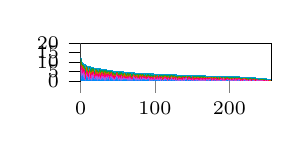
\begin{tikzpicture}

\definecolor{chocolate1961050}{RGB}{196,105,0}
\definecolor{crimson255078}{RGB}{255,0,78}
\definecolor{darkgray153}{RGB}{153,153,153}
\definecolor{darkslategray38}{RGB}{38,38,38}
\definecolor{darkslategray51}{RGB}{51,51,51}
\definecolor{darkturquoise0155207}{RGB}{0,155,207}
\definecolor{deeppink2510138}{RGB}{251,0,138}
\definecolor{dodgerblue0138250}{RGB}{0,138,250}
\definecolor{lightgray204}{RGB}{204,204,204}
\definecolor{mediumorchid21958191}{RGB}{219,58,191}
\definecolor{mediumpurple16495229}{RGB}{164,95,229}
\definecolor{olivedrab851440}{RGB}{85,144,0}
\definecolor{royalblue60122251}{RGB}{60,122,251}
\definecolor{teal015699}{RGB}{0,156,99}

\begin{axis}[
width=0.33\textwidth,
height=0.17\textwidth,
tick label style={font=\scriptsize},
tick align=outside,
tick pos=left,
xmin=0, xmax=256,
y grid style={darkgray176},
ymin=0, ymax=20,
ytick style={color=black},
ytick={0,5,10,15,20},
]
\addplot [semithick, darkgray153, forget plot]
table {%
0 4.44089209850063e-16
0 20
};
\draw[draw=none,fill=dodgerblue0138250] (axis cs:-0.35,0) rectangle (axis cs:0.35,3.21209079667391);

\draw[draw=none,fill=dodgerblue0138250] (axis cs:0.65,0) rectangle (axis cs:1.35,1.01634601541573);
\draw[draw=none,fill=dodgerblue0138250] (axis cs:1.65,0) rectangle (axis cs:2.35,2.57728241171842);
\draw[draw=none,fill=dodgerblue0138250] (axis cs:2.65,0) rectangle (axis cs:3.35,2.19177564592928);
\draw[draw=none,fill=dodgerblue0138250] (axis cs:3.65,0) rectangle (axis cs:4.35,1.13665592664802);
\draw[draw=none,fill=dodgerblue0138250] (axis cs:4.65,0) rectangle (axis cs:5.35,0.743059691936);
\draw[draw=none,fill=dodgerblue0138250] (axis cs:5.65,0) rectangle (axis cs:6.35,0.844238556576386);
\draw[draw=none,fill=dodgerblue0138250] (axis cs:6.65,0) rectangle (axis cs:7.35,0.30726101933072);
\draw[draw=none,fill=dodgerblue0138250] (axis cs:7.65,0) rectangle (axis cs:8.35,1.31068860779935);
\draw[draw=none,fill=dodgerblue0138250] (axis cs:8.65,0) rectangle (axis cs:9.35,1.4413717938885);
\draw[draw=none,fill=dodgerblue0138250] (axis cs:9.65,0) rectangle (axis cs:10.35,0.600402208584663);
\draw[draw=none,fill=dodgerblue0138250] (axis cs:10.65,0) rectangle (axis cs:11.35,0.822928697131679);
\draw[draw=none,fill=dodgerblue0138250] (axis cs:11.65,0) rectangle (axis cs:12.35,0.507689730519144);
\draw[draw=none,fill=dodgerblue0138250] (axis cs:12.65,0) rectangle (axis cs:13.35,0.442137235592553);
\draw[draw=none,fill=dodgerblue0138250] (axis cs:13.65,0) rectangle (axis cs:14.35,1.95749396918005);
\draw[draw=none,fill=dodgerblue0138250] (axis cs:14.65,0) rectangle (axis cs:15.35,0.229441796571356);
\draw[draw=none,fill=dodgerblue0138250] (axis cs:15.65,0) rectangle (axis cs:16.35,0.333413763402898);
\draw[draw=none,fill=dodgerblue0138250] (axis cs:16.65,0) rectangle (axis cs:17.35,1.04653937397113);
\draw[draw=none,fill=dodgerblue0138250] (axis cs:17.65,0) rectangle (axis cs:18.35,0.405551711829128);
\draw[draw=none,fill=dodgerblue0138250] (axis cs:18.65,0) rectangle (axis cs:19.35,0.68400061515262);
\draw[draw=none,fill=dodgerblue0138250] (axis cs:19.65,0) rectangle (axis cs:20.35,0.289011101522939);
\draw[draw=none,fill=dodgerblue0138250] (axis cs:20.65,0) rectangle (axis cs:21.35,0.283077856066011);
\draw[draw=none,fill=dodgerblue0138250] (axis cs:21.65,0) rectangle (axis cs:22.35,0.39280534648891);
\draw[draw=none,fill=dodgerblue0138250] (axis cs:22.65,0) rectangle (axis cs:23.35,0.679479160896671);
\draw[draw=none,fill=dodgerblue0138250] (axis cs:23.65,0) rectangle (axis cs:24.35,0.403486639570142);
\draw[draw=none,fill=dodgerblue0138250] (axis cs:24.65,0) rectangle (axis cs:25.35,0.550926653505845);
\draw[draw=none,fill=dodgerblue0138250] (axis cs:25.65,0) rectangle (axis cs:26.35,0.377370600838955);
\draw[draw=none,fill=dodgerblue0138250] (axis cs:26.65,0) rectangle (axis cs:27.35,0.668364172913855);
\draw[draw=none,fill=dodgerblue0138250] (axis cs:27.65,0) rectangle (axis cs:28.35,0.582345107133666);
\draw[draw=none,fill=dodgerblue0138250] (axis cs:28.65,0) rectangle (axis cs:29.35,0.282962379298725);
\draw[draw=none,fill=dodgerblue0138250] (axis cs:29.65,0) rectangle (axis cs:30.35,0.482797479006365);
\draw[draw=none,fill=dodgerblue0138250] (axis cs:30.65,0) rectangle (axis cs:31.35,0.680316324818482);
\draw[draw=none,fill=dodgerblue0138250] (axis cs:31.65,0) rectangle (axis cs:32.35,0.282720745784384);
\draw[draw=none,fill=dodgerblue0138250] (axis cs:32.65,0) rectangle (axis cs:33.35,0.449697409616317);
\draw[draw=none,fill=dodgerblue0138250] (axis cs:33.65,0) rectangle (axis cs:34.35,0.380256160326507);
\draw[draw=none,fill=dodgerblue0138250] (axis cs:34.65,0) rectangle (axis cs:35.35,1.30968007507141);
\draw[draw=none,fill=dodgerblue0138250] (axis cs:35.65,0) rectangle (axis cs:36.35,0.612304789530423);
\draw[draw=none,fill=dodgerblue0138250] (axis cs:36.65,0) rectangle (axis cs:37.35,1.05905744343572);
\draw[draw=none,fill=dodgerblue0138250] (axis cs:37.65,0) rectangle (axis cs:38.35,0.36878805074256);
\draw[draw=none,fill=dodgerblue0138250] (axis cs:38.65,0) rectangle (axis cs:39.35,0.341631251797282);
\draw[draw=none,fill=dodgerblue0138250] (axis cs:39.65,0) rectangle (axis cs:40.35,1.01908137924101);
\draw[draw=none,fill=dodgerblue0138250] (axis cs:40.65,0) rectangle (axis cs:41.35,0.572773263798448);
\draw[draw=none,fill=dodgerblue0138250] (axis cs:41.65,0) rectangle (axis cs:42.35,0.392561015108842);
\draw[draw=none,fill=dodgerblue0138250] (axis cs:42.65,0) rectangle (axis cs:43.35,0.581066309072499);
\draw[draw=none,fill=dodgerblue0138250] (axis cs:43.65,0) rectangle (axis cs:44.35,0.295598781840444);
\draw[draw=none,fill=dodgerblue0138250] (axis cs:44.65,0) rectangle (axis cs:45.35,0.238889647697903);
\draw[draw=none,fill=dodgerblue0138250] (axis cs:45.65,0) rectangle (axis cs:46.35,0.278339983558881);
\draw[draw=none,fill=dodgerblue0138250] (axis cs:46.65,0) rectangle (axis cs:47.35,0.71539115311341);
\draw[draw=none,fill=dodgerblue0138250] (axis cs:47.65,0) rectangle (axis cs:48.35,1.13217125515228);
\draw[draw=none,fill=dodgerblue0138250] (axis cs:48.65,0) rectangle (axis cs:49.35,0.592221623553778);
\draw[draw=none,fill=dodgerblue0138250] (axis cs:49.65,0) rectangle (axis cs:50.35,0.442213010610546);
\draw[draw=none,fill=dodgerblue0138250] (axis cs:50.65,0) rectangle (axis cs:51.35,0.510227002802029);
\draw[draw=none,fill=dodgerblue0138250] (axis cs:51.65,0) rectangle (axis cs:52.35,0.75372646200032);
\draw[draw=none,fill=dodgerblue0138250] (axis cs:52.65,0) rectangle (axis cs:53.35,0.348492343780612);
\draw[draw=none,fill=dodgerblue0138250] (axis cs:53.65,0) rectangle (axis cs:54.35,0.404823351831872);
\draw[draw=none,fill=dodgerblue0138250] (axis cs:54.65,0) rectangle (axis cs:55.35,0.295032991459576);
\draw[draw=none,fill=dodgerblue0138250] (axis cs:55.65,0) rectangle (axis cs:56.35,0.253562443913851);
\draw[draw=none,fill=dodgerblue0138250] (axis cs:56.65,0) rectangle (axis cs:57.35,0.558630748949282);
\draw[draw=none,fill=dodgerblue0138250] (axis cs:57.65,0) rectangle (axis cs:58.35,0.802557624083663);
\draw[draw=none,fill=dodgerblue0138250] (axis cs:58.65,0) rectangle (axis cs:59.35,0.399670867029491);
\draw[draw=none,fill=dodgerblue0138250] (axis cs:59.65,0) rectangle (axis cs:60.35,0.330513593093447);
\draw[draw=none,fill=dodgerblue0138250] (axis cs:60.65,0) rectangle (axis cs:61.35,0.611870036453549);
\draw[draw=none,fill=dodgerblue0138250] (axis cs:61.65,0) rectangle (axis cs:62.35,0.828807503284758);
\draw[draw=none,fill=dodgerblue0138250] (axis cs:62.65,0) rectangle (axis cs:63.35,0.222760678090229);
\draw[draw=none,fill=dodgerblue0138250] (axis cs:63.65,0) rectangle (axis cs:64.35,0.195778185845065);
\draw[draw=none,fill=dodgerblue0138250] (axis cs:64.65,0) rectangle (axis cs:65.35,0.541985132164507);
\draw[draw=none,fill=dodgerblue0138250] (axis cs:65.65,0) rectangle (axis cs:66.35,0.380106235034922);
\draw[draw=none,fill=dodgerblue0138250] (axis cs:66.65,0) rectangle (axis cs:67.35,0.321691800127817);
\draw[draw=none,fill=dodgerblue0138250] (axis cs:67.65,0) rectangle (axis cs:68.35,0.443353675660629);
\draw[draw=none,fill=dodgerblue0138250] (axis cs:68.65,0) rectangle (axis cs:69.35,0.120298658919739);
\draw[draw=none,fill=dodgerblue0138250] (axis cs:69.65,0) rectangle (axis cs:70.35,0.56330581982687);
\draw[draw=none,fill=dodgerblue0138250] (axis cs:70.65,0) rectangle (axis cs:71.35,1.0674158534594);
\draw[draw=none,fill=dodgerblue0138250] (axis cs:71.65,0) rectangle (axis cs:72.35,0.573332754624895);
\draw[draw=none,fill=dodgerblue0138250] (axis cs:72.65,0) rectangle (axis cs:73.35,0.878120135936457);
\draw[draw=none,fill=dodgerblue0138250] (axis cs:73.65,0) rectangle (axis cs:74.35,0.28873858849242);
\draw[draw=none,fill=dodgerblue0138250] (axis cs:74.65,0) rectangle (axis cs:75.35,0.404437785855564);
\draw[draw=none,fill=dodgerblue0138250] (axis cs:75.65,0) rectangle (axis cs:76.35,0.352369899382684);
\draw[draw=none,fill=dodgerblue0138250] (axis cs:76.65,0) rectangle (axis cs:77.35,0.247859244111649);
\draw[draw=none,fill=dodgerblue0138250] (axis cs:77.65,0) rectangle (axis cs:78.35,0.295971996084285);
\draw[draw=none,fill=dodgerblue0138250] (axis cs:78.65,0) rectangle (axis cs:79.35,0.28123549466547);
\draw[draw=none,fill=dodgerblue0138250] (axis cs:79.65,0) rectangle (axis cs:80.35,0.324964228652691);
\draw[draw=none,fill=dodgerblue0138250] (axis cs:80.65,0) rectangle (axis cs:81.35,0.150713269824138);
\draw[draw=none,fill=dodgerblue0138250] (axis cs:81.65,0) rectangle (axis cs:82.35,0.822287582078362);
\draw[draw=none,fill=dodgerblue0138250] (axis cs:82.65,0) rectangle (axis cs:83.35,0.398154595381184);
\draw[draw=none,fill=dodgerblue0138250] (axis cs:83.65,0) rectangle (axis cs:84.35,0.438224347435992);
\draw[draw=none,fill=dodgerblue0138250] (axis cs:84.65,0) rectangle (axis cs:85.35,0.430751927115982);
\draw[draw=none,fill=dodgerblue0138250] (axis cs:85.65,0) rectangle (axis cs:86.35,0.794870126307537);
\draw[draw=none,fill=dodgerblue0138250] (axis cs:86.65,0) rectangle (axis cs:87.35,0.617833780264471);
\draw[draw=none,fill=dodgerblue0138250] (axis cs:87.65,0) rectangle (axis cs:88.35,0.465090354490452);
\draw[draw=none,fill=dodgerblue0138250] (axis cs:88.65,0) rectangle (axis cs:89.35,0.451834972163776);
\draw[draw=none,fill=dodgerblue0138250] (axis cs:89.65,0) rectangle (axis cs:90.35,0.513741000497242);
\draw[draw=none,fill=dodgerblue0138250] (axis cs:90.65,0) rectangle (axis cs:91.35,0.340666887530637);
\draw[draw=none,fill=dodgerblue0138250] (axis cs:91.65,0) rectangle (axis cs:92.35,0.270505333120898);
\draw[draw=none,fill=dodgerblue0138250] (axis cs:92.65,0) rectangle (axis cs:93.35,0.479556868812455);
\draw[draw=none,fill=dodgerblue0138250] (axis cs:93.65,0) rectangle (axis cs:94.35,0.672898409355151);
\draw[draw=none,fill=dodgerblue0138250] (axis cs:94.65,0) rectangle (axis cs:95.35,0.26570392479091);
\draw[draw=none,fill=dodgerblue0138250] (axis cs:95.65,0) rectangle (axis cs:96.35,0.276998361829052);
\draw[draw=none,fill=dodgerblue0138250] (axis cs:96.65,0) rectangle (axis cs:97.35,0.264028646417605);
\draw[draw=none,fill=dodgerblue0138250] (axis cs:97.65,0) rectangle (axis cs:98.35,0.236509778561023);
\draw[draw=none,fill=dodgerblue0138250] (axis cs:98.65,0) rectangle (axis cs:99.35,0.152565958582894);
\draw[draw=none,fill=dodgerblue0138250] (axis cs:99.65,0) rectangle (axis cs:100.35,0.687093897526739);
\draw[draw=none,fill=dodgerblue0138250] (axis cs:100.65,0) rectangle (axis cs:101.35,0.278584152146277);
\draw[draw=none,fill=dodgerblue0138250] (axis cs:101.65,0) rectangle (axis cs:102.35,0.292683693745141);
\draw[draw=none,fill=dodgerblue0138250] (axis cs:102.65,0) rectangle (axis cs:103.35,0.215509250959551);
\draw[draw=none,fill=dodgerblue0138250] (axis cs:103.65,0) rectangle (axis cs:104.35,0.547519961811641);
\draw[draw=none,fill=dodgerblue0138250] (axis cs:104.65,0) rectangle (axis cs:105.35,0.301562432808571);
\draw[draw=none,fill=dodgerblue0138250] (axis cs:105.65,0) rectangle (axis cs:106.35,0.644578764814461);
\draw[draw=none,fill=dodgerblue0138250] (axis cs:106.65,0) rectangle (axis cs:107.35,0.135935727569186);
\draw[draw=none,fill=dodgerblue0138250] (axis cs:107.65,0) rectangle (axis cs:108.35,0.360415734439763);
\draw[draw=none,fill=dodgerblue0138250] (axis cs:108.65,0) rectangle (axis cs:109.35,0.329139398149682);
\draw[draw=none,fill=dodgerblue0138250] (axis cs:109.65,0) rectangle (axis cs:110.35,0.218163602578833);
\draw[draw=none,fill=dodgerblue0138250] (axis cs:110.65,0) rectangle (axis cs:111.35,0.32232966869273);
\draw[draw=none,fill=dodgerblue0138250] (axis cs:111.65,0) rectangle (axis cs:112.35,0.533790045513198);
\draw[draw=none,fill=dodgerblue0138250] (axis cs:112.65,0) rectangle (axis cs:113.35,0.786450764877463);
\draw[draw=none,fill=dodgerblue0138250] (axis cs:113.65,0) rectangle (axis cs:114.35,0.483249295981095);
\draw[draw=none,fill=dodgerblue0138250] (axis cs:114.65,0) rectangle (axis cs:115.35,0.347494104213622);
\draw[draw=none,fill=dodgerblue0138250] (axis cs:115.65,0) rectangle (axis cs:116.35,0.233514921707825);
\draw[draw=none,fill=dodgerblue0138250] (axis cs:116.65,0) rectangle (axis cs:117.35,0.108402009017732);
\draw[draw=none,fill=dodgerblue0138250] (axis cs:117.65,0) rectangle (axis cs:118.35,0.36782041997096);
\draw[draw=none,fill=dodgerblue0138250] (axis cs:118.65,0) rectangle (axis cs:119.35,0.145726041474465);
\draw[draw=none,fill=dodgerblue0138250] (axis cs:119.65,0) rectangle (axis cs:120.35,0.245707901882769);
\draw[draw=none,fill=dodgerblue0138250] (axis cs:120.65,0) rectangle (axis cs:121.35,0.265389821612132);
\draw[draw=none,fill=dodgerblue0138250] (axis cs:121.65,0) rectangle (axis cs:122.35,0.394078777545445);
\draw[draw=none,fill=dodgerblue0138250] (axis cs:122.65,0) rectangle (axis cs:123.35,0.368259392172507);
\draw[draw=none,fill=dodgerblue0138250] (axis cs:123.65,0) rectangle (axis cs:124.35,0.578758423454975);
\draw[draw=none,fill=dodgerblue0138250] (axis cs:124.65,0) rectangle (axis cs:125.35,0.409272183712562);
\draw[draw=none,fill=dodgerblue0138250] (axis cs:125.65,0) rectangle (axis cs:126.35,0.371118497355122);
\draw[draw=none,fill=dodgerblue0138250] (axis cs:126.65,0) rectangle (axis cs:127.35,0.132050528892913);
\draw[draw=none,fill=dodgerblue0138250] (axis cs:127.65,0) rectangle (axis cs:128.35,0.744242181953237);
\draw[draw=none,fill=dodgerblue0138250] (axis cs:128.65,0) rectangle (axis cs:129.35,0.167125628578751);
\draw[draw=none,fill=dodgerblue0138250] (axis cs:129.65,0) rectangle (axis cs:130.35,0.206523606354712);
\draw[draw=none,fill=dodgerblue0138250] (axis cs:130.65,0) rectangle (axis cs:131.35,0.260723882946624);
\draw[draw=none,fill=dodgerblue0138250] (axis cs:131.65,0) rectangle (axis cs:132.35,0.239740372925874);
\draw[draw=none,fill=dodgerblue0138250] (axis cs:132.65,0) rectangle (axis cs:133.35,0.303740951900606);
\draw[draw=none,fill=dodgerblue0138250] (axis cs:133.65,0) rectangle (axis cs:134.35,0.328369074171747);
\draw[draw=none,fill=dodgerblue0138250] (axis cs:134.65,0) rectangle (axis cs:135.35,0.223253233569149);
\draw[draw=none,fill=dodgerblue0138250] (axis cs:135.65,0) rectangle (axis cs:136.35,0.258534702386344);
\draw[draw=none,fill=dodgerblue0138250] (axis cs:136.65,0) rectangle (axis cs:137.35,0.309409178055524);
\draw[draw=none,fill=dodgerblue0138250] (axis cs:137.65,0) rectangle (axis cs:138.35,0.488644611381616);
\draw[draw=none,fill=dodgerblue0138250] (axis cs:138.65,0) rectangle (axis cs:139.35,0.0762052597906405);
\draw[draw=none,fill=dodgerblue0138250] (axis cs:139.65,0) rectangle (axis cs:140.35,0.366134037920001);
\draw[draw=none,fill=dodgerblue0138250] (axis cs:140.65,0) rectangle (axis cs:141.35,0.499575095879736);
\draw[draw=none,fill=dodgerblue0138250] (axis cs:141.65,0) rectangle (axis cs:142.35,0.433126330472753);
\draw[draw=none,fill=dodgerblue0138250] (axis cs:142.65,0) rectangle (axis cs:143.35,0.267627490623874);
\draw[draw=none,fill=dodgerblue0138250] (axis cs:143.65,0) rectangle (axis cs:144.35,0.17608728620578);
\draw[draw=none,fill=dodgerblue0138250] (axis cs:144.65,0) rectangle (axis cs:145.35,0.44938550578478);
\draw[draw=none,fill=dodgerblue0138250] (axis cs:145.65,0) rectangle (axis cs:146.35,0.118764436881304);
\draw[draw=none,fill=dodgerblue0138250] (axis cs:146.65,0) rectangle (axis cs:147.35,0.3387581276033);
\draw[draw=none,fill=dodgerblue0138250] (axis cs:147.65,0) rectangle (axis cs:148.35,0.407818781610902);
\draw[draw=none,fill=dodgerblue0138250] (axis cs:148.65,0) rectangle (axis cs:149.35,0.0832357363528029);
\draw[draw=none,fill=dodgerblue0138250] (axis cs:149.65,0) rectangle (axis cs:150.35,0.151374766646866);
\draw[draw=none,fill=dodgerblue0138250] (axis cs:150.65,0) rectangle (axis cs:151.35,0.18870792965215);
\draw[draw=none,fill=dodgerblue0138250] (axis cs:151.65,0) rectangle (axis cs:152.35,0.129731831693069);
\draw[draw=none,fill=dodgerblue0138250] (axis cs:152.65,0) rectangle (axis cs:153.35,0.320471686815024);
\draw[draw=none,fill=dodgerblue0138250] (axis cs:153.65,0) rectangle (axis cs:154.35,0.274473209691277);
\draw[draw=none,fill=dodgerblue0138250] (axis cs:154.65,0) rectangle (axis cs:155.35,0.483822380652842);
\draw[draw=none,fill=dodgerblue0138250] (axis cs:155.65,0) rectangle (axis cs:156.35,0.359354153197771);
\draw[draw=none,fill=dodgerblue0138250] (axis cs:156.65,0) rectangle (axis cs:157.35,0.274716905238474);
\draw[draw=none,fill=dodgerblue0138250] (axis cs:157.65,0) rectangle (axis cs:158.35,0.221326782060216);
\draw[draw=none,fill=dodgerblue0138250] (axis cs:158.65,0) rectangle (axis cs:159.35,0.112150687540066);
\draw[draw=none,fill=dodgerblue0138250] (axis cs:159.65,0) rectangle (axis cs:160.35,0.319195546241041);
\draw[draw=none,fill=dodgerblue0138250] (axis cs:160.65,0) rectangle (axis cs:161.35,0.166997697108436);
\draw[draw=none,fill=dodgerblue0138250] (axis cs:161.65,0) rectangle (axis cs:162.35,0.286827981898461);
\draw[draw=none,fill=dodgerblue0138250] (axis cs:162.65,0) rectangle (axis cs:163.35,0.417571332832228);
\draw[draw=none,fill=dodgerblue0138250] (axis cs:163.65,0) rectangle (axis cs:164.35,0.172306337247776);
\draw[draw=none,fill=dodgerblue0138250] (axis cs:164.65,0) rectangle (axis cs:165.35,0.348000475486958);
\draw[draw=none,fill=dodgerblue0138250] (axis cs:165.65,0) rectangle (axis cs:166.35,0.389914148377504);
\draw[draw=none,fill=dodgerblue0138250] (axis cs:166.65,0) rectangle (axis cs:167.35,0.235355380485699);
\draw[draw=none,fill=dodgerblue0138250] (axis cs:167.65,0) rectangle (axis cs:168.35,0.209001837517418);
\draw[draw=none,fill=dodgerblue0138250] (axis cs:168.65,0) rectangle (axis cs:169.35,0.336400467205905);
\draw[draw=none,fill=dodgerblue0138250] (axis cs:169.65,0) rectangle (axis cs:170.35,0.407360332708515);
\draw[draw=none,fill=dodgerblue0138250] (axis cs:170.65,0) rectangle (axis cs:171.35,0.277247662706981);
\draw[draw=none,fill=dodgerblue0138250] (axis cs:171.65,0) rectangle (axis cs:172.35,0.278380826554321);
\draw[draw=none,fill=dodgerblue0138250] (axis cs:172.65,0) rectangle (axis cs:173.35,0.365625427067997);
\draw[draw=none,fill=dodgerblue0138250] (axis cs:173.65,0) rectangle (axis cs:174.35,0.318929575117697);
\draw[draw=none,fill=dodgerblue0138250] (axis cs:174.65,0) rectangle (axis cs:175.35,0.208846167285517);
\draw[draw=none,fill=dodgerblue0138250] (axis cs:175.65,0) rectangle (axis cs:176.35,0.0755052036923116);
\draw[draw=none,fill=dodgerblue0138250] (axis cs:176.65,0) rectangle (axis cs:177.35,0.127589647353554);
\draw[draw=none,fill=dodgerblue0138250] (axis cs:177.65,0) rectangle (axis cs:178.35,0.121759947452429);
\draw[draw=none,fill=dodgerblue0138250] (axis cs:178.65,0) rectangle (axis cs:179.35,0.160351559126796);
\draw[draw=none,fill=dodgerblue0138250] (axis cs:179.65,0) rectangle (axis cs:180.35,0.134672740217149);
\draw[draw=none,fill=dodgerblue0138250] (axis cs:180.65,0) rectangle (axis cs:181.35,0.114836145643582);
\draw[draw=none,fill=dodgerblue0138250] (axis cs:181.65,0) rectangle (axis cs:182.35,0.140914937629898);
\draw[draw=none,fill=dodgerblue0138250] (axis cs:182.65,0) rectangle (axis cs:183.35,0.306096250051192);
\draw[draw=none,fill=dodgerblue0138250] (axis cs:183.65,0) rectangle (axis cs:184.35,0.0723834195110739);
\draw[draw=none,fill=dodgerblue0138250] (axis cs:184.65,0) rectangle (axis cs:185.35,0.100018921574044);
\draw[draw=none,fill=dodgerblue0138250] (axis cs:185.65,0) rectangle (axis cs:186.35,0.133939265301435);
\draw[draw=none,fill=dodgerblue0138250] (axis cs:186.65,0) rectangle (axis cs:187.35,0.143945633643541);
\draw[draw=none,fill=dodgerblue0138250] (axis cs:187.65,0) rectangle (axis cs:188.35,0.388376328285249);
\draw[draw=none,fill=dodgerblue0138250] (axis cs:188.65,0) rectangle (axis cs:189.35,0.220107319214474);
\draw[draw=none,fill=dodgerblue0138250] (axis cs:189.65,0) rectangle (axis cs:190.35,0.314008315711936);
\draw[draw=none,fill=dodgerblue0138250] (axis cs:190.65,0) rectangle (axis cs:191.35,0.23115997322402);
\draw[draw=none,fill=dodgerblue0138250] (axis cs:191.65,0) rectangle (axis cs:192.35,0.17308003120221);
\draw[draw=none,fill=dodgerblue0138250] (axis cs:192.65,0) rectangle (axis cs:193.35,0.149834252867762);
\draw[draw=none,fill=dodgerblue0138250] (axis cs:193.65,0) rectangle (axis cs:194.35,0.178433675280405);
\draw[draw=none,fill=dodgerblue0138250] (axis cs:194.65,0) rectangle (axis cs:195.35,0.393086102973491);
\draw[draw=none,fill=dodgerblue0138250] (axis cs:195.65,0) rectangle (axis cs:196.35,0.287678330584832);
\draw[draw=none,fill=dodgerblue0138250] (axis cs:196.65,0) rectangle (axis cs:197.35,0.820381080735211);
\draw[draw=none,fill=dodgerblue0138250] (axis cs:197.65,0) rectangle (axis cs:198.35,0.321660577675472);
\draw[draw=none,fill=dodgerblue0138250] (axis cs:198.65,0) rectangle (axis cs:199.35,0.286990128615815);
\draw[draw=none,fill=dodgerblue0138250] (axis cs:199.65,0) rectangle (axis cs:200.35,0.193561630490231);
\draw[draw=none,fill=dodgerblue0138250] (axis cs:200.65,0) rectangle (axis cs:201.35,0.308464583981821);
\draw[draw=none,fill=dodgerblue0138250] (axis cs:201.65,0) rectangle (axis cs:202.35,0.292897906876051);
\draw[draw=none,fill=dodgerblue0138250] (axis cs:202.65,0) rectangle (axis cs:203.35,0.191514336809569);
\draw[draw=none,fill=dodgerblue0138250] (axis cs:203.65,0) rectangle (axis cs:204.35,0.118228071945546);
\draw[draw=none,fill=dodgerblue0138250] (axis cs:204.65,0) rectangle (axis cs:205.35,0.18211816657147);
\draw[draw=none,fill=dodgerblue0138250] (axis cs:205.65,0) rectangle (axis cs:206.35,0.344206194023125);
\draw[draw=none,fill=dodgerblue0138250] (axis cs:206.65,0) rectangle (axis cs:207.35,0.0993941302033083);
\draw[draw=none,fill=dodgerblue0138250] (axis cs:207.65,0) rectangle (axis cs:208.35,0.241455322134431);
\draw[draw=none,fill=dodgerblue0138250] (axis cs:208.65,0) rectangle (axis cs:209.35,0.350676581593326);
\draw[draw=none,fill=dodgerblue0138250] (axis cs:209.65,0) rectangle (axis cs:210.35,0.208786808069473);
\draw[draw=none,fill=dodgerblue0138250] (axis cs:210.65,0) rectangle (axis cs:211.35,0.358536230491235);
\draw[draw=none,fill=dodgerblue0138250] (axis cs:211.65,0) rectangle (axis cs:212.35,0.296079119716872);
\draw[draw=none,fill=dodgerblue0138250] (axis cs:212.65,0) rectangle (axis cs:213.35,0.169447388232901);
\draw[draw=none,fill=dodgerblue0138250] (axis cs:213.65,0) rectangle (axis cs:214.35,0.164420540056503);
\draw[draw=none,fill=dodgerblue0138250] (axis cs:214.65,0) rectangle (axis cs:215.35,0.137207251280145);
\draw[draw=none,fill=dodgerblue0138250] (axis cs:215.65,0) rectangle (axis cs:216.35,0.264477213505426);
\draw[draw=none,fill=dodgerblue0138250] (axis cs:216.65,0) rectangle (axis cs:217.35,0.132175025797067);
\draw[draw=none,fill=dodgerblue0138250] (axis cs:217.65,0) rectangle (axis cs:218.35,0.252647357423538);
\draw[draw=none,fill=dodgerblue0138250] (axis cs:218.65,0) rectangle (axis cs:219.35,0.135547538797665);
\draw[draw=none,fill=dodgerblue0138250] (axis cs:219.65,0) rectangle (axis cs:220.35,0.32229659493758);
\draw[draw=none,fill=dodgerblue0138250] (axis cs:220.65,0) rectangle (axis cs:221.35,0.166171183256731);
\draw[draw=none,fill=dodgerblue0138250] (axis cs:221.65,0) rectangle (axis cs:222.35,0.211962604405049);
\draw[draw=none,fill=dodgerblue0138250] (axis cs:222.65,0) rectangle (axis cs:223.35,0.148689884651278);
\draw[draw=none,fill=dodgerblue0138250] (axis cs:223.65,0) rectangle (axis cs:224.35,0.149928747448085);
\draw[draw=none,fill=dodgerblue0138250] (axis cs:224.65,0) rectangle (axis cs:225.35,0.139184533236352);
\draw[draw=none,fill=dodgerblue0138250] (axis cs:225.65,0) rectangle (axis cs:226.35,0.152433216747446);
\draw[draw=none,fill=dodgerblue0138250] (axis cs:226.65,0) rectangle (axis cs:227.35,0.230470269789554);
\draw[draw=none,fill=dodgerblue0138250] (axis cs:227.65,0) rectangle (axis cs:228.35,0.291627576740174);
\draw[draw=none,fill=dodgerblue0138250] (axis cs:228.65,0) rectangle (axis cs:229.35,0.135614092004473);
\draw[draw=none,fill=dodgerblue0138250] (axis cs:229.65,0) rectangle (axis cs:230.35,0.169751055095646);
\draw[draw=none,fill=dodgerblue0138250] (axis cs:230.65,0) rectangle (axis cs:231.35,0.423784350985133);
\draw[draw=none,fill=dodgerblue0138250] (axis cs:231.65,0) rectangle (axis cs:232.35,0.182053421533752);
\draw[draw=none,fill=dodgerblue0138250] (axis cs:232.65,0) rectangle (axis cs:233.35,0.104342732495967);
\draw[draw=none,fill=dodgerblue0138250] (axis cs:233.65,0) rectangle (axis cs:234.35,0.0657226161222433);
\draw[draw=none,fill=dodgerblue0138250] (axis cs:234.65,0) rectangle (axis cs:235.35,0.122160834480269);
\draw[draw=none,fill=dodgerblue0138250] (axis cs:235.65,0) rectangle (axis cs:236.35,0.199891443907564);
\draw[draw=none,fill=dodgerblue0138250] (axis cs:236.65,0) rectangle (axis cs:237.35,0.102598018271977);
\draw[draw=none,fill=dodgerblue0138250] (axis cs:237.65,0) rectangle (axis cs:238.35,0.210691838963152);
\draw[draw=none,fill=dodgerblue0138250] (axis cs:238.65,0) rectangle (axis cs:239.35,0.163971164940389);
\draw[draw=none,fill=dodgerblue0138250] (axis cs:239.65,0) rectangle (axis cs:240.35,0.0924552581094834);
\draw[draw=none,fill=dodgerblue0138250] (axis cs:240.65,0) rectangle (axis cs:241.35,0.10099108323915);
\draw[draw=none,fill=dodgerblue0138250] (axis cs:241.65,0) rectangle (axis cs:242.35,0.150887142013503);
\draw[draw=none,fill=dodgerblue0138250] (axis cs:242.65,0) rectangle (axis cs:243.35,0.255906619912944);
\draw[draw=none,fill=dodgerblue0138250] (axis cs:243.65,0) rectangle (axis cs:244.35,0.284316277549875);
\draw[draw=none,fill=dodgerblue0138250] (axis cs:244.65,0) rectangle (axis cs:245.35,0.134696123343963);
\draw[draw=none,fill=dodgerblue0138250] (axis cs:245.65,0) rectangle (axis cs:246.35,0.0515792423528884);
\draw[draw=none,fill=dodgerblue0138250] (axis cs:246.65,0) rectangle (axis cs:247.35,0.112723277090899);
\draw[draw=none,fill=dodgerblue0138250] (axis cs:247.65,0) rectangle (axis cs:248.35,0.158014293521395);
\draw[draw=none,fill=dodgerblue0138250] (axis cs:248.65,0) rectangle (axis cs:249.35,0.109767896232501);
\draw[draw=none,fill=dodgerblue0138250] (axis cs:249.65,0) rectangle (axis cs:250.35,0.162901659687976);
\draw[draw=none,fill=dodgerblue0138250] (axis cs:250.65,0) rectangle (axis cs:251.35,0.0787471922936103);
\draw[draw=none,fill=dodgerblue0138250] (axis cs:251.65,0) rectangle (axis cs:252.35,0.0718288800348029);
\draw[draw=none,fill=dodgerblue0138250] (axis cs:252.65,0) rectangle (axis cs:253.35,0.171212000707174);
\draw[draw=none,fill=dodgerblue0138250] (axis cs:253.65,0) rectangle (axis cs:254.35,0.0610259525084888);
\draw[draw=none,fill=dodgerblue0138250] (axis cs:254.65,0) rectangle (axis cs:255.35,0.172900279671061);
\draw[draw=none,fill=royalblue60122251] (axis cs:-0.35,3.21209079667391) rectangle (axis cs:0.35,3.85921499630361);

\draw[draw=none,fill=royalblue60122251] (axis cs:0.65,1.01634601541573) rectangle (axis cs:1.35,2.56405612053512);
\draw[draw=none,fill=royalblue60122251] (axis cs:1.65,2.57728241171842) rectangle (axis cs:2.35,3.3612926929336);
\draw[draw=none,fill=royalblue60122251] (axis cs:2.65,2.19177564592928) rectangle (axis cs:3.35,3.76392731815324);
\draw[draw=none,fill=royalblue60122251] (axis cs:3.65,1.13665592664802) rectangle (axis cs:4.35,2.01595197283222);
\draw[draw=none,fill=royalblue60122251] (axis cs:4.65,0.743059691936) rectangle (axis cs:5.35,1.76847631391858);
\draw[draw=none,fill=royalblue60122251] (axis cs:5.65,0.844238556576386) rectangle (axis cs:6.35,2.16953463115275);
\draw[draw=none,fill=royalblue60122251] (axis cs:6.65,0.30726101933072) rectangle (axis cs:7.35,0.56665732480629);
\draw[draw=none,fill=royalblue60122251] (axis cs:7.65,1.31068860779935) rectangle (axis cs:8.35,2.91324503334611);
\draw[draw=none,fill=royalblue60122251] (axis cs:8.65,1.4413717938885) rectangle (axis cs:9.35,2.07624696063234);
\draw[draw=none,fill=royalblue60122251] (axis cs:9.65,0.600402208584663) rectangle (axis cs:10.35,1.06408128227209);
\draw[draw=none,fill=royalblue60122251] (axis cs:10.65,0.822928697131679) rectangle (axis cs:11.35,1.00817873819461);
\draw[draw=none,fill=royalblue60122251] (axis cs:11.65,0.507689730519144) rectangle (axis cs:12.35,2.03605024467026);
\draw[draw=none,fill=royalblue60122251] (axis cs:12.65,0.442137235592553) rectangle (axis cs:13.35,1.03440947074354);
\draw[draw=none,fill=royalblue60122251] (axis cs:13.65,1.95749396918005) rectangle (axis cs:14.35,2.77686413839023);
\draw[draw=none,fill=royalblue60122251] (axis cs:14.65,0.229441796571356) rectangle (axis cs:15.35,0.610791607619848);
\draw[draw=none,fill=royalblue60122251] (axis cs:15.65,0.333413763402898) rectangle (axis cs:16.35,1.46300979040227);
\draw[draw=none,fill=royalblue60122251] (axis cs:16.65,1.04653937397113) rectangle (axis cs:17.35,1.87852228159327);
\draw[draw=none,fill=royalblue60122251] (axis cs:17.65,0.405551711829128) rectangle (axis cs:18.35,0.881252249161567);
\draw[draw=none,fill=royalblue60122251] (axis cs:18.65,0.68400061515262) rectangle (axis cs:19.35,1.35816994542481);
\draw[draw=none,fill=royalblue60122251] (axis cs:19.65,0.289011101522939) rectangle (axis cs:20.35,1.51114908436668);
\draw[draw=none,fill=royalblue60122251] (axis cs:20.65,0.283077856066011) rectangle (axis cs:21.35,0.923340019996504);
\draw[draw=none,fill=royalblue60122251] (axis cs:21.65,0.39280534648891) rectangle (axis cs:22.35,0.629988423865882);
\draw[draw=none,fill=royalblue60122251] (axis cs:22.65,0.679479160896671) rectangle (axis cs:23.35,2.00844427396615);
\draw[draw=none,fill=royalblue60122251] (axis cs:23.65,0.403486639570142) rectangle (axis cs:24.35,1.10430316158218);
\draw[draw=none,fill=royalblue60122251] (axis cs:24.65,0.550926653505845) rectangle (axis cs:25.35,1.05407672363195);
\draw[draw=none,fill=royalblue60122251] (axis cs:25.65,0.377370600838955) rectangle (axis cs:26.35,0.822580673461859);
\draw[draw=none,fill=royalblue60122251] (axis cs:26.65,0.668364172913855) rectangle (axis cs:27.35,1.65853250598665);
\draw[draw=none,fill=royalblue60122251] (axis cs:27.65,0.582345107133666) rectangle (axis cs:28.35,0.811875369910918);
\draw[draw=none,fill=royalblue60122251] (axis cs:28.65,0.282962379298725) rectangle (axis cs:29.35,1.28829370210058);
\draw[draw=none,fill=royalblue60122251] (axis cs:29.65,0.482797479006365) rectangle (axis cs:30.35,0.780441346888568);
\draw[draw=none,fill=royalblue60122251] (axis cs:30.65,0.680316324818482) rectangle (axis cs:31.35,1.51965479009072);
\draw[draw=none,fill=royalblue60122251] (axis cs:31.65,0.282720745784384) rectangle (axis cs:32.35,0.466814958983016);
\draw[draw=none,fill=royalblue60122251] (axis cs:32.65,0.449697409616317) rectangle (axis cs:33.35,0.583776458550496);
\draw[draw=none,fill=royalblue60122251] (axis cs:33.65,0.380256160326507) rectangle (axis cs:34.35,1.37323440939325);
\draw[draw=none,fill=royalblue60122251] (axis cs:34.65,1.30968007507141) rectangle (axis cs:35.35,1.99820605316506);
\draw[draw=none,fill=royalblue60122251] (axis cs:35.65,0.612304789530423) rectangle (axis cs:36.35,0.990295900605613);
\draw[draw=none,fill=royalblue60122251] (axis cs:36.65,1.05905744343572) rectangle (axis cs:37.35,2.13827181997592);
\draw[draw=none,fill=royalblue60122251] (axis cs:37.65,0.36878805074256) rectangle (axis cs:38.35,0.982486628638969);
\draw[draw=none,fill=royalblue60122251] (axis cs:38.65,0.341631251797282) rectangle (axis cs:39.35,0.617831608078828);
\draw[draw=none,fill=royalblue60122251] (axis cs:39.65,1.01908137924101) rectangle (axis cs:40.35,1.93933109155864);
\draw[draw=none,fill=royalblue60122251] (axis cs:40.65,0.572773263798448) rectangle (axis cs:41.35,1.70714181668055);
\draw[draw=none,fill=royalblue60122251] (axis cs:41.65,0.392561015108842) rectangle (axis cs:42.35,0.810443264596312);
\draw[draw=none,fill=royalblue60122251] (axis cs:42.65,0.581066309072499) rectangle (axis cs:43.35,1.59309093266679);
\draw[draw=none,fill=royalblue60122251] (axis cs:43.65,0.295598781840444) rectangle (axis cs:44.35,0.409901899575042);
\draw[draw=none,fill=royalblue60122251] (axis cs:44.65,0.238889647697903) rectangle (axis cs:45.35,0.663925747463777);
\draw[draw=none,fill=royalblue60122251] (axis cs:45.65,0.278339983558881) rectangle (axis cs:46.35,1.03678320893811);
\draw[draw=none,fill=royalblue60122251] (axis cs:46.65,0.71539115311341) rectangle (axis cs:47.35,1.74842738598359);
\draw[draw=none,fill=royalblue60122251] (axis cs:47.65,1.13217125515228) rectangle (axis cs:48.35,1.86521882121591);
\draw[draw=none,fill=royalblue60122251] (axis cs:48.65,0.592221623553778) rectangle (axis cs:49.35,1.38198737885198);
\draw[draw=none,fill=royalblue60122251] (axis cs:49.65,0.442213010610546) rectangle (axis cs:50.35,0.641539588427305);
\draw[draw=none,fill=royalblue60122251] (axis cs:50.65,0.510227002802029) rectangle (axis cs:51.35,0.936605542351377);
\draw[draw=none,fill=royalblue60122251] (axis cs:51.65,0.75372646200032) rectangle (axis cs:52.35,1.07175017069579);
\draw[draw=none,fill=royalblue60122251] (axis cs:52.65,0.348492343780612) rectangle (axis cs:53.35,0.620361903701386);
\draw[draw=none,fill=royalblue60122251] (axis cs:53.65,0.404823351831872) rectangle (axis cs:54.35,0.812917091638228);
\draw[draw=none,fill=royalblue60122251] (axis cs:54.65,0.295032991459576) rectangle (axis cs:55.35,0.68047742887263);
\draw[draw=none,fill=royalblue60122251] (axis cs:55.65,0.253562443913851) rectangle (axis cs:56.35,0.869113323367846);
\draw[draw=none,fill=royalblue60122251] (axis cs:56.65,0.558630748949282) rectangle (axis cs:57.35,0.862501308400215);
\draw[draw=none,fill=royalblue60122251] (axis cs:57.65,0.802557624083663) rectangle (axis cs:58.35,1.21110758017611);
\draw[draw=none,fill=royalblue60122251] (axis cs:58.65,0.399670867029491) rectangle (axis cs:59.35,1.25516495713172);
\draw[draw=none,fill=royalblue60122251] (axis cs:59.65,0.330513593093447) rectangle (axis cs:60.35,1.12504177080928);
\draw[draw=none,fill=royalblue60122251] (axis cs:60.65,0.611870036453549) rectangle (axis cs:61.35,1.45837281020627);
\draw[draw=none,fill=royalblue60122251] (axis cs:61.65,0.828807503284758) rectangle (axis cs:62.35,1.35641940560964);
\draw[draw=none,fill=royalblue60122251] (axis cs:62.65,0.222760678090229) rectangle (axis cs:63.35,0.675480507037307);
\draw[draw=none,fill=royalblue60122251] (axis cs:63.65,0.195778185845065) rectangle (axis cs:64.35,0.749413475900868);
\draw[draw=none,fill=royalblue60122251] (axis cs:64.65,0.541985132164507) rectangle (axis cs:65.35,1.49012851330038);
\draw[draw=none,fill=royalblue60122251] (axis cs:65.65,0.380106235034922) rectangle (axis cs:66.35,0.534513020714311);
\draw[draw=none,fill=royalblue60122251] (axis cs:66.65,0.321691800127817) rectangle (axis cs:67.35,0.541086127177307);
\draw[draw=none,fill=royalblue60122251] (axis cs:67.65,0.443353675660629) rectangle (axis cs:68.35,0.635242635069705);
\draw[draw=none,fill=royalblue60122251] (axis cs:68.65,0.120298658919739) rectangle (axis cs:69.35,0.464867766459305);
\draw[draw=none,fill=royalblue60122251] (axis cs:69.65,0.56330581982687) rectangle (axis cs:70.35,0.894242551299888);
\draw[draw=none,fill=royalblue60122251] (axis cs:70.65,1.0674158534594) rectangle (axis cs:71.35,1.66764513072409);
\draw[draw=none,fill=royalblue60122251] (axis cs:71.65,0.573332754624895) rectangle (axis cs:72.35,0.888016350601557);
\draw[draw=none,fill=royalblue60122251] (axis cs:72.65,0.878120135936457) rectangle (axis cs:73.35,1.74366860147232);
\draw[draw=none,fill=royalblue60122251] (axis cs:73.65,0.28873858849242) rectangle (axis cs:74.35,0.467803069007319);
\draw[draw=none,fill=royalblue60122251] (axis cs:74.65,0.404437785855564) rectangle (axis cs:75.35,0.725664808627884);
\draw[draw=none,fill=royalblue60122251] (axis cs:75.65,0.352369899382684) rectangle (axis cs:76.35,1.07173212485967);
\draw[draw=none,fill=royalblue60122251] (axis cs:76.65,0.247859244111649) rectangle (axis cs:77.35,0.534671699310209);
\draw[draw=none,fill=royalblue60122251] (axis cs:77.65,0.295971996084285) rectangle (axis cs:78.35,0.622334350393741);
\draw[draw=none,fill=royalblue60122251] (axis cs:78.65,0.28123549466547) rectangle (axis cs:79.35,0.640357451544192);
\draw[draw=none,fill=royalblue60122251] (axis cs:79.65,0.324964228652691) rectangle (axis cs:80.35,1.14778530483071);
\draw[draw=none,fill=royalblue60122251] (axis cs:80.65,0.150713269824138) rectangle (axis cs:81.35,0.792971236250707);
\draw[draw=none,fill=royalblue60122251] (axis cs:81.65,0.822287582078362) rectangle (axis cs:82.35,1.06047266842306);
\draw[draw=none,fill=royalblue60122251] (axis cs:82.65,0.398154595381184) rectangle (axis cs:83.35,1.08900073392419);
\draw[draw=none,fill=royalblue60122251] (axis cs:83.65,0.438224347435992) rectangle (axis cs:84.35,0.880970237871387);
\draw[draw=none,fill=royalblue60122251] (axis cs:84.65,0.430751927115982) rectangle (axis cs:85.35,1.23070310323207);
\draw[draw=none,fill=royalblue60122251] (axis cs:85.65,0.794870126307537) rectangle (axis cs:86.35,1.25283992904159);
\draw[draw=none,fill=royalblue60122251] (axis cs:86.65,0.617833780264471) rectangle (axis cs:87.35,0.887517380404905);
\draw[draw=none,fill=royalblue60122251] (axis cs:87.65,0.465090354490452) rectangle (axis cs:88.35,0.752993063192722);
\draw[draw=none,fill=royalblue60122251] (axis cs:88.65,0.451834972163776) rectangle (axis cs:89.35,1.15835618084966);
\draw[draw=none,fill=royalblue60122251] (axis cs:89.65,0.513741000497242) rectangle (axis cs:90.35,1.01761059657385);
\draw[draw=none,fill=royalblue60122251] (axis cs:90.65,0.340666887530637) rectangle (axis cs:91.35,0.889561908501638);
\draw[draw=none,fill=royalblue60122251] (axis cs:91.65,0.270505333120898) rectangle (axis cs:92.35,0.619959549937111);
\draw[draw=none,fill=royalblue60122251] (axis cs:92.65,0.479556868812455) rectangle (axis cs:93.35,0.715115317566606);
\draw[draw=none,fill=royalblue60122251] (axis cs:93.65,0.672898409355151) rectangle (axis cs:94.35,0.8372232944869);
\draw[draw=none,fill=royalblue60122251] (axis cs:94.65,0.26570392479091) rectangle (axis cs:95.35,0.686141499670284);
\draw[draw=none,fill=royalblue60122251] (axis cs:95.65,0.276998361829052) rectangle (axis cs:96.35,0.718251612059504);
\draw[draw=none,fill=royalblue60122251] (axis cs:96.65,0.264028646417605) rectangle (axis cs:97.35,0.93437246433081);
\draw[draw=none,fill=royalblue60122251] (axis cs:97.65,0.236509778561023) rectangle (axis cs:98.35,0.777201809676916);
\draw[draw=none,fill=royalblue60122251] (axis cs:98.65,0.152565958582894) rectangle (axis cs:99.35,0.820057322638027);
\draw[draw=none,fill=royalblue60122251] (axis cs:99.65,0.687093897526739) rectangle (axis cs:100.35,0.905653082764459);
\draw[draw=none,fill=royalblue60122251] (axis cs:100.65,0.278584152146277) rectangle (axis cs:101.35,0.903335648273597);
\draw[draw=none,fill=royalblue60122251] (axis cs:101.65,0.292683693745141) rectangle (axis cs:102.35,0.777962507075313);
\draw[draw=none,fill=royalblue60122251] (axis cs:102.65,0.215509250959551) rectangle (axis cs:103.35,0.334481451898703);
\draw[draw=none,fill=royalblue60122251] (axis cs:103.65,0.547519961811641) rectangle (axis cs:104.35,0.659335231711528);
\draw[draw=none,fill=royalblue60122251] (axis cs:104.65,0.301562432808571) rectangle (axis cs:105.35,0.599074192226767);
\draw[draw=none,fill=royalblue60122251] (axis cs:105.65,0.644578764814461) rectangle (axis cs:106.35,0.849861866848268);
\draw[draw=none,fill=royalblue60122251] (axis cs:106.65,0.135935727569186) rectangle (axis cs:107.35,0.266651090627233);
\draw[draw=none,fill=royalblue60122251] (axis cs:107.65,0.360415734439763) rectangle (axis cs:108.35,0.979334681616195);
\draw[draw=none,fill=royalblue60122251] (axis cs:108.65,0.329139398149682) rectangle (axis cs:109.35,1.02992355690905);
\draw[draw=none,fill=royalblue60122251] (axis cs:109.65,0.218163602578833) rectangle (axis cs:110.35,0.356304014193656);
\draw[draw=none,fill=royalblue60122251] (axis cs:110.65,0.32232966869273) rectangle (axis cs:111.35,0.972761049566167);
\draw[draw=none,fill=royalblue60122251] (axis cs:111.65,0.533790045513198) rectangle (axis cs:112.35,0.730757291704316);
\draw[draw=none,fill=royalblue60122251] (axis cs:112.65,0.786450764877463) rectangle (axis cs:113.35,1.13090292419191);
\draw[draw=none,fill=royalblue60122251] (axis cs:113.65,0.483249295981095) rectangle (axis cs:114.35,0.85367224914233);
\draw[draw=none,fill=royalblue60122251] (axis cs:114.65,0.347494104213622) rectangle (axis cs:115.35,0.787046870867358);
\draw[draw=none,fill=royalblue60122251] (axis cs:115.65,0.233514921707825) rectangle (axis cs:116.35,0.810297988272706);
\draw[draw=none,fill=royalblue60122251] (axis cs:116.65,0.108402009017732) rectangle (axis cs:117.35,0.185104319634983);
\draw[draw=none,fill=royalblue60122251] (axis cs:117.65,0.36782041997096) rectangle (axis cs:118.35,1.18350724390148);
\draw[draw=none,fill=royalblue60122251] (axis cs:118.65,0.145726041474465) rectangle (axis cs:119.35,0.45403323621106);
\draw[draw=none,fill=royalblue60122251] (axis cs:119.65,0.245707901882769) rectangle (axis cs:120.35,0.357721077781081);
\draw[draw=none,fill=royalblue60122251] (axis cs:120.65,0.265389821612132) rectangle (axis cs:121.35,0.362662423964468);
\draw[draw=none,fill=royalblue60122251] (axis cs:121.65,0.394078777545445) rectangle (axis cs:122.35,0.903030668279638);
\draw[draw=none,fill=royalblue60122251] (axis cs:122.65,0.368259392172507) rectangle (axis cs:123.35,0.70611840052645);
\draw[draw=none,fill=royalblue60122251] (axis cs:123.65,0.578758423454975) rectangle (axis cs:124.35,0.671464775306848);
\draw[draw=none,fill=royalblue60122251] (axis cs:124.65,0.409272183712562) rectangle (axis cs:125.35,1.07419620010764);
\draw[draw=none,fill=royalblue60122251] (axis cs:125.65,0.371118497355122) rectangle (axis cs:126.35,0.76506881178574);
\draw[draw=none,fill=royalblue60122251] (axis cs:126.65,0.132050528892913) rectangle (axis cs:127.35,0.486718062545136);
\draw[draw=none,fill=royalblue60122251] (axis cs:127.65,0.744242181953237) rectangle (axis cs:128.35,1.04488220103304);
\draw[draw=none,fill=royalblue60122251] (axis cs:128.65,0.167125628578751) rectangle (axis cs:129.35,0.877458047422895);
\draw[draw=none,fill=royalblue60122251] (axis cs:129.65,0.206523606354712) rectangle (axis cs:130.35,0.411146503107054);
\draw[draw=none,fill=royalblue60122251] (axis cs:130.65,0.260723882946624) rectangle (axis cs:131.35,0.368760114449115);
\draw[draw=none,fill=royalblue60122251] (axis cs:131.65,0.239740372925874) rectangle (axis cs:132.35,0.880972861112831);
\draw[draw=none,fill=royalblue60122251] (axis cs:132.65,0.303740951900606) rectangle (axis cs:133.35,0.529837633988411);
\draw[draw=none,fill=royalblue60122251] (axis cs:133.65,0.328369074171747) rectangle (axis cs:134.35,0.611887749966157);
\draw[draw=none,fill=royalblue60122251] (axis cs:134.65,0.223253233569149) rectangle (axis cs:135.35,0.509440303018251);
\draw[draw=none,fill=royalblue60122251] (axis cs:135.65,0.258534702386344) rectangle (axis cs:136.35,0.315738876601779);
\draw[draw=none,fill=royalblue60122251] (axis cs:136.65,0.309409178055524) rectangle (axis cs:137.35,1.17873191564192);
\draw[draw=none,fill=royalblue60122251] (axis cs:137.65,0.488644611381616) rectangle (axis cs:138.35,0.628755179977567);
\draw[draw=none,fill=royalblue60122251] (axis cs:138.65,0.0762052597906405) rectangle (axis cs:139.35,0.397815391971696);
\draw[draw=none,fill=royalblue60122251] (axis cs:139.65,0.366134037920001) rectangle (axis cs:140.35,0.627552180563836);
\draw[draw=none,fill=royalblue60122251] (axis cs:140.65,0.499575095879736) rectangle (axis cs:141.35,1.0235201876264);
\draw[draw=none,fill=royalblue60122251] (axis cs:141.65,0.433126330472753) rectangle (axis cs:142.35,0.965606393426826);
\draw[draw=none,fill=royalblue60122251] (axis cs:142.65,0.267627490623874) rectangle (axis cs:143.35,0.358297182906363);
\draw[draw=none,fill=royalblue60122251] (axis cs:143.65,0.17608728620578) rectangle (axis cs:144.35,0.703818309367399);
\draw[draw=none,fill=royalblue60122251] (axis cs:144.65,0.44938550578478) rectangle (axis cs:145.35,0.794028107321616);
\draw[draw=none,fill=royalblue60122251] (axis cs:145.65,0.118764436881304) rectangle (axis cs:146.35,0.633321282743077);
\draw[draw=none,fill=royalblue60122251] (axis cs:146.65,0.3387581276033) rectangle (axis cs:147.35,0.83085699992935);
\draw[draw=none,fill=royalblue60122251] (axis cs:147.65,0.407818781610902) rectangle (axis cs:148.35,0.890710829446631);
\draw[draw=none,fill=royalblue60122251] (axis cs:148.65,0.0832357363528029) rectangle (axis cs:149.35,0.159080762034734);
\draw[draw=none,fill=royalblue60122251] (axis cs:149.65,0.151374766646866) rectangle (axis cs:150.35,0.719717837510004);
\draw[draw=none,fill=royalblue60122251] (axis cs:150.65,0.18870792965215) rectangle (axis cs:151.35,0.446976239113941);
\draw[draw=none,fill=royalblue60122251] (axis cs:151.65,0.129731831693069) rectangle (axis cs:152.35,0.341119950962754);
\draw[draw=none,fill=royalblue60122251] (axis cs:152.65,0.320471686815024) rectangle (axis cs:153.35,0.713258858822683);
\draw[draw=none,fill=royalblue60122251] (axis cs:153.65,0.274473209691277) rectangle (axis cs:154.35,0.350235704241514);
\draw[draw=none,fill=royalblue60122251] (axis cs:154.65,0.483822380652842) rectangle (axis cs:155.35,0.625729736294516);
\draw[draw=none,fill=royalblue60122251] (axis cs:155.65,0.359354153197771) rectangle (axis cs:156.35,0.44136205482573);
\draw[draw=none,fill=royalblue60122251] (axis cs:156.65,0.274716905238474) rectangle (axis cs:157.35,0.662580730778727);
\draw[draw=none,fill=royalblue60122251] (axis cs:157.65,0.221326782060216) rectangle (axis cs:158.35,0.338297770249804);
\draw[draw=none,fill=royalblue60122251] (axis cs:158.65,0.112150687540066) rectangle (axis cs:159.35,0.267652628901776);
\draw[draw=none,fill=royalblue60122251] (axis cs:159.65,0.319195546241041) rectangle (axis cs:160.35,0.695310119735674);
\draw[draw=none,fill=royalblue60122251] (axis cs:160.65,0.166997697108436) rectangle (axis cs:161.35,0.241562278113584);
\draw[draw=none,fill=royalblue60122251] (axis cs:161.65,0.286827981898461) rectangle (axis cs:162.35,0.357720655111541);
\draw[draw=none,fill=royalblue60122251] (axis cs:162.65,0.417571332832228) rectangle (axis cs:163.35,0.52086967264548);
\draw[draw=none,fill=royalblue60122251] (axis cs:163.65,0.172306337247776) rectangle (axis cs:164.35,0.411090872807418);
\draw[draw=none,fill=royalblue60122251] (axis cs:164.65,0.348000475486958) rectangle (axis cs:165.35,0.47532009972007);
\draw[draw=none,fill=royalblue60122251] (axis cs:165.65,0.389914148377504) rectangle (axis cs:166.35,0.530326474293225);
\draw[draw=none,fill=royalblue60122251] (axis cs:166.65,0.235355380485699) rectangle (axis cs:167.35,0.799824170148778);
\draw[draw=none,fill=royalblue60122251] (axis cs:167.65,0.209001837517418) rectangle (axis cs:168.35,0.532664016401005);
\draw[draw=none,fill=royalblue60122251] (axis cs:168.65,0.336400467205905) rectangle (axis cs:169.35,0.658071269199184);
\draw[draw=none,fill=royalblue60122251] (axis cs:169.65,0.407360332708515) rectangle (axis cs:170.35,0.551123495878881);
\draw[draw=none,fill=royalblue60122251] (axis cs:170.65,0.277247662706981) rectangle (axis cs:171.35,0.590657045905756);
\draw[draw=none,fill=royalblue60122251] (axis cs:171.65,0.278380826554321) rectangle (axis cs:172.35,0.414566068825856);
\draw[draw=none,fill=royalblue60122251] (axis cs:172.65,0.365625427067997) rectangle (axis cs:173.35,0.675449342612012);
\draw[draw=none,fill=royalblue60122251] (axis cs:173.65,0.318929575117697) rectangle (axis cs:174.35,0.773773737333242);
\draw[draw=none,fill=royalblue60122251] (axis cs:174.65,0.208846167285517) rectangle (axis cs:175.35,0.559625160569938);
\draw[draw=none,fill=royalblue60122251] (axis cs:175.65,0.0755052036923116) rectangle (axis cs:176.35,0.218054071136525);
\draw[draw=none,fill=royalblue60122251] (axis cs:176.65,0.127589647353554) rectangle (axis cs:177.35,0.381194220291549);
\draw[draw=none,fill=royalblue60122251] (axis cs:177.65,0.121759947452429) rectangle (axis cs:178.35,0.3398708935606);
\draw[draw=none,fill=royalblue60122251] (axis cs:178.65,0.160351559126796) rectangle (axis cs:179.35,0.587403479560921);
\draw[draw=none,fill=royalblue60122251] (axis cs:179.65,0.134672740217149) rectangle (axis cs:180.35,0.288240930045775);
\draw[draw=none,fill=royalblue60122251] (axis cs:180.65,0.114836145643582) rectangle (axis cs:181.35,0.897218365033332);
\draw[draw=none,fill=royalblue60122251] (axis cs:181.65,0.140914937629898) rectangle (axis cs:182.35,0.22286119537724);
\draw[draw=none,fill=royalblue60122251] (axis cs:182.65,0.306096250051192) rectangle (axis cs:183.35,0.522466440590716);
\draw[draw=none,fill=royalblue60122251] (axis cs:183.65,0.0723834195110739) rectangle (axis cs:184.35,0.533174440363154);
\draw[draw=none,fill=royalblue60122251] (axis cs:184.65,0.100018921574044) rectangle (axis cs:185.35,0.481996174080916);
\draw[draw=none,fill=royalblue60122251] (axis cs:185.65,0.133939265301435) rectangle (axis cs:186.35,0.630747073757348);
\draw[draw=none,fill=royalblue60122251] (axis cs:186.65,0.143945633643541) rectangle (axis cs:187.35,0.466343027865407);
\draw[draw=none,fill=royalblue60122251] (axis cs:187.65,0.388376328285249) rectangle (axis cs:188.35,0.657033018964128);
\draw[draw=none,fill=royalblue60122251] (axis cs:188.65,0.220107319214474) rectangle (axis cs:189.35,0.661079748665661);
\draw[draw=none,fill=royalblue60122251] (axis cs:189.65,0.314008315711936) rectangle (axis cs:190.35,0.36421381645939);
\draw[draw=none,fill=royalblue60122251] (axis cs:190.65,0.23115997322402) rectangle (axis cs:191.35,0.337798820001195);
\draw[draw=none,fill=royalblue60122251] (axis cs:191.65,0.17308003120221) rectangle (axis cs:192.35,0.311880759653891);
\draw[draw=none,fill=royalblue60122251] (axis cs:192.65,0.149834252867762) rectangle (axis cs:193.35,0.340317496426389);
\draw[draw=none,fill=royalblue60122251] (axis cs:193.65,0.178433675280405) rectangle (axis cs:194.35,0.401735149276379);
\draw[draw=none,fill=royalblue60122251] (axis cs:194.65,0.393086102973491) rectangle (axis cs:195.35,0.551126949141823);
\draw[draw=none,fill=royalblue60122251] (axis cs:195.65,0.287678330584832) rectangle (axis cs:196.35,0.535503961346272);
\draw[draw=none,fill=royalblue60122251] (axis cs:196.65,0.820381080735211) rectangle (axis cs:197.35,1.00069572458098);
\draw[draw=none,fill=royalblue60122251] (axis cs:197.65,0.321660577675472) rectangle (axis cs:198.35,0.613914020537742);
\draw[draw=none,fill=royalblue60122251] (axis cs:198.65,0.286990128615815) rectangle (axis cs:199.35,0.367971441654842);
\draw[draw=none,fill=royalblue60122251] (axis cs:199.65,0.193561630490231) rectangle (axis cs:200.35,0.297203897063649);
\draw[draw=none,fill=royalblue60122251] (axis cs:200.65,0.308464583981821) rectangle (axis cs:201.35,0.427983990659364);
\draw[draw=none,fill=royalblue60122251] (axis cs:201.65,0.292897906876051) rectangle (axis cs:202.35,0.671111251694594);
\draw[draw=none,fill=royalblue60122251] (axis cs:202.65,0.191514336809569) rectangle (axis cs:203.35,0.269847027430689);
\draw[draw=none,fill=royalblue60122251] (axis cs:203.65,0.118228071945546) rectangle (axis cs:204.35,0.409648711242276);
\draw[draw=none,fill=royalblue60122251] (axis cs:204.65,0.18211816657147) rectangle (axis cs:205.35,0.552012364484061);
\draw[draw=none,fill=royalblue60122251] (axis cs:205.65,0.344206194023125) rectangle (axis cs:206.35,0.492595226130063);
\draw[draw=none,fill=royalblue60122251] (axis cs:206.65,0.0993941302033083) rectangle (axis cs:207.35,0.210933069199357);
\draw[draw=none,fill=royalblue60122251] (axis cs:207.65,0.241455322134431) rectangle (axis cs:208.35,0.370390769769161);
\draw[draw=none,fill=royalblue60122251] (axis cs:208.65,0.350676581593326) rectangle (axis cs:209.35,0.396892839991709);
\draw[draw=none,fill=royalblue60122251] (axis cs:209.65,0.208786808069473) rectangle (axis cs:210.35,0.633626414561805);
\draw[draw=none,fill=royalblue60122251] (axis cs:210.65,0.358536230491235) rectangle (axis cs:211.35,0.470676509242901);
\draw[draw=none,fill=royalblue60122251] (axis cs:211.65,0.296079119716872) rectangle (axis cs:212.35,0.400393640682173);
\draw[draw=none,fill=royalblue60122251] (axis cs:212.65,0.169447388232901) rectangle (axis cs:213.35,0.666245584829791);
\draw[draw=none,fill=royalblue60122251] (axis cs:213.65,0.164420540056503) rectangle (axis cs:214.35,0.483308825515047);
\draw[draw=none,fill=royalblue60122251] (axis cs:214.65,0.137207251280145) rectangle (axis cs:215.35,0.236400597542602);
\draw[draw=none,fill=royalblue60122251] (axis cs:215.65,0.264477213505426) rectangle (axis cs:216.35,0.543839363524991);
\draw[draw=none,fill=royalblue60122251] (axis cs:216.65,0.132175025797067) rectangle (axis cs:217.35,0.189757954058921);
\draw[draw=none,fill=royalblue60122251] (axis cs:217.65,0.252647357423538) rectangle (axis cs:218.35,0.376676039533669);
\draw[draw=none,fill=royalblue60122251] (axis cs:218.65,0.135547538797665) rectangle (axis cs:219.35,0.366073271296279);
\draw[draw=none,fill=royalblue60122251] (axis cs:219.65,0.32229659493758) rectangle (axis cs:220.35,0.437252299242209);
\draw[draw=none,fill=royalblue60122251] (axis cs:220.65,0.166171183256731) rectangle (axis cs:221.35,0.430099055758762);
\draw[draw=none,fill=royalblue60122251] (axis cs:221.65,0.211962604405049) rectangle (axis cs:222.35,0.342390498262086);
\draw[draw=none,fill=royalblue60122251] (axis cs:222.65,0.148689884651278) rectangle (axis cs:223.35,0.254133067223934);
\draw[draw=none,fill=royalblue60122251] (axis cs:223.65,0.149928747448085) rectangle (axis cs:224.35,0.374611002936957);
\draw[draw=none,fill=royalblue60122251] (axis cs:224.65,0.139184533236352) rectangle (axis cs:225.35,0.222634587737339);
\draw[draw=none,fill=royalblue60122251] (axis cs:225.65,0.152433216747446) rectangle (axis cs:226.35,0.333274920704263);
\draw[draw=none,fill=royalblue60122251] (axis cs:226.65,0.230470269789554) rectangle (axis cs:227.35,0.319657791417701);
\draw[draw=none,fill=royalblue60122251] (axis cs:227.65,0.291627576740174) rectangle (axis cs:228.35,0.427720230943536);
\draw[draw=none,fill=royalblue60122251] (axis cs:228.65,0.135614092004473) rectangle (axis cs:229.35,0.201016880517207);
\draw[draw=none,fill=royalblue60122251] (axis cs:229.65,0.169751055095646) rectangle (axis cs:230.35,0.363667435288308);
\draw[draw=none,fill=royalblue60122251] (axis cs:230.65,0.423784350985133) rectangle (axis cs:231.35,0.472173746929306);
\draw[draw=none,fill=royalblue60122251] (axis cs:231.65,0.182053421533752) rectangle (axis cs:232.35,0.53607735029776);
\draw[draw=none,fill=royalblue60122251] (axis cs:232.65,0.104342732495967) rectangle (axis cs:233.35,0.22251285451072);
\draw[draw=none,fill=royalblue60122251] (axis cs:233.65,0.0657226161222433) rectangle (axis cs:234.35,0.127305264863207);
\draw[draw=none,fill=royalblue60122251] (axis cs:234.65,0.122160834480269) rectangle (axis cs:235.35,0.167406209112331);
\draw[draw=none,fill=royalblue60122251] (axis cs:235.65,0.199891443907564) rectangle (axis cs:236.35,0.317833993533556);
\draw[draw=none,fill=royalblue60122251] (axis cs:236.65,0.102598018271977) rectangle (axis cs:237.35,0.404070385026688);
\draw[draw=none,fill=royalblue60122251] (axis cs:237.65,0.210691838963152) rectangle (axis cs:238.35,0.265825601921786);
\draw[draw=none,fill=royalblue60122251] (axis cs:238.65,0.163971164940389) rectangle (axis cs:239.35,0.208128945968013);
\draw[draw=none,fill=royalblue60122251] (axis cs:239.65,0.0924552581094834) rectangle (axis cs:240.35,0.139649518528584);
\draw[draw=none,fill=royalblue60122251] (axis cs:240.65,0.10099108323915) rectangle (axis cs:241.35,0.300360847186482);
\draw[draw=none,fill=royalblue60122251] (axis cs:241.65,0.150887142013503) rectangle (axis cs:242.35,0.200238902483703);
\draw[draw=none,fill=royalblue60122251] (axis cs:242.65,0.255906619912944) rectangle (axis cs:243.35,0.393666986779344);
\draw[draw=none,fill=royalblue60122251] (axis cs:243.65,0.284316277549875) rectangle (axis cs:244.35,0.442704034528227);
\draw[draw=none,fill=royalblue60122251] (axis cs:244.65,0.134696123343963) rectangle (axis cs:245.35,0.248441111201046);
\draw[draw=none,fill=royalblue60122251] (axis cs:245.65,0.0515792423528884) rectangle (axis cs:246.35,0.124462662661193);
\draw[draw=none,fill=royalblue60122251] (axis cs:246.65,0.112723277090899) rectangle (axis cs:247.35,0.155409422671838);
\draw[draw=none,fill=royalblue60122251] (axis cs:247.65,0.158014293521395) rectangle (axis cs:248.35,0.226458194190593);
\draw[draw=none,fill=royalblue60122251] (axis cs:248.65,0.109767896232501) rectangle (axis cs:249.35,0.278211834730523);
\draw[draw=none,fill=royalblue60122251] (axis cs:249.65,0.162901659687976) rectangle (axis cs:250.35,0.220969116429771);
\draw[draw=none,fill=royalblue60122251] (axis cs:250.65,0.0787471922936103) rectangle (axis cs:251.35,0.145360524805844);
\draw[draw=none,fill=royalblue60122251] (axis cs:251.65,0.0718288800348029) rectangle (axis cs:252.35,0.203043820343089);
\draw[draw=none,fill=royalblue60122251] (axis cs:252.65,0.171212000707174) rectangle (axis cs:253.35,0.281478661730669);
\draw[draw=none,fill=royalblue60122251] (axis cs:253.65,0.0610259525084888) rectangle (axis cs:254.35,0.156034459787962);
\draw[draw=none,fill=royalblue60122251] (axis cs:254.65,0.172900279671061) rectangle (axis cs:255.35,0.236044438118737);
\draw[draw=none,fill=mediumpurple16495229] (axis cs:-0.35,3.85921499630361) rectangle (axis cs:0.35,4.58904958752728);

\draw[draw=none,fill=mediumpurple16495229] (axis cs:0.65,2.56405612053512) rectangle (axis cs:1.35,4.0425354495917);
\draw[draw=none,fill=mediumpurple16495229] (axis cs:1.65,3.3612926929336) rectangle (axis cs:2.35,3.68725369876694);
\draw[draw=none,fill=mediumpurple16495229] (axis cs:2.65,3.76392731815324) rectangle (axis cs:3.35,4.43592581078543);
\draw[draw=none,fill=mediumpurple16495229] (axis cs:3.65,2.01595197283222) rectangle (axis cs:4.35,4.2410879444566);
\draw[draw=none,fill=mediumpurple16495229] (axis cs:4.65,1.76847631391858) rectangle (axis cs:5.35,2.94594082669222);
\draw[draw=none,fill=mediumpurple16495229] (axis cs:5.65,2.16953463115275) rectangle (axis cs:6.35,2.85510153781646);
\draw[draw=none,fill=mediumpurple16495229] (axis cs:6.65,0.56665732480629) rectangle (axis cs:7.35,0.959785516096635);
\draw[draw=none,fill=mediumpurple16495229] (axis cs:7.65,2.91324503334611) rectangle (axis cs:8.35,3.15989862117481);
\draw[draw=none,fill=mediumpurple16495229] (axis cs:8.65,2.07624696063234) rectangle (axis cs:9.35,2.3709478399399);
\draw[draw=none,fill=mediumpurple16495229] (axis cs:9.65,1.06408128227209) rectangle (axis cs:10.35,2.45396690889224);
\draw[draw=none,fill=mediumpurple16495229] (axis cs:10.65,1.00817873819461) rectangle (axis cs:11.35,1.25321013879411);
\draw[draw=none,fill=mediumpurple16495229] (axis cs:11.65,2.03605024467026) rectangle (axis cs:12.35,3.51897439812114);
\draw[draw=none,fill=mediumpurple16495229] (axis cs:12.65,1.03440947074354) rectangle (axis cs:13.35,1.37264316463853);
\draw[draw=none,fill=mediumpurple16495229] (axis cs:13.65,2.77686413839023) rectangle (axis cs:14.35,3.37517087804566);
\draw[draw=none,fill=mediumpurple16495229] (axis cs:14.65,0.610791607619848) rectangle (axis cs:15.35,1.45604107196314);
\draw[draw=none,fill=mediumpurple16495229] (axis cs:15.65,1.46300979040227) rectangle (axis cs:16.35,2.48498011712152);
\draw[draw=none,fill=mediumpurple16495229] (axis cs:16.65,1.87852228159328) rectangle (axis cs:17.35,2.5966129958167);
\draw[draw=none,fill=mediumpurple16495229] (axis cs:17.65,0.881252249161568) rectangle (axis cs:18.35,2.0884827735375);
\draw[draw=none,fill=mediumpurple16495229] (axis cs:18.65,1.35816994542481) rectangle (axis cs:19.35,1.59329880036791);
\draw[draw=none,fill=mediumpurple16495229] (axis cs:19.65,1.51114908436668) rectangle (axis cs:20.35,2.29135249171879);
\draw[draw=none,fill=mediumpurple16495229] (axis cs:20.65,0.923340019996504) rectangle (axis cs:21.35,1.92621783925104);
\draw[draw=none,fill=mediumpurple16495229] (axis cs:21.65,0.629988423865882) rectangle (axis cs:22.35,2.03280091095619);
\draw[draw=none,fill=mediumpurple16495229] (axis cs:22.65,2.00844427396615) rectangle (axis cs:23.35,2.38185429673185);
\draw[draw=none,fill=mediumpurple16495229] (axis cs:23.65,1.10430316158218) rectangle (axis cs:24.35,1.6512878591993);
\draw[draw=none,fill=mediumpurple16495229] (axis cs:24.65,1.05407672363195) rectangle (axis cs:25.35,1.98834331318552);
\draw[draw=none,fill=mediumpurple16495229] (axis cs:25.65,0.822580673461859) rectangle (axis cs:26.35,1.19492650851089);
\draw[draw=none,fill=mediumpurple16495229] (axis cs:26.65,1.65853250598665) rectangle (axis cs:27.35,1.87006168668074);
\draw[draw=none,fill=mediumpurple16495229] (axis cs:27.65,0.811875369910918) rectangle (axis cs:28.35,1.95711691733052);
\draw[draw=none,fill=mediumpurple16495229] (axis cs:28.65,1.28829370210058) rectangle (axis cs:29.35,2.28555100618052);
\draw[draw=none,fill=mediumpurple16495229] (axis cs:29.65,0.780441346888568) rectangle (axis cs:30.35,1.48476343207454);
\draw[draw=none,fill=mediumpurple16495229] (axis cs:30.65,1.51965479009072) rectangle (axis cs:31.35,2.20065853231776);
\draw[draw=none,fill=mediumpurple16495229] (axis cs:31.65,0.466814958983016) rectangle (axis cs:32.35,1.77767600386079);
\draw[draw=none,fill=mediumpurple16495229] (axis cs:32.65,0.583776458550496) rectangle (axis cs:33.35,1.73916237318889);
\draw[draw=none,fill=mediumpurple16495229] (axis cs:33.65,1.37323440939325) rectangle (axis cs:34.35,2.18947873016628);
\draw[draw=none,fill=mediumpurple16495229] (axis cs:34.65,1.99820605316506) rectangle (axis cs:35.35,2.16678542788615);
\draw[draw=none,fill=mediumpurple16495229] (axis cs:35.65,0.990295900605613) rectangle (axis cs:36.35,1.85675629705014);
\draw[draw=none,fill=mediumpurple16495229] (axis cs:36.65,2.13827181997592) rectangle (axis cs:37.35,2.35846542451693);
\draw[draw=none,fill=mediumpurple16495229] (axis cs:37.65,0.982486628638969) rectangle (axis cs:38.35,1.2003347198678);
\draw[draw=none,fill=mediumpurple16495229] (axis cs:38.65,0.617831608078828) rectangle (axis cs:39.35,1.31413363692379);
\draw[draw=none,fill=mediumpurple16495229] (axis cs:39.65,1.93933109155864) rectangle (axis cs:40.35,2.41784608064147);
\draw[draw=none,fill=mediumpurple16495229] (axis cs:40.65,1.70714181668055) rectangle (axis cs:41.35,2.0356094336217);
\draw[draw=none,fill=mediumpurple16495229] (axis cs:41.65,0.810443264596312) rectangle (axis cs:42.35,1.3924782406785);
\draw[draw=none,fill=mediumpurple16495229] (axis cs:42.65,1.59309093266679) rectangle (axis cs:43.35,2.05666714815631);
\draw[draw=none,fill=mediumpurple16495229] (axis cs:43.65,0.409901899575042) rectangle (axis cs:44.35,1.32438004707221);
\draw[draw=none,fill=mediumpurple16495229] (axis cs:44.65,0.663925747463777) rectangle (axis cs:45.35,0.957577517954262);
\draw[draw=none,fill=mediumpurple16495229] (axis cs:45.65,1.03678320893811) rectangle (axis cs:46.35,1.37982718224519);
\draw[draw=none,fill=mediumpurple16495229] (axis cs:46.65,1.74842738598359) rectangle (axis cs:47.35,2.32214758795424);
\draw[draw=none,fill=mediumpurple16495229] (axis cs:47.65,1.86521882121591) rectangle (axis cs:48.35,2.50006384918905);
\draw[draw=none,fill=mediumpurple16495229] (axis cs:48.65,1.38198737885198) rectangle (axis cs:49.35,2.0278479880508);
\draw[draw=none,fill=mediumpurple16495229] (axis cs:49.65,0.641539588427305) rectangle (axis cs:50.35,1.31770488911934);
\draw[draw=none,fill=mediumpurple16495229] (axis cs:50.65,0.936605542351377) rectangle (axis cs:51.35,1.44831599006208);
\draw[draw=none,fill=mediumpurple16495229] (axis cs:51.65,1.07175017069579) rectangle (axis cs:52.35,1.51029840730756);
\draw[draw=none,fill=mediumpurple16495229] (axis cs:52.65,0.620361903701386) rectangle (axis cs:53.35,1.42507922911449);
\draw[draw=none,fill=mediumpurple16495229] (axis cs:53.65,0.812917091638228) rectangle (axis cs:54.35,1.66051135010797);
\draw[draw=none,fill=mediumpurple16495229] (axis cs:54.65,0.68047742887263) rectangle (axis cs:55.35,1.75513179426086);
\draw[draw=none,fill=mediumpurple16495229] (axis cs:55.65,0.869113323367846) rectangle (axis cs:56.35,1.23843493584724);
\draw[draw=none,fill=mediumpurple16495229] (axis cs:56.65,0.862501308400215) rectangle (axis cs:57.35,1.90444697243983);
\draw[draw=none,fill=mediumpurple16495229] (axis cs:57.65,1.21110758017611) rectangle (axis cs:58.35,1.80147460529502);
\draw[draw=none,fill=mediumpurple16495229] (axis cs:58.65,1.25516495713172) rectangle (axis cs:59.35,1.49710345015284);
\draw[draw=none,fill=mediumpurple16495229] (axis cs:59.65,1.12504177080928) rectangle (axis cs:60.35,1.36196385158815);
\draw[draw=none,fill=mediumpurple16495229] (axis cs:60.65,1.45837281020627) rectangle (axis cs:61.35,2.44756334561254);
\draw[draw=none,fill=mediumpurple16495229] (axis cs:61.65,1.35641940560964) rectangle (axis cs:62.35,1.51721379547925);
\draw[draw=none,fill=mediumpurple16495229] (axis cs:62.65,0.675480507037307) rectangle (axis cs:63.35,0.771126920246403);
\draw[draw=none,fill=mediumpurple16495229] (axis cs:63.65,0.749413475900868) rectangle (axis cs:64.35,0.936184575497207);
\draw[draw=none,fill=mediumpurple16495229] (axis cs:64.65,1.49012851330038) rectangle (axis cs:65.35,2.21191292487075);
\draw[draw=none,fill=mediumpurple16495229] (axis cs:65.65,0.534513020714311) rectangle (axis cs:66.35,1.29309701835362);
\draw[draw=none,fill=mediumpurple16495229] (axis cs:66.65,0.541086127177307) rectangle (axis cs:67.35,1.2534477649746);
\draw[draw=none,fill=mediumpurple16495229] (axis cs:67.65,0.635242635069705) rectangle (axis cs:68.35,0.763565211631497);
\draw[draw=none,fill=mediumpurple16495229] (axis cs:68.65,0.464867766459305) rectangle (axis cs:69.35,0.847932431919891);
\draw[draw=none,fill=mediumpurple16495229] (axis cs:69.65,0.894242551299888) rectangle (axis cs:70.35,1.43879401960142);
\draw[draw=none,fill=mediumpurple16495229] (axis cs:70.65,1.66764513072409) rectangle (axis cs:71.35,2.190759678421);
\draw[draw=none,fill=mediumpurple16495229] (axis cs:71.65,0.888016350601557) rectangle (axis cs:72.35,1.56632146431199);
\draw[draw=none,fill=mediumpurple16495229] (axis cs:72.65,1.74366860147232) rectangle (axis cs:73.35,1.93288204543722);
\draw[draw=none,fill=mediumpurple16495229] (axis cs:73.65,0.467803069007319) rectangle (axis cs:74.35,1.08882057905708);
\draw[draw=none,fill=mediumpurple16495229] (axis cs:74.65,0.725664808627885) rectangle (axis cs:75.35,1.60798349274618);
\draw[draw=none,fill=mediumpurple16495229] (axis cs:75.65,1.07173212485967) rectangle (axis cs:76.35,1.21786060825005);
\draw[draw=none,fill=mediumpurple16495229] (axis cs:76.65,0.534671699310209) rectangle (axis cs:77.35,1.25091503092235);
\draw[draw=none,fill=mediumpurple16495229] (axis cs:77.65,0.622334350393741) rectangle (axis cs:78.35,1.25846956699218);
\draw[draw=none,fill=mediumpurple16495229] (axis cs:78.65,0.640357451544192) rectangle (axis cs:79.35,0.989193314256738);
\draw[draw=none,fill=mediumpurple16495229] (axis cs:79.65,1.1477853048307) rectangle (axis cs:80.35,1.43695096588787);
\draw[draw=none,fill=mediumpurple16495229] (axis cs:80.65,0.792971236250707) rectangle (axis cs:81.35,1.24156842306433);
\draw[draw=none,fill=mediumpurple16495229] (axis cs:81.65,1.06047266842306) rectangle (axis cs:82.35,1.25515897532383);
\draw[draw=none,fill=mediumpurple16495229] (axis cs:82.65,1.08900073392419) rectangle (axis cs:83.35,1.75929861310647);
\draw[draw=none,fill=mediumpurple16495229] (axis cs:83.65,0.880970237871387) rectangle (axis cs:84.35,1.76302678614044);
\draw[draw=none,fill=mediumpurple16495229] (axis cs:84.65,1.23070310323207) rectangle (axis cs:85.35,1.71292816874958);
\draw[draw=none,fill=mediumpurple16495229] (axis cs:85.65,1.25283992904159) rectangle (axis cs:86.35,1.43170328869736);
\draw[draw=none,fill=mediumpurple16495229] (axis cs:86.65,0.887517380404905) rectangle (axis cs:87.35,1.14264693516499);
\draw[draw=none,fill=mediumpurple16495229] (axis cs:87.65,0.752993063192722) rectangle (axis cs:88.35,1.24814581475852);
\draw[draw=none,fill=mediumpurple16495229] (axis cs:88.65,1.15835618084966) rectangle (axis cs:89.35,1.32028797536279);
\draw[draw=none,fill=mediumpurple16495229] (axis cs:89.65,1.01761059657385) rectangle (axis cs:90.35,1.44094946998462);
\draw[draw=none,fill=mediumpurple16495229] (axis cs:90.65,0.889561908501639) rectangle (axis cs:91.35,1.47519090002305);
\draw[draw=none,fill=mediumpurple16495229] (axis cs:91.65,0.619959549937111) rectangle (axis cs:92.35,0.733051317047502);
\draw[draw=none,fill=mediumpurple16495229] (axis cs:92.65,0.715115317566606) rectangle (axis cs:93.35,0.818155467307287);
\draw[draw=none,fill=mediumpurple16495229] (axis cs:93.65,0.8372232944869) rectangle (axis cs:94.35,1.43783245506364);
\draw[draw=none,fill=mediumpurple16495229] (axis cs:94.65,0.686141499670284) rectangle (axis cs:95.35,1.34543264487911);
\draw[draw=none,fill=mediumpurple16495229] (axis cs:95.65,0.718251612059504) rectangle (axis cs:96.35,0.896090861684701);
\draw[draw=none,fill=mediumpurple16495229] (axis cs:96.65,0.93437246433081) rectangle (axis cs:97.35,1.14414967928038);
\draw[draw=none,fill=mediumpurple16495229] (axis cs:97.65,0.777201809676916) rectangle (axis cs:98.35,0.903909917170463);
\draw[draw=none,fill=mediumpurple16495229] (axis cs:98.65,0.820057322638027) rectangle (axis cs:99.35,1.61878597179907);
\draw[draw=none,fill=mediumpurple16495229] (axis cs:99.65,0.905653082764459) rectangle (axis cs:100.35,1.13043036529225);
\draw[draw=none,fill=mediumpurple16495229] (axis cs:100.65,0.903335648273597) rectangle (axis cs:101.35,1.04418322385526);
\draw[draw=none,fill=mediumpurple16495229] (axis cs:101.65,0.777962507075313) rectangle (axis cs:102.35,1.0630341608176);
\draw[draw=none,fill=mediumpurple16495229] (axis cs:102.65,0.334481451898703) rectangle (axis cs:103.35,1.11475226738905);
\draw[draw=none,fill=mediumpurple16495229] (axis cs:103.65,0.659335231711528) rectangle (axis cs:104.35,0.942756849814816);
\draw[draw=none,fill=mediumpurple16495229] (axis cs:104.65,0.599074192226767) rectangle (axis cs:105.35,1.64250847391529);
\draw[draw=none,fill=mediumpurple16495229] (axis cs:105.65,0.849861866848268) rectangle (axis cs:106.35,1.19847843527873);
\draw[draw=none,fill=mediumpurple16495229] (axis cs:106.65,0.266651090627233) rectangle (axis cs:107.35,0.619843033108561);
\draw[draw=none,fill=mediumpurple16495229] (axis cs:107.65,0.979334681616195) rectangle (axis cs:108.35,1.40270714946596);
\draw[draw=none,fill=mediumpurple16495229] (axis cs:108.65,1.02992355690905) rectangle (axis cs:109.35,1.44652505735845);
\draw[draw=none,fill=mediumpurple16495229] (axis cs:109.65,0.356304014193656) rectangle (axis cs:110.35,0.487431973594435);
\draw[draw=none,fill=mediumpurple16495229] (axis cs:110.65,0.972761049566167) rectangle (axis cs:111.35,1.21357383727743);
\draw[draw=none,fill=mediumpurple16495229] (axis cs:111.65,0.730757291704316) rectangle (axis cs:112.35,1.26820009445292);
\draw[draw=none,fill=mediumpurple16495229] (axis cs:112.65,1.13090292419191) rectangle (axis cs:113.35,1.30405537618757);
\draw[draw=none,fill=mediumpurple16495229] (axis cs:113.65,0.85367224914233) rectangle (axis cs:114.35,1.44892586764416);
\draw[draw=none,fill=mediumpurple16495229] (axis cs:114.65,0.787046870867358) rectangle (axis cs:115.35,1.05207875755148);
\draw[draw=none,fill=mediumpurple16495229] (axis cs:115.65,0.810297988272706) rectangle (axis cs:116.35,1.03348184536929);
\draw[draw=none,fill=mediumpurple16495229] (axis cs:116.65,0.185104319634983) rectangle (axis cs:117.35,0.323508522951882);
\draw[draw=none,fill=mediumpurple16495229] (axis cs:117.65,1.18350724390148) rectangle (axis cs:118.35,1.29195728600832);
\draw[draw=none,fill=mediumpurple16495229] (axis cs:118.65,0.45403323621106) rectangle (axis cs:119.35,0.84883997237969);
\draw[draw=none,fill=mediumpurple16495229] (axis cs:119.65,0.357721077781082) rectangle (axis cs:120.35,0.958152727410741);
\draw[draw=none,fill=mediumpurple16495229] (axis cs:120.65,0.362662423964468) rectangle (axis cs:121.35,0.842104261032413);
\draw[draw=none,fill=mediumpurple16495229] (axis cs:121.65,0.903030668279638) rectangle (axis cs:122.35,1.61369498447595);
\draw[draw=none,fill=mediumpurple16495229] (axis cs:122.65,0.70611840052645) rectangle (axis cs:123.35,0.838828190836673);
\draw[draw=none,fill=mediumpurple16495229] (axis cs:123.65,0.671464775306848) rectangle (axis cs:124.35,0.821412927801018);
\draw[draw=none,fill=mediumpurple16495229] (axis cs:124.65,1.07419620010764) rectangle (axis cs:125.35,1.32984167738679);
\draw[draw=none,fill=mediumpurple16495229] (axis cs:125.65,0.76506881178574) rectangle (axis cs:126.35,0.913296609072328);
\draw[draw=none,fill=mediumpurple16495229] (axis cs:126.65,0.486718062545136) rectangle (axis cs:127.35,0.600095755461446);
\draw[draw=none,fill=mediumpurple16495229] (axis cs:127.65,1.04488220103304) rectangle (axis cs:128.35,1.34929149016979);
\draw[draw=none,fill=mediumpurple16495229] (axis cs:128.65,0.877458047422895) rectangle (axis cs:129.35,1.10792509707448);
\draw[draw=none,fill=mediumpurple16495229] (axis cs:129.65,0.411146503107054) rectangle (axis cs:130.35,0.655067895265402);
\draw[draw=none,fill=mediumpurple16495229] (axis cs:130.65,0.368760114449116) rectangle (axis cs:131.35,0.520219627244722);
\draw[draw=none,fill=mediumpurple16495229] (axis cs:131.65,0.880972861112831) rectangle (axis cs:132.35,1.04724852492665);
\draw[draw=none,fill=mediumpurple16495229] (axis cs:132.65,0.529837633988411) rectangle (axis cs:133.35,0.651192764205544);
\draw[draw=none,fill=mediumpurple16495229] (axis cs:133.65,0.611887749966157) rectangle (axis cs:134.35,1.1118219620076);
\draw[draw=none,fill=mediumpurple16495229] (axis cs:134.65,0.509440303018251) rectangle (axis cs:135.35,0.720868594304572);
\draw[draw=none,fill=mediumpurple16495229] (axis cs:135.65,0.315738876601779) rectangle (axis cs:136.35,0.478720903861729);
\draw[draw=none,fill=mediumpurple16495229] (axis cs:136.65,1.17873191564192) rectangle (axis cs:137.35,1.32029528857918);
\draw[draw=none,fill=mediumpurple16495229] (axis cs:137.65,0.628755179977567) rectangle (axis cs:138.35,1.21012921813397);
\draw[draw=none,fill=mediumpurple16495229] (axis cs:138.65,0.397815391971696) rectangle (axis cs:139.35,0.49891658151569);
\draw[draw=none,fill=mediumpurple16495229] (axis cs:139.65,0.627552180563836) rectangle (axis cs:140.35,1.17671901133163);
\draw[draw=none,fill=mediumpurple16495229] (axis cs:140.65,1.0235201876264) rectangle (axis cs:141.35,1.10702240012486);
\draw[draw=none,fill=mediumpurple16495229] (axis cs:141.65,0.965606393426826) rectangle (axis cs:142.35,1.57099344868462);
\draw[draw=none,fill=mediumpurple16495229] (axis cs:142.65,0.358297182906363) rectangle (axis cs:143.35,0.479747874131994);
\draw[draw=none,fill=mediumpurple16495229] (axis cs:143.65,0.703818309367399) rectangle (axis cs:144.35,0.893873953337016);
\draw[draw=none,fill=mediumpurple16495229] (axis cs:144.65,0.794028107321616) rectangle (axis cs:145.35,0.925514831344515);
\draw[draw=none,fill=mediumpurple16495229] (axis cs:145.65,0.633321282743077) rectangle (axis cs:146.35,1.08520949495868);
\draw[draw=none,fill=mediumpurple16495229] (axis cs:146.65,0.83085699992935) rectangle (axis cs:147.35,0.915035028735365);
\draw[draw=none,fill=mediumpurple16495229] (axis cs:147.65,0.890710829446631) rectangle (axis cs:148.35,1.12411149696762);
\draw[draw=none,fill=mediumpurple16495229] (axis cs:148.65,0.159080762034734) rectangle (axis cs:149.35,0.448443119139554);
\draw[draw=none,fill=mediumpurple16495229] (axis cs:149.65,0.719717837510003) rectangle (axis cs:150.35,0.971127391576606);
\draw[draw=none,fill=mediumpurple16495229] (axis cs:150.65,0.446976239113941) rectangle (axis cs:151.35,0.528459068962713);
\draw[draw=none,fill=mediumpurple16495229] (axis cs:151.65,0.341119950962754) rectangle (axis cs:152.35,0.541550633837007);
\draw[draw=none,fill=mediumpurple16495229] (axis cs:152.65,0.713258858822683) rectangle (axis cs:153.35,0.876315700701397);
\draw[draw=none,fill=mediumpurple16495229] (axis cs:153.65,0.350235704241514) rectangle (axis cs:154.35,0.870300354039447);
\draw[draw=none,fill=mediumpurple16495229] (axis cs:154.65,0.625729736294516) rectangle (axis cs:155.35,0.842971917299906);
\draw[draw=none,fill=mediumpurple16495229] (axis cs:155.65,0.44136205482573) rectangle (axis cs:156.35,0.595774412129558);
\draw[draw=none,fill=mediumpurple16495229] (axis cs:156.65,0.662580730778727) rectangle (axis cs:157.35,1.13171719447097);
\draw[draw=none,fill=mediumpurple16495229] (axis cs:157.65,0.338297770249804) rectangle (axis cs:158.35,0.709848333344294);
\draw[draw=none,fill=mediumpurple16495229] (axis cs:158.65,0.267652628901776) rectangle (axis cs:159.35,0.423025961483741);
\draw[draw=none,fill=mediumpurple16495229] (axis cs:159.65,0.695310119735674) rectangle (axis cs:160.35,1.1419835252501);
\draw[draw=none,fill=mediumpurple16495229] (axis cs:160.65,0.241562278113584) rectangle (axis cs:161.35,0.598019898544949);
\draw[draw=none,fill=mediumpurple16495229] (axis cs:161.65,0.357720655111541) rectangle (axis cs:162.35,0.653943140543874);
\draw[draw=none,fill=mediumpurple16495229] (axis cs:162.65,0.52086967264548) rectangle (axis cs:163.35,0.784908313406837);
\draw[draw=none,fill=mediumpurple16495229] (axis cs:163.65,0.411090872807418) rectangle (axis cs:164.35,0.588394347010384);
\draw[draw=none,fill=mediumpurple16495229] (axis cs:164.65,0.47532009972007) rectangle (axis cs:165.35,0.629433075576477);
\draw[draw=none,fill=mediumpurple16495229] (axis cs:165.65,0.530326474293224) rectangle (axis cs:166.35,0.668367100056771);
\draw[draw=none,fill=mediumpurple16495229] (axis cs:166.65,0.799824170148778) rectangle (axis cs:167.35,0.880371324217282);
\draw[draw=none,fill=mediumpurple16495229] (axis cs:167.65,0.532664016401005) rectangle (axis cs:168.35,0.64336751296451);
\draw[draw=none,fill=mediumpurple16495229] (axis cs:168.65,0.658071269199183) rectangle (axis cs:169.35,0.77107503157155);
\draw[draw=none,fill=mediumpurple16495229] (axis cs:169.65,0.551123495878881) rectangle (axis cs:170.35,0.773497087547306);
\draw[draw=none,fill=mediumpurple16495229] (axis cs:170.65,0.590657045905756) rectangle (axis cs:171.35,0.76184211590474);
\draw[draw=none,fill=mediumpurple16495229] (axis cs:171.65,0.414566068825856) rectangle (axis cs:172.35,0.666696068336444);
\draw[draw=none,fill=mediumpurple16495229] (axis cs:172.65,0.675449342612012) rectangle (axis cs:173.35,1.10388089387383);
\draw[draw=none,fill=mediumpurple16495229] (axis cs:173.65,0.773773737333242) rectangle (axis cs:174.35,1.37526799250371);
\draw[draw=none,fill=mediumpurple16495229] (axis cs:174.65,0.559625160569938) rectangle (axis cs:175.35,0.900057548553926);
\draw[draw=none,fill=mediumpurple16495229] (axis cs:175.65,0.218054071136524) rectangle (axis cs:176.35,0.392838287985309);
\draw[draw=none,fill=mediumpurple16495229] (axis cs:176.65,0.38119422029155) rectangle (axis cs:177.35,0.546559971840074);
\draw[draw=none,fill=mediumpurple16495229] (axis cs:177.65,0.3398708935606) rectangle (axis cs:178.35,0.812616942352085);
\draw[draw=none,fill=mediumpurple16495229] (axis cs:178.65,0.587403479560921) rectangle (axis cs:179.35,0.705497727265771);
\draw[draw=none,fill=mediumpurple16495229] (axis cs:179.65,0.288240930045775) rectangle (axis cs:180.35,0.507819512167773);
\draw[draw=none,fill=mediumpurple16495229] (axis cs:180.65,0.897218365033332) rectangle (axis cs:181.35,1.1642668675087);
\draw[draw=none,fill=mediumpurple16495229] (axis cs:181.65,0.22286119537724) rectangle (axis cs:182.35,0.424393999239626);
\draw[draw=none,fill=mediumpurple16495229] (axis cs:182.65,0.522466440590716) rectangle (axis cs:183.35,0.585934374512761);
\draw[draw=none,fill=mediumpurple16495229] (axis cs:183.65,0.533174440363153) rectangle (axis cs:184.35,0.645640308802844);
\draw[draw=none,fill=mediumpurple16495229] (axis cs:184.65,0.481996174080916) rectangle (axis cs:185.35,0.71299557781903);
\draw[draw=none,fill=mediumpurple16495229] (axis cs:185.65,0.630747073757348) rectangle (axis cs:186.35,0.932177896294078);
\draw[draw=none,fill=mediumpurple16495229] (axis cs:186.65,0.466343027865406) rectangle (axis cs:187.35,0.659777344002135);
\draw[draw=none,fill=mediumpurple16495229] (axis cs:187.65,0.657033018964128) rectangle (axis cs:188.35,0.907669101877468);
\draw[draw=none,fill=mediumpurple16495229] (axis cs:188.65,0.661079748665661) rectangle (axis cs:189.35,0.797922754472867);
\draw[draw=none,fill=mediumpurple16495229] (axis cs:189.65,0.36421381645939) rectangle (axis cs:190.35,0.464460671062359);
\draw[draw=none,fill=mediumpurple16495229] (axis cs:190.65,0.337798820001195) rectangle (axis cs:191.35,0.535605875766866);
\draw[draw=none,fill=mediumpurple16495229] (axis cs:191.65,0.311880759653891) rectangle (axis cs:192.35,0.745761252867051);
\draw[draw=none,fill=mediumpurple16495229] (axis cs:192.65,0.340317496426389) rectangle (axis cs:193.35,0.420046396009752);
\draw[draw=none,fill=mediumpurple16495229] (axis cs:193.65,0.401735149276379) rectangle (axis cs:194.35,0.534666729208682);
\draw[draw=none,fill=mediumpurple16495229] (axis cs:194.65,0.551126949141823) rectangle (axis cs:195.35,0.716156257310211);
\draw[draw=none,fill=mediumpurple16495229] (axis cs:195.65,0.535503961346272) rectangle (axis cs:196.35,0.831629747407509);
\draw[draw=none,fill=mediumpurple16495229] (axis cs:196.65,1.00069572458098) rectangle (axis cs:197.35,1.15352450119668);
\draw[draw=none,fill=mediumpurple16495229] (axis cs:197.65,0.613914020537742) rectangle (axis cs:198.35,0.736675355592251);
\draw[draw=none,fill=mediumpurple16495229] (axis cs:198.65,0.367971441654842) rectangle (axis cs:199.35,0.794495050710535);
\draw[draw=none,fill=mediumpurple16495229] (axis cs:199.65,0.297203897063649) rectangle (axis cs:200.35,0.798135361074958);
\draw[draw=none,fill=mediumpurple16495229] (axis cs:200.65,0.427983990659364) rectangle (axis cs:201.35,0.552108229095573);
\draw[draw=none,fill=mediumpurple16495229] (axis cs:201.65,0.671111251694594) rectangle (axis cs:202.35,0.946303778366851);
\draw[draw=none,fill=mediumpurple16495229] (axis cs:202.65,0.269847027430689) rectangle (axis cs:203.35,0.741461861809186);
\draw[draw=none,fill=mediumpurple16495229] (axis cs:203.65,0.409648711242276) rectangle (axis cs:204.35,0.569124514701794);
\draw[draw=none,fill=mediumpurple16495229] (axis cs:204.65,0.552012364484061) rectangle (axis cs:205.35,0.915364893576653);
\draw[draw=none,fill=mediumpurple16495229] (axis cs:205.65,0.492595226130063) rectangle (axis cs:206.35,1.21976892148389);
\draw[draw=none,fill=mediumpurple16495229] (axis cs:206.65,0.210933069199357) rectangle (axis cs:207.35,0.275817295300907);
\draw[draw=none,fill=mediumpurple16495229] (axis cs:207.65,0.370390769769161) rectangle (axis cs:208.35,0.702800898804147);
\draw[draw=none,fill=mediumpurple16495229] (axis cs:208.65,0.396892839991709) rectangle (axis cs:209.35,0.497797395706449);
\draw[draw=none,fill=mediumpurple16495229] (axis cs:209.65,0.633626414561805) rectangle (axis cs:210.35,0.990893910453603);
\draw[draw=none,fill=mediumpurple16495229] (axis cs:210.65,0.470676509242901) rectangle (axis cs:211.35,0.897112839803996);
\draw[draw=none,fill=mediumpurple16495229] (axis cs:211.65,0.400393640682173) rectangle (axis cs:212.35,0.628575454078905);
\draw[draw=none,fill=mediumpurple16495229] (axis cs:212.65,0.666245584829791) rectangle (axis cs:213.35,0.789618406281191);
\draw[draw=none,fill=mediumpurple16495229] (axis cs:213.65,0.483308825515047) rectangle (axis cs:214.35,0.623208245590619);
\draw[draw=none,fill=mediumpurple16495229] (axis cs:214.65,0.236400597542602) rectangle (axis cs:215.35,0.383114312006771);
\draw[draw=none,fill=mediumpurple16495229] (axis cs:215.65,0.543839363524991) rectangle (axis cs:216.35,0.685348623954625);
\draw[draw=none,fill=mediumpurple16495229] (axis cs:216.65,0.189757954058921) rectangle (axis cs:217.35,0.286622590064257);
\draw[draw=none,fill=mediumpurple16495229] (axis cs:217.65,0.376676039533669) rectangle (axis cs:218.35,0.480387858273231);
\draw[draw=none,fill=mediumpurple16495229] (axis cs:218.65,0.366073271296279) rectangle (axis cs:219.35,0.470798779041651);
\draw[draw=none,fill=mediumpurple16495229] (axis cs:219.65,0.437252299242209) rectangle (axis cs:220.35,0.837239566790016);
\draw[draw=none,fill=mediumpurple16495229] (axis cs:220.65,0.430099055758762) rectangle (axis cs:221.35,0.576849654712888);
\draw[draw=none,fill=mediumpurple16495229] (axis cs:221.65,0.342390498262086) rectangle (axis cs:222.35,0.523077245594838);
\draw[draw=none,fill=mediumpurple16495229] (axis cs:222.65,0.254133067223934) rectangle (axis cs:223.35,0.816486465098517);
\draw[draw=none,fill=mediumpurple16495229] (axis cs:223.65,0.374611002936957) rectangle (axis cs:224.35,0.52175259028373);
\draw[draw=none,fill=mediumpurple16495229] (axis cs:224.65,0.222634587737339) rectangle (axis cs:225.35,0.326350949469773);
\draw[draw=none,fill=mediumpurple16495229] (axis cs:225.65,0.333274920704263) rectangle (axis cs:226.35,0.682416905984225);
\draw[draw=none,fill=mediumpurple16495229] (axis cs:226.65,0.319657791417702) rectangle (axis cs:227.35,0.60846148408828);
\draw[draw=none,fill=mediumpurple16495229] (axis cs:227.65,0.427720230943536) rectangle (axis cs:228.35,0.629111991577165);
\draw[draw=none,fill=mediumpurple16495229] (axis cs:228.65,0.201016880517207) rectangle (axis cs:229.35,0.351329949887648);
\draw[draw=none,fill=mediumpurple16495229] (axis cs:229.65,0.363667435288308) rectangle (axis cs:230.35,0.45207536138678);
\draw[draw=none,fill=mediumpurple16495229] (axis cs:230.65,0.472173746929306) rectangle (axis cs:231.35,0.76531565434551);
\draw[draw=none,fill=mediumpurple16495229] (axis cs:231.65,0.53607735029776) rectangle (axis cs:232.35,0.672190438803451);
\draw[draw=none,fill=mediumpurple16495229] (axis cs:232.65,0.22251285451072) rectangle (axis cs:233.35,0.672446787392343);
\draw[draw=none,fill=mediumpurple16495229] (axis cs:233.65,0.127305264863206) rectangle (axis cs:234.35,0.396219040505444);
\draw[draw=none,fill=mediumpurple16495229] (axis cs:234.65,0.167406209112331) rectangle (axis cs:235.35,0.331569357783328);
\draw[draw=none,fill=mediumpurple16495229] (axis cs:235.65,0.317833993533557) rectangle (axis cs:236.35,0.402451528667862);
\draw[draw=none,fill=mediumpurple16495229] (axis cs:236.65,0.404070385026688) rectangle (axis cs:237.35,0.645093506077011);
\draw[draw=none,fill=mediumpurple16495229] (axis cs:237.65,0.265825601921786) rectangle (axis cs:238.35,0.487511171565568);
\draw[draw=none,fill=mediumpurple16495229] (axis cs:238.65,0.208128945968013) rectangle (axis cs:239.35,0.527556852563292);
\draw[draw=none,fill=mediumpurple16495229] (axis cs:239.65,0.139649518528584) rectangle (axis cs:240.35,0.283911681855326);
\draw[draw=none,fill=mediumpurple16495229] (axis cs:240.65,0.300360847186482) rectangle (axis cs:241.35,0.378893423071039);
\draw[draw=none,fill=mediumpurple16495229] (axis cs:241.65,0.200238902483703) rectangle (axis cs:242.35,0.464130095092624);
\draw[draw=none,fill=mediumpurple16495229] (axis cs:242.65,0.393666986779344) rectangle (axis cs:243.35,0.571014769050334);
\draw[draw=none,fill=mediumpurple16495229] (axis cs:243.65,0.442704034528227) rectangle (axis cs:244.35,0.587445034320347);
\draw[draw=none,fill=mediumpurple16495229] (axis cs:244.65,0.248441111201046) rectangle (axis cs:245.35,0.386099139076715);
\draw[draw=none,fill=mediumpurple16495229] (axis cs:245.65,0.124462662661194) rectangle (axis cs:246.35,0.318969739591572);
\draw[draw=none,fill=mediumpurple16495229] (axis cs:246.65,0.155409422671838) rectangle (axis cs:247.35,0.248003289913345);
\draw[draw=none,fill=mediumpurple16495229] (axis cs:247.65,0.226458194190593) rectangle (axis cs:248.35,0.354899704732414);
\draw[draw=none,fill=mediumpurple16495229] (axis cs:248.65,0.278211834730523) rectangle (axis cs:249.35,0.350088757200015);
\draw[draw=none,fill=mediumpurple16495229] (axis cs:249.65,0.220969116429771) rectangle (axis cs:250.35,0.511711216836369);
\draw[draw=none,fill=mediumpurple16495229] (axis cs:250.65,0.145360524805844) rectangle (axis cs:251.35,0.508300290701356);
\draw[draw=none,fill=mediumpurple16495229] (axis cs:251.65,0.203043820343089) rectangle (axis cs:252.35,0.367508423483171);
\draw[draw=none,fill=mediumpurple16495229] (axis cs:252.65,0.281478661730669) rectangle (axis cs:253.35,0.540539098113943);
\draw[draw=none,fill=mediumpurple16495229] (axis cs:253.65,0.156034459787962) rectangle (axis cs:254.35,0.340166750423024);
\draw[draw=none,fill=mediumpurple16495229] (axis cs:254.65,0.236044438118737) rectangle (axis cs:255.35,0.361196720593062);
\draw[draw=none,fill=mediumorchid21958191] (axis cs:-0.35,4.58904958752728) rectangle (axis cs:0.35,6.16912292079708);

\draw[draw=none,fill=mediumorchid21958191] (axis cs:0.65,4.0425354495917) rectangle (axis cs:1.35,5.73008490149588);
\draw[draw=none,fill=mediumorchid21958191] (axis cs:1.65,3.68725369876694) rectangle (axis cs:2.35,4.30183626060079);
\draw[draw=none,fill=mediumorchid21958191] (axis cs:2.65,4.43592581078543) rectangle (axis cs:3.35,5.33797834199943);
\draw[draw=none,fill=mediumorchid21958191] (axis cs:3.65,4.2410879444566) rectangle (axis cs:4.35,4.48275622025516);
\draw[draw=none,fill=mediumorchid21958191] (axis cs:4.65,2.94594082669222) rectangle (axis cs:5.35,3.83008081761036);
\draw[draw=none,fill=mediumorchid21958191] (axis cs:5.65,2.85510153781646) rectangle (axis cs:6.35,3.67221856029495);
\draw[draw=none,fill=mediumorchid21958191] (axis cs:6.65,0.959785516096635) rectangle (axis cs:7.35,1.220017076524);
\draw[draw=none,fill=mediumorchid21958191] (axis cs:7.65,3.15989862117481) rectangle (axis cs:8.35,3.66491871491877);
\draw[draw=none,fill=mediumorchid21958191] (axis cs:8.65,2.3709478399399) rectangle (axis cs:9.35,2.74496725162747);
\draw[draw=none,fill=mediumorchid21958191] (axis cs:9.65,2.45396690889224) rectangle (axis cs:10.35,3.49391236028135);
\draw[draw=none,fill=mediumorchid21958191] (axis cs:10.65,1.25321013879411) rectangle (axis cs:11.35,2.02644776704502);
\draw[draw=none,fill=mediumorchid21958191] (axis cs:11.65,3.51897439812114) rectangle (axis cs:12.35,4.0072000463671);
\draw[draw=none,fill=mediumorchid21958191] (axis cs:12.65,1.37264316463853) rectangle (axis cs:13.35,1.67855181781525);
\draw[draw=none,fill=mediumorchid21958191] (axis cs:13.65,3.37517087804566) rectangle (axis cs:14.35,3.98378620323816);
\draw[draw=none,fill=mediumorchid21958191] (axis cs:14.65,1.45604107196314) rectangle (axis cs:15.35,2.87498477434181);
\draw[draw=none,fill=mediumorchid21958191] (axis cs:15.65,2.48498011712152) rectangle (axis cs:16.35,3.35913206549177);
\draw[draw=none,fill=mediumorchid21958191] (axis cs:16.65,2.5966129958167) rectangle (axis cs:17.35,3.40142955317932);
\draw[draw=none,fill=mediumorchid21958191] (axis cs:17.65,2.0884827735375) rectangle (axis cs:18.35,2.89942657525642);
\draw[draw=none,fill=mediumorchid21958191] (axis cs:18.65,1.59329880036791) rectangle (axis cs:19.35,1.7827368064078);
\draw[draw=none,fill=mediumorchid21958191] (axis cs:19.65,2.29135249171879) rectangle (axis cs:20.35,2.70146918199837);
\draw[draw=none,fill=mediumorchid21958191] (axis cs:20.65,1.92621783925104) rectangle (axis cs:21.35,2.83707893914511);
\draw[draw=none,fill=mediumorchid21958191] (axis cs:21.65,2.03280091095619) rectangle (axis cs:22.35,2.65224484200289);
\draw[draw=none,fill=mediumorchid21958191] (axis cs:22.65,2.38185429673185) rectangle (axis cs:23.35,2.74838363329875);
\draw[draw=none,fill=mediumorchid21958191] (axis cs:23.65,1.6512878591993) rectangle (axis cs:24.35,1.91730820723665);
\draw[draw=none,fill=mediumorchid21958191] (axis cs:24.65,1.98834331318552) rectangle (axis cs:25.35,2.83127001260972);
\draw[draw=none,fill=mediumorchid21958191] (axis cs:25.65,1.19492650851089) rectangle (axis cs:26.35,1.60796723435736);
\draw[draw=none,fill=mediumorchid21958191] (axis cs:26.65,1.87006168668074) rectangle (axis cs:27.35,2.20728565686815);
\draw[draw=none,fill=mediumorchid21958191] (axis cs:27.65,1.95711691733052) rectangle (axis cs:28.35,2.53989304536404);
\draw[draw=none,fill=mediumorchid21958191] (axis cs:28.65,2.28555100618052) rectangle (axis cs:29.35,2.82291025688966);
\draw[draw=none,fill=mediumorchid21958191] (axis cs:29.65,1.48476343207454) rectangle (axis cs:30.35,2.4549395581162);
\draw[draw=none,fill=mediumorchid21958191] (axis cs:30.65,2.20065853231776) rectangle (axis cs:31.35,2.79210522444197);
\draw[draw=none,fill=mediumorchid21958191] (axis cs:31.65,1.77767600386079) rectangle (axis cs:32.35,2.23743763104339);
\draw[draw=none,fill=mediumorchid21958191] (axis cs:32.65,1.73916237318889) rectangle (axis cs:33.35,2.13739664797398);
\draw[draw=none,fill=mediumorchid21958191] (axis cs:33.65,2.18947873016628) rectangle (axis cs:34.35,2.8858066097087);
\draw[draw=none,fill=mediumorchid21958191] (axis cs:34.65,2.16678542788615) rectangle (axis cs:35.35,2.50145537869378);
\draw[draw=none,fill=mediumorchid21958191] (axis cs:35.65,1.85675629705014) rectangle (axis cs:36.35,2.09687565912182);
\draw[draw=none,fill=mediumorchid21958191] (axis cs:36.65,2.35846542451693) rectangle (axis cs:37.35,2.60608902068961);
\draw[draw=none,fill=mediumorchid21958191] (axis cs:37.65,1.2003347198678) rectangle (axis cs:38.35,2.18821430872875);
\draw[draw=none,fill=mediumorchid21958191] (axis cs:38.65,1.31413363692379) rectangle (axis cs:39.35,1.78159569206036);
\draw[draw=none,fill=mediumorchid21958191] (axis cs:39.65,2.41784608064147) rectangle (axis cs:40.35,2.60316930640866);
\draw[draw=none,fill=mediumorchid21958191] (axis cs:40.65,2.0356094336217) rectangle (axis cs:41.35,2.46018698650923);
\draw[draw=none,fill=mediumorchid21958191] (axis cs:41.65,1.3924782406785) rectangle (axis cs:42.35,2.09337183783748);
\draw[draw=none,fill=mediumorchid21958191] (axis cs:42.65,2.05666714815631) rectangle (axis cs:43.35,2.50175327592588);
\draw[draw=none,fill=mediumorchid21958191] (axis cs:43.65,1.32438004707221) rectangle (axis cs:44.35,1.6036872040271);
\draw[draw=none,fill=mediumorchid21958191] (axis cs:44.65,0.957577517954262) rectangle (axis cs:45.35,1.40478438602285);
\draw[draw=none,fill=mediumorchid21958191] (axis cs:45.65,1.37982718224519) rectangle (axis cs:46.35,2.19973216420816);
\draw[draw=none,fill=mediumorchid21958191] (axis cs:46.65,2.32214758795424) rectangle (axis cs:47.35,2.51866281877341);
\draw[draw=none,fill=mediumorchid21958191] (axis cs:47.65,2.50006384918905) rectangle (axis cs:48.35,3.11786737387387);
\draw[draw=none,fill=mediumorchid21958191] (axis cs:48.65,2.0278479880508) rectangle (axis cs:49.35,2.38262024320468);
\draw[draw=none,fill=mediumorchid21958191] (axis cs:49.65,1.31770488911934) rectangle (axis cs:50.35,1.6869653258394);
\draw[draw=none,fill=mediumorchid21958191] (axis cs:50.65,1.44831599006208) rectangle (axis cs:51.35,2.36463727040455);
\draw[draw=none,fill=mediumorchid21958191] (axis cs:51.65,1.51029840730756) rectangle (axis cs:52.35,1.84818958687967);
\draw[draw=none,fill=mediumorchid21958191] (axis cs:52.65,1.42507922911449) rectangle (axis cs:53.35,1.62886935818714);
\draw[draw=none,fill=mediumorchid21958191] (axis cs:53.65,1.66051135010797) rectangle (axis cs:54.35,2.00623394104264);
\draw[draw=none,fill=mediumorchid21958191] (axis cs:54.65,1.75513179426086) rectangle (axis cs:55.35,2.76069889997239);
\draw[draw=none,fill=mediumorchid21958191] (axis cs:55.65,1.23843493584724) rectangle (axis cs:56.35,1.60888783593204);
\draw[draw=none,fill=mediumorchid21958191] (axis cs:56.65,1.90444697243983) rectangle (axis cs:57.35,2.04330068503228);
\draw[draw=none,fill=mediumorchid21958191] (axis cs:57.65,1.80147460529502) rectangle (axis cs:58.35,2.08316344152058);
\draw[draw=none,fill=mediumorchid21958191] (axis cs:58.65,1.49710345015284) rectangle (axis cs:59.35,1.8650218843091);
\draw[draw=none,fill=mediumorchid21958191] (axis cs:59.65,1.36196385158815) rectangle (axis cs:60.35,1.6068502377713);
\draw[draw=none,fill=mediumorchid21958191] (axis cs:60.65,2.44756334561254) rectangle (axis cs:61.35,2.68624191344964);
\draw[draw=none,fill=mediumorchid21958191] (axis cs:61.65,1.51721379547925) rectangle (axis cs:62.35,1.68409067581764);
\draw[draw=none,fill=mediumorchid21958191] (axis cs:62.65,0.771126920246403) rectangle (axis cs:63.35,1.4630708512841);
\draw[draw=none,fill=mediumorchid21958191] (axis cs:63.65,0.936184575497206) rectangle (axis cs:64.35,1.54264672811583);
\draw[draw=none,fill=mediumorchid21958191] (axis cs:64.65,2.21191292487075) rectangle (axis cs:65.35,2.48804893810751);
\draw[draw=none,fill=mediumorchid21958191] (axis cs:65.65,1.29309701835362) rectangle (axis cs:66.35,2.53336829102749);
\draw[draw=none,fill=mediumorchid21958191] (axis cs:66.65,1.2534477649746) rectangle (axis cs:67.35,1.99544176027777);
\draw[draw=none,fill=mediumorchid21958191] (axis cs:67.65,0.763565211631497) rectangle (axis cs:68.35,1.45558858709345);
\draw[draw=none,fill=mediumorchid21958191] (axis cs:68.65,0.847932431919891) rectangle (axis cs:69.35,1.13756595079958);
\draw[draw=none,fill=mediumorchid21958191] (axis cs:69.65,1.43879401960142) rectangle (axis cs:70.35,1.61525252456984);
\draw[draw=none,fill=mediumorchid21958191] (axis cs:70.65,2.190759678421) rectangle (axis cs:71.35,2.44032934981897);
\draw[draw=none,fill=mediumorchid21958191] (axis cs:71.65,1.56632146431198) rectangle (axis cs:72.35,1.95981616608473);
\draw[draw=none,fill=mediumorchid21958191] (axis cs:72.65,1.93288204543722) rectangle (axis cs:73.35,2.13303046856756);
\draw[draw=none,fill=mediumorchid21958191] (axis cs:73.65,1.08882057905708) rectangle (axis cs:74.35,1.44250053037503);
\draw[draw=none,fill=mediumorchid21958191] (axis cs:74.65,1.60798349274619) rectangle (axis cs:75.35,2.17391400660865);
\draw[draw=none,fill=mediumorchid21958191] (axis cs:75.65,1.21786060825006) rectangle (axis cs:76.35,1.79840774966564);
\draw[draw=none,fill=mediumorchid21958191] (axis cs:76.65,1.25091503092235) rectangle (axis cs:77.35,1.83307329565296);
\draw[draw=none,fill=mediumorchid21958191] (axis cs:77.65,1.25846956699218) rectangle (axis cs:78.35,1.57726802263606);
\draw[draw=none,fill=mediumorchid21958191] (axis cs:78.65,0.989193314256738) rectangle (axis cs:79.35,1.5647019765505);
\draw[draw=none,fill=mediumorchid21958191] (axis cs:79.65,1.43695096588787) rectangle (axis cs:80.35,1.92552949156233);
\draw[draw=none,fill=mediumorchid21958191] (axis cs:80.65,1.24156842306433) rectangle (axis cs:81.35,1.33524182113519);
\draw[draw=none,fill=mediumorchid21958191] (axis cs:81.65,1.25515897532383) rectangle (axis cs:82.35,1.73594761369334);
\draw[draw=none,fill=mediumorchid21958191] (axis cs:82.65,1.75929861310647) rectangle (axis cs:83.35,2.07369997364242);
\draw[draw=none,fill=mediumorchid21958191] (axis cs:83.65,1.76302678614044) rectangle (axis cs:84.35,1.97217576257051);
\draw[draw=none,fill=mediumorchid21958191] (axis cs:84.65,1.71292816874958) rectangle (axis cs:85.35,1.98087553462151);
\draw[draw=none,fill=mediumorchid21958191] (axis cs:85.65,1.43170328869735) rectangle (axis cs:86.35,1.57640817560135);
\draw[draw=none,fill=mediumorchid21958191] (axis cs:86.65,1.14264693516499) rectangle (axis cs:87.35,1.53915766064021);
\draw[draw=none,fill=mediumorchid21958191] (axis cs:87.65,1.24814581475852) rectangle (axis cs:88.35,1.41889029044699);
\draw[draw=none,fill=mediumorchid21958191] (axis cs:88.65,1.32028797536279) rectangle (axis cs:89.35,1.69718571553286);
\draw[draw=none,fill=mediumorchid21958191] (axis cs:89.65,1.44094946998462) rectangle (axis cs:90.35,1.63360346387379);
\draw[draw=none,fill=mediumorchid21958191] (axis cs:90.65,1.47519090002305) rectangle (axis cs:91.35,2.46217399629703);
\draw[draw=none,fill=mediumorchid21958191] (axis cs:91.65,0.733051317047502) rectangle (axis cs:92.35,1.39664763593329);
\draw[draw=none,fill=mediumorchid21958191] (axis cs:92.65,0.818155467307287) rectangle (axis cs:93.35,1.2570907802406);
\draw[draw=none,fill=mediumorchid21958191] (axis cs:93.65,1.43783245506364) rectangle (axis cs:94.35,1.58627085707006);
\draw[draw=none,fill=mediumorchid21958191] (axis cs:94.65,1.34543264487911) rectangle (axis cs:95.35,1.49965651573412);
\draw[draw=none,fill=mediumorchid21958191] (axis cs:95.65,0.896090861684701) rectangle (axis cs:96.35,1.69471475984462);
\draw[draw=none,fill=mediumorchid21958191] (axis cs:96.65,1.14414967928038) rectangle (axis cs:97.35,1.25342112222439);
\draw[draw=none,fill=mediumorchid21958191] (axis cs:97.65,0.903909917170463) rectangle (axis cs:98.35,1.20766242792644);
\draw[draw=none,fill=mediumorchid21958191] (axis cs:98.65,1.61878597179907) rectangle (axis cs:99.35,2.21248405415497);
\draw[draw=none,fill=mediumorchid21958191] (axis cs:99.65,1.13043036529224) rectangle (axis cs:100.35,1.26106443717523);
\draw[draw=none,fill=mediumorchid21958191] (axis cs:100.65,1.04418322385526) rectangle (axis cs:101.35,1.39428830791563);
\draw[draw=none,fill=mediumorchid21958191] (axis cs:101.65,1.0630341608176) rectangle (axis cs:102.35,1.35048281610799);
\draw[draw=none,fill=mediumorchid21958191] (axis cs:102.65,1.11475226738905) rectangle (axis cs:103.35,1.41426948955918);
\draw[draw=none,fill=mediumorchid21958191] (axis cs:103.65,0.942756849814816) rectangle (axis cs:104.35,1.26807675964106);
\draw[draw=none,fill=mediumorchid21958191] (axis cs:104.65,1.64250847391529) rectangle (axis cs:105.35,1.83347455343824);
\draw[draw=none,fill=mediumorchid21958191] (axis cs:105.65,1.19847843527873) rectangle (axis cs:106.35,1.56870649389158);
\draw[draw=none,fill=mediumorchid21958191] (axis cs:106.65,0.619843033108561) rectangle (axis cs:107.35,1.2676447653802);
\draw[draw=none,fill=mediumorchid21958191] (axis cs:107.65,1.40270714946596) rectangle (axis cs:108.35,1.69971378521602);
\draw[draw=none,fill=mediumorchid21958191] (axis cs:108.65,1.44652505735845) rectangle (axis cs:109.35,1.61912688021143);
\draw[draw=none,fill=mediumorchid21958191] (axis cs:109.65,0.487431973594435) rectangle (axis cs:110.35,0.796455866013507);
\draw[draw=none,fill=mediumorchid21958191] (axis cs:110.65,1.21357383727743) rectangle (axis cs:111.35,1.34508476817479);
\draw[draw=none,fill=mediumorchid21958191] (axis cs:111.65,1.26820009445292) rectangle (axis cs:112.35,1.78012284250978);
\draw[draw=none,fill=mediumorchid21958191] (axis cs:112.65,1.30405537618757) rectangle (axis cs:113.35,1.94463072867064);
\draw[draw=none,fill=mediumorchid21958191] (axis cs:113.65,1.44892586764416) rectangle (axis cs:114.35,1.67311493017275);
\draw[draw=none,fill=mediumorchid21958191] (axis cs:114.65,1.05207875755148) rectangle (axis cs:115.35,1.64899427866315);
\draw[draw=none,fill=mediumorchid21958191] (axis cs:115.65,1.03348184536929) rectangle (axis cs:116.35,1.78917601948711);
\draw[draw=none,fill=mediumorchid21958191] (axis cs:116.65,0.323508522951882) rectangle (axis cs:117.35,0.733188166780101);
\draw[draw=none,fill=mediumorchid21958191] (axis cs:117.65,1.29195728600832) rectangle (axis cs:118.35,1.54203872609782);
\draw[draw=none,fill=mediumorchid21958191] (axis cs:118.65,0.84883997237969) rectangle (axis cs:119.35,1.03029453548392);
\draw[draw=none,fill=mediumorchid21958191] (axis cs:119.65,0.958152727410741) rectangle (axis cs:120.35,1.66004655379032);
\draw[draw=none,fill=mediumorchid21958191] (axis cs:120.65,0.842104261032413) rectangle (axis cs:121.35,1.40269913870754);
\draw[draw=none,fill=mediumorchid21958191] (axis cs:121.65,1.61369498447595) rectangle (axis cs:122.35,2.01283537559883);
\draw[draw=none,fill=mediumorchid21958191] (axis cs:122.65,0.838828190836673) rectangle (axis cs:123.35,1.29642769397549);
\draw[draw=none,fill=mediumorchid21958191] (axis cs:123.65,0.821412927801018) rectangle (axis cs:124.35,0.958302739874615);
\draw[draw=none,fill=mediumorchid21958191] (axis cs:124.65,1.32984167738679) rectangle (axis cs:125.35,1.80770791190238);
\draw[draw=none,fill=mediumorchid21958191] (axis cs:125.65,0.913296609072328) rectangle (axis cs:126.35,1.42002164905342);
\draw[draw=none,fill=mediumorchid21958191] (axis cs:126.65,0.600095755461446) rectangle (axis cs:127.35,1.01008255706734);
\draw[draw=none,fill=mediumorchid21958191] (axis cs:127.65,1.3492914901698) rectangle (axis cs:128.35,1.63487442512306);
\draw[draw=none,fill=mediumorchid21958191] (axis cs:128.65,1.10792509707448) rectangle (axis cs:129.35,1.71549383192383);
\draw[draw=none,fill=mediumorchid21958191] (axis cs:129.65,0.655067895265402) rectangle (axis cs:130.35,0.783286520971627);
\draw[draw=none,fill=mediumorchid21958191] (axis cs:130.65,0.520219627244723) rectangle (axis cs:131.35,1.30729133086299);
\draw[draw=none,fill=mediumorchid21958191] (axis cs:131.65,1.04724852492665) rectangle (axis cs:132.35,1.43729270820528);
\draw[draw=none,fill=mediumorchid21958191] (axis cs:132.65,0.651192764205544) rectangle (axis cs:133.35,1.78140038907264);
\draw[draw=none,fill=mediumorchid21958191] (axis cs:133.65,1.1118219620076) rectangle (axis cs:134.35,1.18951986421368);
\draw[draw=none,fill=mediumorchid21958191] (axis cs:134.65,0.720868594304573) rectangle (axis cs:135.35,1.11475106004301);
\draw[draw=none,fill=mediumorchid21958191] (axis cs:135.65,0.47872090386173) rectangle (axis cs:136.35,1.05620135635941);
\draw[draw=none,fill=mediumorchid21958191] (axis cs:136.65,1.32029528857918) rectangle (axis cs:137.35,1.48631528624388);
\draw[draw=none,fill=mediumorchid21958191] (axis cs:137.65,1.21012921813397) rectangle (axis cs:138.35,1.54166951844704);
\draw[draw=none,fill=mediumorchid21958191] (axis cs:138.65,0.49891658151569) rectangle (axis cs:139.35,1.46697191605395);
\draw[draw=none,fill=mediumorchid21958191] (axis cs:139.65,1.17671901133163) rectangle (axis cs:140.35,1.658552997131);
\draw[draw=none,fill=mediumorchid21958191] (axis cs:140.65,1.10702240012486) rectangle (axis cs:141.35,1.57019816212575);
\draw[draw=none,fill=mediumorchid21958191] (axis cs:141.65,1.57099344868462) rectangle (axis cs:142.35,1.85721318229943);
\draw[draw=none,fill=mediumorchid21958191] (axis cs:142.65,0.479747874131994) rectangle (axis cs:143.35,0.82532737330525);
\draw[draw=none,fill=mediumorchid21958191] (axis cs:143.65,0.893873953337016) rectangle (axis cs:144.35,1.26094363995347);
\draw[draw=none,fill=mediumorchid21958191] (axis cs:144.65,0.925514831344516) rectangle (axis cs:145.35,1.0431581247002);
\draw[draw=none,fill=mediumorchid21958191] (axis cs:145.65,1.08520949495868) rectangle (axis cs:146.35,1.5166575122128);
\draw[draw=none,fill=mediumorchid21958191] (axis cs:146.65,0.915035028735365) rectangle (axis cs:147.35,1.00900549709381);
\draw[draw=none,fill=mediumorchid21958191] (axis cs:147.65,1.12411149696762) rectangle (axis cs:148.35,1.36987712330707);
\draw[draw=none,fill=mediumorchid21958191] (axis cs:148.65,0.448443119139554) rectangle (axis cs:149.35,1.16975420578581);
\draw[draw=none,fill=mediumorchid21958191] (axis cs:149.65,0.971127391576606) rectangle (axis cs:150.35,1.15564480890241);
\draw[draw=none,fill=mediumorchid21958191] (axis cs:150.65,0.528459068962713) rectangle (axis cs:151.35,0.906562334692991);
\draw[draw=none,fill=mediumorchid21958191] (axis cs:151.65,0.541550633837007) rectangle (axis cs:152.35,0.654426218088701);
\draw[draw=none,fill=mediumorchid21958191] (axis cs:152.65,0.876315700701397) rectangle (axis cs:153.35,1.13509034171248);
\draw[draw=none,fill=mediumorchid21958191] (axis cs:153.65,0.870300354039446) rectangle (axis cs:154.35,1.07812253580893);
\draw[draw=none,fill=mediumorchid21958191] (axis cs:154.65,0.842971917299906) rectangle (axis cs:155.35,1.01758360692221);
\draw[draw=none,fill=mediumorchid21958191] (axis cs:155.65,0.595774412129558) rectangle (axis cs:156.35,1.28370211226282);
\draw[draw=none,fill=mediumorchid21958191] (axis cs:156.65,1.13171719447097) rectangle (axis cs:157.35,1.21700974173724);
\draw[draw=none,fill=mediumorchid21958191] (axis cs:157.65,0.709848333344295) rectangle (axis cs:158.35,0.968996413591975);
\draw[draw=none,fill=mediumorchid21958191] (axis cs:158.65,0.42302596148374) rectangle (axis cs:159.35,0.905833121893284);
\draw[draw=none,fill=mediumorchid21958191] (axis cs:159.65,1.1419835252501) rectangle (axis cs:160.35,1.38004896592778);
\draw[draw=none,fill=mediumorchid21958191] (axis cs:160.65,0.598019898544949) rectangle (axis cs:161.35,1.15514071337972);
\draw[draw=none,fill=mediumorchid21958191] (axis cs:161.65,0.653943140543874) rectangle (axis cs:162.35,1.47420253906237);
\draw[draw=none,fill=mediumorchid21958191] (axis cs:162.65,0.784908313406837) rectangle (axis cs:163.35,1.25140744149553);
\draw[draw=none,fill=mediumorchid21958191] (axis cs:163.65,0.588394347010384) rectangle (axis cs:164.35,0.974180352282778);
\draw[draw=none,fill=mediumorchid21958191] (axis cs:164.65,0.629433075576476) rectangle (axis cs:165.35,1.39051612539303);
\draw[draw=none,fill=mediumorchid21958191] (axis cs:165.65,0.668367100056771) rectangle (axis cs:166.35,1.21440162138629);
\draw[draw=none,fill=mediumorchid21958191] (axis cs:166.65,0.880371324217282) rectangle (axis cs:167.35,1.20891939364257);
\draw[draw=none,fill=mediumorchid21958191] (axis cs:167.65,0.64336751296451) rectangle (axis cs:168.35,0.713599887509607);
\draw[draw=none,fill=mediumorchid21958191] (axis cs:168.65,0.77107503157155) rectangle (axis cs:169.35,1.45984115832892);
\draw[draw=none,fill=mediumorchid21958191] (axis cs:169.65,0.773497087547306) rectangle (axis cs:170.35,1.04988466450994);
\draw[draw=none,fill=mediumorchid21958191] (axis cs:170.65,0.76184211590474) rectangle (axis cs:171.35,1.23648289646113);
\draw[draw=none,fill=mediumorchid21958191] (axis cs:171.65,0.666696068336444) rectangle (axis cs:172.35,1.41889897312165);
\draw[draw=none,fill=mediumorchid21958191] (axis cs:172.65,1.10388089387383) rectangle (axis cs:173.35,1.37445082832108);
\draw[draw=none,fill=mediumorchid21958191] (axis cs:173.65,1.37526799250371) rectangle (axis cs:174.35,1.50666290655291);
\draw[draw=none,fill=mediumorchid21958191] (axis cs:174.65,0.900057548553927) rectangle (axis cs:175.35,1.17085124081212);
\draw[draw=none,fill=mediumorchid21958191] (axis cs:175.65,0.39283828798531) rectangle (axis cs:176.35,0.689993051766957);
\draw[draw=none,fill=mediumorchid21958191] (axis cs:176.65,0.546559971840074) rectangle (axis cs:177.35,1.05342938252887);
\draw[draw=none,fill=mediumorchid21958191] (axis cs:177.65,0.812616942352085) rectangle (axis cs:178.35,1.00006147862223);
\draw[draw=none,fill=mediumorchid21958191] (axis cs:178.65,0.705497727265771) rectangle (axis cs:179.35,0.800849476988108);
\draw[draw=none,fill=mediumorchid21958191] (axis cs:179.65,0.507819512167773) rectangle (axis cs:180.35,0.662748188251053);
\draw[draw=none,fill=mediumorchid21958191] (axis cs:180.65,1.1642668675087) rectangle (axis cs:181.35,1.30537719040265);
\draw[draw=none,fill=mediumorchid21958191] (axis cs:181.65,0.424393999239626) rectangle (axis cs:182.35,0.688348799339857);
\draw[draw=none,fill=mediumorchid21958191] (axis cs:182.65,0.585934374512761) rectangle (axis cs:183.35,0.750460936596116);
\draw[draw=none,fill=mediumorchid21958191] (axis cs:183.65,0.645640308802844) rectangle (axis cs:184.35,0.994294651952873);
\draw[draw=none,fill=mediumorchid21958191] (axis cs:184.65,0.712995577819031) rectangle (axis cs:185.35,1.19903110920423);
\draw[draw=none,fill=mediumorchid21958191] (axis cs:185.65,0.932177896294077) rectangle (axis cs:186.35,1.02727769299734);
\draw[draw=none,fill=mediumorchid21958191] (axis cs:186.65,0.659777344002135) rectangle (axis cs:187.35,0.947202040305576);
\draw[draw=none,fill=mediumorchid21958191] (axis cs:187.65,0.907669101877468) rectangle (axis cs:188.35,1.19306430167924);
\draw[draw=none,fill=mediumorchid21958191] (axis cs:188.65,0.797922754472867) rectangle (axis cs:189.35,1.11436091209878);
\draw[draw=none,fill=mediumorchid21958191] (axis cs:189.65,0.464460671062359) rectangle (axis cs:190.35,0.854383101312513);
\draw[draw=none,fill=mediumorchid21958191] (axis cs:190.65,0.535605875766866) rectangle (axis cs:191.35,0.665999727314814);
\draw[draw=none,fill=mediumorchid21958191] (axis cs:191.65,0.745761252867051) rectangle (axis cs:192.35,1.47797412648973);
\draw[draw=none,fill=mediumorchid21958191] (axis cs:192.65,0.420046396009752) rectangle (axis cs:193.35,0.703265561478066);
\draw[draw=none,fill=mediumorchid21958191] (axis cs:193.65,0.534666729208682) rectangle (axis cs:194.35,0.897152851784775);
\draw[draw=none,fill=mediumorchid21958191] (axis cs:194.65,0.716156257310211) rectangle (axis cs:195.35,0.908198059389073);
\draw[draw=none,fill=mediumorchid21958191] (axis cs:195.65,0.831629747407509) rectangle (axis cs:196.35,0.941353911542109);
\draw[draw=none,fill=mediumorchid21958191] (axis cs:196.65,1.15352450119668) rectangle (axis cs:197.35,1.34794271993439);
\draw[draw=none,fill=mediumorchid21958191] (axis cs:197.65,0.736675355592251) rectangle (axis cs:198.35,1.11405180872637);
\draw[draw=none,fill=mediumorchid21958191] (axis cs:198.65,0.794495050710535) rectangle (axis cs:199.35,0.930809624422104);
\draw[draw=none,fill=mediumorchid21958191] (axis cs:199.65,0.798135361074957) rectangle (axis cs:200.35,0.914568004590347);
\draw[draw=none,fill=mediumorchid21958191] (axis cs:200.65,0.552108229095573) rectangle (axis cs:201.35,0.842311850378042);
\draw[draw=none,fill=mediumorchid21958191] (axis cs:201.65,0.946303778366852) rectangle (axis cs:202.35,1.20344819528554);
\draw[draw=none,fill=mediumorchid21958191] (axis cs:202.65,0.741461861809187) rectangle (axis cs:203.35,0.944518897481628);
\draw[draw=none,fill=mediumorchid21958191] (axis cs:203.65,0.569124514701794) rectangle (axis cs:204.35,0.664719933219);
\draw[draw=none,fill=mediumorchid21958191] (axis cs:204.65,0.915364893576653) rectangle (axis cs:205.35,1.22968359974036);
\draw[draw=none,fill=mediumorchid21958191] (axis cs:205.65,1.21976892148389) rectangle (axis cs:206.35,1.38283890448235);
\draw[draw=none,fill=mediumorchid21958191] (axis cs:206.65,0.275817295300907) rectangle (axis cs:207.35,0.626343752078168);
\draw[draw=none,fill=mediumorchid21958191] (axis cs:207.65,0.702800898804148) rectangle (axis cs:208.35,1.16508629504384);
\draw[draw=none,fill=mediumorchid21958191] (axis cs:208.65,0.497797395706449) rectangle (axis cs:209.35,0.652283666286377);
\draw[draw=none,fill=mediumorchid21958191] (axis cs:209.65,0.990893910453603) rectangle (axis cs:210.35,1.07423271392558);
\draw[draw=none,fill=mediumorchid21958191] (axis cs:210.65,0.897112839803996) rectangle (axis cs:211.35,1.06263810863418);
\draw[draw=none,fill=mediumorchid21958191] (axis cs:211.65,0.628575454078904) rectangle (axis cs:212.35,0.936918400888209);
\draw[draw=none,fill=mediumorchid21958191] (axis cs:212.65,0.789618406281191) rectangle (axis cs:213.35,1.226114185755);
\draw[draw=none,fill=mediumorchid21958191] (axis cs:213.65,0.623208245590618) rectangle (axis cs:214.35,1.0341299472904);
\draw[draw=none,fill=mediumorchid21958191] (axis cs:214.65,0.383114312006771) rectangle (axis cs:215.35,0.470466543971009);
\draw[draw=none,fill=mediumorchid21958191] (axis cs:215.65,0.685348623954625) rectangle (axis cs:216.35,1.08329193964975);
\draw[draw=none,fill=mediumorchid21958191] (axis cs:216.65,0.286622590064257) rectangle (axis cs:217.35,0.394891575996047);
\draw[draw=none,fill=mediumorchid21958191] (axis cs:217.65,0.480387858273231) rectangle (axis cs:218.35,0.877369485064502);
\draw[draw=none,fill=mediumorchid21958191] (axis cs:218.65,0.470798779041651) rectangle (axis cs:219.35,0.855119761135212);
\draw[draw=none,fill=mediumorchid21958191] (axis cs:219.65,0.837239566790016) rectangle (axis cs:220.35,1.0763117663761);
\draw[draw=none,fill=mediumorchid21958191] (axis cs:220.65,0.576849654712888) rectangle (axis cs:221.35,0.783353358272691);
\draw[draw=none,fill=mediumorchid21958191] (axis cs:221.65,0.523077245594839) rectangle (axis cs:222.35,0.641838495584317);
\draw[draw=none,fill=mediumorchid21958191] (axis cs:222.65,0.816486465098517) rectangle (axis cs:223.35,1.11954954886148);
\draw[draw=none,fill=mediumorchid21958191] (axis cs:223.65,0.52175259028373) rectangle (axis cs:224.35,0.774801390082161);
\draw[draw=none,fill=mediumorchid21958191] (axis cs:224.65,0.326350949469773) rectangle (axis cs:225.35,0.43238150772066);
\draw[draw=none,fill=mediumorchid21958191] (axis cs:225.65,0.682416905984225) rectangle (axis cs:226.35,0.778184607067883);
\draw[draw=none,fill=mediumorchid21958191] (axis cs:226.65,0.60846148408828) rectangle (axis cs:227.35,0.947027295317746);
\draw[draw=none,fill=mediumorchid21958191] (axis cs:227.65,0.629111991577165) rectangle (axis cs:228.35,0.741194116740634);
\draw[draw=none,fill=mediumorchid21958191] (axis cs:228.65,0.351329949887647) rectangle (axis cs:229.35,0.590202799157834);
\draw[draw=none,fill=mediumorchid21958191] (axis cs:229.65,0.45207536138678) rectangle (axis cs:230.35,0.87222087316511);
\draw[draw=none,fill=mediumorchid21958191] (axis cs:230.65,0.76531565434551) rectangle (axis cs:231.35,0.89234241376965);
\draw[draw=none,fill=mediumorchid21958191] (axis cs:231.65,0.672190438803451) rectangle (axis cs:232.35,0.821938485605625);
\draw[draw=none,fill=mediumorchid21958191] (axis cs:232.65,0.672446787392343) rectangle (axis cs:233.35,0.827988007766925);
\draw[draw=none,fill=mediumorchid21958191] (axis cs:233.65,0.396219040505444) rectangle (axis cs:234.35,0.719144507501952);
\draw[draw=none,fill=mediumorchid21958191] (axis cs:234.65,0.331569357783328) rectangle (axis cs:235.35,0.460766264026665);
\draw[draw=none,fill=mediumorchid21958191] (axis cs:235.65,0.402451528667862) rectangle (axis cs:236.35,0.66689381235356);
\draw[draw=none,fill=mediumorchid21958191] (axis cs:236.65,0.645093506077011) rectangle (axis cs:237.35,0.773122841315205);
\draw[draw=none,fill=mediumorchid21958191] (axis cs:237.65,0.487511171565568) rectangle (axis cs:238.35,0.797906567746998);
\draw[draw=none,fill=mediumorchid21958191] (axis cs:238.65,0.527556852563291) rectangle (axis cs:239.35,0.65822926889615);
\draw[draw=none,fill=mediumorchid21958191] (axis cs:239.65,0.283911681855326) rectangle (axis cs:240.35,0.596286528174063);
\draw[draw=none,fill=mediumorchid21958191] (axis cs:240.65,0.37889342307104) rectangle (axis cs:241.35,0.679257872665905);
\draw[draw=none,fill=mediumorchid21958191] (axis cs:241.65,0.464130095092624) rectangle (axis cs:242.35,0.763776423563872);
\draw[draw=none,fill=mediumorchid21958191] (axis cs:242.65,0.571014769050334) rectangle (axis cs:243.35,0.740139160562595);
\draw[draw=none,fill=mediumorchid21958191] (axis cs:243.65,0.587445034320347) rectangle (axis cs:244.35,0.683112367021657);
\draw[draw=none,fill=mediumorchid21958191] (axis cs:244.65,0.386099139076714) rectangle (axis cs:245.35,0.599284563418409);
\draw[draw=none,fill=mediumorchid21958191] (axis cs:245.65,0.318969739591571) rectangle (axis cs:246.35,0.537787168298262);
\draw[draw=none,fill=mediumorchid21958191] (axis cs:246.65,0.248003289913345) rectangle (axis cs:247.35,0.3775992698276);
\draw[draw=none,fill=mediumorchid21958191] (axis cs:247.65,0.354899704732414) rectangle (axis cs:248.35,0.70459851741342);
\draw[draw=none,fill=mediumorchid21958191] (axis cs:248.65,0.350088757200016) rectangle (axis cs:249.35,0.613391784391113);
\draw[draw=none,fill=mediumorchid21958191] (axis cs:249.65,0.511711216836369) rectangle (axis cs:250.35,0.566802144290434);
\draw[draw=none,fill=mediumorchid21958191] (axis cs:250.65,0.508300290701356) rectangle (axis cs:251.35,0.572123268083788);
\draw[draw=none,fill=mediumorchid21958191] (axis cs:251.65,0.367508423483171) rectangle (axis cs:252.35,0.420498585208475);
\draw[draw=none,fill=mediumorchid21958191] (axis cs:252.65,0.540539098113943) rectangle (axis cs:253.35,0.582458677276631);
\draw[draw=none,fill=mediumorchid21958191] (axis cs:253.65,0.340166750423023) rectangle (axis cs:254.35,0.581099138884295);
\draw[draw=none,fill=mediumorchid21958191] (axis cs:254.65,0.361196720593062) rectangle (axis cs:255.35,0.490325118942672);
\draw[draw=none,fill=deeppink2510138] (axis cs:-0.35,6.16912292079708) rectangle (axis cs:0.35,7.20605376447022);

\draw[draw=none,fill=deeppink2510138] (axis cs:0.65,5.73008490149588) rectangle (axis cs:1.35,7.36121164769092);
\draw[draw=none,fill=deeppink2510138] (axis cs:1.65,4.30183626060079) rectangle (axis cs:2.35,6.21880889695387);
\draw[draw=none,fill=deeppink2510138] (axis cs:2.65,5.33797834199943) rectangle (axis cs:3.35,6.29253243895419);
\draw[draw=none,fill=deeppink2510138] (axis cs:3.65,4.48275622025516) rectangle (axis cs:4.35,5.48446371676328);
\draw[draw=none,fill=deeppink2510138] (axis cs:4.65,3.83008081761036) rectangle (axis cs:5.35,5.11380608389294);
\draw[draw=none,fill=deeppink2510138] (axis cs:5.65,3.67221856029495) rectangle (axis cs:6.35,4.82283431117839);
\draw[draw=none,fill=deeppink2510138] (axis cs:6.65,1.220017076524) rectangle (axis cs:7.35,1.80086889540125);
\draw[draw=none,fill=deeppink2510138] (axis cs:7.65,3.66491871491877) rectangle (axis cs:8.35,4.45925005874681);
\draw[draw=none,fill=deeppink2510138] (axis cs:8.65,2.74496725162747) rectangle (axis cs:9.35,3.96436657458185);
\draw[draw=none,fill=deeppink2510138] (axis cs:9.65,3.49391236028135) rectangle (axis cs:10.35,4.72506006395486);
\draw[draw=none,fill=deeppink2510138] (axis cs:10.65,2.02644776704502) rectangle (axis cs:11.35,2.51770735367658);
\draw[draw=none,fill=deeppink2510138] (axis cs:11.65,4.0072000463671) rectangle (axis cs:12.35,4.65826401181645);
\draw[draw=none,fill=deeppink2510138] (axis cs:12.65,1.67855181781525) rectangle (axis cs:13.35,2.38951181571613);
\draw[draw=none,fill=deeppink2510138] (axis cs:13.65,3.98378620323816) rectangle (axis cs:14.35,4.70609909609903);
\draw[draw=none,fill=deeppink2510138] (axis cs:14.65,2.87498477434181) rectangle (axis cs:15.35,3.93677745475506);
\draw[draw=none,fill=deeppink2510138] (axis cs:15.65,3.35913206549177) rectangle (axis cs:16.35,3.90063332549083);
\draw[draw=none,fill=deeppink2510138] (axis cs:16.65,3.40142955317932) rectangle (axis cs:17.35,4.60542953064246);
\draw[draw=none,fill=deeppink2510138] (axis cs:17.65,2.89942657525642) rectangle (axis cs:18.35,3.34089469689135);
\draw[draw=none,fill=deeppink2510138] (axis cs:18.65,1.7827368064078) rectangle (axis cs:19.35,2.71336917268428);
\draw[draw=none,fill=deeppink2510138] (axis cs:19.65,2.70146918199837) rectangle (axis cs:20.35,3.20279673877913);
\draw[draw=none,fill=deeppink2510138] (axis cs:20.65,2.83707893914511) rectangle (axis cs:21.35,3.17943206444793);
\draw[draw=none,fill=deeppink2510138] (axis cs:21.65,2.65224484200289) rectangle (axis cs:22.35,3.10286833764947);
\draw[draw=none,fill=deeppink2510138] (axis cs:22.65,2.74838363329875) rectangle (axis cs:23.35,3.15793107219383);
\draw[draw=none,fill=deeppink2510138] (axis cs:23.65,1.91730820723665) rectangle (axis cs:24.35,2.80980067196115);
\draw[draw=none,fill=deeppink2510138] (axis cs:24.65,2.83127001260972) rectangle (axis cs:25.35,3.96599920033895);
\draw[draw=none,fill=deeppink2510138] (axis cs:25.65,1.60796723435736) rectangle (axis cs:26.35,1.97028659852693);
\draw[draw=none,fill=deeppink2510138] (axis cs:26.65,2.20728565686815) rectangle (axis cs:27.35,2.82845503363054);
\draw[draw=none,fill=deeppink2510138] (axis cs:27.65,2.53989304536403) rectangle (axis cs:28.35,3.20510968098146);
\draw[draw=none,fill=deeppink2510138] (axis cs:28.65,2.82291025688966) rectangle (axis cs:29.35,3.59000635129939);
\draw[draw=none,fill=deeppink2510138] (axis cs:29.65,2.4549395581162) rectangle (axis cs:30.35,2.95084893586591);
\draw[draw=none,fill=deeppink2510138] (axis cs:30.65,2.79210522444197) rectangle (axis cs:31.35,3.44691687695581);
\draw[draw=none,fill=deeppink2510138] (axis cs:31.65,2.23743763104339) rectangle (axis cs:32.35,3.05057702415282);
\draw[draw=none,fill=deeppink2510138] (axis cs:32.65,2.13739664797398) rectangle (axis cs:33.35,2.86243760753927);
\draw[draw=none,fill=deeppink2510138] (axis cs:33.65,2.8858066097087) rectangle (axis cs:34.35,3.57295989063728);
\draw[draw=none,fill=deeppink2510138] (axis cs:34.65,2.50145537869378) rectangle (axis cs:35.35,3.53557167363839);
\draw[draw=none,fill=deeppink2510138] (axis cs:35.65,2.09687565912182) rectangle (axis cs:36.35,2.93285108127807);
\draw[draw=none,fill=deeppink2510138] (axis cs:36.65,2.60608902068961) rectangle (axis cs:37.35,2.90337209177355);
\draw[draw=none,fill=deeppink2510138] (axis cs:37.65,2.18821430872875) rectangle (axis cs:38.35,2.57781345035051);
\draw[draw=none,fill=deeppink2510138] (axis cs:38.65,1.78159569206036) rectangle (axis cs:39.35,2.92573474627881);
\draw[draw=none,fill=deeppink2510138] (axis cs:39.65,2.60316930640866) rectangle (axis cs:40.35,3.15863237703673);
\draw[draw=none,fill=deeppink2510138] (axis cs:40.65,2.46018698650923) rectangle (axis cs:41.35,3.68964059415278);
\draw[draw=none,fill=deeppink2510138] (axis cs:41.65,2.09337183783748) rectangle (axis cs:42.35,2.54472082505283);
\draw[draw=none,fill=deeppink2510138] (axis cs:42.65,2.50175327592588) rectangle (axis cs:43.35,3.29112750161709);
\draw[draw=none,fill=deeppink2510138] (axis cs:43.65,1.6036872040271) rectangle (axis cs:44.35,2.23994020620509);
\draw[draw=none,fill=deeppink2510138] (axis cs:44.65,1.40478438602285) rectangle (axis cs:45.35,1.73623358963432);
\draw[draw=none,fill=deeppink2510138] (axis cs:45.65,2.19973216420816) rectangle (axis cs:46.35,2.5042529538128);
\draw[draw=none,fill=deeppink2510138] (axis cs:46.65,2.51866281877341) rectangle (axis cs:47.35,3.14349320203969);
\draw[draw=none,fill=deeppink2510138] (axis cs:47.65,3.11786737387387) rectangle (axis cs:48.35,3.83455229912041);
\draw[draw=none,fill=deeppink2510138] (axis cs:48.65,2.38262024320468) rectangle (axis cs:49.35,2.95408961800309);
\draw[draw=none,fill=deeppink2510138] (axis cs:49.65,1.6869653258394) rectangle (axis cs:50.35,2.49849266322831);
\draw[draw=none,fill=deeppink2510138] (axis cs:50.65,2.36463727040455) rectangle (axis cs:51.35,2.73469738405444);
\draw[draw=none,fill=deeppink2510138] (axis cs:51.65,1.84818958687967) rectangle (axis cs:52.35,2.69394154179596);
\draw[draw=none,fill=deeppink2510138] (axis cs:52.65,1.62886935818714) rectangle (axis cs:53.35,2.03131548720848);
\draw[draw=none,fill=deeppink2510138] (axis cs:53.65,2.00623394104264) rectangle (axis cs:54.35,2.83932677499936);
\draw[draw=none,fill=deeppink2510138] (axis cs:54.65,2.76069889997239) rectangle (axis cs:55.35,3.07922332348887);
\draw[draw=none,fill=deeppink2510138] (axis cs:55.65,1.60888783593204) rectangle (axis cs:56.35,1.91792587010921);
\draw[draw=none,fill=deeppink2510138] (axis cs:56.65,2.04330068503228) rectangle (axis cs:57.35,2.41872585667167);
\draw[draw=none,fill=deeppink2510138] (axis cs:57.65,2.08316344152058) rectangle (axis cs:58.35,2.5168115467304);
\draw[draw=none,fill=deeppink2510138] (axis cs:58.65,1.8650218843091) rectangle (axis cs:59.35,2.30666454247273);
\draw[draw=none,fill=deeppink2510138] (axis cs:59.65,1.6068502377713) rectangle (axis cs:60.35,1.85980467473468);
\draw[draw=none,fill=deeppink2510138] (axis cs:60.65,2.68624191344964) rectangle (axis cs:61.35,3.3541205743986);
\draw[draw=none,fill=deeppink2510138] (axis cs:61.65,1.68409067581764) rectangle (axis cs:62.35,1.84858209460482);
\draw[draw=none,fill=deeppink2510138] (axis cs:62.65,1.4630708512841) rectangle (axis cs:63.35,1.87909403101491);
\draw[draw=none,fill=deeppink2510138] (axis cs:63.65,1.54264672811583) rectangle (axis cs:64.35,2.25321057706214);
\draw[draw=none,fill=deeppink2510138] (axis cs:64.65,2.48804893810751) rectangle (axis cs:65.35,2.94066760461224);
\draw[draw=none,fill=deeppink2510138] (axis cs:65.65,2.53336829102749) rectangle (axis cs:66.35,2.84255763537317);
\draw[draw=none,fill=deeppink2510138] (axis cs:66.65,1.99544176027777) rectangle (axis cs:67.35,2.31828823760087);
\draw[draw=none,fill=deeppink2510138] (axis cs:67.65,1.45558858709345) rectangle (axis cs:68.35,1.62877784872004);
\draw[draw=none,fill=deeppink2510138] (axis cs:68.65,1.13756595079958) rectangle (axis cs:69.35,1.36746339869489);
\draw[draw=none,fill=deeppink2510138] (axis cs:69.65,1.61525252456984) rectangle (axis cs:70.35,2.00631572783294);
\draw[draw=none,fill=deeppink2510138] (axis cs:70.65,2.44032934981897) rectangle (axis cs:71.35,3.3642538795075);
\draw[draw=none,fill=deeppink2510138] (axis cs:71.65,1.95981616608473) rectangle (axis cs:72.35,2.41518029498658);
\draw[draw=none,fill=deeppink2510138] (axis cs:72.65,2.13303046856756) rectangle (axis cs:73.35,2.82761513886907);
\draw[draw=none,fill=deeppink2510138] (axis cs:73.65,1.44250053037503) rectangle (axis cs:74.35,1.8336774734757);
\draw[draw=none,fill=deeppink2510138] (axis cs:74.65,2.17391400660865) rectangle (axis cs:75.35,2.79034179400579);
\draw[draw=none,fill=deeppink2510138] (axis cs:75.65,1.79840774966564) rectangle (axis cs:76.35,2.18807709384406);
\draw[draw=none,fill=deeppink2510138] (axis cs:76.65,1.83307329565296) rectangle (axis cs:77.35,2.39161204292251);
\draw[draw=none,fill=deeppink2510138] (axis cs:77.65,1.57726802263606) rectangle (axis cs:78.35,1.9841870812351);
\draw[draw=none,fill=deeppink2510138] (axis cs:78.65,1.5647019765505) rectangle (axis cs:79.35,1.68330083082577);
\draw[draw=none,fill=deeppink2510138] (axis cs:79.65,1.92552949156233) rectangle (axis cs:80.35,2.41765598430451);
\draw[draw=none,fill=deeppink2510138] (axis cs:80.65,1.33524182113519) rectangle (axis cs:81.35,1.53785490134439);
\draw[draw=none,fill=deeppink2510138] (axis cs:81.65,1.73594761369334) rectangle (axis cs:82.35,2.05209692973169);
\draw[draw=none,fill=deeppink2510138] (axis cs:82.65,2.07369997364243) rectangle (axis cs:83.35,2.66683852576207);
\draw[draw=none,fill=deeppink2510138] (axis cs:83.65,1.97217576257051) rectangle (axis cs:84.35,2.28137513220474);
\draw[draw=none,fill=deeppink2510138] (axis cs:84.65,1.98087553462151) rectangle (axis cs:85.35,2.11880049447529);
\draw[draw=none,fill=deeppink2510138] (axis cs:85.65,1.57640817560135) rectangle (axis cs:86.35,1.88948368563259);
\draw[draw=none,fill=deeppink2510138] (axis cs:86.65,1.53915766064021) rectangle (axis cs:87.35,2.15822361145937);
\draw[draw=none,fill=deeppink2510138] (axis cs:87.65,1.41889029044699) rectangle (axis cs:88.35,1.79490745399191);
\draw[draw=none,fill=deeppink2510138] (axis cs:88.65,1.69718571553286) rectangle (axis cs:89.35,1.91129404206085);
\draw[draw=none,fill=deeppink2510138] (axis cs:89.65,1.63360346387379) rectangle (axis cs:90.35,1.88189595713473);
\draw[draw=none,fill=deeppink2510138] (axis cs:90.65,2.46217399629703) rectangle (axis cs:91.35,2.73935849875478);
\draw[draw=none,fill=deeppink2510138] (axis cs:91.65,1.39664763593329) rectangle (axis cs:92.35,1.98607717519396);
\draw[draw=none,fill=deeppink2510138] (axis cs:92.65,1.2570907802406) rectangle (axis cs:93.35,1.54513285608416);
\draw[draw=none,fill=deeppink2510138] (axis cs:93.65,1.58627085707006) rectangle (axis cs:94.35,2.30102393364751);
\draw[draw=none,fill=deeppink2510138] (axis cs:94.65,1.49965651573412) rectangle (axis cs:95.35,1.84640846178105);
\draw[draw=none,fill=deeppink2510138] (axis cs:95.65,1.69471475984462) rectangle (axis cs:96.35,2.30875172642842);
\draw[draw=none,fill=deeppink2510138] (axis cs:96.65,1.25342112222439) rectangle (axis cs:97.35,1.51657674160632);
\draw[draw=none,fill=deeppink2510138] (axis cs:97.65,1.20766242792644) rectangle (axis cs:98.35,1.64152492056781);
\draw[draw=none,fill=deeppink2510138] (axis cs:98.65,2.21248405415497) rectangle (axis cs:99.35,2.4393363750777);
\draw[draw=none,fill=deeppink2510138] (axis cs:99.65,1.26106443717523) rectangle (axis cs:100.35,1.50822423579048);
\draw[draw=none,fill=deeppink2510138] (axis cs:100.65,1.39428830791563) rectangle (axis cs:101.35,1.74553445164412);
\draw[draw=none,fill=deeppink2510138] (axis cs:101.65,1.35048281610799) rectangle (axis cs:102.35,1.44474814504895);
\draw[draw=none,fill=deeppink2510138] (axis cs:102.65,1.41426948955918) rectangle (axis cs:103.35,1.95584937207222);
\draw[draw=none,fill=deeppink2510138] (axis cs:103.65,1.26807675964106) rectangle (axis cs:104.35,1.49441664063021);
\draw[draw=none,fill=deeppink2510138] (axis cs:104.65,1.83347455343824) rectangle (axis cs:105.35,1.93923926077444);
\draw[draw=none,fill=deeppink2510138] (axis cs:105.65,1.56870649389158) rectangle (axis cs:106.35,2.0778407168854);
\draw[draw=none,fill=deeppink2510138] (axis cs:106.65,1.2676447653802) rectangle (axis cs:107.35,1.49865180967577);
\draw[draw=none,fill=deeppink2510138] (axis cs:107.65,1.69971378521602) rectangle (axis cs:108.35,2.2399629646744);
\draw[draw=none,fill=deeppink2510138] (axis cs:108.65,1.61912688021143) rectangle (axis cs:109.35,2.03513579369526);
\draw[draw=none,fill=deeppink2510138] (axis cs:109.65,0.796455866013507) rectangle (axis cs:110.35,0.862796538738592);
\draw[draw=none,fill=deeppink2510138] (axis cs:110.65,1.34508476817479) rectangle (axis cs:111.35,1.6109372603666);
\draw[draw=none,fill=deeppink2510138] (axis cs:111.65,1.78012284250978) rectangle (axis cs:112.35,2.31002829402752);
\draw[draw=none,fill=deeppink2510138] (axis cs:112.65,1.94463072867064) rectangle (axis cs:113.35,2.11020684931616);
\draw[draw=none,fill=deeppink2510138] (axis cs:113.65,1.67311493017275) rectangle (axis cs:114.35,2.24860975795607);
\draw[draw=none,fill=deeppink2510138] (axis cs:114.65,1.64899427866315) rectangle (axis cs:115.35,1.80818972793564);
\draw[draw=none,fill=deeppink2510138] (axis cs:115.65,1.78917601948711) rectangle (axis cs:116.35,1.87948811769849);
\draw[draw=none,fill=deeppink2510138] (axis cs:116.65,0.733188166780101) rectangle (axis cs:117.35,1.10227633999897);
\draw[draw=none,fill=deeppink2510138] (axis cs:117.65,1.54203872609782) rectangle (axis cs:118.35,2.09220169492491);
\draw[draw=none,fill=deeppink2510138] (axis cs:118.65,1.03029453548392) rectangle (axis cs:119.35,1.19601199428836);
\draw[draw=none,fill=deeppink2510138] (axis cs:119.65,1.66004655379032) rectangle (axis cs:120.35,1.74560885816124);
\draw[draw=none,fill=deeppink2510138] (axis cs:120.65,1.40269913870754) rectangle (axis cs:121.35,1.62626363109381);
\draw[draw=none,fill=deeppink2510138] (axis cs:121.65,2.01283537559883) rectangle (axis cs:122.35,2.42147215439561);
\draw[draw=none,fill=deeppink2510138] (axis cs:122.65,1.29642769397549) rectangle (axis cs:123.35,1.77912359755173);
\draw[draw=none,fill=deeppink2510138] (axis cs:123.65,0.958302739874616) rectangle (axis cs:124.35,1.52228330489585);
\draw[draw=none,fill=deeppink2510138] (axis cs:124.65,1.80770791190238) rectangle (axis cs:125.35,2.23667007893692);
\draw[draw=none,fill=deeppink2510138] (axis cs:125.65,1.42002164905342) rectangle (axis cs:126.35,1.90276291638271);
\draw[draw=none,fill=deeppink2510138] (axis cs:126.65,1.01008255706734) rectangle (axis cs:127.35,1.10510281236589);
\draw[draw=none,fill=deeppink2510138] (axis cs:127.65,1.63487442512306) rectangle (axis cs:128.35,1.95323454222328);
\draw[draw=none,fill=deeppink2510138] (axis cs:128.65,1.71549383192383) rectangle (axis cs:129.35,1.91442188026257);
\draw[draw=none,fill=deeppink2510138] (axis cs:129.65,0.783286520971627) rectangle (axis cs:130.35,1.03667018794115);
\draw[draw=none,fill=deeppink2510138] (axis cs:130.65,1.30729133086299) rectangle (axis cs:131.35,1.41538420721011);
\draw[draw=none,fill=deeppink2510138] (axis cs:131.65,1.43729270820528) rectangle (axis cs:132.35,1.50759905921577);
\draw[draw=none,fill=deeppink2510138] (axis cs:132.65,1.78140038907264) rectangle (axis cs:133.35,1.87593487707175);
\draw[draw=none,fill=deeppink2510138] (axis cs:133.65,1.18951986421368) rectangle (axis cs:134.35,1.47629383228061);
\draw[draw=none,fill=deeppink2510138] (axis cs:134.65,1.11475106004301) rectangle (axis cs:135.35,1.30537230422926);
\draw[draw=none,fill=deeppink2510138] (axis cs:135.65,1.05620135635941) rectangle (axis cs:136.35,1.1521657314947);
\draw[draw=none,fill=deeppink2510138] (axis cs:136.65,1.48631528624388) rectangle (axis cs:137.35,2.02852592976945);
\draw[draw=none,fill=deeppink2510138] (axis cs:137.65,1.54166951844704) rectangle (axis cs:138.35,1.82279667215308);
\draw[draw=none,fill=deeppink2510138] (axis cs:138.65,1.46697191605395) rectangle (axis cs:139.35,1.80867181521978);
\draw[draw=none,fill=deeppink2510138] (axis cs:139.65,1.658552997131) rectangle (axis cs:140.35,1.87902327011717);
\draw[draw=none,fill=deeppink2510138] (axis cs:140.65,1.57019816212574) rectangle (axis cs:141.35,2.1349601983519);
\draw[draw=none,fill=deeppink2510138] (axis cs:141.65,1.85721318229943) rectangle (axis cs:142.35,2.31165524883781);
\draw[draw=none,fill=deeppink2510138] (axis cs:142.65,0.82532737330525) rectangle (axis cs:143.35,0.947012412550012);
\draw[draw=none,fill=deeppink2510138] (axis cs:143.65,1.26094363995347) rectangle (axis cs:144.35,1.63118922381945);
\draw[draw=none,fill=deeppink2510138] (axis cs:144.65,1.0431581247002) rectangle (axis cs:145.35,1.63066651232633);
\draw[draw=none,fill=deeppink2510138] (axis cs:145.65,1.5166575122128) rectangle (axis cs:146.35,1.6895835611659);
\draw[draw=none,fill=deeppink2510138] (axis cs:146.65,1.00900549709381) rectangle (axis cs:147.35,1.45295481003382);
\draw[draw=none,fill=deeppink2510138] (axis cs:147.65,1.36987712330707) rectangle (axis cs:148.35,1.96296766547816);
\draw[draw=none,fill=deeppink2510138] (axis cs:148.65,1.16975420578581) rectangle (axis cs:149.35,1.22167484692658);
\draw[draw=none,fill=deeppink2510138] (axis cs:149.65,1.15564480890241) rectangle (axis cs:150.35,1.68617010934448);
\draw[draw=none,fill=deeppink2510138] (axis cs:150.65,0.906562334692991) rectangle (axis cs:151.35,1.12726735119079);
\draw[draw=none,fill=deeppink2510138] (axis cs:151.65,0.654426218088701) rectangle (axis cs:152.35,1.13832357929328);
\draw[draw=none,fill=deeppink2510138] (axis cs:152.65,1.13509034171248) rectangle (axis cs:153.35,1.27495483759784);
\draw[draw=none,fill=deeppink2510138] (axis cs:153.65,1.07812253580893) rectangle (axis cs:154.35,1.45937239780845);
\draw[draw=none,fill=deeppink2510138] (axis cs:154.65,1.01758360692221) rectangle (axis cs:155.35,1.59582331662515);
\draw[draw=none,fill=deeppink2510138] (axis cs:155.65,1.28370211226282) rectangle (axis cs:156.35,1.56620187352177);
\draw[draw=none,fill=deeppink2510138] (axis cs:156.65,1.21700974173724) rectangle (axis cs:157.35,1.53644396483717);
\draw[draw=none,fill=deeppink2510138] (axis cs:157.65,0.968996413591974) rectangle (axis cs:158.35,1.20699726412781);
\draw[draw=none,fill=deeppink2510138] (axis cs:158.65,0.905833121893284) rectangle (axis cs:159.35,1.10732840157581);
\draw[draw=none,fill=deeppink2510138] (axis cs:159.65,1.38004896592778) rectangle (axis cs:160.35,1.9758961939253);
\draw[draw=none,fill=deeppink2510138] (axis cs:160.65,1.15514071337972) rectangle (axis cs:161.35,1.38277270139702);
\draw[draw=none,fill=deeppink2510138] (axis cs:161.65,1.47420253906237) rectangle (axis cs:162.35,1.7662996842979);
\draw[draw=none,fill=deeppink2510138] (axis cs:162.65,1.25140744149553) rectangle (axis cs:163.35,1.38984933975791);
\draw[draw=none,fill=deeppink2510138] (axis cs:163.65,0.974180352282778) rectangle (axis cs:164.35,1.09878909607455);
\draw[draw=none,fill=deeppink2510138] (axis cs:164.65,1.39051612539303) rectangle (axis cs:165.35,1.58269217964547);
\draw[draw=none,fill=deeppink2510138] (axis cs:165.65,1.21440162138629) rectangle (axis cs:166.35,1.55650811629164);
\draw[draw=none,fill=deeppink2510138] (axis cs:166.65,1.20891939364257) rectangle (axis cs:167.35,1.31535823202977);
\draw[draw=none,fill=deeppink2510138] (axis cs:167.65,0.713599887509606) rectangle (axis cs:168.35,1.10191955758076);
\draw[draw=none,fill=deeppink2510138] (axis cs:168.65,1.45984115832892) rectangle (axis cs:169.35,1.59874245964637);
\draw[draw=none,fill=deeppink2510138] (axis cs:169.65,1.04988466450994) rectangle (axis cs:170.35,1.30538836876704);
\draw[draw=none,fill=deeppink2510138] (axis cs:170.65,1.23648289646113) rectangle (axis cs:171.35,1.34224660449931);
\draw[draw=none,fill=deeppink2510138] (axis cs:171.65,1.41889897312165) rectangle (axis cs:172.35,1.53764145151177);
\draw[draw=none,fill=deeppink2510138] (axis cs:172.65,1.37445082832108) rectangle (axis cs:173.35,1.70356333956942);
\draw[draw=none,fill=deeppink2510138] (axis cs:173.65,1.50666290655291) rectangle (axis cs:174.35,1.69318180038221);
\draw[draw=none,fill=deeppink2510138] (axis cs:174.65,1.17085124081212) rectangle (axis cs:175.35,1.38441162897812);
\draw[draw=none,fill=deeppink2510138] (axis cs:175.65,0.689993051766957) rectangle (axis cs:176.35,0.944085308697019);
\draw[draw=none,fill=deeppink2510138] (axis cs:176.65,1.05342938252887) rectangle (axis cs:177.35,1.39834000604404);
\draw[draw=none,fill=deeppink2510138] (axis cs:177.65,1.00006147862223) rectangle (axis cs:178.35,1.23878406135987);
\draw[draw=none,fill=deeppink2510138] (axis cs:178.65,0.800849476988108) rectangle (axis cs:179.35,1.15795033115381);
\draw[draw=none,fill=deeppink2510138] (axis cs:179.65,0.662748188251053) rectangle (axis cs:180.35,0.775809410383138);
\draw[draw=none,fill=deeppink2510138] (axis cs:180.65,1.30537719040265) rectangle (axis cs:181.35,1.38037672429697);
\draw[draw=none,fill=deeppink2510138] (axis cs:181.65,0.688348799339857) rectangle (axis cs:182.35,0.954258082818093);
\draw[draw=none,fill=deeppink2510138] (axis cs:182.65,0.750460936596116) rectangle (axis cs:183.35,1.19810383315294);
\draw[draw=none,fill=deeppink2510138] (axis cs:183.65,0.994294651952873) rectangle (axis cs:184.35,1.24542634185227);
\draw[draw=none,fill=deeppink2510138] (axis cs:184.65,1.19903110920423) rectangle (axis cs:185.35,1.26085041841411);
\draw[draw=none,fill=deeppink2510138] (axis cs:185.65,1.02727769299734) rectangle (axis cs:186.35,1.13367380637425);
\draw[draw=none,fill=deeppink2510138] (axis cs:186.65,0.947202040305576) rectangle (axis cs:187.35,1.05758002758148);
\draw[draw=none,fill=deeppink2510138] (axis cs:187.65,1.19306430167924) rectangle (axis cs:188.35,1.64350143759651);
\draw[draw=none,fill=deeppink2510138] (axis cs:188.65,1.11436091209878) rectangle (axis cs:189.35,1.56638962240726);
\draw[draw=none,fill=deeppink2510138] (axis cs:189.65,0.854383101312513) rectangle (axis cs:190.35,0.967769382851957);
\draw[draw=none,fill=deeppink2510138] (axis cs:190.65,0.665999727314814) rectangle (axis cs:191.35,1.43586298915701);
\draw[draw=none,fill=deeppink2510138] (axis cs:191.65,1.47797412648973) rectangle (axis cs:192.35,1.88373061295453);
\draw[draw=none,fill=deeppink2510138] (axis cs:192.65,0.703265561478065) rectangle (axis cs:193.35,0.788872117373271);
\draw[draw=none,fill=deeppink2510138] (axis cs:193.65,0.897152851784776) rectangle (axis cs:194.35,1.04331753295554);
\draw[draw=none,fill=deeppink2510138] (axis cs:194.65,0.908198059389073) rectangle (axis cs:195.35,1.03728252954067);
\draw[draw=none,fill=deeppink2510138] (axis cs:195.65,0.94135391154211) rectangle (axis cs:196.35,1.03506177470802);
\draw[draw=none,fill=deeppink2510138] (axis cs:196.65,1.34794271993439) rectangle (axis cs:197.35,1.59858677381672);
\draw[draw=none,fill=deeppink2510138] (axis cs:197.65,1.11405180872637) rectangle (axis cs:198.35,1.38895314704602);
\draw[draw=none,fill=deeppink2510138] (axis cs:198.65,0.930809624422105) rectangle (axis cs:199.35,1.08493263669729);
\draw[draw=none,fill=deeppink2510138] (axis cs:199.65,0.914568004590347) rectangle (axis cs:200.35,1.17857221179666);
\draw[draw=none,fill=deeppink2510138] (axis cs:200.65,0.842311850378042) rectangle (axis cs:201.35,1.39075372053564);
\draw[draw=none,fill=deeppink2510138] (axis cs:201.65,1.20344819528554) rectangle (axis cs:202.35,1.59135216966435);
\draw[draw=none,fill=deeppink2510138] (axis cs:202.65,0.944518897481628) rectangle (axis cs:203.35,1.00521120744893);
\draw[draw=none,fill=deeppink2510138] (axis cs:203.65,0.664719933219) rectangle (axis cs:204.35,0.943238731690546);
\draw[draw=none,fill=deeppink2510138] (axis cs:204.65,1.22968359974036) rectangle (axis cs:205.35,1.52972942480817);
\draw[draw=none,fill=deeppink2510138] (axis cs:205.65,1.38283890448235) rectangle (axis cs:206.35,1.523741721893);
\draw[draw=none,fill=deeppink2510138] (axis cs:206.65,0.626343752078169) rectangle (axis cs:207.35,0.809980794502526);
\draw[draw=none,fill=deeppink2510138] (axis cs:207.65,1.16508629504384) rectangle (axis cs:208.35,1.40881566927319);
\draw[draw=none,fill=deeppink2510138] (axis cs:208.65,0.652283666286377) rectangle (axis cs:209.35,0.866938274592387);
\draw[draw=none,fill=deeppink2510138] (axis cs:209.65,1.07423271392558) rectangle (axis cs:210.35,1.18471776052023);
\draw[draw=none,fill=deeppink2510138] (axis cs:210.65,1.06263810863418) rectangle (axis cs:211.35,1.40268720493907);
\draw[draw=none,fill=deeppink2510138] (axis cs:211.65,0.936918400888209) rectangle (axis cs:212.35,1.30738248591504);
\draw[draw=none,fill=deeppink2510138] (axis cs:212.65,1.226114185755) rectangle (axis cs:213.35,1.56269922364058);
\draw[draw=none,fill=deeppink2510138] (axis cs:213.65,1.0341299472904) rectangle (axis cs:214.35,1.28336442101563);
\draw[draw=none,fill=deeppink2510138] (axis cs:214.65,0.47046654397101) rectangle (axis cs:215.35,0.551844661704533);
\draw[draw=none,fill=deeppink2510138] (axis cs:215.65,1.08329193964975) rectangle (axis cs:216.35,1.19890413141468);
\draw[draw=none,fill=deeppink2510138] (axis cs:216.65,0.394891575996047) rectangle (axis cs:217.35,0.557885764291779);
\draw[draw=none,fill=deeppink2510138] (axis cs:217.65,0.877369485064502) rectangle (axis cs:218.35,1.34814047331693);
\draw[draw=none,fill=deeppink2510138] (axis cs:218.65,0.855119761135213) rectangle (axis cs:219.35,1.12706433785226);
\draw[draw=none,fill=deeppink2510138] (axis cs:219.65,1.0763117663761) rectangle (axis cs:220.35,1.30725953130182);
\draw[draw=none,fill=deeppink2510138] (axis cs:220.65,0.783353358272691) rectangle (axis cs:221.35,1.04125063739393);
\draw[draw=none,fill=deeppink2510138] (axis cs:221.65,0.641838495584317) rectangle (axis cs:222.35,0.904490608878339);
\draw[draw=none,fill=deeppink2510138] (axis cs:222.65,1.11954954886148) rectangle (axis cs:223.35,1.22985504244597);
\draw[draw=none,fill=deeppink2510138] (axis cs:223.65,0.774801390082161) rectangle (axis cs:224.35,0.894869440209714);
\draw[draw=none,fill=deeppink2510138] (axis cs:224.65,0.43238150772066) rectangle (axis cs:225.35,0.595593259032163);
\draw[draw=none,fill=deeppink2510138] (axis cs:225.65,0.778184607067884) rectangle (axis cs:226.35,0.985184957755334);
\draw[draw=none,fill=deeppink2510138] (axis cs:226.65,0.947027295317746) rectangle (axis cs:227.35,1.18770397218151);
\draw[draw=none,fill=deeppink2510138] (axis cs:227.65,0.741194116740635) rectangle (axis cs:228.35,1.22401470950942);
\draw[draw=none,fill=deeppink2510138] (axis cs:228.65,0.590202799157834) rectangle (axis cs:229.35,0.659512106617393);
\draw[draw=none,fill=deeppink2510138] (axis cs:229.65,0.872220873165111) rectangle (axis cs:230.35,1.11193254283769);
\draw[draw=none,fill=deeppink2510138] (axis cs:230.65,0.89234241376965) rectangle (axis cs:231.35,0.983349946474048);
\draw[draw=none,fill=deeppink2510138] (axis cs:231.65,0.821938485605624) rectangle (axis cs:232.35,0.966786548623623);
\draw[draw=none,fill=deeppink2510138] (axis cs:232.65,0.827988007766925) rectangle (axis cs:233.35,0.974210491392888);
\draw[draw=none,fill=deeppink2510138] (axis cs:233.65,0.719144507501952) rectangle (axis cs:234.35,0.804265821158119);
\draw[draw=none,fill=deeppink2510138] (axis cs:234.65,0.460766264026664) rectangle (axis cs:235.35,0.540912640342856);
\draw[draw=none,fill=deeppink2510138] (axis cs:235.65,0.666893812353561) rectangle (axis cs:236.35,1.06016162852539);
\draw[draw=none,fill=deeppink2510138] (axis cs:236.65,0.773122841315205) rectangle (axis cs:237.35,0.921329381296962);
\draw[draw=none,fill=deeppink2510138] (axis cs:237.65,0.797906567746998) rectangle (axis cs:238.35,1.03108745335379);
\draw[draw=none,fill=deeppink2510138] (axis cs:238.65,0.65822926889615) rectangle (axis cs:239.35,0.768625126206087);
\draw[draw=none,fill=deeppink2510138] (axis cs:239.65,0.596286528174063) rectangle (axis cs:240.35,0.805513628134797);
\draw[draw=none,fill=deeppink2510138] (axis cs:240.65,0.679257872665905) rectangle (axis cs:241.35,0.935780233763499);
\draw[draw=none,fill=deeppink2510138] (axis cs:241.65,0.763776423563872) rectangle (axis cs:242.35,0.81674937046639);
\draw[draw=none,fill=deeppink2510138] (axis cs:242.65,0.740139160562596) rectangle (axis cs:243.35,0.905456007271179);
\draw[draw=none,fill=deeppink2510138] (axis cs:243.65,0.683112367021658) rectangle (axis cs:244.35,0.779084370805059);
\draw[draw=none,fill=deeppink2510138] (axis cs:244.65,0.599284563418409) rectangle (axis cs:245.35,0.739908364251607);
\draw[draw=none,fill=deeppink2510138] (axis cs:245.65,0.537787168298262) rectangle (axis cs:246.35,0.802529797932648);
\draw[draw=none,fill=deeppink2510138] (axis cs:246.65,0.377599269827601) rectangle (axis cs:247.35,0.652756074514102);
\draw[draw=none,fill=deeppink2510138] (axis cs:247.65,0.70459851741342) rectangle (axis cs:248.35,0.793452911851112);
\draw[draw=none,fill=deeppink2510138] (axis cs:248.65,0.613391784391114) rectangle (axis cs:249.35,0.658979425403474);
\draw[draw=none,fill=deeppink2510138] (axis cs:249.65,0.566802144290434) rectangle (axis cs:250.35,0.638946634501377);
\draw[draw=none,fill=deeppink2510138] (axis cs:250.65,0.572123268083789) rectangle (axis cs:251.35,0.771353130258137);
\draw[draw=none,fill=deeppink2510138] (axis cs:251.65,0.420498585208475) rectangle (axis cs:252.35,0.509856459881818);
\draw[draw=none,fill=deeppink2510138] (axis cs:252.65,0.582458677276631) rectangle (axis cs:253.35,0.782215164732481);
\draw[draw=none,fill=deeppink2510138] (axis cs:253.65,0.581099138884295) rectangle (axis cs:254.35,0.61622597053543);
\draw[draw=none,fill=deeppink2510138] (axis cs:254.65,0.490325118942672) rectangle (axis cs:255.35,0.57846771358933);
\draw[draw=none,fill=crimson255078] (axis cs:-0.35,7.20605376447022) rectangle (axis cs:0.35,8.60683619370391);

\draw[draw=none,fill=crimson255078] (axis cs:0.65,7.36121164769092) rectangle (axis cs:1.35,8.10607571678196);
\draw[draw=none,fill=crimson255078] (axis cs:1.65,6.21880889695387) rectangle (axis cs:2.35,6.80976829199326);
\draw[draw=none,fill=crimson255078] (axis cs:2.65,6.29253243895419) rectangle (axis cs:3.35,7.15454726060365);
\draw[draw=none,fill=crimson255078] (axis cs:3.65,5.48446371676329) rectangle (axis cs:4.35,6.30086294703442);
\draw[draw=none,fill=crimson255078] (axis cs:4.65,5.11380608389294) rectangle (axis cs:5.35,6.26960078044603);
\draw[draw=none,fill=crimson255078] (axis cs:5.65,4.82283431117839) rectangle (axis cs:6.35,5.42690799459081);
\draw[draw=none,fill=crimson255078] (axis cs:6.65,1.80086889540125) rectangle (axis cs:7.35,3.18917396009869);
\draw[draw=none,fill=crimson255078] (axis cs:7.65,4.45925005874681) rectangle (axis cs:8.35,5.28044288475666);
\draw[draw=none,fill=crimson255078] (axis cs:8.65,3.96436657458185) rectangle (axis cs:9.35,4.51131176139323);
\draw[draw=none,fill=crimson255078] (axis cs:9.65,4.72506006395486) rectangle (axis cs:10.35,4.94074739546341);
\draw[draw=none,fill=crimson255078] (axis cs:10.65,2.51770735367658) rectangle (axis cs:11.35,3.79350165297645);
\draw[draw=none,fill=crimson255078] (axis cs:11.65,4.65826401181645) rectangle (axis cs:12.35,5.38323696365611);
\draw[draw=none,fill=crimson255078] (axis cs:12.65,2.38951181571613) rectangle (axis cs:13.35,3.88646587483763);
\draw[draw=none,fill=crimson255078] (axis cs:13.65,4.70609909609903) rectangle (axis cs:14.35,4.93327164282997);
\draw[draw=none,fill=crimson255078] (axis cs:14.65,3.93677745475506) rectangle (axis cs:15.35,4.15926703390451);
\draw[draw=none,fill=crimson255078] (axis cs:15.65,3.90063332549083) rectangle (axis cs:16.35,5.15825379225322);
\draw[draw=none,fill=crimson255078] (axis cs:16.65,4.60542953064246) rectangle (axis cs:17.35,4.82694447985751);
\draw[draw=none,fill=crimson255078] (axis cs:17.65,3.34089469689135) rectangle (axis cs:18.35,4.21929040250813);
\draw[draw=none,fill=crimson255078] (axis cs:18.65,2.71336917268428) rectangle (axis cs:19.35,3.30714581258871);
\draw[draw=none,fill=crimson255078] (axis cs:19.65,3.20279673877913) rectangle (axis cs:20.35,4.76177141867786);
\draw[draw=none,fill=crimson255078] (axis cs:20.65,3.17943206444793) rectangle (axis cs:21.35,3.47953513573618);
\draw[draw=none,fill=crimson255078] (axis cs:21.65,3.10286833764947) rectangle (axis cs:22.35,4.3380935827434);
\draw[draw=none,fill=crimson255078] (axis cs:22.65,3.15793107219383) rectangle (axis cs:23.35,3.51968415036909);
\draw[draw=none,fill=crimson255078] (axis cs:23.65,2.80980067196115) rectangle (axis cs:24.35,3.79787298934331);
\draw[draw=none,fill=crimson255078] (axis cs:24.65,3.96599920033895) rectangle (axis cs:25.35,4.48069487782175);
\draw[draw=none,fill=crimson255078] (axis cs:25.65,1.97028659852693) rectangle (axis cs:26.35,3.30897100787565);
\draw[draw=none,fill=crimson255078] (axis cs:26.65,2.82845503363054) rectangle (axis cs:27.35,3.04776410512544);
\draw[draw=none,fill=crimson255078] (axis cs:27.65,3.20510968098146) rectangle (axis cs:28.35,4.03479661956154);
\draw[draw=none,fill=crimson255078] (axis cs:28.65,3.59000635129939) rectangle (axis cs:29.35,4.35113202302134);
\draw[draw=none,fill=crimson255078] (axis cs:29.65,2.95084893586591) rectangle (axis cs:30.35,3.06261802042485);
\draw[draw=none,fill=crimson255078] (axis cs:30.65,3.44691687695581) rectangle (axis cs:31.35,3.6945344633391);
\draw[draw=none,fill=crimson255078] (axis cs:31.65,3.05057702415282) rectangle (axis cs:32.35,4.16292065744504);
\draw[draw=none,fill=crimson255078] (axis cs:32.65,2.86243760753927) rectangle (axis cs:33.35,3.20812570228226);
\draw[draw=none,fill=crimson255078] (axis cs:33.65,3.57295989063728) rectangle (axis cs:34.35,4.14673333114916);
\draw[draw=none,fill=crimson255078] (axis cs:34.65,3.53557167363839) rectangle (axis cs:35.35,3.65790980791808);
\draw[draw=none,fill=crimson255078] (axis cs:35.65,2.93285108127807) rectangle (axis cs:36.35,3.86314157053568);
\draw[draw=none,fill=crimson255078] (axis cs:36.65,2.90337209177355) rectangle (axis cs:37.35,3.60962969174828);
\draw[draw=none,fill=crimson255078] (axis cs:37.65,2.57781345035051) rectangle (axis cs:38.35,3.33161895352129);
\draw[draw=none,fill=crimson255078] (axis cs:38.65,2.92573474627881) rectangle (axis cs:39.35,3.15422736978702);
\draw[draw=none,fill=crimson255078] (axis cs:39.65,3.15863237703673) rectangle (axis cs:40.35,3.6948597908614);
\draw[draw=none,fill=crimson255078] (axis cs:40.65,3.68964059415278) rectangle (axis cs:41.35,3.961063686714);
\draw[draw=none,fill=crimson255078] (axis cs:41.65,2.54472082505283) rectangle (axis cs:42.35,3.0349536620107);
\draw[draw=none,fill=crimson255078] (axis cs:42.65,3.29112750161709) rectangle (axis cs:43.35,3.74119817707187);
\draw[draw=none,fill=crimson255078] (axis cs:43.65,2.23994020620509) rectangle (axis cs:44.35,2.90912116598454);
\draw[draw=none,fill=crimson255078] (axis cs:44.65,1.73623358963432) rectangle (axis cs:45.35,2.42875978485981);
\draw[draw=none,fill=crimson255078] (axis cs:45.65,2.5042529538128) rectangle (axis cs:46.35,2.6775041199474);
\draw[draw=none,fill=crimson255078] (axis cs:46.65,3.14349320203969) rectangle (axis cs:47.35,3.46005408152865);
\draw[draw=none,fill=crimson255078] (axis cs:47.65,3.83455229912041) rectangle (axis cs:48.35,4.25260396034082);
\draw[draw=none,fill=crimson255078] (axis cs:48.65,2.95408961800309) rectangle (axis cs:49.35,3.25513592436033);
\draw[draw=none,fill=crimson255078] (axis cs:49.65,2.49849266322831) rectangle (axis cs:50.35,2.89034670420856);
\draw[draw=none,fill=crimson255078] (axis cs:50.65,2.73469738405444) rectangle (axis cs:51.35,3.02866653671014);
\draw[draw=none,fill=crimson255078] (axis cs:51.65,2.69394154179596) rectangle (axis cs:52.35,3.23307589898759);
\draw[draw=none,fill=crimson255078] (axis cs:52.65,2.03131548720848) rectangle (axis cs:53.35,2.913408512398);
\draw[draw=none,fill=crimson255078] (axis cs:53.65,2.83932677499936) rectangle (axis cs:54.35,3.81767465051555);
\draw[draw=none,fill=crimson255078] (axis cs:54.65,3.07922332348887) rectangle (axis cs:55.35,3.54787816448097);
\draw[draw=none,fill=crimson255078] (axis cs:55.65,1.91792587010921) rectangle (axis cs:56.35,2.04545349208674);
\draw[draw=none,fill=crimson255078] (axis cs:56.65,2.41872585667167) rectangle (axis cs:57.35,3.42664648114224);
\draw[draw=none,fill=crimson255078] (axis cs:57.65,2.5168115467304) rectangle (axis cs:58.35,2.92792745934888);
\draw[draw=none,fill=crimson255078] (axis cs:58.65,2.30666454247273) rectangle (axis cs:59.35,2.86676457582004);
\draw[draw=none,fill=crimson255078] (axis cs:59.65,1.85980467473468) rectangle (axis cs:60.35,2.1584002095515);
\draw[draw=none,fill=crimson255078] (axis cs:60.65,3.3541205743986) rectangle (axis cs:61.35,3.79148534801851);
\draw[draw=none,fill=crimson255078] (axis cs:61.65,1.84858209460482) rectangle (axis cs:62.35,2.11349627746803);
\draw[draw=none,fill=crimson255078] (axis cs:62.65,1.87909403101491) rectangle (axis cs:63.35,2.63391156007287);
\draw[draw=none,fill=crimson255078] (axis cs:63.65,2.25321057706214) rectangle (axis cs:64.35,2.61393811450703);
\draw[draw=none,fill=crimson255078] (axis cs:64.65,2.94066760461224) rectangle (axis cs:65.35,3.54615010426255);
\draw[draw=none,fill=crimson255078] (axis cs:65.65,2.84255763537317) rectangle (axis cs:66.35,3.06990213478767);
\draw[draw=none,fill=crimson255078] (axis cs:66.65,2.31828823760087) rectangle (axis cs:67.35,2.44679167583535);
\draw[draw=none,fill=crimson255078] (axis cs:67.65,1.62877784872004) rectangle (axis cs:68.35,2.04321866745598);
\draw[draw=none,fill=crimson255078] (axis cs:68.65,1.36746339869489) rectangle (axis cs:69.35,1.81139425668558);
\draw[draw=none,fill=crimson255078] (axis cs:69.65,2.00631572783294) rectangle (axis cs:70.35,2.19403844314626);
\draw[draw=none,fill=crimson255078] (axis cs:70.65,3.3642538795075) rectangle (axis cs:71.35,3.54121200471318);
\draw[draw=none,fill=crimson255078] (axis cs:71.65,2.41518029498658) rectangle (axis cs:72.35,2.83113628843234);
\draw[draw=none,fill=crimson255078] (axis cs:72.65,2.82761513886907) rectangle (axis cs:73.35,3.11625950545045);
\draw[draw=none,fill=crimson255078] (axis cs:73.65,1.8336774734757) rectangle (axis cs:74.35,2.21930748175425);
\draw[draw=none,fill=crimson255078] (axis cs:74.65,2.79034179400579) rectangle (axis cs:75.35,2.86237477136298);
\draw[draw=none,fill=crimson255078] (axis cs:75.65,2.18807709384406) rectangle (axis cs:76.35,2.29545923689792);
\draw[draw=none,fill=crimson255078] (axis cs:76.65,2.39161204292251) rectangle (axis cs:77.35,2.53231655635637);
\draw[draw=none,fill=crimson255078] (axis cs:77.65,1.9841870812351) rectangle (axis cs:78.35,2.06192126063029);
\draw[draw=none,fill=crimson255078] (axis cs:78.65,1.68330083082577) rectangle (axis cs:79.35,2.66713833220387);
\draw[draw=none,fill=crimson255078] (axis cs:79.65,2.41765598430451) rectangle (axis cs:80.35,2.59846686810936);
\draw[draw=none,fill=crimson255078] (axis cs:80.65,1.53785490134439) rectangle (axis cs:81.35,2.27163886334674);
\draw[draw=none,fill=crimson255078] (axis cs:81.65,2.05209692973169) rectangle (axis cs:82.35,2.61073109929592);
\draw[draw=none,fill=crimson255078] (axis cs:82.65,2.66683852576207) rectangle (axis cs:83.35,2.75446812110523);
\draw[draw=none,fill=crimson255078] (axis cs:83.65,2.28137513220474) rectangle (axis cs:84.35,3.01290649016057);
\draw[draw=none,fill=crimson255078] (axis cs:84.65,2.11880049447529) rectangle (axis cs:85.35,2.52615746966943);
\draw[draw=none,fill=crimson255078] (axis cs:85.65,1.88948368563259) rectangle (axis cs:86.35,2.23121211204902);
\draw[draw=none,fill=crimson255078] (axis cs:86.65,2.15822361145937) rectangle (axis cs:87.35,2.46377876045728);
\draw[draw=none,fill=crimson255078] (axis cs:87.65,1.79490745399191) rectangle (axis cs:88.35,2.38223408118216);
\draw[draw=none,fill=crimson255078] (axis cs:88.65,1.91129404206085) rectangle (axis cs:89.35,2.17308459677709);
\draw[draw=none,fill=crimson255078] (axis cs:89.65,1.88189595713473) rectangle (axis cs:90.35,2.27161737394262);
\draw[draw=none,fill=crimson255078] (axis cs:90.65,2.73935849875478) rectangle (axis cs:91.35,2.86517833453515);
\draw[draw=none,fill=crimson255078] (axis cs:91.65,1.98607717519396) rectangle (axis cs:92.35,2.09893747778951);
\draw[draw=none,fill=crimson255078] (axis cs:92.65,1.54513285608416) rectangle (axis cs:93.35,2.27359568263218);
\draw[draw=none,fill=crimson255078] (axis cs:93.65,2.30102393364751) rectangle (axis cs:94.35,2.73852125205313);
\draw[draw=none,fill=crimson255078] (axis cs:94.65,1.84640846178105) rectangle (axis cs:95.35,1.94547321999728);
\draw[draw=none,fill=crimson255078] (axis cs:95.65,2.30875172642842) rectangle (axis cs:96.35,2.7309806336577);
\draw[draw=none,fill=crimson255078] (axis cs:96.65,1.51657674160632) rectangle (axis cs:97.35,2.04009160483209);
\draw[draw=none,fill=crimson255078] (axis cs:97.65,1.64152492056781) rectangle (axis cs:98.35,1.97363272827342);
\draw[draw=none,fill=crimson255078] (axis cs:98.65,2.4393363750777) rectangle (axis cs:99.35,2.73725810520516);
\draw[draw=none,fill=crimson255078] (axis cs:99.65,1.50822423579048) rectangle (axis cs:100.35,1.94694251472554);
\draw[draw=none,fill=crimson255078] (axis cs:100.65,1.74553445164412) rectangle (axis cs:101.35,2.64118507930209);
\draw[draw=none,fill=crimson255078] (axis cs:101.65,1.44474814504895) rectangle (axis cs:102.35,2.02229898547867);
\draw[draw=none,fill=crimson255078] (axis cs:102.65,1.95584937207222) rectangle (axis cs:103.35,2.74834629478387);
\draw[draw=none,fill=crimson255078] (axis cs:103.65,1.49441664063021) rectangle (axis cs:104.35,1.91429779831212);
\draw[draw=none,fill=crimson255078] (axis cs:104.65,1.93923926077444) rectangle (axis cs:105.35,2.18231831947821);
\draw[draw=none,fill=crimson255078] (axis cs:105.65,2.0778407168854) rectangle (axis cs:106.35,2.56578650871157);
\draw[draw=none,fill=crimson255078] (axis cs:106.65,1.49865180967577) rectangle (axis cs:107.35,2.14788410617331);
\draw[draw=none,fill=crimson255078] (axis cs:107.65,2.2399629646744) rectangle (axis cs:108.35,2.70789402644162);
\draw[draw=none,fill=crimson255078] (axis cs:108.65,2.03513579369526) rectangle (axis cs:109.35,2.23817190676256);
\draw[draw=none,fill=crimson255078] (axis cs:109.65,0.862796538738592) rectangle (axis cs:110.35,1.26042188115555);
\draw[draw=none,fill=crimson255078] (axis cs:110.65,1.6109372603666) rectangle (axis cs:111.35,1.77930341186548);
\draw[draw=none,fill=crimson255078] (axis cs:111.65,2.31002829402752) rectangle (axis cs:112.35,2.45457263001999);
\draw[draw=none,fill=crimson255078] (axis cs:112.65,2.11020684931616) rectangle (axis cs:113.35,2.58654781581082);
\draw[draw=none,fill=crimson255078] (axis cs:113.65,2.24860975795607) rectangle (axis cs:114.35,2.5122527618645);
\draw[draw=none,fill=crimson255078] (axis cs:114.65,1.80818972793564) rectangle (axis cs:115.35,2.47326054383699);
\draw[draw=none,fill=crimson255078] (axis cs:115.65,1.87948811769849) rectangle (axis cs:116.35,2.35144331803584);
\draw[draw=none,fill=crimson255078] (axis cs:116.65,1.10227633999897) rectangle (axis cs:117.35,1.34476758317474);
\draw[draw=none,fill=crimson255078] (axis cs:117.65,2.09220169492492) rectangle (axis cs:118.35,2.17851588189106);
\draw[draw=none,fill=crimson255078] (axis cs:118.65,1.19601199428836) rectangle (axis cs:119.35,1.3003651148445);
\draw[draw=none,fill=crimson255078] (axis cs:119.65,1.74560885816124) rectangle (axis cs:120.35,2.23799418197605);
\draw[draw=none,fill=crimson255078] (axis cs:120.65,1.62626363109381) rectangle (axis cs:121.35,1.71501604689857);
\draw[draw=none,fill=crimson255078] (axis cs:121.65,2.42147215439561) rectangle (axis cs:122.35,2.69555820574457);
\draw[draw=none,fill=crimson255078] (axis cs:122.65,1.77912359755173) rectangle (axis cs:123.35,1.89657501094227);
\draw[draw=none,fill=crimson255078] (axis cs:123.65,1.52228330489585) rectangle (axis cs:124.35,1.65480687894095);
\draw[draw=none,fill=crimson255078] (axis cs:124.65,2.23667007893692) rectangle (axis cs:125.35,2.390566986433);
\draw[draw=none,fill=crimson255078] (axis cs:125.65,1.90276291638271) rectangle (axis cs:126.35,2.16470616949108);
\draw[draw=none,fill=crimson255078] (axis cs:126.65,1.10510281236589) rectangle (axis cs:127.35,1.30112199512322);
\draw[draw=none,fill=crimson255078] (axis cs:127.65,1.95323454222328) rectangle (axis cs:128.35,2.10643621522446);
\draw[draw=none,fill=crimson255078] (axis cs:128.65,1.91442188026257) rectangle (axis cs:129.35,2.03490109214903);
\draw[draw=none,fill=crimson255078] (axis cs:129.65,1.03667018794115) rectangle (axis cs:130.35,1.17555252337086);
\draw[draw=none,fill=crimson255078] (axis cs:130.65,1.41538420721011) rectangle (axis cs:131.35,1.97150291520815);
\draw[draw=none,fill=crimson255078] (axis cs:131.65,1.50759905921577) rectangle (axis cs:132.35,1.6684779918904);
\draw[draw=none,fill=crimson255078] (axis cs:132.65,1.87593487707175) rectangle (axis cs:133.35,2.09205922732265);
\draw[draw=none,fill=crimson255078] (axis cs:133.65,1.47629383228061) rectangle (axis cs:134.35,1.78204695073165);
\draw[draw=none,fill=crimson255078] (axis cs:134.65,1.30537230422926) rectangle (axis cs:135.35,1.4580683456522);
\draw[draw=none,fill=crimson255078] (axis cs:135.65,1.1521657314947) rectangle (axis cs:136.35,2.06574749100097);
\draw[draw=none,fill=crimson255078] (axis cs:136.65,2.02852592976945) rectangle (axis cs:137.35,2.16183299070392);
\draw[draw=none,fill=crimson255078] (axis cs:137.65,1.82279667215308) rectangle (axis cs:138.35,2.24784636354877);
\draw[draw=none,fill=crimson255078] (axis cs:138.65,1.80867181521978) rectangle (axis cs:139.35,1.87903342541424);
\draw[draw=none,fill=crimson255078] (axis cs:139.65,1.87902327011717) rectangle (axis cs:140.35,2.08359237959079);
\draw[draw=none,fill=crimson255078] (axis cs:140.65,2.1349601983519) rectangle (axis cs:141.35,2.22341322146275);
\draw[draw=none,fill=crimson255078] (axis cs:141.65,2.31165524883781) rectangle (axis cs:142.35,2.43800395513834);
\draw[draw=none,fill=crimson255078] (axis cs:142.65,0.947012412550012) rectangle (axis cs:143.35,1.32651159029288);
\draw[draw=none,fill=crimson255078] (axis cs:143.65,1.63118922381945) rectangle (axis cs:144.35,2.2207879910358);
\draw[draw=none,fill=crimson255078] (axis cs:144.65,1.63066651232633) rectangle (axis cs:145.35,2.32820778635634);
\draw[draw=none,fill=crimson255078] (axis cs:145.65,1.6895835611659) rectangle (axis cs:146.35,1.94421082822046);
\draw[draw=none,fill=crimson255078] (axis cs:146.65,1.45295481003382) rectangle (axis cs:147.35,1.51646031553645);
\draw[draw=none,fill=crimson255078] (axis cs:147.65,1.96296766547816) rectangle (axis cs:148.35,2.3587758842543);
\draw[draw=none,fill=crimson255078] (axis cs:148.65,1.22167484692658) rectangle (axis cs:149.35,1.90481315281942);
\draw[draw=none,fill=crimson255078] (axis cs:149.65,1.68617010934448) rectangle (axis cs:150.35,2.26924798687741);
\draw[draw=none,fill=crimson255078] (axis cs:150.65,1.12726735119078) rectangle (axis cs:151.35,1.46321239828344);
\draw[draw=none,fill=crimson255078] (axis cs:151.65,1.13832357929329) rectangle (axis cs:152.35,1.56277524623911);
\draw[draw=none,fill=crimson255078] (axis cs:152.65,1.27495483759784) rectangle (axis cs:153.35,1.72332073267765);
\draw[draw=none,fill=crimson255078] (axis cs:153.65,1.45937239780845) rectangle (axis cs:154.35,1.73492315696086);
\draw[draw=none,fill=crimson255078] (axis cs:154.65,1.59582331662515) rectangle (axis cs:155.35,1.90995973653365);
\draw[draw=none,fill=crimson255078] (axis cs:155.65,1.56620187352177) rectangle (axis cs:156.35,1.73643910334719);
\draw[draw=none,fill=crimson255078] (axis cs:156.65,1.53644396483717) rectangle (axis cs:157.35,1.7858610945291);
\draw[draw=none,fill=crimson255078] (axis cs:157.65,1.20699726412781) rectangle (axis cs:158.35,1.63301254938296);
\draw[draw=none,fill=crimson255078] (axis cs:158.65,1.10732840157581) rectangle (axis cs:159.35,1.38848469264251);
\draw[draw=none,fill=crimson255078] (axis cs:159.65,1.97589619392529) rectangle (axis cs:160.35,2.18245204347042);
\draw[draw=none,fill=crimson255078] (axis cs:160.65,1.38277270139702) rectangle (axis cs:161.35,1.99366352890574);
\draw[draw=none,fill=crimson255078] (axis cs:161.65,1.7662996842979) rectangle (axis cs:162.35,1.91610796475735);
\draw[draw=none,fill=crimson255078] (axis cs:162.65,1.38984933975791) rectangle (axis cs:163.35,1.65477951596264);
\draw[draw=none,fill=crimson255078] (axis cs:163.65,1.09878909607455) rectangle (axis cs:164.35,1.33867275724398);
\draw[draw=none,fill=crimson255078] (axis cs:164.65,1.58269217964547) rectangle (axis cs:165.35,1.83027104649854);
\draw[draw=none,fill=crimson255078] (axis cs:165.65,1.55650811629164) rectangle (axis cs:166.35,1.74949352741766);
\draw[draw=none,fill=crimson255078] (axis cs:166.65,1.31535823202977) rectangle (axis cs:167.35,1.71494018693002);
\draw[draw=none,fill=crimson255078] (axis cs:167.65,1.10191955758076) rectangle (axis cs:168.35,1.71981324672926);
\draw[draw=none,fill=crimson255078] (axis cs:168.65,1.59874245964637) rectangle (axis cs:169.35,1.98378069109235);
\draw[draw=none,fill=crimson255078] (axis cs:169.65,1.30538836876704) rectangle (axis cs:170.35,1.69302527675653);
\draw[draw=none,fill=crimson255078] (axis cs:170.65,1.34224660449931) rectangle (axis cs:171.35,1.71475776660344);
\draw[draw=none,fill=crimson255078] (axis cs:171.65,1.53764145151177) rectangle (axis cs:172.35,1.87458363146411);
\draw[draw=none,fill=crimson255078] (axis cs:172.65,1.70356333956942) rectangle (axis cs:173.35,1.79637914313985);
\draw[draw=none,fill=crimson255078] (axis cs:173.65,1.69318180038221) rectangle (axis cs:174.35,1.88574539430141);
\draw[draw=none,fill=crimson255078] (axis cs:174.65,1.38441162897812) rectangle (axis cs:175.35,1.8351474576539);
\draw[draw=none,fill=crimson255078] (axis cs:175.65,0.944085308697019) rectangle (axis cs:176.35,1.02098031183594);
\draw[draw=none,fill=crimson255078] (axis cs:176.65,1.39834000604404) rectangle (axis cs:177.35,2.05043151783859);
\draw[draw=none,fill=crimson255078] (axis cs:177.65,1.23878406135987) rectangle (axis cs:178.35,1.98988181187103);
\draw[draw=none,fill=crimson255078] (axis cs:178.65,1.15795033115381) rectangle (axis cs:179.35,1.82794541930201);
\draw[draw=none,fill=crimson255078] (axis cs:179.65,0.775809410383138) rectangle (axis cs:180.35,1.47712751362012);
\draw[draw=none,fill=crimson255078] (axis cs:180.65,1.38037672429697) rectangle (axis cs:181.35,1.46162442479719);
\draw[draw=none,fill=crimson255078] (axis cs:181.65,0.954258082818093) rectangle (axis cs:182.35,1.44635537961041);
\draw[draw=none,fill=crimson255078] (axis cs:182.65,1.19810383315294) rectangle (axis cs:183.35,1.87725726737699);
\draw[draw=none,fill=crimson255078] (axis cs:183.65,1.24542634185227) rectangle (axis cs:184.35,1.44867865607113);
\draw[draw=none,fill=crimson255078] (axis cs:184.65,1.26085041841411) rectangle (axis cs:185.35,1.43984911826091);
\draw[draw=none,fill=crimson255078] (axis cs:185.65,1.13367380637425) rectangle (axis cs:186.35,1.36782314422259);
\draw[draw=none,fill=crimson255078] (axis cs:186.65,1.05758002758148) rectangle (axis cs:187.35,1.1328440428348);
\draw[draw=none,fill=crimson255078] (axis cs:187.65,1.64350143759651) rectangle (axis cs:188.35,1.78111120530284);
\draw[draw=none,fill=crimson255078] (axis cs:188.65,1.56638962240726) rectangle (axis cs:189.35,1.86459795865726);
\draw[draw=none,fill=crimson255078] (axis cs:189.65,0.967769382851957) rectangle (axis cs:190.35,1.40137110821993);
\draw[draw=none,fill=crimson255078] (axis cs:190.65,1.43586298915701) rectangle (axis cs:191.35,1.8113984235073);
\draw[draw=none,fill=crimson255078] (axis cs:191.65,1.88373061295453) rectangle (axis cs:192.35,2.01055257926732);
\draw[draw=none,fill=crimson255078] (axis cs:192.65,0.788872117373271) rectangle (axis cs:193.35,1.64491337375588);
\draw[draw=none,fill=crimson255078] (axis cs:193.65,1.04331753295554) rectangle (axis cs:194.35,1.57709483164472);
\draw[draw=none,fill=crimson255078] (axis cs:194.65,1.03728252954067) rectangle (axis cs:195.35,1.22367535051742);
\draw[draw=none,fill=crimson255078] (axis cs:195.65,1.03506177470802) rectangle (axis cs:196.35,1.48326146284179);
\draw[draw=none,fill=crimson255078] (axis cs:196.65,1.59858677381672) rectangle (axis cs:197.35,1.73805897718269);
\draw[draw=none,fill=crimson255078] (axis cs:197.65,1.38895314704602) rectangle (axis cs:198.35,1.54110114476449);
\draw[draw=none,fill=crimson255078] (axis cs:198.65,1.08493263669729) rectangle (axis cs:199.35,1.78676199744615);
\draw[draw=none,fill=crimson255078] (axis cs:199.65,1.17857221179666) rectangle (axis cs:200.35,1.29294712055813);
\draw[draw=none,fill=crimson255078] (axis cs:200.65,1.39075372053564) rectangle (axis cs:201.35,1.4819899446983);
\draw[draw=none,fill=crimson255078] (axis cs:201.65,1.59135216966435) rectangle (axis cs:202.35,1.94941148058927);
\draw[draw=none,fill=crimson255078] (axis cs:202.65,1.00521120744893) rectangle (axis cs:203.35,1.1327283242438);
\draw[draw=none,fill=crimson255078] (axis cs:203.65,0.943238731690547) rectangle (axis cs:204.35,1.70392438724719);
\draw[draw=none,fill=crimson255078] (axis cs:204.65,1.52972942480817) rectangle (axis cs:205.35,1.84146812613187);
\draw[draw=none,fill=crimson255078] (axis cs:205.65,1.523741721893) rectangle (axis cs:206.35,1.81498798663685);
\draw[draw=none,fill=crimson255078] (axis cs:206.65,0.809980794502526) rectangle (axis cs:207.35,1.47305638465848);
\draw[draw=none,fill=crimson255078] (axis cs:207.65,1.40881566927319) rectangle (axis cs:208.35,1.79939894936164);
\draw[draw=none,fill=crimson255078] (axis cs:208.65,0.866938274592387) rectangle (axis cs:209.35,1.32900287692147);
\draw[draw=none,fill=crimson255078] (axis cs:209.65,1.18471776052023) rectangle (axis cs:210.35,1.4755487102472);
\draw[draw=none,fill=crimson255078] (axis cs:210.65,1.40268720493907) rectangle (axis cs:211.35,1.56953220921739);
\draw[draw=none,fill=crimson255078] (axis cs:211.65,1.30738248591504) rectangle (axis cs:212.35,1.74366614191898);
\draw[draw=none,fill=crimson255078] (axis cs:212.65,1.56269922364058) rectangle (axis cs:213.35,1.6825847937143);
\draw[draw=none,fill=crimson255078] (axis cs:213.65,1.28336442101563) rectangle (axis cs:214.35,1.61746213120303);
\draw[draw=none,fill=crimson255078] (axis cs:214.65,0.551844661704533) rectangle (axis cs:215.35,0.790059362657133);
\draw[draw=none,fill=crimson255078] (axis cs:215.65,1.19890413141468) rectangle (axis cs:216.35,1.26363623213075);
\draw[draw=none,fill=crimson255078] (axis cs:216.65,0.557885764291779) rectangle (axis cs:217.35,1.19825229388987);
\draw[draw=none,fill=crimson255078] (axis cs:217.65,1.34814047331693) rectangle (axis cs:218.35,1.49308392771124);
\draw[draw=none,fill=crimson255078] (axis cs:218.65,1.12706433785226) rectangle (axis cs:219.35,1.36881450582324);
\draw[draw=none,fill=crimson255078] (axis cs:219.65,1.30725953130182) rectangle (axis cs:220.35,1.56675755269643);
\draw[draw=none,fill=crimson255078] (axis cs:220.65,1.04125063739393) rectangle (axis cs:221.35,1.54559042087627);
\draw[draw=none,fill=crimson255078] (axis cs:221.65,0.904490608878339) rectangle (axis cs:222.35,0.963419561930702);
\draw[draw=none,fill=crimson255078] (axis cs:222.65,1.22985504244597) rectangle (axis cs:223.35,1.30571746768383);
\draw[draw=none,fill=crimson255078] (axis cs:223.65,0.894869440209714) rectangle (axis cs:224.35,1.07198055544464);
\draw[draw=none,fill=crimson255078] (axis cs:224.65,0.595593259032163) rectangle (axis cs:225.35,0.896463764750035);
\draw[draw=none,fill=crimson255078] (axis cs:225.65,0.985184957755334) rectangle (axis cs:226.35,1.47401648510759);
\draw[draw=none,fill=crimson255078] (axis cs:226.65,1.18770397218151) rectangle (axis cs:227.35,1.32637772599705);
\draw[draw=none,fill=crimson255078] (axis cs:227.65,1.22401470950942) rectangle (axis cs:228.35,1.61280507847389);
\draw[draw=none,fill=crimson255078] (axis cs:228.65,0.659512106617393) rectangle (axis cs:229.35,0.743868449886602);
\draw[draw=none,fill=crimson255078] (axis cs:229.65,1.11193254283769) rectangle (axis cs:230.35,1.21735843519027);
\draw[draw=none,fill=crimson255078] (axis cs:230.65,0.983349946474048) rectangle (axis cs:231.35,1.24145083535699);
\draw[draw=none,fill=crimson255078] (axis cs:231.65,0.966786548623624) rectangle (axis cs:232.35,1.10800161529116);
\draw[draw=none,fill=crimson255078] (axis cs:232.65,0.974210491392889) rectangle (axis cs:233.35,1.2575874109016);
\draw[draw=none,fill=crimson255078] (axis cs:233.65,0.804265821158119) rectangle (axis cs:234.35,0.87400151219839);
\draw[draw=none,fill=crimson255078] (axis cs:234.65,0.540912640342856) rectangle (axis cs:235.35,0.622442445591354);
\draw[draw=none,fill=crimson255078] (axis cs:235.65,1.0601616285254) rectangle (axis cs:236.35,1.23684772407441);
\draw[draw=none,fill=crimson255078] (axis cs:236.65,0.921329381296963) rectangle (axis cs:237.35,0.96756955631006);
\draw[draw=none,fill=crimson255078] (axis cs:237.65,1.03108745335379) rectangle (axis cs:238.35,1.14716143852451);
\draw[draw=none,fill=crimson255078] (axis cs:238.65,0.768625126206087) rectangle (axis cs:239.35,0.940729227623184);
\draw[draw=none,fill=crimson255078] (axis cs:239.65,0.805513628134797) rectangle (axis cs:240.35,0.974203707517142);
\draw[draw=none,fill=crimson255078] (axis cs:240.65,0.935780233763499) rectangle (axis cs:241.35,1.07874010261841);
\draw[draw=none,fill=crimson255078] (axis cs:241.65,0.81674937046639) rectangle (axis cs:242.35,0.852441897892743);
\draw[draw=none,fill=crimson255078] (axis cs:242.65,0.90545600727118) rectangle (axis cs:243.35,1.01791472834021);
\draw[draw=none,fill=crimson255078] (axis cs:243.65,0.779084370805059) rectangle (axis cs:244.35,0.896851693029842);
\draw[draw=none,fill=crimson255078] (axis cs:244.65,0.739908364251607) rectangle (axis cs:245.35,0.806640056374317);
\draw[draw=none,fill=crimson255078] (axis cs:245.65,0.802529797932648) rectangle (axis cs:246.35,0.890773797050789);
\draw[draw=none,fill=crimson255078] (axis cs:246.65,0.652756074514102) rectangle (axis cs:247.35,0.719072934340525);
\draw[draw=none,fill=crimson255078] (axis cs:247.65,0.793452911851112) rectangle (axis cs:248.35,1.02585277154765);
\draw[draw=none,fill=crimson255078] (axis cs:248.65,0.658979425403474) rectangle (axis cs:249.35,0.695212653265821);
\draw[draw=none,fill=crimson255078] (axis cs:249.65,0.638946634501377) rectangle (axis cs:250.35,0.758111925643952);
\draw[draw=none,fill=crimson255078] (axis cs:250.65,0.771353130258137) rectangle (axis cs:251.35,0.863282674889312);
\draw[draw=none,fill=crimson255078] (axis cs:251.65,0.509856459881818) rectangle (axis cs:252.35,0.585667154641293);
\draw[draw=none,fill=crimson255078] (axis cs:252.65,0.782215164732481) rectangle (axis cs:253.35,0.86374170339551);
\draw[draw=none,fill=crimson255078] (axis cs:253.65,0.61622597053543) rectangle (axis cs:254.35,0.652808515616935);
\draw[draw=none,fill=crimson255078] (axis cs:254.65,0.57846771358933) rectangle (axis cs:255.35,0.641886783325461);
\draw[draw=none,fill=chocolate1961050] (axis cs:-0.35,8.60683619370391) rectangle (axis cs:0.35,9.08046791249674);

\draw[draw=none,fill=chocolate1961050] (axis cs:0.65,8.10607571678196) rectangle (axis cs:1.35,8.42734968124481);
\draw[draw=none,fill=chocolate1961050] (axis cs:1.65,6.80976829199326) rectangle (axis cs:2.35,8.14315769617445);
\draw[draw=none,fill=chocolate1961050] (axis cs:2.65,7.15454726060365) rectangle (axis cs:3.35,8.48242451574905);
\draw[draw=none,fill=chocolate1961050] (axis cs:3.65,6.30086294703442) rectangle (axis cs:4.35,7.03556304443104);
\draw[draw=none,fill=chocolate1961050] (axis cs:4.65,6.26960078044603) rectangle (axis cs:5.35,6.44632951488606);
\draw[draw=none,fill=chocolate1961050] (axis cs:5.65,5.42690799459081) rectangle (axis cs:6.35,6.28311261360227);
\draw[draw=none,fill=chocolate1961050] (axis cs:6.65,3.18917396009869) rectangle (axis cs:7.35,4.18899388422216);
\draw[draw=none,fill=chocolate1961050] (axis cs:7.65,5.28044288475666) rectangle (axis cs:8.35,7.18634129169778);
\draw[draw=none,fill=chocolate1961050] (axis cs:8.65,4.51131176139323) rectangle (axis cs:9.35,5.96890816617818);
\draw[draw=none,fill=chocolate1961050] (axis cs:9.65,4.94074739546341) rectangle (axis cs:10.35,5.31424872393435);
\draw[draw=none,fill=chocolate1961050] (axis cs:10.65,3.79350165297645) rectangle (axis cs:11.35,4.76160321589089);
\draw[draw=none,fill=chocolate1961050] (axis cs:11.65,5.38323696365611) rectangle (axis cs:12.35,6.24141744995366);
\draw[draw=none,fill=chocolate1961050] (axis cs:12.65,3.88646587483763) rectangle (axis cs:13.35,4.61557554950034);
\draw[draw=none,fill=chocolate1961050] (axis cs:13.65,4.93327164282997) rectangle (axis cs:14.35,5.31018526763235);
\draw[draw=none,fill=chocolate1961050] (axis cs:14.65,4.15926703390451) rectangle (axis cs:15.35,4.50798324732239);
\draw[draw=none,fill=chocolate1961050] (axis cs:15.65,5.15825379225322) rectangle (axis cs:16.35,5.40123193476269);
\draw[draw=none,fill=chocolate1961050] (axis cs:16.65,4.82694447985751) rectangle (axis cs:17.35,5.35916128257744);
\draw[draw=none,fill=chocolate1961050] (axis cs:17.65,4.21929040250814) rectangle (axis cs:18.35,4.6312101751061);
\draw[draw=none,fill=chocolate1961050] (axis cs:18.65,3.30714581258871) rectangle (axis cs:19.35,3.5936433913038);
\draw[draw=none,fill=chocolate1961050] (axis cs:19.65,4.76177141867786) rectangle (axis cs:20.35,5.98830137637018);
\draw[draw=none,fill=chocolate1961050] (axis cs:20.65,3.47953513573618) rectangle (axis cs:21.35,4.56515820808064);
\draw[draw=none,fill=chocolate1961050] (axis cs:21.65,4.3380935827434) rectangle (axis cs:22.35,4.80588725235035);
\draw[draw=none,fill=chocolate1961050] (axis cs:22.65,3.51968415036909) rectangle (axis cs:23.35,4.62696312239675);
\draw[draw=none,fill=chocolate1961050] (axis cs:23.65,3.79787298934331) rectangle (axis cs:24.35,3.94142668697269);
\draw[draw=none,fill=chocolate1961050] (axis cs:24.65,4.48069487782175) rectangle (axis cs:25.35,4.61891183564182);
\draw[draw=none,fill=chocolate1961050] (axis cs:25.65,3.30897100787565) rectangle (axis cs:26.35,4.06267636803149);
\draw[draw=none,fill=chocolate1961050] (axis cs:26.65,3.04776410512544) rectangle (axis cs:27.35,4.47290149940348);
\draw[draw=none,fill=chocolate1961050] (axis cs:27.65,4.03479661956154) rectangle (axis cs:28.35,4.58815929390348);
\draw[draw=none,fill=chocolate1961050] (axis cs:28.65,4.35113202302134) rectangle (axis cs:29.35,4.55566248277991);
\draw[draw=none,fill=chocolate1961050] (axis cs:29.65,3.06261802042485) rectangle (axis cs:30.35,3.59006116006304);
\draw[draw=none,fill=chocolate1961050] (axis cs:30.65,3.6945344633391) rectangle (axis cs:31.35,4.04972406460298);
\draw[draw=none,fill=chocolate1961050] (axis cs:31.65,4.16292065744504) rectangle (axis cs:32.35,4.66535356587819);
\draw[draw=none,fill=chocolate1961050] (axis cs:32.65,3.20812570228226) rectangle (axis cs:33.35,4.04783523481795);
\draw[draw=none,fill=chocolate1961050] (axis cs:33.65,4.14673333114916) rectangle (axis cs:34.35,4.87169537739524);
\draw[draw=none,fill=chocolate1961050] (axis cs:34.65,3.65790980791808) rectangle (axis cs:35.35,4.4373232608988);
\draw[draw=none,fill=chocolate1961050] (axis cs:35.65,3.86314157053568) rectangle (axis cs:36.35,3.97264983360039);
\draw[draw=none,fill=chocolate1961050] (axis cs:36.65,3.60962969174828) rectangle (axis cs:37.35,4.81383007239243);
\draw[draw=none,fill=chocolate1961050] (axis cs:37.65,3.33161895352129) rectangle (axis cs:38.35,3.51903435237897);
\draw[draw=none,fill=chocolate1961050] (axis cs:38.65,3.15422736978702) rectangle (axis cs:39.35,4.04318544485115);
\draw[draw=none,fill=chocolate1961050] (axis cs:39.65,3.6948597908614) rectangle (axis cs:40.35,4.6862315090432);
\draw[draw=none,fill=chocolate1961050] (axis cs:40.65,3.961063686714) rectangle (axis cs:41.35,4.71895376857314);
\draw[draw=none,fill=chocolate1961050] (axis cs:41.65,3.0349536620107) rectangle (axis cs:42.35,3.14768434923746);
\draw[draw=none,fill=chocolate1961050] (axis cs:42.65,3.74119817707187) rectangle (axis cs:43.35,3.88325007562776);
\draw[draw=none,fill=chocolate1961050] (axis cs:43.65,2.90912116598454) rectangle (axis cs:44.35,3.47767416615892);
\draw[draw=none,fill=chocolate1961050] (axis cs:44.65,2.42875978485981) rectangle (axis cs:45.35,3.21690765897966);
\draw[draw=none,fill=chocolate1961050] (axis cs:45.65,2.6775041199474) rectangle (axis cs:46.35,2.86876731437);
\draw[draw=none,fill=chocolate1961050] (axis cs:46.65,3.46005408152865) rectangle (axis cs:47.35,4.17297434349503);
\draw[draw=none,fill=chocolate1961050] (axis cs:47.65,4.25260396034082) rectangle (axis cs:48.35,4.54391550590115);
\draw[draw=none,fill=chocolate1961050] (axis cs:48.65,3.25513592436033) rectangle (axis cs:49.35,4.37444050339834);
\draw[draw=none,fill=chocolate1961050] (axis cs:49.65,2.89034670420856) rectangle (axis cs:50.35,3.80655736536928);
\draw[draw=none,fill=chocolate1961050] (axis cs:50.65,3.02866653671014) rectangle (axis cs:51.35,3.41840548460545);
\draw[draw=none,fill=chocolate1961050] (axis cs:51.65,3.23307589898759) rectangle (axis cs:52.35,3.377107177939);
\draw[draw=none,fill=chocolate1961050] (axis cs:52.65,2.913408512398) rectangle (axis cs:53.35,3.46654171478753);
\draw[draw=none,fill=chocolate1961050] (axis cs:53.65,3.81767465051555) rectangle (axis cs:54.35,4.01650312459715);
\draw[draw=none,fill=chocolate1961050] (axis cs:54.65,3.54787816448097) rectangle (axis cs:55.35,3.65019012528163);
\draw[draw=none,fill=chocolate1961050] (axis cs:55.65,2.04545349208674) rectangle (axis cs:56.35,2.52530068289194);
\draw[draw=none,fill=chocolate1961050] (axis cs:56.65,3.42664648114224) rectangle (axis cs:57.35,3.61159163011274);
\draw[draw=none,fill=chocolate1961050] (axis cs:57.65,2.92792745934888) rectangle (axis cs:58.35,3.08857712209585);
\draw[draw=none,fill=chocolate1961050] (axis cs:58.65,2.86676457582004) rectangle (axis cs:59.35,4.22022890014925);
\draw[draw=none,fill=chocolate1961050] (axis cs:59.65,2.1584002095515) rectangle (axis cs:60.35,3.46213975620633);
\draw[draw=none,fill=chocolate1961050] (axis cs:60.65,3.79148534801851) rectangle (axis cs:61.35,4.34681577077985);
\draw[draw=none,fill=chocolate1961050] (axis cs:61.65,2.11349627746803) rectangle (axis cs:62.35,2.91312754184633);
\draw[draw=none,fill=chocolate1961050] (axis cs:62.65,2.63391156007287) rectangle (axis cs:63.35,3.22282860944749);
\draw[draw=none,fill=chocolate1961050] (axis cs:63.65,2.61393811450703) rectangle (axis cs:64.35,2.80655796555318);
\draw[draw=none,fill=chocolate1961050] (axis cs:64.65,3.54615010426255) rectangle (axis cs:65.35,3.86176147043606);
\draw[draw=none,fill=chocolate1961050] (axis cs:65.65,3.06990213478767) rectangle (axis cs:66.35,3.27989144862606);
\draw[draw=none,fill=chocolate1961050] (axis cs:66.65,2.44679167583535) rectangle (axis cs:67.35,3.39798977267005);
\draw[draw=none,fill=chocolate1961050] (axis cs:67.65,2.04321866745598) rectangle (axis cs:68.35,2.20353934439825);
\draw[draw=none,fill=chocolate1961050] (axis cs:68.65,1.81139425668558) rectangle (axis cs:69.35,2.88972274723518);
\draw[draw=none,fill=chocolate1961050] (axis cs:69.65,2.19403844314626) rectangle (axis cs:70.35,2.65709653441277);
\draw[draw=none,fill=chocolate1961050] (axis cs:70.65,3.54121200471318) rectangle (axis cs:71.35,3.65984948498084);
\draw[draw=none,fill=chocolate1961050] (axis cs:71.65,2.83113628843234) rectangle (axis cs:72.35,3.07318702121892);
\draw[draw=none,fill=chocolate1961050] (axis cs:72.65,3.11625950545045) rectangle (axis cs:73.35,3.72183957427564);
\draw[draw=none,fill=chocolate1961050] (axis cs:73.65,2.21930748175425) rectangle (axis cs:74.35,2.76575395786714);
\draw[draw=none,fill=chocolate1961050] (axis cs:74.65,2.86237477136298) rectangle (axis cs:75.35,3.02831405345091);
\draw[draw=none,fill=chocolate1961050] (axis cs:75.65,2.29545923689792) rectangle (axis cs:76.35,2.93321259925768);
\draw[draw=none,fill=chocolate1961050] (axis cs:76.65,2.53231655635637) rectangle (axis cs:77.35,2.76688934379447);
\draw[draw=none,fill=chocolate1961050] (axis cs:77.65,2.06192126063029) rectangle (axis cs:78.35,2.33258571636818);
\draw[draw=none,fill=chocolate1961050] (axis cs:78.65,2.66713833220387) rectangle (axis cs:79.35,3.32033501772833);
\draw[draw=none,fill=chocolate1961050] (axis cs:79.65,2.59846686810936) rectangle (axis cs:80.35,3.3472137967627);
\draw[draw=none,fill=chocolate1961050] (axis cs:80.65,2.27163886334674) rectangle (axis cs:81.35,3.0044551289319);
\draw[draw=none,fill=chocolate1961050] (axis cs:81.65,2.61073109929592) rectangle (axis cs:82.35,3.0941449252275);
\draw[draw=none,fill=chocolate1961050] (axis cs:82.65,2.75446812110523) rectangle (axis cs:83.35,2.89906048933932);
\draw[draw=none,fill=chocolate1961050] (axis cs:83.65,3.01290649016057) rectangle (axis cs:84.35,3.08612406420002);
\draw[draw=none,fill=chocolate1961050] (axis cs:84.65,2.52615746966943) rectangle (axis cs:85.35,2.78029250830038);
\draw[draw=none,fill=chocolate1961050] (axis cs:85.65,2.23121211204902) rectangle (axis cs:86.35,2.93415747507428);
\draw[draw=none,fill=chocolate1961050] (axis cs:86.65,2.46377876045728) rectangle (axis cs:87.35,3.07648885552342);
\draw[draw=none,fill=chocolate1961050] (axis cs:87.65,2.38223408118216) rectangle (axis cs:88.35,2.53972482987494);
\draw[draw=none,fill=chocolate1961050] (axis cs:88.65,2.17308459677709) rectangle (axis cs:89.35,3.14164173124923);
\draw[draw=none,fill=chocolate1961050] (axis cs:89.65,2.27161737394262) rectangle (axis cs:90.35,3.31783228197404);
\draw[draw=none,fill=chocolate1961050] (axis cs:90.65,2.86517833453515) rectangle (axis cs:91.35,3.1126146129336);
\draw[draw=none,fill=chocolate1961050] (axis cs:91.65,2.09893747778951) rectangle (axis cs:92.35,2.75447682709927);
\draw[draw=none,fill=chocolate1961050] (axis cs:92.65,2.27359568263218) rectangle (axis cs:93.35,2.39237876529092);
\draw[draw=none,fill=chocolate1961050] (axis cs:93.65,2.73852125205313) rectangle (axis cs:94.35,3.12898614652155);
\draw[draw=none,fill=chocolate1961050] (axis cs:94.65,1.94547321999728) rectangle (axis cs:95.35,2.56637074989509);
\draw[draw=none,fill=chocolate1961050] (axis cs:95.65,2.7309806336577) rectangle (axis cs:96.35,3.04989737149862);
\draw[draw=none,fill=chocolate1961050] (axis cs:96.65,2.04009160483209) rectangle (axis cs:97.35,2.4397587420484);
\draw[draw=none,fill=chocolate1961050] (axis cs:97.65,1.97363272827342) rectangle (axis cs:98.35,2.28022844641634);
\draw[draw=none,fill=chocolate1961050] (axis cs:98.65,2.73725810520516) rectangle (axis cs:99.35,2.87274565921347);
\draw[draw=none,fill=chocolate1961050] (axis cs:99.65,1.94694251472554) rectangle (axis cs:100.35,2.10210985494813);
\draw[draw=none,fill=chocolate1961050] (axis cs:100.65,2.64118507930209) rectangle (axis cs:101.35,3.32744351879482);
\draw[draw=none,fill=chocolate1961050] (axis cs:101.65,2.02229898547867) rectangle (axis cs:102.35,2.7195909301204);
\draw[draw=none,fill=chocolate1961050] (axis cs:102.65,2.74834629478387) rectangle (axis cs:103.35,3.27490542197422);
\draw[draw=none,fill=chocolate1961050] (axis cs:103.65,1.91429779831212) rectangle (axis cs:104.35,2.11429611958694);
\draw[draw=none,fill=chocolate1961050] (axis cs:104.65,2.18231831947821) rectangle (axis cs:105.35,2.56085851834586);
\draw[draw=none,fill=chocolate1961050] (axis cs:105.65,2.56578650871157) rectangle (axis cs:106.35,2.90190288568453);
\draw[draw=none,fill=chocolate1961050] (axis cs:106.65,2.14788410617331) rectangle (axis cs:107.35,2.58103882012084);
\draw[draw=none,fill=chocolate1961050] (axis cs:107.65,2.70789402644162) rectangle (axis cs:108.35,2.93886097180374);
\draw[draw=none,fill=chocolate1961050] (axis cs:108.65,2.23817190676256) rectangle (axis cs:109.35,2.701183455721);
\draw[draw=none,fill=chocolate1961050] (axis cs:109.65,1.26042188115555) rectangle (axis cs:110.35,1.95389738130084);
\draw[draw=none,fill=chocolate1961050] (axis cs:110.65,1.77930341186548) rectangle (axis cs:111.35,2.47028577415928);
\draw[draw=none,fill=chocolate1961050] (axis cs:111.65,2.45457263001999) rectangle (axis cs:112.35,2.72706726968484);
\draw[draw=none,fill=chocolate1961050] (axis cs:112.65,2.58654781581082) rectangle (axis cs:113.35,2.93843680659665);
\draw[draw=none,fill=chocolate1961050] (axis cs:113.65,2.5122527618645) rectangle (axis cs:114.35,2.63487935036391);
\draw[draw=none,fill=chocolate1961050] (axis cs:114.65,2.47326054383699) rectangle (axis cs:115.35,2.57257702052301);
\draw[draw=none,fill=chocolate1961050] (axis cs:115.65,2.35144331803584) rectangle (axis cs:116.35,2.5569190935181);
\draw[draw=none,fill=chocolate1961050] (axis cs:116.65,1.34476758317474) rectangle (axis cs:117.35,2.10895108388046);
\draw[draw=none,fill=chocolate1961050] (axis cs:117.65,2.17851588189106) rectangle (axis cs:118.35,2.42702608046615);
\draw[draw=none,fill=chocolate1961050] (axis cs:118.65,1.3003651148445) rectangle (axis cs:119.35,1.95427428967706);
\draw[draw=none,fill=chocolate1961050] (axis cs:119.65,2.23799418197605) rectangle (axis cs:120.35,2.41836264283176);
\draw[draw=none,fill=chocolate1961050] (axis cs:120.65,1.71501604689857) rectangle (axis cs:121.35,2.12520272364378);
\draw[draw=none,fill=chocolate1961050] (axis cs:121.65,2.69555820574457) rectangle (axis cs:122.35,2.81285391437071);
\draw[draw=none,fill=chocolate1961050] (axis cs:122.65,1.89657501094227) rectangle (axis cs:123.35,2.18245347849803);
\draw[draw=none,fill=chocolate1961050] (axis cs:123.65,1.65480687894095) rectangle (axis cs:124.35,2.0478366653232);
\draw[draw=none,fill=chocolate1961050] (axis cs:124.65,2.390566986433) rectangle (axis cs:125.35,2.70604867070635);
\draw[draw=none,fill=chocolate1961050] (axis cs:125.65,2.16470616949108) rectangle (axis cs:126.35,2.37753180773123);
\draw[draw=none,fill=chocolate1961050] (axis cs:126.65,1.30112199512322) rectangle (axis cs:127.35,2.2616358674549);
\draw[draw=none,fill=chocolate1961050] (axis cs:127.65,2.10643621522446) rectangle (axis cs:128.35,2.54180429140496);
\draw[draw=none,fill=chocolate1961050] (axis cs:128.65,2.03490109214903) rectangle (axis cs:129.35,2.61556537086759);
\draw[draw=none,fill=chocolate1961050] (axis cs:129.65,1.17555252337086) rectangle (axis cs:130.35,1.68894272059619);
\draw[draw=none,fill=chocolate1961050] (axis cs:130.65,1.97150291520815) rectangle (axis cs:131.35,2.19703087613864);
\draw[draw=none,fill=chocolate1961050] (axis cs:131.65,1.6684779918904) rectangle (axis cs:132.35,2.44574016812451);
\draw[draw=none,fill=chocolate1961050] (axis cs:132.65,2.09205922732265) rectangle (axis cs:133.35,2.18142275802058);
\draw[draw=none,fill=chocolate1961050] (axis cs:133.65,1.78204695073165) rectangle (axis cs:134.35,1.96033910382533);
\draw[draw=none,fill=chocolate1961050] (axis cs:134.65,1.4580683456522) rectangle (axis cs:135.35,1.85766643717918);
\draw[draw=none,fill=chocolate1961050] (axis cs:135.65,2.06574749100097) rectangle (axis cs:136.35,2.42100748313871);
\draw[draw=none,fill=chocolate1961050] (axis cs:136.65,2.16183299070392) rectangle (axis cs:137.35,2.68661727846249);
\draw[draw=none,fill=chocolate1961050] (axis cs:137.65,2.24784636354877) rectangle (axis cs:138.35,2.35576364138699);
\draw[draw=none,fill=chocolate1961050] (axis cs:138.65,1.87903342541424) rectangle (axis cs:139.35,2.18293661466945);
\draw[draw=none,fill=chocolate1961050] (axis cs:139.65,2.08359237959079) rectangle (axis cs:140.35,2.38793852510861);
\draw[draw=none,fill=chocolate1961050] (axis cs:140.65,2.22341322146275) rectangle (axis cs:141.35,2.65064059104381);
\draw[draw=none,fill=chocolate1961050] (axis cs:141.65,2.43800395513834) rectangle (axis cs:142.35,2.6242961830824);
\draw[draw=none,fill=chocolate1961050] (axis cs:142.65,1.32651159029288) rectangle (axis cs:143.35,1.74636739396824);
\draw[draw=none,fill=chocolate1961050] (axis cs:143.65,2.2207879910358) rectangle (axis cs:144.35,2.59426706268136);
\draw[draw=none,fill=chocolate1961050] (axis cs:144.65,2.32820778635634) rectangle (axis cs:145.35,2.54853953368313);
\draw[draw=none,fill=chocolate1961050] (axis cs:145.65,1.94421082822046) rectangle (axis cs:146.35,2.3509810491429);
\draw[draw=none,fill=chocolate1961050] (axis cs:146.65,1.51646031553645) rectangle (axis cs:147.35,2.04991540047905);
\draw[draw=none,fill=chocolate1961050] (axis cs:147.65,2.3587758842543) rectangle (axis cs:148.35,2.49100904569621);
\draw[draw=none,fill=chocolate1961050] (axis cs:148.65,1.90481315281942) rectangle (axis cs:149.35,2.03968077574267);
\draw[draw=none,fill=chocolate1961050] (axis cs:149.65,2.26924798687741) rectangle (axis cs:150.35,2.79430194500609);
\draw[draw=none,fill=chocolate1961050] (axis cs:150.65,1.46321239828344) rectangle (axis cs:151.35,1.82783157833661);
\draw[draw=none,fill=chocolate1961050] (axis cs:151.65,1.56277524623912) rectangle (axis cs:152.35,1.70231955136233);
\draw[draw=none,fill=chocolate1961050] (axis cs:152.65,1.72332073267765) rectangle (axis cs:153.35,2.04657328187874);
\draw[draw=none,fill=chocolate1961050] (axis cs:153.65,1.73492315696086) rectangle (axis cs:154.35,2.09283344457533);
\draw[draw=none,fill=chocolate1961050] (axis cs:154.65,1.90995973653365) rectangle (axis cs:155.35,2.15318594366602);
\draw[draw=none,fill=chocolate1961050] (axis cs:155.65,1.73643910334719) rectangle (axis cs:156.35,2.12485633095678);
\draw[draw=none,fill=chocolate1961050] (axis cs:156.65,1.7858610945291) rectangle (axis cs:157.35,1.94049023074616);
\draw[draw=none,fill=chocolate1961050] (axis cs:157.65,1.63301254938296) rectangle (axis cs:158.35,2.23502461756537);
\draw[draw=none,fill=chocolate1961050] (axis cs:158.65,1.38848469264251) rectangle (axis cs:159.35,2.01273603316011);
\draw[draw=none,fill=chocolate1961050] (axis cs:159.65,2.18245204347042) rectangle (axis cs:160.35,2.57761412723608);
\draw[draw=none,fill=chocolate1961050] (axis cs:160.65,1.99366352890574) rectangle (axis cs:161.35,2.12838491401549);
\draw[draw=none,fill=chocolate1961050] (axis cs:161.65,1.91610796475735) rectangle (axis cs:162.35,2.19709577337023);
\draw[draw=none,fill=chocolate1961050] (axis cs:162.65,1.65477951596264) rectangle (axis cs:163.35,1.96916661026585);
\draw[draw=none,fill=chocolate1961050] (axis cs:163.65,1.33867275724398) rectangle (axis cs:164.35,1.88080392573463);
\draw[draw=none,fill=chocolate1961050] (axis cs:164.65,1.83027104649854) rectangle (axis cs:165.35,2.11480255917406);
\draw[draw=none,fill=chocolate1961050] (axis cs:165.65,1.74949352741766) rectangle (axis cs:166.35,2.03651826499365);
\draw[draw=none,fill=chocolate1961050] (axis cs:166.65,1.71494018693002) rectangle (axis cs:167.35,2.17492971407197);
\draw[draw=none,fill=chocolate1961050] (axis cs:167.65,1.71981324672926) rectangle (axis cs:168.35,1.87733976503933);
\draw[draw=none,fill=chocolate1961050] (axis cs:168.65,1.98378069109235) rectangle (axis cs:169.35,2.21839615612221);
\draw[draw=none,fill=chocolate1961050] (axis cs:169.65,1.69302527675653) rectangle (axis cs:170.35,1.94439569012146);
\draw[draw=none,fill=chocolate1961050] (axis cs:170.65,1.71475776660344) rectangle (axis cs:171.35,1.98079675460952);
\draw[draw=none,fill=chocolate1961050] (axis cs:171.65,1.87458363146411) rectangle (axis cs:172.35,2.22445991859532);
\draw[draw=none,fill=chocolate1961050] (axis cs:172.65,1.79637914313985) rectangle (axis cs:173.35,1.93671005594898);
\draw[draw=none,fill=chocolate1961050] (axis cs:173.65,1.88574539430141) rectangle (axis cs:174.35,2.14261621717723);
\draw[draw=none,fill=chocolate1961050] (axis cs:174.65,1.8351474576539) rectangle (axis cs:175.35,2.07490714926632);
\draw[draw=none,fill=chocolate1961050] (axis cs:175.65,1.02098031183594) rectangle (axis cs:176.35,1.43221698427069);
\draw[draw=none,fill=chocolate1961050] (axis cs:176.65,2.05043151783859) rectangle (axis cs:177.35,2.16515536719566);
\draw[draw=none,fill=chocolate1961050] (axis cs:177.65,1.98988181187103) rectangle (axis cs:178.35,2.04734018816094);
\draw[draw=none,fill=chocolate1961050] (axis cs:178.65,1.82794541930201) rectangle (axis cs:179.35,2.33510837712699);
\draw[draw=none,fill=chocolate1961050] (axis cs:179.65,1.47712751362012) rectangle (axis cs:180.35,1.62349876149365);
\draw[draw=none,fill=chocolate1961050] (axis cs:180.65,1.46162442479719) rectangle (axis cs:181.35,2.2707097743795);
\draw[draw=none,fill=chocolate1961050] (axis cs:181.65,1.44635537961041) rectangle (axis cs:182.35,1.91481552110134);
\draw[draw=none,fill=chocolate1961050] (axis cs:182.65,1.87725726737699) rectangle (axis cs:183.35,2.18288320869139);
\draw[draw=none,fill=chocolate1961050] (axis cs:183.65,1.44867865607113) rectangle (axis cs:184.35,1.60934083544654);
\draw[draw=none,fill=chocolate1961050] (axis cs:184.65,1.43984911826091) rectangle (axis cs:185.35,2.00797327858574);
\draw[draw=none,fill=chocolate1961050] (axis cs:185.65,1.36782314422259) rectangle (axis cs:186.35,1.49323403638113);
\draw[draw=none,fill=chocolate1961050] (axis cs:186.65,1.1328440428348) rectangle (axis cs:187.35,1.26884644218729);
\draw[draw=none,fill=chocolate1961050] (axis cs:187.65,1.78111120530284) rectangle (axis cs:188.35,2.03967799925942);
\draw[draw=none,fill=chocolate1961050] (axis cs:188.65,1.86459795865726) rectangle (axis cs:189.35,1.97867942608257);
\draw[draw=none,fill=chocolate1961050] (axis cs:189.65,1.40137110821993) rectangle (axis cs:190.35,1.53456505628541);
\draw[draw=none,fill=chocolate1961050] (axis cs:190.65,1.8113984235073) rectangle (axis cs:191.35,1.93828319758757);
\draw[draw=none,fill=chocolate1961050] (axis cs:191.65,2.01055257926732) rectangle (axis cs:192.35,2.1324812168525);
\draw[draw=none,fill=chocolate1961050] (axis cs:192.65,1.64491337375588) rectangle (axis cs:193.35,1.76022957847616);
\draw[draw=none,fill=chocolate1961050] (axis cs:193.65,1.57709483164472) rectangle (axis cs:194.35,1.91130786053754);
\draw[draw=none,fill=chocolate1961050] (axis cs:194.65,1.22367535051742) rectangle (axis cs:195.35,1.50864489639233);
\draw[draw=none,fill=chocolate1961050] (axis cs:195.65,1.48326146284179) rectangle (axis cs:196.35,1.88090230931929);
\draw[draw=none,fill=chocolate1961050] (axis cs:196.65,1.73805897718269) rectangle (axis cs:197.35,2.02882868051026);
\draw[draw=none,fill=chocolate1961050] (axis cs:197.65,1.54110114476449) rectangle (axis cs:198.35,1.74861466788567);
\draw[draw=none,fill=chocolate1961050] (axis cs:198.65,1.78676199744615) rectangle (axis cs:199.35,1.99064021409127);
\draw[draw=none,fill=chocolate1961050] (axis cs:199.65,1.29294712055813) rectangle (axis cs:200.35,1.53879190211792);
\draw[draw=none,fill=chocolate1961050] (axis cs:200.65,1.4819899446983) rectangle (axis cs:201.35,1.55871357627242);
\draw[draw=none,fill=chocolate1961050] (axis cs:201.65,1.94941148058927) rectangle (axis cs:202.35,2.15651021825568);
\draw[draw=none,fill=chocolate1961050] (axis cs:202.65,1.1327283242438) rectangle (axis cs:203.35,1.44956225788725);
\draw[draw=none,fill=chocolate1961050] (axis cs:203.65,1.70392438724719) rectangle (axis cs:204.35,1.80382753272622);
\draw[draw=none,fill=chocolate1961050] (axis cs:204.65,1.84146812613187) rectangle (axis cs:205.35,1.95043054451128);
\draw[draw=none,fill=chocolate1961050] (axis cs:205.65,1.81498798663685) rectangle (axis cs:206.35,1.98917922053365);
\draw[draw=none,fill=chocolate1961050] (axis cs:206.65,1.47305638465848) rectangle (axis cs:207.35,1.53659903307668);
\draw[draw=none,fill=chocolate1961050] (axis cs:207.65,1.79939894936164) rectangle (axis cs:208.35,1.88194032782175);
\draw[draw=none,fill=chocolate1961050] (axis cs:208.65,1.32900287692147) rectangle (axis cs:209.35,1.5604898870901);
\draw[draw=none,fill=chocolate1961050] (axis cs:209.65,1.4755487102472) rectangle (axis cs:210.35,1.99123409873243);
\draw[draw=none,fill=chocolate1961050] (axis cs:210.65,1.56953220921739) rectangle (axis cs:211.35,1.70706047168604);
\draw[draw=none,fill=chocolate1961050] (axis cs:211.65,1.74366614191897) rectangle (axis cs:212.35,1.84090710561435);
\draw[draw=none,fill=chocolate1961050] (axis cs:212.65,1.6825847937143) rectangle (axis cs:213.35,1.92899647422019);
\draw[draw=none,fill=chocolate1961050] (axis cs:213.65,1.61746213120303) rectangle (axis cs:214.35,1.79082606424576);
\draw[draw=none,fill=chocolate1961050] (axis cs:214.65,0.790059362657133) rectangle (axis cs:215.35,1.24393850801907);
\draw[draw=none,fill=chocolate1961050] (axis cs:215.65,1.26363623213075) rectangle (axis cs:216.35,1.49586583192228);
\draw[draw=none,fill=chocolate1961050] (axis cs:216.65,1.19825229388987) rectangle (axis cs:217.35,1.54758742077973);
\draw[draw=none,fill=chocolate1961050] (axis cs:217.65,1.49308392771124) rectangle (axis cs:218.35,1.58447371584483);
\draw[draw=none,fill=chocolate1961050] (axis cs:218.65,1.36881450582324) rectangle (axis cs:219.35,1.52944851822272);
\draw[draw=none,fill=chocolate1961050] (axis cs:219.65,1.56675755269643) rectangle (axis cs:220.35,1.64969244279941);
\draw[draw=none,fill=chocolate1961050] (axis cs:220.65,1.54559042087627) rectangle (axis cs:221.35,1.63700636223779);
\draw[draw=none,fill=chocolate1961050] (axis cs:221.65,0.963419561930702) rectangle (axis cs:222.35,1.40315064949417);
\draw[draw=none,fill=chocolate1961050] (axis cs:222.65,1.30571746768383) rectangle (axis cs:223.35,1.61767217126863);
\draw[draw=none,fill=chocolate1961050] (axis cs:223.65,1.07198055544464) rectangle (axis cs:224.35,1.16756975328911);
\draw[draw=none,fill=chocolate1961050] (axis cs:224.65,0.896463764750035) rectangle (axis cs:225.35,0.976889970446079);
\draw[draw=none,fill=chocolate1961050] (axis cs:225.65,1.47401648510759) rectangle (axis cs:226.35,1.67860901179105);
\draw[draw=none,fill=chocolate1961050] (axis cs:226.65,1.32637772599705) rectangle (axis cs:227.35,1.40326070685566);
\draw[draw=none,fill=chocolate1961050] (axis cs:227.65,1.61280507847389) rectangle (axis cs:228.35,1.68556665309169);
\draw[draw=none,fill=chocolate1961050] (axis cs:228.65,0.743868449886603) rectangle (axis cs:229.35,0.845981671397438);
\draw[draw=none,fill=chocolate1961050] (axis cs:229.65,1.21735843519027) rectangle (axis cs:230.35,1.28683061552658);
\draw[draw=none,fill=chocolate1961050] (axis cs:230.65,1.24145083535699) rectangle (axis cs:231.35,1.34646356418217);
\draw[draw=none,fill=chocolate1961050] (axis cs:231.65,1.10800161529116) rectangle (axis cs:232.35,1.35962232011257);
\draw[draw=none,fill=chocolate1961050] (axis cs:232.65,1.2575874109016) rectangle (axis cs:233.35,1.39756832894194);
\draw[draw=none,fill=chocolate1961050] (axis cs:233.65,0.87400151219839) rectangle (axis cs:234.35,1.11443125513837);
\draw[draw=none,fill=chocolate1961050] (axis cs:234.65,0.622442445591354) rectangle (axis cs:235.35,0.889768505941051);
\draw[draw=none,fill=chocolate1961050] (axis cs:235.65,1.23684772407441) rectangle (axis cs:236.35,1.31506652937229);
\draw[draw=none,fill=chocolate1961050] (axis cs:236.65,0.96756955631006) rectangle (axis cs:237.35,1.32775278998031);
\draw[draw=none,fill=chocolate1961050] (axis cs:237.65,1.14716143852451) rectangle (axis cs:238.35,1.37140231699419);
\draw[draw=none,fill=chocolate1961050] (axis cs:238.65,0.940729227623185) rectangle (axis cs:239.35,1.0304561451236);
\draw[draw=none,fill=chocolate1961050] (axis cs:239.65,0.974203707517142) rectangle (axis cs:240.35,1.0411135455403);
\draw[draw=none,fill=chocolate1961050] (axis cs:240.65,1.07874010261841) rectangle (axis cs:241.35,1.16791452597764);
\draw[draw=none,fill=chocolate1961050] (axis cs:241.65,0.852441897892743) rectangle (axis cs:242.35,1.03461265992667);
\draw[draw=none,fill=chocolate1961050] (axis cs:242.65,1.01791472834021) rectangle (axis cs:243.35,1.11168102741135);
\draw[draw=none,fill=chocolate1961050] (axis cs:243.65,0.896851693029842) rectangle (axis cs:244.35,0.970734358578832);
\draw[draw=none,fill=chocolate1961050] (axis cs:244.65,0.806640056374317) rectangle (axis cs:245.35,0.891122971743521);
\draw[draw=none,fill=chocolate1961050] (axis cs:245.65,0.89077379705079) rectangle (axis cs:246.35,0.982828810928206);
\draw[draw=none,fill=chocolate1961050] (axis cs:246.65,0.719072934340525) rectangle (axis cs:247.35,0.902088391687355);
\draw[draw=none,fill=chocolate1961050] (axis cs:247.65,1.02585277154765) rectangle (axis cs:248.35,1.10465259494336);
\draw[draw=none,fill=chocolate1961050] (axis cs:248.65,0.695212653265821) rectangle (axis cs:249.35,0.807585945984676);
\draw[draw=none,fill=chocolate1961050] (axis cs:249.65,0.758111925643952) rectangle (axis cs:250.35,1.05665456293064);
\draw[draw=none,fill=chocolate1961050] (axis cs:250.65,0.863282674889312) rectangle (axis cs:251.35,0.92192065228159);
\draw[draw=none,fill=chocolate1961050] (axis cs:251.65,0.585667154641293) rectangle (axis cs:252.35,0.780011205225448);
\draw[draw=none,fill=chocolate1961050] (axis cs:252.65,0.86374170339551) rectangle (axis cs:253.35,0.92009215331275);
\draw[draw=none,fill=chocolate1961050] (axis cs:253.65,0.652808515616934) rectangle (axis cs:254.35,0.711227737964254);
\draw[draw=none,fill=chocolate1961050] (axis cs:254.65,0.641886783325461) rectangle (axis cs:255.35,0.725160516408875);
\draw[draw=none,fill=olivedrab851440] (axis cs:-0.35,9.08046791249674) rectangle (axis cs:0.35,9.859881806777);

\draw[draw=none,fill=olivedrab851440] (axis cs:0.65,8.42734968124481) rectangle (axis cs:1.35,9.93377626531109);
\draw[draw=none,fill=olivedrab851440] (axis cs:1.65,8.14315769617445) rectangle (axis cs:2.35,8.58519217301317);
\draw[draw=none,fill=olivedrab851440] (axis cs:2.65,8.48242451574905) rectangle (axis cs:3.35,9.0559128799992);
\draw[draw=none,fill=olivedrab851440] (axis cs:3.65,7.03556304443104) rectangle (axis cs:4.35,8.56332063410007);
\draw[draw=none,fill=olivedrab851440] (axis cs:4.65,6.44632951488606) rectangle (axis cs:5.35,7.14721610338953);
\draw[draw=none,fill=olivedrab851440] (axis cs:5.65,6.28311261360227) rectangle (axis cs:6.35,7.27758740844951);
\draw[draw=none,fill=olivedrab851440] (axis cs:6.65,4.18899388422216) rectangle (axis cs:7.35,4.89883518824688);
\draw[draw=none,fill=olivedrab851440] (axis cs:7.65,7.18634129169778) rectangle (axis cs:8.35,7.88661096486853);
\draw[draw=none,fill=olivedrab851440] (axis cs:8.65,5.96890816617818) rectangle (axis cs:9.35,6.78033622915772);
\draw[draw=none,fill=olivedrab851440] (axis cs:9.65,5.31424872393435) rectangle (axis cs:10.35,6.46334765694593);
\draw[draw=none,fill=olivedrab851440] (axis cs:10.65,4.76160321589089) rectangle (axis cs:11.35,5.42815903302975);
\draw[draw=none,fill=olivedrab851440] (axis cs:11.65,6.24141744995367) rectangle (axis cs:12.35,7.28840818670572);
\draw[draw=none,fill=olivedrab851440] (axis cs:12.65,4.61557554950034) rectangle (axis cs:13.35,4.99289696186361);
\draw[draw=none,fill=olivedrab851440] (axis cs:13.65,5.31018526763235) rectangle (axis cs:14.35,5.60377521788693);
\draw[draw=none,fill=olivedrab851440] (axis cs:14.65,4.50798324732239) rectangle (axis cs:15.35,5.81132068258539);
\draw[draw=none,fill=olivedrab851440] (axis cs:15.65,5.40123193476269) rectangle (axis cs:16.35,6.53512474230375);
\draw[draw=none,fill=olivedrab851440] (axis cs:16.65,5.35916128257744) rectangle (axis cs:17.35,6.25333303023225);
\draw[draw=none,fill=olivedrab851440] (axis cs:17.65,4.6312101751061) rectangle (axis cs:18.35,5.24934327808571);
\draw[draw=none,fill=olivedrab851440] (axis cs:18.65,3.5936433913038) rectangle (axis cs:19.35,4.29802680424434);
\draw[draw=none,fill=olivedrab851440] (axis cs:19.65,5.98830137637018) rectangle (axis cs:20.35,6.19011387742413);
\draw[draw=none,fill=olivedrab851440] (axis cs:20.65,4.56515820808063) rectangle (axis cs:21.35,5.9189250355724);
\draw[draw=none,fill=olivedrab851440] (axis cs:21.65,4.80588725235035) rectangle (axis cs:22.35,5.33749778644428);
\draw[draw=none,fill=olivedrab851440] (axis cs:22.65,4.62696312239675) rectangle (axis cs:23.35,5.06654740439562);
\draw[draw=none,fill=olivedrab851440] (axis cs:23.65,3.94142668697269) rectangle (axis cs:24.35,4.78041939184354);
\draw[draw=none,fill=olivedrab851440] (axis cs:24.65,4.61891183564182) rectangle (axis cs:25.35,5.53198555482499);
\draw[draw=none,fill=olivedrab851440] (axis cs:25.65,4.06267636803149) rectangle (axis cs:26.35,4.82833090677421);
\draw[draw=none,fill=olivedrab851440] (axis cs:26.65,4.47290149940348) rectangle (axis cs:27.35,5.01786948193407);
\draw[draw=none,fill=olivedrab851440] (axis cs:27.65,4.58815929390347) rectangle (axis cs:28.35,5.26851748478796);
\draw[draw=none,fill=olivedrab851440] (axis cs:28.65,4.55566248277991) rectangle (axis cs:29.35,5.31050137688381);
\draw[draw=none,fill=olivedrab851440] (axis cs:29.65,3.59006116006304) rectangle (axis cs:30.35,4.59586607962434);
\draw[draw=none,fill=olivedrab851440] (axis cs:30.65,4.04972406460298) rectangle (axis cs:31.35,4.79580383727609);
\draw[draw=none,fill=olivedrab851440] (axis cs:31.65,4.66535356587819) rectangle (axis cs:32.35,5.53559820873732);
\draw[draw=none,fill=olivedrab851440] (axis cs:32.65,4.04783523481795) rectangle (axis cs:33.35,5.24346966659341);
\draw[draw=none,fill=olivedrab851440] (axis cs:33.65,4.87169537739524) rectangle (axis cs:34.35,5.56274410022127);
\draw[draw=none,fill=olivedrab851440] (axis cs:34.65,4.4373232608988) rectangle (axis cs:35.35,4.89276703498341);
\draw[draw=none,fill=olivedrab851440] (axis cs:35.65,3.97264983360039) rectangle (axis cs:36.35,4.58508238179545);
\draw[draw=none,fill=olivedrab851440] (axis cs:36.65,4.81383007239243) rectangle (axis cs:37.35,5.17971268672832);
\draw[draw=none,fill=olivedrab851440] (axis cs:37.65,3.51903435237897) rectangle (axis cs:38.35,4.46296940751085);
\draw[draw=none,fill=olivedrab851440] (axis cs:38.65,4.04318544485115) rectangle (axis cs:39.35,4.89845473894186);
\draw[draw=none,fill=olivedrab851440] (axis cs:39.65,4.6862315090432) rectangle (axis cs:40.35,4.95092994383956);
\draw[draw=none,fill=olivedrab851440] (axis cs:40.65,4.71895376857313) rectangle (axis cs:41.35,5.23493712313276);
\draw[draw=none,fill=olivedrab851440] (axis cs:41.65,3.14768434923746) rectangle (axis cs:42.35,4.01236094594058);
\draw[draw=none,fill=olivedrab851440] (axis cs:42.65,3.88325007562776) rectangle (axis cs:43.35,4.80909697005721);
\draw[draw=none,fill=olivedrab851440] (axis cs:43.65,3.47767416615892) rectangle (axis cs:44.35,4.18102723353003);
\draw[draw=none,fill=olivedrab851440] (axis cs:44.65,3.21690765897966) rectangle (axis cs:45.35,3.82737967089077);
\draw[draw=none,fill=olivedrab851440] (axis cs:45.65,2.86876731437) rectangle (axis cs:46.35,3.70891346200533);
\draw[draw=none,fill=olivedrab851440] (axis cs:46.65,4.17297434349503) rectangle (axis cs:47.35,4.58069665369059);
\draw[draw=none,fill=olivedrab851440] (axis cs:47.65,4.54391550590115) rectangle (axis cs:48.35,4.83275072718915);
\draw[draw=none,fill=olivedrab851440] (axis cs:48.65,4.37444050339834) rectangle (axis cs:49.35,4.61542348900182);
\draw[draw=none,fill=olivedrab851440] (axis cs:49.65,3.80655736536928) rectangle (axis cs:50.35,4.85067264113583);
\draw[draw=none,fill=olivedrab851440] (axis cs:50.65,3.41840548460545) rectangle (axis cs:51.35,3.75446233428494);
\draw[draw=none,fill=olivedrab851440] (axis cs:51.65,3.377107177939) rectangle (axis cs:52.35,3.91901701118144);
\draw[draw=none,fill=olivedrab851440] (axis cs:52.65,3.46654171478753) rectangle (axis cs:53.35,3.60153711157785);
\draw[draw=none,fill=olivedrab851440] (axis cs:53.65,4.01650312459715) rectangle (axis cs:54.35,4.46692330489671);
\draw[draw=none,fill=olivedrab851440] (axis cs:54.65,3.65019012528163) rectangle (axis cs:55.35,4.04467162521206);
\draw[draw=none,fill=olivedrab851440] (axis cs:55.65,2.52530068289194) rectangle (axis cs:56.35,3.47708758391738);
\draw[draw=none,fill=olivedrab851440] (axis cs:56.65,3.61159163011274) rectangle (axis cs:57.35,4.0991761017168);
\draw[draw=none,fill=olivedrab851440] (axis cs:57.65,3.08857712209584) rectangle (axis cs:58.35,3.5231604906775);
\draw[draw=none,fill=olivedrab851440] (axis cs:58.65,4.22022890014925) rectangle (axis cs:59.35,4.62702654776686);
\draw[draw=none,fill=olivedrab851440] (axis cs:59.65,3.46213975620633) rectangle (axis cs:60.35,3.84273339561672);
\draw[draw=none,fill=olivedrab851440] (axis cs:60.65,4.34681577077985) rectangle (axis cs:61.35,4.60732099585147);
\draw[draw=none,fill=olivedrab851440] (axis cs:61.65,2.91312754184633) rectangle (axis cs:62.35,3.28315467657892);
\draw[draw=none,fill=olivedrab851440] (axis cs:62.65,3.22282860944749) rectangle (axis cs:63.35,4.07983775250272);
\draw[draw=none,fill=olivedrab851440] (axis cs:63.65,2.80655796555318) rectangle (axis cs:64.35,3.76632983037383);
\draw[draw=none,fill=olivedrab851440] (axis cs:64.65,3.86176147043606) rectangle (axis cs:65.35,4.41876242597266);
\draw[draw=none,fill=olivedrab851440] (axis cs:65.65,3.27989144862606) rectangle (axis cs:66.35,3.9657609829969);
\draw[draw=none,fill=olivedrab851440] (axis cs:66.65,3.39798977267005) rectangle (axis cs:67.35,4.0459211863388);
\draw[draw=none,fill=olivedrab851440] (axis cs:67.65,2.20353934439825) rectangle (axis cs:68.35,2.59096097700341);
\draw[draw=none,fill=olivedrab851440] (axis cs:68.65,2.88972274723518) rectangle (axis cs:69.35,3.39214575970169);
\draw[draw=none,fill=olivedrab851440] (axis cs:69.65,2.65709653441277) rectangle (axis cs:70.35,3.03626241831279);
\draw[draw=none,fill=olivedrab851440] (axis cs:70.65,3.65984948498084) rectangle (axis cs:71.35,4.05683356865938);
\draw[draw=none,fill=olivedrab851440] (axis cs:71.65,3.07318702121892) rectangle (axis cs:72.35,3.41447267450146);
\draw[draw=none,fill=olivedrab851440] (axis cs:72.65,3.72183957427564) rectangle (axis cs:73.35,3.95989848274518);
\draw[draw=none,fill=olivedrab851440] (axis cs:73.65,2.76575395786714) rectangle (axis cs:74.35,3.30518916210418);
\draw[draw=none,fill=olivedrab851440] (axis cs:74.65,3.02831405345091) rectangle (axis cs:75.35,3.58319443079727);
\draw[draw=none,fill=olivedrab851440] (axis cs:75.65,2.93321259925768) rectangle (axis cs:76.35,3.43420787207229);
\draw[draw=none,fill=olivedrab851440] (axis cs:76.65,2.76688934379447) rectangle (axis cs:77.35,3.21663913543286);
\draw[draw=none,fill=olivedrab851440] (axis cs:77.65,2.33258571636818) rectangle (axis cs:78.35,3.1516240930826);
\draw[draw=none,fill=olivedrab851440] (axis cs:78.65,3.32033501772833) rectangle (axis cs:79.35,3.55238942120761);
\draw[draw=none,fill=olivedrab851440] (axis cs:79.65,3.3472137967627) rectangle (axis cs:80.35,3.76688722623619);
\draw[draw=none,fill=olivedrab851440] (axis cs:80.65,3.0044551289319) rectangle (axis cs:81.35,3.10740188561669);
\draw[draw=none,fill=olivedrab851440] (axis cs:81.65,3.0941449252275) rectangle (axis cs:82.35,3.65795205764887);
\draw[draw=none,fill=olivedrab851440] (axis cs:82.65,2.89906048933932) rectangle (axis cs:83.35,3.49602338118729);
\draw[draw=none,fill=olivedrab851440] (axis cs:83.65,3.08612406420002) rectangle (axis cs:84.35,3.31398217886435);
\draw[draw=none,fill=olivedrab851440] (axis cs:84.65,2.78029250830038) rectangle (axis cs:85.35,2.98891094309566);
\draw[draw=none,fill=olivedrab851440] (axis cs:85.65,2.93415747507428) rectangle (axis cs:86.35,3.08322754432678);
\draw[draw=none,fill=olivedrab851440] (axis cs:86.65,3.07648885552342) rectangle (axis cs:87.35,3.58711570970069);
\draw[draw=none,fill=olivedrab851440] (axis cs:87.65,2.53972482987494) rectangle (axis cs:88.35,2.72813121245685);
\draw[draw=none,fill=olivedrab851440] (axis cs:88.65,3.14164173124923) rectangle (axis cs:89.35,3.33753283019388);
\draw[draw=none,fill=olivedrab851440] (axis cs:89.65,3.31783228197404) rectangle (axis cs:90.35,3.55459710316979);
\draw[draw=none,fill=olivedrab851440] (axis cs:90.65,3.1126146129336) rectangle (axis cs:91.35,3.32519722643174);
\draw[draw=none,fill=olivedrab851440] (axis cs:91.65,2.75447682709927) rectangle (axis cs:92.35,2.98166635786064);
\draw[draw=none,fill=olivedrab851440] (axis cs:92.65,2.39237876529092) rectangle (axis cs:93.35,2.85974827896759);
\draw[draw=none,fill=olivedrab851440] (axis cs:93.65,3.12898614652155) rectangle (axis cs:94.35,3.61553969435446);
\draw[draw=none,fill=olivedrab851440] (axis cs:94.65,2.56637074989509) rectangle (axis cs:95.35,3.14482827523721);
\draw[draw=none,fill=olivedrab851440] (axis cs:95.65,3.04989737149862) rectangle (axis cs:96.35,3.45668197572722);
\draw[draw=none,fill=olivedrab851440] (axis cs:96.65,2.4397587420484) rectangle (axis cs:97.35,2.73759083096894);
\draw[draw=none,fill=olivedrab851440] (axis cs:97.65,2.28022844641634) rectangle (axis cs:98.35,2.4476226150193);
\draw[draw=none,fill=olivedrab851440] (axis cs:98.65,2.87274565921347) rectangle (axis cs:99.35,3.64178539632135);
\draw[draw=none,fill=olivedrab851440] (axis cs:99.65,2.10210985494813) rectangle (axis cs:100.35,2.60664144922598);
\draw[draw=none,fill=olivedrab851440] (axis cs:100.65,3.32744351879482) rectangle (axis cs:101.35,3.45302088830971);
\draw[draw=none,fill=olivedrab851440] (axis cs:101.65,2.7195909301204) rectangle (axis cs:102.35,2.91420348192255);
\draw[draw=none,fill=olivedrab851440] (axis cs:102.65,3.27490542197422) rectangle (axis cs:103.35,3.46921042664153);
\draw[draw=none,fill=olivedrab851440] (axis cs:103.65,2.11429611958695) rectangle (axis cs:104.35,2.36328465938997);
\draw[draw=none,fill=olivedrab851440] (axis cs:104.65,2.56085851834586) rectangle (axis cs:105.35,2.77271529998588);
\draw[draw=none,fill=olivedrab851440] (axis cs:105.65,2.90190288568453) rectangle (axis cs:106.35,3.33244588527059);
\draw[draw=none,fill=olivedrab851440] (axis cs:106.65,2.58103882012084) rectangle (axis cs:107.35,2.70649687902397);
\draw[draw=none,fill=olivedrab851440] (axis cs:107.65,2.93886097180374) rectangle (axis cs:108.35,3.20112141630514);
\draw[draw=none,fill=olivedrab851440] (axis cs:108.65,2.701183455721) rectangle (axis cs:109.35,2.95866437989664);
\draw[draw=none,fill=olivedrab851440] (axis cs:109.65,1.95389738130084) rectangle (axis cs:110.35,2.42939649653435);
\draw[draw=none,fill=olivedrab851440] (axis cs:110.65,2.47028577415928) rectangle (axis cs:111.35,2.59779443616378);
\draw[draw=none,fill=olivedrab851440] (axis cs:111.65,2.72706726968484) rectangle (axis cs:112.35,3.08195271953843);
\draw[draw=none,fill=olivedrab851440] (axis cs:112.65,2.93843680659665) rectangle (axis cs:113.35,3.08523048583371);
\draw[draw=none,fill=olivedrab851440] (axis cs:113.65,2.63487935036391) rectangle (axis cs:114.35,3.15046325651287);
\draw[draw=none,fill=olivedrab851440] (axis cs:114.65,2.57257702052301) rectangle (axis cs:115.35,2.82221701979829);
\draw[draw=none,fill=olivedrab851440] (axis cs:115.65,2.5569190935181) rectangle (axis cs:116.35,2.80590690765823);
\draw[draw=none,fill=olivedrab851440] (axis cs:116.65,2.10895108388046) rectangle (axis cs:117.35,2.77124354408957);
\draw[draw=none,fill=olivedrab851440] (axis cs:117.65,2.42702608046615) rectangle (axis cs:118.35,3.23332377126753);
\draw[draw=none,fill=olivedrab851440] (axis cs:118.65,1.95427428967706) rectangle (axis cs:119.35,2.14890730558458);
\draw[draw=none,fill=olivedrab851440] (axis cs:119.65,2.41836264283176) rectangle (axis cs:120.35,2.72881638060639);
\draw[draw=none,fill=olivedrab851440] (axis cs:120.65,2.12520272364378) rectangle (axis cs:121.35,2.92124577070388);
\draw[draw=none,fill=olivedrab851440] (axis cs:121.65,2.81285391437071) rectangle (axis cs:122.35,3.32528191837932);
\draw[draw=none,fill=olivedrab851440] (axis cs:122.65,2.18245347849803) rectangle (axis cs:123.35,2.66139022182891);
\draw[draw=none,fill=olivedrab851440] (axis cs:123.65,2.0478366653232) rectangle (axis cs:124.35,2.5036621588536);
\draw[draw=none,fill=olivedrab851440] (axis cs:124.65,2.70604867070635) rectangle (axis cs:125.35,3.17307664917384);
\draw[draw=none,fill=olivedrab851440] (axis cs:125.65,2.37753180773123) rectangle (axis cs:126.35,2.98377926424413);
\draw[draw=none,fill=olivedrab851440] (axis cs:126.65,2.2616358674549) rectangle (axis cs:127.35,2.68038939102367);
\draw[draw=none,fill=olivedrab851440] (axis cs:127.65,2.54180429140496) rectangle (axis cs:128.35,2.93780202908741);
\draw[draw=none,fill=olivedrab851440] (axis cs:128.65,2.61556537086759) rectangle (axis cs:129.35,2.72077453579035);
\draw[draw=none,fill=olivedrab851440] (axis cs:129.65,1.68894272059619) rectangle (axis cs:130.35,1.91103979365733);
\draw[draw=none,fill=olivedrab851440] (axis cs:130.65,2.19703087613864) rectangle (axis cs:131.35,2.36208312919929);
\draw[draw=none,fill=olivedrab851440] (axis cs:131.65,2.44574016812451) rectangle (axis cs:132.35,2.68200429750626);
\draw[draw=none,fill=olivedrab851440] (axis cs:132.65,2.18142275802058) rectangle (axis cs:133.35,2.64203245458651);
\draw[draw=none,fill=olivedrab851440] (axis cs:133.65,1.96033910382533) rectangle (axis cs:134.35,2.58291876230726);
\draw[draw=none,fill=olivedrab851440] (axis cs:134.65,1.85766643717918) rectangle (axis cs:135.35,2.06328974362524);
\draw[draw=none,fill=olivedrab851440] (axis cs:135.65,2.42100748313871) rectangle (axis cs:136.35,2.56286523867184);
\draw[draw=none,fill=olivedrab851440] (axis cs:136.65,2.68661727846249) rectangle (axis cs:137.35,3.06367089249775);
\draw[draw=none,fill=olivedrab851440] (axis cs:137.65,2.35576364138699) rectangle (axis cs:138.35,2.54522945291588);
\draw[draw=none,fill=olivedrab851440] (axis cs:138.65,2.18293661466945) rectangle (axis cs:139.35,2.30813709173136);
\draw[draw=none,fill=olivedrab851440] (axis cs:139.65,2.38793852510861) rectangle (axis cs:140.35,2.62556611693893);
\draw[draw=none,fill=olivedrab851440] (axis cs:140.65,2.65064059104381) rectangle (axis cs:141.35,2.82429733571049);
\draw[draw=none,fill=olivedrab851440] (axis cs:141.65,2.6242961830824) rectangle (axis cs:142.35,2.88930630487246);
\draw[draw=none,fill=olivedrab851440] (axis cs:142.65,1.74636739396824) rectangle (axis cs:143.35,2.31226416283694);
\draw[draw=none,fill=olivedrab851440] (axis cs:143.65,2.59426706268136) rectangle (axis cs:144.35,2.84319942813027);
\draw[draw=none,fill=olivedrab851440] (axis cs:144.65,2.54853953368313) rectangle (axis cs:145.35,2.68930452540239);
\draw[draw=none,fill=olivedrab851440] (axis cs:145.65,2.3509810491429) rectangle (axis cs:146.35,2.72637788927087);
\draw[draw=none,fill=olivedrab851440] (axis cs:146.65,2.04991540047905) rectangle (axis cs:147.35,2.16511018917616);
\draw[draw=none,fill=olivedrab851440] (axis cs:147.65,2.49100904569621) rectangle (axis cs:148.35,2.72866580759121);
\draw[draw=none,fill=olivedrab851440] (axis cs:148.65,2.03968077574267) rectangle (axis cs:149.35,2.141072442295);
\draw[draw=none,fill=olivedrab851440] (axis cs:149.65,2.79430194500609) rectangle (axis cs:150.35,2.89811335623951);
\draw[draw=none,fill=olivedrab851440] (axis cs:150.65,1.82783157833661) rectangle (axis cs:151.35,2.25724836611577);
\draw[draw=none,fill=olivedrab851440] (axis cs:151.65,1.70231955136233) rectangle (axis cs:152.35,2.18055697234709);
\draw[draw=none,fill=olivedrab851440] (axis cs:152.65,2.04657328187874) rectangle (axis cs:153.35,2.34360643370534);
\draw[draw=none,fill=olivedrab851440] (axis cs:153.65,2.09283344457533) rectangle (axis cs:154.35,2.54473085324415);
\draw[draw=none,fill=olivedrab851440] (axis cs:154.65,2.15318594366602) rectangle (axis cs:155.35,2.54521815328915);
\draw[draw=none,fill=olivedrab851440] (axis cs:155.65,2.12485633095678) rectangle (axis cs:156.35,2.25886377416374);
\draw[draw=none,fill=olivedrab851440] (axis cs:156.65,1.94049023074616) rectangle (axis cs:157.35,2.43517192524352);
\draw[draw=none,fill=olivedrab851440] (axis cs:157.65,2.23502461756537) rectangle (axis cs:158.35,2.50543350706522);
\draw[draw=none,fill=olivedrab851440] (axis cs:158.65,2.01273603316011) rectangle (axis cs:159.35,2.33324869276508);
\draw[draw=none,fill=olivedrab851440] (axis cs:159.65,2.57761412723608) rectangle (axis cs:160.35,2.74238159421725);
\draw[draw=none,fill=olivedrab851440] (axis cs:160.65,2.12838491401549) rectangle (axis cs:161.35,2.2426819669399);
\draw[draw=none,fill=olivedrab851440] (axis cs:161.65,2.19709577337023) rectangle (axis cs:162.35,2.39390490787087);
\draw[draw=none,fill=olivedrab851440] (axis cs:162.65,1.96916661026585) rectangle (axis cs:163.35,2.10763295230686);
\draw[draw=none,fill=olivedrab851440] (axis cs:163.65,1.88080392573463) rectangle (axis cs:164.35,2.12309807605219);
\draw[draw=none,fill=olivedrab851440] (axis cs:164.65,2.11480255917406) rectangle (axis cs:165.35,2.18735170367926);
\draw[draw=none,fill=olivedrab851440] (axis cs:165.65,2.03651826499365) rectangle (axis cs:166.35,2.38584977341825);
\draw[draw=none,fill=olivedrab851440] (axis cs:166.65,2.17492971407197) rectangle (axis cs:167.35,2.5067688555185);
\draw[draw=none,fill=olivedrab851440] (axis cs:167.65,1.87733976503933) rectangle (axis cs:168.35,2.27381986815466);
\draw[draw=none,fill=olivedrab851440] (axis cs:168.65,2.21839615612221) rectangle (axis cs:169.35,2.40838363546528);
\draw[draw=none,fill=olivedrab851440] (axis cs:169.65,1.94439569012146) rectangle (axis cs:170.35,2.07655211873893);
\draw[draw=none,fill=olivedrab851440] (axis cs:170.65,1.98079675460952) rectangle (axis cs:171.35,2.40256914758587);
\draw[draw=none,fill=olivedrab851440] (axis cs:171.65,2.22445991859532) rectangle (axis cs:172.35,2.34748209868607);
\draw[draw=none,fill=olivedrab851440] (axis cs:172.65,1.93671005594898) rectangle (axis cs:173.35,2.48558861950859);
\draw[draw=none,fill=olivedrab851440] (axis cs:173.65,2.14261621717723) rectangle (axis cs:174.35,2.39681639579637);
\draw[draw=none,fill=olivedrab851440] (axis cs:174.65,2.07490714926632) rectangle (axis cs:175.35,2.3229002060211);
\draw[draw=none,fill=olivedrab851440] (axis cs:175.65,1.43221698427069) rectangle (axis cs:176.35,1.96979480727827);
\draw[draw=none,fill=olivedrab851440] (axis cs:176.65,2.16515536719566) rectangle (axis cs:177.35,2.46084369084165);
\draw[draw=none,fill=olivedrab851440] (axis cs:177.65,2.04734018816094) rectangle (axis cs:178.35,2.20379759063481);
\draw[draw=none,fill=olivedrab851440] (axis cs:178.65,2.33510837712699) rectangle (axis cs:179.35,2.44180594026875);
\draw[draw=none,fill=olivedrab851440] (axis cs:179.65,1.62349876149365) rectangle (axis cs:180.35,2.08809709916594);
\draw[draw=none,fill=olivedrab851440] (axis cs:180.65,2.2707097743795) rectangle (axis cs:181.35,2.49091150707051);
\draw[draw=none,fill=olivedrab851440] (axis cs:181.65,1.91481552110134) rectangle (axis cs:182.35,2.1638788285072);
\draw[draw=none,fill=olivedrab851440] (axis cs:182.65,2.18288320869139) rectangle (axis cs:183.35,2.3859936220026);
\draw[draw=none,fill=olivedrab851440] (axis cs:183.65,1.60934083544654) rectangle (axis cs:184.35,1.8032487259298);
\draw[draw=none,fill=olivedrab851440] (axis cs:184.65,2.00797327858574) rectangle (axis cs:185.35,2.3712611696489);
\draw[draw=none,fill=olivedrab851440] (axis cs:185.65,1.49323403638113) rectangle (axis cs:186.35,2.1552551758619);
\draw[draw=none,fill=olivedrab851440] (axis cs:186.65,1.26884644218728) rectangle (axis cs:187.35,1.46080526624283);
\draw[draw=none,fill=olivedrab851440] (axis cs:187.65,2.03967799925942) rectangle (axis cs:188.35,2.4225985049409);
\draw[draw=none,fill=olivedrab851440] (axis cs:188.65,1.97867942608258) rectangle (axis cs:189.35,2.18616888354553);
\draw[draw=none,fill=olivedrab851440] (axis cs:189.65,1.53456505628541) rectangle (axis cs:190.35,1.89763205686348);
\draw[draw=none,fill=olivedrab851440] (axis cs:190.65,1.93828319758757) rectangle (axis cs:191.35,2.09922300607852);
\draw[draw=none,fill=olivedrab851440] (axis cs:191.65,2.1324812168525) rectangle (axis cs:192.35,2.39237595168144);
\draw[draw=none,fill=olivedrab851440] (axis cs:192.65,1.76022957847616) rectangle (axis cs:193.35,1.84398100018628);
\draw[draw=none,fill=olivedrab851440] (axis cs:193.65,1.91130786053754) rectangle (axis cs:194.35,2.15360254402031);
\draw[draw=none,fill=olivedrab851440] (axis cs:194.65,1.50864489639233) rectangle (axis cs:195.35,1.76751149683156);
\draw[draw=none,fill=olivedrab851440] (axis cs:195.65,1.88090230931929) rectangle (axis cs:196.35,2.08340235948047);
\draw[draw=none,fill=olivedrab851440] (axis cs:196.65,2.02882868051026) rectangle (axis cs:197.35,2.20999697882495);
\draw[draw=none,fill=olivedrab851440] (axis cs:197.65,1.74861466788567) rectangle (axis cs:198.35,2.1171080663159);
\draw[draw=none,fill=olivedrab851440] (axis cs:198.65,1.99064021409127) rectangle (axis cs:199.35,2.17145262634197);
\draw[draw=none,fill=olivedrab851440] (axis cs:199.65,1.53879190211792) rectangle (axis cs:200.35,1.65914116973938);
\draw[draw=none,fill=olivedrab851440] (axis cs:200.65,1.55871357627242) rectangle (axis cs:201.35,1.97998171798767);
\draw[draw=none,fill=olivedrab851440] (axis cs:201.65,2.15651021825568) rectangle (axis cs:202.35,2.37307525129685);
\draw[draw=none,fill=olivedrab851440] (axis cs:202.65,1.44956225788725) rectangle (axis cs:203.35,1.71143853954488);
\draw[draw=none,fill=olivedrab851440] (axis cs:203.65,1.80382753272622) rectangle (axis cs:204.35,1.90689875939271);
\draw[draw=none,fill=olivedrab851440] (axis cs:204.65,1.95043054451128) rectangle (axis cs:205.35,2.22354768610266);
\draw[draw=none,fill=olivedrab851440] (axis cs:205.65,1.98917922053365) rectangle (axis cs:206.35,2.13814766150622);
\draw[draw=none,fill=olivedrab851440] (axis cs:206.65,1.53659903307668) rectangle (axis cs:207.35,1.62098978213988);
\draw[draw=none,fill=olivedrab851440] (axis cs:207.65,1.88194032782175) rectangle (axis cs:208.35,2.19436438868402);
\draw[draw=none,fill=olivedrab851440] (axis cs:208.65,1.5604898870901) rectangle (axis cs:209.35,2.17330066232678);
\draw[draw=none,fill=olivedrab851440] (axis cs:209.65,1.99123409873243) rectangle (axis cs:210.35,2.06894639417053);
\draw[draw=none,fill=olivedrab851440] (axis cs:210.65,1.70706047168604) rectangle (axis cs:211.35,1.83085270778913);
\draw[draw=none,fill=olivedrab851440] (axis cs:211.65,1.84090710561435) rectangle (axis cs:212.35,2.00837801648811);
\draw[draw=none,fill=olivedrab851440] (axis cs:212.65,1.92899647422019) rectangle (axis cs:213.35,2.16790844719008);
\draw[draw=none,fill=olivedrab851440] (axis cs:213.65,1.79082606424576) rectangle (axis cs:214.35,2.08227060402713);
\draw[draw=none,fill=olivedrab851440] (axis cs:214.65,1.24393850801907) rectangle (axis cs:215.35,1.90585309038761);
\draw[draw=none,fill=olivedrab851440] (axis cs:215.65,1.49586583192228) rectangle (axis cs:216.35,1.58068820335537);
\draw[draw=none,fill=olivedrab851440] (axis cs:216.65,1.54758742077973) rectangle (axis cs:217.35,1.77084577603377);
\draw[draw=none,fill=olivedrab851440] (axis cs:217.65,1.58447371584483) rectangle (axis cs:218.35,1.83400712531962);
\draw[draw=none,fill=olivedrab851440] (axis cs:218.65,1.52944851822272) rectangle (axis cs:219.35,1.87678119079605);
\draw[draw=none,fill=olivedrab851440] (axis cs:219.65,1.64969244279941) rectangle (axis cs:220.35,1.83358845658549);
\draw[draw=none,fill=olivedrab851440] (axis cs:220.65,1.63700636223779) rectangle (axis cs:221.35,1.79613888461241);
\draw[draw=none,fill=olivedrab851440] (axis cs:221.65,1.40315064949418) rectangle (axis cs:222.35,1.52706415423094);
\draw[draw=none,fill=olivedrab851440] (axis cs:222.65,1.61767217126863) rectangle (axis cs:223.35,1.73297613067041);
\draw[draw=none,fill=olivedrab851440] (axis cs:223.65,1.16756975328911) rectangle (axis cs:224.35,1.53172270212805);
\draw[draw=none,fill=olivedrab851440] (axis cs:224.65,0.976889970446079) rectangle (axis cs:225.35,1.27355221076308);
\draw[draw=none,fill=olivedrab851440] (axis cs:225.65,1.67860901179105) rectangle (axis cs:226.35,1.83539964742421);
\draw[draw=none,fill=olivedrab851440] (axis cs:226.65,1.40326070685566) rectangle (axis cs:227.35,1.50738584774291);
\draw[draw=none,fill=olivedrab851440] (axis cs:227.65,1.68556665309169) rectangle (axis cs:228.35,1.79529866550593);
\draw[draw=none,fill=olivedrab851440] (axis cs:228.65,0.845981671397438) rectangle (axis cs:229.35,1.00011868971278);
\draw[draw=none,fill=olivedrab851440] (axis cs:229.65,1.28683061552658) rectangle (axis cs:230.35,1.72106526118383);
\draw[draw=none,fill=olivedrab851440] (axis cs:230.65,1.34646356418217) rectangle (axis cs:231.35,1.45111287638434);
\draw[draw=none,fill=olivedrab851440] (axis cs:231.65,1.35962232011257) rectangle (axis cs:232.35,1.49106962249381);
\draw[draw=none,fill=olivedrab851440] (axis cs:232.65,1.39756832894194) rectangle (axis cs:233.35,1.59655603952838);
\draw[draw=none,fill=olivedrab851440] (axis cs:233.65,1.11443125513837) rectangle (axis cs:234.35,1.39823769229955);
\draw[draw=none,fill=olivedrab851440] (axis cs:234.65,0.889768505941051) rectangle (axis cs:235.35,1.14382533432384);
\draw[draw=none,fill=olivedrab851440] (axis cs:235.65,1.31506652937229) rectangle (axis cs:236.35,1.43446155803638);
\draw[draw=none,fill=olivedrab851440] (axis cs:236.65,1.32775278998031) rectangle (axis cs:237.35,1.4196277317805);
\draw[draw=none,fill=olivedrab851440] (axis cs:237.65,1.37140231699419) rectangle (axis cs:238.35,1.50157569831071);
\draw[draw=none,fill=olivedrab851440] (axis cs:238.65,1.0304561451236) rectangle (axis cs:239.35,1.14393616924569);
\draw[draw=none,fill=olivedrab851440] (axis cs:239.65,1.04111354554029) rectangle (axis cs:240.35,1.14331918896324);
\draw[draw=none,fill=olivedrab851440] (axis cs:240.65,1.16791452597764) rectangle (axis cs:241.35,1.23693770090514);
\draw[draw=none,fill=olivedrab851440] (axis cs:241.65,1.03461265992667) rectangle (axis cs:242.35,1.12402606549886);
\draw[draw=none,fill=olivedrab851440] (axis cs:242.65,1.11168102741135) rectangle (axis cs:243.35,1.20740096745406);
\draw[draw=none,fill=olivedrab851440] (axis cs:243.65,0.970734358578833) rectangle (axis cs:244.35,1.23239888529262);
\draw[draw=none,fill=olivedrab851440] (axis cs:244.65,0.891122971743521) rectangle (axis cs:245.35,0.957824100544378);
\draw[draw=none,fill=olivedrab851440] (axis cs:245.65,0.982828810928207) rectangle (axis cs:246.35,1.11109007621549);
\draw[draw=none,fill=olivedrab851440] (axis cs:246.65,0.902088391687354) rectangle (axis cs:247.35,0.948185912246992);
\draw[draw=none,fill=olivedrab851440] (axis cs:247.65,1.10465259494336) rectangle (axis cs:248.35,1.16650114979833);
\draw[draw=none,fill=olivedrab851440] (axis cs:248.65,0.807585945984676) rectangle (axis cs:249.35,0.943094528391929);
\draw[draw=none,fill=olivedrab851440] (axis cs:249.65,1.05665456293064) rectangle (axis cs:250.35,1.17345272910801);
\draw[draw=none,fill=olivedrab851440] (axis cs:250.65,0.921920652281589) rectangle (axis cs:251.35,1.07283328854454);
\draw[draw=none,fill=olivedrab851440] (axis cs:251.65,0.780011205225448) rectangle (axis cs:252.35,0.833089196624126);
\draw[draw=none,fill=olivedrab851440] (axis cs:252.65,0.92009215331275) rectangle (axis cs:253.35,1.0077392319513);
\draw[draw=none,fill=olivedrab851440] (axis cs:253.65,0.711227737964254) rectangle (axis cs:254.35,0.997077563245477);
\draw[draw=none,fill=olivedrab851440] (axis cs:254.65,0.725160516408875) rectangle (axis cs:255.35,0.778389300325736);
\draw[draw=none,fill=teal015699] (axis cs:-0.35,9.859881806777) rectangle (axis cs:0.35,11.2798767700905);

\draw[draw=none,fill=teal015699] (axis cs:0.65,9.93377626531109) rectangle (axis cs:1.35,11.4186018047937);
\draw[draw=none,fill=teal015699] (axis cs:1.65,8.58519217301317) rectangle (axis cs:2.35,9.01294779435785);
\draw[draw=none,fill=teal015699] (axis cs:2.65,9.0559128799992) rectangle (axis cs:3.35,9.30236638812636);
\draw[draw=none,fill=teal015699] (axis cs:3.65,8.56332063410007) rectangle (axis cs:4.35,8.77210150783396);
\draw[draw=none,fill=teal015699] (axis cs:4.65,7.14721610338953) rectangle (axis cs:5.35,8.03671398675346);
\draw[draw=none,fill=teal015699] (axis cs:5.65,7.27758740844951) rectangle (axis cs:6.35,8.33986614128181);
\draw[draw=none,fill=teal015699] (axis cs:6.65,4.89883518824688) rectangle (axis cs:7.35,6.90874132878913);
\draw[draw=none,fill=teal015699] (axis cs:7.65,7.88661096486853) rectangle (axis cs:8.35,8.23940479017888);
\draw[draw=none,fill=teal015699] (axis cs:8.65,6.78033622915772) rectangle (axis cs:9.35,7.62842378595488);
\draw[draw=none,fill=teal015699] (axis cs:9.65,6.46334765694593) rectangle (axis cs:10.35,7.19644922137937);
\draw[draw=none,fill=teal015699] (axis cs:10.65,5.42815903302975) rectangle (axis cs:11.35,5.60251548273856);
\draw[draw=none,fill=teal015699] (axis cs:11.65,7.28840818670572) rectangle (axis cs:12.35,7.51923175568899);
\draw[draw=none,fill=teal015699] (axis cs:12.65,4.99289696186361) rectangle (axis cs:13.35,6.14853691629689);
\draw[draw=none,fill=teal015699] (axis cs:13.65,5.60377521788693) rectangle (axis cs:14.35,6.88846961028367);
\draw[draw=none,fill=teal015699] (axis cs:14.65,5.81132068258539) rectangle (axis cs:15.35,6.83649458671617);
\draw[draw=none,fill=teal015699] (axis cs:15.65,6.53512474230375) rectangle (axis cs:16.35,6.89288708105409);
\draw[draw=none,fill=teal015699] (axis cs:16.65,6.25333303023225) rectangle (axis cs:17.35,6.65109175264809);
\draw[draw=none,fill=teal015699] (axis cs:17.65,5.24934327808571) rectangle (axis cs:18.35,5.58908311220968);
\draw[draw=none,fill=teal015699] (axis cs:18.65,4.29802680424434) rectangle (axis cs:19.35,5.44578463209822);
\draw[draw=none,fill=teal015699] (axis cs:19.65,6.19011387742413) rectangle (axis cs:20.35,6.6585618196976);
\draw[draw=none,fill=teal015699] (axis cs:20.65,5.9189250355724) rectangle (axis cs:21.35,6.76067562736807);
\draw[draw=none,fill=teal015699] (axis cs:21.65,5.33749778644428) rectangle (axis cs:22.35,6.31892776029161);
\draw[draw=none,fill=teal015699] (axis cs:22.65,5.06654740439562) rectangle (axis cs:23.35,5.98462420178742);
\draw[draw=none,fill=teal015699] (axis cs:23.65,4.78041939184353) rectangle (axis cs:24.35,5.4264035262047);
\draw[draw=none,fill=teal015699] (axis cs:24.65,5.53198555482499) rectangle (axis cs:25.35,6.42655727293958);
\draw[draw=none,fill=teal015699] (axis cs:25.65,4.82833090677421) rectangle (axis cs:26.35,5.99563851805799);
\draw[draw=none,fill=teal015699] (axis cs:26.65,5.01786948193407) rectangle (axis cs:27.35,6.14794346328043);
\draw[draw=none,fill=teal015699] (axis cs:27.65,5.26851748478796) rectangle (axis cs:28.35,6.30959659147827);
\draw[draw=none,fill=teal015699] (axis cs:28.65,5.31050137688381) rectangle (axis cs:29.35,6.02578827618957);
\draw[draw=none,fill=teal015699] (axis cs:29.65,4.59586607962434) rectangle (axis cs:30.35,5.71365181174566);
\draw[draw=none,fill=teal015699] (axis cs:30.65,4.79580383727609) rectangle (axis cs:31.35,6.04385421194929);
\draw[draw=none,fill=teal015699] (axis cs:31.65,5.53559820873732) rectangle (axis cs:32.35,5.85673552782879);
\draw[draw=none,fill=teal015699] (axis cs:32.65,5.24346966659341) rectangle (axis cs:33.35,5.86831659935487);
\draw[draw=none,fill=teal015699] (axis cs:33.65,5.56274410022127) rectangle (axis cs:34.35,5.81840088890913);
\draw[draw=none,fill=teal015699] (axis cs:34.65,4.89276703498341) rectangle (axis cs:35.35,5.76912623236034);
\draw[draw=none,fill=teal015699] (axis cs:35.65,4.58508238179545) rectangle (axis cs:36.35,5.23888079584624);
\draw[draw=none,fill=teal015699] (axis cs:36.65,5.17971268672832) rectangle (axis cs:37.35,5.32880993031383);
\draw[draw=none,fill=teal015699] (axis cs:37.65,4.46296940751085) rectangle (axis cs:38.35,5.18932559238101);
\draw[draw=none,fill=teal015699] (axis cs:38.65,4.89845473894186) rectangle (axis cs:39.35,5.37520071206832);
\draw[draw=none,fill=teal015699] (axis cs:39.65,4.95092994383957) rectangle (axis cs:40.35,5.52065242802921);
\draw[draw=none,fill=teal015699] (axis cs:40.65,5.23493712313276) rectangle (axis cs:41.35,5.39693067467131);
\draw[draw=none,fill=teal015699] (axis cs:41.65,4.01236094594058) rectangle (axis cs:42.35,5.0443286822085);
\draw[draw=none,fill=teal015699] (axis cs:42.65,4.80909697005721) rectangle (axis cs:43.35,4.91078261968665);
\draw[draw=none,fill=teal015699] (axis cs:43.65,4.18102723353003) rectangle (axis cs:44.35,4.69279233700886);
\draw[draw=none,fill=teal015699] (axis cs:44.65,3.82737967089077) rectangle (axis cs:45.35,4.06510482409731);
\draw[draw=none,fill=teal015699] (axis cs:45.65,3.70891346200533) rectangle (axis cs:46.35,4.02526058604246);
\draw[draw=none,fill=teal015699] (axis cs:46.65,4.58069665369059) rectangle (axis cs:47.35,4.70988372328468);
\draw[draw=none,fill=teal015699] (axis cs:47.65,4.83275072718915) rectangle (axis cs:48.35,5.04464383026393);
\draw[draw=none,fill=teal015699] (axis cs:48.65,4.61542348900182) rectangle (axis cs:49.35,5.01663765621953);
\draw[draw=none,fill=teal015699] (axis cs:49.65,4.85067264113583) rectangle (axis cs:50.35,5.01050741042595);
\draw[draw=none,fill=teal015699] (axis cs:50.65,3.75446233428494) rectangle (axis cs:51.35,4.15365884034414);
\draw[draw=none,fill=teal015699] (axis cs:51.65,3.91901701118144) rectangle (axis cs:52.35,4.51052658203878);
\draw[draw=none,fill=teal015699] (axis cs:52.65,3.60153711157785) rectangle (axis cs:53.35,4.50183136191901);
\draw[draw=none,fill=teal015699] (axis cs:53.65,4.46692330489671) rectangle (axis cs:54.35,4.6563685399772);
\draw[draw=none,fill=teal015699] (axis cs:54.65,4.04467162521206) rectangle (axis cs:55.35,4.87792987005473);
\draw[draw=none,fill=teal015699] (axis cs:55.65,3.47708758391738) rectangle (axis cs:56.35,4.27658781187297);
\draw[draw=none,fill=teal015699] (axis cs:56.65,4.0991761017168) rectangle (axis cs:57.35,4.28057856616271);
\draw[draw=none,fill=teal015699] (axis cs:57.65,3.5231604906775) rectangle (axis cs:58.35,4.02490812987318);
\draw[draw=none,fill=teal015699] (axis cs:58.65,4.62702654776686) rectangle (axis cs:59.35,4.84032456981085);
\draw[draw=none,fill=teal015699] (axis cs:59.65,3.84273339561672) rectangle (axis cs:60.35,4.61843778746331);
\draw[draw=none,fill=teal015699] (axis cs:60.65,4.60732099585148) rectangle (axis cs:61.35,4.71163559341147);
\draw[draw=none,fill=teal015699] (axis cs:61.65,3.28315467657892) rectangle (axis cs:62.35,3.83967371184304);
\draw[draw=none,fill=teal015699] (axis cs:62.65,4.07983775250272) rectangle (axis cs:63.35,4.68052233831911);
\draw[draw=none,fill=teal015699] (axis cs:63.65,3.76632983037383) rectangle (axis cs:64.35,4.60714981700142);
\draw[draw=none,fill=teal015699] (axis cs:64.65,4.41876242597266) rectangle (axis cs:65.35,4.56847134087278);
\draw[draw=none,fill=teal015699] (axis cs:65.65,3.9657609829969) rectangle (axis cs:66.35,4.28286553331097);
\draw[draw=none,fill=teal015699] (axis cs:66.65,4.0459211863388) rectangle (axis cs:67.35,4.36998748084132);
\draw[draw=none,fill=teal015699] (axis cs:67.65,2.59096097700341) rectangle (axis cs:68.35,3.76667960101424);
\draw[draw=none,fill=teal015699] (axis cs:68.65,3.39214575970169) rectangle (axis cs:69.35,4.1198361299896);
\draw[draw=none,fill=teal015699] (axis cs:69.65,3.03626241831279) rectangle (axis cs:70.35,3.42675192117637);
\draw[draw=none,fill=teal015699] (axis cs:70.65,4.05683356865938) rectangle (axis cs:71.35,4.14792652151293);
\draw[draw=none,fill=teal015699] (axis cs:71.65,3.41447267450146) rectangle (axis cs:72.35,3.74617043030729);
\draw[draw=none,fill=teal015699] (axis cs:72.65,3.95989848274518) rectangle (axis cs:73.35,4.14124425156318);
\draw[draw=none,fill=teal015699] (axis cs:73.65,3.30518916210418) rectangle (axis cs:74.35,4.1464251033545);
\draw[draw=none,fill=teal015699] (axis cs:74.65,3.58319443079727) rectangle (axis cs:75.35,3.72602078222995);
\draw[draw=none,fill=teal015699] (axis cs:75.65,3.43420787207229) rectangle (axis cs:76.35,4.04737938848903);
\draw[draw=none,fill=teal015699] (axis cs:76.65,3.21663913543286) rectangle (axis cs:77.35,3.70395836977901);
\draw[draw=none,fill=teal015699] (axis cs:77.65,3.1516240930826) rectangle (axis cs:78.35,3.79988733176917);
\draw[draw=none,fill=teal015699] (axis cs:78.65,3.55238942120761) rectangle (axis cs:79.35,3.68643782588729);
\draw[draw=none,fill=teal015699] (axis cs:79.65,3.76688722623619) rectangle (axis cs:80.35,4.01856927568604);
\draw[draw=none,fill=teal015699] (axis cs:80.65,3.10740188561669) rectangle (axis cs:81.35,4.10028405192826);
\draw[draw=none,fill=teal015699] (axis cs:81.65,3.65795205764887) rectangle (axis cs:82.35,3.92090634343447);
\draw[draw=none,fill=teal015699] (axis cs:82.65,3.49602338118729) rectangle (axis cs:83.35,3.95343143427942);
\draw[draw=none,fill=teal015699] (axis cs:83.65,3.31398217886435) rectangle (axis cs:84.35,3.90135962209533);
\draw[draw=none,fill=teal015699] (axis cs:84.65,2.98891094309566) rectangle (axis cs:85.35,3.14249149507052);
\draw[draw=none,fill=teal015699] (axis cs:85.65,3.08322754432678) rectangle (axis cs:86.35,3.81328633561272);
\draw[draw=none,fill=teal015699] (axis cs:86.65,3.58711570970069) rectangle (axis cs:87.35,3.86774119314611);
\draw[draw=none,fill=teal015699] (axis cs:87.65,2.72813121245685) rectangle (axis cs:88.35,2.99641548022007);
\draw[draw=none,fill=teal015699] (axis cs:88.65,3.33753283019388) rectangle (axis cs:89.35,3.81844032136388);
\draw[draw=none,fill=teal015699] (axis cs:89.65,3.55459710316979) rectangle (axis cs:90.35,3.92406618889659);
\draw[draw=none,fill=teal015699] (axis cs:90.65,3.32519722643174) rectangle (axis cs:91.35,3.67968583479515);
\draw[draw=none,fill=teal015699] (axis cs:91.65,2.98166635786064) rectangle (axis cs:92.35,3.21956135534699);
\draw[draw=none,fill=teal015699] (axis cs:92.65,2.85974827896759) rectangle (axis cs:93.35,3.51334242792398);
\draw[draw=none,fill=teal015699] (axis cs:93.65,3.61553969435446) rectangle (axis cs:94.35,3.90473201924532);
\draw[draw=none,fill=teal015699] (axis cs:94.65,3.14482827523721) rectangle (axis cs:95.35,3.33383146311367);
\draw[draw=none,fill=teal015699] (axis cs:95.65,3.45668197572722) rectangle (axis cs:96.35,3.89331564037222);
\draw[draw=none,fill=teal015699] (axis cs:96.65,2.73759083096894) rectangle (axis cs:97.35,2.99516069736266);
\draw[draw=none,fill=teal015699] (axis cs:97.65,2.4476226150193) rectangle (axis cs:98.35,3.07650021872269);
\draw[draw=none,fill=teal015699] (axis cs:98.65,3.64178539632135) rectangle (axis cs:99.35,3.79902078953203);
\draw[draw=none,fill=teal015699] (axis cs:99.65,2.60664144922597) rectangle (axis cs:100.35,3.21716955967522);
\draw[draw=none,fill=teal015699] (axis cs:100.65,3.45302088830971) rectangle (axis cs:101.35,3.74439350179765);
\draw[draw=none,fill=teal015699] (axis cs:101.65,2.91420348192255) rectangle (axis cs:102.35,3.38516455948258);
\draw[draw=none,fill=teal015699] (axis cs:102.65,3.46921042664153) rectangle (axis cs:103.35,3.68177164539911);
\draw[draw=none,fill=teal015699] (axis cs:103.65,2.36328465938997) rectangle (axis cs:104.35,2.57566060890479);
\draw[draw=none,fill=teal015699] (axis cs:104.65,2.77271529998588) rectangle (axis cs:105.35,3.55280018519157);
\draw[draw=none,fill=teal015699] (axis cs:105.65,3.33244588527059) rectangle (axis cs:106.35,3.555828741807);
\draw[draw=none,fill=teal015699] (axis cs:106.65,2.70649687902397) rectangle (axis cs:107.35,3.28769735540114);
\draw[draw=none,fill=teal015699] (axis cs:107.65,3.20112141630514) rectangle (axis cs:108.35,3.47442467426211);
\draw[draw=none,fill=teal015699] (axis cs:108.65,2.95866437989664) rectangle (axis cs:109.35,3.16500384606549);
\draw[draw=none,fill=teal015699] (axis cs:109.65,2.42939649653435) rectangle (axis cs:110.35,2.9343788021673);
\draw[draw=none,fill=teal015699] (axis cs:110.65,2.59779443616378) rectangle (axis cs:111.35,3.09377612584682);
\draw[draw=none,fill=teal015699] (axis cs:111.65,3.08195271953843) rectangle (axis cs:112.35,3.48099759042546);
\draw[draw=none,fill=teal015699] (axis cs:112.65,3.08523048583371) rectangle (axis cs:113.35,3.4091891057833);
\draw[draw=none,fill=teal015699] (axis cs:113.65,3.15046325651287) rectangle (axis cs:114.35,3.39356624093057);
\draw[draw=none,fill=teal015699] (axis cs:114.65,2.82221701979829) rectangle (axis cs:115.35,3.1249907719218);
\draw[draw=none,fill=teal015699] (axis cs:115.65,2.80590690765823) rectangle (axis cs:116.35,3.35770193158795);
\draw[draw=none,fill=teal015699] (axis cs:116.65,2.77124354408957) rectangle (axis cs:117.35,3.43061446364471);
\draw[draw=none,fill=teal015699] (axis cs:117.65,3.23332377126753) rectangle (axis cs:118.35,3.3384690291398);
\draw[draw=none,fill=teal015699] (axis cs:118.65,2.14890730558458) rectangle (axis cs:119.35,2.90521247390686);
\draw[draw=none,fill=teal015699] (axis cs:119.65,2.72881638060639) rectangle (axis cs:120.35,3.41671047313614);
\draw[draw=none,fill=teal015699] (axis cs:120.65,2.92124577070388) rectangle (axis cs:121.35,3.3888791193725);
\draw[draw=none,fill=teal015699] (axis cs:121.65,3.32528191837932) rectangle (axis cs:122.35,3.39974116216094);
\draw[draw=none,fill=teal015699] (axis cs:122.65,2.66139022182891) rectangle (axis cs:123.35,3.44491075226035);
\draw[draw=none,fill=teal015699] (axis cs:123.65,2.5036621588536) rectangle (axis cs:124.35,3.00204403088426);
\draw[draw=none,fill=teal015699] (axis cs:124.65,3.17307664917384) rectangle (axis cs:125.35,3.29785590469072);
\draw[draw=none,fill=teal015699] (axis cs:125.65,2.98377926424413) rectangle (axis cs:126.35,3.09491728480396);
\draw[draw=none,fill=teal015699] (axis cs:126.65,2.68038939102367) rectangle (axis cs:127.35,2.82454556804411);
\draw[draw=none,fill=teal015699] (axis cs:127.65,2.93780202908741) rectangle (axis cs:128.35,3.07395778682048);
\draw[draw=none,fill=teal015699] (axis cs:128.65,2.72077453579035) rectangle (axis cs:129.35,3.2490766748624);
\draw[draw=none,fill=teal015699] (axis cs:129.65,1.91103979365733) rectangle (axis cs:130.35,2.88158676796027);
\draw[draw=none,fill=teal015699] (axis cs:130.65,2.36208312919928) rectangle (axis cs:131.35,2.89708256627199);
\draw[draw=none,fill=teal015699] (axis cs:131.65,2.68200429750626) rectangle (axis cs:132.35,3.06507189460837);
\draw[draw=none,fill=teal015699] (axis cs:132.65,2.64203245458651) rectangle (axis cs:133.35,3.21205291836892);
\draw[draw=none,fill=teal015699] (axis cs:133.65,2.58291876230726) rectangle (axis cs:134.35,2.85226288222925);
\draw[draw=none,fill=teal015699] (axis cs:134.65,2.06328974362524) rectangle (axis cs:135.35,2.62673170847685);
\draw[draw=none,fill=teal015699] (axis cs:135.65,2.56286523867184) rectangle (axis cs:136.35,2.928611148043);
\draw[draw=none,fill=teal015699] (axis cs:136.65,3.06367089249775) rectangle (axis cs:137.35,3.18869097895604);
\draw[draw=none,fill=teal015699] (axis cs:137.65,2.54522945291588) rectangle (axis cs:138.35,2.99079030691254);
\draw[draw=none,fill=teal015699] (axis cs:138.65,2.30813709173136) rectangle (axis cs:139.35,3.03229663678571);
\draw[draw=none,fill=teal015699] (axis cs:139.65,2.62556611693893) rectangle (axis cs:140.35,2.89242747276033);
\draw[draw=none,fill=teal015699] (axis cs:140.65,2.82429733571049) rectangle (axis cs:141.35,3.0983760868647);
\draw[draw=none,fill=teal015699] (axis cs:141.65,2.88930630487246) rectangle (axis cs:142.35,2.98069406321702);
\draw[draw=none,fill=teal015699] (axis cs:142.65,2.31226416283694) rectangle (axis cs:143.35,2.71303096964846);
\draw[draw=none,fill=teal015699] (axis cs:143.65,2.84319942813027) rectangle (axis cs:144.35,3.05280533393086);
\draw[draw=none,fill=teal015699] (axis cs:144.65,2.68930452540239) rectangle (axis cs:145.35,2.97086544247119);
\draw[draw=none,fill=teal015699] (axis cs:145.65,2.72637788927086) rectangle (axis cs:146.35,3.03271398994094);
\draw[draw=none,fill=teal015699] (axis cs:146.65,2.16511018917616) rectangle (axis cs:147.35,2.64653896383735);
\draw[draw=none,fill=teal015699] (axis cs:147.65,2.72866580759121) rectangle (axis cs:148.35,2.88327499960807);
\draw[draw=none,fill=teal015699] (axis cs:148.65,2.141072442295) rectangle (axis cs:149.35,2.25993941405085);
\draw[draw=none,fill=teal015699] (axis cs:149.65,2.89811335623951) rectangle (axis cs:150.35,2.97420963701777);
\draw[draw=none,fill=teal015699] (axis cs:150.65,2.25724836611577) rectangle (axis cs:151.35,2.55269615968359);
\draw[draw=none,fill=teal015699] (axis cs:151.65,2.18055697234709) rectangle (axis cs:152.35,2.58246803812191);
\draw[draw=none,fill=teal015699] (axis cs:152.65,2.34360643370535) rectangle (axis cs:153.35,2.52069328397551);
\draw[draw=none,fill=teal015699] (axis cs:153.65,2.54473085324415) rectangle (axis cs:154.35,2.82552160482268);
\draw[draw=none,fill=teal015699] (axis cs:154.65,2.54521815328915) rectangle (axis cs:155.35,2.63125427395971);
\draw[draw=none,fill=teal015699] (axis cs:155.65,2.25886377416374) rectangle (axis cs:156.35,2.44515604587027);
\draw[draw=none,fill=teal015699] (axis cs:156.65,2.43517192524353) rectangle (axis cs:157.35,2.73594261148768);
\draw[draw=none,fill=teal015699] (axis cs:157.65,2.50543350706522) rectangle (axis cs:158.35,2.6009607998308);
\draw[draw=none,fill=teal015699] (axis cs:158.65,2.33324869276508) rectangle (axis cs:159.35,2.82305270075327);
\draw[draw=none,fill=teal015699] (axis cs:159.65,2.74238159421725) rectangle (axis cs:160.35,2.83816507585504);
\draw[draw=none,fill=teal015699] (axis cs:160.65,2.2426819669399) rectangle (axis cs:161.35,2.51913218911229);
\draw[draw=none,fill=teal015699] (axis cs:161.65,2.39390490787087) rectangle (axis cs:162.35,2.65436268853118);
\draw[draw=none,fill=teal015699] (axis cs:162.65,2.10763295230686) rectangle (axis cs:163.35,2.51339500098637);
\draw[draw=none,fill=teal015699] (axis cs:163.65,2.12309807605219) rectangle (axis cs:164.35,2.5787073161227);
\draw[draw=none,fill=teal015699] (axis cs:164.65,2.18735170367926) rectangle (axis cs:165.35,2.54224028932288);
\draw[draw=none,fill=teal015699] (axis cs:165.65,2.38584977341825) rectangle (axis cs:166.35,2.53797321231902);
\draw[draw=none,fill=teal015699] (axis cs:166.65,2.5067688555185) rectangle (axis cs:167.35,2.72037404221905);
\draw[draw=none,fill=teal015699] (axis cs:167.65,2.27381986815466) rectangle (axis cs:168.35,2.71403425949453);
\draw[draw=none,fill=teal015699] (axis cs:168.65,2.40838363546528) rectangle (axis cs:169.35,2.69567509116549);
\draw[draw=none,fill=teal015699] (axis cs:169.65,2.07655211873893) rectangle (axis cs:170.35,2.51794173712618);
\draw[draw=none,fill=teal015699] (axis cs:170.65,2.40256914758587) rectangle (axis cs:171.35,2.47315048883239);
\draw[draw=none,fill=teal015699] (axis cs:171.65,2.34748209868607) rectangle (axis cs:172.35,2.44986514232727);
\draw[draw=none,fill=teal015699] (axis cs:172.65,2.48558861950859) rectangle (axis cs:173.35,2.62761273696984);
\draw[draw=none,fill=teal015699] (axis cs:173.65,2.39681639579637) rectangle (axis cs:174.35,2.70506668409985);
\draw[draw=none,fill=teal015699] (axis cs:174.65,2.3229002060211) rectangle (axis cs:175.35,2.42498914143589);
\draw[draw=none,fill=teal015699] (axis cs:175.65,1.96979480727827) rectangle (axis cs:176.35,2.37817961438351);
\draw[draw=none,fill=teal015699] (axis cs:176.65,2.46084369084165) rectangle (axis cs:177.35,2.70759068161255);
\draw[draw=none,fill=teal015699] (axis cs:177.65,2.2037975906348) rectangle (axis cs:178.35,2.59603444893502);
\draw[draw=none,fill=teal015699] (axis cs:178.65,2.44180594026875) rectangle (axis cs:179.35,2.59570852278189);
\draw[draw=none,fill=teal015699] (axis cs:179.65,2.08809709916594) rectangle (axis cs:180.35,2.68621807010362);
\draw[draw=none,fill=teal015699] (axis cs:180.65,2.49091150707051) rectangle (axis cs:181.35,2.6742282751408);
\draw[draw=none,fill=teal015699] (axis cs:181.65,2.1638788285072) rectangle (axis cs:182.35,2.54345330619129);
\draw[draw=none,fill=teal015699] (axis cs:182.65,2.3859936220026) rectangle (axis cs:183.35,2.47404545924945);
\draw[draw=none,fill=teal015699] (axis cs:183.65,1.8032487259298) rectangle (axis cs:184.35,2.2703562166438);
\draw[draw=none,fill=teal015699] (axis cs:184.65,2.3712611696489) rectangle (axis cs:185.35,2.50201809653682);
\draw[draw=none,fill=teal015699] (axis cs:185.65,2.1552551758619) rectangle (axis cs:186.35,2.4507519823713);
\draw[draw=none,fill=teal015699] (axis cs:186.65,1.46080526624283) rectangle (axis cs:187.35,2.11669724769338);
\draw[draw=none,fill=teal015699] (axis cs:187.65,2.4225985049409) rectangle (axis cs:188.35,2.53911565631243);
\draw[draw=none,fill=teal015699] (axis cs:188.65,2.18616888354552) rectangle (axis cs:189.35,2.31103870039636);
\draw[draw=none,fill=teal015699] (axis cs:189.65,1.89763205686347) rectangle (axis cs:190.35,2.3826478296941);
\draw[draw=none,fill=teal015699] (axis cs:190.65,2.09922300607852) rectangle (axis cs:191.35,2.20234471253458);
\draw[draw=none,fill=teal015699] (axis cs:191.65,2.39237595168144) rectangle (axis cs:192.35,2.46136549408514);
\draw[draw=none,fill=teal015699] (axis cs:192.65,1.84398100018628) rectangle (axis cs:193.35,2.07236197980009);
\draw[draw=none,fill=teal015699] (axis cs:193.65,2.1536025440203) rectangle (axis cs:194.35,2.50316256108026);
\draw[draw=none,fill=teal015699] (axis cs:194.65,1.76751149683156) rectangle (axis cs:195.35,2.20719587054445);
\draw[draw=none,fill=teal015699] (axis cs:195.65,2.08340235948047) rectangle (axis cs:196.35,2.44967246832965);
\draw[draw=none,fill=teal015699] (axis cs:196.65,2.20999697882495) rectangle (axis cs:197.35,2.3731238323482);
\draw[draw=none,fill=teal015699] (axis cs:197.65,2.1171080663159) rectangle (axis cs:198.35,2.24223416862006);
\draw[draw=none,fill=teal015699] (axis cs:198.65,2.17145262634197) rectangle (axis cs:199.35,2.29699553384198);
\draw[draw=none,fill=teal015699] (axis cs:199.65,1.65914116973938) rectangle (axis cs:200.35,2.11539842441312);
\draw[draw=none,fill=teal015699] (axis cs:200.65,1.97998171798767) rectangle (axis cs:201.35,2.2587588145358);
\draw[draw=none,fill=teal015699] (axis cs:201.65,2.37307525129686) rectangle (axis cs:202.35,2.45808086124814);
\draw[draw=none,fill=teal015699] (axis cs:202.65,1.71143853954488) rectangle (axis cs:203.35,1.98244698749916);
\draw[draw=none,fill=teal015699] (axis cs:203.65,1.90689875939271) rectangle (axis cs:204.35,2.28770821847801);
\draw[draw=none,fill=teal015699] (axis cs:204.65,2.22354768610266) rectangle (axis cs:205.35,2.32015715846846);
\draw[draw=none,fill=teal015699] (axis cs:205.65,2.13814766150622) rectangle (axis cs:206.35,2.29564266035455);
\draw[draw=none,fill=teal015699] (axis cs:206.65,1.62098978213988) rectangle (axis cs:207.35,1.82925273886787);
\draw[draw=none,fill=teal015699] (axis cs:207.65,2.19436438868403) rectangle (axis cs:208.35,2.28644464060428);
\draw[draw=none,fill=teal015699] (axis cs:208.65,2.17330066232678) rectangle (axis cs:209.35,2.30256012718873);
\draw[draw=none,fill=teal015699] (axis cs:209.65,2.06894639417053) rectangle (axis cs:210.35,2.26837794556174);
\draw[draw=none,fill=teal015699] (axis cs:210.65,1.83085270778913) rectangle (axis cs:211.35,2.02467473958312);
\draw[draw=none,fill=teal015699] (axis cs:211.65,2.00837801648811) rectangle (axis cs:212.35,2.14779634609654);
\draw[draw=none,fill=teal015699] (axis cs:212.65,2.16790844719008) rectangle (axis cs:213.35,2.24450414039824);
\draw[draw=none,fill=teal015699] (axis cs:213.65,2.08227060402713) rectangle (axis cs:214.35,2.17057315799022);
\draw[draw=none,fill=teal015699] (axis cs:214.65,1.9058530903876) rectangle (axis cs:215.35,1.98401565126944);
\draw[draw=none,fill=teal015699] (axis cs:215.65,1.58068820335537) rectangle (axis cs:216.35,1.79512819850459);
\draw[draw=none,fill=teal015699] (axis cs:216.65,1.77084577603377) rectangle (axis cs:217.35,1.95202284159536);
\draw[draw=none,fill=teal015699] (axis cs:217.65,1.83400712531962) rectangle (axis cs:218.35,2.08812763876018);
\draw[draw=none,fill=teal015699] (axis cs:218.65,1.87678119079605) rectangle (axis cs:219.35,1.93588558967645);
\draw[draw=none,fill=teal015699] (axis cs:219.65,1.83358845658549) rectangle (axis cs:220.35,1.94583305796787);
\draw[draw=none,fill=teal015699] (axis cs:220.65,1.79613888461241) rectangle (axis cs:221.35,1.89042724646575);
\draw[draw=none,fill=teal015699] (axis cs:221.65,1.52706415423094) rectangle (axis cs:222.35,1.84689557250445);
\draw[draw=none,fill=teal015699] (axis cs:222.65,1.73297613067041) rectangle (axis cs:223.35,1.96174938273696);
\draw[draw=none,fill=teal015699] (axis cs:223.65,1.53172270212805) rectangle (axis cs:224.35,1.61600323782205);
\draw[draw=none,fill=teal015699] (axis cs:224.65,1.27355221076308) rectangle (axis cs:225.35,1.88669217311539);
\draw[draw=none,fill=teal015699] (axis cs:225.65,1.83539964742421) rectangle (axis cs:226.35,1.88529653327225);
\draw[draw=none,fill=teal015699] (axis cs:226.65,1.50738584774291) rectangle (axis cs:227.35,1.76866946396767);
\draw[draw=none,fill=teal015699] (axis cs:227.65,1.79529866550593) rectangle (axis cs:228.35,1.86289344124017);
\draw[draw=none,fill=teal015699] (axis cs:228.65,1.00011868971278) rectangle (axis cs:229.35,1.68282071821079);
\draw[draw=none,fill=teal015699] (axis cs:229.65,1.72106526118383) rectangle (axis cs:230.35,1.82798822218466);
\draw[draw=none,fill=teal015699] (axis cs:230.65,1.45111287638434) rectangle (axis cs:231.35,1.7296967774444);
\draw[draw=none,fill=teal015699] (axis cs:231.65,1.49106962249381) rectangle (axis cs:232.35,1.62785566539108);
\draw[draw=none,fill=teal015699] (axis cs:232.65,1.59655603952838) rectangle (axis cs:233.35,1.7061768273096);
\draw[draw=none,fill=teal015699] (axis cs:233.65,1.39823769229955) rectangle (axis cs:234.35,1.669747244661);
\draw[draw=none,fill=teal015699] (axis cs:234.65,1.14382533432384) rectangle (axis cs:235.35,1.40958006709901);
\draw[draw=none,fill=teal015699] (axis cs:235.65,1.43446155803638) rectangle (axis cs:236.35,1.55268617429411);
\draw[draw=none,fill=teal015699] (axis cs:236.65,1.41962773178049) rectangle (axis cs:237.35,1.52336602763797);
\draw[draw=none,fill=teal015699] (axis cs:237.65,1.50157569831071) rectangle (axis cs:238.35,1.57802763502077);
\draw[draw=none,fill=teal015699] (axis cs:238.65,1.14393616924569) rectangle (axis cs:239.35,1.26007306079875);
\draw[draw=none,fill=teal015699] (axis cs:239.65,1.14331918896324) rectangle (axis cs:240.35,1.23966773016953);
\draw[draw=none,fill=teal015699] (axis cs:240.65,1.23693770090514) rectangle (axis cs:241.35,1.47197387486979);
\draw[draw=none,fill=teal015699] (axis cs:241.65,1.12402606549886) rectangle (axis cs:242.35,1.36957558751009);
\draw[draw=none,fill=teal015699] (axis cs:242.65,1.20740096745406) rectangle (axis cs:243.35,1.36812014276527);
\draw[draw=none,fill=teal015699] (axis cs:243.65,1.23239888529262) rectangle (axis cs:244.35,1.37750448647098);
\draw[draw=none,fill=teal015699] (axis cs:244.65,0.957824100544378) rectangle (axis cs:245.35,1.36001217143488);
\draw[draw=none,fill=teal015699] (axis cs:245.65,1.11109007621549) rectangle (axis cs:246.35,1.31617864524842);
\draw[draw=none,fill=teal015699] (axis cs:246.65,0.948185912246992) rectangle (axis cs:247.35,1.26575929247181);
\draw[draw=none,fill=teal015699] (axis cs:247.65,1.16650114979833) rectangle (axis cs:248.35,1.24985740764721);
\draw[draw=none,fill=teal015699] (axis cs:248.65,0.943094528391928) rectangle (axis cs:249.35,1.24560142295886);
\draw[draw=none,fill=teal015699] (axis cs:249.65,1.17345272910801) rectangle (axis cs:250.35,1.23062514668734);
\draw[draw=none,fill=teal015699] (axis cs:250.65,1.07283328854454) rectangle (axis cs:251.35,1.15349882829393);
\draw[draw=none,fill=teal015699] (axis cs:251.65,0.833089196624127) rectangle (axis cs:252.35,1.05251476485235);
\draw[draw=none,fill=teal015699] (axis cs:252.65,1.0077392319513) rectangle (axis cs:253.35,1.09741304061901);
\draw[draw=none,fill=teal015699] (axis cs:253.65,0.997077563245476) rectangle (axis cs:254.35,1.10190537314389);
\draw[draw=none,fill=teal015699] (axis cs:254.65,0.778389300325736) rectangle (axis cs:255.35,0.834830877021257);
\draw[draw=none,fill=darkturquoise0155207] (axis cs:-0.35,11.2798767700905) rectangle (axis cs:0.35,12.8831794646394);

\draw[draw=none,fill=darkturquoise0155207] (axis cs:0.65,11.4186018047937) rectangle (axis cs:1.35,12.1460625491707);
\draw[draw=none,fill=darkturquoise0155207] (axis cs:1.65,9.01294779435785) rectangle (axis cs:2.35,10.0008462849354);
\draw[draw=none,fill=darkturquoise0155207] (axis cs:2.65,9.30236638812636) rectangle (axis cs:3.35,9.68719711932301);
\draw[draw=none,fill=darkturquoise0155207] (axis cs:3.65,8.77210150783396) rectangle (axis cs:4.35,9.09776937663624);
\draw[draw=none,fill=darkturquoise0155207] (axis cs:4.65,8.03671398675346) rectangle (axis cs:5.35,8.87031481958594);
\draw[draw=none,fill=darkturquoise0155207] (axis cs:5.65,8.33986614128181) rectangle (axis cs:6.35,8.72379006413364);
\draw[draw=none,fill=darkturquoise0155207] (axis cs:6.65,6.90874132878913) rectangle (axis cs:7.35,8.70241763621782);
\draw[draw=none,fill=darkturquoise0155207] (axis cs:7.65,8.23940479017888) rectangle (axis cs:8.35,8.51127182787148);
\draw[draw=none,fill=darkturquoise0155207] (axis cs:8.65,7.62842378595488) rectangle (axis cs:9.35,8.14107246908374);
\draw[draw=none,fill=darkturquoise0155207] (axis cs:9.65,7.19644922137937) rectangle (axis cs:10.35,8.02848079550055);
\draw[draw=none,fill=darkturquoise0155207] (axis cs:10.65,5.60251548273856) rectangle (axis cs:11.35,7.86126539597029);
\draw[draw=none,fill=darkturquoise0155207] (axis cs:11.65,7.51923175568899) rectangle (axis cs:12.35,7.74770725349317);
\draw[draw=none,fill=darkturquoise0155207] (axis cs:12.65,6.14853691629689) rectangle (axis cs:13.35,7.64848902387647);
\draw[draw=none,fill=darkturquoise0155207] (axis cs:13.65,6.88846961028367) rectangle (axis cs:14.35,7.4859635443531);
\draw[draw=none,fill=darkturquoise0155207] (axis cs:14.65,6.83649458671617) rectangle (axis cs:15.35,7.32166995107947);
\draw[draw=none,fill=darkturquoise0155207] (axis cs:15.65,6.89288708105409) rectangle (axis cs:16.35,7.27658647128003);
\draw[draw=none,fill=darkturquoise0155207] (axis cs:16.65,6.65109175264809) rectangle (axis cs:17.35,7.22666081971166);
\draw[draw=none,fill=darkturquoise0155207] (axis cs:17.65,5.58908311220968) rectangle (axis cs:18.35,7.09996023971594);
\draw[draw=none,fill=darkturquoise0155207] (axis cs:18.65,5.44578463209822) rectangle (axis cs:19.35,7.05941696699591);
\draw[draw=none,fill=darkturquoise0155207] (axis cs:19.65,6.6585618196976) rectangle (axis cs:20.35,7.00224142221676);
\draw[draw=none,fill=darkturquoise0155207] (axis cs:20.65,6.76067562736807) rectangle (axis cs:21.35,6.95279755911375);
\draw[draw=none,fill=darkturquoise0155207] (axis cs:21.65,6.31892776029161) rectangle (axis cs:22.35,6.89934392494238);
\draw[draw=none,fill=darkturquoise0155207] (axis cs:22.65,5.98462420178742) rectangle (axis cs:23.35,6.79791694751711);
\draw[draw=none,fill=darkturquoise0155207] (axis cs:23.65,5.4264035262047) rectangle (axis cs:24.35,6.71035260167751);
\draw[draw=none,fill=darkturquoise0155207] (axis cs:24.65,6.42655727293958) rectangle (axis cs:25.35,6.6314493285843);
\draw[draw=none,fill=darkturquoise0155207] (axis cs:25.65,5.99563851805799) rectangle (axis cs:26.35,6.62174394879444);
\draw[draw=none,fill=darkturquoise0155207] (axis cs:26.65,6.14794346328043) rectangle (axis cs:27.35,6.57692029790352);
\draw[draw=none,fill=darkturquoise0155207] (axis cs:27.65,6.30959659147827) rectangle (axis cs:28.35,6.46857672330324);
\draw[draw=none,fill=darkturquoise0155207] (axis cs:28.65,6.02578827618957) rectangle (axis cs:29.35,6.42968842944464);
\draw[draw=none,fill=darkturquoise0155207] (axis cs:29.65,5.71365181174566) rectangle (axis cs:30.35,6.27667602006755);
\draw[draw=none,fill=darkturquoise0155207] (axis cs:30.65,6.04385421194929) rectangle (axis cs:31.35,6.23274690582495);
\draw[draw=none,fill=darkturquoise0155207] (axis cs:31.65,5.85673552782879) rectangle (axis cs:32.35,6.22194037901828);
\draw[draw=none,fill=darkturquoise0155207] (axis cs:32.65,5.86831659935487) rectangle (axis cs:33.35,6.21429726253128);
\draw[draw=none,fill=darkturquoise0155207] (axis cs:33.65,5.81840088890913) rectangle (axis cs:34.35,6.16387164906998);
\draw[draw=none,fill=darkturquoise0155207] (axis cs:34.65,5.76912623236034) rectangle (axis cs:35.35,6.08589642894681);
\draw[draw=none,fill=darkturquoise0155207] (axis cs:35.65,5.23888079584624) rectangle (axis cs:36.35,5.96721389595355);
\draw[draw=none,fill=darkturquoise0155207] (axis cs:36.65,5.32880993031383) rectangle (axis cs:37.35,5.8552681481873);
\draw[draw=none,fill=darkturquoise0155207] (axis cs:37.65,5.18932559238101) rectangle (axis cs:38.35,5.81208493225657);
\draw[draw=none,fill=darkturquoise0155207] (axis cs:38.65,5.37520071206832) rectangle (axis cs:39.35,5.75448343109302);
\draw[draw=none,fill=darkturquoise0155207] (axis cs:39.65,5.52065242802921) rectangle (axis cs:40.35,5.71544634477746);
\draw[draw=none,fill=darkturquoise0155207] (axis cs:40.65,5.39693067467131) rectangle (axis cs:41.35,5.56625438745397);
\draw[draw=none,fill=darkturquoise0155207] (axis cs:41.65,5.0443286822085) rectangle (axis cs:42.35,5.54040587334522);
\draw[draw=none,fill=darkturquoise0155207] (axis cs:42.65,4.91078261968664) rectangle (axis cs:43.35,5.41796650994803);
\draw[draw=none,fill=darkturquoise0155207] (axis cs:43.65,4.69279233700886) rectangle (axis cs:44.35,5.39728096952235);
\draw[draw=none,fill=darkturquoise0155207] (axis cs:44.65,4.06510482409731) rectangle (axis cs:45.35,5.26737547150032);
\draw[draw=none,fill=darkturquoise0155207] (axis cs:45.65,4.02526058604246) rectangle (axis cs:46.35,5.25423221661013);
\draw[draw=none,fill=darkturquoise0155207] (axis cs:46.65,4.70988372328468) rectangle (axis cs:47.35,5.24181419061912);
\draw[draw=none,fill=darkturquoise0155207] (axis cs:47.65,5.04464383026393) rectangle (axis cs:48.35,5.2389782742548);
\draw[draw=none,fill=darkturquoise0155207] (axis cs:48.65,5.01663765621953) rectangle (axis cs:49.35,5.22893883836224);
\draw[draw=none,fill=darkturquoise0155207] (axis cs:49.65,5.01050741042595) rectangle (axis cs:50.35,5.18668752597177);
\draw[draw=none,fill=darkturquoise0155207] (axis cs:50.65,4.15365884034414) rectangle (axis cs:51.35,5.15810376187695);
\draw[draw=none,fill=darkturquoise0155207] (axis cs:51.65,4.51052658203878) rectangle (axis cs:52.35,5.07559628002041);
\draw[draw=none,fill=darkturquoise0155207] (axis cs:52.65,4.50183136191901) rectangle (axis cs:53.35,5.07147870548734);
\draw[draw=none,fill=darkturquoise0155207] (axis cs:53.65,4.6563685399772) rectangle (axis cs:54.35,5.06209777948294);
\draw[draw=none,fill=darkturquoise0155207] (axis cs:54.65,4.87792987005472) rectangle (axis cs:55.35,5.03983414880768);
\draw[draw=none,fill=darkturquoise0155207] (axis cs:55.65,4.27658781187297) rectangle (axis cs:56.35,5.0305424703612);
\draw[draw=none,fill=darkturquoise0155207] (axis cs:56.65,4.28057856616271) rectangle (axis cs:57.35,5.00327878516906);
\draw[draw=none,fill=darkturquoise0155207] (axis cs:57.65,4.02490812987318) rectangle (axis cs:58.35,5.00323005967328);
\draw[draw=none,fill=darkturquoise0155207] (axis cs:58.65,4.84032456981085) rectangle (axis cs:59.35,4.98448447739636);
\draw[draw=none,fill=darkturquoise0155207] (axis cs:59.65,4.61843778746331) rectangle (axis cs:60.35,4.94520479405038);
\draw[draw=none,fill=darkturquoise0155207] (axis cs:60.65,4.71163559341147) rectangle (axis cs:61.35,4.8528045259417);
\draw[draw=none,fill=darkturquoise0155207] (axis cs:61.65,3.83967371184304) rectangle (axis cs:62.35,4.81232455591134);
\draw[draw=none,fill=darkturquoise0155207] (axis cs:62.65,4.68052233831911) rectangle (axis cs:63.35,4.79843293501375);
\draw[draw=none,fill=darkturquoise0155207] (axis cs:63.65,4.60714981700142) rectangle (axis cs:64.35,4.75053243285158);
\draw[draw=none,fill=darkturquoise0155207] (axis cs:64.65,4.56847134087278) rectangle (axis cs:65.35,4.73613480447347);
\draw[draw=none,fill=darkturquoise0155207] (axis cs:65.65,4.28286553331097) rectangle (axis cs:66.35,4.67216873004837);
\draw[draw=none,fill=darkturquoise0155207] (axis cs:66.65,4.36998748084132) rectangle (axis cs:67.35,4.62738070561494);
\draw[draw=none,fill=darkturquoise0155207] (axis cs:67.65,3.76667960101424) rectangle (axis cs:68.35,4.60129111899936);
\draw[draw=none,fill=darkturquoise0155207] (axis cs:68.65,4.1198361299896) rectangle (axis cs:69.35,4.58278565509075);
\draw[draw=none,fill=darkturquoise0155207] (axis cs:69.65,3.42675192117637) rectangle (axis cs:70.35,4.57556481062065);
\draw[draw=none,fill=darkturquoise0155207] (axis cs:70.65,4.14792652151293) rectangle (axis cs:71.35,4.55773440776807);
\draw[draw=none,fill=darkturquoise0155207] (axis cs:71.65,3.74617043030729) rectangle (axis cs:72.35,4.46342687618027);
\draw[draw=none,fill=darkturquoise0155207] (axis cs:72.65,4.14124425156319) rectangle (axis cs:73.35,4.44855589134864);
\draw[draw=none,fill=darkturquoise0155207] (axis cs:73.65,4.1464251033545) rectangle (axis cs:74.35,4.35490450605381);
\draw[draw=none,fill=darkturquoise0155207] (axis cs:74.65,3.72602078222995) rectangle (axis cs:75.35,4.3129504752623);
\draw[draw=none,fill=darkturquoise0155207] (axis cs:75.65,4.04737938848903) rectangle (axis cs:76.35,4.31063343055093);
\draw[draw=none,fill=darkturquoise0155207] (axis cs:76.65,3.70395836977901) rectangle (axis cs:77.35,4.30187892988052);
\draw[draw=none,fill=darkturquoise0155207] (axis cs:77.65,3.79988733176917) rectangle (axis cs:78.35,4.3007587217404);
\draw[draw=none,fill=darkturquoise0155207] (axis cs:78.65,3.68643782588729) rectangle (axis cs:79.35,4.28781486114197);
\draw[draw=none,fill=darkturquoise0155207] (axis cs:79.65,4.01856927568604) rectangle (axis cs:80.35,4.23881808197184);
\draw[draw=none,fill=darkturquoise0155207] (axis cs:80.65,4.10028405192826) rectangle (axis cs:81.35,4.21504627615266);
\draw[draw=none,fill=darkturquoise0155207] (axis cs:81.65,3.92090634343447) rectangle (axis cs:82.35,4.20449357980151);
\draw[draw=none,fill=darkturquoise0155207] (axis cs:82.65,3.95343143427942) rectangle (axis cs:83.35,4.20320357998521);
\draw[draw=none,fill=darkturquoise0155207] (axis cs:83.65,3.90135962209533) rectangle (axis cs:84.35,4.19857062290589);
\draw[draw=none,fill=darkturquoise0155207] (axis cs:84.65,3.14249149507052) rectangle (axis cs:85.35,4.18697550399098);
\draw[draw=none,fill=darkturquoise0155207] (axis cs:85.65,3.81328633561272) rectangle (axis cs:86.35,4.18658005634218);
\draw[draw=none,fill=darkturquoise0155207] (axis cs:86.65,3.86774119314611) rectangle (axis cs:87.35,4.16588510180819);
\draw[draw=none,fill=darkturquoise0155207] (axis cs:87.65,2.99641548022007) rectangle (axis cs:88.35,4.16407498383201);
\draw[draw=none,fill=darkturquoise0155207] (axis cs:88.65,3.81844032136388) rectangle (axis cs:89.35,4.12522217952479);
\draw[draw=none,fill=darkturquoise0155207] (axis cs:89.65,3.92406618889658) rectangle (axis cs:90.35,4.11860224906989);
\draw[draw=none,fill=darkturquoise0155207] (axis cs:90.65,3.67968583479515) rectangle (axis cs:91.35,4.10104427049102);
\draw[draw=none,fill=darkturquoise0155207] (axis cs:91.65,3.219561355347) rectangle (axis cs:92.35,4.06528269448778);
\draw[draw=none,fill=darkturquoise0155207] (axis cs:92.65,3.51334242792398) rectangle (axis cs:93.35,4.04515055871198);
\draw[draw=none,fill=darkturquoise0155207] (axis cs:93.65,3.90473201924533) rectangle (axis cs:94.35,4.03099765199953);
\draw[draw=none,fill=darkturquoise0155207] (axis cs:94.65,3.33383146311367) rectangle (axis cs:95.35,4.0228753897556);
\draw[draw=none,fill=darkturquoise0155207] (axis cs:95.65,3.89331564037222) rectangle (axis cs:96.35,4.01391531754354);
\draw[draw=none,fill=darkturquoise0155207] (axis cs:96.65,2.99516069736266) rectangle (axis cs:97.35,3.95287497301429);
\draw[draw=none,fill=darkturquoise0155207] (axis cs:97.65,3.07650021872269) rectangle (axis cs:98.35,3.92763998459735);
\draw[draw=none,fill=darkturquoise0155207] (axis cs:98.65,3.79902078953203) rectangle (axis cs:99.35,3.9219426476598);
\draw[draw=none,fill=darkturquoise0155207] (axis cs:99.65,3.21716955967522) rectangle (axis cs:100.35,3.91695993962456);
\draw[draw=none,fill=darkturquoise0155207] (axis cs:100.65,3.74439350179765) rectangle (axis cs:101.35,3.89146751561594);
\draw[draw=none,fill=darkturquoise0155207] (axis cs:101.65,3.38516455948258) rectangle (axis cs:102.35,3.85252590940997);
\draw[draw=none,fill=darkturquoise0155207] (axis cs:102.65,3.68177164539911) rectangle (axis cs:103.35,3.81896408458323);
\draw[draw=none,fill=darkturquoise0155207] (axis cs:103.65,2.57566060890479) rectangle (axis cs:104.35,3.79923612318487);
\draw[draw=none,fill=darkturquoise0155207] (axis cs:104.65,3.55280018519157) rectangle (axis cs:105.35,3.7978923591588);
\draw[draw=none,fill=darkturquoise0155207] (axis cs:105.65,3.555828741807) rectangle (axis cs:106.35,3.76759026437656);
\draw[draw=none,fill=darkturquoise0155207] (axis cs:106.65,3.28769735540114) rectangle (axis cs:107.35,3.76405643381967);
\draw[draw=none,fill=darkturquoise0155207] (axis cs:107.65,3.47442467426211) rectangle (axis cs:108.35,3.73593990022185);
\draw[draw=none,fill=darkturquoise0155207] (axis cs:108.65,3.16500384606549) rectangle (axis cs:109.35,3.73189270913311);
\draw[draw=none,fill=darkturquoise0155207] (axis cs:109.65,2.9343788021673) rectangle (axis cs:110.35,3.73028713944858);
\draw[draw=none,fill=darkturquoise0155207] (axis cs:110.65,3.09377612584682) rectangle (axis cs:111.35,3.72557516666654);
\draw[draw=none,fill=darkturquoise0155207] (axis cs:111.65,3.48099759042546) rectangle (axis cs:112.35,3.70363242648055);
\draw[draw=none,fill=darkturquoise0155207] (axis cs:112.65,3.4091891057833) rectangle (axis cs:113.35,3.68299202002988);
\draw[draw=none,fill=darkturquoise0155207] (axis cs:113.65,3.39356624093057) rectangle (axis cs:114.35,3.66848517981887);
\draw[draw=none,fill=darkturquoise0155207] (axis cs:114.65,3.1249907719218) rectangle (axis cs:115.35,3.64840841015423);
\draw[draw=none,fill=darkturquoise0155207] (axis cs:115.65,3.35770193158795) rectangle (axis cs:116.35,3.60433829168819);
\draw[draw=none,fill=darkturquoise0155207] (axis cs:116.65,3.43061446364471) rectangle (axis cs:117.35,3.58393728251694);
\draw[draw=none,fill=darkturquoise0155207] (axis cs:117.65,3.3384690291398) rectangle (axis cs:118.35,3.57793344840056);
\draw[draw=none,fill=darkturquoise0155207] (axis cs:118.65,2.90521247390686) rectangle (axis cs:119.35,3.57173904902666);
\draw[draw=none,fill=darkturquoise0155207] (axis cs:119.65,3.41671047313614) rectangle (axis cs:120.35,3.56605992333618);
\draw[draw=none,fill=darkturquoise0155207] (axis cs:120.65,3.3888791193725) rectangle (axis cs:121.35,3.54612286945844);
\draw[draw=none,fill=darkturquoise0155207] (axis cs:121.65,3.39974116216094) rectangle (axis cs:122.35,3.52743391550312);
\draw[draw=none,fill=darkturquoise0155207] (axis cs:122.65,3.44491075226035) rectangle (axis cs:123.35,3.51463083947339);
\draw[draw=none,fill=darkturquoise0155207] (axis cs:123.65,3.00204403088427) rectangle (axis cs:124.35,3.47738163575317);
\draw[draw=none,fill=darkturquoise0155207] (axis cs:124.65,3.29785590469072) rectangle (axis cs:125.35,3.47619304736054);
\draw[draw=none,fill=darkturquoise0155207] (axis cs:125.65,3.09491728480396) rectangle (axis cs:126.35,3.47120287091668);
\draw[draw=none,fill=darkturquoise0155207] (axis cs:126.65,2.82454556804411) rectangle (axis cs:127.35,3.45904537092757);
\draw[draw=none,fill=darkturquoise0155207] (axis cs:127.65,3.07395778682048) rectangle (axis cs:128.35,3.41447195566319);
\draw[draw=none,fill=darkturquoise0155207] (axis cs:128.65,3.2490766748624) rectangle (axis cs:129.35,3.38780805284484);
\draw[draw=none,fill=darkturquoise0155207] (axis cs:129.65,2.88158676796027) rectangle (axis cs:130.35,3.37218136442001);
\draw[draw=none,fill=darkturquoise0155207] (axis cs:130.65,2.89708256627198) rectangle (axis cs:131.35,3.3677565278949);
\draw[draw=none,fill=darkturquoise0155207] (axis cs:131.65,3.06507189460837) rectangle (axis cs:132.35,3.36453160853614);
\draw[draw=none,fill=darkturquoise0155207] (axis cs:132.65,3.21205291836892) rectangle (axis cs:133.35,3.35996480590611);
\draw[draw=none,fill=darkturquoise0155207] (axis cs:133.65,2.85226288222925) rectangle (axis cs:134.35,3.35300124212383);
\draw[draw=none,fill=darkturquoise0155207] (axis cs:134.65,2.62673170847685) rectangle (axis cs:135.35,3.34195306931444);
\draw[draw=none,fill=darkturquoise0155207] (axis cs:135.65,2.928611148043) rectangle (axis cs:136.35,3.34191545845501);
\draw[draw=none,fill=darkturquoise0155207] (axis cs:136.65,3.18869097895604) rectangle (axis cs:137.35,3.34158020461069);
\draw[draw=none,fill=darkturquoise0155207] (axis cs:137.65,2.99079030691254) rectangle (axis cs:138.35,3.30373650808416);
\draw[draw=none,fill=darkturquoise0155207] (axis cs:138.65,3.03229663678571) rectangle (axis cs:139.35,3.29640743872931);
\draw[draw=none,fill=darkturquoise0155207] (axis cs:139.65,2.89242747276033) rectangle (axis cs:140.35,3.27202422200936);
\draw[draw=none,fill=darkturquoise0155207] (axis cs:140.65,3.0983760868647) rectangle (axis cs:141.35,3.26515845856909);
\draw[draw=none,fill=darkturquoise0155207] (axis cs:141.65,2.98069406321702) rectangle (axis cs:142.35,3.2408327866467);
\draw[draw=none,fill=darkturquoise0155207] (axis cs:142.65,2.71303096964846) rectangle (axis cs:143.35,3.22529995004899);
\draw[draw=none,fill=darkturquoise0155207] (axis cs:143.65,3.05280533393086) rectangle (axis cs:144.35,3.20855825823606);
\draw[draw=none,fill=darkturquoise0155207] (axis cs:144.65,2.97086544247119) rectangle (axis cs:145.35,3.16709607708373);
\draw[draw=none,fill=darkturquoise0155207] (axis cs:145.65,3.03271398994094) rectangle (axis cs:146.35,3.1580251409937);
\draw[draw=none,fill=darkturquoise0155207] (axis cs:146.65,2.64653896383735) rectangle (axis cs:147.35,3.15605078432753);
\draw[draw=none,fill=darkturquoise0155207] (axis cs:147.65,2.88327499960807) rectangle (axis cs:148.35,3.11096276677317);
\draw[draw=none,fill=darkturquoise0155207] (axis cs:148.65,2.25993941405085) rectangle (axis cs:149.35,3.07754706808008);
\draw[draw=none,fill=darkturquoise0155207] (axis cs:149.65,2.97420963701777) rectangle (axis cs:150.35,3.06861525357538);
\draw[draw=none,fill=darkturquoise0155207] (axis cs:150.65,2.55269615968359) rectangle (axis cs:151.35,3.06565899901365);
\draw[draw=none,fill=darkturquoise0155207] (axis cs:151.65,2.58246803812191) rectangle (axis cs:152.35,3.03483217360526);
\draw[draw=none,fill=darkturquoise0155207] (axis cs:152.65,2.52069328397551) rectangle (axis cs:153.35,3.01923969617869);
\draw[draw=none,fill=darkturquoise0155207] (axis cs:153.65,2.82552160482268) rectangle (axis cs:154.35,3.01207971764961);
\draw[draw=none,fill=darkturquoise0155207] (axis cs:154.65,2.63125427395971) rectangle (axis cs:155.35,3.00689496217595);
\draw[draw=none,fill=darkturquoise0155207] (axis cs:155.65,2.44515604587027) rectangle (axis cs:156.35,2.99445045027127);
\draw[draw=none,fill=darkturquoise0155207] (axis cs:156.65,2.73594261148768) rectangle (axis cs:157.35,2.99319421465037);
\draw[draw=none,fill=darkturquoise0155207] (axis cs:157.65,2.6009607998308) rectangle (axis cs:158.35,2.98105845852973);
\draw[draw=none,fill=darkturquoise0155207] (axis cs:158.65,2.82305270075327) rectangle (axis cs:159.35,2.94879200590917);
\draw[draw=none,fill=darkturquoise0155207] (axis cs:159.65,2.83816507585504) rectangle (axis cs:160.35,2.93855223553157);
\draw[draw=none,fill=darkturquoise0155207] (axis cs:160.65,2.51913218911229) rectangle (axis cs:161.35,2.91074856882537);
\draw[draw=none,fill=darkturquoise0155207] (axis cs:161.65,2.65436268853118) rectangle (axis cs:162.35,2.89916108307472);
\draw[draw=none,fill=darkturquoise0155207] (axis cs:162.65,2.51339500098637) rectangle (axis cs:163.35,2.8963835203369);
\draw[draw=none,fill=darkturquoise0155207] (axis cs:163.65,2.5787073161227) rectangle (axis cs:164.35,2.88446165220592);
\draw[draw=none,fill=darkturquoise0155207] (axis cs:164.65,2.54224028932288) rectangle (axis cs:165.35,2.87882484367799);
\draw[draw=none,fill=darkturquoise0155207] (axis cs:165.65,2.53797321231902) rectangle (axis cs:166.35,2.87354985163869);
\draw[draw=none,fill=darkturquoise0155207] (axis cs:166.65,2.72037404221905) rectangle (axis cs:167.35,2.86863858762858);
\draw[draw=none,fill=darkturquoise0155207] (axis cs:167.65,2.71403425949453) rectangle (axis cs:168.35,2.86211221735846);
\draw[draw=none,fill=darkturquoise0155207] (axis cs:168.65,2.69567509116549) rectangle (axis cs:169.35,2.85583516446143);
\draw[draw=none,fill=darkturquoise0155207] (axis cs:169.65,2.51794173712618) rectangle (axis cs:170.35,2.84480647242055);
\draw[draw=none,fill=darkturquoise0155207] (axis cs:170.65,2.47315048883239) rectangle (axis cs:171.35,2.84260754673137);
\draw[draw=none,fill=darkturquoise0155207] (axis cs:171.65,2.44986514232727) rectangle (axis cs:172.35,2.83421856922544);
\draw[draw=none,fill=darkturquoise0155207] (axis cs:172.65,2.62761273696984) rectangle (axis cs:173.35,2.82750774454909);
\draw[draw=none,fill=darkturquoise0155207] (axis cs:173.65,2.70506668409985) rectangle (axis cs:174.35,2.8138765813637);
\draw[draw=none,fill=darkturquoise0155207] (axis cs:174.65,2.42498914143589) rectangle (axis cs:175.35,2.80745494234761);
\draw[draw=none,fill=darkturquoise0155207] (axis cs:175.65,2.37817961438351) rectangle (axis cs:176.35,2.80738044734391);
\draw[draw=none,fill=darkturquoise0155207] (axis cs:176.65,2.70759068161255) rectangle (axis cs:177.35,2.79319197021679);
\draw[draw=none,fill=darkturquoise0155207] (axis cs:177.65,2.59603444893502) rectangle (axis cs:178.35,2.78266082176208);
\draw[draw=none,fill=darkturquoise0155207] (axis cs:178.65,2.59570852278189) rectangle (axis cs:179.35,2.7806668831626);
\draw[draw=none,fill=darkturquoise0155207] (axis cs:179.65,2.68621807010362) rectangle (axis cs:180.35,2.7757986720007);
\draw[draw=none,fill=darkturquoise0155207] (axis cs:180.65,2.6742282751408) rectangle (axis cs:181.35,2.76712427057305);
\draw[draw=none,fill=darkturquoise0155207] (axis cs:181.65,2.54345330619129) rectangle (axis cs:182.35,2.76562829513274);
\draw[draw=none,fill=darkturquoise0155207] (axis cs:182.65,2.47404545924945) rectangle (axis cs:183.35,2.76286590370946);
\draw[draw=none,fill=darkturquoise0155207] (axis cs:183.65,2.2703562166438) rectangle (axis cs:184.35,2.73228083761207);
\draw[draw=none,fill=darkturquoise0155207] (axis cs:184.65,2.50201809653682) rectangle (axis cs:185.35,2.72974043909439);
\draw[draw=none,fill=darkturquoise0155207] (axis cs:185.65,2.4507519823713) rectangle (axis cs:186.35,2.71580704334317);
\draw[draw=none,fill=darkturquoise0155207] (axis cs:186.65,2.11669724769338) rectangle (axis cs:187.35,2.70269767923499);
\draw[draw=none,fill=darkturquoise0155207] (axis cs:187.65,2.53911565631243) rectangle (axis cs:188.35,2.70235365347851);
\draw[draw=none,fill=darkturquoise0155207] (axis cs:188.65,2.31103870039636) rectangle (axis cs:189.35,2.6881764035522);
\draw[draw=none,fill=darkturquoise0155207] (axis cs:189.65,2.3826478296941) rectangle (axis cs:190.35,2.65958243755072);
\draw[draw=none,fill=darkturquoise0155207] (axis cs:190.65,2.20234471253458) rectangle (axis cs:191.35,2.65437604177022);
\draw[draw=none,fill=darkturquoise0155207] (axis cs:191.65,2.46136549408514) rectangle (axis cs:192.35,2.65376378356822);
\draw[draw=none,fill=darkturquoise0155207] (axis cs:192.65,2.07236197980009) rectangle (axis cs:193.35,2.63826966735819);
\draw[draw=none,fill=darkturquoise0155207] (axis cs:193.65,2.50316256108026) rectangle (axis cs:194.35,2.62326654622446);
\draw[draw=none,fill=darkturquoise0155207] (axis cs:194.65,2.20719587054445) rectangle (axis cs:195.35,2.60635525307762);
\draw[draw=none,fill=darkturquoise0155207] (axis cs:195.65,2.44967246832965) rectangle (axis cs:196.35,2.60571245606184);
\draw[draw=none,fill=darkturquoise0155207] (axis cs:196.65,2.3731238323482) rectangle (axis cs:197.35,2.58325305902169);
\draw[draw=none,fill=darkturquoise0155207] (axis cs:197.65,2.24223416862006) rectangle (axis cs:198.35,2.56714967366812);
\draw[draw=none,fill=darkturquoise0155207] (axis cs:198.65,2.29699553384198) rectangle (axis cs:199.35,2.56559600739598);
\draw[draw=none,fill=darkturquoise0155207] (axis cs:199.65,2.11539842441312) rectangle (axis cs:200.35,2.54795652900864);
\draw[draw=none,fill=darkturquoise0155207] (axis cs:200.65,2.25875881453581) rectangle (axis cs:201.35,2.53661598502814);
\draw[draw=none,fill=darkturquoise0155207] (axis cs:201.65,2.45808086124814) rectangle (axis cs:202.35,2.53531071728778);
\draw[draw=none,fill=darkturquoise0155207] (axis cs:202.65,1.98244698749916) rectangle (axis cs:203.35,2.46367930824922);
\draw[draw=none,fill=darkturquoise0155207] (axis cs:203.65,2.28770821847801) rectangle (axis cs:204.35,2.45826030860124);
\draw[draw=none,fill=darkturquoise0155207] (axis cs:204.65,2.32015715846846) rectangle (axis cs:205.35,2.40994117896849);
\draw[draw=none,fill=darkturquoise0155207] (axis cs:205.65,2.29564266035455) rectangle (axis cs:206.35,2.40673845622538);
\draw[draw=none,fill=darkturquoise0155207] (axis cs:206.65,1.82925273886787) rectangle (axis cs:207.35,2.3966069622889);
\draw[draw=none,fill=darkturquoise0155207] (axis cs:207.65,2.28644464060428) rectangle (axis cs:208.35,2.39608356062795);
\draw[draw=none,fill=darkturquoise0155207] (axis cs:208.65,2.30256012718873) rectangle (axis cs:209.35,2.39587357101822);
\draw[draw=none,fill=darkturquoise0155207] (axis cs:209.65,2.26837794556174) rectangle (axis cs:210.35,2.38376563308459);
\draw[draw=none,fill=darkturquoise0155207] (axis cs:210.65,2.02467473958312) rectangle (axis cs:211.35,2.35287706163678);
\draw[draw=none,fill=darkturquoise0155207] (axis cs:211.65,2.14779634609654) rectangle (axis cs:212.35,2.34549439342913);
\draw[draw=none,fill=darkturquoise0155207] (axis cs:212.65,2.24450414039824) rectangle (axis cs:213.35,2.34221457688664);
\draw[draw=none,fill=darkturquoise0155207] (axis cs:213.65,2.17057315799022) rectangle (axis cs:214.35,2.26631156246239);
\draw[draw=none,fill=darkturquoise0155207] (axis cs:214.65,1.98401565126944) rectangle (axis cs:215.35,2.22041968380165);
\draw[draw=none,fill=darkturquoise0155207] (axis cs:215.65,1.7951281985046) rectangle (axis cs:216.35,2.20188067932624);
\draw[draw=none,fill=darkturquoise0155207] (axis cs:216.65,1.95202284159536) rectangle (axis cs:217.35,2.17525036884973);
\draw[draw=none,fill=darkturquoise0155207] (axis cs:217.65,2.08812763876018) rectangle (axis cs:218.35,2.16109450643679);
\draw[draw=none,fill=darkturquoise0155207] (axis cs:218.65,1.93588558967645) rectangle (axis cs:219.35,2.13782838795292);
\draw[draw=none,fill=darkturquoise0155207] (axis cs:219.65,1.94583305796787) rectangle (axis cs:220.35,2.13546813387334);
\draw[draw=none,fill=darkturquoise0155207] (axis cs:220.65,1.89042724646575) rectangle (axis cs:221.35,2.12798457463862);
\draw[draw=none,fill=darkturquoise0155207] (axis cs:221.65,1.84689557250445) rectangle (axis cs:222.35,2.06960543889946);
\draw[draw=none,fill=darkturquoise0155207] (axis cs:222.65,1.96174938273696) rectangle (axis cs:223.35,2.06891650587752);
\draw[draw=none,fill=darkturquoise0155207] (axis cs:223.65,1.61600323782205) rectangle (axis cs:224.35,2.0467524402589);
\draw[draw=none,fill=darkturquoise0155207] (axis cs:224.65,1.8866921731154) rectangle (axis cs:225.35,2.02827494921042);
\draw[draw=none,fill=darkturquoise0155207] (axis cs:225.65,1.88529653327225) rectangle (axis cs:226.35,1.99729617343105);
\draw[draw=none,fill=darkturquoise0155207] (axis cs:226.65,1.76866946396767) rectangle (axis cs:227.35,1.96790559705501);
\draw[draw=none,fill=darkturquoise0155207] (axis cs:227.65,1.86289344124017) rectangle (axis cs:228.35,1.93696297331494);
\draw[draw=none,fill=darkturquoise0155207] (axis cs:228.65,1.68282071821079) rectangle (axis cs:229.35,1.93401415874356);
\draw[draw=none,fill=darkturquoise0155207] (axis cs:229.65,1.82798822218466) rectangle (axis cs:230.35,1.93180551363798);
\draw[draw=none,fill=darkturquoise0155207] (axis cs:230.65,1.7296967774444) rectangle (axis cs:231.35,1.90495094595358);
\draw[draw=none,fill=darkturquoise0155207] (axis cs:231.65,1.62785566539108) rectangle (axis cs:232.35,1.86531465603422);
\draw[draw=none,fill=darkturquoise0155207] (axis cs:232.65,1.7061768273096) rectangle (axis cs:233.35,1.83946159411068);
\draw[draw=none,fill=darkturquoise0155207] (axis cs:233.65,1.669747244661) rectangle (axis cs:234.35,1.82621107723112);
\draw[draw=none,fill=darkturquoise0155207] (axis cs:234.65,1.409580067099) rectangle (axis cs:235.35,1.82278070114108);
\draw[draw=none,fill=darkturquoise0155207] (axis cs:235.65,1.55268617429411) rectangle (axis cs:236.35,1.7097895818946);
\draw[draw=none,fill=darkturquoise0155207] (axis cs:236.65,1.52336602763797) rectangle (axis cs:237.35,1.69377576559188);
\draw[draw=none,fill=darkturquoise0155207] (axis cs:237.65,1.57802763502077) rectangle (axis cs:238.35,1.68448612531479);
\draw[draw=none,fill=darkturquoise0155207] (axis cs:238.65,1.26007306079875) rectangle (axis cs:239.35,1.6729046416144);
\draw[draw=none,fill=darkturquoise0155207] (axis cs:239.65,1.23966773016953) rectangle (axis cs:240.35,1.6728325505683);
\draw[draw=none,fill=darkturquoise0155207] (axis cs:240.65,1.47197387486979) rectangle (axis cs:241.35,1.64531202953434);
\draw[draw=none,fill=darkturquoise0155207] (axis cs:241.65,1.36957558751009) rectangle (axis cs:242.35,1.63718842648345);
\draw[draw=none,fill=darkturquoise0155207] (axis cs:242.65,1.36812014276527) rectangle (axis cs:243.35,1.5160198706412);
\draw[draw=none,fill=darkturquoise0155207] (axis cs:243.65,1.37750448647098) rectangle (axis cs:244.35,1.50583751818032);
\draw[draw=none,fill=darkturquoise0155207] (axis cs:244.65,1.36001217143488) rectangle (axis cs:245.35,1.47491500000487);
\draw[draw=none,fill=darkturquoise0155207] (axis cs:245.65,1.31617864524842) rectangle (axis cs:246.35,1.43416797559131);
\draw[draw=none,fill=darkturquoise0155207] (axis cs:246.65,1.26575929247181) rectangle (axis cs:247.35,1.41026949354921);
\draw[draw=none,fill=darkturquoise0155207] (axis cs:247.65,1.24985740764721) rectangle (axis cs:248.35,1.40927531779934);
\draw[draw=none,fill=darkturquoise0155207] (axis cs:248.65,1.24560142295886) rectangle (axis cs:249.35,1.39343045420709);
\draw[draw=none,fill=darkturquoise0155207] (axis cs:249.65,1.23062514668734) rectangle (axis cs:250.35,1.37873691996089);
\draw[draw=none,fill=darkturquoise0155207] (axis cs:250.65,1.15349882829393) rectangle (axis cs:251.35,1.21760473784286);
\draw[draw=none,fill=darkturquoise0155207] (axis cs:251.65,1.05251476485235) rectangle (axis cs:252.35,1.20917430010266);
\draw[draw=none,fill=darkturquoise0155207] (axis cs:252.65,1.09741304061901) rectangle (axis cs:253.35,1.20464837555585);
\draw[draw=none,fill=darkturquoise0155207] (axis cs:253.65,1.10190537314389) rectangle (axis cs:254.35,1.15142314287944);
\draw[draw=none,fill=darkturquoise0155207] (axis cs:254.65,0.834830877021257) rectangle (axis cs:255.35,0.91211902096024);
\end{axis}

\end{tikzpicture}

        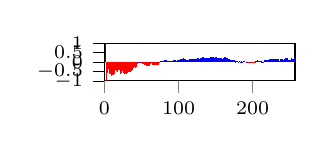
\begin{tikzpicture}

\definecolor{darkgray176}{RGB}{176,176,176}

\begin{axis}[
width=0.33\textwidth,
height=0.17\textwidth,
tick label style={font=\scriptsize},
tick align=outside,
tick pos=left,
xmin=0, xmax=257,
y grid style={darkgray176},
ymin=-1, ymax=1,
ytick style={color=black}
]
\draw[draw=none,fill=blue] (axis cs:0.6,0) rectangle (axis cs:1.4,4.43686862313796);
\draw[draw=none,fill=red] (axis cs:1.6,0) rectangle (axis cs:2.4,-2.53073250699069);
\draw[draw=none,fill=red] (axis cs:2.6,0) rectangle (axis cs:3.4,-0.544095144922911);
\draw[draw=none,fill=red] (axis cs:3.6,0) rectangle (axis cs:4.4,-0.59424428221722);
\draw[draw=none,fill=red] (axis cs:4.6,0) rectangle (axis cs:5.4,-0.394118283441539);
\draw[draw=none,fill=red] (axis cs:5.6,0) rectangle (axis cs:6.4,-0.639677150054839);
\draw[draw=none,fill=red] (axis cs:6.6,0) rectangle (axis cs:7.4,-0.564693162842682);
\draw[draw=none,fill=red] (axis cs:7.6,0) rectangle (axis cs:8.4,-0.659893355122916);
\draw[draw=none,fill=red] (axis cs:8.6,0) rectangle (axis cs:9.4,-0.732389581137625);
\draw[draw=none,fill=red] (axis cs:9.6,0) rectangle (axis cs:10.4,-0.37020775005067);
\draw[draw=none,fill=red] (axis cs:10.6,0) rectangle (axis cs:11.4,-0.676591169875821);
\draw[draw=none,fill=red] (axis cs:11.6,0) rectangle (axis cs:12.4,-0.70687685801627);
\draw[draw=none,fill=red] (axis cs:12.6,0) rectangle (axis cs:13.4,-0.6340383639621);
\draw[draw=none,fill=red] (axis cs:13.6,0) rectangle (axis cs:14.4,-0.567557248210878);
\draw[draw=none,fill=red] (axis cs:14.6,0) rectangle (axis cs:15.4,-0.418093593319502);
\draw[draw=none,fill=red] (axis cs:15.6,0) rectangle (axis cs:16.4,-0.453055465952281);
\draw[draw=none,fill=red] (axis cs:16.6,0) rectangle (axis cs:17.4,-0.554086375857379);
\draw[draw=none,fill=red] (axis cs:17.6,0) rectangle (axis cs:18.4,-0.528331805208143);
\draw[draw=none,fill=red] (axis cs:18.6,0) rectangle (axis cs:19.4,-0.412129838819974);
\draw[draw=none,fill=red] (axis cs:19.6,0) rectangle (axis cs:20.4,-0.413519580649401);
\draw[draw=none,fill=red] (axis cs:20.6,0) rectangle (axis cs:21.4,-0.657549470927206);
\draw[draw=none,fill=red] (axis cs:21.6,0) rectangle (axis cs:22.4,-0.626920174539054);
\draw[draw=none,fill=red] (axis cs:22.6,0) rectangle (axis cs:23.4,-0.588000738733083);
\draw[draw=none,fill=red] (axis cs:23.6,0) rectangle (axis cs:24.4,-0.48775367458461);
\draw[draw=none,fill=red] (axis cs:24.6,0) rectangle (axis cs:25.4,-0.489701648244108);
\draw[draw=none,fill=red] (axis cs:25.6,0) rectangle (axis cs:26.4,-0.59780970870703);
\draw[draw=none,fill=red] (axis cs:26.6,0) rectangle (axis cs:27.4,-0.626280498092185);
\draw[draw=none,fill=red] (axis cs:27.6,0) rectangle (axis cs:28.4,-0.639548871957337);
\draw[draw=none,fill=red] (axis cs:28.6,0) rectangle (axis cs:29.4,-0.541347460649877);
\draw[draw=none,fill=red] (axis cs:29.6,0) rectangle (axis cs:30.4,-0.626091842748878);
\draw[draw=none,fill=red] (axis cs:30.6,0) rectangle (axis cs:31.4,-0.560027379800219);
\draw[draw=none,fill=red] (axis cs:31.6,0) rectangle (axis cs:32.4,-0.530938296114721);
\draw[draw=none,fill=red] (axis cs:32.6,0) rectangle (axis cs:33.4,-0.532648619980997);
\draw[draw=none,fill=red] (axis cs:33.6,0) rectangle (axis cs:34.4,-0.537274198052277);
\draw[draw=none,fill=red] (axis cs:34.6,0) rectangle (axis cs:35.4,-0.524190596330788);
\draw[draw=none,fill=red] (axis cs:35.6,0) rectangle (axis cs:36.4,-0.454091423915034);
\draw[draw=none,fill=red] (axis cs:36.6,0) rectangle (axis cs:37.4,-0.420686115399353);
\draw[draw=none,fill=red] (axis cs:37.6,0) rectangle (axis cs:38.4,-0.347998389778352);
\draw[draw=none,fill=red] (axis cs:38.6,0) rectangle (axis cs:39.4,-0.32334237658289);
\draw[draw=none,fill=red] (axis cs:39.6,0) rectangle (axis cs:40.4,-0.273138043422107);
\draw[draw=none,fill=red] (axis cs:40.6,0) rectangle (axis cs:41.4,-0.317000326247493);
\draw[draw=none,fill=red] (axis cs:41.6,0) rectangle (axis cs:42.4,-0.187342168021042);
\draw[draw=none,fill=red] (axis cs:42.6,0) rectangle (axis cs:43.4,-0.241925881088349);
\draw[draw=none,fill=red] (axis cs:43.6,0) rectangle (axis cs:44.4,-0.123497637518194);
\draw[draw=none,fill=red] (axis cs:44.6,0) rectangle (axis cs:45.4,-0.124503583059174);
\draw[draw=none,fill=blue] (axis cs:45.6,0) rectangle (axis cs:46.4,0.00411681782433071);
\draw[draw=none,fill=blue] (axis cs:46.6,0) rectangle (axis cs:47.4,0.0107103966573057);
\draw[draw=none,fill=red] (axis cs:47.6,0) rectangle (axis cs:48.4,-0.000345477712761166);
\draw[draw=none,fill=red] (axis cs:48.6,0) rectangle (axis cs:49.4,-0.0230676765991751);
\draw[draw=none,fill=red] (axis cs:49.6,0) rectangle (axis cs:50.4,-0.016769554196272);
\draw[draw=none,fill=red] (axis cs:50.6,0) rectangle (axis cs:51.4,-0.109816221087022);
\draw[draw=none,fill=red] (axis cs:51.6,0) rectangle (axis cs:52.4,-0.119864502789084);
\draw[draw=none,fill=red] (axis cs:52.6,0) rectangle (axis cs:53.4,-0.111200848982664);
\draw[draw=none,fill=red] (axis cs:53.6,0) rectangle (axis cs:54.4,-0.161736337122676);
\draw[draw=none,fill=red] (axis cs:54.6,0) rectangle (axis cs:55.4,-0.166056332841474);
\draw[draw=none,fill=red] (axis cs:55.6,0) rectangle (axis cs:56.4,-0.163291043867608);
\draw[draw=none,fill=red] (axis cs:56.6,0) rectangle (axis cs:57.4,-0.207333568143968);
\draw[draw=none,fill=red] (axis cs:57.6,0) rectangle (axis cs:58.4,-0.211182970369717);
\draw[draw=none,fill=red] (axis cs:58.6,0) rectangle (axis cs:59.4,-0.218880236198958);
\draw[draw=none,fill=red] (axis cs:59.6,0) rectangle (axis cs:60.4,-0.216017078798298);
\draw[draw=none,fill=red] (axis cs:60.6,0) rectangle (axis cs:61.4,-0.199239530614228);
\draw[draw=none,fill=red] (axis cs:61.6,0) rectangle (axis cs:62.4,-0.111222017866637);
\draw[draw=none,fill=red] (axis cs:62.6,0) rectangle (axis cs:63.4,-0.0764668789610763);
\draw[draw=none,fill=red] (axis cs:63.6,0) rectangle (axis cs:64.4,-0.154502146954091);
\draw[draw=none,fill=red] (axis cs:64.6,0) rectangle (axis cs:65.4,-0.141373950725199);
\draw[draw=none,fill=red] (axis cs:65.6,0) rectangle (axis cs:66.4,-0.167575645484779);
\draw[draw=none,fill=red] (axis cs:66.6,0) rectangle (axis cs:67.4,-0.15281197452718);
\draw[draw=none,fill=red] (axis cs:67.6,0) rectangle (axis cs:68.4,-0.131456772094872);
\draw[draw=none,fill=red] (axis cs:68.6,0) rectangle (axis cs:69.4,-0.112817988091008);
\draw[draw=none,fill=red] (axis cs:69.6,0) rectangle (axis cs:70.4,-0.137824859378675);
\draw[draw=none,fill=red] (axis cs:70.6,0) rectangle (axis cs:71.4,-0.145444196712903);
\draw[draw=none,fill=red] (axis cs:71.6,0) rectangle (axis cs:72.4,-0.138412256262459);
\draw[draw=none,fill=red] (axis cs:72.6,0) rectangle (axis cs:73.4,-0.0461095045122661);
\draw[draw=none,fill=red] (axis cs:73.6,0) rectangle (axis cs:74.4,-0.03839968073616);
\draw[draw=none,fill=blue] (axis cs:74.6,0) rectangle (axis cs:75.4,0.0522285850824478);
\draw[draw=none,fill=blue] (axis cs:75.6,0) rectangle (axis cs:76.4,0.062377543645554);
\draw[draw=none,fill=blue] (axis cs:76.6,0) rectangle (axis cs:77.4,0.0574427022051864);
\draw[draw=none,fill=blue] (axis cs:77.6,0) rectangle (axis cs:78.4,0.0640909412040838);
\draw[draw=none,fill=blue] (axis cs:78.6,0) rectangle (axis cs:79.4,0.0489416044839723);
\draw[draw=none,fill=blue] (axis cs:79.6,0) rectangle (axis cs:80.4,0.0419875887880439);
\draw[draw=none,fill=blue] (axis cs:80.6,0) rectangle (axis cs:81.4,0.0891878585966941);
\draw[draw=none,fill=blue] (axis cs:81.6,0) rectangle (axis cs:82.4,0.0921702674507996);
\draw[draw=none,fill=blue] (axis cs:82.6,0) rectangle (axis cs:83.4,0.095762346380285);
\draw[draw=none,fill=blue] (axis cs:83.6,0) rectangle (axis cs:84.4,0.0882381889405064);
\draw[draw=none,fill=blue] (axis cs:84.6,0) rectangle (axis cs:85.4,0.0674520841912178);
\draw[draw=none,fill=blue] (axis cs:85.6,0) rectangle (axis cs:86.4,0.0479768704742032);
\draw[draw=none,fill=blue] (axis cs:86.6,0) rectangle (axis cs:87.4,0.0480542873725653);
\draw[draw=none,fill=blue] (axis cs:87.6,0) rectangle (axis cs:88.4,0.064936378829282);
\draw[draw=none,fill=blue] (axis cs:88.6,0) rectangle (axis cs:89.4,0.0577193765500006);
\draw[draw=none,fill=blue] (axis cs:89.6,0) rectangle (axis cs:90.4,0.0808665032107339);
\draw[draw=none,fill=blue] (axis cs:90.6,0) rectangle (axis cs:91.4,0.0763362457103405);
\draw[draw=none,fill=blue] (axis cs:91.6,0) rectangle (axis cs:92.4,0.0740949597955707);
\draw[draw=none,fill=blue] (axis cs:92.6,0) rectangle (axis cs:93.4,0.109438507441268);
\draw[draw=none,fill=blue] (axis cs:93.6,0) rectangle (axis cs:94.4,0.109349119560074);
\draw[draw=none,fill=blue] (axis cs:94.6,0) rectangle (axis cs:95.4,0.114410461986163);
\draw[draw=none,fill=blue] (axis cs:95.6,0) rectangle (axis cs:96.4,0.0697154237137578);
\draw[draw=none,fill=blue] (axis cs:96.6,0) rectangle (axis cs:97.4,0.0485191163330105);
\draw[draw=none,fill=blue] (axis cs:97.6,0) rectangle (axis cs:98.4,0.106453517107777);
\draw[draw=none,fill=blue] (axis cs:98.6,0) rectangle (axis cs:99.4,0.118408628556543);
\draw[draw=none,fill=blue] (axis cs:99.6,0) rectangle (axis cs:100.4,0.1154731654568);
\draw[draw=none,fill=blue] (axis cs:100.6,0) rectangle (axis cs:101.4,0.108864199992741);
\draw[draw=none,fill=blue] (axis cs:101.6,0) rectangle (axis cs:102.4,0.122895113763678);
\draw[draw=none,fill=blue] (axis cs:102.6,0) rectangle (axis cs:103.4,0.15148956850533);
\draw[draw=none,fill=blue] (axis cs:103.6,0) rectangle (axis cs:104.4,0.159173322717174);
\draw[draw=none,fill=blue] (axis cs:104.6,0) rectangle (axis cs:105.4,0.178525021679738);
\draw[draw=none,fill=blue] (axis cs:105.6,0) rectangle (axis cs:106.4,0.172089788848509);
\draw[draw=none,fill=blue] (axis cs:106.6,0) rectangle (axis cs:107.4,0.191888268666071);
\draw[draw=none,fill=blue] (axis cs:107.6,0) rectangle (axis cs:108.4,0.176253094043684);
\draw[draw=none,fill=blue] (axis cs:108.6,0) rectangle (axis cs:109.4,0.179747087159246);
\draw[draw=none,fill=blue] (axis cs:109.6,0) rectangle (axis cs:110.4,0.126382412828133);
\draw[draw=none,fill=blue] (axis cs:110.6,0) rectangle (axis cs:111.4,0.111831895325762);
\draw[draw=none,fill=blue] (axis cs:111.6,0) rectangle (axis cs:112.4,0.115491266278206);
\draw[draw=none,fill=blue] (axis cs:112.6,0) rectangle (axis cs:113.4,0.132713067899424);
\draw[draw=none,fill=blue] (axis cs:113.6,0) rectangle (axis cs:114.4,0.143976600384909);
\draw[draw=none,fill=blue] (axis cs:114.6,0) rectangle (axis cs:115.4,0.144119279338887);
\draw[draw=none,fill=blue] (axis cs:115.6,0) rectangle (axis cs:116.4,0.147591948780071);
\draw[draw=none,fill=blue] (axis cs:116.6,0) rectangle (axis cs:117.4,0.174340748680188);
\draw[draw=none,fill=blue] (axis cs:117.6,0) rectangle (axis cs:118.4,0.184286585528189);
\draw[draw=none,fill=blue] (axis cs:118.6,0) rectangle (axis cs:119.4,0.17402107306647);
\draw[draw=none,fill=blue] (axis cs:119.6,0) rectangle (axis cs:120.4,0.161222421451872);
\draw[draw=none,fill=blue] (axis cs:120.6,0) rectangle (axis cs:121.4,0.159838625854189);
\draw[draw=none,fill=blue] (axis cs:121.6,0) rectangle (axis cs:122.4,0.179744303807582);
\draw[draw=none,fill=blue] (axis cs:122.6,0) rectangle (axis cs:123.4,0.1851896922488);
\draw[draw=none,fill=blue] (axis cs:123.6,0) rectangle (axis cs:124.4,0.174986131243309);
\draw[draw=none,fill=blue] (axis cs:124.6,0) rectangle (axis cs:125.4,0.188958660756906);
\draw[draw=none,fill=blue] (axis cs:125.6,0) rectangle (axis cs:126.4,0.187926005474424);
\draw[draw=none,fill=blue] (axis cs:126.6,0) rectangle (axis cs:127.4,0.164832088146517);
\draw[draw=none,fill=blue] (axis cs:127.6,0) rectangle (axis cs:128.4,0.173588659078584);
\draw[draw=none,fill=blue] (axis cs:128.6,0) rectangle (axis cs:129.4,0.203671781104579);
\draw[draw=none,fill=blue] (axis cs:129.6,0) rectangle (axis cs:130.4,0.226923800449168);
\draw[draw=none,fill=blue] (axis cs:130.6,0) rectangle (axis cs:131.4,0.238066445715672);
\draw[draw=none,fill=blue] (axis cs:131.6,0) rectangle (axis cs:132.4,0.241095148713357);
\draw[draw=none,fill=blue] (axis cs:132.6,0) rectangle (axis cs:133.4,0.239485724448413);
\draw[draw=none,fill=blue] (axis cs:133.6,0) rectangle (axis cs:134.4,0.242591435409196);
\draw[draw=none,fill=blue] (axis cs:134.6,0) rectangle (axis cs:135.4,0.230161669398831);
\draw[draw=none,fill=blue] (axis cs:135.6,0) rectangle (axis cs:136.4,0.199547995278252);
\draw[draw=none,fill=blue] (axis cs:136.6,0) rectangle (axis cs:137.4,0.191006253959253);
\draw[draw=none,fill=blue] (axis cs:137.6,0) rectangle (axis cs:138.4,0.185232996449591);
\draw[draw=none,fill=blue] (axis cs:138.6,0) rectangle (axis cs:139.4,0.202928695653551);
\draw[draw=none,fill=blue] (axis cs:139.6,0) rectangle (axis cs:140.4,0.203692808702423);
\draw[draw=none,fill=blue] (axis cs:140.6,0) rectangle (axis cs:141.4,0.22399299748252);
\draw[draw=none,fill=blue] (axis cs:141.6,0) rectangle (axis cs:142.4,0.229522891722169);
\draw[draw=none,fill=blue] (axis cs:142.6,0) rectangle (axis cs:143.4,0.245845149489367);
\draw[draw=none,fill=blue] (axis cs:143.6,0) rectangle (axis cs:144.4,0.254704536410704);
\draw[draw=none,fill=blue] (axis cs:144.6,0) rectangle (axis cs:145.4,0.24811428172359);
\draw[draw=none,fill=blue] (axis cs:145.6,0) rectangle (axis cs:146.4,0.271701716354078);
\draw[draw=none,fill=blue] (axis cs:146.6,0) rectangle (axis cs:147.4,0.248683360194929);
\draw[draw=none,fill=blue] (axis cs:147.6,0) rectangle (axis cs:148.4,0.23337375006122);
\draw[draw=none,fill=blue] (axis cs:148.6,0) rectangle (axis cs:149.4,0.271533273597082);
\draw[draw=none,fill=blue] (axis cs:149.6,0) rectangle (axis cs:150.4,0.266069215098732);
\draw[draw=none,fill=blue] (axis cs:150.6,0) rectangle (axis cs:151.4,0.248198619766861);
\draw[draw=none,fill=blue] (axis cs:151.6,0) rectangle (axis cs:152.4,0.2321844846054);
\draw[draw=none,fill=blue] (axis cs:152.6,0) rectangle (axis cs:153.4,0.202078934248454);
\draw[draw=none,fill=blue] (axis cs:153.6,0) rectangle (axis cs:154.4,0.208729623533278);
\draw[draw=none,fill=blue] (axis cs:154.6,0) rectangle (axis cs:155.4,0.198110996334646);
\draw[draw=none,fill=blue] (axis cs:155.6,0) rectangle (axis cs:156.4,0.198129523150789);
\draw[draw=none,fill=blue] (axis cs:156.6,0) rectangle (axis cs:157.4,0.203591013703411);
\draw[draw=none,fill=blue] (axis cs:157.6,0) rectangle (axis cs:158.4,0.19439388486221);
\draw[draw=none,fill=blue] (axis cs:158.6,0) rectangle (axis cs:159.4,0.186650667210646);
\draw[draw=none,fill=blue] (axis cs:159.6,0) rectangle (axis cs:160.4,0.214585427899332);
\draw[draw=none,fill=blue] (axis cs:160.6,0) rectangle (axis cs:161.4,0.220023108825628);
\draw[draw=none,fill=blue] (axis cs:161.6,0) rectangle (axis cs:162.4,0.243240285371509);
\draw[draw=none,fill=blue] (axis cs:162.6,0) rectangle (axis cs:163.4,0.247349942037537);
\draw[draw=none,fill=blue] (axis cs:163.6,0) rectangle (axis cs:164.4,0.212105583548754);
\draw[draw=none,fill=blue] (axis cs:164.6,0) rectangle (axis cs:165.4,0.20093542344088);
\draw[draw=none,fill=blue] (axis cs:165.6,0) rectangle (axis cs:166.4,0.197099355508252);
\draw[draw=none,fill=blue] (axis cs:166.6,0) rectangle (axis cs:167.4,0.148065644195194);
\draw[draw=none,fill=blue] (axis cs:167.6,0) rectangle (axis cs:168.4,0.146748831813388);
\draw[draw=none,fill=blue] (axis cs:168.6,0) rectangle (axis cs:169.4,0.144672738152464);
\draw[draw=none,fill=blue] (axis cs:169.6,0) rectangle (axis cs:170.4,0.119103168960776);
\draw[draw=none,fill=blue] (axis cs:170.6,0) rectangle (axis cs:171.4,0.113820980361901);
\draw[draw=none,fill=blue] (axis cs:171.6,0) rectangle (axis cs:172.4,0.0912871696519413);
\draw[draw=none,fill=blue] (axis cs:172.6,0) rectangle (axis cs:173.4,0.0964009853543);
\draw[draw=none,fill=blue] (axis cs:173.6,0) rectangle (axis cs:174.4,0.102105076771348);
\draw[draw=none,fill=blue] (axis cs:174.6,0) rectangle (axis cs:175.4,0.0916675431398724);
\draw[draw=none,fill=blue] (axis cs:175.6,0) rectangle (axis cs:176.4,0.0625594485769958);
\draw[draw=none,fill=blue] (axis cs:176.6,0) rectangle (axis cs:177.4,0.0265716228759518);
\draw[draw=none,fill=blue] (axis cs:177.6,0) rectangle (axis cs:178.4,0.0356892786134386);
\draw[draw=none,fill=blue] (axis cs:178.6,0) rectangle (axis cs:179.4,0.0457970767264819);
\draw[draw=none,fill=blue] (axis cs:179.6,0) rectangle (axis cs:180.4,0.0261004199078765);
\draw[draw=none,fill=blue] (axis cs:180.6,0) rectangle (axis cs:181.4,0.0272092444631338);
\draw[draw=none,fill=blue] (axis cs:181.6,0) rectangle (axis cs:182.4,0.0342869859642256);
\draw[draw=none,fill=blue] (axis cs:182.6,0) rectangle (axis cs:183.4,0.0197510277844817);
\draw[draw=none,fill=blue] (axis cs:183.6,0) rectangle (axis cs:184.4,0.0197620729845496);
\draw[draw=none,fill=blue] (axis cs:184.6,0) rectangle (axis cs:185.4,0.0350966470619847);
\draw[draw=none,fill=blue] (axis cs:185.6,0) rectangle (axis cs:186.4,0.0233391153274156);
\draw[draw=none,fill=blue] (axis cs:186.6,0) rectangle (axis cs:187.4,0.0368371087262918);
\draw[draw=none,fill=blue] (axis cs:187.6,0) rectangle (axis cs:188.4,0.041867099628905);
\draw[draw=none,fill=blue] (axis cs:188.6,0) rectangle (axis cs:189.4,0.0418932135256962);
\draw[draw=none,fill=blue] (axis cs:189.6,0) rectangle (axis cs:190.4,0.000325531760135611);
\draw[draw=none,fill=blue] (axis cs:190.6,0) rectangle (axis cs:191.4,0.0171748664710343);
\draw[draw=none,fill=blue] (axis cs:191.6,0) rectangle (axis cs:192.4,0.00751212530310985);
\draw[draw=none,fill=blue] (axis cs:192.6,0) rectangle (axis cs:193.4,0.00617172284992717);
\draw[draw=none,fill=red] (axis cs:193.6,0) rectangle (axis cs:194.4,-0.00775449452912813);
\draw[draw=none,fill=red] (axis cs:194.6,0) rectangle (axis cs:195.4,-0.00968979422650751);
\draw[draw=none,fill=blue] (axis cs:195.6,0) rectangle (axis cs:196.4,0.00370480411283003);
\draw[draw=none,fill=red] (axis cs:196.6,0) rectangle (axis cs:197.4,-0.0278436212949078);
\draw[draw=none,fill=red] (axis cs:197.6,0) rectangle (axis cs:198.4,-0.0148359594356173);
\draw[draw=none,fill=red] (axis cs:198.6,0) rectangle (axis cs:199.4,-0.0158141390254762);
\draw[draw=none,fill=red] (axis cs:199.6,0) rectangle (axis cs:200.4,-0.0260654646182457);
\draw[draw=none,fill=red] (axis cs:200.6,0) rectangle (axis cs:201.4,-0.0156970250327406);
\draw[draw=none,fill=red] (axis cs:201.6,0) rectangle (axis cs:202.4,-0.00590459571081992);
\draw[draw=none,fill=red] (axis cs:202.6,0) rectangle (axis cs:203.4,-0.00507330292914121);
\draw[draw=none,fill=blue] (axis cs:203.6,0) rectangle (axis cs:204.4,0.0565254592638644);
\draw[draw=none,fill=blue] (axis cs:204.6,0) rectangle (axis cs:205.4,0.0564062676903041);
\draw[draw=none,fill=blue] (axis cs:205.6,0) rectangle (axis cs:206.4,0.0815522932353936);
\draw[draw=none,fill=blue] (axis cs:206.6,0) rectangle (axis cs:207.4,0.0682841717052911);
\draw[draw=none,fill=blue] (axis cs:207.6,0) rectangle (axis cs:208.4,0.0435200070754997);
\draw[draw=none,fill=blue] (axis cs:208.6,0) rectangle (axis cs:209.4,0.0421504112891111);
\draw[draw=none,fill=blue] (axis cs:209.6,0) rectangle (axis cs:210.4,0.0412626452605851);
\draw[draw=none,fill=blue] (axis cs:210.6,0) rectangle (axis cs:211.4,0.0192959417313903);
\draw[draw=none,fill=blue] (axis cs:211.6,0) rectangle (axis cs:212.4,0.0388356868424529);
\draw[draw=none,fill=blue] (axis cs:212.6,0) rectangle (axis cs:213.4,0.0269950054209707);
\draw[draw=none,fill=red] (axis cs:213.6,0) rectangle (axis cs:214.4,-0.0132777692691022);
\draw[draw=none,fill=blue] (axis cs:214.6,0) rectangle (axis cs:215.4,0.0561897738992161);
\draw[draw=none,fill=blue] (axis cs:215.6,0) rectangle (axis cs:216.4,0.0910069503963058);
\draw[draw=none,fill=blue] (axis cs:216.6,0) rectangle (axis cs:217.4,0.100220065334848);
\draw[draw=none,fill=blue] (axis cs:217.6,0) rectangle (axis cs:218.4,0.110894963112528);
\draw[draw=none,fill=blue] (axis cs:218.6,0) rectangle (axis cs:219.4,0.119828047502796);
\draw[draw=none,fill=blue] (axis cs:219.6,0) rectangle (axis cs:220.4,0.119263758955313);
\draw[draw=none,fill=blue] (axis cs:220.6,0) rectangle (axis cs:221.4,0.0989692944576896);
\draw[draw=none,fill=blue] (axis cs:221.6,0) rectangle (axis cs:222.4,0.10148659337508);
\draw[draw=none,fill=blue] (axis cs:222.6,0) rectangle (axis cs:223.4,0.153643460151352);
\draw[draw=none,fill=blue] (axis cs:223.6,0) rectangle (axis cs:224.4,0.146274770556305);
\draw[draw=none,fill=blue] (axis cs:224.6,0) rectangle (axis cs:225.4,0.147020852816961);
\draw[draw=none,fill=blue] (axis cs:225.6,0) rectangle (axis cs:226.4,0.147651402243076);
\draw[draw=none,fill=blue] (axis cs:226.6,0) rectangle (axis cs:227.4,0.160568392446856);
\draw[draw=none,fill=blue] (axis cs:227.6,0) rectangle (axis cs:228.4,0.181876570904459);
\draw[draw=none,fill=blue] (axis cs:228.6,0) rectangle (axis cs:229.4,0.174540586613313);
\draw[draw=none,fill=blue] (axis cs:229.6,0) rectangle (axis cs:230.4,0.169175336447893);
\draw[draw=none,fill=blue] (axis cs:230.6,0) rectangle (axis cs:231.4,0.161107578618277);
\draw[draw=none,fill=blue] (axis cs:231.6,0) rectangle (axis cs:232.4,0.180379813045894);
\draw[draw=none,fill=blue] (axis cs:232.6,0) rectangle (axis cs:233.4,0.157834408072995);
\draw[draw=none,fill=blue] (axis cs:233.6,0) rectangle (axis cs:234.4,0.151013686068773);
\draw[draw=none,fill=blue] (axis cs:234.6,0) rectangle (axis cs:235.4,0.0751719842196477);
\draw[draw=none,fill=blue] (axis cs:235.6,0) rectangle (axis cs:236.4,0.0653396598174352);
\draw[draw=none,fill=blue] (axis cs:236.6,0) rectangle (axis cs:237.4,0.173481077262926);
\draw[draw=none,fill=blue] (axis cs:237.6,0) rectangle (axis cs:238.4,0.134022485989321);
\draw[draw=none,fill=blue] (axis cs:238.6,0) rectangle (axis cs:239.4,0.140095274504896);
\draw[draw=none,fill=blue] (axis cs:239.6,0) rectangle (axis cs:240.4,0.144726498040398);
\draw[draw=none,fill=blue] (axis cs:240.6,0) rectangle (axis cs:241.4,0.124105849996215);
\draw[draw=none,fill=blue] (axis cs:241.6,0) rectangle (axis cs:242.4,0.137971202590384);
\draw[draw=none,fill=blue] (axis cs:242.6,0) rectangle (axis cs:243.4,0.113319841145204);
\draw[draw=none,fill=blue] (axis cs:243.6,0) rectangle (axis cs:244.4,0.216814850604521);
\draw[draw=none,fill=blue] (axis cs:244.6,0) rectangle (axis cs:245.4,0.194202468457136);
\draw[draw=none,fill=blue] (axis cs:245.6,0) rectangle (axis cs:246.4,0.196541190015819);
\draw[draw=none,fill=blue] (axis cs:246.6,0) rectangle (axis cs:247.4,0.156560502727829);
\draw[draw=none,fill=blue] (axis cs:247.6,0) rectangle (axis cs:248.4,0.103396771050175);
\draw[draw=none,fill=blue] (axis cs:248.6,0) rectangle (axis cs:249.4,0.102600961567372);
\draw[draw=none,fill=blue] (axis cs:249.6,0) rectangle (axis cs:250.4,0.0958989979737732);
\draw[draw=none,fill=blue] (axis cs:250.6,0) rectangle (axis cs:251.4,0.0821579293633397);
\draw[draw=none,fill=blue] (axis cs:251.6,0) rectangle (axis cs:252.4,0.217357548099795);
\draw[draw=none,fill=blue] (axis cs:252.6,0) rectangle (axis cs:253.4,0.177958514200572);
\draw[draw=none,fill=blue] (axis cs:253.6,0) rectangle (axis cs:254.4,0.165642110907581);
\draw[draw=none,fill=blue] (axis cs:254.6,0) rectangle (axis cs:255.4,0.148463196035141);
\draw[draw=none,fill=blue] (axis cs:255.6,0) rectangle (axis cs:256.4,0.22934355498086);
\end{axis}

\end{tikzpicture}

        \caption{SHAP values of UniAD}
        \label{fig:shap_uniad}
    \end{subfigure}
    \begin{subfigure}{1\linewidth}
        \centering
        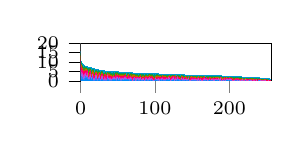
\begin{tikzpicture}

\definecolor{chocolate1961050}{RGB}{196,105,0}
\definecolor{crimson255078}{RGB}{255,0,78}
\definecolor{darkgray153}{RGB}{153,153,153}
\definecolor{darkslategray38}{RGB}{38,38,38}
\definecolor{darkslategray51}{RGB}{51,51,51}
\definecolor{darkturquoise0155207}{RGB}{0,155,207}
\definecolor{deeppink2510138}{RGB}{251,0,138}
\definecolor{dodgerblue0138250}{RGB}{0,138,250}
\definecolor{lightgray204}{RGB}{204,204,204}
\definecolor{mediumorchid21958191}{RGB}{219,58,191}
\definecolor{mediumpurple16495229}{RGB}{164,95,229}
\definecolor{olivedrab851440}{RGB}{85,144,0}
\definecolor{royalblue60122251}{RGB}{60,122,251}
\definecolor{teal015699}{RGB}{0,156,99}

\begin{axis}[
width=0.33\textwidth,
height=0.17\textwidth,
tick label style={font=\scriptsize},
tick align=outside,
tick pos=left,
xmin=0, xmax=256,
y grid style={darkgray176},
ymin=0, ymax=20,
ytick style={color=black},
ytick={0,5,10,15,20},
]
\addplot [semithick, darkgray153, forget plot]
table {%
0 4.44089209850063e-16
0 20
};
\draw[draw=none,fill=dodgerblue0138250] (axis cs:-0.35,0) rectangle (axis cs:0.35,3.56055124077294);

\draw[draw=none,fill=dodgerblue0138250] (axis cs:0.65,0) rectangle (axis cs:1.35,1.029204124882);
\draw[draw=none,fill=dodgerblue0138250] (axis cs:1.65,0) rectangle (axis cs:2.35,0.858598920252022);
\draw[draw=none,fill=dodgerblue0138250] (axis cs:2.65,0) rectangle (axis cs:3.35,0.941949664868445);
\draw[draw=none,fill=dodgerblue0138250] (axis cs:3.65,0) rectangle (axis cs:4.35,1.06252176754847);
\draw[draw=none,fill=dodgerblue0138250] (axis cs:4.65,0) rectangle (axis cs:5.35,0.361037976765911);
\draw[draw=none,fill=dodgerblue0138250] (axis cs:5.65,0) rectangle (axis cs:6.35,1.30357809847133);
\draw[draw=none,fill=dodgerblue0138250] (axis cs:6.65,0) rectangle (axis cs:7.35,1.79630065402632);
\draw[draw=none,fill=dodgerblue0138250] (axis cs:7.65,0) rectangle (axis cs:8.35,1.78265441138987);
\draw[draw=none,fill=dodgerblue0138250] (axis cs:8.65,0) rectangle (axis cs:9.35,1.15057253377889);
\draw[draw=none,fill=dodgerblue0138250] (axis cs:9.65,0) rectangle (axis cs:10.35,0.417015471945193);
\draw[draw=none,fill=dodgerblue0138250] (axis cs:10.65,0) rectangle (axis cs:11.35,0.673826335628655);
\draw[draw=none,fill=dodgerblue0138250] (axis cs:11.65,0) rectangle (axis cs:12.35,0.619923266137861);
\draw[draw=none,fill=dodgerblue0138250] (axis cs:12.65,0) rectangle (axis cs:13.35,1.32170248917266);
\draw[draw=none,fill=dodgerblue0138250] (axis cs:13.65,0) rectangle (axis cs:14.35,0.322413319361739);
\draw[draw=none,fill=dodgerblue0138250] (axis cs:14.65,0) rectangle (axis cs:15.35,0.579165791807319);
\draw[draw=none,fill=dodgerblue0138250] (axis cs:15.65,0) rectangle (axis cs:16.35,1.29326024765456);
\draw[draw=none,fill=dodgerblue0138250] (axis cs:16.65,0) rectangle (axis cs:17.35,0.387860952700959);
\draw[draw=none,fill=dodgerblue0138250] (axis cs:17.65,0) rectangle (axis cs:18.35,0.879669017765312);
\draw[draw=none,fill=dodgerblue0138250] (axis cs:18.65,0) rectangle (axis cs:19.35,0.216285793682312);
\draw[draw=none,fill=dodgerblue0138250] (axis cs:19.65,0) rectangle (axis cs:20.35,0.632448269487026);
\draw[draw=none,fill=dodgerblue0138250] (axis cs:20.65,0) rectangle (axis cs:21.35,0.673255475023874);
\draw[draw=none,fill=dodgerblue0138250] (axis cs:21.65,0) rectangle (axis cs:22.35,0.273392295779842);
\draw[draw=none,fill=dodgerblue0138250] (axis cs:22.65,0) rectangle (axis cs:23.35,0.298563539124294);
\draw[draw=none,fill=dodgerblue0138250] (axis cs:23.65,0) rectangle (axis cs:24.35,0.741049103139397);
\draw[draw=none,fill=dodgerblue0138250] (axis cs:24.65,0) rectangle (axis cs:25.35,0.730514865466308);
\draw[draw=none,fill=dodgerblue0138250] (axis cs:25.65,0) rectangle (axis cs:26.35,0.422391195890572);
\draw[draw=none,fill=dodgerblue0138250] (axis cs:26.65,0) rectangle (axis cs:27.35,0.211733400271512);
\draw[draw=none,fill=dodgerblue0138250] (axis cs:27.65,0) rectangle (axis cs:28.35,0.577139494758931);
\draw[draw=none,fill=dodgerblue0138250] (axis cs:28.65,0) rectangle (axis cs:29.35,0.440165748879186);
\draw[draw=none,fill=dodgerblue0138250] (axis cs:29.65,0) rectangle (axis cs:30.35,0.27232673108812);
\draw[draw=none,fill=dodgerblue0138250] (axis cs:30.65,0) rectangle (axis cs:31.35,0.478799694628495);
\draw[draw=none,fill=dodgerblue0138250] (axis cs:31.65,0) rectangle (axis cs:32.35,0.265442747829211);
\draw[draw=none,fill=dodgerblue0138250] (axis cs:32.65,0) rectangle (axis cs:33.35,0.464158901004634);
\draw[draw=none,fill=dodgerblue0138250] (axis cs:33.65,0) rectangle (axis cs:34.35,0.513622220328366);
\draw[draw=none,fill=dodgerblue0138250] (axis cs:34.65,0) rectangle (axis cs:35.35,0.50001495815034);
\draw[draw=none,fill=dodgerblue0138250] (axis cs:35.65,0) rectangle (axis cs:36.35,0.59797076280255);
\draw[draw=none,fill=dodgerblue0138250] (axis cs:36.65,0) rectangle (axis cs:37.35,0.45708866014028);
\draw[draw=none,fill=dodgerblue0138250] (axis cs:37.65,0) rectangle (axis cs:38.35,0.478303450682803);
\draw[draw=none,fill=dodgerblue0138250] (axis cs:38.65,0) rectangle (axis cs:39.35,0.182957045425262);
\draw[draw=none,fill=dodgerblue0138250] (axis cs:39.65,0) rectangle (axis cs:40.35,0.392519624879598);
\draw[draw=none,fill=dodgerblue0138250] (axis cs:40.65,0) rectangle (axis cs:41.35,0.209695151575466);
\draw[draw=none,fill=dodgerblue0138250] (axis cs:41.65,0) rectangle (axis cs:42.35,0.713732330497611);
\draw[draw=none,fill=dodgerblue0138250] (axis cs:42.65,0) rectangle (axis cs:43.35,0.915818572964813);
\draw[draw=none,fill=dodgerblue0138250] (axis cs:43.65,0) rectangle (axis cs:44.35,0.840234532268709);
\draw[draw=none,fill=dodgerblue0138250] (axis cs:44.65,0) rectangle (axis cs:45.35,0.257654788442476);
\draw[draw=none,fill=dodgerblue0138250] (axis cs:45.65,0) rectangle (axis cs:46.35,0.709642199411272);
\draw[draw=none,fill=dodgerblue0138250] (axis cs:46.65,0) rectangle (axis cs:47.35,1.02354655942063);
\draw[draw=none,fill=dodgerblue0138250] (axis cs:47.65,0) rectangle (axis cs:48.35,0.423905841413264);
\draw[draw=none,fill=dodgerblue0138250] (axis cs:48.65,0) rectangle (axis cs:49.35,1.00712973402212);
\draw[draw=none,fill=dodgerblue0138250] (axis cs:49.65,0) rectangle (axis cs:50.35,0.611563048951209);
\draw[draw=none,fill=dodgerblue0138250] (axis cs:50.65,0) rectangle (axis cs:51.35,0.667346685136471);
\draw[draw=none,fill=dodgerblue0138250] (axis cs:51.65,0) rectangle (axis cs:52.35,0.536655189330874);
\draw[draw=none,fill=dodgerblue0138250] (axis cs:52.65,0) rectangle (axis cs:53.35,0.199607838799549);
\draw[draw=none,fill=dodgerblue0138250] (axis cs:53.65,0) rectangle (axis cs:54.35,0.289015849946108);
\draw[draw=none,fill=dodgerblue0138250] (axis cs:54.65,0) rectangle (axis cs:55.35,0.384007919361916);
\draw[draw=none,fill=dodgerblue0138250] (axis cs:55.65,0) rectangle (axis cs:56.35,0.512388476074272);
\draw[draw=none,fill=dodgerblue0138250] (axis cs:56.65,0) rectangle (axis cs:57.35,0.587132756261963);
\draw[draw=none,fill=dodgerblue0138250] (axis cs:57.65,0) rectangle (axis cs:58.35,0.428500813334505);
\draw[draw=none,fill=dodgerblue0138250] (axis cs:58.65,0) rectangle (axis cs:59.35,0.451412619785783);
\draw[draw=none,fill=dodgerblue0138250] (axis cs:59.65,0) rectangle (axis cs:60.35,0.51826883408023);
\draw[draw=none,fill=dodgerblue0138250] (axis cs:60.65,0) rectangle (axis cs:61.35,0.626866808387543);
\draw[draw=none,fill=dodgerblue0138250] (axis cs:61.65,0) rectangle (axis cs:62.35,0.272654143045519);
\draw[draw=none,fill=dodgerblue0138250] (axis cs:62.65,0) rectangle (axis cs:63.35,0.283919952216501);
\draw[draw=none,fill=dodgerblue0138250] (axis cs:63.65,0) rectangle (axis cs:64.35,0.305236573002288);
\draw[draw=none,fill=dodgerblue0138250] (axis cs:64.65,0) rectangle (axis cs:65.35,0.342853880640696);
\draw[draw=none,fill=dodgerblue0138250] (axis cs:65.65,0) rectangle (axis cs:66.35,0.173609121529028);
\draw[draw=none,fill=dodgerblue0138250] (axis cs:66.65,0) rectangle (axis cs:67.35,0.446106129428457);
\draw[draw=none,fill=dodgerblue0138250] (axis cs:67.65,0) rectangle (axis cs:68.35,0.498736599977507);
\draw[draw=none,fill=dodgerblue0138250] (axis cs:68.65,0) rectangle (axis cs:69.35,0.229731513799464);
\draw[draw=none,fill=dodgerblue0138250] (axis cs:69.65,0) rectangle (axis cs:70.35,0.458000644758029);
\draw[draw=none,fill=dodgerblue0138250] (axis cs:70.65,0) rectangle (axis cs:71.35,0.238339548330075);
\draw[draw=none,fill=dodgerblue0138250] (axis cs:71.65,0) rectangle (axis cs:72.35,0.331052947294016);
\draw[draw=none,fill=dodgerblue0138250] (axis cs:72.65,0) rectangle (axis cs:73.35,0.365991495760809);
\draw[draw=none,fill=dodgerblue0138250] (axis cs:73.65,0) rectangle (axis cs:74.35,0.213273742172343);
\draw[draw=none,fill=dodgerblue0138250] (axis cs:74.65,0) rectangle (axis cs:75.35,0.182184504882355);
\draw[draw=none,fill=dodgerblue0138250] (axis cs:75.65,0) rectangle (axis cs:76.35,0.661013296063667);
\draw[draw=none,fill=dodgerblue0138250] (axis cs:76.65,0) rectangle (axis cs:77.35,0.234762970741987);
\draw[draw=none,fill=dodgerblue0138250] (axis cs:77.65,0) rectangle (axis cs:78.35,0.260297842403247);
\draw[draw=none,fill=dodgerblue0138250] (axis cs:78.65,0) rectangle (axis cs:79.35,0.184076119268849);
\draw[draw=none,fill=dodgerblue0138250] (axis cs:79.65,0) rectangle (axis cs:80.35,0.323456680978019);
\draw[draw=none,fill=dodgerblue0138250] (axis cs:80.65,0) rectangle (axis cs:81.35,0.452103158743061);
\draw[draw=none,fill=dodgerblue0138250] (axis cs:81.65,0) rectangle (axis cs:82.35,0.369909914923939);
\draw[draw=none,fill=dodgerblue0138250] (axis cs:82.65,0) rectangle (axis cs:83.35,0.448073966407368);
\draw[draw=none,fill=dodgerblue0138250] (axis cs:83.65,0) rectangle (axis cs:84.35,0.254282676868328);
\draw[draw=none,fill=dodgerblue0138250] (axis cs:84.65,0) rectangle (axis cs:85.35,0.138951230410156);
\draw[draw=none,fill=dodgerblue0138250] (axis cs:85.65,0) rectangle (axis cs:86.35,0.336889904961495);
\draw[draw=none,fill=dodgerblue0138250] (axis cs:86.65,0) rectangle (axis cs:87.35,0.212707234712557);
\draw[draw=none,fill=dodgerblue0138250] (axis cs:87.65,0) rectangle (axis cs:88.35,0.353824422610542);
\draw[draw=none,fill=dodgerblue0138250] (axis cs:88.65,0) rectangle (axis cs:89.35,0.818201583804886);
\draw[draw=none,fill=dodgerblue0138250] (axis cs:89.65,0) rectangle (axis cs:90.35,0.418061898352838);
\draw[draw=none,fill=dodgerblue0138250] (axis cs:90.65,0) rectangle (axis cs:91.35,0.301227781228776);
\draw[draw=none,fill=dodgerblue0138250] (axis cs:91.65,0) rectangle (axis cs:92.35,0.28002051614031);
\draw[draw=none,fill=dodgerblue0138250] (axis cs:92.65,0) rectangle (axis cs:93.35,0.294110592921811);
\draw[draw=none,fill=dodgerblue0138250] (axis cs:93.65,0) rectangle (axis cs:94.35,0.511290049549411);
\draw[draw=none,fill=dodgerblue0138250] (axis cs:94.65,0) rectangle (axis cs:95.35,0.484831387296319);
\draw[draw=none,fill=dodgerblue0138250] (axis cs:95.65,0) rectangle (axis cs:96.35,0.200916285003143);
\draw[draw=none,fill=dodgerblue0138250] (axis cs:96.65,0) rectangle (axis cs:97.35,0.884580604248866);
\draw[draw=none,fill=dodgerblue0138250] (axis cs:97.65,0) rectangle (axis cs:98.35,0.163848739797372);
\draw[draw=none,fill=dodgerblue0138250] (axis cs:98.65,0) rectangle (axis cs:99.35,0.212882966569063);
\draw[draw=none,fill=dodgerblue0138250] (axis cs:99.65,0) rectangle (axis cs:100.35,0.527743271600133);
\draw[draw=none,fill=dodgerblue0138250] (axis cs:100.65,0) rectangle (axis cs:101.35,0.413764588678761);
\draw[draw=none,fill=dodgerblue0138250] (axis cs:101.65,0) rectangle (axis cs:102.35,0.226330506871062);
\draw[draw=none,fill=dodgerblue0138250] (axis cs:102.65,0) rectangle (axis cs:103.35,0.206685658805995);
\draw[draw=none,fill=dodgerblue0138250] (axis cs:103.65,0) rectangle (axis cs:104.35,0.203653746525951);
\draw[draw=none,fill=dodgerblue0138250] (axis cs:104.65,0) rectangle (axis cs:105.35,0.742296924207397);
\draw[draw=none,fill=dodgerblue0138250] (axis cs:105.65,0) rectangle (axis cs:106.35,0.15236661006997);
\draw[draw=none,fill=dodgerblue0138250] (axis cs:106.65,0) rectangle (axis cs:107.35,0.276842993295211);
\draw[draw=none,fill=dodgerblue0138250] (axis cs:107.65,0) rectangle (axis cs:108.35,0.289776845954695);
\draw[draw=none,fill=dodgerblue0138250] (axis cs:108.65,0) rectangle (axis cs:109.35,0.102668589678038);
\draw[draw=none,fill=dodgerblue0138250] (axis cs:109.65,0) rectangle (axis cs:110.35,0.404778345263015);
\draw[draw=none,fill=dodgerblue0138250] (axis cs:110.65,0) rectangle (axis cs:111.35,0.519232342010522);
\draw[draw=none,fill=dodgerblue0138250] (axis cs:111.65,0) rectangle (axis cs:112.35,0.364864940002102);
\draw[draw=none,fill=dodgerblue0138250] (axis cs:112.65,0) rectangle (axis cs:113.35,0.23289417278198);
\draw[draw=none,fill=dodgerblue0138250] (axis cs:113.65,0) rectangle (axis cs:114.35,0.393664880008648);
\draw[draw=none,fill=dodgerblue0138250] (axis cs:114.65,0) rectangle (axis cs:115.35,0.51505126149641);
\draw[draw=none,fill=dodgerblue0138250] (axis cs:115.65,0) rectangle (axis cs:116.35,0.544521331988259);
\draw[draw=none,fill=dodgerblue0138250] (axis cs:116.65,0) rectangle (axis cs:117.35,0.490863522246465);
\draw[draw=none,fill=dodgerblue0138250] (axis cs:117.65,0) rectangle (axis cs:118.35,0.29207861470664);
\draw[draw=none,fill=dodgerblue0138250] (axis cs:118.65,0) rectangle (axis cs:119.35,0.25293255093421);
\draw[draw=none,fill=dodgerblue0138250] (axis cs:119.65,0) rectangle (axis cs:120.35,0.459955958979592);
\draw[draw=none,fill=dodgerblue0138250] (axis cs:120.65,0) rectangle (axis cs:121.35,0.220043732299735);
\draw[draw=none,fill=dodgerblue0138250] (axis cs:121.65,0) rectangle (axis cs:122.35,0.153481920846427);
\draw[draw=none,fill=dodgerblue0138250] (axis cs:122.65,0) rectangle (axis cs:123.35,0.379500157985259);
\draw[draw=none,fill=dodgerblue0138250] (axis cs:123.65,0) rectangle (axis cs:124.35,0.574346508546655);
\draw[draw=none,fill=dodgerblue0138250] (axis cs:124.65,0) rectangle (axis cs:125.35,0.725878365999855);
\draw[draw=none,fill=dodgerblue0138250] (axis cs:125.65,0) rectangle (axis cs:126.35,0.321302301674422);
\draw[draw=none,fill=dodgerblue0138250] (axis cs:126.65,0) rectangle (axis cs:127.35,0.57879584899635);
\draw[draw=none,fill=dodgerblue0138250] (axis cs:127.65,0) rectangle (axis cs:128.35,0.406455925900216);
\draw[draw=none,fill=dodgerblue0138250] (axis cs:128.65,0) rectangle (axis cs:129.35,0.129558991353209);
\draw[draw=none,fill=dodgerblue0138250] (axis cs:129.65,0) rectangle (axis cs:130.35,0.416357732229188);
\draw[draw=none,fill=dodgerblue0138250] (axis cs:130.65,0) rectangle (axis cs:131.35,0.538694413600784);
\draw[draw=none,fill=dodgerblue0138250] (axis cs:131.65,0) rectangle (axis cs:132.35,0.245482090840214);
\draw[draw=none,fill=dodgerblue0138250] (axis cs:132.65,0) rectangle (axis cs:133.35,0.150840203096493);
\draw[draw=none,fill=dodgerblue0138250] (axis cs:133.65,0) rectangle (axis cs:134.35,0.355821062989914);
\draw[draw=none,fill=dodgerblue0138250] (axis cs:134.65,0) rectangle (axis cs:135.35,0.655472807037631);
\draw[draw=none,fill=dodgerblue0138250] (axis cs:135.65,0) rectangle (axis cs:136.35,0.429813643623941);
\draw[draw=none,fill=dodgerblue0138250] (axis cs:136.65,0) rectangle (axis cs:137.35,0.165423442811527);
\draw[draw=none,fill=dodgerblue0138250] (axis cs:137.65,0) rectangle (axis cs:138.35,0.384369812292426);
\draw[draw=none,fill=dodgerblue0138250] (axis cs:138.65,0) rectangle (axis cs:139.35,0.114147037938257);
\draw[draw=none,fill=dodgerblue0138250] (axis cs:139.65,0) rectangle (axis cs:140.35,0.353775549308723);
\draw[draw=none,fill=dodgerblue0138250] (axis cs:140.65,0) rectangle (axis cs:141.35,0.366412033735957);
\draw[draw=none,fill=dodgerblue0138250] (axis cs:141.65,0) rectangle (axis cs:142.35,0.475329284590404);
\draw[draw=none,fill=dodgerblue0138250] (axis cs:142.65,0) rectangle (axis cs:143.35,0.347099327634402);
\draw[draw=none,fill=dodgerblue0138250] (axis cs:143.65,0) rectangle (axis cs:144.35,0.266226438827594);
\draw[draw=none,fill=dodgerblue0138250] (axis cs:144.65,0) rectangle (axis cs:145.35,0.489265804067038);
\draw[draw=none,fill=dodgerblue0138250] (axis cs:145.65,0) rectangle (axis cs:146.35,0.203057258331633);
\draw[draw=none,fill=dodgerblue0138250] (axis cs:146.65,0) rectangle (axis cs:147.35,0.194161444827113);
\draw[draw=none,fill=dodgerblue0138250] (axis cs:147.65,0) rectangle (axis cs:148.35,0.286308013405996);
\draw[draw=none,fill=dodgerblue0138250] (axis cs:148.65,0) rectangle (axis cs:149.35,0.199153743144315);
\draw[draw=none,fill=dodgerblue0138250] (axis cs:149.65,0) rectangle (axis cs:150.35,0.275214587655992);
\draw[draw=none,fill=dodgerblue0138250] (axis cs:150.65,0) rectangle (axis cs:151.35,0.125177343952758);
\draw[draw=none,fill=dodgerblue0138250] (axis cs:151.65,0) rectangle (axis cs:152.35,0.927879534702646);
\draw[draw=none,fill=dodgerblue0138250] (axis cs:152.65,0) rectangle (axis cs:153.35,0.0995742167447263);
\draw[draw=none,fill=dodgerblue0138250] (axis cs:153.65,0) rectangle (axis cs:154.35,0.38341230764787);
\draw[draw=none,fill=dodgerblue0138250] (axis cs:154.65,0) rectangle (axis cs:155.35,0.238177720930775);
\draw[draw=none,fill=dodgerblue0138250] (axis cs:155.65,0) rectangle (axis cs:156.35,0.320912237540365);
\draw[draw=none,fill=dodgerblue0138250] (axis cs:156.65,0) rectangle (axis cs:157.35,0.113341955883851);
\draw[draw=none,fill=dodgerblue0138250] (axis cs:157.65,0) rectangle (axis cs:158.35,0.274266871103004);
\draw[draw=none,fill=dodgerblue0138250] (axis cs:158.65,0) rectangle (axis cs:159.35,0.395085436410091);
\draw[draw=none,fill=dodgerblue0138250] (axis cs:159.65,0) rectangle (axis cs:160.35,0.351105819426109);
\draw[draw=none,fill=dodgerblue0138250] (axis cs:160.65,0) rectangle (axis cs:161.35,0.237690414405747);
\draw[draw=none,fill=dodgerblue0138250] (axis cs:161.65,0) rectangle (axis cs:162.35,0.478742744945424);
\draw[draw=none,fill=dodgerblue0138250] (axis cs:162.65,0) rectangle (axis cs:163.35,0.170910094689756);
\draw[draw=none,fill=dodgerblue0138250] (axis cs:163.65,0) rectangle (axis cs:164.35,0.50282591102692);
\draw[draw=none,fill=dodgerblue0138250] (axis cs:164.65,0) rectangle (axis cs:165.35,0.253330902558101);
\draw[draw=none,fill=dodgerblue0138250] (axis cs:165.65,0) rectangle (axis cs:166.35,0.19982291102387);
\draw[draw=none,fill=dodgerblue0138250] (axis cs:166.65,0) rectangle (axis cs:167.35,0.299390011977855);
\draw[draw=none,fill=dodgerblue0138250] (axis cs:167.65,0) rectangle (axis cs:168.35,0.532439838688661);
\draw[draw=none,fill=dodgerblue0138250] (axis cs:168.65,0) rectangle (axis cs:169.35,0.407375495656632);
\draw[draw=none,fill=dodgerblue0138250] (axis cs:169.65,0) rectangle (axis cs:170.35,0.412798489678069);
\draw[draw=none,fill=dodgerblue0138250] (axis cs:170.65,0) rectangle (axis cs:171.35,0.322738804353898);
\draw[draw=none,fill=dodgerblue0138250] (axis cs:171.65,0) rectangle (axis cs:172.35,0.442429469437988);
\draw[draw=none,fill=dodgerblue0138250] (axis cs:172.65,0) rectangle (axis cs:173.35,0.519443059361526);
\draw[draw=none,fill=dodgerblue0138250] (axis cs:173.65,0) rectangle (axis cs:174.35,0.187965023060918);
\draw[draw=none,fill=dodgerblue0138250] (axis cs:174.65,0) rectangle (axis cs:175.35,0.186700957948897);
\draw[draw=none,fill=dodgerblue0138250] (axis cs:175.65,0) rectangle (axis cs:176.35,0.299037770817428);
\draw[draw=none,fill=dodgerblue0138250] (axis cs:176.65,0) rectangle (axis cs:177.35,0.311916537992459);
\draw[draw=none,fill=dodgerblue0138250] (axis cs:177.65,0) rectangle (axis cs:178.35,0.14534003963691);
\draw[draw=none,fill=dodgerblue0138250] (axis cs:178.65,0) rectangle (axis cs:179.35,0.146563704632893);
\draw[draw=none,fill=dodgerblue0138250] (axis cs:179.65,0) rectangle (axis cs:180.35,0.140125430213567);
\draw[draw=none,fill=dodgerblue0138250] (axis cs:180.65,0) rectangle (axis cs:181.35,0.37860845201468);
\draw[draw=none,fill=dodgerblue0138250] (axis cs:181.65,0) rectangle (axis cs:182.35,0.46509335456336);
\draw[draw=none,fill=dodgerblue0138250] (axis cs:182.65,0) rectangle (axis cs:183.35,0.334225969988758);
\draw[draw=none,fill=dodgerblue0138250] (axis cs:183.65,0) rectangle (axis cs:184.35,0.328688260064707);
\draw[draw=none,fill=dodgerblue0138250] (axis cs:184.65,0) rectangle (axis cs:185.35,0.506756274839709);
\draw[draw=none,fill=dodgerblue0138250] (axis cs:185.65,0) rectangle (axis cs:186.35,0.454567921024477);
\draw[draw=none,fill=dodgerblue0138250] (axis cs:186.65,0) rectangle (axis cs:187.35,0.292410964871353);
\draw[draw=none,fill=dodgerblue0138250] (axis cs:187.65,0) rectangle (axis cs:188.35,0.488069198166209);
\draw[draw=none,fill=dodgerblue0138250] (axis cs:188.65,0) rectangle (axis cs:189.35,0.153000164961209);
\draw[draw=none,fill=dodgerblue0138250] (axis cs:189.65,0) rectangle (axis cs:190.35,0.379762094220606);
\draw[draw=none,fill=dodgerblue0138250] (axis cs:190.65,0) rectangle (axis cs:191.35,0.305587740260394);
\draw[draw=none,fill=dodgerblue0138250] (axis cs:191.65,0) rectangle (axis cs:192.35,0.324239645333177);
\draw[draw=none,fill=dodgerblue0138250] (axis cs:192.65,0) rectangle (axis cs:193.35,0.421975597647725);
\draw[draw=none,fill=dodgerblue0138250] (axis cs:193.65,0) rectangle (axis cs:194.35,0.357161633349733);
\draw[draw=none,fill=dodgerblue0138250] (axis cs:194.65,0) rectangle (axis cs:195.35,0.225068615272102);
\draw[draw=none,fill=dodgerblue0138250] (axis cs:195.65,0) rectangle (axis cs:196.35,0.307761548086924);
\draw[draw=none,fill=dodgerblue0138250] (axis cs:196.65,0) rectangle (axis cs:197.35,0.312944186545891);
\draw[draw=none,fill=dodgerblue0138250] (axis cs:197.65,0) rectangle (axis cs:198.35,0.296299229594198);
\draw[draw=none,fill=dodgerblue0138250] (axis cs:198.65,0) rectangle (axis cs:199.35,0.0979036678367248);
\draw[draw=none,fill=dodgerblue0138250] (axis cs:199.65,0) rectangle (axis cs:200.35,0.475627398396145);
\draw[draw=none,fill=dodgerblue0138250] (axis cs:200.65,0) rectangle (axis cs:201.35,0.305063462170454);
\draw[draw=none,fill=dodgerblue0138250] (axis cs:201.65,0) rectangle (axis cs:202.35,0.323548889645904);
\draw[draw=none,fill=dodgerblue0138250] (axis cs:202.65,0) rectangle (axis cs:203.35,0.312398911672242);
\draw[draw=none,fill=dodgerblue0138250] (axis cs:203.65,0) rectangle (axis cs:204.35,0.12912472594524);
\draw[draw=none,fill=dodgerblue0138250] (axis cs:204.65,0) rectangle (axis cs:205.35,0.224600072222139);
\draw[draw=none,fill=dodgerblue0138250] (axis cs:205.65,0) rectangle (axis cs:206.35,0.208218000838014);
\draw[draw=none,fill=dodgerblue0138250] (axis cs:206.65,0) rectangle (axis cs:207.35,0.231714823387475);
\draw[draw=none,fill=dodgerblue0138250] (axis cs:207.65,0) rectangle (axis cs:208.35,0.236396469774128);
\draw[draw=none,fill=dodgerblue0138250] (axis cs:208.65,0) rectangle (axis cs:209.35,0.160406060235415);
\draw[draw=none,fill=dodgerblue0138250] (axis cs:209.65,0) rectangle (axis cs:210.35,0.154778154117987);
\draw[draw=none,fill=dodgerblue0138250] (axis cs:210.65,0) rectangle (axis cs:211.35,0.314236108697708);
\draw[draw=none,fill=dodgerblue0138250] (axis cs:211.65,0) rectangle (axis cs:212.35,0.3530058654995);
\draw[draw=none,fill=dodgerblue0138250] (axis cs:212.65,0) rectangle (axis cs:213.35,0.142859980584725);
\draw[draw=none,fill=dodgerblue0138250] (axis cs:213.65,0) rectangle (axis cs:214.35,0.0899623794750926);
\draw[draw=none,fill=dodgerblue0138250] (axis cs:214.65,0) rectangle (axis cs:215.35,0.130744231287081);
\draw[draw=none,fill=dodgerblue0138250] (axis cs:215.65,0) rectangle (axis cs:216.35,0.159018159667414);
\draw[draw=none,fill=dodgerblue0138250] (axis cs:216.65,0) rectangle (axis cs:217.35,0.323771272339566);
\draw[draw=none,fill=dodgerblue0138250] (axis cs:217.65,0) rectangle (axis cs:218.35,0.242427142188319);
\draw[draw=none,fill=dodgerblue0138250] (axis cs:218.65,0) rectangle (axis cs:219.35,0.117955495636067);
\draw[draw=none,fill=dodgerblue0138250] (axis cs:219.65,0) rectangle (axis cs:220.35,0.322394425712958);
\draw[draw=none,fill=dodgerblue0138250] (axis cs:220.65,0) rectangle (axis cs:221.35,0.106494130098587);
\draw[draw=none,fill=dodgerblue0138250] (axis cs:221.65,0) rectangle (axis cs:222.35,0.196252911109516);
\draw[draw=none,fill=dodgerblue0138250] (axis cs:222.65,0) rectangle (axis cs:223.35,0.176467624634895);
\draw[draw=none,fill=dodgerblue0138250] (axis cs:223.65,0) rectangle (axis cs:224.35,0.172134732383401);
\draw[draw=none,fill=dodgerblue0138250] (axis cs:224.65,0) rectangle (axis cs:225.35,0.09880296417793);
\draw[draw=none,fill=dodgerblue0138250] (axis cs:225.65,0) rectangle (axis cs:226.35,0.304707233198047);
\draw[draw=none,fill=dodgerblue0138250] (axis cs:226.65,0) rectangle (axis cs:227.35,0.32631317820831);
\draw[draw=none,fill=dodgerblue0138250] (axis cs:227.65,0) rectangle (axis cs:228.35,0.0962885849955357);
\draw[draw=none,fill=dodgerblue0138250] (axis cs:228.65,0) rectangle (axis cs:229.35,0.160764851717274);
\draw[draw=none,fill=dodgerblue0138250] (axis cs:229.65,0) rectangle (axis cs:230.35,0.270872418407304);
\draw[draw=none,fill=dodgerblue0138250] (axis cs:230.65,0) rectangle (axis cs:231.35,0.182105184533499);
\draw[draw=none,fill=dodgerblue0138250] (axis cs:231.65,0) rectangle (axis cs:232.35,0.15601788920565);
\draw[draw=none,fill=dodgerblue0138250] (axis cs:232.65,0) rectangle (axis cs:233.35,0.154265156929177);
\draw[draw=none,fill=dodgerblue0138250] (axis cs:233.65,0) rectangle (axis cs:234.35,0.239497744832646);
\draw[draw=none,fill=dodgerblue0138250] (axis cs:234.65,0) rectangle (axis cs:235.35,0.124119138891723);
\draw[draw=none,fill=dodgerblue0138250] (axis cs:235.65,0) rectangle (axis cs:236.35,0.197167954620356);
\draw[draw=none,fill=dodgerblue0138250] (axis cs:236.65,0) rectangle (axis cs:237.35,0.0899784946855559);
\draw[draw=none,fill=dodgerblue0138250] (axis cs:237.65,0) rectangle (axis cs:238.35,0.122665553429604);
\draw[draw=none,fill=dodgerblue0138250] (axis cs:238.65,0) rectangle (axis cs:239.35,0.121209782134316);
\draw[draw=none,fill=dodgerblue0138250] (axis cs:239.65,0) rectangle (axis cs:240.35,0.177928234603617);
\draw[draw=none,fill=dodgerblue0138250] (axis cs:240.65,0) rectangle (axis cs:241.35,0.182632048904107);
\draw[draw=none,fill=dodgerblue0138250] (axis cs:241.65,0) rectangle (axis cs:242.35,0.269969775015322);
\draw[draw=none,fill=dodgerblue0138250] (axis cs:242.65,0) rectangle (axis cs:243.35,0.13176297539865);
\draw[draw=none,fill=dodgerblue0138250] (axis cs:243.65,0) rectangle (axis cs:244.35,0.145493383497502);
\draw[draw=none,fill=dodgerblue0138250] (axis cs:244.65,0) rectangle (axis cs:245.35,0.103164901015231);
\draw[draw=none,fill=dodgerblue0138250] (axis cs:245.65,0) rectangle (axis cs:246.35,0.158778495075464);
\draw[draw=none,fill=dodgerblue0138250] (axis cs:246.65,0) rectangle (axis cs:247.35,0.187137276398004);
\draw[draw=none,fill=dodgerblue0138250] (axis cs:247.65,0) rectangle (axis cs:248.35,0.21638494472791);
\draw[draw=none,fill=dodgerblue0138250] (axis cs:248.65,0) rectangle (axis cs:249.35,0.100226090517259);
\draw[draw=none,fill=dodgerblue0138250] (axis cs:249.65,0) rectangle (axis cs:250.35,0.215007333231452);
\draw[draw=none,fill=dodgerblue0138250] (axis cs:250.65,0) rectangle (axis cs:251.35,0.154469398287751);
\draw[draw=none,fill=dodgerblue0138250] (axis cs:251.65,0) rectangle (axis cs:252.35,0.269300769368153);
\draw[draw=none,fill=dodgerblue0138250] (axis cs:252.65,0) rectangle (axis cs:253.35,0.169066535633367);
\draw[draw=none,fill=dodgerblue0138250] (axis cs:253.65,0) rectangle (axis cs:254.35,0.0934570276995779);
\draw[draw=none,fill=dodgerblue0138250] (axis cs:254.65,0) rectangle (axis cs:255.35,0.0813511024480988);
\draw[draw=none,fill=royalblue60122251] (axis cs:-0.35,3.56055124077294) rectangle (axis cs:0.35,4.49823578952224);

\draw[draw=none,fill=royalblue60122251] (axis cs:0.65,1.029204124882) rectangle (axis cs:1.35,2.46384509262163);
\draw[draw=none,fill=royalblue60122251] (axis cs:1.65,0.858598920252022) rectangle (axis cs:2.35,1.81606966120404);
\draw[draw=none,fill=royalblue60122251] (axis cs:2.65,0.941949664868445) rectangle (axis cs:3.35,1.1475712655287);
\draw[draw=none,fill=royalblue60122251] (axis cs:3.65,1.06252176754847) rectangle (axis cs:4.35,1.60039933042361);
\draw[draw=none,fill=royalblue60122251] (axis cs:4.65,0.361037976765911) rectangle (axis cs:5.35,1.30001535572877);
\draw[draw=none,fill=royalblue60122251] (axis cs:5.65,1.30357809847133) rectangle (axis cs:6.35,2.91155983232437);
\draw[draw=none,fill=royalblue60122251] (axis cs:6.65,1.79630065402632) rectangle (axis cs:7.35,2.82517188851882);
\draw[draw=none,fill=royalblue60122251] (axis cs:7.65,1.78265441138987) rectangle (axis cs:8.35,1.9814690780258);
\draw[draw=none,fill=royalblue60122251] (axis cs:8.65,1.15057253377889) rectangle (axis cs:9.35,2.10958902963607);
\draw[draw=none,fill=royalblue60122251] (axis cs:9.65,0.417015471945193) rectangle (axis cs:10.35,1.15821909028808);
\draw[draw=none,fill=royalblue60122251] (axis cs:10.65,0.673826335628655) rectangle (axis cs:11.35,1.02584627318106);
\draw[draw=none,fill=royalblue60122251] (axis cs:11.65,0.619923266137861) rectangle (axis cs:12.35,0.913694763713355);
\draw[draw=none,fill=royalblue60122251] (axis cs:12.65,1.32170248917266) rectangle (axis cs:13.35,1.95924804954961);
\draw[draw=none,fill=royalblue60122251] (axis cs:13.65,0.322413319361739) rectangle (axis cs:14.35,0.836640458953326);
\draw[draw=none,fill=royalblue60122251] (axis cs:14.65,0.579165791807319) rectangle (axis cs:15.35,1.19956361266926);
\draw[draw=none,fill=royalblue60122251] (axis cs:15.65,1.29326024765456) rectangle (axis cs:16.35,2.60818321503021);
\draw[draw=none,fill=royalblue60122251] (axis cs:16.65,0.387860952700959) rectangle (axis cs:17.35,0.688318790420126);
\draw[draw=none,fill=royalblue60122251] (axis cs:17.65,0.879669017765312) rectangle (axis cs:18.35,2.04280733603494);
\draw[draw=none,fill=royalblue60122251] (axis cs:18.65,0.216285793682312) rectangle (axis cs:19.35,0.699609670364132);
\draw[draw=none,fill=royalblue60122251] (axis cs:19.65,0.632448269487026) rectangle (axis cs:20.35,1.66708703912324);
\draw[draw=none,fill=royalblue60122251] (axis cs:20.65,0.673255475023874) rectangle (axis cs:21.35,1.40387663410519);
\draw[draw=none,fill=royalblue60122251] (axis cs:21.65,0.273392295779842) rectangle (axis cs:22.35,0.641699754274255);
\draw[draw=none,fill=royalblue60122251] (axis cs:22.65,0.298563539124294) rectangle (axis cs:23.35,1.41164965152314);
\draw[draw=none,fill=royalblue60122251] (axis cs:23.65,0.741049103139397) rectangle (axis cs:24.35,1.80721263001892);
\draw[draw=none,fill=royalblue60122251] (axis cs:24.65,0.730514865466308) rectangle (axis cs:25.35,1.32230279131108);
\draw[draw=none,fill=royalblue60122251] (axis cs:25.65,0.422391195890572) rectangle (axis cs:26.35,0.830877016929319);
\draw[draw=none,fill=royalblue60122251] (axis cs:26.65,0.211733400271512) rectangle (axis cs:27.35,0.649270820621362);
\draw[draw=none,fill=royalblue60122251] (axis cs:27.65,0.577139494758931) rectangle (axis cs:28.35,0.851759581885729);
\draw[draw=none,fill=royalblue60122251] (axis cs:28.65,0.440165748879186) rectangle (axis cs:29.35,0.833027405860201);
\draw[draw=none,fill=royalblue60122251] (axis cs:29.65,0.27232673108812) rectangle (axis cs:30.35,0.732735207323919);
\draw[draw=none,fill=royalblue60122251] (axis cs:30.65,0.478799694628495) rectangle (axis cs:31.35,0.667825977337469);
\draw[draw=none,fill=royalblue60122251] (axis cs:31.65,0.265442747829211) rectangle (axis cs:32.35,0.437708142986551);
\draw[draw=none,fill=royalblue60122251] (axis cs:32.65,0.464158901004634) rectangle (axis cs:33.35,0.625479086861122);
\draw[draw=none,fill=royalblue60122251] (axis cs:33.65,0.513622220328366) rectangle (axis cs:34.35,0.727045779182353);
\draw[draw=none,fill=royalblue60122251] (axis cs:34.65,0.50001495815034) rectangle (axis cs:35.35,0.645812455023413);
\draw[draw=none,fill=royalblue60122251] (axis cs:35.65,0.59797076280255) rectangle (axis cs:36.35,1.41038220366745);
\draw[draw=none,fill=royalblue60122251] (axis cs:36.65,0.45708866014028) rectangle (axis cs:37.35,1.50869720797072);
\draw[draw=none,fill=royalblue60122251] (axis cs:37.65,0.478303450682803) rectangle (axis cs:38.35,0.948787961505051);
\draw[draw=none,fill=royalblue60122251] (axis cs:38.65,0.182957045425262) rectangle (axis cs:39.35,0.480943868562263);
\draw[draw=none,fill=royalblue60122251] (axis cs:39.65,0.392519624879598) rectangle (axis cs:40.35,0.739252952354826);
\draw[draw=none,fill=royalblue60122251] (axis cs:40.65,0.209695151575466) rectangle (axis cs:41.35,0.672686303989334);
\draw[draw=none,fill=royalblue60122251] (axis cs:41.65,0.713732330497611) rectangle (axis cs:42.35,0.837623953809638);
\draw[draw=none,fill=royalblue60122251] (axis cs:42.65,0.915818572964813) rectangle (axis cs:43.35,1.10954287395564);
\draw[draw=none,fill=royalblue60122251] (axis cs:43.65,0.840234532268709) rectangle (axis cs:44.35,1.14662082214696);
\draw[draw=none,fill=royalblue60122251] (axis cs:44.65,0.257654788442476) rectangle (axis cs:45.35,0.904954565930783);
\draw[draw=none,fill=royalblue60122251] (axis cs:45.65,0.709642199411272) rectangle (axis cs:46.35,0.947946525722048);
\draw[draw=none,fill=royalblue60122251] (axis cs:46.65,1.02354655942063) rectangle (axis cs:47.35,1.36150134962656);
\draw[draw=none,fill=royalblue60122251] (axis cs:47.65,0.423905841413264) rectangle (axis cs:48.35,0.584231301884507);
\draw[draw=none,fill=royalblue60122251] (axis cs:48.65,1.00712973402212) rectangle (axis cs:49.35,1.50834834382836);
\draw[draw=none,fill=royalblue60122251] (axis cs:49.65,0.611563048951209) rectangle (axis cs:50.35,1.00621687685859);
\draw[draw=none,fill=royalblue60122251] (axis cs:50.65,0.667346685136471) rectangle (axis cs:51.35,1.6655648656763);
\draw[draw=none,fill=royalblue60122251] (axis cs:51.65,0.536655189330874) rectangle (axis cs:52.35,1.31094208251808);
\draw[draw=none,fill=royalblue60122251] (axis cs:52.65,0.199607838799549) rectangle (axis cs:53.35,0.301626412929565);
\draw[draw=none,fill=royalblue60122251] (axis cs:53.65,0.289015849946108) rectangle (axis cs:54.35,1.1668914888118);
\draw[draw=none,fill=royalblue60122251] (axis cs:54.65,0.384007919361916) rectangle (axis cs:55.35,0.614546832293489);
\draw[draw=none,fill=royalblue60122251] (axis cs:55.65,0.512388476074272) rectangle (axis cs:56.35,1.34132768911456);
\draw[draw=none,fill=royalblue60122251] (axis cs:56.65,0.587132756261963) rectangle (axis cs:57.35,1.20315627987228);
\draw[draw=none,fill=royalblue60122251] (axis cs:57.65,0.428500813334505) rectangle (axis cs:58.35,1.05974299023195);
\draw[draw=none,fill=royalblue60122251] (axis cs:58.65,0.451412619785783) rectangle (axis cs:59.35,1.18743498347021);
\draw[draw=none,fill=royalblue60122251] (axis cs:59.65,0.51826883408023) rectangle (axis cs:60.35,1.28972088683557);
\draw[draw=none,fill=royalblue60122251] (axis cs:60.65,0.626866808387543) rectangle (axis cs:61.35,0.955487970590015);
\draw[draw=none,fill=royalblue60122251] (axis cs:61.65,0.272654143045519) rectangle (axis cs:62.35,1.35655949663114);
\draw[draw=none,fill=royalblue60122251] (axis cs:62.65,0.283919952216501) rectangle (axis cs:63.35,1.31039417256887);
\draw[draw=none,fill=royalblue60122251] (axis cs:63.65,0.305236573002288) rectangle (axis cs:64.35,1.01432061281676);
\draw[draw=none,fill=royalblue60122251] (axis cs:64.65,0.342853880640696) rectangle (axis cs:65.35,0.620349220255505);
\draw[draw=none,fill=royalblue60122251] (axis cs:65.65,0.173609121529028) rectangle (axis cs:66.35,0.43284922450083);
\draw[draw=none,fill=royalblue60122251] (axis cs:66.65,0.446106129428457) rectangle (axis cs:67.35,1.0904304390382);
\draw[draw=none,fill=royalblue60122251] (axis cs:67.65,0.498736599977507) rectangle (axis cs:68.35,1.04339572201575);
\draw[draw=none,fill=royalblue60122251] (axis cs:68.65,0.229731513799464) rectangle (axis cs:69.35,0.348778256589725);
\draw[draw=none,fill=royalblue60122251] (axis cs:69.65,0.458000644758029) rectangle (axis cs:70.35,0.74212852861313);
\draw[draw=none,fill=royalblue60122251] (axis cs:70.65,0.238339548330075) rectangle (axis cs:71.35,0.336903181348695);
\draw[draw=none,fill=royalblue60122251] (axis cs:71.65,0.331052947294016) rectangle (axis cs:72.35,1.54340886583625);
\draw[draw=none,fill=royalblue60122251] (axis cs:72.65,0.365991495760809) rectangle (axis cs:73.35,0.5814167702644);
\draw[draw=none,fill=royalblue60122251] (axis cs:73.65,0.213273742172343) rectangle (axis cs:74.35,0.373727600745794);
\draw[draw=none,fill=royalblue60122251] (axis cs:74.65,0.182184504882355) rectangle (axis cs:75.35,0.298043246626927);
\draw[draw=none,fill=royalblue60122251] (axis cs:75.65,0.661013296063667) rectangle (axis cs:76.35,0.77537016148216);
\draw[draw=none,fill=royalblue60122251] (axis cs:76.65,0.234762970741987) rectangle (axis cs:77.35,0.385184504455325);
\draw[draw=none,fill=royalblue60122251] (axis cs:77.65,0.260297842403247) rectangle (axis cs:78.35,0.657293187462523);
\draw[draw=none,fill=royalblue60122251] (axis cs:78.65,0.184076119268849) rectangle (axis cs:79.35,0.258767890461013);
\draw[draw=none,fill=royalblue60122251] (axis cs:79.65,0.323456680978019) rectangle (axis cs:80.35,1.39860295227151);
\draw[draw=none,fill=royalblue60122251] (axis cs:80.65,0.452103158743061) rectangle (axis cs:81.35,0.829081003893185);
\draw[draw=none,fill=royalblue60122251] (axis cs:81.65,0.369909914923939) rectangle (axis cs:82.35,0.55835980558393);
\draw[draw=none,fill=royalblue60122251] (axis cs:82.65,0.448073966407368) rectangle (axis cs:83.35,0.631360954998712);
\draw[draw=none,fill=royalblue60122251] (axis cs:83.65,0.254282676868328) rectangle (axis cs:84.35,0.773784369912372);
\draw[draw=none,fill=royalblue60122251] (axis cs:84.65,0.138951230410156) rectangle (axis cs:85.35,0.301783228624973);
\draw[draw=none,fill=royalblue60122251] (axis cs:85.65,0.336889904961495) rectangle (axis cs:86.35,0.683892189733432);
\draw[draw=none,fill=royalblue60122251] (axis cs:86.65,0.212707234712557) rectangle (axis cs:87.35,0.656332798832085);
\draw[draw=none,fill=royalblue60122251] (axis cs:87.65,0.353824422610542) rectangle (axis cs:88.35,0.873145637089174);
\draw[draw=none,fill=royalblue60122251] (axis cs:88.65,0.818201583804886) rectangle (axis cs:89.35,0.934538205933497);
\draw[draw=none,fill=royalblue60122251] (axis cs:89.65,0.418061898352838) rectangle (axis cs:90.35,0.645009539962676);
\draw[draw=none,fill=royalblue60122251] (axis cs:90.65,0.301227781228776) rectangle (axis cs:91.35,0.426537402747112);
\draw[draw=none,fill=royalblue60122251] (axis cs:91.65,0.28002051614031) rectangle (axis cs:92.35,0.88377073789946);
\draw[draw=none,fill=royalblue60122251] (axis cs:92.65,0.294110592921811) rectangle (axis cs:93.35,0.530244156968631);
\draw[draw=none,fill=royalblue60122251] (axis cs:93.65,0.511290049549411) rectangle (axis cs:94.35,0.698236970366763);
\draw[draw=none,fill=royalblue60122251] (axis cs:94.65,0.484831387296319) rectangle (axis cs:95.35,1.12262722685409);
\draw[draw=none,fill=royalblue60122251] (axis cs:95.65,0.200916285003143) rectangle (axis cs:96.35,0.32086079372205);
\draw[draw=none,fill=royalblue60122251] (axis cs:96.65,0.884580604248866) rectangle (axis cs:97.35,1.16859168089256);
\draw[draw=none,fill=royalblue60122251] (axis cs:97.65,0.163848739797372) rectangle (axis cs:98.35,0.311009296915062);
\draw[draw=none,fill=royalblue60122251] (axis cs:98.65,0.212882966569063) rectangle (axis cs:99.35,0.612980791608032);
\draw[draw=none,fill=royalblue60122251] (axis cs:99.65,0.527743271600133) rectangle (axis cs:100.35,0.994531878566933);
\draw[draw=none,fill=royalblue60122251] (axis cs:100.65,0.413764588678761) rectangle (axis cs:101.35,1.14945658601053);
\draw[draw=none,fill=royalblue60122251] (axis cs:101.65,0.226330506871062) rectangle (axis cs:102.35,0.856225852837151);
\draw[draw=none,fill=royalblue60122251] (axis cs:102.65,0.206685658805995) rectangle (axis cs:103.35,0.608977697178141);
\draw[draw=none,fill=royalblue60122251] (axis cs:103.65,0.203653746525951) rectangle (axis cs:104.35,0.968109654404745);
\draw[draw=none,fill=royalblue60122251] (axis cs:104.65,0.742296924207397) rectangle (axis cs:105.35,1.33932275776954);
\draw[draw=none,fill=royalblue60122251] (axis cs:105.65,0.15236661006997) rectangle (axis cs:106.35,0.234364244399283);
\draw[draw=none,fill=royalblue60122251] (axis cs:106.65,0.276842993295211) rectangle (axis cs:107.35,0.983131435344899);
\draw[draw=none,fill=royalblue60122251] (axis cs:107.65,0.289776845954695) rectangle (axis cs:108.35,0.422853683535555);
\draw[draw=none,fill=royalblue60122251] (axis cs:108.65,0.102668589678038) rectangle (axis cs:109.35,0.681548214345243);
\draw[draw=none,fill=royalblue60122251] (axis cs:109.65,0.404778345263015) rectangle (axis cs:110.35,1.23387308290487);
\draw[draw=none,fill=royalblue60122251] (axis cs:110.65,0.519232342010522) rectangle (axis cs:111.35,0.597859115214386);
\draw[draw=none,fill=royalblue60122251] (axis cs:111.65,0.364864940002102) rectangle (axis cs:112.35,0.476599588655648);
\draw[draw=none,fill=royalblue60122251] (axis cs:112.65,0.23289417278198) rectangle (axis cs:113.35,0.574168534804723);
\draw[draw=none,fill=royalblue60122251] (axis cs:113.65,0.393664880008648) rectangle (axis cs:114.35,0.509957923126645);
\draw[draw=none,fill=royalblue60122251] (axis cs:114.65,0.51505126149641) rectangle (axis cs:115.35,0.942963699481663);
\draw[draw=none,fill=royalblue60122251] (axis cs:115.65,0.544521331988259) rectangle (axis cs:116.35,1.09957050142538);
\draw[draw=none,fill=royalblue60122251] (axis cs:116.65,0.490863522246465) rectangle (axis cs:117.35,0.799359531745123);
\draw[draw=none,fill=royalblue60122251] (axis cs:117.65,0.29207861470664) rectangle (axis cs:118.35,0.873640378037966);
\draw[draw=none,fill=royalblue60122251] (axis cs:118.65,0.25293255093421) rectangle (axis cs:119.35,0.964183642854039);
\draw[draw=none,fill=royalblue60122251] (axis cs:119.65,0.459955958979592) rectangle (axis cs:120.35,1.34965404848392);
\draw[draw=none,fill=royalblue60122251] (axis cs:120.65,0.220043732299735) rectangle (axis cs:121.35,0.632794662626875);
\draw[draw=none,fill=royalblue60122251] (axis cs:121.65,0.153481920846427) rectangle (axis cs:122.35,0.947883111603854);
\draw[draw=none,fill=royalblue60122251] (axis cs:122.65,0.379500157985259) rectangle (axis cs:123.35,1.124124691351);
\draw[draw=none,fill=royalblue60122251] (axis cs:123.65,0.574346508546655) rectangle (axis cs:124.35,1.21883765993844);
\draw[draw=none,fill=royalblue60122251] (axis cs:124.65,0.725878365999855) rectangle (axis cs:125.35,1.32594157204086);
\draw[draw=none,fill=royalblue60122251] (axis cs:125.65,0.321302301674422) rectangle (axis cs:126.35,0.568935132396894);
\draw[draw=none,fill=royalblue60122251] (axis cs:126.65,0.57879584899635) rectangle (axis cs:127.35,0.940917614239915);
\draw[draw=none,fill=royalblue60122251] (axis cs:127.65,0.406455925900216) rectangle (axis cs:128.35,0.65955343914385);
\draw[draw=none,fill=royalblue60122251] (axis cs:128.65,0.129558991353209) rectangle (axis cs:129.35,0.270638029787256);
\draw[draw=none,fill=royalblue60122251] (axis cs:129.65,0.416357732229188) rectangle (axis cs:130.35,0.788770416382935);
\draw[draw=none,fill=royalblue60122251] (axis cs:130.65,0.538694413600784) rectangle (axis cs:131.35,0.847862291362956);
\draw[draw=none,fill=royalblue60122251] (axis cs:131.65,0.245482090840214) rectangle (axis cs:132.35,0.776579541828155);
\draw[draw=none,fill=royalblue60122251] (axis cs:132.65,0.150840203096493) rectangle (axis cs:133.35,0.755512684806434);
\draw[draw=none,fill=royalblue60122251] (axis cs:133.65,0.355821062989914) rectangle (axis cs:134.35,0.51956797047156);
\draw[draw=none,fill=royalblue60122251] (axis cs:134.65,0.655472807037631) rectangle (axis cs:135.35,0.985708132487662);
\draw[draw=none,fill=royalblue60122251] (axis cs:135.65,0.429813643623941) rectangle (axis cs:136.35,1.23440153554829);
\draw[draw=none,fill=royalblue60122251] (axis cs:136.65,0.165423442811527) rectangle (axis cs:137.35,0.58161716033304);
\draw[draw=none,fill=royalblue60122251] (axis cs:137.65,0.384369812292426) rectangle (axis cs:138.35,0.741008432872689);
\draw[draw=none,fill=royalblue60122251] (axis cs:138.65,0.114147037938257) rectangle (axis cs:139.35,0.450989011373385);
\draw[draw=none,fill=royalblue60122251] (axis cs:139.65,0.353775549308723) rectangle (axis cs:140.35,1.00878444929933);
\draw[draw=none,fill=royalblue60122251] (axis cs:140.65,0.366412033735957) rectangle (axis cs:141.35,1.03235664813655);
\draw[draw=none,fill=royalblue60122251] (axis cs:141.65,0.475329284590404) rectangle (axis cs:142.35,0.646444810311192);
\draw[draw=none,fill=royalblue60122251] (axis cs:142.65,0.347099327634402) rectangle (axis cs:143.35,0.564292572878504);
\draw[draw=none,fill=royalblue60122251] (axis cs:143.65,0.266226438827594) rectangle (axis cs:144.35,0.587559179082517);
\draw[draw=none,fill=royalblue60122251] (axis cs:144.65,0.489265804067038) rectangle (axis cs:145.35,0.924314346281551);
\draw[draw=none,fill=royalblue60122251] (axis cs:145.65,0.203057258331633) rectangle (axis cs:146.35,0.33330274757569);
\draw[draw=none,fill=royalblue60122251] (axis cs:146.65,0.194161444827113) rectangle (axis cs:147.35,0.721900953020433);
\draw[draw=none,fill=royalblue60122251] (axis cs:147.65,0.286308013405996) rectangle (axis cs:148.35,0.571572893607362);
\draw[draw=none,fill=royalblue60122251] (axis cs:148.65,0.199153743144315) rectangle (axis cs:149.35,0.517053788294069);
\draw[draw=none,fill=royalblue60122251] (axis cs:149.65,0.275214587655992) rectangle (axis cs:150.35,0.448181293800327);
\draw[draw=none,fill=royalblue60122251] (axis cs:150.65,0.125177343952758) rectangle (axis cs:151.35,0.785528898585421);
\draw[draw=none,fill=royalblue60122251] (axis cs:151.65,0.927879534702646) rectangle (axis cs:152.35,1.13321145548113);
\draw[draw=none,fill=royalblue60122251] (axis cs:152.65,0.0995742167447263) rectangle (axis cs:153.35,0.594857029638619);
\draw[draw=none,fill=royalblue60122251] (axis cs:153.65,0.38341230764787) rectangle (axis cs:154.35,0.612927610864306);
\draw[draw=none,fill=royalblue60122251] (axis cs:154.65,0.238177720930775) rectangle (axis cs:155.35,0.655325807819437);
\draw[draw=none,fill=royalblue60122251] (axis cs:155.65,0.320912237540365) rectangle (axis cs:156.35,0.383991248134226);
\draw[draw=none,fill=royalblue60122251] (axis cs:156.65,0.113341955883851) rectangle (axis cs:157.35,0.325904693830734);
\draw[draw=none,fill=royalblue60122251] (axis cs:157.65,0.274266871103004) rectangle (axis cs:158.35,0.632983247915644);
\draw[draw=none,fill=royalblue60122251] (axis cs:158.65,0.395085436410091) rectangle (axis cs:159.35,0.52510843672606);
\draw[draw=none,fill=royalblue60122251] (axis cs:159.65,0.351105819426109) rectangle (axis cs:160.35,0.967368355606192);
\draw[draw=none,fill=royalblue60122251] (axis cs:160.65,0.237690414405747) rectangle (axis cs:161.35,0.436127076115612);
\draw[draw=none,fill=royalblue60122251] (axis cs:161.65,0.478742744945424) rectangle (axis cs:162.35,0.58480804140789);
\draw[draw=none,fill=royalblue60122251] (axis cs:162.65,0.170910094689756) rectangle (axis cs:163.35,0.234164279131449);
\draw[draw=none,fill=royalblue60122251] (axis cs:163.65,0.50282591102692) rectangle (axis cs:164.35,0.859234717150626);
\draw[draw=none,fill=royalblue60122251] (axis cs:164.65,0.253330902558101) rectangle (axis cs:165.35,0.447931555179961);
\draw[draw=none,fill=royalblue60122251] (axis cs:165.65,0.19982291102387) rectangle (axis cs:166.35,0.820049126647294);
\draw[draw=none,fill=royalblue60122251] (axis cs:166.65,0.299390011977855) rectangle (axis cs:167.35,0.478182300225696);
\draw[draw=none,fill=royalblue60122251] (axis cs:167.65,0.532439838688661) rectangle (axis cs:168.35,0.761083392344995);
\draw[draw=none,fill=royalblue60122251] (axis cs:168.65,0.407375495656632) rectangle (axis cs:169.35,0.848927668859707);
\draw[draw=none,fill=royalblue60122251] (axis cs:169.65,0.412798489678069) rectangle (axis cs:170.35,0.60498314074297);
\draw[draw=none,fill=royalblue60122251] (axis cs:170.65,0.322738804353898) rectangle (axis cs:171.35,0.416860965165443);
\draw[draw=none,fill=royalblue60122251] (axis cs:171.65,0.442429469437988) rectangle (axis cs:172.35,0.526103006546319);
\draw[draw=none,fill=royalblue60122251] (axis cs:172.65,0.519443059361526) rectangle (axis cs:173.35,0.905502882210588);
\draw[draw=none,fill=royalblue60122251] (axis cs:173.65,0.187965023060918) rectangle (axis cs:174.35,0.852028468626793);
\draw[draw=none,fill=royalblue60122251] (axis cs:174.65,0.186700957948897) rectangle (axis cs:175.35,0.313432787599506);
\draw[draw=none,fill=royalblue60122251] (axis cs:175.65,0.299037770817428) rectangle (axis cs:176.35,0.771295553490158);
\draw[draw=none,fill=royalblue60122251] (axis cs:176.65,0.311916537992459) rectangle (axis cs:177.35,0.652016625051664);
\draw[draw=none,fill=royalblue60122251] (axis cs:177.65,0.14534003963691) rectangle (axis cs:178.35,0.226932614443566);
\draw[draw=none,fill=royalblue60122251] (axis cs:178.65,0.146563704632893) rectangle (axis cs:179.35,0.229719072983003);
\draw[draw=none,fill=royalblue60122251] (axis cs:179.65,0.140125430213567) rectangle (axis cs:180.35,0.285050743549536);
\draw[draw=none,fill=royalblue60122251] (axis cs:180.65,0.37860845201468) rectangle (axis cs:181.35,1.07929743378884);
\draw[draw=none,fill=royalblue60122251] (axis cs:181.65,0.46509335456336) rectangle (axis cs:182.35,0.862966833786534);
\draw[draw=none,fill=royalblue60122251] (axis cs:182.65,0.334225969988758) rectangle (axis cs:183.35,0.813703915655157);
\draw[draw=none,fill=royalblue60122251] (axis cs:183.65,0.328688260064707) rectangle (axis cs:184.35,0.562808357508263);
\draw[draw=none,fill=royalblue60122251] (axis cs:184.65,0.506756274839709) rectangle (axis cs:185.35,0.811718750674404);
\draw[draw=none,fill=royalblue60122251] (axis cs:185.65,0.454567921024477) rectangle (axis cs:186.35,0.543614718906798);
\draw[draw=none,fill=royalblue60122251] (axis cs:186.65,0.292410964871353) rectangle (axis cs:187.35,0.416159548849906);
\draw[draw=none,fill=royalblue60122251] (axis cs:187.65,0.488069198166209) rectangle (axis cs:188.35,0.586260506713298);
\draw[draw=none,fill=royalblue60122251] (axis cs:188.65,0.153000164961209) rectangle (axis cs:189.35,0.230275098526176);
\draw[draw=none,fill=royalblue60122251] (axis cs:189.65,0.379762094220606) rectangle (axis cs:190.35,0.787092468420104);
\draw[draw=none,fill=royalblue60122251] (axis cs:190.65,0.305587740260394) rectangle (axis cs:191.35,0.515782881388133);
\draw[draw=none,fill=royalblue60122251] (axis cs:191.65,0.324239645333177) rectangle (axis cs:192.35,0.564515936839196);
\draw[draw=none,fill=royalblue60122251] (axis cs:192.65,0.421975597647725) rectangle (axis cs:193.35,0.630513649767615);
\draw[draw=none,fill=royalblue60122251] (axis cs:193.65,0.357161633349733) rectangle (axis cs:194.35,0.82183547864016);
\draw[draw=none,fill=royalblue60122251] (axis cs:194.65,0.225068615272102) rectangle (axis cs:195.35,0.423070320569098);
\draw[draw=none,fill=royalblue60122251] (axis cs:195.65,0.307761548086924) rectangle (axis cs:196.35,0.977612840172968);
\draw[draw=none,fill=royalblue60122251] (axis cs:196.65,0.312944186545891) rectangle (axis cs:197.35,0.950527507501205);
\draw[draw=none,fill=royalblue60122251] (axis cs:197.65,0.296299229594198) rectangle (axis cs:198.35,0.845236848961382);
\draw[draw=none,fill=royalblue60122251] (axis cs:198.65,0.0979036678367248) rectangle (axis cs:199.35,0.700839431935705);
\draw[draw=none,fill=royalblue60122251] (axis cs:199.65,0.475627398396145) rectangle (axis cs:200.35,0.797981276764024);
\draw[draw=none,fill=royalblue60122251] (axis cs:200.65,0.305063462170454) rectangle (axis cs:201.35,0.553448475987046);
\draw[draw=none,fill=royalblue60122251] (axis cs:201.65,0.323548889645904) rectangle (axis cs:202.35,0.460132296179216);
\draw[draw=none,fill=royalblue60122251] (axis cs:202.65,0.312398911672242) rectangle (axis cs:203.35,0.865360596436885);
\draw[draw=none,fill=royalblue60122251] (axis cs:203.65,0.12912472594524) rectangle (axis cs:204.35,0.32230640619665);
\draw[draw=none,fill=royalblue60122251] (axis cs:204.65,0.224600072222139) rectangle (axis cs:205.35,0.295088382986793);
\draw[draw=none,fill=royalblue60122251] (axis cs:205.65,0.208218000838014) rectangle (axis cs:206.35,0.431170378960839);
\draw[draw=none,fill=royalblue60122251] (axis cs:206.65,0.231714823387475) rectangle (axis cs:207.35,0.375205542918803);
\draw[draw=none,fill=royalblue60122251] (axis cs:207.65,0.236396469774128) rectangle (axis cs:208.35,0.705644294165981);
\draw[draw=none,fill=royalblue60122251] (axis cs:208.65,0.160406060235415) rectangle (axis cs:209.35,0.31738509993696);
\draw[draw=none,fill=royalblue60122251] (axis cs:209.65,0.154778154117987) rectangle (axis cs:210.35,0.712456641924854);
\draw[draw=none,fill=royalblue60122251] (axis cs:210.65,0.314236108697708) rectangle (axis cs:211.35,0.461082410976934);
\draw[draw=none,fill=royalblue60122251] (axis cs:211.65,0.3530058654995) rectangle (axis cs:212.35,0.458705774922614);
\draw[draw=none,fill=royalblue60122251] (axis cs:212.65,0.142859980584725) rectangle (axis cs:213.35,0.429667672280557);
\draw[draw=none,fill=royalblue60122251] (axis cs:213.65,0.0899623794750926) rectangle (axis cs:214.35,0.246810614946758);
\draw[draw=none,fill=royalblue60122251] (axis cs:214.65,0.130744231287081) rectangle (axis cs:215.35,0.463401766043367);
\draw[draw=none,fill=royalblue60122251] (axis cs:215.65,0.159018159667414) rectangle (axis cs:216.35,0.251631450497035);
\draw[draw=none,fill=royalblue60122251] (axis cs:216.65,0.323771272339566) rectangle (axis cs:217.35,0.431409027635769);
\draw[draw=none,fill=royalblue60122251] (axis cs:217.65,0.242427142188319) rectangle (axis cs:218.35,0.577178393064116);
\draw[draw=none,fill=royalblue60122251] (axis cs:218.65,0.117955495636067) rectangle (axis cs:219.35,0.23078784691336);
\draw[draw=none,fill=royalblue60122251] (axis cs:219.65,0.322394425712958) rectangle (axis cs:220.35,0.450357067497367);
\draw[draw=none,fill=royalblue60122251] (axis cs:220.65,0.106494130098587) rectangle (axis cs:221.35,0.543662172134026);
\draw[draw=none,fill=royalblue60122251] (axis cs:221.65,0.196252911109516) rectangle (axis cs:222.35,0.593988911693225);
\draw[draw=none,fill=royalblue60122251] (axis cs:222.65,0.176467624634895) rectangle (axis cs:223.35,0.512882918256541);
\draw[draw=none,fill=royalblue60122251] (axis cs:223.65,0.172134732383401) rectangle (axis cs:224.35,0.341388256575097);
\draw[draw=none,fill=royalblue60122251] (axis cs:224.65,0.09880296417793) rectangle (axis cs:225.35,0.325794035472455);
\draw[draw=none,fill=royalblue60122251] (axis cs:225.65,0.304707233198047) rectangle (axis cs:226.35,0.417998341251252);
\draw[draw=none,fill=royalblue60122251] (axis cs:226.65,0.32631317820831) rectangle (axis cs:227.35,0.518961326532053);
\draw[draw=none,fill=royalblue60122251] (axis cs:227.65,0.0962885849955357) rectangle (axis cs:228.35,0.433886602541005);
\draw[draw=none,fill=royalblue60122251] (axis cs:228.65,0.160764851717274) rectangle (axis cs:229.35,0.32823925364443);
\draw[draw=none,fill=royalblue60122251] (axis cs:229.65,0.270872418407304) rectangle (axis cs:230.35,0.39620482310042);
\draw[draw=none,fill=royalblue60122251] (axis cs:230.65,0.182105184533499) rectangle (axis cs:231.35,0.295196051025113);
\draw[draw=none,fill=royalblue60122251] (axis cs:231.65,0.15601788920565) rectangle (axis cs:232.35,0.214367101884293);
\draw[draw=none,fill=royalblue60122251] (axis cs:232.65,0.154265156929177) rectangle (axis cs:233.35,0.224574061614691);
\draw[draw=none,fill=royalblue60122251] (axis cs:233.65,0.239497744832646) rectangle (axis cs:234.35,0.474876497963658);
\draw[draw=none,fill=royalblue60122251] (axis cs:234.65,0.124119138891723) rectangle (axis cs:235.35,0.266376536338526);
\draw[draw=none,fill=royalblue60122251] (axis cs:235.65,0.197167954620356) rectangle (axis cs:236.35,0.284113987644855);
\draw[draw=none,fill=royalblue60122251] (axis cs:236.65,0.0899784946855559) rectangle (axis cs:237.35,0.328605625875665);
\draw[draw=none,fill=royalblue60122251] (axis cs:237.65,0.122665553429604) rectangle (axis cs:238.35,0.199233955355523);
\draw[draw=none,fill=royalblue60122251] (axis cs:238.65,0.121209782134316) rectangle (axis cs:239.35,0.480448581396694);
\draw[draw=none,fill=royalblue60122251] (axis cs:239.65,0.177928234603617) rectangle (axis cs:240.35,0.658018945131306);
\draw[draw=none,fill=royalblue60122251] (axis cs:240.65,0.182632048904107) rectangle (axis cs:241.35,0.417068011654967);
\draw[draw=none,fill=royalblue60122251] (axis cs:241.65,0.269969775015322) rectangle (axis cs:242.35,0.369584749519977);
\draw[draw=none,fill=royalblue60122251] (axis cs:242.65,0.13176297539865) rectangle (axis cs:243.35,0.290784775262091);
\draw[draw=none,fill=royalblue60122251] (axis cs:243.65,0.145493383497502) rectangle (axis cs:244.35,0.326043074107836);
\draw[draw=none,fill=royalblue60122251] (axis cs:244.65,0.103164901015231) rectangle (axis cs:245.35,0.470662267169554);
\draw[draw=none,fill=royalblue60122251] (axis cs:245.65,0.158778495075464) rectangle (axis cs:246.35,0.339755529839823);
\draw[draw=none,fill=royalblue60122251] (axis cs:246.65,0.187137276398004) rectangle (axis cs:247.35,0.354902034760197);
\draw[draw=none,fill=royalblue60122251] (axis cs:247.65,0.21638494472791) rectangle (axis cs:248.35,0.403524980136809);
\draw[draw=none,fill=royalblue60122251] (axis cs:248.65,0.100226090517259) rectangle (axis cs:249.35,0.391320205114649);
\draw[draw=none,fill=royalblue60122251] (axis cs:249.65,0.215007333231452) rectangle (axis cs:250.35,0.28765790161553);
\draw[draw=none,fill=royalblue60122251] (axis cs:250.65,0.154469398287751) rectangle (axis cs:251.35,0.219636278042058);
\draw[draw=none,fill=royalblue60122251] (axis cs:251.65,0.269300769368153) rectangle (axis cs:252.35,0.33306726835779);
\draw[draw=none,fill=royalblue60122251] (axis cs:252.65,0.169066535633367) rectangle (axis cs:253.35,0.38650457624);
\draw[draw=none,fill=royalblue60122251] (axis cs:253.65,0.0934570276995779) rectangle (axis cs:254.35,0.291141119476102);
\draw[draw=none,fill=royalblue60122251] (axis cs:254.65,0.0813511024480988) rectangle (axis cs:255.35,0.22340769256215);
\draw[draw=none,fill=mediumpurple16495229] (axis cs:-0.35,4.49823578952224) rectangle (axis cs:0.35,4.99608366407456);

\draw[draw=none,fill=mediumpurple16495229] (axis cs:0.65,2.46384509262163) rectangle (axis cs:1.35,3.77489431998839);
\draw[draw=none,fill=mediumpurple16495229] (axis cs:1.65,1.81606966120404) rectangle (axis cs:2.35,3.43945482406345);
\draw[draw=none,fill=mediumpurple16495229] (axis cs:2.65,1.1475712655287) rectangle (axis cs:3.35,1.87342631250462);
\draw[draw=none,fill=mediumpurple16495229] (axis cs:3.65,1.60039933042362) rectangle (axis cs:4.35,2.40550363515746);
\draw[draw=none,fill=mediumpurple16495229] (axis cs:4.65,1.30001535572877) rectangle (axis cs:5.35,2.38266732417763);
\draw[draw=none,fill=mediumpurple16495229] (axis cs:5.65,2.91155983232437) rectangle (axis cs:6.35,3.75057844625336);
\draw[draw=none,fill=mediumpurple16495229] (axis cs:6.65,2.82517188851882) rectangle (axis cs:7.35,3.4832064070018);
\draw[draw=none,fill=mediumpurple16495229] (axis cs:7.65,1.9814690780258) rectangle (axis cs:8.35,2.37537660549266);
\draw[draw=none,fill=mediumpurple16495229] (axis cs:8.65,2.10958902963607) rectangle (axis cs:9.35,3.33558745009416);
\draw[draw=none,fill=mediumpurple16495229] (axis cs:9.65,1.15821909028808) rectangle (axis cs:10.35,1.57571605735532);
\draw[draw=none,fill=mediumpurple16495229] (axis cs:10.65,1.02584627318106) rectangle (axis cs:11.35,2.25301215894383);
\draw[draw=none,fill=mediumpurple16495229] (axis cs:11.65,0.913694763713355) rectangle (axis cs:12.35,2.01997838653732);
\draw[draw=none,fill=mediumpurple16495229] (axis cs:12.65,1.95924804954961) rectangle (axis cs:13.35,2.76680023961613);
\draw[draw=none,fill=mediumpurple16495229] (axis cs:13.65,0.836640458953327) rectangle (axis cs:14.35,1.41397665737628);
\draw[draw=none,fill=mediumpurple16495229] (axis cs:14.65,1.19956361266926) rectangle (axis cs:15.35,2.00731680145932);
\draw[draw=none,fill=mediumpurple16495229] (axis cs:15.65,2.60818321503021) rectangle (axis cs:16.35,2.92781205178413);
\draw[draw=none,fill=mediumpurple16495229] (axis cs:16.65,0.688318790420126) rectangle (axis cs:17.35,1.64058585516928);
\draw[draw=none,fill=mediumpurple16495229] (axis cs:17.65,2.04280733603494) rectangle (axis cs:18.35,2.6723484147685);
\draw[draw=none,fill=mediumpurple16495229] (axis cs:18.65,0.699609670364132) rectangle (axis cs:19.35,1.0577713904939);
\draw[draw=none,fill=mediumpurple16495229] (axis cs:19.65,1.66708703912324) rectangle (axis cs:20.35,2.39199399455996);
\draw[draw=none,fill=mediumpurple16495229] (axis cs:20.65,1.40387663410519) rectangle (axis cs:21.35,2.44999479944547);
\draw[draw=none,fill=mediumpurple16495229] (axis cs:21.65,0.641699754274255) rectangle (axis cs:22.35,0.848753913432343);
\draw[draw=none,fill=mediumpurple16495229] (axis cs:22.65,1.41164965152314) rectangle (axis cs:23.35,2.17456326010523);
\draw[draw=none,fill=mediumpurple16495229] (axis cs:23.65,1.80721263001892) rectangle (axis cs:24.35,1.96214914142462);
\draw[draw=none,fill=mediumpurple16495229] (axis cs:24.65,1.32230279131108) rectangle (axis cs:25.35,2.51271225901151);
\draw[draw=none,fill=mediumpurple16495229] (axis cs:25.65,0.830877016929319) rectangle (axis cs:26.35,0.966216001744569);
\draw[draw=none,fill=mediumpurple16495229] (axis cs:26.65,0.649270820621362) rectangle (axis cs:27.35,0.786276294538493);
\draw[draw=none,fill=mediumpurple16495229] (axis cs:27.65,0.851759581885729) rectangle (axis cs:28.35,2.30948403687346);
\draw[draw=none,fill=mediumpurple16495229] (axis cs:28.65,0.833027405860201) rectangle (axis cs:29.35,1.84490546331062);
\draw[draw=none,fill=mediumpurple16495229] (axis cs:29.65,0.732735207323919) rectangle (axis cs:30.35,0.865866536883822);
\draw[draw=none,fill=mediumpurple16495229] (axis cs:30.65,0.667825977337469) rectangle (axis cs:31.35,0.860079145493598);
\draw[draw=none,fill=mediumpurple16495229] (axis cs:31.65,0.437708142986551) rectangle (axis cs:32.35,1.01523244939609);
\draw[draw=none,fill=mediumpurple16495229] (axis cs:32.65,0.625479086861122) rectangle (axis cs:33.35,1.3351266400913);
\draw[draw=none,fill=mediumpurple16495229] (axis cs:33.65,0.727045779182353) rectangle (axis cs:34.35,0.993874584822018);
\draw[draw=none,fill=mediumpurple16495229] (axis cs:34.65,0.645812455023413) rectangle (axis cs:35.35,1.35428482559887);
\draw[draw=none,fill=mediumpurple16495229] (axis cs:35.65,1.41038220366745) rectangle (axis cs:36.35,1.99325877607128);
\draw[draw=none,fill=mediumpurple16495229] (axis cs:36.65,1.50869720797072) rectangle (axis cs:37.35,1.74258246136008);
\draw[draw=none,fill=mediumpurple16495229] (axis cs:37.65,0.948787961505051) rectangle (axis cs:38.35,1.15377174743139);
\draw[draw=none,fill=mediumpurple16495229] (axis cs:38.65,0.480943868562263) rectangle (axis cs:39.35,1.03123592689285);
\draw[draw=none,fill=mediumpurple16495229] (axis cs:39.65,0.739252952354826) rectangle (axis cs:40.35,1.13285566349388);
\draw[draw=none,fill=mediumpurple16495229] (axis cs:40.65,0.672686303989333) rectangle (axis cs:41.35,1.18769702964126);
\draw[draw=none,fill=mediumpurple16495229] (axis cs:41.65,0.837623953809638) rectangle (axis cs:42.35,1.31271950801225);
\draw[draw=none,fill=mediumpurple16495229] (axis cs:42.65,1.10954287395564) rectangle (axis cs:43.35,1.40334718230833);
\draw[draw=none,fill=mediumpurple16495229] (axis cs:43.65,1.14662082214696) rectangle (axis cs:44.35,1.50882672833959);
\draw[draw=none,fill=mediumpurple16495229] (axis cs:44.65,0.904954565930783) rectangle (axis cs:45.35,1.6448795403225);
\draw[draw=none,fill=mediumpurple16495229] (axis cs:45.65,0.947946525722048) rectangle (axis cs:46.35,1.51394494485538);
\draw[draw=none,fill=mediumpurple16495229] (axis cs:46.65,1.36150134962656) rectangle (axis cs:47.35,1.86386735803345);
\draw[draw=none,fill=mediumpurple16495229] (axis cs:47.65,0.584231301884507) rectangle (axis cs:48.35,1.6142934672834);
\draw[draw=none,fill=mediumpurple16495229] (axis cs:48.65,1.50834834382837) rectangle (axis cs:49.35,1.90165064199316);
\draw[draw=none,fill=mediumpurple16495229] (axis cs:49.65,1.00621687685859) rectangle (axis cs:50.35,1.17473585932903);
\draw[draw=none,fill=mediumpurple16495229] (axis cs:50.65,1.6655648656763) rectangle (axis cs:51.35,2.35510258209945);
\draw[draw=none,fill=mediumpurple16495229] (axis cs:51.65,1.31094208251808) rectangle (axis cs:52.35,2.07150623116848);
\draw[draw=none,fill=mediumpurple16495229] (axis cs:52.65,0.301626412929565) rectangle (axis cs:53.35,1.0808346295254);
\draw[draw=none,fill=mediumpurple16495229] (axis cs:53.65,1.1668914888118) rectangle (axis cs:54.35,1.65859485432986);
\draw[draw=none,fill=mediumpurple16495229] (axis cs:54.65,0.614546832293488) rectangle (axis cs:55.35,0.830021372703645);
\draw[draw=none,fill=mediumpurple16495229] (axis cs:55.65,1.34132768911456) rectangle (axis cs:56.35,1.5889842175145);
\draw[draw=none,fill=mediumpurple16495229] (axis cs:56.65,1.20315627987228) rectangle (axis cs:57.35,1.47561222967794);
\draw[draw=none,fill=mediumpurple16495229] (axis cs:57.65,1.05974299023195) rectangle (axis cs:58.35,1.21491260569704);
\draw[draw=none,fill=mediumpurple16495229] (axis cs:58.65,1.18743498347021) rectangle (axis cs:59.35,1.8603172986285);
\draw[draw=none,fill=mediumpurple16495229] (axis cs:59.65,1.28972088683557) rectangle (axis cs:60.35,1.80702446630271);
\draw[draw=none,fill=mediumpurple16495229] (axis cs:60.65,0.955487970590015) rectangle (axis cs:61.35,1.47239111306174);
\draw[draw=none,fill=mediumpurple16495229] (axis cs:61.65,1.35655949663114) rectangle (axis cs:62.35,1.47582796920766);
\draw[draw=none,fill=mediumpurple16495229] (axis cs:62.65,1.31039417256887) rectangle (axis cs:63.35,1.43077176015927);
\draw[draw=none,fill=mediumpurple16495229] (axis cs:63.65,1.01432061281676) rectangle (axis cs:64.35,1.66019399780718);
\draw[draw=none,fill=mediumpurple16495229] (axis cs:64.65,0.620349220255504) rectangle (axis cs:65.35,0.933796292802626);
\draw[draw=none,fill=mediumpurple16495229] (axis cs:65.65,0.43284922450083) rectangle (axis cs:66.35,1.09602758593616);
\draw[draw=none,fill=mediumpurple16495229] (axis cs:66.65,1.0904304390382) rectangle (axis cs:67.35,1.66258915084052);
\draw[draw=none,fill=mediumpurple16495229] (axis cs:67.65,1.04339572201575) rectangle (axis cs:68.35,1.5664058045614);
\draw[draw=none,fill=mediumpurple16495229] (axis cs:68.65,0.348778256589725) rectangle (axis cs:69.35,0.48652430760906);
\draw[draw=none,fill=mediumpurple16495229] (axis cs:69.65,0.74212852861313) rectangle (axis cs:70.35,1.13905688360323);
\draw[draw=none,fill=mediumpurple16495229] (axis cs:70.65,0.336903181348695) rectangle (axis cs:71.35,0.916067863741533);
\draw[draw=none,fill=mediumpurple16495229] (axis cs:71.65,1.54340886583625) rectangle (axis cs:72.35,1.85775861886596);
\draw[draw=none,fill=mediumpurple16495229] (axis cs:72.65,0.5814167702644) rectangle (axis cs:73.35,1.46070881571113);
\draw[draw=none,fill=mediumpurple16495229] (axis cs:73.65,0.373727600745794) rectangle (axis cs:74.35,0.646640555681933);
\draw[draw=none,fill=mediumpurple16495229] (axis cs:74.65,0.298043246626927) rectangle (axis cs:75.35,0.96754544476398);
\draw[draw=none,fill=mediumpurple16495229] (axis cs:75.65,0.77537016148216) rectangle (axis cs:76.35,1.51734246390846);
\draw[draw=none,fill=mediumpurple16495229] (axis cs:76.65,0.385184504455325) rectangle (axis cs:77.35,1.20196347610408);
\draw[draw=none,fill=mediumpurple16495229] (axis cs:77.65,0.657293187462523) rectangle (axis cs:78.35,1.18604359921547);
\draw[draw=none,fill=mediumpurple16495229] (axis cs:78.65,0.258767890461013) rectangle (axis cs:79.35,0.883259991504511);
\draw[draw=none,fill=mediumpurple16495229] (axis cs:79.65,1.39860295227151) rectangle (axis cs:80.35,1.71628252103527);
\draw[draw=none,fill=mediumpurple16495229] (axis cs:80.65,0.829081003893185) rectangle (axis cs:81.35,1.2209279063691);
\draw[draw=none,fill=mediumpurple16495229] (axis cs:81.65,0.55835980558393) rectangle (axis cs:82.35,0.80195834522854);
\draw[draw=none,fill=mediumpurple16495229] (axis cs:82.65,0.631360954998712) rectangle (axis cs:83.35,1.01660406436179);
\draw[draw=none,fill=mediumpurple16495229] (axis cs:83.65,0.773784369912372) rectangle (axis cs:84.35,1.0408786343173);
\draw[draw=none,fill=mediumpurple16495229] (axis cs:84.65,0.301783228624973) rectangle (axis cs:85.35,0.611376298829839);
\draw[draw=none,fill=mediumpurple16495229] (axis cs:85.65,0.683892189733432) rectangle (axis cs:86.35,1.45154737246108);
\draw[draw=none,fill=mediumpurple16495229] (axis cs:86.65,0.656332798832085) rectangle (axis cs:87.35,0.778220535291832);
\draw[draw=none,fill=mediumpurple16495229] (axis cs:87.65,0.873145637089174) rectangle (axis cs:88.35,1.67143419373419);
\draw[draw=none,fill=mediumpurple16495229] (axis cs:88.65,0.934538205933497) rectangle (axis cs:89.35,1.14858636099041);
\draw[draw=none,fill=mediumpurple16495229] (axis cs:89.65,0.645009539962677) rectangle (axis cs:90.35,0.891783895585153);
\draw[draw=none,fill=mediumpurple16495229] (axis cs:90.65,0.426537402747112) rectangle (axis cs:91.35,1.218277717173);
\draw[draw=none,fill=mediumpurple16495229] (axis cs:91.65,0.88377073789946) rectangle (axis cs:92.35,1.24351686542716);
\draw[draw=none,fill=mediumpurple16495229] (axis cs:92.65,0.530244156968631) rectangle (axis cs:93.35,1.09006898929412);
\draw[draw=none,fill=mediumpurple16495229] (axis cs:93.65,0.698236970366763) rectangle (axis cs:94.35,1.35386438894789);
\draw[draw=none,fill=mediumpurple16495229] (axis cs:94.65,1.12262722685409) rectangle (axis cs:95.35,1.35264680434927);
\draw[draw=none,fill=mediumpurple16495229] (axis cs:95.65,0.320860793722049) rectangle (axis cs:96.35,0.774103307063033);
\draw[draw=none,fill=mediumpurple16495229] (axis cs:96.65,1.16859168089256) rectangle (axis cs:97.35,1.47572807121391);
\draw[draw=none,fill=mediumpurple16495229] (axis cs:97.65,0.311009296915062) rectangle (axis cs:98.35,0.554545965580733);
\draw[draw=none,fill=mediumpurple16495229] (axis cs:98.65,0.612980791608032) rectangle (axis cs:99.35,0.89122120661248);
\draw[draw=none,fill=mediumpurple16495229] (axis cs:99.65,0.994531878566933) rectangle (axis cs:100.35,1.28373661823631);
\draw[draw=none,fill=mediumpurple16495229] (axis cs:100.65,1.14945658601053) rectangle (axis cs:101.35,1.68630115536838);
\draw[draw=none,fill=mediumpurple16495229] (axis cs:101.65,0.856225852837151) rectangle (axis cs:102.35,0.971577208499367);
\draw[draw=none,fill=mediumpurple16495229] (axis cs:102.65,0.608977697178141) rectangle (axis cs:103.35,1.42780514015977);
\draw[draw=none,fill=mediumpurple16495229] (axis cs:103.65,0.968109654404745) rectangle (axis cs:104.35,1.20049950590153);
\draw[draw=none,fill=mediumpurple16495229] (axis cs:104.65,1.33932275776954) rectangle (axis cs:105.35,1.5582647848858);
\draw[draw=none,fill=mediumpurple16495229] (axis cs:105.65,0.234364244399284) rectangle (axis cs:106.35,0.333886640563988);
\draw[draw=none,fill=mediumpurple16495229] (axis cs:106.65,0.983131435344899) rectangle (axis cs:107.35,1.28884700061826);
\draw[draw=none,fill=mediumpurple16495229] (axis cs:107.65,0.422853683535555) rectangle (axis cs:108.35,1.02478085708611);
\draw[draw=none,fill=mediumpurple16495229] (axis cs:108.65,0.681548214345243) rectangle (axis cs:109.35,1.12504019355264);
\draw[draw=none,fill=mediumpurple16495229] (axis cs:109.65,1.23387308290487) rectangle (axis cs:110.35,1.44974969401757);
\draw[draw=none,fill=mediumpurple16495229] (axis cs:110.65,0.597859115214386) rectangle (axis cs:111.35,0.991221559515729);
\draw[draw=none,fill=mediumpurple16495229] (axis cs:111.65,0.476599588655648) rectangle (axis cs:112.35,1.02653555424687);
\draw[draw=none,fill=mediumpurple16495229] (axis cs:112.65,0.574168534804723) rectangle (axis cs:113.35,1.20276551907463);
\draw[draw=none,fill=mediumpurple16495229] (axis cs:113.65,0.509957923126646) rectangle (axis cs:114.35,0.905398475755854);
\draw[draw=none,fill=mediumpurple16495229] (axis cs:114.65,0.942963699481663) rectangle (axis cs:115.35,1.35566655760423);
\draw[draw=none,fill=mediumpurple16495229] (axis cs:115.65,1.09957050142538) rectangle (axis cs:116.35,1.34924628435838);
\draw[draw=none,fill=mediumpurple16495229] (axis cs:116.65,0.799359531745123) rectangle (axis cs:117.35,1.28908314552245);
\draw[draw=none,fill=mediumpurple16495229] (axis cs:117.65,0.873640378037966) rectangle (axis cs:118.35,1.08951386697474);
\draw[draw=none,fill=mediumpurple16495229] (axis cs:118.65,0.964183642854039) rectangle (axis cs:119.35,1.29574752666138);
\draw[draw=none,fill=mediumpurple16495229] (axis cs:119.65,1.34965404848392) rectangle (axis cs:120.35,1.70772891829843);
\draw[draw=none,fill=mediumpurple16495229] (axis cs:120.65,0.632794662626874) rectangle (axis cs:121.35,0.739912772952797);
\draw[draw=none,fill=mediumpurple16495229] (axis cs:121.65,0.947883111603854) rectangle (axis cs:122.35,1.03269949260052);
\draw[draw=none,fill=mediumpurple16495229] (axis cs:122.65,1.124124691351) rectangle (axis cs:123.35,1.24557300119365);
\draw[draw=none,fill=mediumpurple16495229] (axis cs:123.65,1.21883765993844) rectangle (axis cs:124.35,1.69947802857754);
\draw[draw=none,fill=mediumpurple16495229] (axis cs:124.65,1.32594157204086) rectangle (axis cs:125.35,1.99575406732833);
\draw[draw=none,fill=mediumpurple16495229] (axis cs:125.65,0.568935132396894) rectangle (axis cs:126.35,0.749761344940039);
\draw[draw=none,fill=mediumpurple16495229] (axis cs:126.65,0.940917614239915) rectangle (axis cs:127.35,1.26072786845619);
\draw[draw=none,fill=mediumpurple16495229] (axis cs:127.65,0.65955343914385) rectangle (axis cs:128.35,0.913053895838919);
\draw[draw=none,fill=mediumpurple16495229] (axis cs:128.65,0.270638029787256) rectangle (axis cs:129.35,0.877897309111163);
\draw[draw=none,fill=mediumpurple16495229] (axis cs:129.65,0.788770416382935) rectangle (axis cs:130.35,1.40591844162708);
\draw[draw=none,fill=mediumpurple16495229] (axis cs:130.65,0.847862291362956) rectangle (axis cs:131.35,1.33371418915069);
\draw[draw=none,fill=mediumpurple16495229] (axis cs:131.65,0.776579541828156) rectangle (axis cs:132.35,1.2259781910738);
\draw[draw=none,fill=mediumpurple16495229] (axis cs:132.65,0.755512684806434) rectangle (axis cs:133.35,1.0280012729783);
\draw[draw=none,fill=mediumpurple16495229] (axis cs:133.65,0.51956797047156) rectangle (axis cs:134.35,0.795540251711033);
\draw[draw=none,fill=mediumpurple16495229] (axis cs:134.65,0.985708132487662) rectangle (axis cs:135.35,1.51713804478744);
\draw[draw=none,fill=mediumpurple16495229] (axis cs:135.65,1.23440153554829) rectangle (axis cs:136.35,1.85492727252625);
\draw[draw=none,fill=mediumpurple16495229] (axis cs:136.65,0.58161716033304) rectangle (axis cs:137.35,0.981955454591845);
\draw[draw=none,fill=mediumpurple16495229] (axis cs:137.65,0.741008432872689) rectangle (axis cs:138.35,1.02030375994824);
\draw[draw=none,fill=mediumpurple16495229] (axis cs:138.65,0.450989011373385) rectangle (axis cs:139.35,0.82616747743161);
\draw[draw=none,fill=mediumpurple16495229] (axis cs:139.65,1.00878444929933) rectangle (axis cs:140.35,1.08371139495329);
\draw[draw=none,fill=mediumpurple16495229] (axis cs:140.65,1.03235664813655) rectangle (axis cs:141.35,1.24576097642618);
\draw[draw=none,fill=mediumpurple16495229] (axis cs:141.65,0.646444810311192) rectangle (axis cs:142.35,0.950355562949482);
\draw[draw=none,fill=mediumpurple16495229] (axis cs:142.65,0.564292572878504) rectangle (axis cs:143.35,0.916148478952275);
\draw[draw=none,fill=mediumpurple16495229] (axis cs:143.65,0.587559179082517) rectangle (axis cs:144.35,1.06602692584868);
\draw[draw=none,fill=mediumpurple16495229] (axis cs:144.65,0.924314346281551) rectangle (axis cs:145.35,1.54112088427481);
\draw[draw=none,fill=mediumpurple16495229] (axis cs:145.65,0.33330274757569) rectangle (axis cs:146.35,0.586177991842042);
\draw[draw=none,fill=mediumpurple16495229] (axis cs:146.65,0.721900953020432) rectangle (axis cs:147.35,0.903778648013817);
\draw[draw=none,fill=mediumpurple16495229] (axis cs:147.65,0.571572893607362) rectangle (axis cs:148.35,0.678699034658529);
\draw[draw=none,fill=mediumpurple16495229] (axis cs:148.65,0.517053788294069) rectangle (axis cs:149.35,0.915386372969605);
\draw[draw=none,fill=mediumpurple16495229] (axis cs:149.65,0.448181293800328) rectangle (axis cs:150.35,0.820064912311557);
\draw[draw=none,fill=mediumpurple16495229] (axis cs:150.65,0.785528898585421) rectangle (axis cs:151.35,0.988997208771391);
\draw[draw=none,fill=mediumpurple16495229] (axis cs:151.65,1.13321145548113) rectangle (axis cs:152.35,1.57350229157876);
\draw[draw=none,fill=mediumpurple16495229] (axis cs:152.65,0.594857029638619) rectangle (axis cs:153.35,0.932423390262401);
\draw[draw=none,fill=mediumpurple16495229] (axis cs:153.65,0.612927610864306) rectangle (axis cs:154.35,0.759409457606507);
\draw[draw=none,fill=mediumpurple16495229] (axis cs:154.65,0.655325807819436) rectangle (axis cs:155.35,1.08202947646363);
\draw[draw=none,fill=mediumpurple16495229] (axis cs:155.65,0.383991248134226) rectangle (axis cs:156.35,0.810176261667493);
\draw[draw=none,fill=mediumpurple16495229] (axis cs:156.65,0.325904693830733) rectangle (axis cs:157.35,0.550195500378729);
\draw[draw=none,fill=mediumpurple16495229] (axis cs:157.65,0.632983247915644) rectangle (axis cs:158.35,0.7716034015657);
\draw[draw=none,fill=mediumpurple16495229] (axis cs:158.65,0.52510843672606) rectangle (axis cs:159.35,0.650884779924242);
\draw[draw=none,fill=mediumpurple16495229] (axis cs:159.65,0.967368355606192) rectangle (axis cs:160.35,1.6344373444603);
\draw[draw=none,fill=mediumpurple16495229] (axis cs:160.65,0.436127076115612) rectangle (axis cs:161.35,0.923817729176521);
\draw[draw=none,fill=mediumpurple16495229] (axis cs:161.65,0.58480804140789) rectangle (axis cs:162.35,0.731704915274039);
\draw[draw=none,fill=mediumpurple16495229] (axis cs:162.65,0.234164279131449) rectangle (axis cs:163.35,0.363683557226794);
\draw[draw=none,fill=mediumpurple16495229] (axis cs:163.65,0.859234717150626) rectangle (axis cs:164.35,1.0160618177947);
\draw[draw=none,fill=mediumpurple16495229] (axis cs:164.65,0.447931555179961) rectangle (axis cs:165.35,1.08071272916955);
\draw[draw=none,fill=mediumpurple16495229] (axis cs:165.65,0.820049126647294) rectangle (axis cs:166.35,1.18160845278401);
\draw[draw=none,fill=mediumpurple16495229] (axis cs:166.65,0.478182300225696) rectangle (axis cs:167.35,1.0822867766609);
\draw[draw=none,fill=mediumpurple16495229] (axis cs:167.65,0.761083392344995) rectangle (axis cs:168.35,1.19849006926465);
\draw[draw=none,fill=mediumpurple16495229] (axis cs:168.65,0.848927668859708) rectangle (axis cs:169.35,0.932161051376236);
\draw[draw=none,fill=mediumpurple16495229] (axis cs:169.65,0.60498314074297) rectangle (axis cs:170.35,0.71250456064778);
\draw[draw=none,fill=mediumpurple16495229] (axis cs:170.65,0.416860965165443) rectangle (axis cs:171.35,0.804510559499868);
\draw[draw=none,fill=mediumpurple16495229] (axis cs:171.65,0.526103006546319) rectangle (axis cs:172.35,0.873023332797566);
\draw[draw=none,fill=mediumpurple16495229] (axis cs:172.65,0.905502882210588) rectangle (axis cs:173.35,1.20724260791803);
\draw[draw=none,fill=mediumpurple16495229] (axis cs:173.65,0.852028468626793) rectangle (axis cs:174.35,1.10909077699456);
\draw[draw=none,fill=mediumpurple16495229] (axis cs:174.65,0.313432787599506) rectangle (axis cs:175.35,0.976844833341568);
\draw[draw=none,fill=mediumpurple16495229] (axis cs:175.65,0.771295553490158) rectangle (axis cs:176.35,1.07283618559721);
\draw[draw=none,fill=mediumpurple16495229] (axis cs:176.65,0.652016625051664) rectangle (axis cs:177.35,0.779125029679209);
\draw[draw=none,fill=mediumpurple16495229] (axis cs:177.65,0.226932614443566) rectangle (axis cs:178.35,0.593303476014523);
\draw[draw=none,fill=mediumpurple16495229] (axis cs:178.65,0.229719072983003) rectangle (axis cs:179.35,0.644151748493952);
\draw[draw=none,fill=mediumpurple16495229] (axis cs:179.65,0.285050743549536) rectangle (axis cs:180.35,0.615675649739326);
\draw[draw=none,fill=mediumpurple16495229] (axis cs:180.65,1.07929743378884) rectangle (axis cs:181.35,1.26521669602976);
\draw[draw=none,fill=mediumpurple16495229] (axis cs:181.65,0.862966833786534) rectangle (axis cs:182.35,1.23724267784164);
\draw[draw=none,fill=mediumpurple16495229] (axis cs:182.65,0.813703915655156) rectangle (axis cs:183.35,0.944254791619806);
\draw[draw=none,fill=mediumpurple16495229] (axis cs:183.65,0.562808357508263) rectangle (axis cs:184.35,0.770803404215119);
\draw[draw=none,fill=mediumpurple16495229] (axis cs:184.65,0.811718750674404) rectangle (axis cs:185.35,1.11735690530638);
\draw[draw=none,fill=mediumpurple16495229] (axis cs:185.65,0.543614718906798) rectangle (axis cs:186.35,0.748209301420307);
\draw[draw=none,fill=mediumpurple16495229] (axis cs:186.65,0.416159548849906) rectangle (axis cs:187.35,0.688945481566102);
\draw[draw=none,fill=mediumpurple16495229] (axis cs:187.65,0.586260506713298) rectangle (axis cs:188.35,0.936040452955865);
\draw[draw=none,fill=mediumpurple16495229] (axis cs:188.65,0.230275098526176) rectangle (axis cs:189.35,0.349453282215713);
\draw[draw=none,fill=mediumpurple16495229] (axis cs:189.65,0.787092468420104) rectangle (axis cs:190.35,1.06143512862101);
\draw[draw=none,fill=mediumpurple16495229] (axis cs:190.65,0.515782881388133) rectangle (axis cs:191.35,0.961827304329418);
\draw[draw=none,fill=mediumpurple16495229] (axis cs:191.65,0.564515936839196) rectangle (axis cs:192.35,0.662796227773607);
\draw[draw=none,fill=mediumpurple16495229] (axis cs:192.65,0.630513649767615) rectangle (axis cs:193.35,1.07387936477434);
\draw[draw=none,fill=mediumpurple16495229] (axis cs:193.65,0.82183547864016) rectangle (axis cs:194.35,1.08717928578934);
\draw[draw=none,fill=mediumpurple16495229] (axis cs:194.65,0.423070320569098) rectangle (axis cs:195.35,0.689950567235775);
\draw[draw=none,fill=mediumpurple16495229] (axis cs:195.65,0.977612840172968) rectangle (axis cs:196.35,1.09983347514997);
\draw[draw=none,fill=mediumpurple16495229] (axis cs:196.65,0.950527507501205) rectangle (axis cs:197.35,1.13124348347481);
\draw[draw=none,fill=mediumpurple16495229] (axis cs:197.65,0.845236848961382) rectangle (axis cs:198.35,1.11946037574039);
\draw[draw=none,fill=mediumpurple16495229] (axis cs:198.65,0.700839431935705) rectangle (axis cs:199.35,0.848611914618221);
\draw[draw=none,fill=mediumpurple16495229] (axis cs:199.65,0.797981276764024) rectangle (axis cs:200.35,1.05992701719365);
\draw[draw=none,fill=mediumpurple16495229] (axis cs:200.65,0.553448475987046) rectangle (axis cs:201.35,1.21714095013081);
\draw[draw=none,fill=mediumpurple16495229] (axis cs:201.65,0.460132296179216) rectangle (axis cs:202.35,0.770350800791393);
\draw[draw=none,fill=mediumpurple16495229] (axis cs:202.65,0.865360596436885) rectangle (axis cs:203.35,0.951716616962174);
\draw[draw=none,fill=mediumpurple16495229] (axis cs:203.65,0.32230640619665) rectangle (axis cs:204.35,0.422123479449089);
\draw[draw=none,fill=mediumpurple16495229] (axis cs:204.65,0.295088382986793) rectangle (axis cs:205.35,0.397505511486239);
\draw[draw=none,fill=mediumpurple16495229] (axis cs:205.65,0.431170378960839) rectangle (axis cs:206.35,0.548842314777765);
\draw[draw=none,fill=mediumpurple16495229] (axis cs:206.65,0.375205542918803) rectangle (axis cs:207.35,0.603063414165155);
\draw[draw=none,fill=mediumpurple16495229] (axis cs:207.65,0.705644294165981) rectangle (axis cs:208.35,0.805050953728884);
\draw[draw=none,fill=mediumpurple16495229] (axis cs:208.65,0.31738509993696) rectangle (axis cs:209.35,0.802589139287347);
\draw[draw=none,fill=mediumpurple16495229] (axis cs:209.65,0.712456641924854) rectangle (axis cs:210.35,0.814199984065486);
\draw[draw=none,fill=mediumpurple16495229] (axis cs:210.65,0.461082410976934) rectangle (axis cs:211.35,0.641464396008319);
\draw[draw=none,fill=mediumpurple16495229] (axis cs:211.65,0.458705774922614) rectangle (axis cs:212.35,0.788235475417192);
\draw[draw=none,fill=mediumpurple16495229] (axis cs:212.65,0.429667672280557) rectangle (axis cs:213.35,0.614346949170589);
\draw[draw=none,fill=mediumpurple16495229] (axis cs:213.65,0.246810614946758) rectangle (axis cs:214.35,0.368750944522076);
\draw[draw=none,fill=mediumpurple16495229] (axis cs:214.65,0.463401766043367) rectangle (axis cs:215.35,0.935138593493698);
\draw[draw=none,fill=mediumpurple16495229] (axis cs:215.65,0.251631450497035) rectangle (axis cs:216.35,0.558874770596401);
\draw[draw=none,fill=mediumpurple16495229] (axis cs:216.65,0.431409027635769) rectangle (axis cs:217.35,0.64435499462281);
\draw[draw=none,fill=mediumpurple16495229] (axis cs:217.65,0.577178393064116) rectangle (axis cs:218.35,0.737079002647426);
\draw[draw=none,fill=mediumpurple16495229] (axis cs:218.65,0.23078784691336) rectangle (axis cs:219.35,0.361136254353158);
\draw[draw=none,fill=mediumpurple16495229] (axis cs:219.65,0.450357067497367) rectangle (axis cs:220.35,0.593586377314334);
\draw[draw=none,fill=mediumpurple16495229] (axis cs:220.65,0.543662172134026) rectangle (axis cs:221.35,1.00835109695426);
\draw[draw=none,fill=mediumpurple16495229] (axis cs:221.65,0.593988911693224) rectangle (axis cs:222.35,0.998244010219202);
\draw[draw=none,fill=mediumpurple16495229] (axis cs:222.65,0.512882918256542) rectangle (axis cs:223.35,0.653556528115566);
\draw[draw=none,fill=mediumpurple16495229] (axis cs:223.65,0.341388256575097) rectangle (axis cs:224.35,0.456523095323078);
\draw[draw=none,fill=mediumpurple16495229] (axis cs:224.65,0.325794035472455) rectangle (axis cs:225.35,0.395750418780474);
\draw[draw=none,fill=mediumpurple16495229] (axis cs:225.65,0.417998341251252) rectangle (axis cs:226.35,0.856948187231539);
\draw[draw=none,fill=mediumpurple16495229] (axis cs:226.65,0.518961326532053) rectangle (axis cs:227.35,0.921002928107538);
\draw[draw=none,fill=mediumpurple16495229] (axis cs:227.65,0.433886602541004) rectangle (axis cs:228.35,0.513951503613149);
\draw[draw=none,fill=mediumpurple16495229] (axis cs:228.65,0.32823925364443) rectangle (axis cs:229.35,0.55289775776232);
\draw[draw=none,fill=mediumpurple16495229] (axis cs:229.65,0.39620482310042) rectangle (axis cs:230.35,0.653937964634369);
\draw[draw=none,fill=mediumpurple16495229] (axis cs:230.65,0.295196051025113) rectangle (axis cs:231.35,0.541308950027245);
\draw[draw=none,fill=mediumpurple16495229] (axis cs:231.65,0.214367101884293) rectangle (axis cs:232.35,0.461228983937666);
\draw[draw=none,fill=mediumpurple16495229] (axis cs:232.65,0.224574061614691) rectangle (axis cs:233.35,0.433787898201794);
\draw[draw=none,fill=mediumpurple16495229] (axis cs:233.65,0.474876497963658) rectangle (axis cs:234.35,0.600196766592924);
\draw[draw=none,fill=mediumpurple16495229] (axis cs:234.65,0.266376536338526) rectangle (axis cs:235.35,0.362469939236788);
\draw[draw=none,fill=mediumpurple16495229] (axis cs:235.65,0.284113987644855) rectangle (axis cs:236.35,0.561564445191494);
\draw[draw=none,fill=mediumpurple16495229] (axis cs:236.65,0.328605625875666) rectangle (axis cs:237.35,0.729193272658434);
\draw[draw=none,fill=mediumpurple16495229] (axis cs:237.65,0.199233955355523) rectangle (axis cs:238.35,0.308480636000745);
\draw[draw=none,fill=mediumpurple16495229] (axis cs:238.65,0.480448581396694) rectangle (axis cs:239.35,0.789238743015396);
\draw[draw=none,fill=mediumpurple16495229] (axis cs:239.65,0.658018945131306) rectangle (axis cs:240.35,0.761302880320838);
\draw[draw=none,fill=mediumpurple16495229] (axis cs:240.65,0.417068011654967) rectangle (axis cs:241.35,0.76158995744023);
\draw[draw=none,fill=mediumpurple16495229] (axis cs:241.65,0.369584749519977) rectangle (axis cs:242.35,0.60142792198965);
\draw[draw=none,fill=mediumpurple16495229] (axis cs:242.65,0.290784775262091) rectangle (axis cs:243.35,0.60450952190952);
\draw[draw=none,fill=mediumpurple16495229] (axis cs:243.65,0.326043074107836) rectangle (axis cs:244.35,0.434445890125223);
\draw[draw=none,fill=mediumpurple16495229] (axis cs:244.65,0.470662267169554) rectangle (axis cs:245.35,0.547171971132775);
\draw[draw=none,fill=mediumpurple16495229] (axis cs:245.65,0.339755529839823) rectangle (axis cs:246.35,0.508145231803337);
\draw[draw=none,fill=mediumpurple16495229] (axis cs:246.65,0.354902034760197) rectangle (axis cs:247.35,0.577678990286001);
\draw[draw=none,fill=mediumpurple16495229] (axis cs:247.65,0.403524980136809) rectangle (axis cs:248.35,0.659637218009229);
\draw[draw=none,fill=mediumpurple16495229] (axis cs:248.65,0.391320205114649) rectangle (axis cs:249.35,0.568030796097473);
\draw[draw=none,fill=mediumpurple16495229] (axis cs:249.65,0.28765790161553) rectangle (axis cs:250.35,0.356927017359553);
\draw[draw=none,fill=mediumpurple16495229] (axis cs:250.65,0.219636278042058) rectangle (axis cs:251.35,0.38800278205067);
\draw[draw=none,fill=mediumpurple16495229] (axis cs:251.65,0.33306726835779) rectangle (axis cs:252.35,0.480979484613648);
\draw[draw=none,fill=mediumpurple16495229] (axis cs:252.65,0.38650457624) rectangle (axis cs:253.35,0.572104633777411);
\draw[draw=none,fill=mediumpurple16495229] (axis cs:253.65,0.291141119476102) rectangle (axis cs:254.35,0.380943125879674);
\draw[draw=none,fill=mediumpurple16495229] (axis cs:254.65,0.22340769256215) rectangle (axis cs:255.35,0.330950080669483);
\draw[draw=none,fill=mediumorchid21958191] (axis cs:-0.35,4.99608366407456) rectangle (axis cs:0.35,5.80653375972715);

\draw[draw=none,fill=mediumorchid21958191] (axis cs:0.65,3.77489431998839) rectangle (axis cs:1.35,4.84491947589189);
\draw[draw=none,fill=mediumorchid21958191] (axis cs:1.65,3.43945482406345) rectangle (axis cs:2.35,4.41788428969034);
\draw[draw=none,fill=mediumorchid21958191] (axis cs:2.65,1.87342631250463) rectangle (axis cs:3.35,3.19511817093448);
\draw[draw=none,fill=mediumorchid21958191] (axis cs:3.65,2.40550363515747) rectangle (axis cs:4.35,2.95240974372637);
\draw[draw=none,fill=mediumorchid21958191] (axis cs:4.65,2.38266732417763) rectangle (axis cs:5.35,3.7136883805684);
\draw[draw=none,fill=mediumorchid21958191] (axis cs:5.65,3.75057844625336) rectangle (axis cs:6.35,4.42423014845777);
\draw[draw=none,fill=mediumorchid21958191] (axis cs:6.65,3.4832064070018) rectangle (axis cs:7.35,3.99619043737775);
\draw[draw=none,fill=mediumorchid21958191] (axis cs:7.65,2.37537660549266) rectangle (axis cs:8.35,3.02172835892127);
\draw[draw=none,fill=mediumorchid21958191] (axis cs:8.65,3.33558745009416) rectangle (axis cs:9.35,4.399257203111);
\draw[draw=none,fill=mediumorchid21958191] (axis cs:9.65,1.57571605735532) rectangle (axis cs:10.35,1.97250422738183);
\draw[draw=none,fill=mediumorchid21958191] (axis cs:10.65,2.25301215894383) rectangle (axis cs:11.35,3.47963247382722);
\draw[draw=none,fill=mediumorchid21958191] (axis cs:11.65,2.01997838653732) rectangle (axis cs:12.35,2.6441786866945);
\draw[draw=none,fill=mediumorchid21958191] (axis cs:12.65,2.76680023961613) rectangle (axis cs:13.35,3.64516625969309);
\draw[draw=none,fill=mediumorchid21958191] (axis cs:13.65,1.41397665737628) rectangle (axis cs:14.35,1.90343646492279);
\draw[draw=none,fill=mediumorchid21958191] (axis cs:14.65,2.00731680145932) rectangle (axis cs:15.35,3.32787532879494);
\draw[draw=none,fill=mediumorchid21958191] (axis cs:15.65,2.92781205178413) rectangle (axis cs:16.35,3.42089580626916);
\draw[draw=none,fill=mediumorchid21958191] (axis cs:16.65,1.64058585516928) rectangle (axis cs:17.35,1.784219415587);
\draw[draw=none,fill=mediumorchid21958191] (axis cs:17.65,2.6723484147685) rectangle (axis cs:18.35,2.88821323258767);
\draw[draw=none,fill=mediumorchid21958191] (axis cs:18.65,1.0577713904939) rectangle (axis cs:19.35,1.29482387671065);
\draw[draw=none,fill=mediumorchid21958191] (axis cs:19.65,2.39199399455996) rectangle (axis cs:20.35,2.98978006122186);
\draw[draw=none,fill=mediumorchid21958191] (axis cs:20.65,2.44999479944547) rectangle (axis cs:21.35,3.29056360669131);
\draw[draw=none,fill=mediumorchid21958191] (axis cs:21.65,0.848753913432343) rectangle (axis cs:22.35,1.37401889620275);
\draw[draw=none,fill=mediumorchid21958191] (axis cs:22.65,2.17456326010523) rectangle (axis cs:23.35,2.82645295897152);
\draw[draw=none,fill=mediumorchid21958191] (axis cs:23.65,1.96214914142462) rectangle (axis cs:24.35,2.12696983285);
\draw[draw=none,fill=mediumorchid21958191] (axis cs:24.65,2.51271225901151) rectangle (axis cs:25.35,3.24473301814693);
\draw[draw=none,fill=mediumorchid21958191] (axis cs:25.65,0.96621600174457) rectangle (axis cs:26.35,1.45950602266552);
\draw[draw=none,fill=mediumorchid21958191] (axis cs:26.65,0.786276294538493) rectangle (axis cs:27.35,1.46246513630907);
\draw[draw=none,fill=mediumorchid21958191] (axis cs:27.65,2.30948403687346) rectangle (axis cs:28.35,2.43669430602238);
\draw[draw=none,fill=mediumorchid21958191] (axis cs:28.65,1.84490546331062) rectangle (axis cs:29.35,2.79619786186914);
\draw[draw=none,fill=mediumorchid21958191] (axis cs:29.65,0.865866536883822) rectangle (axis cs:30.35,1.05462947471943);
\draw[draw=none,fill=mediumorchid21958191] (axis cs:30.65,0.860079145493598) rectangle (axis cs:31.35,1.69361589441676);
\draw[draw=none,fill=mediumorchid21958191] (axis cs:31.65,1.01523244939609) rectangle (axis cs:32.35,2.21500257446295);
\draw[draw=none,fill=mediumorchid21958191] (axis cs:32.65,1.3351266400913) rectangle (axis cs:33.35,1.80495633007285);
\draw[draw=none,fill=mediumorchid21958191] (axis cs:33.65,0.993874584822018) rectangle (axis cs:34.35,1.13533233669311);
\draw[draw=none,fill=mediumorchid21958191] (axis cs:34.65,1.35428482559887) rectangle (axis cs:35.35,1.66779390670128);
\draw[draw=none,fill=mediumorchid21958191] (axis cs:35.65,1.99325877607128) rectangle (axis cs:36.35,2.98329687760902);
\draw[draw=none,fill=mediumorchid21958191] (axis cs:36.65,1.74258246136008) rectangle (axis cs:37.35,1.99428066496008);
\draw[draw=none,fill=mediumorchid21958191] (axis cs:37.65,1.15377174743139) rectangle (axis cs:38.35,2.47867966643628);
\draw[draw=none,fill=mediumorchid21958191] (axis cs:38.65,1.03123592689285) rectangle (axis cs:39.35,1.33530575462937);
\draw[draw=none,fill=mediumorchid21958191] (axis cs:39.65,1.13285566349388) rectangle (axis cs:40.35,1.50510809154031);
\draw[draw=none,fill=mediumorchid21958191] (axis cs:40.65,1.18769702964126) rectangle (axis cs:41.35,1.37794223242594);
\draw[draw=none,fill=mediumorchid21958191] (axis cs:41.65,1.31271950801225) rectangle (axis cs:42.35,1.78948658173726);
\draw[draw=none,fill=mediumorchid21958191] (axis cs:42.65,1.40334718230833) rectangle (axis cs:43.35,1.73622529192301);
\draw[draw=none,fill=mediumorchid21958191] (axis cs:43.65,1.50882672833959) rectangle (axis cs:44.35,2.03697999698999);
\draw[draw=none,fill=mediumorchid21958191] (axis cs:44.65,1.6448795403225) rectangle (axis cs:45.35,2.08789465461072);
\draw[draw=none,fill=mediumorchid21958191] (axis cs:45.65,1.51394494485538) rectangle (axis cs:46.35,1.64422334887775);
\draw[draw=none,fill=mediumorchid21958191] (axis cs:46.65,1.86386735803345) rectangle (axis cs:47.35,2.56352977733625);
\draw[draw=none,fill=mediumorchid21958191] (axis cs:47.65,1.61429346728339) rectangle (axis cs:48.35,2.07078583499683);
\draw[draw=none,fill=mediumorchid21958191] (axis cs:48.65,1.90165064199317) rectangle (axis cs:49.35,2.33982070828122);
\draw[draw=none,fill=mediumorchid21958191] (axis cs:49.65,1.17473585932903) rectangle (axis cs:50.35,1.47675129800675);
\draw[draw=none,fill=mediumorchid21958191] (axis cs:50.65,2.35510258209945) rectangle (axis cs:51.35,2.51574741724525);
\draw[draw=none,fill=mediumorchid21958191] (axis cs:51.65,2.07150623116848) rectangle (axis cs:52.35,2.25409643756794);
\draw[draw=none,fill=mediumorchid21958191] (axis cs:52.65,1.0808346295254) rectangle (axis cs:53.35,1.8462880190334);
\draw[draw=none,fill=mediumorchid21958191] (axis cs:53.65,1.65859485432985) rectangle (axis cs:54.35,2.10288027923958);
\draw[draw=none,fill=mediumorchid21958191] (axis cs:54.65,0.830021372703644) rectangle (axis cs:55.35,1.86100953522596);
\draw[draw=none,fill=mediumorchid21958191] (axis cs:55.65,1.5889842175145) rectangle (axis cs:56.35,1.89284084408461);
\draw[draw=none,fill=mediumorchid21958191] (axis cs:56.65,1.47561222967794) rectangle (axis cs:57.35,1.78205155557797);
\draw[draw=none,fill=mediumorchid21958191] (axis cs:57.65,1.21491260569704) rectangle (axis cs:58.35,1.66572271645811);
\draw[draw=none,fill=mediumorchid21958191] (axis cs:58.65,1.8603172986285) rectangle (axis cs:59.35,2.2504653453585);
\draw[draw=none,fill=mediumorchid21958191] (axis cs:59.65,1.80702446630271) rectangle (axis cs:60.35,2.25942954004668);
\draw[draw=none,fill=mediumorchid21958191] (axis cs:60.65,1.47239111306174) rectangle (axis cs:61.35,1.81183713751638);
\draw[draw=none,fill=mediumorchid21958191] (axis cs:61.65,1.47582796920766) rectangle (axis cs:62.35,1.9837455763162);
\draw[draw=none,fill=mediumorchid21958191] (axis cs:62.65,1.43077176015927) rectangle (axis cs:63.35,1.68934059251507);
\draw[draw=none,fill=mediumorchid21958191] (axis cs:63.65,1.66019399780718) rectangle (axis cs:64.35,1.77074201582326);
\draw[draw=none,fill=mediumorchid21958191] (axis cs:64.65,0.933796292802626) rectangle (axis cs:65.35,1.77359433585298);
\draw[draw=none,fill=mediumorchid21958191] (axis cs:65.65,1.09602758593616) rectangle (axis cs:66.35,1.95055223937731);
\draw[draw=none,fill=mediumorchid21958191] (axis cs:66.65,1.66258915084052) rectangle (axis cs:67.35,2.09458934191697);
\draw[draw=none,fill=mediumorchid21958191] (axis cs:67.65,1.5664058045614) rectangle (axis cs:68.35,1.69707853401116);
\draw[draw=none,fill=mediumorchid21958191] (axis cs:68.65,0.486524307609061) rectangle (axis cs:69.35,0.622738557209097);
\draw[draw=none,fill=mediumorchid21958191] (axis cs:69.65,1.13905688360323) rectangle (axis cs:70.35,1.65924703568617);
\draw[draw=none,fill=mediumorchid21958191] (axis cs:70.65,0.916067863741534) rectangle (axis cs:71.35,1.57105090539863);
\draw[draw=none,fill=mediumorchid21958191] (axis cs:71.65,1.85775861886596) rectangle (axis cs:72.35,2.27127403011468);
\draw[draw=none,fill=mediumorchid21958191] (axis cs:72.65,1.46070881571113) rectangle (axis cs:73.35,1.70966117262988);
\draw[draw=none,fill=mediumorchid21958191] (axis cs:73.65,0.646640555681934) rectangle (axis cs:74.35,1.64648436624328);
\draw[draw=none,fill=mediumorchid21958191] (axis cs:74.65,0.96754544476398) rectangle (axis cs:75.35,1.80680982058816);
\draw[draw=none,fill=mediumorchid21958191] (axis cs:75.65,1.51734246390846) rectangle (axis cs:76.35,1.96730171960663);
\draw[draw=none,fill=mediumorchid21958191] (axis cs:76.65,1.20196347610408) rectangle (axis cs:77.35,1.62147130145738);
\draw[draw=none,fill=mediumorchid21958191] (axis cs:77.65,1.18604359921547) rectangle (axis cs:78.35,1.72644655184146);
\draw[draw=none,fill=mediumorchid21958191] (axis cs:78.65,0.883259991504511) rectangle (axis cs:79.35,1.42186738582891);
\draw[draw=none,fill=mediumorchid21958191] (axis cs:79.65,1.71628252103527) rectangle (axis cs:80.35,2.0703024545095);
\draw[draw=none,fill=mediumorchid21958191] (axis cs:80.65,1.2209279063691) rectangle (axis cs:81.35,1.93352648537879);
\draw[draw=none,fill=mediumorchid21958191] (axis cs:81.65,0.80195834522854) rectangle (axis cs:82.35,1.14923939653859);
\draw[draw=none,fill=mediumorchid21958191] (axis cs:82.65,1.01660406436179) rectangle (axis cs:83.35,1.47872822163004);
\draw[draw=none,fill=mediumorchid21958191] (axis cs:83.65,1.0408786343173) rectangle (axis cs:84.35,1.56528326611335);
\draw[draw=none,fill=mediumorchid21958191] (axis cs:84.65,0.611376298829839) rectangle (axis cs:85.35,1.07852759008438);
\draw[draw=none,fill=mediumorchid21958191] (axis cs:85.65,1.45154737246108) rectangle (axis cs:86.35,1.79150346301604);
\draw[draw=none,fill=mediumorchid21958191] (axis cs:86.65,0.778220535291831) rectangle (axis cs:87.35,1.96946656198292);
\draw[draw=none,fill=mediumorchid21958191] (axis cs:87.65,1.67143419373419) rectangle (axis cs:88.35,1.76797629432235);
\draw[draw=none,fill=mediumorchid21958191] (axis cs:88.65,1.14858636099041) rectangle (axis cs:89.35,1.50719616361267);
\draw[draw=none,fill=mediumorchid21958191] (axis cs:89.65,0.891783895585153) rectangle (axis cs:90.35,1.08582400287652);
\draw[draw=none,fill=mediumorchid21958191] (axis cs:90.65,1.218277717173) rectangle (axis cs:91.35,1.65000524336796);
\draw[draw=none,fill=mediumorchid21958191] (axis cs:91.65,1.24351686542716) rectangle (axis cs:92.35,1.92685373698985);
\draw[draw=none,fill=mediumorchid21958191] (axis cs:92.65,1.09006898929412) rectangle (axis cs:93.35,1.56559865231099);
\draw[draw=none,fill=mediumorchid21958191] (axis cs:93.65,1.3538643889479) rectangle (axis cs:94.35,1.99154198563789);
\draw[draw=none,fill=mediumorchid21958191] (axis cs:94.65,1.35264680434927) rectangle (axis cs:95.35,1.63729378675292);
\draw[draw=none,fill=mediumorchid21958191] (axis cs:95.65,0.774103307063033) rectangle (axis cs:96.35,1.19031978985347);
\draw[draw=none,fill=mediumorchid21958191] (axis cs:96.65,1.4757280712139) rectangle (axis cs:97.35,1.67093826434128);
\draw[draw=none,fill=mediumorchid21958191] (axis cs:97.65,0.554545965580732) rectangle (axis cs:98.35,0.752454346129423);
\draw[draw=none,fill=mediumorchid21958191] (axis cs:98.65,0.89122120661248) rectangle (axis cs:99.35,1.12033663012852);
\draw[draw=none,fill=mediumorchid21958191] (axis cs:99.65,1.28373661823631) rectangle (axis cs:100.35,1.82706200123529);
\draw[draw=none,fill=mediumorchid21958191] (axis cs:100.65,1.68630115536838) rectangle (axis cs:101.35,1.92684632207582);
\draw[draw=none,fill=mediumorchid21958191] (axis cs:101.65,0.971577208499366) rectangle (axis cs:102.35,1.35445598006081);
\draw[draw=none,fill=mediumorchid21958191] (axis cs:102.65,1.42780514015977) rectangle (axis cs:103.35,1.64476805798907);
\draw[draw=none,fill=mediumorchid21958191] (axis cs:103.65,1.20049950590153) rectangle (axis cs:104.35,1.85370511070489);
\draw[draw=none,fill=mediumorchid21958191] (axis cs:104.65,1.5582647848858) rectangle (axis cs:105.35,1.74179190722387);
\draw[draw=none,fill=mediumorchid21958191] (axis cs:105.65,0.333886640563989) rectangle (axis cs:106.35,1.05352519178499);
\draw[draw=none,fill=mediumorchid21958191] (axis cs:106.65,1.28884700061826) rectangle (axis cs:107.35,1.61421362767567);
\draw[draw=none,fill=mediumorchid21958191] (axis cs:107.65,1.02478085708611) rectangle (axis cs:108.35,2.185537020585);
\draw[draw=none,fill=mediumorchid21958191] (axis cs:108.65,1.12504019355264) rectangle (axis cs:109.35,1.70106874659738);
\draw[draw=none,fill=mediumorchid21958191] (axis cs:109.65,1.44974969401757) rectangle (axis cs:110.35,1.57972918339524);
\draw[draw=none,fill=mediumorchid21958191] (axis cs:110.65,0.991221559515729) rectangle (axis cs:111.35,1.05781436156992);
\draw[draw=none,fill=mediumorchid21958191] (axis cs:111.65,1.02653555424687) rectangle (axis cs:112.35,1.37798811992874);
\draw[draw=none,fill=mediumorchid21958191] (axis cs:112.65,1.20276551907463) rectangle (axis cs:113.35,1.4790760770939);
\draw[draw=none,fill=mediumorchid21958191] (axis cs:113.65,0.905398475755854) rectangle (axis cs:114.35,1.08519541682754);
\draw[draw=none,fill=mediumorchid21958191] (axis cs:114.65,1.35566655760423) rectangle (axis cs:115.35,1.61579512783059);
\draw[draw=none,fill=mediumorchid21958191] (axis cs:115.65,1.34924628435838) rectangle (axis cs:116.35,1.7367803389365);
\draw[draw=none,fill=mediumorchid21958191] (axis cs:116.65,1.28908314552245) rectangle (axis cs:117.35,1.41115411246);
\draw[draw=none,fill=mediumorchid21958191] (axis cs:117.65,1.08951386697474) rectangle (axis cs:118.35,1.81625325128359);
\draw[draw=none,fill=mediumorchid21958191] (axis cs:118.65,1.29574752666138) rectangle (axis cs:119.35,1.84215296364487);
\draw[draw=none,fill=mediumorchid21958191] (axis cs:119.65,1.70772891829843) rectangle (axis cs:120.35,1.8684873800113);
\draw[draw=none,fill=mediumorchid21958191] (axis cs:120.65,0.739912772952797) rectangle (axis cs:121.35,0.945771821929056);
\draw[draw=none,fill=mediumorchid21958191] (axis cs:121.65,1.03269949260052) rectangle (axis cs:122.35,1.42162140480583);
\draw[draw=none,fill=mediumorchid21958191] (axis cs:122.65,1.24557300119365) rectangle (axis cs:123.35,1.53672761562299);
\draw[draw=none,fill=mediumorchid21958191] (axis cs:123.65,1.69947802857754) rectangle (axis cs:124.35,2.33687176298703);
\draw[draw=none,fill=mediumorchid21958191] (axis cs:124.65,1.99575406732833) rectangle (axis cs:125.35,2.21149265391017);
\draw[draw=none,fill=mediumorchid21958191] (axis cs:125.65,0.749761344940039) rectangle (axis cs:126.35,1.27282954883718);
\draw[draw=none,fill=mediumorchid21958191] (axis cs:126.65,1.26072786845619) rectangle (axis cs:127.35,1.50369662033745);
\draw[draw=none,fill=mediumorchid21958191] (axis cs:127.65,0.913053895838919) rectangle (axis cs:128.35,1.36533591473275);
\draw[draw=none,fill=mediumorchid21958191] (axis cs:128.65,0.877897309111163) rectangle (axis cs:129.35,1.44598364737295);
\draw[draw=none,fill=mediumorchid21958191] (axis cs:129.65,1.40591844162708) rectangle (axis cs:130.35,1.91250075947928);
\draw[draw=none,fill=mediumorchid21958191] (axis cs:130.65,1.33371418915069) rectangle (axis cs:131.35,1.57648064267472);
\draw[draw=none,fill=mediumorchid21958191] (axis cs:131.65,1.2259781910738) rectangle (axis cs:132.35,1.50733052104082);
\draw[draw=none,fill=mediumorchid21958191] (axis cs:132.65,1.0280012729783) rectangle (axis cs:133.35,1.3200453866796);
\draw[draw=none,fill=mediumorchid21958191] (axis cs:133.65,0.795540251711033) rectangle (axis cs:134.35,1.06567709490991);
\draw[draw=none,fill=mediumorchid21958191] (axis cs:134.65,1.51713804478744) rectangle (axis cs:135.35,1.98781073562685);
\draw[draw=none,fill=mediumorchid21958191] (axis cs:135.65,1.85492727252625) rectangle (axis cs:136.35,2.0433610291652);
\draw[draw=none,fill=mediumorchid21958191] (axis cs:136.65,0.981955454591845) rectangle (axis cs:137.35,1.24192724204197);
\draw[draw=none,fill=mediumorchid21958191] (axis cs:137.65,1.02030375994824) rectangle (axis cs:138.35,1.28385451893979);
\draw[draw=none,fill=mediumorchid21958191] (axis cs:138.65,0.82616747743161) rectangle (axis cs:139.35,1.50962531619205);
\draw[draw=none,fill=mediumorchid21958191] (axis cs:139.65,1.08371139495329) rectangle (axis cs:140.35,1.36682219585647);
\draw[draw=none,fill=mediumorchid21958191] (axis cs:140.65,1.24576097642618) rectangle (axis cs:141.35,1.3468284312425);
\draw[draw=none,fill=mediumorchid21958191] (axis cs:141.65,0.950355562949482) rectangle (axis cs:142.35,1.41838800807015);
\draw[draw=none,fill=mediumorchid21958191] (axis cs:142.65,0.916148478952275) rectangle (axis cs:143.35,1.30036730713184);
\draw[draw=none,fill=mediumorchid21958191] (axis cs:143.65,1.06602692584868) rectangle (axis cs:144.35,1.21376915917758);
\draw[draw=none,fill=mediumorchid21958191] (axis cs:144.65,1.54112088427481) rectangle (axis cs:145.35,1.67129459776876);
\draw[draw=none,fill=mediumorchid21958191] (axis cs:145.65,0.586177991842042) rectangle (axis cs:146.35,0.838416161320098);
\draw[draw=none,fill=mediumorchid21958191] (axis cs:146.65,0.903778648013817) rectangle (axis cs:147.35,1.04316237692201);
\draw[draw=none,fill=mediumorchid21958191] (axis cs:147.65,0.678699034658529) rectangle (axis cs:148.35,1.00190828190207);
\draw[draw=none,fill=mediumorchid21958191] (axis cs:148.65,0.915386372969605) rectangle (axis cs:149.35,1.10840391698977);
\draw[draw=none,fill=mediumorchid21958191] (axis cs:149.65,0.820064912311557) rectangle (axis cs:150.35,1.4998800161176);
\draw[draw=none,fill=mediumorchid21958191] (axis cs:150.65,0.988997208771391) rectangle (axis cs:151.35,1.22432832972728);
\draw[draw=none,fill=mediumorchid21958191] (axis cs:151.65,1.57350229157876) rectangle (axis cs:152.35,1.74634046748984);
\draw[draw=none,fill=mediumorchid21958191] (axis cs:152.65,0.932423390262401) rectangle (axis cs:153.35,1.38956845358374);
\draw[draw=none,fill=mediumorchid21958191] (axis cs:153.65,0.759409457606507) rectangle (axis cs:154.35,1.37927147073558);
\draw[draw=none,fill=mediumorchid21958191] (axis cs:154.65,1.08202947646363) rectangle (axis cs:155.35,1.37502400177552);
\draw[draw=none,fill=mediumorchid21958191] (axis cs:155.65,0.810176261667492) rectangle (axis cs:156.35,0.987170089738307);
\draw[draw=none,fill=mediumorchid21958191] (axis cs:156.65,0.550195500378729) rectangle (axis cs:157.35,1.22207059840945);
\draw[draw=none,fill=mediumorchid21958191] (axis cs:157.65,0.771603401565699) rectangle (axis cs:158.35,1.46293771233272);
\draw[draw=none,fill=mediumorchid21958191] (axis cs:158.65,0.650884779924241) rectangle (axis cs:159.35,0.984409698105007);
\draw[draw=none,fill=mediumorchid21958191] (axis cs:159.65,1.6344373444603) rectangle (axis cs:160.35,1.8862213904813);
\draw[draw=none,fill=mediumorchid21958191] (axis cs:160.65,0.923817729176521) rectangle (axis cs:161.35,1.30610672832707);
\draw[draw=none,fill=mediumorchid21958191] (axis cs:161.65,0.73170491527404) rectangle (axis cs:162.35,1.09076542702729);
\draw[draw=none,fill=mediumorchid21958191] (axis cs:162.65,0.363683557226794) rectangle (axis cs:163.35,0.611297901075209);
\draw[draw=none,fill=mediumorchid21958191] (axis cs:163.65,1.0160618177947) rectangle (axis cs:164.35,1.26800481220679);
\draw[draw=none,fill=mediumorchid21958191] (axis cs:164.65,1.08071272916955) rectangle (axis cs:165.35,1.20519184619925);
\draw[draw=none,fill=mediumorchid21958191] (axis cs:165.65,1.18160845278401) rectangle (axis cs:166.35,1.65930865059394);
\draw[draw=none,fill=mediumorchid21958191] (axis cs:166.65,1.0822867766609) rectangle (axis cs:167.35,1.23402494265683);
\draw[draw=none,fill=mediumorchid21958191] (axis cs:167.65,1.19849006926465) rectangle (axis cs:168.35,1.35701624524044);
\draw[draw=none,fill=mediumorchid21958191] (axis cs:168.65,0.932161051376236) rectangle (axis cs:169.35,1.13451236407242);
\draw[draw=none,fill=mediumorchid21958191] (axis cs:169.65,0.71250456064778) rectangle (axis cs:170.35,1.23601307532188);
\draw[draw=none,fill=mediumorchid21958191] (axis cs:170.65,0.804510559499868) rectangle (axis cs:171.35,0.950124490441386);
\draw[draw=none,fill=mediumorchid21958191] (axis cs:171.65,0.873023332797565) rectangle (axis cs:172.35,1.35181188586502);
\draw[draw=none,fill=mediumorchid21958191] (axis cs:172.65,1.20724260791803) rectangle (axis cs:173.35,1.35450628690393);
\draw[draw=none,fill=mediumorchid21958191] (axis cs:173.65,1.10909077699456) rectangle (axis cs:174.35,1.1892989110538);
\draw[draw=none,fill=mediumorchid21958191] (axis cs:174.65,0.976844833341567) rectangle (axis cs:175.35,1.39320695344824);
\draw[draw=none,fill=mediumorchid21958191] (axis cs:175.65,1.07283618559721) rectangle (axis cs:176.35,1.4338523672638);
\draw[draw=none,fill=mediumorchid21958191] (axis cs:176.65,0.779125029679209) rectangle (axis cs:177.35,1.0597305372296);
\draw[draw=none,fill=mediumorchid21958191] (axis cs:177.65,0.593303476014523) rectangle (axis cs:178.35,1.25210639181209);
\draw[draw=none,fill=mediumorchid21958191] (axis cs:178.65,0.644151748493951) rectangle (axis cs:179.35,1.41563876285122);
\draw[draw=none,fill=mediumorchid21958191] (axis cs:179.65,0.615675649739326) rectangle (axis cs:180.35,1.53553232202532);
\draw[draw=none,fill=mediumorchid21958191] (axis cs:180.65,1.26521669602976) rectangle (axis cs:181.35,1.39501419779069);
\draw[draw=none,fill=mediumorchid21958191] (axis cs:181.65,1.23724267784164) rectangle (axis cs:182.35,1.52201208117779);
\draw[draw=none,fill=mediumorchid21958191] (axis cs:182.65,0.944254791619806) rectangle (axis cs:183.35,1.1750285471022);
\draw[draw=none,fill=mediumorchid21958191] (axis cs:183.65,0.770803404215118) rectangle (axis cs:184.35,1.12775879623055);
\draw[draw=none,fill=mediumorchid21958191] (axis cs:184.65,1.11735690530638) rectangle (axis cs:185.35,1.29330519694461);
\draw[draw=none,fill=mediumorchid21958191] (axis cs:185.65,0.748209301420308) rectangle (axis cs:186.35,1.24795034116559);
\draw[draw=none,fill=mediumorchid21958191] (axis cs:186.65,0.688945481566102) rectangle (axis cs:187.35,1.09273323847445);
\draw[draw=none,fill=mediumorchid21958191] (axis cs:187.65,0.936040452955865) rectangle (axis cs:188.35,1.29837923747178);
\draw[draw=none,fill=mediumorchid21958191] (axis cs:188.65,0.349453282215713) rectangle (axis cs:189.35,0.631088703189945);
\draw[draw=none,fill=mediumorchid21958191] (axis cs:189.65,1.06143512862101) rectangle (axis cs:190.35,1.19959448434006);
\draw[draw=none,fill=mediumorchid21958191] (axis cs:190.65,0.961827304329418) rectangle (axis cs:191.35,1.1871419154352);
\draw[draw=none,fill=mediumorchid21958191] (axis cs:191.65,0.662796227773606) rectangle (axis cs:192.35,0.942139010081317);
\draw[draw=none,fill=mediumorchid21958191] (axis cs:192.65,1.07387936477433) rectangle (axis cs:193.35,1.22928628443032);
\draw[draw=none,fill=mediumorchid21958191] (axis cs:193.65,1.08717928578934) rectangle (axis cs:194.35,1.39743607824847);
\draw[draw=none,fill=mediumorchid21958191] (axis cs:194.65,0.689950567235775) rectangle (axis cs:195.35,0.79836913626512);
\draw[draw=none,fill=mediumorchid21958191] (axis cs:195.65,1.09983347514997) rectangle (axis cs:196.35,1.28330226660122);
\draw[draw=none,fill=mediumorchid21958191] (axis cs:196.65,1.13124348347481) rectangle (axis cs:197.35,1.34880033685677);
\draw[draw=none,fill=mediumorchid21958191] (axis cs:197.65,1.11946037574039) rectangle (axis cs:198.35,1.20617685081043);
\draw[draw=none,fill=mediumorchid21958191] (axis cs:198.65,0.848611914618221) rectangle (axis cs:199.35,1.12640190432528);
\draw[draw=none,fill=mediumorchid21958191] (axis cs:199.65,1.05992701719365) rectangle (axis cs:200.35,1.33372009010501);
\draw[draw=none,fill=mediumorchid21958191] (axis cs:200.65,1.21714095013081) rectangle (axis cs:201.35,1.48540412687825);
\draw[draw=none,fill=mediumorchid21958191] (axis cs:201.65,0.770350800791394) rectangle (axis cs:202.35,1.06567697920339);
\draw[draw=none,fill=mediumorchid21958191] (axis cs:202.65,0.951716616962174) rectangle (axis cs:203.35,1.25020097048906);
\draw[draw=none,fill=mediumorchid21958191] (axis cs:203.65,0.422123479449088) rectangle (axis cs:204.35,0.678842931826748);
\draw[draw=none,fill=mediumorchid21958191] (axis cs:204.65,0.397505511486239) rectangle (axis cs:205.35,0.569068077588204);
\draw[draw=none,fill=mediumorchid21958191] (axis cs:205.65,0.548842314777765) rectangle (axis cs:206.35,0.764354190564196);
\draw[draw=none,fill=mediumorchid21958191] (axis cs:206.65,0.603063414165155) rectangle (axis cs:207.35,0.880232302833909);
\draw[draw=none,fill=mediumorchid21958191] (axis cs:207.65,0.805050953728884) rectangle (axis cs:208.35,0.992770291247963);
\draw[draw=none,fill=mediumorchid21958191] (axis cs:208.65,0.802589139287346) rectangle (axis cs:209.35,1.05663313309855);
\draw[draw=none,fill=mediumorchid21958191] (axis cs:209.65,0.814199984065487) rectangle (axis cs:210.35,1.20761589338025);
\draw[draw=none,fill=mediumorchid21958191] (axis cs:210.65,0.641464396008319) rectangle (axis cs:211.35,0.759427972989511);
\draw[draw=none,fill=mediumorchid21958191] (axis cs:211.65,0.788235475417193) rectangle (axis cs:212.35,0.931965610322812);
\draw[draw=none,fill=mediumorchid21958191] (axis cs:212.65,0.614346949170589) rectangle (axis cs:213.35,1.03804611147501);
\draw[draw=none,fill=mediumorchid21958191] (axis cs:213.65,0.368750944522076) rectangle (axis cs:214.35,0.612984332485097);
\draw[draw=none,fill=mediumorchid21958191] (axis cs:214.65,0.935138593493698) rectangle (axis cs:215.35,1.23404617689908);
\draw[draw=none,fill=mediumorchid21958191] (axis cs:215.65,0.558874770596401) rectangle (axis cs:216.35,1.15368730052624);
\draw[draw=none,fill=mediumorchid21958191] (axis cs:216.65,0.64435499462281) rectangle (axis cs:217.35,1.33676958886373);
\draw[draw=none,fill=mediumorchid21958191] (axis cs:217.65,0.737079002647426) rectangle (axis cs:218.35,0.858276360805639);
\draw[draw=none,fill=mediumorchid21958191] (axis cs:218.65,0.361136254353158) rectangle (axis cs:219.35,0.713301165733044);
\draw[draw=none,fill=mediumorchid21958191] (axis cs:219.65,0.593586377314334) rectangle (axis cs:220.35,0.745859451052178);
\draw[draw=none,fill=mediumorchid21958191] (axis cs:220.65,1.00835109695426) rectangle (axis cs:221.35,1.23615531566408);
\draw[draw=none,fill=mediumorchid21958191] (axis cs:221.65,0.998244010219202) rectangle (axis cs:222.35,1.27616511108317);
\draw[draw=none,fill=mediumorchid21958191] (axis cs:222.65,0.653556528115566) rectangle (axis cs:223.35,0.722548062792257);
\draw[draw=none,fill=mediumorchid21958191] (axis cs:223.65,0.456523095323078) rectangle (axis cs:224.35,0.748699372901309);
\draw[draw=none,fill=mediumorchid21958191] (axis cs:224.65,0.395750418780475) rectangle (axis cs:225.35,0.918597996499855);
\draw[draw=none,fill=mediumorchid21958191] (axis cs:225.65,0.856948187231539) rectangle (axis cs:226.35,0.954852526229177);
\draw[draw=none,fill=mediumorchid21958191] (axis cs:226.65,0.921002928107538) rectangle (axis cs:227.35,1.13860811340593);
\draw[draw=none,fill=mediumorchid21958191] (axis cs:227.65,0.51395150361315) rectangle (axis cs:228.35,0.832611015559401);
\draw[draw=none,fill=mediumorchid21958191] (axis cs:228.65,0.552897757762319) rectangle (axis cs:229.35,1.08970324364079);
\draw[draw=none,fill=mediumorchid21958191] (axis cs:229.65,0.653937964634368) rectangle (axis cs:230.35,0.812235424278416);
\draw[draw=none,fill=mediumorchid21958191] (axis cs:230.65,0.541308950027246) rectangle (axis cs:231.35,0.653716895467756);
\draw[draw=none,fill=mediumorchid21958191] (axis cs:231.65,0.461228983937666) rectangle (axis cs:232.35,0.553004076376077);
\draw[draw=none,fill=mediumorchid21958191] (axis cs:232.65,0.433787898201795) rectangle (axis cs:233.35,0.609041194612894);
\draw[draw=none,fill=mediumorchid21958191] (axis cs:233.65,0.600196766592924) rectangle (axis cs:234.35,0.742706234744233);
\draw[draw=none,fill=mediumorchid21958191] (axis cs:234.65,0.362469939236787) rectangle (axis cs:235.35,0.594028832624156);
\draw[draw=none,fill=mediumorchid21958191] (axis cs:235.65,0.561564445191494) rectangle (axis cs:236.35,1.0959752913691);
\draw[draw=none,fill=mediumorchid21958191] (axis cs:236.65,0.729193272658434) rectangle (axis cs:237.35,0.851297035018594);
\draw[draw=none,fill=mediumorchid21958191] (axis cs:237.65,0.308480636000744) rectangle (axis cs:238.35,0.423920310901672);
\draw[draw=none,fill=mediumorchid21958191] (axis cs:238.65,0.789238743015396) rectangle (axis cs:239.35,0.923054570654872);
\draw[draw=none,fill=mediumorchid21958191] (axis cs:239.65,0.761302880320838) rectangle (axis cs:240.35,0.833378149902351);
\draw[draw=none,fill=mediumorchid21958191] (axis cs:240.65,0.76158995744023) rectangle (axis cs:241.35,0.849805709600407);
\draw[draw=none,fill=mediumorchid21958191] (axis cs:241.65,0.60142792198965) rectangle (axis cs:242.35,0.800698608826523);
\draw[draw=none,fill=mediumorchid21958191] (axis cs:242.65,0.60450952190952) rectangle (axis cs:243.35,0.686455511462585);
\draw[draw=none,fill=mediumorchid21958191] (axis cs:243.65,0.434445890125223) rectangle (axis cs:244.35,0.56538965656057);
\draw[draw=none,fill=mediumorchid21958191] (axis cs:244.65,0.547171971132775) rectangle (axis cs:245.35,0.798956336580845);
\draw[draw=none,fill=mediumorchid21958191] (axis cs:245.65,0.508145231803337) rectangle (axis cs:246.35,0.667933296235527);
\draw[draw=none,fill=mediumorchid21958191] (axis cs:246.65,0.577678990286001) rectangle (axis cs:247.35,0.650743694370739);
\draw[draw=none,fill=mediumorchid21958191] (axis cs:247.65,0.659637218009229) rectangle (axis cs:248.35,0.790133290751964);
\draw[draw=none,fill=mediumorchid21958191] (axis cs:248.65,0.568030796097473) rectangle (axis cs:249.35,0.866399224525165);
\draw[draw=none,fill=mediumorchid21958191] (axis cs:249.65,0.356927017359552) rectangle (axis cs:250.35,0.448234510992901);
\draw[draw=none,fill=mediumorchid21958191] (axis cs:250.65,0.38800278205067) rectangle (axis cs:251.35,0.504291766167519);
\draw[draw=none,fill=mediumorchid21958191] (axis cs:251.65,0.480979484613647) rectangle (axis cs:252.35,0.571459638127179);
\draw[draw=none,fill=mediumorchid21958191] (axis cs:252.65,0.572104633777411) rectangle (axis cs:253.35,0.68651907733839);
\draw[draw=none,fill=mediumorchid21958191] (axis cs:253.65,0.380943125879675) rectangle (axis cs:254.35,0.489867419678184);
\draw[draw=none,fill=mediumorchid21958191] (axis cs:254.65,0.330950080669484) rectangle (axis cs:255.35,0.413824332450098);
\draw[draw=none,fill=deeppink2510138] (axis cs:-0.35,5.80653375972715) rectangle (axis cs:0.35,9.42183464289079);

\draw[draw=none,fill=deeppink2510138] (axis cs:0.65,4.84491947589189) rectangle (axis cs:1.35,5.87075373373061);
\draw[draw=none,fill=deeppink2510138] (axis cs:1.65,4.41788428969034) rectangle (axis cs:2.35,6.15970809207576);
\draw[draw=none,fill=deeppink2510138] (axis cs:2.65,3.19511817093448) rectangle (axis cs:3.35,3.84235856677154);
\draw[draw=none,fill=deeppink2510138] (axis cs:3.65,2.95240974372637) rectangle (axis cs:4.35,4.41693148289175);
\draw[draw=none,fill=deeppink2510138] (axis cs:4.65,3.7136883805684) rectangle (axis cs:5.35,4.32194440708417);
\draw[draw=none,fill=deeppink2510138] (axis cs:5.65,4.42423014845777) rectangle (axis cs:6.35,5.72924754787338);
\draw[draw=none,fill=deeppink2510138] (axis cs:6.65,3.99619043737775) rectangle (axis cs:7.35,4.85207941594889);
\draw[draw=none,fill=deeppink2510138] (axis cs:7.65,3.02172835892127) rectangle (axis cs:8.35,4.47266685235379);
\draw[draw=none,fill=deeppink2510138] (axis cs:8.65,4.399257203111) rectangle (axis cs:9.35,5.4784627524298);
\draw[draw=none,fill=deeppink2510138] (axis cs:9.65,1.97250422738183) rectangle (axis cs:10.35,2.48704100626821);
\draw[draw=none,fill=deeppink2510138] (axis cs:10.65,3.47963247382722) rectangle (axis cs:11.35,4.3067408317011);
\draw[draw=none,fill=deeppink2510138] (axis cs:11.65,2.6441786866945) rectangle (axis cs:12.35,3.61322651380677);
\draw[draw=none,fill=deeppink2510138] (axis cs:12.65,3.64516625969309) rectangle (axis cs:13.35,4.64395744534225);
\draw[draw=none,fill=deeppink2510138] (axis cs:13.65,1.90343646492279) rectangle (axis cs:14.35,2.3636497155038);
\draw[draw=none,fill=deeppink2510138] (axis cs:14.65,3.32787532879494) rectangle (axis cs:15.35,3.62157761765324);
\draw[draw=none,fill=deeppink2510138] (axis cs:15.65,3.42089580626916) rectangle (axis cs:16.35,4.11371943667914);
\draw[draw=none,fill=deeppink2510138] (axis cs:16.65,1.784219415587) rectangle (axis cs:17.35,2.84750536205011);
\draw[draw=none,fill=deeppink2510138] (axis cs:17.65,2.88821323258767) rectangle (axis cs:18.35,4.60067581787077);
\draw[draw=none,fill=deeppink2510138] (axis cs:18.65,1.29482387671065) rectangle (axis cs:19.35,2.17949010793863);
\draw[draw=none,fill=deeppink2510138] (axis cs:19.65,2.98978006122186) rectangle (axis cs:20.35,3.55063821975522);
\draw[draw=none,fill=deeppink2510138] (axis cs:20.65,3.29056360669131) rectangle (axis cs:21.35,4.05519885309741);
\draw[draw=none,fill=deeppink2510138] (axis cs:21.65,1.37401889620275) rectangle (axis cs:22.35,1.60440420759661);
\draw[draw=none,fill=deeppink2510138] (axis cs:22.65,2.82645295897152) rectangle (axis cs:23.35,3.00743588624224);
\draw[draw=none,fill=deeppink2510138] (axis cs:23.65,2.12696983285) rectangle (axis cs:24.35,2.75023710578852);
\draw[draw=none,fill=deeppink2510138] (axis cs:24.65,3.24473301814693) rectangle (axis cs:25.35,4.1900143290508);
\draw[draw=none,fill=deeppink2510138] (axis cs:25.65,1.45950602266552) rectangle (axis cs:26.35,1.73738642265467);
\draw[draw=none,fill=deeppink2510138] (axis cs:26.65,1.46246513630907) rectangle (axis cs:27.35,1.70731236610821);
\draw[draw=none,fill=deeppink2510138] (axis cs:27.65,2.43669430602238) rectangle (axis cs:28.35,2.98749551506341);
\draw[draw=none,fill=deeppink2510138] (axis cs:28.65,2.79619786186914) rectangle (axis cs:29.35,3.7096497142716);
\draw[draw=none,fill=deeppink2510138] (axis cs:29.65,1.05462947471943) rectangle (axis cs:30.35,1.5110347124852);
\draw[draw=none,fill=deeppink2510138] (axis cs:30.65,1.69361589441676) rectangle (axis cs:31.35,2.24477765426043);
\draw[draw=none,fill=deeppink2510138] (axis cs:31.65,2.21500257446295) rectangle (axis cs:32.35,2.73326731979447);
\draw[draw=none,fill=deeppink2510138] (axis cs:32.65,1.80495633007285) rectangle (axis cs:33.35,2.50887212922774);
\draw[draw=none,fill=deeppink2510138] (axis cs:33.65,1.13533233669311) rectangle (axis cs:34.35,1.91454779949186);
\draw[draw=none,fill=deeppink2510138] (axis cs:34.65,1.66779390670128) rectangle (axis cs:35.35,2.19199481509304);
\draw[draw=none,fill=deeppink2510138] (axis cs:35.65,2.98329687760902) rectangle (axis cs:36.35,3.92956679079916);
\draw[draw=none,fill=deeppink2510138] (axis cs:36.65,1.99428066496008) rectangle (axis cs:37.35,2.31063181329875);
\draw[draw=none,fill=deeppink2510138] (axis cs:37.65,2.47867966643628) rectangle (axis cs:38.35,2.83134674351992);
\draw[draw=none,fill=deeppink2510138] (axis cs:38.65,1.33530575462937) rectangle (axis cs:39.35,1.96717188292082);
\draw[draw=none,fill=deeppink2510138] (axis cs:39.65,1.50510809154031) rectangle (axis cs:40.35,2.02574690064001);
\draw[draw=none,fill=deeppink2510138] (axis cs:40.65,1.37794223242594) rectangle (axis cs:41.35,1.62357326574968);
\draw[draw=none,fill=deeppink2510138] (axis cs:41.65,1.78948658173726) rectangle (axis cs:42.35,2.00623326539441);
\draw[draw=none,fill=deeppink2510138] (axis cs:42.65,1.73622529192301) rectangle (axis cs:43.35,2.12777899332486);
\draw[draw=none,fill=deeppink2510138] (axis cs:43.65,2.03697999698999) rectangle (axis cs:44.35,2.40803479719287);
\draw[draw=none,fill=deeppink2510138] (axis cs:44.65,2.08789465461072) rectangle (axis cs:45.35,2.35215181210948);
\draw[draw=none,fill=deeppink2510138] (axis cs:45.65,1.64422334887775) rectangle (axis cs:46.35,2.42710300385977);
\draw[draw=none,fill=deeppink2510138] (axis cs:46.65,2.56352977733625) rectangle (axis cs:47.35,2.87799242954484);
\draw[draw=none,fill=deeppink2510138] (axis cs:47.65,2.07078583499683) rectangle (axis cs:48.35,2.63143092737832);
\draw[draw=none,fill=deeppink2510138] (axis cs:48.65,2.33982070828122) rectangle (axis cs:49.35,2.76884462844109);
\draw[draw=none,fill=deeppink2510138] (axis cs:49.65,1.47675129800675) rectangle (axis cs:50.35,2.08177256140912);
\draw[draw=none,fill=deeppink2510138] (axis cs:50.65,2.51574741724525) rectangle (axis cs:51.35,3.12283265930962);
\draw[draw=none,fill=deeppink2510138] (axis cs:51.65,2.25409643756794) rectangle (axis cs:52.35,2.57263663176142);
\draw[draw=none,fill=deeppink2510138] (axis cs:52.65,1.8462880190334) rectangle (axis cs:53.35,1.95292589156943);
\draw[draw=none,fill=deeppink2510138] (axis cs:53.65,2.10288027923958) rectangle (axis cs:54.35,2.38618091960874);
\draw[draw=none,fill=deeppink2510138] (axis cs:54.65,1.86100953522596) rectangle (axis cs:55.35,2.15688149063003);
\draw[draw=none,fill=deeppink2510138] (axis cs:55.65,1.89284084408461) rectangle (axis cs:56.35,1.99729706663872);
\draw[draw=none,fill=deeppink2510138] (axis cs:56.65,1.78205155557797) rectangle (axis cs:57.35,2.2881532623882);
\draw[draw=none,fill=deeppink2510138] (axis cs:57.65,1.66572271645811) rectangle (axis cs:58.35,2.1305923445491);
\draw[draw=none,fill=deeppink2510138] (axis cs:58.65,2.2504653453585) rectangle (axis cs:59.35,2.77738896240402);
\draw[draw=none,fill=deeppink2510138] (axis cs:59.65,2.25942954004668) rectangle (axis cs:60.35,2.9726372968071);
\draw[draw=none,fill=deeppink2510138] (axis cs:60.65,1.81183713751638) rectangle (axis cs:61.35,2.25479470455982);
\draw[draw=none,fill=deeppink2510138] (axis cs:61.65,1.9837455763162) rectangle (axis cs:62.35,2.49315919274753);
\draw[draw=none,fill=deeppink2510138] (axis cs:62.65,1.68934059251507) rectangle (axis cs:63.35,1.80183971058655);
\draw[draw=none,fill=deeppink2510138] (axis cs:63.65,1.77074201582326) rectangle (axis cs:64.35,2.39534190412512);
\draw[draw=none,fill=deeppink2510138] (axis cs:64.65,1.77359433585298) rectangle (axis cs:65.35,2.58522677071612);
\draw[draw=none,fill=deeppink2510138] (axis cs:65.65,1.95055223937731) rectangle (axis cs:66.35,2.16145223641064);
\draw[draw=none,fill=deeppink2510138] (axis cs:66.65,2.09458934191697) rectangle (axis cs:67.35,2.74054657881057);
\draw[draw=none,fill=deeppink2510138] (axis cs:67.65,1.69707853401116) rectangle (axis cs:68.35,2.27463590682741);
\draw[draw=none,fill=deeppink2510138] (axis cs:68.65,0.622738557209098) rectangle (axis cs:69.35,1.32816745467879);
\draw[draw=none,fill=deeppink2510138] (axis cs:69.65,1.65924703568617) rectangle (axis cs:70.35,2.45033876268617);
\draw[draw=none,fill=deeppink2510138] (axis cs:70.65,1.57105090539863) rectangle (axis cs:71.35,1.86200792476524);
\draw[draw=none,fill=deeppink2510138] (axis cs:71.65,2.27127403011468) rectangle (axis cs:72.35,2.45506410139433);
\draw[draw=none,fill=deeppink2510138] (axis cs:72.65,1.70966117262988) rectangle (axis cs:73.35,1.85228717560512);
\draw[draw=none,fill=deeppink2510138] (axis cs:73.65,1.64648436624328) rectangle (axis cs:74.35,1.83012897236158);
\draw[draw=none,fill=deeppink2510138] (axis cs:74.65,1.80680982058816) rectangle (axis cs:75.35,2.23080821385803);
\draw[draw=none,fill=deeppink2510138] (axis cs:75.65,1.96730171960663) rectangle (axis cs:76.35,2.23045152463609);
\draw[draw=none,fill=deeppink2510138] (axis cs:76.65,1.62147130145738) rectangle (axis cs:77.35,2.18477361845182);
\draw[draw=none,fill=deeppink2510138] (axis cs:77.65,1.72644655184146) rectangle (axis cs:78.35,2.23345807907151);
\draw[draw=none,fill=deeppink2510138] (axis cs:78.65,1.42186738582891) rectangle (axis cs:79.35,1.87119049934325);
\draw[draw=none,fill=deeppink2510138] (axis cs:79.65,2.0703024545095) rectangle (axis cs:80.35,2.67102572567624);
\draw[draw=none,fill=deeppink2510138] (axis cs:80.65,1.93352648537878) rectangle (axis cs:81.35,2.38786022582058);
\draw[draw=none,fill=deeppink2510138] (axis cs:81.65,1.14923939653859) rectangle (axis cs:82.35,1.45977532514262);
\draw[draw=none,fill=deeppink2510138] (axis cs:82.65,1.47872822163004) rectangle (axis cs:83.35,2.08158666686548);
\draw[draw=none,fill=deeppink2510138] (axis cs:83.65,1.56528326611335) rectangle (axis cs:84.35,1.89543982102894);
\draw[draw=none,fill=deeppink2510138] (axis cs:84.65,1.07852759008438) rectangle (axis cs:85.35,1.25019205755775);
\draw[draw=none,fill=deeppink2510138] (axis cs:85.65,1.79150346301604) rectangle (axis cs:86.35,2.27556865350952);
\draw[draw=none,fill=deeppink2510138] (axis cs:86.65,1.96946656198292) rectangle (axis cs:87.35,2.2188326037253);
\draw[draw=none,fill=deeppink2510138] (axis cs:87.65,1.76797629432235) rectangle (axis cs:88.35,2.30647311717431);
\draw[draw=none,fill=deeppink2510138] (axis cs:88.65,1.50719616361267) rectangle (axis cs:89.35,2.22982288972191);
\draw[draw=none,fill=deeppink2510138] (axis cs:89.65,1.08582400287652) rectangle (axis cs:90.35,1.48787292650547);
\draw[draw=none,fill=deeppink2510138] (axis cs:90.65,1.65000524336796) rectangle (axis cs:91.35,2.13822604951005);
\draw[draw=none,fill=deeppink2510138] (axis cs:91.65,1.92685373698985) rectangle (axis cs:92.35,2.53231778004252);
\draw[draw=none,fill=deeppink2510138] (axis cs:92.65,1.56559865231099) rectangle (axis cs:93.35,1.97533571109506);
\draw[draw=none,fill=deeppink2510138] (axis cs:93.65,1.99154198563789) rectangle (axis cs:94.35,2.22312105525117);
\draw[draw=none,fill=deeppink2510138] (axis cs:94.65,1.63729378675292) rectangle (axis cs:95.35,2.37739797314818);
\draw[draw=none,fill=deeppink2510138] (axis cs:95.65,1.19031978985347) rectangle (axis cs:96.35,1.68021780993995);
\draw[draw=none,fill=deeppink2510138] (axis cs:96.65,1.67093826434128) rectangle (axis cs:97.35,2.5091807334314);
\draw[draw=none,fill=deeppink2510138] (axis cs:97.65,0.752454346129422) rectangle (axis cs:98.35,0.924787681287036);
\draw[draw=none,fill=deeppink2510138] (axis cs:98.65,1.12033663012852) rectangle (axis cs:99.35,1.20675636347748);
\draw[draw=none,fill=deeppink2510138] (axis cs:99.65,1.82706200123529) rectangle (axis cs:100.35,2.11709504702728);
\draw[draw=none,fill=deeppink2510138] (axis cs:100.65,1.92684632207582) rectangle (axis cs:101.35,2.41193075836307);
\draw[draw=none,fill=deeppink2510138] (axis cs:101.65,1.35445598006081) rectangle (axis cs:102.35,1.43899059904517);
\draw[draw=none,fill=deeppink2510138] (axis cs:102.65,1.64476805798907) rectangle (axis cs:103.35,1.75880891169066);
\draw[draw=none,fill=deeppink2510138] (axis cs:103.65,1.85370511070489) rectangle (axis cs:104.35,1.94463555234573);
\draw[draw=none,fill=deeppink2510138] (axis cs:104.65,1.74179190722387) rectangle (axis cs:105.35,1.99789893636176);
\draw[draw=none,fill=deeppink2510138] (axis cs:105.65,1.05352519178499) rectangle (axis cs:106.35,1.42727598096298);
\draw[draw=none,fill=deeppink2510138] (axis cs:106.65,1.61421362767567) rectangle (axis cs:107.35,1.72639603652874);
\draw[draw=none,fill=deeppink2510138] (axis cs:107.65,2.185537020585) rectangle (axis cs:108.35,2.5641247086605);
\draw[draw=none,fill=deeppink2510138] (axis cs:108.65,1.70106874659738) rectangle (axis cs:109.35,1.99169653284898);
\draw[draw=none,fill=deeppink2510138] (axis cs:109.65,1.57972918339524) rectangle (axis cs:110.35,2.27940821789417);
\draw[draw=none,fill=deeppink2510138] (axis cs:110.65,1.05781436156992) rectangle (axis cs:111.35,1.67558645118703);
\draw[draw=none,fill=deeppink2510138] (axis cs:111.65,1.37798811992874) rectangle (axis cs:112.35,1.57461213710893);
\draw[draw=none,fill=deeppink2510138] (axis cs:112.65,1.4790760770939) rectangle (axis cs:113.35,1.80829996477087);
\draw[draw=none,fill=deeppink2510138] (axis cs:113.65,1.08519541682754) rectangle (axis cs:114.35,1.42437386125654);
\draw[draw=none,fill=deeppink2510138] (axis cs:114.65,1.61579512783059) rectangle (axis cs:115.35,1.90318811019951);
\draw[draw=none,fill=deeppink2510138] (axis cs:115.65,1.7367803389365) rectangle (axis cs:116.35,2.32532071009685);
\draw[draw=none,fill=deeppink2510138] (axis cs:116.65,1.41115411246) rectangle (axis cs:117.35,1.5770913928439);
\draw[draw=none,fill=deeppink2510138] (axis cs:117.65,1.8162532512836) rectangle (axis cs:118.35,2.42352691720275);
\draw[draw=none,fill=deeppink2510138] (axis cs:118.65,1.84215296364487) rectangle (axis cs:119.35,2.13737614901387);
\draw[draw=none,fill=deeppink2510138] (axis cs:119.65,1.8684873800113) rectangle (axis cs:120.35,2.12811970322011);
\draw[draw=none,fill=deeppink2510138] (axis cs:120.65,0.945771821929056) rectangle (axis cs:121.35,1.08234258360791);
\draw[draw=none,fill=deeppink2510138] (axis cs:121.65,1.42162140480583) rectangle (axis cs:122.35,1.70697172087412);
\draw[draw=none,fill=deeppink2510138] (axis cs:122.65,1.53672761562299) rectangle (axis cs:123.35,1.9010460873124);
\draw[draw=none,fill=deeppink2510138] (axis cs:123.65,2.33687176298703) rectangle (axis cs:124.35,2.7412167699495);
\draw[draw=none,fill=deeppink2510138] (axis cs:124.65,2.21149265391017) rectangle (axis cs:125.35,2.96546833293636);
\draw[draw=none,fill=deeppink2510138] (axis cs:125.65,1.27282954883718) rectangle (axis cs:126.35,1.73151580155674);
\draw[draw=none,fill=deeppink2510138] (axis cs:126.65,1.50369662033745) rectangle (axis cs:127.35,2.21516289383006);
\draw[draw=none,fill=deeppink2510138] (axis cs:127.65,1.36533591473275) rectangle (axis cs:128.35,1.66658667979598);
\draw[draw=none,fill=deeppink2510138] (axis cs:128.65,1.44598364737295) rectangle (axis cs:129.35,1.8058309191928);
\draw[draw=none,fill=deeppink2510138] (axis cs:129.65,1.91250075947928) rectangle (axis cs:130.35,2.57116131145489);
\draw[draw=none,fill=deeppink2510138] (axis cs:130.65,1.57648064267472) rectangle (axis cs:131.35,1.78764910713048);
\draw[draw=none,fill=deeppink2510138] (axis cs:131.65,1.50733052104082) rectangle (axis cs:132.35,1.89529253409953);
\draw[draw=none,fill=deeppink2510138] (axis cs:132.65,1.3200453866796) rectangle (axis cs:133.35,1.55504578146913);
\draw[draw=none,fill=deeppink2510138] (axis cs:133.65,1.06567709490991) rectangle (axis cs:134.35,1.1505032698937);
\draw[draw=none,fill=deeppink2510138] (axis cs:134.65,1.98781073562685) rectangle (axis cs:135.35,2.22076861381269);
\draw[draw=none,fill=deeppink2510138] (axis cs:135.65,2.0433610291652) rectangle (axis cs:136.35,2.12602714166539);
\draw[draw=none,fill=deeppink2510138] (axis cs:136.65,1.24192724204197) rectangle (axis cs:137.35,1.71540053281638);
\draw[draw=none,fill=deeppink2510138] (axis cs:137.65,1.28385451893979) rectangle (axis cs:138.35,1.84336490073227);
\draw[draw=none,fill=deeppink2510138] (axis cs:138.65,1.50962531619205) rectangle (axis cs:139.35,1.74703087739174);
\draw[draw=none,fill=deeppink2510138] (axis cs:139.65,1.36682219585647) rectangle (axis cs:140.35,1.53540672567283);
\draw[draw=none,fill=deeppink2510138] (axis cs:140.65,1.3468284312425) rectangle (axis cs:141.35,1.64531673015769);
\draw[draw=none,fill=deeppink2510138] (axis cs:141.65,1.41838800807015) rectangle (axis cs:142.35,1.74092062186008);
\draw[draw=none,fill=deeppink2510138] (axis cs:142.65,1.30036730713184) rectangle (axis cs:143.35,1.8613180399852);
\draw[draw=none,fill=deeppink2510138] (axis cs:143.65,1.21376915917758) rectangle (axis cs:144.35,1.33329137132728);
\draw[draw=none,fill=deeppink2510138] (axis cs:144.65,1.67129459776876) rectangle (axis cs:145.35,1.98378944416736);
\draw[draw=none,fill=deeppink2510138] (axis cs:145.65,0.838416161320098) rectangle (axis cs:146.35,1.00182880851425);
\draw[draw=none,fill=deeppink2510138] (axis cs:146.65,1.04316237692201) rectangle (axis cs:147.35,1.15348900240077);
\draw[draw=none,fill=deeppink2510138] (axis cs:147.65,1.00190828190207) rectangle (axis cs:148.35,1.40343302231683);
\draw[draw=none,fill=deeppink2510138] (axis cs:148.65,1.10840391698977) rectangle (axis cs:149.35,1.42825713692261);
\draw[draw=none,fill=deeppink2510138] (axis cs:149.65,1.4998800161176) rectangle (axis cs:150.35,1.68324484655629);
\draw[draw=none,fill=deeppink2510138] (axis cs:150.65,1.22432832972728) rectangle (axis cs:151.35,1.5975033480797);
\draw[draw=none,fill=deeppink2510138] (axis cs:151.65,1.74634046748984) rectangle (axis cs:152.35,2.21430877823758);
\draw[draw=none,fill=deeppink2510138] (axis cs:152.65,1.38956845358374) rectangle (axis cs:153.35,1.65398536246851);
\draw[draw=none,fill=deeppink2510138] (axis cs:153.65,1.37927147073558) rectangle (axis cs:154.35,1.68709565796937);
\draw[draw=none,fill=deeppink2510138] (axis cs:154.65,1.37502400177551) rectangle (axis cs:155.35,1.44763940296374);
\draw[draw=none,fill=deeppink2510138] (axis cs:155.65,0.987170089738307) rectangle (axis cs:156.35,1.31297733647894);
\draw[draw=none,fill=deeppink2510138] (axis cs:156.65,1.22207059840945) rectangle (axis cs:157.35,1.4026444136339);
\draw[draw=none,fill=deeppink2510138] (axis cs:157.65,1.46293771233272) rectangle (axis cs:158.35,1.85773334559518);
\draw[draw=none,fill=deeppink2510138] (axis cs:158.65,0.984409698105007) rectangle (axis cs:159.35,1.2541288798536);
\draw[draw=none,fill=deeppink2510138] (axis cs:159.65,1.8862213904813) rectangle (axis cs:160.35,2.22842210387641);
\draw[draw=none,fill=deeppink2510138] (axis cs:160.65,1.30610672832707) rectangle (axis cs:161.35,1.44734232748599);
\draw[draw=none,fill=deeppink2510138] (axis cs:161.65,1.09076542702729) rectangle (axis cs:162.35,1.23746675435481);
\draw[draw=none,fill=deeppink2510138] (axis cs:162.65,0.611297901075209) rectangle (axis cs:163.35,0.916649801059337);
\draw[draw=none,fill=deeppink2510138] (axis cs:163.65,1.26800481220679) rectangle (axis cs:164.35,1.44793698093398);
\draw[draw=none,fill=deeppink2510138] (axis cs:164.65,1.20519184619925) rectangle (axis cs:165.35,1.48845231214246);
\draw[draw=none,fill=deeppink2510138] (axis cs:165.65,1.65930865059394) rectangle (axis cs:166.35,2.10177062378757);
\draw[draw=none,fill=deeppink2510138] (axis cs:166.65,1.23402494265683) rectangle (axis cs:167.35,1.60821942477462);
\draw[draw=none,fill=deeppink2510138] (axis cs:167.65,1.35701624524044) rectangle (axis cs:168.35,1.91275303536237);
\draw[draw=none,fill=deeppink2510138] (axis cs:168.65,1.13451236407242) rectangle (axis cs:169.35,1.5194036381966);
\draw[draw=none,fill=deeppink2510138] (axis cs:169.65,1.23601307532188) rectangle (axis cs:170.35,1.44271602773363);
\draw[draw=none,fill=deeppink2510138] (axis cs:170.65,0.950124490441386) rectangle (axis cs:171.35,1.16967009616763);
\draw[draw=none,fill=deeppink2510138] (axis cs:171.65,1.35181188586502) rectangle (axis cs:172.35,1.60876182447526);
\draw[draw=none,fill=deeppink2510138] (axis cs:172.65,1.35450628690393) rectangle (axis cs:173.35,1.53159907065842);
\draw[draw=none,fill=deeppink2510138] (axis cs:173.65,1.1892989110538) rectangle (axis cs:174.35,1.27228335540099);
\draw[draw=none,fill=deeppink2510138] (axis cs:174.65,1.39320695344824) rectangle (axis cs:175.35,1.69196865378558);
\draw[draw=none,fill=deeppink2510138] (axis cs:175.65,1.4338523672638) rectangle (axis cs:176.35,1.53083363208317);
\draw[draw=none,fill=deeppink2510138] (axis cs:176.65,1.0597305372296) rectangle (axis cs:177.35,1.42238690108392);
\draw[draw=none,fill=deeppink2510138] (axis cs:177.65,1.25210639181209) rectangle (axis cs:178.35,1.65690321987337);
\draw[draw=none,fill=deeppink2510138] (axis cs:178.65,1.41563876285122) rectangle (axis cs:179.35,1.50924440334024);
\draw[draw=none,fill=deeppink2510138] (axis cs:179.65,1.53553232202532) rectangle (axis cs:180.35,1.75508963270663);
\draw[draw=none,fill=deeppink2510138] (axis cs:180.65,1.39501419779069) rectangle (axis cs:181.35,1.53665221601777);
\draw[draw=none,fill=deeppink2510138] (axis cs:181.65,1.52201208117779) rectangle (axis cs:182.35,1.77209882048296);
\draw[draw=none,fill=deeppink2510138] (axis cs:182.65,1.1750285471022) rectangle (axis cs:183.35,1.86176857777034);
\draw[draw=none,fill=deeppink2510138] (axis cs:183.65,1.12775879623055) rectangle (axis cs:184.35,1.3291852534249);
\draw[draw=none,fill=deeppink2510138] (axis cs:184.65,1.29330519694461) rectangle (axis cs:185.35,1.88613552136488);
\draw[draw=none,fill=deeppink2510138] (axis cs:185.65,1.24795034116559) rectangle (axis cs:186.35,1.57266821788559);
\draw[draw=none,fill=deeppink2510138] (axis cs:186.65,1.09273323847445) rectangle (axis cs:187.35,1.45742413551171);
\draw[draw=none,fill=deeppink2510138] (axis cs:187.65,1.29837923747178) rectangle (axis cs:188.35,1.93624859017683);
\draw[draw=none,fill=deeppink2510138] (axis cs:188.65,0.631088703189945) rectangle (axis cs:189.35,0.800624101168261);
\draw[draw=none,fill=deeppink2510138] (axis cs:189.65,1.19959448434006) rectangle (axis cs:190.35,1.37182115223343);
\draw[draw=none,fill=deeppink2510138] (axis cs:190.65,1.1871419154352) rectangle (axis cs:191.35,1.45683585014901);
\draw[draw=none,fill=deeppink2510138] (axis cs:191.65,0.942139010081317) rectangle (axis cs:192.35,1.24786650675523);
\draw[draw=none,fill=deeppink2510138] (axis cs:192.65,1.22928628443032) rectangle (axis cs:193.35,1.56143346309895);
\draw[draw=none,fill=deeppink2510138] (axis cs:193.65,1.39743607824847) rectangle (axis cs:194.35,1.9333402899349);
\draw[draw=none,fill=deeppink2510138] (axis cs:194.65,0.79836913626512) rectangle (axis cs:195.35,1.11188417876004);
\draw[draw=none,fill=deeppink2510138] (axis cs:195.65,1.28330226660122) rectangle (axis cs:196.35,1.51019640509826);
\draw[draw=none,fill=deeppink2510138] (axis cs:196.65,1.34880033685677) rectangle (axis cs:197.35,1.80461248929371);
\draw[draw=none,fill=deeppink2510138] (axis cs:197.65,1.20617685081043) rectangle (axis cs:198.35,1.32449279742641);
\draw[draw=none,fill=deeppink2510138] (axis cs:198.65,1.12640190432528) rectangle (axis cs:199.35,1.35323315238925);
\draw[draw=none,fill=deeppink2510138] (axis cs:199.65,1.33372009010501) rectangle (axis cs:200.35,1.54475455595909);
\draw[draw=none,fill=deeppink2510138] (axis cs:200.65,1.48540412687825) rectangle (axis cs:201.35,1.64129947197191);
\draw[draw=none,fill=deeppink2510138] (axis cs:201.65,1.06567697920339) rectangle (axis cs:202.35,1.57208602305053);
\draw[draw=none,fill=deeppink2510138] (axis cs:202.65,1.25020097048906) rectangle (axis cs:203.35,1.58077311576984);
\draw[draw=none,fill=deeppink2510138] (axis cs:203.65,0.678842931826749) rectangle (axis cs:204.35,0.941568470266058);
\draw[draw=none,fill=deeppink2510138] (axis cs:204.65,0.569068077588204) rectangle (axis cs:205.35,0.809034010930216);
\draw[draw=none,fill=deeppink2510138] (axis cs:205.65,0.764354190564196) rectangle (axis cs:206.35,1.1140289323523);
\draw[draw=none,fill=deeppink2510138] (axis cs:206.65,0.880232302833909) rectangle (axis cs:207.35,0.986483481190851);
\draw[draw=none,fill=deeppink2510138] (axis cs:207.65,0.992770291247963) rectangle (axis cs:208.35,1.06494530769854);
\draw[draw=none,fill=deeppink2510138] (axis cs:208.65,1.05663313309855) rectangle (axis cs:209.35,1.17580393303968);
\draw[draw=none,fill=deeppink2510138] (axis cs:209.65,1.20761589338025) rectangle (axis cs:210.35,1.30935736385452);
\draw[draw=none,fill=deeppink2510138] (axis cs:210.65,0.759427972989511) rectangle (axis cs:211.35,1.00096235404648);
\draw[draw=none,fill=deeppink2510138] (axis cs:211.65,0.931965610322812) rectangle (axis cs:212.35,1.23916490489713);
\draw[draw=none,fill=deeppink2510138] (axis cs:212.65,1.03804611147501) rectangle (axis cs:213.35,1.14493549475341);
\draw[draw=none,fill=deeppink2510138] (axis cs:213.65,0.612984332485097) rectangle (axis cs:214.35,0.812570684425932);
\draw[draw=none,fill=deeppink2510138] (axis cs:214.65,1.23404617689908) rectangle (axis cs:215.35,1.48275668710689);
\draw[draw=none,fill=deeppink2510138] (axis cs:215.65,1.15368730052624) rectangle (axis cs:216.35,1.22374855535566);
\draw[draw=none,fill=deeppink2510138] (axis cs:216.65,1.33676958886373) rectangle (axis cs:217.35,1.47780081611048);
\draw[draw=none,fill=deeppink2510138] (axis cs:217.65,0.858276360805639) rectangle (axis cs:218.35,0.923438815858321);
\draw[draw=none,fill=deeppink2510138] (axis cs:218.65,0.713301165733044) rectangle (axis cs:219.35,0.76575538570685);
\draw[draw=none,fill=deeppink2510138] (axis cs:219.65,0.745859451052177) rectangle (axis cs:220.35,0.917692643802447);
\draw[draw=none,fill=deeppink2510138] (axis cs:220.65,1.23615531566408) rectangle (axis cs:221.35,1.32135965831671);
\draw[draw=none,fill=deeppink2510138] (axis cs:221.65,1.27616511108317) rectangle (axis cs:222.35,1.34140566945759);
\draw[draw=none,fill=deeppink2510138] (axis cs:222.65,0.722548062792258) rectangle (axis cs:223.35,0.834207092933274);
\draw[draw=none,fill=deeppink2510138] (axis cs:223.65,0.748699372901308) rectangle (axis cs:224.35,0.836501393769681);
\draw[draw=none,fill=deeppink2510138] (axis cs:224.65,0.918597996499855) rectangle (axis cs:225.35,1.00824839431138);
\draw[draw=none,fill=deeppink2510138] (axis cs:225.65,0.954852526229177) rectangle (axis cs:226.35,1.05834643682025);
\draw[draw=none,fill=deeppink2510138] (axis cs:226.65,1.13860811340593) rectangle (axis cs:227.35,1.26651738330376);
\draw[draw=none,fill=deeppink2510138] (axis cs:227.65,0.832611015559401) rectangle (axis cs:228.35,1.06923905356405);
\draw[draw=none,fill=deeppink2510138] (axis cs:228.65,1.08970324364079) rectangle (axis cs:229.35,1.5264794193895);
\draw[draw=none,fill=deeppink2510138] (axis cs:229.65,0.812235424278416) rectangle (axis cs:230.35,0.907815035187275);
\draw[draw=none,fill=deeppink2510138] (axis cs:230.65,0.653716895467756) rectangle (axis cs:231.35,0.710111703597947);
\draw[draw=none,fill=deeppink2510138] (axis cs:231.65,0.553004076376077) rectangle (axis cs:232.35,0.84780177517554);
\draw[draw=none,fill=deeppink2510138] (axis cs:232.65,0.609041194612894) rectangle (axis cs:233.35,0.760964315456386);
\draw[draw=none,fill=deeppink2510138] (axis cs:233.65,0.742706234744233) rectangle (axis cs:234.35,1.00989016457975);
\draw[draw=none,fill=deeppink2510138] (axis cs:234.65,0.594028832624156) rectangle (axis cs:235.35,0.694831309553423);
\draw[draw=none,fill=deeppink2510138] (axis cs:235.65,1.0959752913691) rectangle (axis cs:236.35,1.22954844943968);
\draw[draw=none,fill=deeppink2510138] (axis cs:236.65,0.851297035018594) rectangle (axis cs:237.35,0.967734945164362);
\draw[draw=none,fill=deeppink2510138] (axis cs:237.65,0.423920310901672) rectangle (axis cs:238.35,0.535504235936705);
\draw[draw=none,fill=deeppink2510138] (axis cs:238.65,0.923054570654872) rectangle (axis cs:239.35,1.1038425053228);
\draw[draw=none,fill=deeppink2510138] (axis cs:239.65,0.833378149902352) rectangle (axis cs:240.35,1.12116376464063);
\draw[draw=none,fill=deeppink2510138] (axis cs:240.65,0.849805709600407) rectangle (axis cs:241.35,1.06667635739716);
\draw[draw=none,fill=deeppink2510138] (axis cs:241.65,0.800698608826523) rectangle (axis cs:242.35,1.00129785180669);
\draw[draw=none,fill=deeppink2510138] (axis cs:242.65,0.686455511462585) rectangle (axis cs:243.35,0.809178473628646);
\draw[draw=none,fill=deeppink2510138] (axis cs:243.65,0.56538965656057) rectangle (axis cs:244.35,0.969802844788087);
\draw[draw=none,fill=deeppink2510138] (axis cs:244.65,0.798956336580846) rectangle (axis cs:245.35,0.846428636323974);
\draw[draw=none,fill=deeppink2510138] (axis cs:245.65,0.667933296235527) rectangle (axis cs:246.35,0.813155145308299);
\draw[draw=none,fill=deeppink2510138] (axis cs:246.65,0.650743694370739) rectangle (axis cs:247.35,0.822466751229125);
\draw[draw=none,fill=deeppink2510138] (axis cs:247.65,0.790133290751964) rectangle (axis cs:248.35,0.985682959912143);
\draw[draw=none,fill=deeppink2510138] (axis cs:248.65,0.866399224525165) rectangle (axis cs:249.35,0.931169587638219);
\draw[draw=none,fill=deeppink2510138] (axis cs:249.65,0.448234510992901) rectangle (axis cs:250.35,0.540828695336854);
\draw[draw=none,fill=deeppink2510138] (axis cs:250.65,0.504291766167519) rectangle (axis cs:251.35,0.58787979913421);
\draw[draw=none,fill=deeppink2510138] (axis cs:251.65,0.571459638127179) rectangle (axis cs:252.35,0.814646671759602);
\draw[draw=none,fill=deeppink2510138] (axis cs:252.65,0.68651907733839) rectangle (axis cs:253.35,0.7750730623377);
\draw[draw=none,fill=deeppink2510138] (axis cs:253.65,0.489867419678183) rectangle (axis cs:254.35,0.560567242285074);
\draw[draw=none,fill=deeppink2510138] (axis cs:254.65,0.413824332450098) rectangle (axis cs:255.35,0.461612613865722);
\draw[draw=none,fill=crimson255078] (axis cs:-0.35,9.42183464289079) rectangle (axis cs:0.35,11.2885086064284);

\draw[draw=none,fill=crimson255078] (axis cs:0.65,5.87075373373061) rectangle (axis cs:1.35,7.6156591912404);
\draw[draw=none,fill=crimson255078] (axis cs:1.65,6.15970809207576) rectangle (axis cs:2.35,6.51673171834166);
\draw[draw=none,fill=crimson255078] (axis cs:2.65,3.84235856677154) rectangle (axis cs:3.35,5.21150186807447);
\draw[draw=none,fill=crimson255078] (axis cs:3.65,4.41693148289175) rectangle (axis cs:4.35,5.27687401753369);
\draw[draw=none,fill=crimson255078] (axis cs:4.65,4.32194440708417) rectangle (axis cs:5.35,5.31128431430437);
\draw[draw=none,fill=crimson255078] (axis cs:5.65,5.72924754787338) rectangle (axis cs:6.35,5.87374473183144);
\draw[draw=none,fill=crimson255078] (axis cs:6.65,4.85207941594889) rectangle (axis cs:7.35,5.66037812969281);
\draw[draw=none,fill=crimson255078] (axis cs:7.65,4.47266685235379) rectangle (axis cs:8.35,4.99179224503959);
\draw[draw=none,fill=crimson255078] (axis cs:8.65,5.4784627524298) rectangle (axis cs:9.35,5.94420441662495);
\draw[draw=none,fill=crimson255078] (axis cs:9.65,2.48704100626821) rectangle (axis cs:10.35,2.76957519337987);
\draw[draw=none,fill=crimson255078] (axis cs:10.65,4.3067408317011) rectangle (axis cs:11.35,4.70310376708499);
\draw[draw=none,fill=crimson255078] (axis cs:11.65,3.61322651380677) rectangle (axis cs:12.35,4.6020581660301);
\draw[draw=none,fill=crimson255078] (axis cs:12.65,4.64395744534225) rectangle (axis cs:13.35,5.29970173902326);
\draw[draw=none,fill=crimson255078] (axis cs:13.65,2.3636497155038) rectangle (axis cs:14.35,2.68141194557269);
\draw[draw=none,fill=crimson255078] (axis cs:14.65,3.62157761765324) rectangle (axis cs:15.35,3.9693760157981);
\draw[draw=none,fill=crimson255078] (axis cs:15.65,4.11371943667914) rectangle (axis cs:16.35,4.39067149948957);
\draw[draw=none,fill=crimson255078] (axis cs:16.65,2.84750536205011) rectangle (axis cs:17.35,3.7158009107725);
\draw[draw=none,fill=crimson255078] (axis cs:17.65,4.60067581787077) rectangle (axis cs:18.35,5.01790326698251);
\draw[draw=none,fill=crimson255078] (axis cs:18.65,2.17949010793863) rectangle (axis cs:19.35,2.67188243183479);
\draw[draw=none,fill=crimson255078] (axis cs:19.65,3.55063821975522) rectangle (axis cs:20.35,4.2279236078972);
\draw[draw=none,fill=crimson255078] (axis cs:20.65,4.05519885309741) rectangle (axis cs:21.35,4.49224877723954);
\draw[draw=none,fill=crimson255078] (axis cs:21.65,1.60440420759661) rectangle (axis cs:22.35,2.10094584463065);
\draw[draw=none,fill=crimson255078] (axis cs:22.65,3.00743588624224) rectangle (axis cs:23.35,3.43377046941598);
\draw[draw=none,fill=crimson255078] (axis cs:23.65,2.75023710578852) rectangle (axis cs:24.35,2.95558719138799);
\draw[draw=none,fill=crimson255078] (axis cs:24.65,4.1900143290508) rectangle (axis cs:25.35,4.31317899048666);
\draw[draw=none,fill=crimson255078] (axis cs:25.65,1.73738642265467) rectangle (axis cs:26.35,2.73091832179234);
\draw[draw=none,fill=crimson255078] (axis cs:26.65,1.70731236610821) rectangle (axis cs:27.35,2.524915886838);
\draw[draw=none,fill=crimson255078] (axis cs:27.65,2.98749551506341) rectangle (axis cs:28.35,3.45023608665958);
\draw[draw=none,fill=crimson255078] (axis cs:28.65,3.7096497142716) rectangle (axis cs:29.35,3.8257541778289);
\draw[draw=none,fill=crimson255078] (axis cs:29.65,1.5110347124852) rectangle (axis cs:30.35,2.52755687077809);
\draw[draw=none,fill=crimson255078] (axis cs:30.65,2.24477765426043) rectangle (axis cs:31.35,3.60677610379705);
\draw[draw=none,fill=crimson255078] (axis cs:31.65,2.73326731979447) rectangle (axis cs:32.35,3.77580939188605);
\draw[draw=none,fill=crimson255078] (axis cs:32.65,2.50887212922774) rectangle (axis cs:33.35,3.04774115361574);
\draw[draw=none,fill=crimson255078] (axis cs:33.65,1.91454779949186) rectangle (axis cs:34.35,2.46642548080033);
\draw[draw=none,fill=crimson255078] (axis cs:34.65,2.19199481509304) rectangle (axis cs:35.35,3.17970671795411);
\draw[draw=none,fill=crimson255078] (axis cs:35.65,3.92956679079916) rectangle (axis cs:36.35,4.15767718970947);
\draw[draw=none,fill=crimson255078] (axis cs:36.65,2.31063181329875) rectangle (axis cs:37.35,2.47484421957427);
\draw[draw=none,fill=crimson255078] (axis cs:37.65,2.83134674351992) rectangle (axis cs:38.35,3.49834647723935);
\draw[draw=none,fill=crimson255078] (axis cs:38.65,1.96717188292082) rectangle (axis cs:39.35,2.99628900667112);
\draw[draw=none,fill=crimson255078] (axis cs:39.65,2.02574690064001) rectangle (axis cs:40.35,2.64326573189397);
\draw[draw=none,fill=crimson255078] (axis cs:40.65,1.62357326574968) rectangle (axis cs:41.35,2.42917100249574);
\draw[draw=none,fill=crimson255078] (axis cs:41.65,2.00623326539441) rectangle (axis cs:42.35,2.78106507870753);
\draw[draw=none,fill=crimson255078] (axis cs:42.65,2.12777899332486) rectangle (axis cs:43.35,2.44854908281813);
\draw[draw=none,fill=crimson255078] (axis cs:43.65,2.40803479719287) rectangle (axis cs:44.35,3.06398249156663);
\draw[draw=none,fill=crimson255078] (axis cs:44.65,2.35215181210948) rectangle (axis cs:45.35,2.61205463239419);
\draw[draw=none,fill=crimson255078] (axis cs:45.65,2.42710300385977) rectangle (axis cs:46.35,3.5147359806215);
\draw[draw=none,fill=crimson255078] (axis cs:46.65,2.87799242954484) rectangle (axis cs:47.35,3.50508025575261);
\draw[draw=none,fill=crimson255078] (axis cs:47.65,2.63143092737832) rectangle (axis cs:48.35,2.89437785193242);
\draw[draw=none,fill=crimson255078] (axis cs:48.65,2.76884462844109) rectangle (axis cs:49.35,3.21872361781544);
\draw[draw=none,fill=crimson255078] (axis cs:49.65,2.08177256140912) rectangle (axis cs:50.35,3.18059859382905);
\draw[draw=none,fill=crimson255078] (axis cs:50.65,3.12283265930962) rectangle (axis cs:51.35,3.48799855173748);
\draw[draw=none,fill=crimson255078] (axis cs:51.65,2.57263663176142) rectangle (axis cs:52.35,2.71051398839897);
\draw[draw=none,fill=crimson255078] (axis cs:52.65,1.95292589156943) rectangle (axis cs:53.35,3.07284192778571);
\draw[draw=none,fill=crimson255078] (axis cs:53.65,2.38618091960875) rectangle (axis cs:54.35,3.49572335628463);
\draw[draw=none,fill=crimson255078] (axis cs:54.65,2.15688149063003) rectangle (axis cs:55.35,2.82605089988354);
\draw[draw=none,fill=crimson255078] (axis cs:55.65,1.99729706663872) rectangle (axis cs:56.35,2.68765904057197);
\draw[draw=none,fill=crimson255078] (axis cs:56.65,2.2881532623882) rectangle (axis cs:57.35,2.55188480077003);
\draw[draw=none,fill=crimson255078] (axis cs:57.65,2.1305923445491) rectangle (axis cs:58.35,3.15744595880924);
\draw[draw=none,fill=crimson255078] (axis cs:58.65,2.77738896240402) rectangle (axis cs:59.35,2.93412490728486);
\draw[draw=none,fill=crimson255078] (axis cs:59.65,2.9726372968071) rectangle (axis cs:60.35,3.32159881594008);
\draw[draw=none,fill=crimson255078] (axis cs:60.65,2.25479470455982) rectangle (axis cs:61.35,2.38803557484851);
\draw[draw=none,fill=crimson255078] (axis cs:61.65,2.49315919274753) rectangle (axis cs:62.35,2.72260184941601);
\draw[draw=none,fill=crimson255078] (axis cs:62.65,1.80183971058655) rectangle (axis cs:63.35,1.96642643722279);
\draw[draw=none,fill=crimson255078] (axis cs:63.65,2.39534190412512) rectangle (axis cs:64.35,3.40609512504303);
\draw[draw=none,fill=crimson255078] (axis cs:64.65,2.58522677071612) rectangle (axis cs:65.35,2.78721079659683);
\draw[draw=none,fill=crimson255078] (axis cs:65.65,2.16145223641064) rectangle (axis cs:66.35,2.44597287705407);
\draw[draw=none,fill=crimson255078] (axis cs:66.65,2.74054657881057) rectangle (axis cs:67.35,3.05776000623601);
\draw[draw=none,fill=crimson255078] (axis cs:67.65,2.27463590682741) rectangle (axis cs:68.35,2.58093839708252);
\draw[draw=none,fill=crimson255078] (axis cs:68.65,1.32816745467879) rectangle (axis cs:69.35,1.82726868215423);
\draw[draw=none,fill=crimson255078] (axis cs:69.65,2.45033876268617) rectangle (axis cs:70.35,2.73888268269221);
\draw[draw=none,fill=crimson255078] (axis cs:70.65,1.86200792476524) rectangle (axis cs:71.35,2.22033303355612);
\draw[draw=none,fill=crimson255078] (axis cs:71.65,2.45506410139433) rectangle (axis cs:72.35,2.72517887552286);
\draw[draw=none,fill=crimson255078] (axis cs:72.65,1.85228717560512) rectangle (axis cs:73.35,2.45825273514315);
\draw[draw=none,fill=crimson255078] (axis cs:73.65,1.83012897236158) rectangle (axis cs:74.35,2.16559701653572);
\draw[draw=none,fill=crimson255078] (axis cs:74.65,2.23080821385803) rectangle (axis cs:75.35,2.44825593986251);
\draw[draw=none,fill=crimson255078] (axis cs:75.65,2.23045152463609) rectangle (axis cs:76.35,2.39482087231879);
\draw[draw=none,fill=crimson255078] (axis cs:76.65,2.18477361845182) rectangle (axis cs:77.35,2.61223495211162);
\draw[draw=none,fill=crimson255078] (axis cs:77.65,2.23345807907151) rectangle (axis cs:78.35,2.39608722383241);
\draw[draw=none,fill=crimson255078] (axis cs:78.65,1.87119049934325) rectangle (axis cs:79.35,2.22130720484732);
\draw[draw=none,fill=crimson255078] (axis cs:79.65,2.67102572567624) rectangle (axis cs:80.35,2.78853624786526);
\draw[draw=none,fill=crimson255078] (axis cs:80.65,2.38786022582058) rectangle (axis cs:81.35,2.73018375522947);
\draw[draw=none,fill=crimson255078] (axis cs:81.65,1.45977532514262) rectangle (axis cs:82.35,1.54693510447646);
\draw[draw=none,fill=crimson255078] (axis cs:82.65,2.08158666686548) rectangle (axis cs:83.35,2.32608954292678);
\draw[draw=none,fill=crimson255078] (axis cs:83.65,1.89543982102894) rectangle (axis cs:84.35,1.98220332111746);
\draw[draw=none,fill=crimson255078] (axis cs:84.65,1.25019205755775) rectangle (axis cs:85.35,2.00634457116634);
\draw[draw=none,fill=crimson255078] (axis cs:85.65,2.27556865350952) rectangle (axis cs:86.35,2.4947847847512);
\draw[draw=none,fill=crimson255078] (axis cs:86.65,2.2188326037253) rectangle (axis cs:87.35,2.80996898719043);
\draw[draw=none,fill=crimson255078] (axis cs:87.65,2.30647311717431) rectangle (axis cs:88.35,2.41838152742594);
\draw[draw=none,fill=crimson255078] (axis cs:88.65,2.22982288972191) rectangle (axis cs:89.35,2.32468343653983);
\draw[draw=none,fill=crimson255078] (axis cs:89.65,1.48787292650547) rectangle (axis cs:90.35,2.32513101263212);
\draw[draw=none,fill=crimson255078] (axis cs:90.65,2.13822604951005) rectangle (axis cs:91.35,2.23893742322962);
\draw[draw=none,fill=crimson255078] (axis cs:91.65,2.53231778004252) rectangle (axis cs:92.35,2.83979746197967);
\draw[draw=none,fill=crimson255078] (axis cs:92.65,1.97533571109506) rectangle (axis cs:93.35,2.18367367405808);
\draw[draw=none,fill=crimson255078] (axis cs:93.65,2.22312105525117) rectangle (axis cs:94.35,2.69673222124181);
\draw[draw=none,fill=crimson255078] (axis cs:94.65,2.37739797314818) rectangle (axis cs:95.35,2.75402114682102);
\draw[draw=none,fill=crimson255078] (axis cs:95.65,1.68021780993995) rectangle (axis cs:96.35,2.50293975347538);
\draw[draw=none,fill=crimson255078] (axis cs:96.65,2.5091807334314) rectangle (axis cs:97.35,2.60153445795173);
\draw[draw=none,fill=crimson255078] (axis cs:97.65,0.924787681287036) rectangle (axis cs:98.35,1.76723979473584);
\draw[draw=none,fill=crimson255078] (axis cs:98.65,1.20675636347748) rectangle (axis cs:99.35,1.52636187863928);
\draw[draw=none,fill=crimson255078] (axis cs:99.65,2.11709504702728) rectangle (axis cs:100.35,2.58723987966903);
\draw[draw=none,fill=crimson255078] (axis cs:100.65,2.41193075836307) rectangle (axis cs:101.35,2.88846853564779);
\draw[draw=none,fill=crimson255078] (axis cs:101.65,1.43899059904517) rectangle (axis cs:102.35,1.68361999317911);
\draw[draw=none,fill=crimson255078] (axis cs:102.65,1.75880891169066) rectangle (axis cs:103.35,2.69222686680456);
\draw[draw=none,fill=crimson255078] (axis cs:103.65,1.94463555234573) rectangle (axis cs:104.35,2.22490453747175);
\draw[draw=none,fill=crimson255078] (axis cs:104.65,1.99789893636176) rectangle (axis cs:105.35,2.30836235471722);
\draw[draw=none,fill=crimson255078] (axis cs:105.65,1.42727598096298) rectangle (axis cs:106.35,2.06839693095642);
\draw[draw=none,fill=crimson255078] (axis cs:106.65,1.72639603652874) rectangle (axis cs:107.35,2.27355495414378);
\draw[draw=none,fill=crimson255078] (axis cs:107.65,2.5641247086605) rectangle (axis cs:108.35,2.68039077052667);
\draw[draw=none,fill=crimson255078] (axis cs:108.65,1.99169653284898) rectangle (axis cs:109.35,2.18604120623846);
\draw[draw=none,fill=crimson255078] (axis cs:109.65,2.27940821789417) rectangle (axis cs:110.35,2.72690973708651);
\draw[draw=none,fill=crimson255078] (axis cs:110.65,1.67558645118703) rectangle (axis cs:111.35,2.07357903457824);
\draw[draw=none,fill=crimson255078] (axis cs:111.65,1.57461213710893) rectangle (axis cs:112.35,2.59451441987252);
\draw[draw=none,fill=crimson255078] (axis cs:112.65,1.80829996477087) rectangle (axis cs:113.35,2.36625477622503);
\draw[draw=none,fill=crimson255078] (axis cs:113.65,1.42437386125654) rectangle (axis cs:114.35,2.1576462242085);
\draw[draw=none,fill=crimson255078] (axis cs:114.65,1.90318811019951) rectangle (axis cs:115.35,2.17175300860632);
\draw[draw=none,fill=crimson255078] (axis cs:115.65,2.32532071009685) rectangle (axis cs:116.35,2.54190073128488);
\draw[draw=none,fill=crimson255078] (axis cs:116.65,1.5770913928439) rectangle (axis cs:117.35,1.82781399695889);
\draw[draw=none,fill=crimson255078] (axis cs:117.65,2.42352691720275) rectangle (axis cs:118.35,2.69854598915139);
\draw[draw=none,fill=crimson255078] (axis cs:118.65,2.13737614901387) rectangle (axis cs:119.35,2.46912354001802);
\draw[draw=none,fill=crimson255078] (axis cs:119.65,2.12811970322011) rectangle (axis cs:120.35,2.48791811908336);
\draw[draw=none,fill=crimson255078] (axis cs:120.65,1.08234258360791) rectangle (axis cs:121.35,1.3352769192077);
\draw[draw=none,fill=crimson255078] (axis cs:121.65,1.70697172087412) rectangle (axis cs:122.35,2.14448011084171);
\draw[draw=none,fill=crimson255078] (axis cs:122.65,1.9010460873124) rectangle (axis cs:123.35,2.48104580320042);
\draw[draw=none,fill=crimson255078] (axis cs:123.65,2.7412167699495) rectangle (axis cs:124.35,2.93793684569285);
\draw[draw=none,fill=crimson255078] (axis cs:124.65,2.96546833293637) rectangle (axis cs:125.35,3.07741715890679);
\draw[draw=none,fill=crimson255078] (axis cs:125.65,1.73151580155674) rectangle (axis cs:126.35,2.44261543161709);
\draw[draw=none,fill=crimson255078] (axis cs:126.65,2.21516289383006) rectangle (axis cs:127.35,2.85094535406794);
\draw[draw=none,fill=crimson255078] (axis cs:127.65,1.66658667979598) rectangle (axis cs:128.35,2.02992299976731);
\draw[draw=none,fill=crimson255078] (axis cs:128.65,1.8058309191928) rectangle (axis cs:129.35,2.30493016592508);
\draw[draw=none,fill=crimson255078] (axis cs:129.65,2.57116131145489) rectangle (axis cs:130.35,2.9503971807007);
\draw[draw=none,fill=crimson255078] (axis cs:130.65,1.78764910713048) rectangle (axis cs:131.35,2.25577050099329);
\draw[draw=none,fill=crimson255078] (axis cs:131.65,1.89529253409953) rectangle (axis cs:132.35,1.99086514030264);
\draw[draw=none,fill=crimson255078] (axis cs:132.65,1.55504578146913) rectangle (axis cs:133.35,1.717424861236);
\draw[draw=none,fill=crimson255078] (axis cs:133.65,1.1505032698937) rectangle (axis cs:134.35,1.36577313382665);
\draw[draw=none,fill=crimson255078] (axis cs:134.65,2.22076861381269) rectangle (axis cs:135.35,2.65611222451386);
\draw[draw=none,fill=crimson255078] (axis cs:135.65,2.12602714166539) rectangle (axis cs:136.35,2.37289011772056);
\draw[draw=none,fill=crimson255078] (axis cs:136.65,1.71540053281638) rectangle (axis cs:137.35,2.46986906569031);
\draw[draw=none,fill=crimson255078] (axis cs:137.65,1.84336490073227) rectangle (axis cs:138.35,1.93770174739942);
\draw[draw=none,fill=crimson255078] (axis cs:138.65,1.74703087739174) rectangle (axis cs:139.35,1.84539806960568);
\draw[draw=none,fill=crimson255078] (axis cs:139.65,1.53540672567283) rectangle (axis cs:140.35,1.62775154336118);
\draw[draw=none,fill=crimson255078] (axis cs:140.65,1.64531673015769) rectangle (axis cs:141.35,2.24398989907209);
\draw[draw=none,fill=crimson255078] (axis cs:141.65,1.74092062186008) rectangle (axis cs:142.35,2.18033504544576);
\draw[draw=none,fill=crimson255078] (axis cs:142.65,1.8613180399852) rectangle (axis cs:143.35,2.28042661705644);
\draw[draw=none,fill=crimson255078] (axis cs:143.65,1.33329137132728) rectangle (axis cs:144.35,1.51081206076488);
\draw[draw=none,fill=crimson255078] (axis cs:144.65,1.98378944416736) rectangle (axis cs:145.35,2.3597756400333);
\draw[draw=none,fill=crimson255078] (axis cs:145.65,1.00182880851425) rectangle (axis cs:146.35,1.18590422596787);
\draw[draw=none,fill=crimson255078] (axis cs:146.65,1.15348900240077) rectangle (axis cs:147.35,1.75520981048547);
\draw[draw=none,fill=crimson255078] (axis cs:147.65,1.40343302231683) rectangle (axis cs:148.35,1.66167326289681);
\draw[draw=none,fill=crimson255078] (axis cs:148.65,1.42825713692261) rectangle (axis cs:149.35,2.19309037085503);
\draw[draw=none,fill=crimson255078] (axis cs:149.65,1.68324484655629) rectangle (axis cs:150.35,1.90457664501418);
\draw[draw=none,fill=crimson255078] (axis cs:150.65,1.5975033480797) rectangle (axis cs:151.35,2.00982414598879);
\draw[draw=none,fill=crimson255078] (axis cs:151.65,2.21430877823758) rectangle (axis cs:152.35,2.66520640390484);
\draw[draw=none,fill=crimson255078] (axis cs:152.65,1.65398536246851) rectangle (axis cs:153.35,2.07791465350419);
\draw[draw=none,fill=crimson255078] (axis cs:153.65,1.68709565796937) rectangle (axis cs:154.35,2.10873363210711);
\draw[draw=none,fill=crimson255078] (axis cs:154.65,1.44763940296374) rectangle (axis cs:155.35,1.55697937863778);
\draw[draw=none,fill=crimson255078] (axis cs:155.65,1.31297733647894) rectangle (axis cs:156.35,2.24417850716017);
\draw[draw=none,fill=crimson255078] (axis cs:156.65,1.4026444136339) rectangle (axis cs:157.35,2.1748027564172);
\draw[draw=none,fill=crimson255078] (axis cs:157.65,1.85773334559518) rectangle (axis cs:158.35,2.03529048518033);
\draw[draw=none,fill=crimson255078] (axis cs:158.65,1.2541288798536) rectangle (axis cs:159.35,1.64264822610679);
\draw[draw=none,fill=crimson255078] (axis cs:159.65,2.22842210387641) rectangle (axis cs:160.35,2.30872129089327);
\draw[draw=none,fill=crimson255078] (axis cs:160.65,1.44734232748599) rectangle (axis cs:161.35,2.00484334457597);
\draw[draw=none,fill=crimson255078] (axis cs:161.65,1.23746675435481) rectangle (axis cs:162.35,1.34060679281184);
\draw[draw=none,fill=crimson255078] (axis cs:162.65,0.916649801059338) rectangle (axis cs:163.35,1.45933897281251);
\draw[draw=none,fill=crimson255078] (axis cs:163.65,1.44793698093398) rectangle (axis cs:164.35,1.56837510012553);
\draw[draw=none,fill=crimson255078] (axis cs:164.65,1.48845231214246) rectangle (axis cs:165.35,2.05826960434071);
\draw[draw=none,fill=crimson255078] (axis cs:165.65,2.10177062378757) rectangle (axis cs:166.35,2.24184677726006);
\draw[draw=none,fill=crimson255078] (axis cs:166.65,1.60821942477462) rectangle (axis cs:167.35,1.94941636729212);
\draw[draw=none,fill=crimson255078] (axis cs:167.65,1.91275303536237) rectangle (axis cs:168.35,1.98631026006883);
\draw[draw=none,fill=crimson255078] (axis cs:168.65,1.5194036381966) rectangle (axis cs:169.35,1.94584076579443);
\draw[draw=none,fill=crimson255078] (axis cs:169.65,1.44271602773363) rectangle (axis cs:170.35,1.64837983062883);
\draw[draw=none,fill=crimson255078] (axis cs:170.65,1.16967009616763) rectangle (axis cs:171.35,1.28143021701802);
\draw[draw=none,fill=crimson255078] (axis cs:171.65,1.60876182447526) rectangle (axis cs:172.35,1.855993100186);
\draw[draw=none,fill=crimson255078] (axis cs:172.65,1.53159907065842) rectangle (axis cs:173.35,1.91344192452115);
\draw[draw=none,fill=crimson255078] (axis cs:173.65,1.27228335540099) rectangle (axis cs:174.35,1.73302669731248);
\draw[draw=none,fill=crimson255078] (axis cs:174.65,1.69196865378558) rectangle (axis cs:175.35,1.76151264377276);
\draw[draw=none,fill=crimson255078] (axis cs:175.65,1.53083363208317) rectangle (axis cs:176.35,1.68667745752215);
\draw[draw=none,fill=crimson255078] (axis cs:176.65,1.42238690108392) rectangle (axis cs:177.35,1.98188878921963);
\draw[draw=none,fill=crimson255078] (axis cs:177.65,1.65690321987337) rectangle (axis cs:178.35,1.85634147442939);
\draw[draw=none,fill=crimson255078] (axis cs:178.65,1.50924440334024) rectangle (axis cs:179.35,1.72533814223498);
\draw[draw=none,fill=crimson255078] (axis cs:179.65,1.75508963270663) rectangle (axis cs:180.35,1.87424277291085);
\draw[draw=none,fill=crimson255078] (axis cs:180.65,1.53665221601777) rectangle (axis cs:181.35,1.60633303316515);
\draw[draw=none,fill=crimson255078] (axis cs:181.65,1.77209882048296) rectangle (axis cs:182.35,2.15208662319962);
\draw[draw=none,fill=crimson255078] (axis cs:182.65,1.86176857777035) rectangle (axis cs:183.35,2.23113657731887);
\draw[draw=none,fill=crimson255078] (axis cs:183.65,1.3291852534249) rectangle (axis cs:184.35,1.66480765009864);
\draw[draw=none,fill=crimson255078] (axis cs:184.65,1.88613552136488) rectangle (axis cs:185.35,2.10614600696911);
\draw[draw=none,fill=crimson255078] (axis cs:185.65,1.57266821788559) rectangle (axis cs:186.35,1.79073062319617);
\draw[draw=none,fill=crimson255078] (axis cs:186.65,1.45742413551171) rectangle (axis cs:187.35,1.64352920940958);
\draw[draw=none,fill=crimson255078] (axis cs:187.65,1.93624859017683) rectangle (axis cs:188.35,2.46213829087557);
\draw[draw=none,fill=crimson255078] (axis cs:188.65,0.800624101168261) rectangle (axis cs:189.35,1.22678313541068);
\draw[draw=none,fill=crimson255078] (axis cs:189.65,1.37182115223343) rectangle (axis cs:190.35,1.43567864113714);
\draw[draw=none,fill=crimson255078] (axis cs:190.65,1.45683585014901) rectangle (axis cs:191.35,1.57323770978062);
\draw[draw=none,fill=crimson255078] (axis cs:191.65,1.24786650675523) rectangle (axis cs:192.35,1.53188736708746);
\draw[draw=none,fill=crimson255078] (axis cs:192.65,1.56143346309895) rectangle (axis cs:193.35,1.96337152331202);
\draw[draw=none,fill=crimson255078] (axis cs:193.65,1.9333402899349) rectangle (axis cs:194.35,2.0278580682277);
\draw[draw=none,fill=crimson255078] (axis cs:194.65,1.11188417876004) rectangle (axis cs:195.35,1.41832512269327);
\draw[draw=none,fill=crimson255078] (axis cs:195.65,1.51019640509826) rectangle (axis cs:196.35,1.88375225369299);
\draw[draw=none,fill=crimson255078] (axis cs:196.65,1.80461248929371) rectangle (axis cs:197.35,1.9750383824402);
\draw[draw=none,fill=crimson255078] (axis cs:197.65,1.32449279742641) rectangle (axis cs:198.35,1.41821135391513);
\draw[draw=none,fill=crimson255078] (axis cs:198.65,1.35323315238925) rectangle (axis cs:199.35,1.69441121199881);
\draw[draw=none,fill=crimson255078] (axis cs:199.65,1.54475455595909) rectangle (axis cs:200.35,1.89790130449285);
\draw[draw=none,fill=crimson255078] (axis cs:200.65,1.64129947197191) rectangle (axis cs:201.35,1.90580953179565);
\draw[draw=none,fill=crimson255078] (axis cs:201.65,1.57208602305053) rectangle (axis cs:202.35,1.85197337995838);
\draw[draw=none,fill=crimson255078] (axis cs:202.65,1.58077311576984) rectangle (axis cs:203.35,1.6325107174403);
\draw[draw=none,fill=crimson255078] (axis cs:203.65,0.941568470266057) rectangle (axis cs:204.35,1.17984750266997);
\draw[draw=none,fill=crimson255078] (axis cs:204.65,0.809034010930217) rectangle (axis cs:205.35,1.23948667997593);
\draw[draw=none,fill=crimson255078] (axis cs:205.65,1.1140289323523) rectangle (axis cs:206.35,1.42841858401533);
\draw[draw=none,fill=crimson255078] (axis cs:206.65,0.986483481190852) rectangle (axis cs:207.35,1.12651290895976);
\draw[draw=none,fill=crimson255078] (axis cs:207.65,1.06494530769854) rectangle (axis cs:208.35,1.69088595777604);
\draw[draw=none,fill=crimson255078] (axis cs:208.65,1.17580393303968) rectangle (axis cs:209.35,1.33762206947328);
\draw[draw=none,fill=crimson255078] (axis cs:209.65,1.30935736385453) rectangle (axis cs:210.35,1.40947881260427);
\draw[draw=none,fill=crimson255078] (axis cs:210.65,1.00096235404648) rectangle (axis cs:211.35,1.64916045431884);
\draw[draw=none,fill=crimson255078] (axis cs:211.65,1.23916490489713) rectangle (axis cs:212.35,1.44657075908143);
\draw[draw=none,fill=crimson255078] (axis cs:212.65,1.14493549475341) rectangle (axis cs:213.35,1.21152383128778);
\draw[draw=none,fill=crimson255078] (axis cs:213.65,0.812570684425932) rectangle (axis cs:214.35,0.896921007431946);
\draw[draw=none,fill=crimson255078] (axis cs:214.65,1.48275668710689) rectangle (axis cs:215.35,1.64016563056656);
\draw[draw=none,fill=crimson255078] (axis cs:215.65,1.22374855535566) rectangle (axis cs:216.35,1.31208608329857);
\draw[draw=none,fill=crimson255078] (axis cs:216.65,1.47780081611049) rectangle (axis cs:217.35,1.5928686790023);
\draw[draw=none,fill=crimson255078] (axis cs:217.65,0.923438815858321) rectangle (axis cs:218.35,0.999954132180431);
\draw[draw=none,fill=crimson255078] (axis cs:218.65,0.76575538570685) rectangle (axis cs:219.35,1.27373547171613);
\draw[draw=none,fill=crimson255078] (axis cs:219.65,0.917692643802447) rectangle (axis cs:220.35,1.10133911016623);
\draw[draw=none,fill=crimson255078] (axis cs:220.65,1.32135965831671) rectangle (axis cs:221.35,1.58754122732835);
\draw[draw=none,fill=crimson255078] (axis cs:221.65,1.34140566945759) rectangle (axis cs:222.35,1.49264568872039);
\draw[draw=none,fill=crimson255078] (axis cs:222.65,0.834207092933274) rectangle (axis cs:223.35,1.39567983499502);
\draw[draw=none,fill=crimson255078] (axis cs:223.65,0.836501393769681) rectangle (axis cs:224.35,0.982808947639944);
\draw[draw=none,fill=crimson255078] (axis cs:224.65,1.00824839431138) rectangle (axis cs:225.35,1.07817636626978);
\draw[draw=none,fill=crimson255078] (axis cs:225.65,1.05834643682025) rectangle (axis cs:226.35,1.75756530654539);
\draw[draw=none,fill=crimson255078] (axis cs:226.65,1.26651738330376) rectangle (axis cs:227.35,1.3485695045168);
\draw[draw=none,fill=crimson255078] (axis cs:227.65,1.06923905356405) rectangle (axis cs:228.35,1.37549042458136);
\draw[draw=none,fill=crimson255078] (axis cs:228.65,1.5264794193895) rectangle (axis cs:229.35,1.5991759869148);
\draw[draw=none,fill=crimson255078] (axis cs:229.65,0.907815035187275) rectangle (axis cs:230.35,1.12353235040292);
\draw[draw=none,fill=crimson255078] (axis cs:230.65,0.710111703597947) rectangle (axis cs:231.35,0.968432191120429);
\draw[draw=none,fill=crimson255078] (axis cs:231.65,0.84780177517554) rectangle (axis cs:232.35,1.52909469470107);
\draw[draw=none,fill=crimson255078] (axis cs:232.65,0.760964315456386) rectangle (axis cs:233.35,1.09648808465737);
\draw[draw=none,fill=crimson255078] (axis cs:233.65,1.00989016457975) rectangle (axis cs:234.35,1.34430681376523);
\draw[draw=none,fill=crimson255078] (axis cs:234.65,0.694831309553423) rectangle (axis cs:235.35,1.08139307805127);
\draw[draw=none,fill=crimson255078] (axis cs:235.65,1.22954844943968) rectangle (axis cs:236.35,1.33180692174093);
\draw[draw=none,fill=crimson255078] (axis cs:236.65,0.967734945164361) rectangle (axis cs:237.35,1.34635018800612);
\draw[draw=none,fill=crimson255078] (axis cs:237.65,0.535504235936705) rectangle (axis cs:238.35,0.629454864774744);
\draw[draw=none,fill=crimson255078] (axis cs:238.65,1.1038425053228) rectangle (axis cs:239.35,1.24999289538116);
\draw[draw=none,fill=crimson255078] (axis cs:239.65,1.12116376464063) rectangle (axis cs:240.35,1.21488097993952);
\draw[draw=none,fill=crimson255078] (axis cs:240.65,1.06667635739716) rectangle (axis cs:241.35,1.12247781227022);
\draw[draw=none,fill=crimson255078] (axis cs:241.65,1.00129785180669) rectangle (axis cs:242.35,1.24691242250105);
\draw[draw=none,fill=crimson255078] (axis cs:242.65,0.809178473628646) rectangle (axis cs:243.35,0.946199861272466);
\draw[draw=none,fill=crimson255078] (axis cs:243.65,0.969802844788087) rectangle (axis cs:244.35,1.07582547452155);
\draw[draw=none,fill=crimson255078] (axis cs:244.65,0.846428636323974) rectangle (axis cs:245.35,0.900318727868653);
\draw[draw=none,fill=crimson255078] (axis cs:245.65,0.813155145308299) rectangle (axis cs:246.35,0.939326538941417);
\draw[draw=none,fill=crimson255078] (axis cs:246.65,0.822466751229125) rectangle (axis cs:247.35,1.20587168363042);
\draw[draw=none,fill=crimson255078] (axis cs:247.65,0.985682959912142) rectangle (axis cs:248.35,1.14180681470706);
\draw[draw=none,fill=crimson255078] (axis cs:248.65,0.931169587638219) rectangle (axis cs:249.35,0.99928372109349);
\draw[draw=none,fill=crimson255078] (axis cs:249.65,0.540828695336854) rectangle (axis cs:250.35,0.600194190028922);
\draw[draw=none,fill=crimson255078] (axis cs:250.65,0.58787979913421) rectangle (axis cs:251.35,0.718234044643693);
\draw[draw=none,fill=crimson255078] (axis cs:251.65,0.814646671759602) rectangle (axis cs:252.35,0.893034443995937);
\draw[draw=none,fill=crimson255078] (axis cs:252.65,0.775073062337701) rectangle (axis cs:253.35,0.841953397897305);
\draw[draw=none,fill=crimson255078] (axis cs:253.65,0.560567242285074) rectangle (axis cs:254.35,0.721862913738453);
\draw[draw=none,fill=crimson255078] (axis cs:254.65,0.461612613865722) rectangle (axis cs:255.35,0.742169043253214);
\draw[draw=none,fill=chocolate1961050] (axis cs:-0.35,11.2885086064284) rectangle (axis cs:0.35,13.2112175913054);

\draw[draw=none,fill=chocolate1961050] (axis cs:0.65,7.6156591912404) rectangle (axis cs:1.35,8.23947341550376);
\draw[draw=none,fill=chocolate1961050] (axis cs:1.65,6.51673171834166) rectangle (axis cs:2.35,6.96989018482797);
\draw[draw=none,fill=chocolate1961050] (axis cs:2.65,5.21150186807447) rectangle (axis cs:3.35,6.36762215590916);
\draw[draw=none,fill=chocolate1961050] (axis cs:3.65,5.27687401753369) rectangle (axis cs:4.35,5.89745756720733);
\draw[draw=none,fill=chocolate1961050] (axis cs:4.65,5.31128431430437) rectangle (axis cs:5.35,5.62552595719676);
\draw[draw=none,fill=chocolate1961050] (axis cs:5.65,5.87374473183144) rectangle (axis cs:6.35,6.69267552110259);
\draw[draw=none,fill=chocolate1961050] (axis cs:6.65,5.66037812969281) rectangle (axis cs:7.35,6.51407527638359);
\draw[draw=none,fill=chocolate1961050] (axis cs:7.65,4.99179224503959) rectangle (axis cs:8.35,6.11009712828976);
\draw[draw=none,fill=chocolate1961050] (axis cs:8.65,5.94420441662495) rectangle (axis cs:9.35,6.08006580106666);
\draw[draw=none,fill=chocolate1961050] (axis cs:9.65,2.76957519337987) rectangle (axis cs:10.35,4.33046275344507);
\draw[draw=none,fill=chocolate1961050] (axis cs:10.65,4.70310376708499) rectangle (axis cs:11.35,4.93912458570369);
\draw[draw=none,fill=chocolate1961050] (axis cs:11.65,4.6020581660301) rectangle (axis cs:12.35,5.21932093253377);
\draw[draw=none,fill=chocolate1961050] (axis cs:12.65,5.29970173902326) rectangle (axis cs:13.35,5.96765256157037);
\draw[draw=none,fill=chocolate1961050] (axis cs:13.65,2.68141194557269) rectangle (axis cs:14.35,3.51642934439845);
\draw[draw=none,fill=chocolate1961050] (axis cs:14.65,3.9693760157981) rectangle (axis cs:15.35,4.90505148386992);
\draw[draw=none,fill=chocolate1961050] (axis cs:15.65,4.39067149948957) rectangle (axis cs:16.35,5.45809796961792);
\draw[draw=none,fill=chocolate1961050] (axis cs:16.65,3.7158009107725) rectangle (axis cs:17.35,4.75433187373035);
\draw[draw=none,fill=chocolate1961050] (axis cs:17.65,5.01790326698251) rectangle (axis cs:18.35,5.19310961955128);
\draw[draw=none,fill=chocolate1961050] (axis cs:18.65,2.6718824318348) rectangle (axis cs:19.35,3.28016927471923);
\draw[draw=none,fill=chocolate1961050] (axis cs:19.65,4.2279236078972) rectangle (axis cs:20.35,4.64533749529282);
\draw[draw=none,fill=chocolate1961050] (axis cs:20.65,4.49224877723954) rectangle (axis cs:21.35,4.59727962557091);
\draw[draw=none,fill=chocolate1961050] (axis cs:21.65,2.10094584463065) rectangle (axis cs:22.35,3.42499533517143);
\draw[draw=none,fill=chocolate1961050] (axis cs:22.65,3.43377046941598) rectangle (axis cs:23.35,4.49212064031047);
\draw[draw=none,fill=chocolate1961050] (axis cs:23.65,2.95558719138799) rectangle (axis cs:24.35,4.15137776880921);
\draw[draw=none,fill=chocolate1961050] (axis cs:24.65,4.31317899048666) rectangle (axis cs:25.35,4.4689641141443);
\draw[draw=none,fill=chocolate1961050] (axis cs:25.65,2.73091832179234) rectangle (axis cs:26.35,3.43293989531789);
\draw[draw=none,fill=chocolate1961050] (axis cs:26.65,2.524915886838) rectangle (axis cs:27.35,3.81913380046093);
\draw[draw=none,fill=chocolate1961050] (axis cs:27.65,3.45023608665958) rectangle (axis cs:28.35,4.28818302728266);
\draw[draw=none,fill=chocolate1961050] (axis cs:28.65,3.8257541778289) rectangle (axis cs:29.35,4.14878384891554);
\draw[draw=none,fill=chocolate1961050] (axis cs:29.65,2.52755687077809) rectangle (axis cs:30.35,2.76517942761683);
\draw[draw=none,fill=chocolate1961050] (axis cs:30.65,3.60677610379705) rectangle (axis cs:31.35,4.23065014733294);
\draw[draw=none,fill=chocolate1961050] (axis cs:31.65,3.77580939188605) rectangle (axis cs:32.35,3.93018425040385);
\draw[draw=none,fill=chocolate1961050] (axis cs:32.65,3.04774115361574) rectangle (axis cs:33.35,3.87902072572686);
\draw[draw=none,fill=chocolate1961050] (axis cs:33.65,2.46642548080033) rectangle (axis cs:34.35,2.98669409068682);
\draw[draw=none,fill=chocolate1961050] (axis cs:34.65,3.17970671795411) rectangle (axis cs:35.35,3.64681030901386);
\draw[draw=none,fill=chocolate1961050] (axis cs:35.65,4.15767718970947) rectangle (axis cs:36.35,4.39614956869228);
\draw[draw=none,fill=chocolate1961050] (axis cs:36.65,2.47484421957427) rectangle (axis cs:37.35,3.79852103842982);
\draw[draw=none,fill=chocolate1961050] (axis cs:37.65,3.49834647723935) rectangle (axis cs:38.35,4.32545797235479);
\draw[draw=none,fill=chocolate1961050] (axis cs:38.65,2.99628900667112) rectangle (axis cs:39.35,4.01064364554382);
\draw[draw=none,fill=chocolate1961050] (axis cs:39.65,2.64326573189397) rectangle (axis cs:40.35,2.97560123510611);
\draw[draw=none,fill=chocolate1961050] (axis cs:40.65,2.42917100249574) rectangle (axis cs:41.35,3.17641940480082);
\draw[draw=none,fill=chocolate1961050] (axis cs:41.65,2.78106507870753) rectangle (axis cs:42.35,3.13316447412911);
\draw[draw=none,fill=chocolate1961050] (axis cs:42.65,2.44854908281813) rectangle (axis cs:43.35,2.82815566460149);
\draw[draw=none,fill=chocolate1961050] (axis cs:43.65,3.06398249156663) rectangle (axis cs:44.35,3.30842227293347);
\draw[draw=none,fill=chocolate1961050] (axis cs:44.65,2.6120546323942) rectangle (axis cs:45.35,3.03970867193037);
\draw[draw=none,fill=chocolate1961050] (axis cs:45.65,3.5147359806215) rectangle (axis cs:46.35,4.06637912028016);
\draw[draw=none,fill=chocolate1961050] (axis cs:46.65,3.50508025575261) rectangle (axis cs:47.35,4.12093768043838);
\draw[draw=none,fill=chocolate1961050] (axis cs:47.65,2.89437785193242) rectangle (axis cs:48.35,3.38061945073918);
\draw[draw=none,fill=chocolate1961050] (axis cs:48.65,3.21872361781544) rectangle (axis cs:49.35,3.98368324549807);
\draw[draw=none,fill=chocolate1961050] (axis cs:49.65,3.18059859382905) rectangle (axis cs:50.35,3.56456193195039);
\draw[draw=none,fill=chocolate1961050] (axis cs:50.65,3.48799855173748) rectangle (axis cs:51.35,4.00906973408989);
\draw[draw=none,fill=chocolate1961050] (axis cs:51.65,2.71051398839897) rectangle (axis cs:52.35,3.40946693982923);
\draw[draw=none,fill=chocolate1961050] (axis cs:52.65,3.07284192778571) rectangle (axis cs:53.35,3.27539821995154);
\draw[draw=none,fill=chocolate1961050] (axis cs:53.65,3.49572335628463) rectangle (axis cs:54.35,3.67136953483507);
\draw[draw=none,fill=chocolate1961050] (axis cs:54.65,2.82605089988354) rectangle (axis cs:55.35,3.02998700312679);
\draw[draw=none,fill=chocolate1961050] (axis cs:55.65,2.68765904057197) rectangle (axis cs:56.35,3.41394294100751);
\draw[draw=none,fill=chocolate1961050] (axis cs:56.65,2.55188480077003) rectangle (axis cs:57.35,3.04286412094033);
\draw[draw=none,fill=chocolate1961050] (axis cs:57.65,3.15744595880924) rectangle (axis cs:58.35,3.94368730405564);
\draw[draw=none,fill=chocolate1961050] (axis cs:58.65,2.93412490728485) rectangle (axis cs:59.35,3.56578639232368);
\draw[draw=none,fill=chocolate1961050] (axis cs:59.65,3.32159881594008) rectangle (axis cs:60.35,3.64678326022831);
\draw[draw=none,fill=chocolate1961050] (axis cs:60.65,2.38803557484851) rectangle (axis cs:61.35,2.68728946771051);
\draw[draw=none,fill=chocolate1961050] (axis cs:61.65,2.72260184941601) rectangle (axis cs:62.35,3.35805069892131);
\draw[draw=none,fill=chocolate1961050] (axis cs:62.65,1.96642643722279) rectangle (axis cs:63.35,3.35924985659916);
\draw[draw=none,fill=chocolate1961050] (axis cs:63.65,3.40609512504303) rectangle (axis cs:64.35,3.58240925409107);
\draw[draw=none,fill=chocolate1961050] (axis cs:64.65,2.78721079659683) rectangle (axis cs:65.35,3.17139268080897);
\draw[draw=none,fill=chocolate1961050] (axis cs:65.65,2.44597287705407) rectangle (axis cs:66.35,3.09147848605576);
\draw[draw=none,fill=chocolate1961050] (axis cs:66.65,3.05776000623601) rectangle (axis cs:67.35,3.28340272710507);
\draw[draw=none,fill=chocolate1961050] (axis cs:67.65,2.58093839708252) rectangle (axis cs:68.35,2.70150493389225);
\draw[draw=none,fill=chocolate1961050] (axis cs:68.65,1.82726868215423) rectangle (axis cs:69.35,3.01197113348724);
\draw[draw=none,fill=chocolate1961050] (axis cs:69.65,2.73888268269222) rectangle (axis cs:70.35,2.91105109495766);
\draw[draw=none,fill=chocolate1961050] (axis cs:70.65,2.22033303355612) rectangle (axis cs:71.35,3.12748333100037);
\draw[draw=none,fill=chocolate1961050] (axis cs:71.65,2.72517887552286) rectangle (axis cs:72.35,3.3134150625649);
\draw[draw=none,fill=chocolate1961050] (axis cs:72.65,2.45825273514315) rectangle (axis cs:73.35,2.79502244425495);
\draw[draw=none,fill=chocolate1961050] (axis cs:73.65,2.16559701653573) rectangle (axis cs:74.35,2.85982234604064);
\draw[draw=none,fill=chocolate1961050] (axis cs:74.65,2.44825593986251) rectangle (axis cs:75.35,2.80328856193633);
\draw[draw=none,fill=chocolate1961050] (axis cs:75.65,2.39482087231879) rectangle (axis cs:76.35,2.67007621989225);
\draw[draw=none,fill=chocolate1961050] (axis cs:76.65,2.61223495211162) rectangle (axis cs:77.35,2.73587813769694);
\draw[draw=none,fill=chocolate1961050] (axis cs:77.65,2.39608722383241) rectangle (axis cs:78.35,2.51942023135194);
\draw[draw=none,fill=chocolate1961050] (axis cs:78.65,2.22130720484732) rectangle (axis cs:79.35,2.67413861683531);
\draw[draw=none,fill=chocolate1961050] (axis cs:79.65,2.78853624786526) rectangle (axis cs:80.35,3.02000232154061);
\draw[draw=none,fill=chocolate1961050] (axis cs:80.65,2.73018375522947) rectangle (axis cs:81.35,2.85152467786881);
\draw[draw=none,fill=chocolate1961050] (axis cs:81.65,1.54693510447646) rectangle (axis cs:82.35,2.00104138990008);
\draw[draw=none,fill=chocolate1961050] (axis cs:82.65,2.32608954292678) rectangle (axis cs:83.35,2.99250503865222);
\draw[draw=none,fill=chocolate1961050] (axis cs:83.65,1.98220332111746) rectangle (axis cs:84.35,2.76587321241431);
\draw[draw=none,fill=chocolate1961050] (axis cs:84.65,2.00634457116634) rectangle (axis cs:85.35,2.20132586941979);
\draw[draw=none,fill=chocolate1961050] (axis cs:85.65,2.4947847847512) rectangle (axis cs:86.35,2.98061726382701);
\draw[draw=none,fill=chocolate1961050] (axis cs:86.65,2.80996898719043) rectangle (axis cs:87.35,2.90662911593811);
\draw[draw=none,fill=chocolate1961050] (axis cs:87.65,2.41838152742594) rectangle (axis cs:88.35,2.64866907109399);
\draw[draw=none,fill=chocolate1961050] (axis cs:88.65,2.32468343653983) rectangle (axis cs:89.35,2.66695051626587);
\draw[draw=none,fill=chocolate1961050] (axis cs:89.65,2.32513101263212) rectangle (axis cs:90.35,2.57541968601711);
\draw[draw=none,fill=chocolate1961050] (axis cs:90.65,2.23893742322962) rectangle (axis cs:91.35,2.64996484287285);
\draw[draw=none,fill=chocolate1961050] (axis cs:91.65,2.83979746197967) rectangle (axis cs:92.35,2.99270256947811);
\draw[draw=none,fill=chocolate1961050] (axis cs:92.65,2.18367367405808) rectangle (axis cs:93.35,2.97831547128406);
\draw[draw=none,fill=chocolate1961050] (axis cs:93.65,2.69673222124181) rectangle (axis cs:94.35,2.89761040423469);
\draw[draw=none,fill=chocolate1961050] (axis cs:94.65,2.75402114682102) rectangle (axis cs:95.35,2.95423318003413);
\draw[draw=none,fill=chocolate1961050] (axis cs:95.65,2.50293975347538) rectangle (axis cs:96.35,3.0132091533477);
\draw[draw=none,fill=chocolate1961050] (axis cs:96.65,2.60153445795173) rectangle (axis cs:97.35,2.71581617199832);
\draw[draw=none,fill=chocolate1961050] (axis cs:97.65,1.76723979473584) rectangle (axis cs:98.35,2.32713468248061);
\draw[draw=none,fill=chocolate1961050] (axis cs:98.65,1.52636187863928) rectangle (axis cs:99.35,1.68456440828495);
\draw[draw=none,fill=chocolate1961050] (axis cs:99.65,2.58723987966903) rectangle (axis cs:100.35,2.83413915925127);
\draw[draw=none,fill=chocolate1961050] (axis cs:100.65,2.88846853564779) rectangle (axis cs:101.35,3.03278944588172);
\draw[draw=none,fill=chocolate1961050] (axis cs:101.65,1.68361999317911) rectangle (axis cs:102.35,2.53842098557692);
\draw[draw=none,fill=chocolate1961050] (axis cs:102.65,2.69222686680456) rectangle (axis cs:103.35,2.82340333685494);
\draw[draw=none,fill=chocolate1961050] (axis cs:103.65,2.22490453747175) rectangle (axis cs:104.35,2.68671867102607);
\draw[draw=none,fill=chocolate1961050] (axis cs:104.65,2.30836235471722) rectangle (axis cs:105.35,2.7764161309731);
\draw[draw=none,fill=chocolate1961050] (axis cs:105.65,2.06839693095642) rectangle (axis cs:106.35,2.69697757081205);
\draw[draw=none,fill=chocolate1961050] (axis cs:106.65,2.27355495414378) rectangle (axis cs:107.35,2.98673298114329);
\draw[draw=none,fill=chocolate1961050] (axis cs:107.65,2.68039077052667) rectangle (axis cs:108.35,2.96403308711841);
\draw[draw=none,fill=chocolate1961050] (axis cs:108.65,2.18604120623846) rectangle (axis cs:109.35,2.67037748022981);
\draw[draw=none,fill=chocolate1961050] (axis cs:109.65,2.7269097370865) rectangle (axis cs:110.35,3.24693175538307);
\draw[draw=none,fill=chocolate1961050] (axis cs:110.65,2.07357903457824) rectangle (axis cs:111.35,2.75544029642098);
\draw[draw=none,fill=chocolate1961050] (axis cs:111.65,2.59451441987252) rectangle (axis cs:112.35,2.69559130174926);
\draw[draw=none,fill=chocolate1961050] (axis cs:112.65,2.36625477622503) rectangle (axis cs:113.35,2.82322314220043);
\draw[draw=none,fill=chocolate1961050] (axis cs:113.65,2.1576462242085) rectangle (axis cs:114.35,2.85953195693719);
\draw[draw=none,fill=chocolate1961050] (axis cs:114.65,2.17175300860632) rectangle (axis cs:115.35,2.68018833967017);
\draw[draw=none,fill=chocolate1961050] (axis cs:115.65,2.54190073128488) rectangle (axis cs:116.35,3.09694224567798);
\draw[draw=none,fill=chocolate1961050] (axis cs:116.65,1.82781399695889) rectangle (axis cs:117.35,2.05098704965504);
\draw[draw=none,fill=chocolate1961050] (axis cs:117.65,2.69854598915139) rectangle (axis cs:118.35,2.86528799947596);
\draw[draw=none,fill=chocolate1961050] (axis cs:118.65,2.46912354001802) rectangle (axis cs:119.35,3.12730088700453);
\draw[draw=none,fill=chocolate1961050] (axis cs:119.65,2.48791811908336) rectangle (axis cs:120.35,3.28154950310417);
\draw[draw=none,fill=chocolate1961050] (axis cs:120.65,1.3352769192077) rectangle (axis cs:121.35,2.00554220619998);
\draw[draw=none,fill=chocolate1961050] (axis cs:121.65,2.14448011084171) rectangle (axis cs:122.35,2.85280423505439);
\draw[draw=none,fill=chocolate1961050] (axis cs:122.65,2.48104580320042) rectangle (axis cs:123.35,3.13529026012007);
\draw[draw=none,fill=chocolate1961050] (axis cs:123.65,2.93793684569285) rectangle (axis cs:124.35,3.05482263442277);
\draw[draw=none,fill=chocolate1961050] (axis cs:124.65,3.07741715890679) rectangle (axis cs:125.35,3.16261149317343);
\draw[draw=none,fill=chocolate1961050] (axis cs:125.65,2.44261543161709) rectangle (axis cs:126.35,2.62952558547617);
\draw[draw=none,fill=chocolate1961050] (axis cs:126.65,2.85094535406794) rectangle (axis cs:127.35,3.0096506611031);
\draw[draw=none,fill=chocolate1961050] (axis cs:127.65,2.02992299976731) rectangle (axis cs:128.35,2.26778774967246);
\draw[draw=none,fill=chocolate1961050] (axis cs:128.65,2.30493016592508) rectangle (axis cs:129.35,2.39526961329853);
\draw[draw=none,fill=chocolate1961050] (axis cs:129.65,2.9503971807007) rectangle (axis cs:130.35,3.01091363117608);
\draw[draw=none,fill=chocolate1961050] (axis cs:130.65,2.25577050099329) rectangle (axis cs:131.35,2.60961460853489);
\draw[draw=none,fill=chocolate1961050] (axis cs:131.65,1.99086514030264) rectangle (axis cs:132.35,2.61063333815191);
\draw[draw=none,fill=chocolate1961050] (axis cs:132.65,1.717424861236) rectangle (axis cs:133.35,1.88739350161273);
\draw[draw=none,fill=chocolate1961050] (axis cs:133.65,1.36577313382665) rectangle (axis cs:134.35,1.48303364657853);
\draw[draw=none,fill=chocolate1961050] (axis cs:134.65,2.65611222451386) rectangle (axis cs:135.35,2.82473043756859);
\draw[draw=none,fill=chocolate1961050] (axis cs:135.65,2.37289011772056) rectangle (axis cs:136.35,2.63234067864629);
\draw[draw=none,fill=chocolate1961050] (axis cs:136.65,2.46986906569031) rectangle (axis cs:137.35,2.65861916824815);
\draw[draw=none,fill=chocolate1961050] (axis cs:137.65,1.93770174739942) rectangle (axis cs:138.35,2.32566151264471);
\draw[draw=none,fill=chocolate1961050] (axis cs:138.65,1.84539806960568) rectangle (axis cs:139.35,2.35206553353932);
\draw[draw=none,fill=chocolate1961050] (axis cs:139.65,1.62775154336118) rectangle (axis cs:140.35,2.23226556647201);
\draw[draw=none,fill=chocolate1961050] (axis cs:140.65,2.24398989907209) rectangle (axis cs:141.35,2.82956713332874);
\draw[draw=none,fill=chocolate1961050] (axis cs:141.65,2.18033504544576) rectangle (axis cs:142.35,2.32773034964611);
\draw[draw=none,fill=chocolate1961050] (axis cs:142.65,2.28042661705644) rectangle (axis cs:143.35,2.35084947666369);
\draw[draw=none,fill=chocolate1961050] (axis cs:143.65,1.51081206076488) rectangle (axis cs:144.35,1.71886722503803);
\draw[draw=none,fill=chocolate1961050] (axis cs:144.65,2.3597756400333) rectangle (axis cs:145.35,2.62590497427646);
\draw[draw=none,fill=chocolate1961050] (axis cs:145.65,1.18590422596787) rectangle (axis cs:146.35,1.31485257319532);
\draw[draw=none,fill=chocolate1961050] (axis cs:146.65,1.75520981048547) rectangle (axis cs:147.35,2.33578619002348);
\draw[draw=none,fill=chocolate1961050] (axis cs:147.65,1.66167326289681) rectangle (axis cs:148.35,2.0040807521866);
\draw[draw=none,fill=chocolate1961050] (axis cs:148.65,2.19309037085503) rectangle (axis cs:149.35,2.64695983085998);
\draw[draw=none,fill=chocolate1961050] (axis cs:149.65,1.90457664501418) rectangle (axis cs:150.35,2.07927165439947);
\draw[draw=none,fill=chocolate1961050] (axis cs:150.65,2.00982414598879) rectangle (axis cs:151.35,2.45579761046393);
\draw[draw=none,fill=chocolate1961050] (axis cs:151.65,2.66520640390484) rectangle (axis cs:152.35,2.79677039811155);
\draw[draw=none,fill=chocolate1961050] (axis cs:152.65,2.07791465350419) rectangle (axis cs:153.35,2.22424487891666);
\draw[draw=none,fill=chocolate1961050] (axis cs:153.65,2.10873363210711) rectangle (axis cs:154.35,2.21414507586451);
\draw[draw=none,fill=chocolate1961050] (axis cs:154.65,1.55697937863778) rectangle (axis cs:155.35,2.01655448275736);
\draw[draw=none,fill=chocolate1961050] (axis cs:155.65,2.24417850716017) rectangle (axis cs:156.35,2.48937321529746);
\draw[draw=none,fill=chocolate1961050] (axis cs:156.65,2.1748027564172) rectangle (axis cs:157.35,2.31782955061063);
\draw[draw=none,fill=chocolate1961050] (axis cs:157.65,2.03529048518033) rectangle (axis cs:158.35,2.5500167986321);
\draw[draw=none,fill=chocolate1961050] (axis cs:158.65,1.64264822610679) rectangle (axis cs:159.35,1.84835509888098);
\draw[draw=none,fill=chocolate1961050] (axis cs:159.65,2.30872129089327) rectangle (axis cs:160.35,2.51629344105499);
\draw[draw=none,fill=chocolate1961050] (axis cs:160.65,2.00484334457597) rectangle (axis cs:161.35,2.23446191976159);
\draw[draw=none,fill=chocolate1961050] (axis cs:161.65,1.34060679281184) rectangle (axis cs:162.35,1.99923334868127);
\draw[draw=none,fill=chocolate1961050] (axis cs:162.65,1.45933897281251) rectangle (axis cs:163.35,1.89174834457071);
\draw[draw=none,fill=chocolate1961050] (axis cs:163.65,1.56837510012553) rectangle (axis cs:164.35,1.81765984724068);
\draw[draw=none,fill=chocolate1961050] (axis cs:164.65,2.05826960434071) rectangle (axis cs:165.35,2.37747906072883);
\draw[draw=none,fill=chocolate1961050] (axis cs:165.65,2.24184677726006) rectangle (axis cs:166.35,2.52069401258209);
\draw[draw=none,fill=chocolate1961050] (axis cs:166.65,1.94941636729212) rectangle (axis cs:167.35,2.02043604518562);
\draw[draw=none,fill=chocolate1961050] (axis cs:167.65,1.98631026006883) rectangle (axis cs:168.35,2.06478608368685);
\draw[draw=none,fill=chocolate1961050] (axis cs:168.65,1.94584076579443) rectangle (axis cs:169.35,2.4785876418761);
\draw[draw=none,fill=chocolate1961050] (axis cs:169.65,1.64837983062883) rectangle (axis cs:170.35,2.02071907225455);
\draw[draw=none,fill=chocolate1961050] (axis cs:170.65,1.28143021701802) rectangle (axis cs:171.35,1.76030864001246);
\draw[draw=none,fill=chocolate1961050] (axis cs:171.65,1.855993100186) rectangle (axis cs:172.35,2.07661783003331);
\draw[draw=none,fill=chocolate1961050] (axis cs:172.65,1.91344192452115) rectangle (axis cs:173.35,2.45839064017253);
\draw[draw=none,fill=chocolate1961050] (axis cs:173.65,1.73302669731248) rectangle (axis cs:174.35,2.16361666245489);
\draw[draw=none,fill=chocolate1961050] (axis cs:174.65,1.76151264377276) rectangle (axis cs:175.35,2.12829346959237);
\draw[draw=none,fill=chocolate1961050] (axis cs:175.65,1.68667745752215) rectangle (axis cs:176.35,1.80147175685895);
\draw[draw=none,fill=chocolate1961050] (axis cs:176.65,1.98188878921963) rectangle (axis cs:177.35,2.14449104697828);
\draw[draw=none,fill=chocolate1961050] (axis cs:177.65,1.85634147442939) rectangle (axis cs:178.35,1.97780305563614);
\draw[draw=none,fill=chocolate1961050] (axis cs:178.65,1.72533814223498) rectangle (axis cs:179.35,1.84336251505643);
\draw[draw=none,fill=chocolate1961050] (axis cs:179.65,1.87424277291085) rectangle (axis cs:180.35,2.22697812167307);
\draw[draw=none,fill=chocolate1961050] (axis cs:180.65,1.60633303316515) rectangle (axis cs:181.35,2.24170173031806);
\draw[draw=none,fill=chocolate1961050] (axis cs:181.65,2.15208662319962) rectangle (axis cs:182.35,2.32319319863521);
\draw[draw=none,fill=chocolate1961050] (axis cs:182.65,2.23113657731887) rectangle (axis cs:183.35,2.30284631360815);
\draw[draw=none,fill=chocolate1961050] (axis cs:183.65,1.66480765009864) rectangle (axis cs:184.35,1.95446444560314);
\draw[draw=none,fill=chocolate1961050] (axis cs:184.65,2.10614600696911) rectangle (axis cs:185.35,2.19370253283759);
\draw[draw=none,fill=chocolate1961050] (axis cs:185.65,1.79073062319617) rectangle (axis cs:186.35,1.96666779517109);
\draw[draw=none,fill=chocolate1961050] (axis cs:186.65,1.64352920940958) rectangle (axis cs:187.35,1.70992974717068);
\draw[draw=none,fill=chocolate1961050] (axis cs:187.65,2.46213829087557) rectangle (axis cs:188.35,2.54565153772672);
\draw[draw=none,fill=chocolate1961050] (axis cs:188.65,1.22678313541068) rectangle (axis cs:189.35,1.81947956586128);
\draw[draw=none,fill=chocolate1961050] (axis cs:189.65,1.43567864113714) rectangle (axis cs:190.35,1.84648565140965);
\draw[draw=none,fill=chocolate1961050] (axis cs:190.65,1.57323770978062) rectangle (axis cs:191.35,1.79457263310131);
\draw[draw=none,fill=chocolate1961050] (axis cs:191.65,1.53188736708746) rectangle (axis cs:192.35,1.59597552809887);
\draw[draw=none,fill=chocolate1961050] (axis cs:192.65,1.96337152331202) rectangle (axis cs:193.35,2.4512911980714);
\draw[draw=none,fill=chocolate1961050] (axis cs:193.65,2.0278580682277) rectangle (axis cs:194.35,2.13242209950281);
\draw[draw=none,fill=chocolate1961050] (axis cs:194.65,1.41832512269327) rectangle (axis cs:195.35,1.69866054979868);
\draw[draw=none,fill=chocolate1961050] (axis cs:195.65,1.88375225369299) rectangle (axis cs:196.35,2.19699028460035);
\draw[draw=none,fill=chocolate1961050] (axis cs:196.65,1.9750383824402) rectangle (axis cs:197.35,2.20182997028741);
\draw[draw=none,fill=chocolate1961050] (axis cs:197.65,1.41821135391513) rectangle (axis cs:198.35,1.82079130262358);
\draw[draw=none,fill=chocolate1961050] (axis cs:198.65,1.69441121199882) rectangle (axis cs:199.35,2.11753554178381);
\draw[draw=none,fill=chocolate1961050] (axis cs:199.65,1.89790130449286) rectangle (axis cs:200.35,2.27398721020244);
\draw[draw=none,fill=chocolate1961050] (axis cs:200.65,1.90580953179565) rectangle (axis cs:201.35,1.97317936631116);
\draw[draw=none,fill=chocolate1961050] (axis cs:201.65,1.85197337995838) rectangle (axis cs:202.35,1.94739758859823);
\draw[draw=none,fill=chocolate1961050] (axis cs:202.65,1.6325107174403) rectangle (axis cs:203.35,2.1469256941769);
\draw[draw=none,fill=chocolate1961050] (axis cs:203.65,1.17984750266997) rectangle (axis cs:204.35,1.69243165315541);
\draw[draw=none,fill=chocolate1961050] (axis cs:204.65,1.23948667997593) rectangle (axis cs:205.35,1.48359747915448);
\draw[draw=none,fill=chocolate1961050] (axis cs:205.65,1.42841858401533) rectangle (axis cs:206.35,1.85096253298282);
\draw[draw=none,fill=chocolate1961050] (axis cs:206.65,1.12651290895976) rectangle (axis cs:207.35,1.21742591840669);
\draw[draw=none,fill=chocolate1961050] (axis cs:207.65,1.69088595777604) rectangle (axis cs:208.35,1.88926854885619);
\draw[draw=none,fill=chocolate1961050] (axis cs:208.65,1.33762206947328) rectangle (axis cs:209.35,1.56107708631753);
\draw[draw=none,fill=chocolate1961050] (axis cs:209.65,1.40947881260427) rectangle (axis cs:210.35,1.96007685633647);
\draw[draw=none,fill=chocolate1961050] (axis cs:210.65,1.64916045431884) rectangle (axis cs:211.35,1.96745080482947);
\draw[draw=none,fill=chocolate1961050] (axis cs:211.65,1.44657075908143) rectangle (axis cs:212.35,1.68544024900103);
\draw[draw=none,fill=chocolate1961050] (axis cs:212.65,1.21152383128778) rectangle (axis cs:213.35,1.68734389413101);
\draw[draw=none,fill=chocolate1961050] (axis cs:213.65,0.896921007431945) rectangle (axis cs:214.35,1.26629357702267);
\draw[draw=none,fill=chocolate1961050] (axis cs:214.65,1.64016563056656) rectangle (axis cs:215.35,1.7513974960124);
\draw[draw=none,fill=chocolate1961050] (axis cs:215.65,1.31208608329857) rectangle (axis cs:216.35,1.47273001107968);
\draw[draw=none,fill=chocolate1961050] (axis cs:216.65,1.5928686790023) rectangle (axis cs:217.35,1.77189963220801);
\draw[draw=none,fill=chocolate1961050] (axis cs:217.65,0.999954132180432) rectangle (axis cs:218.35,1.22311950956753);
\draw[draw=none,fill=chocolate1961050] (axis cs:218.65,1.27373547171613) rectangle (axis cs:219.35,1.70981531603426);
\draw[draw=none,fill=chocolate1961050] (axis cs:219.65,1.10133911016623) rectangle (axis cs:220.35,1.19575139587825);
\draw[draw=none,fill=chocolate1961050] (axis cs:220.65,1.58754122732835) rectangle (axis cs:221.35,1.79640501801291);
\draw[draw=none,fill=chocolate1961050] (axis cs:221.65,1.49264568872039) rectangle (axis cs:222.35,1.63696952501788);
\draw[draw=none,fill=chocolate1961050] (axis cs:222.65,1.39567983499502) rectangle (axis cs:223.35,1.55072345349184);
\draw[draw=none,fill=chocolate1961050] (axis cs:223.65,0.982808947639944) rectangle (axis cs:224.35,1.39715648654107);
\draw[draw=none,fill=chocolate1961050] (axis cs:224.65,1.07817636626978) rectangle (axis cs:225.35,1.32729869681318);
\draw[draw=none,fill=chocolate1961050] (axis cs:225.65,1.75756530654539) rectangle (axis cs:226.35,1.84077879390487);
\draw[draw=none,fill=chocolate1961050] (axis cs:226.65,1.3485695045168) rectangle (axis cs:227.35,1.50876948166926);
\draw[draw=none,fill=chocolate1961050] (axis cs:227.65,1.37549042458136) rectangle (axis cs:228.35,1.49798105362407);
\draw[draw=none,fill=chocolate1961050] (axis cs:228.65,1.5991759869148) rectangle (axis cs:229.35,1.67167904933038);
\draw[draw=none,fill=chocolate1961050] (axis cs:229.65,1.12353235040292) rectangle (axis cs:230.35,1.21423252838546);
\draw[draw=none,fill=chocolate1961050] (axis cs:230.65,0.96843219112043) rectangle (axis cs:231.35,1.12814991110819);
\draw[draw=none,fill=chocolate1961050] (axis cs:231.65,1.52909469470107) rectangle (axis cs:232.35,1.68628208732433);
\draw[draw=none,fill=chocolate1961050] (axis cs:232.65,1.09648808465737) rectangle (axis cs:233.35,1.23546158667938);
\draw[draw=none,fill=chocolate1961050] (axis cs:233.65,1.34430681376524) rectangle (axis cs:234.35,1.445488468093);
\draw[draw=none,fill=chocolate1961050] (axis cs:234.65,1.08139307805127) rectangle (axis cs:235.35,1.36003474948382);
\draw[draw=none,fill=chocolate1961050] (axis cs:235.65,1.33180692174093) rectangle (axis cs:236.35,1.39659551363247);
\draw[draw=none,fill=chocolate1961050] (axis cs:236.65,1.34635018800612) rectangle (axis cs:237.35,1.60149584851147);
\draw[draw=none,fill=chocolate1961050] (axis cs:237.65,0.629454864774744) rectangle (axis cs:238.35,0.845321064150145);
\draw[draw=none,fill=chocolate1961050] (axis cs:238.65,1.24999289538116) rectangle (axis cs:239.35,1.52787485455596);
\draw[draw=none,fill=chocolate1961050] (axis cs:239.65,1.21488097993952) rectangle (axis cs:240.35,1.39823128477728);
\draw[draw=none,fill=chocolate1961050] (axis cs:240.65,1.12247781227022) rectangle (axis cs:241.35,1.2170534717312);
\draw[draw=none,fill=chocolate1961050] (axis cs:241.65,1.24691242250105) rectangle (axis cs:242.35,1.37018348646305);
\draw[draw=none,fill=chocolate1961050] (axis cs:242.65,0.946199861272466) rectangle (axis cs:243.35,1.14580170791463);
\draw[draw=none,fill=chocolate1961050] (axis cs:243.65,1.07582547452155) rectangle (axis cs:244.35,1.16685296409886);
\draw[draw=none,fill=chocolate1961050] (axis cs:244.65,0.900318727868653) rectangle (axis cs:245.35,1.1857292091115);
\draw[draw=none,fill=chocolate1961050] (axis cs:245.65,0.939326538941416) rectangle (axis cs:246.35,1.09263259956067);
\draw[draw=none,fill=chocolate1961050] (axis cs:246.65,1.20587168363042) rectangle (axis cs:247.35,1.27202876151239);
\draw[draw=none,fill=chocolate1961050] (axis cs:247.65,1.14180681470706) rectangle (axis cs:248.35,1.33433753732228);
\draw[draw=none,fill=chocolate1961050] (axis cs:248.65,0.99928372109349) rectangle (axis cs:249.35,1.14549084519215);
\draw[draw=none,fill=chocolate1961050] (axis cs:249.65,0.600194190028922) rectangle (axis cs:250.35,0.7752499991025);
\draw[draw=none,fill=chocolate1961050] (axis cs:250.65,0.718234044643693) rectangle (axis cs:251.35,0.932057874585119);
\draw[draw=none,fill=chocolate1961050] (axis cs:251.65,0.893034443995936) rectangle (axis cs:252.35,0.944282924322077);
\draw[draw=none,fill=chocolate1961050] (axis cs:252.65,0.841953397897305) rectangle (axis cs:253.35,0.941662915310736);
\draw[draw=none,fill=chocolate1961050] (axis cs:253.65,0.721862913738453) rectangle (axis cs:254.35,0.863351898305316);
\draw[draw=none,fill=chocolate1961050] (axis cs:254.65,0.742169043253214) rectangle (axis cs:255.35,0.823901030840393);
\draw[draw=none,fill=olivedrab851440] (axis cs:-0.35,13.2112175913054) rectangle (axis cs:0.35,13.9445711993766);

\draw[draw=none,fill=olivedrab851440] (axis cs:0.65,8.23947341550376) rectangle (axis cs:1.35,8.89628634250843);
\draw[draw=none,fill=olivedrab851440] (axis cs:1.65,6.96989018482797) rectangle (axis cs:2.35,7.99439417452926);
\draw[draw=none,fill=olivedrab851440] (axis cs:2.65,6.36762215590916) rectangle (axis cs:3.35,7.12641933761723);
\draw[draw=none,fill=olivedrab851440] (axis cs:3.65,5.89745756720733) rectangle (axis cs:4.35,6.92878018407081);
\draw[draw=none,fill=olivedrab851440] (axis cs:4.65,5.62552595719676) rectangle (axis cs:5.35,6.79494465925035);
\draw[draw=none,fill=olivedrab851440] (axis cs:5.65,6.69267552110259) rectangle (axis cs:6.35,7.34077316027297);
\draw[draw=none,fill=olivedrab851440] (axis cs:6.65,6.51407527638359) rectangle (axis cs:7.35,7.0017149099767);
\draw[draw=none,fill=olivedrab851440] (axis cs:7.65,6.11009712828976) rectangle (axis cs:8.35,6.91424442886997);
\draw[draw=none,fill=olivedrab851440] (axis cs:8.65,6.08006580106666) rectangle (axis cs:9.35,6.52351730040168);
\draw[draw=none,fill=olivedrab851440] (axis cs:9.65,4.33046275344507) rectangle (axis cs:10.35,5.44953338794208);
\draw[draw=none,fill=olivedrab851440] (axis cs:10.65,4.93912458570369) rectangle (axis cs:11.35,5.87480957157873);
\draw[draw=none,fill=olivedrab851440] (axis cs:11.65,5.21932093253377) rectangle (axis cs:12.35,6.19765322372122);
\draw[draw=none,fill=olivedrab851440] (axis cs:12.65,5.96765256157037) rectangle (axis cs:13.35,6.31172142545474);
\draw[draw=none,fill=olivedrab851440] (axis cs:13.65,3.51642934439845) rectangle (axis cs:14.35,4.84584129717069);
\draw[draw=none,fill=olivedrab851440] (axis cs:14.65,4.90505148386992) rectangle (axis cs:15.35,5.42100425195657);
\draw[draw=none,fill=olivedrab851440] (axis cs:15.65,5.45809796961792) rectangle (axis cs:16.35,5.79939937846983);
\draw[draw=none,fill=olivedrab851440] (axis cs:16.65,4.75433187373035) rectangle (axis cs:17.35,5.72375204026825);
\draw[draw=none,fill=olivedrab851440] (axis cs:17.65,5.19310961955128) rectangle (axis cs:18.35,5.80087979932658);
\draw[draw=none,fill=olivedrab851440] (axis cs:18.65,3.28016927471923) rectangle (axis cs:19.35,4.18122260590394);
\draw[draw=none,fill=olivedrab851440] (axis cs:19.65,4.64533749529282) rectangle (axis cs:20.35,5.64094011163259);
\draw[draw=none,fill=olivedrab851440] (axis cs:20.65,4.59727962557091) rectangle (axis cs:21.35,5.25794041522591);
\draw[draw=none,fill=olivedrab851440] (axis cs:21.65,3.42499533517143) rectangle (axis cs:22.35,4.48807518670102);
\draw[draw=none,fill=olivedrab851440] (axis cs:22.65,4.49212064031047) rectangle (axis cs:23.35,4.83351934870612);
\draw[draw=none,fill=olivedrab851440] (axis cs:23.65,4.15137776880921) rectangle (axis cs:24.35,4.68523777131326);
\draw[draw=none,fill=olivedrab851440] (axis cs:24.65,4.4689641141443) rectangle (axis cs:25.35,5.29876035317315);
\draw[draw=none,fill=olivedrab851440] (axis cs:25.65,3.43293989531789) rectangle (axis cs:26.35,3.92190566837544);
\draw[draw=none,fill=olivedrab851440] (axis cs:26.65,3.81913380046093) rectangle (axis cs:27.35,4.7102908388985);
\draw[draw=none,fill=olivedrab851440] (axis cs:27.65,4.28818302728266) rectangle (axis cs:28.35,5.36948922459373);
\draw[draw=none,fill=olivedrab851440] (axis cs:28.65,4.14878384891554) rectangle (axis cs:29.35,5.00998370757902);
\draw[draw=none,fill=olivedrab851440] (axis cs:29.65,2.76517942761683) rectangle (axis cs:30.35,3.62035988663012);
\draw[draw=none,fill=olivedrab851440] (axis cs:30.65,4.23065014733294) rectangle (axis cs:31.35,4.72843053042141);
\draw[draw=none,fill=olivedrab851440] (axis cs:31.65,3.93018425040385) rectangle (axis cs:32.35,4.13389069392582);
\draw[draw=none,fill=olivedrab851440] (axis cs:32.65,3.87902072572686) rectangle (axis cs:33.35,4.87727694046856);
\draw[draw=none,fill=olivedrab851440] (axis cs:33.65,2.98669409068682) rectangle (axis cs:34.35,3.50894400286322);
\draw[draw=none,fill=olivedrab851440] (axis cs:34.65,3.64681030901386) rectangle (axis cs:35.35,4.60736540358112);
\draw[draw=none,fill=olivedrab851440] (axis cs:35.65,4.39614956869228) rectangle (axis cs:36.35,4.98278359660636);
\draw[draw=none,fill=olivedrab851440] (axis cs:36.65,3.79852103842982) rectangle (axis cs:37.35,4.04163315690432);
\draw[draw=none,fill=olivedrab851440] (axis cs:37.65,4.32545797235479) rectangle (axis cs:38.35,4.66890373781466);
\draw[draw=none,fill=olivedrab851440] (axis cs:38.65,4.01064364554382) rectangle (axis cs:39.35,4.29886732513899);
\draw[draw=none,fill=olivedrab851440] (axis cs:39.65,2.97560123510611) rectangle (axis cs:40.35,3.87190111487996);
\draw[draw=none,fill=olivedrab851440] (axis cs:40.65,3.17641940480082) rectangle (axis cs:41.35,3.77564821241726);
\draw[draw=none,fill=olivedrab851440] (axis cs:41.65,3.13316447412911) rectangle (axis cs:42.35,3.34543115628871);
\draw[draw=none,fill=olivedrab851440] (axis cs:42.65,2.82815566460149) rectangle (axis cs:43.35,3.34697880617969);
\draw[draw=none,fill=olivedrab851440] (axis cs:43.65,3.30842227293347) rectangle (axis cs:44.35,3.63871627614294);
\draw[draw=none,fill=olivedrab851440] (axis cs:44.65,3.03970867193037) rectangle (axis cs:45.35,3.35877667776806);
\draw[draw=none,fill=olivedrab851440] (axis cs:45.65,4.06637912028016) rectangle (axis cs:46.35,4.43325060187226);
\draw[draw=none,fill=olivedrab851440] (axis cs:46.65,4.12093768043838) rectangle (axis cs:47.35,4.62971573526456);
\draw[draw=none,fill=olivedrab851440] (axis cs:47.65,3.38061945073918) rectangle (axis cs:48.35,4.37215964476955);
\draw[draw=none,fill=olivedrab851440] (axis cs:48.65,3.98368324549807) rectangle (axis cs:49.35,4.32419634441033);
\draw[draw=none,fill=olivedrab851440] (axis cs:49.65,3.56456193195039) rectangle (axis cs:50.35,3.90067752453024);
\draw[draw=none,fill=olivedrab851440] (axis cs:50.65,4.00906973408989) rectangle (axis cs:51.35,4.35444048127955);
\draw[draw=none,fill=olivedrab851440] (axis cs:51.65,3.40946693982923) rectangle (axis cs:52.35,3.61047687447608);
\draw[draw=none,fill=olivedrab851440] (axis cs:52.65,3.27539821995154) rectangle (axis cs:53.35,3.54626752378184);
\draw[draw=none,fill=olivedrab851440] (axis cs:53.65,3.67136953483507) rectangle (axis cs:54.35,4.39183435214029);
\draw[draw=none,fill=olivedrab851440] (axis cs:54.65,3.02998700312679) rectangle (axis cs:55.35,3.80664326344956);
\draw[draw=none,fill=olivedrab851440] (axis cs:55.65,3.41394294100751) rectangle (axis cs:56.35,3.78575672759025);
\draw[draw=none,fill=olivedrab851440] (axis cs:56.65,3.04286412094033) rectangle (axis cs:57.35,3.59721578578048);
\draw[draw=none,fill=olivedrab851440] (axis cs:57.65,3.94368730405564) rectangle (axis cs:58.35,4.12956702945324);
\draw[draw=none,fill=olivedrab851440] (axis cs:58.65,3.56578639232368) rectangle (axis cs:59.35,3.7340253600973);
\draw[draw=none,fill=olivedrab851440] (axis cs:59.65,3.64678326022831) rectangle (axis cs:60.35,4.21975800952365);
\draw[draw=none,fill=olivedrab851440] (axis cs:60.65,2.68728946771051) rectangle (axis cs:61.35,3.20672073279573);
\draw[draw=none,fill=olivedrab851440] (axis cs:61.65,3.35805069892131) rectangle (axis cs:62.35,3.85661410670835);
\draw[draw=none,fill=olivedrab851440] (axis cs:62.65,3.35924985659916) rectangle (axis cs:63.35,4.0195085545999);
\draw[draw=none,fill=olivedrab851440] (axis cs:63.65,3.58240925409106) rectangle (axis cs:64.35,4.08651746193105);
\draw[draw=none,fill=olivedrab851440] (axis cs:64.65,3.17139268080897) rectangle (axis cs:65.35,3.28021649413263);
\draw[draw=none,fill=olivedrab851440] (axis cs:65.65,3.09147848605576) rectangle (axis cs:66.35,3.90439052117522);
\draw[draw=none,fill=olivedrab851440] (axis cs:66.65,3.28340272710506) rectangle (axis cs:67.35,3.66096195606747);
\draw[draw=none,fill=olivedrab851440] (axis cs:67.65,2.70150493389225) rectangle (axis cs:68.35,3.41327568133039);
\draw[draw=none,fill=olivedrab851440] (axis cs:68.65,3.01197113348724) rectangle (axis cs:69.35,3.77518594910467);
\draw[draw=none,fill=olivedrab851440] (axis cs:69.65,2.91105109495766) rectangle (axis cs:70.35,3.48896412441298);
\draw[draw=none,fill=olivedrab851440] (axis cs:70.65,3.12748333100037) rectangle (axis cs:71.35,3.78205439096031);
\draw[draw=none,fill=olivedrab851440] (axis cs:71.65,3.3134150625649) rectangle (axis cs:72.35,3.9782456557877);
\draw[draw=none,fill=olivedrab851440] (axis cs:72.65,2.79502244425495) rectangle (axis cs:73.35,3.18536148996035);
\draw[draw=none,fill=olivedrab851440] (axis cs:73.65,2.85982234604063) rectangle (axis cs:74.35,3.07033357626951);
\draw[draw=none,fill=olivedrab851440] (axis cs:74.65,2.80328856193633) rectangle (axis cs:75.35,3.27005238580844);
\draw[draw=none,fill=olivedrab851440] (axis cs:75.65,2.67007621989225) rectangle (axis cs:76.35,3.01787762757662);
\draw[draw=none,fill=olivedrab851440] (axis cs:76.65,2.73587813769694) rectangle (axis cs:77.35,2.97728744035205);
\draw[draw=none,fill=olivedrab851440] (axis cs:77.65,2.51942023135194) rectangle (axis cs:78.35,2.85627534599707);
\draw[draw=none,fill=olivedrab851440] (axis cs:78.65,2.67413861683531) rectangle (axis cs:79.35,3.26819543658149);
\draw[draw=none,fill=olivedrab851440] (axis cs:79.65,3.02000232154061) rectangle (axis cs:80.35,3.69923831170769);
\draw[draw=none,fill=olivedrab851440] (axis cs:80.65,2.85152467786881) rectangle (axis cs:81.35,3.5495993054245);
\draw[draw=none,fill=olivedrab851440] (axis cs:81.65,2.00104138990008) rectangle (axis cs:82.35,2.56719058082299);
\draw[draw=none,fill=olivedrab851440] (axis cs:82.65,2.99250503865222) rectangle (axis cs:83.35,3.28777503216147);
\draw[draw=none,fill=olivedrab851440] (axis cs:83.65,2.76587321241431) rectangle (axis cs:84.35,3.00672264846557);
\draw[draw=none,fill=olivedrab851440] (axis cs:84.65,2.20132586941979) rectangle (axis cs:85.35,2.65182858236708);
\draw[draw=none,fill=olivedrab851440] (axis cs:85.65,2.98061726382701) rectangle (axis cs:86.35,3.4788318416717);
\draw[draw=none,fill=olivedrab851440] (axis cs:86.65,2.90662911593811) rectangle (axis cs:87.35,3.10309426293647);
\draw[draw=none,fill=olivedrab851440] (axis cs:87.65,2.64866907109399) rectangle (axis cs:88.35,3.24439575213396);
\draw[draw=none,fill=olivedrab851440] (axis cs:88.65,2.66695051626587) rectangle (axis cs:89.35,3.17020842467311);
\draw[draw=none,fill=olivedrab851440] (axis cs:89.65,2.5754196860171) rectangle (axis cs:90.35,3.07219461079456);
\draw[draw=none,fill=olivedrab851440] (axis cs:90.65,2.64996484287285) rectangle (axis cs:91.35,3.19189936611357);
\draw[draw=none,fill=olivedrab851440] (axis cs:91.65,2.99270256947811) rectangle (axis cs:92.35,3.41809928155444);
\draw[draw=none,fill=olivedrab851440] (axis cs:92.65,2.97831547128406) rectangle (axis cs:93.35,3.62976643269889);
\draw[draw=none,fill=olivedrab851440] (axis cs:93.65,2.89761040423469) rectangle (axis cs:94.35,3.10083705025592);
\draw[draw=none,fill=olivedrab851440] (axis cs:94.65,2.95423318003413) rectangle (axis cs:95.35,3.2708166288974);
\draw[draw=none,fill=olivedrab851440] (axis cs:95.65,3.0132091533477) rectangle (axis cs:96.35,3.3545945971442);
\draw[draw=none,fill=olivedrab851440] (axis cs:96.65,2.71581617199831) rectangle (axis cs:97.35,3.2944978498106);
\draw[draw=none,fill=olivedrab851440] (axis cs:97.65,2.32713468248061) rectangle (axis cs:98.35,2.61252036829671);
\draw[draw=none,fill=olivedrab851440] (axis cs:98.65,1.68456440828495) rectangle (axis cs:99.35,2.32300606172136);
\draw[draw=none,fill=olivedrab851440] (axis cs:99.65,2.83413915925127) rectangle (axis cs:100.35,3.03778146520744);
\draw[draw=none,fill=olivedrab851440] (axis cs:100.65,3.03278944588172) rectangle (axis cs:101.35,3.28984493841429);
\draw[draw=none,fill=olivedrab851440] (axis cs:101.65,2.53842098557692) rectangle (axis cs:102.35,3.06548150871972);
\draw[draw=none,fill=olivedrab851440] (axis cs:102.65,2.82340333685494) rectangle (axis cs:103.35,3.19975192814866);
\draw[draw=none,fill=olivedrab851440] (axis cs:103.65,2.68671867102607) rectangle (axis cs:104.35,2.97527521588864);
\draw[draw=none,fill=olivedrab851440] (axis cs:104.65,2.7764161309731) rectangle (axis cs:105.35,2.98720576018706);
\draw[draw=none,fill=olivedrab851440] (axis cs:105.65,2.69697757081205) rectangle (axis cs:106.35,2.98947890724793);
\draw[draw=none,fill=olivedrab851440] (axis cs:106.65,2.98673298114329) rectangle (axis cs:107.35,3.2819649796022);
\draw[draw=none,fill=olivedrab851440] (axis cs:107.65,2.96403308711841) rectangle (axis cs:108.35,3.16284002516733);
\draw[draw=none,fill=olivedrab851440] (axis cs:108.65,2.67037748022981) rectangle (axis cs:109.35,2.80037513523932);
\draw[draw=none,fill=olivedrab851440] (axis cs:109.65,3.24693175538307) rectangle (axis cs:110.35,3.50347882633663);
\draw[draw=none,fill=olivedrab851440] (axis cs:110.65,2.75544029642098) rectangle (axis cs:111.35,3.39720214163407);
\draw[draw=none,fill=olivedrab851440] (axis cs:111.65,2.69559130174925) rectangle (axis cs:112.35,2.90776448948621);
\draw[draw=none,fill=olivedrab851440] (axis cs:112.65,2.82322314220043) rectangle (axis cs:113.35,3.08117931789022);
\draw[draw=none,fill=olivedrab851440] (axis cs:113.65,2.85953195693719) rectangle (axis cs:114.35,3.364564092772);
\draw[draw=none,fill=olivedrab851440] (axis cs:114.65,2.68018833967017) rectangle (axis cs:115.35,2.81598636690112);
\draw[draw=none,fill=olivedrab851440] (axis cs:115.65,3.09694224567798) rectangle (axis cs:116.35,3.39560739658704);
\draw[draw=none,fill=olivedrab851440] (axis cs:116.65,2.05098704965504) rectangle (axis cs:117.35,2.82728673264749);
\draw[draw=none,fill=olivedrab851440] (axis cs:117.65,2.86528799947596) rectangle (axis cs:118.35,3.06697333386354);
\draw[draw=none,fill=olivedrab851440] (axis cs:118.65,3.12730088700453) rectangle (axis cs:119.35,3.41212886461968);
\draw[draw=none,fill=olivedrab851440] (axis cs:119.65,3.28154950310417) rectangle (axis cs:120.35,3.46735772188187);
\draw[draw=none,fill=olivedrab851440] (axis cs:120.65,2.00554220619998) rectangle (axis cs:121.35,2.79555381321832);
\draw[draw=none,fill=olivedrab851440] (axis cs:121.65,2.85280423505439) rectangle (axis cs:122.35,2.99805254672844);
\draw[draw=none,fill=olivedrab851440] (axis cs:122.65,3.13529026012007) rectangle (axis cs:123.35,3.33596276620185);
\draw[draw=none,fill=olivedrab851440] (axis cs:123.65,3.05482263442276) rectangle (axis cs:124.35,3.38597602436003);
\draw[draw=none,fill=olivedrab851440] (axis cs:124.65,3.16261149317343) rectangle (axis cs:125.35,3.42980902094123);
\draw[draw=none,fill=olivedrab851440] (axis cs:125.65,2.62952558547617) rectangle (axis cs:126.35,2.92882329424863);
\draw[draw=none,fill=olivedrab851440] (axis cs:126.65,3.0096506611031) rectangle (axis cs:127.35,3.39756690826656);
\draw[draw=none,fill=olivedrab851440] (axis cs:127.65,2.26778774967246) rectangle (axis cs:128.35,2.60977665608371);
\draw[draw=none,fill=olivedrab851440] (axis cs:128.65,2.39526961329853) rectangle (axis cs:129.35,2.99675983425336);
\draw[draw=none,fill=olivedrab851440] (axis cs:129.65,3.01091363117608) rectangle (axis cs:130.35,3.35240824269698);
\draw[draw=none,fill=olivedrab851440] (axis cs:130.65,2.60961460853489) rectangle (axis cs:131.35,2.80595817797969);
\draw[draw=none,fill=olivedrab851440] (axis cs:131.65,2.61063333815191) rectangle (axis cs:132.35,2.92421303552483);
\draw[draw=none,fill=olivedrab851440] (axis cs:132.65,1.88739350161273) rectangle (axis cs:133.35,2.60296666511201);
\draw[draw=none,fill=olivedrab851440] (axis cs:133.65,1.48303364657853) rectangle (axis cs:134.35,1.84402270749457);
\draw[draw=none,fill=olivedrab851440] (axis cs:134.65,2.82473043756859) rectangle (axis cs:135.35,3.1552604308353);
\draw[draw=none,fill=olivedrab851440] (axis cs:135.65,2.63234067864629) rectangle (axis cs:136.35,2.92736471622514);
\draw[draw=none,fill=olivedrab851440] (axis cs:136.65,2.65861916824815) rectangle (axis cs:137.35,3.08938048197275);
\draw[draw=none,fill=olivedrab851440] (axis cs:137.65,2.32566151264471) rectangle (axis cs:138.35,2.72856005987355);
\draw[draw=none,fill=olivedrab851440] (axis cs:138.65,2.35206553353932) rectangle (axis cs:139.35,2.90154426788153);
\draw[draw=none,fill=olivedrab851440] (axis cs:139.65,2.23226556647201) rectangle (axis cs:140.35,2.56709629616479);
\draw[draw=none,fill=olivedrab851440] (axis cs:140.65,2.82956713332873) rectangle (axis cs:141.35,2.9244159079369);
\draw[draw=none,fill=olivedrab851440] (axis cs:141.65,2.32773034964611) rectangle (axis cs:142.35,2.72483902693374);
\draw[draw=none,fill=olivedrab851440] (axis cs:142.65,2.35084947666369) rectangle (axis cs:143.35,2.79336254872331);
\draw[draw=none,fill=olivedrab851440] (axis cs:143.65,1.71886722503803) rectangle (axis cs:144.35,2.38525263580259);
\draw[draw=none,fill=olivedrab851440] (axis cs:144.65,2.62590497427646) rectangle (axis cs:145.35,2.88944475735669);
\draw[draw=none,fill=olivedrab851440] (axis cs:145.65,1.31485257319532) rectangle (axis cs:146.35,1.80638649980047);
\draw[draw=none,fill=olivedrab851440] (axis cs:146.65,2.33578619002348) rectangle (axis cs:147.35,2.41992911405823);
\draw[draw=none,fill=olivedrab851440] (axis cs:147.65,2.0040807521866) rectangle (axis cs:148.35,2.36927253190202);
\draw[draw=none,fill=olivedrab851440] (axis cs:148.65,2.64695983085997) rectangle (axis cs:149.35,2.87230957906644);
\draw[draw=none,fill=olivedrab851440] (axis cs:149.65,2.07927165439947) rectangle (axis cs:150.35,2.37591827545539);
\draw[draw=none,fill=olivedrab851440] (axis cs:150.65,2.45579761046393) rectangle (axis cs:151.35,2.66546624929531);
\draw[draw=none,fill=olivedrab851440] (axis cs:151.65,2.79677039811155) rectangle (axis cs:152.35,2.98700347587131);
\draw[draw=none,fill=olivedrab851440] (axis cs:152.65,2.22424487891666) rectangle (axis cs:153.35,2.71622499979657);
\draw[draw=none,fill=olivedrab851440] (axis cs:153.65,2.21414507586451) rectangle (axis cs:154.35,2.69959602924855);
\draw[draw=none,fill=olivedrab851440] (axis cs:154.65,2.01655448275736) rectangle (axis cs:155.35,2.09093990600895);
\draw[draw=none,fill=olivedrab851440] (axis cs:155.65,2.48937321529746) rectangle (axis cs:156.35,2.82988431368123);
\draw[draw=none,fill=olivedrab851440] (axis cs:156.65,2.31782955061063) rectangle (axis cs:157.35,2.43046575639027);
\draw[draw=none,fill=olivedrab851440] (axis cs:157.65,2.5500167986321) rectangle (axis cs:158.35,3.01969123333004);
\draw[draw=none,fill=olivedrab851440] (axis cs:158.65,1.84835509888098) rectangle (axis cs:159.35,2.05324553945374);
\draw[draw=none,fill=olivedrab851440] (axis cs:159.65,2.51629344105499) rectangle (axis cs:160.35,2.86178094676757);
\draw[draw=none,fill=olivedrab851440] (axis cs:160.65,2.23446191976159) rectangle (axis cs:161.35,2.46254471218426);
\draw[draw=none,fill=olivedrab851440] (axis cs:161.65,1.99923334868127) rectangle (axis cs:162.35,2.7785611352989);
\draw[draw=none,fill=olivedrab851440] (axis cs:162.65,1.89174834457071) rectangle (axis cs:163.35,2.32430247077887);
\draw[draw=none,fill=olivedrab851440] (axis cs:163.65,1.81765984724068) rectangle (axis cs:164.35,2.04368217865819);
\draw[draw=none,fill=olivedrab851440] (axis cs:164.65,2.37747906072883) rectangle (axis cs:165.35,2.51633872772942);
\draw[draw=none,fill=olivedrab851440] (axis cs:165.65,2.52069401258209) rectangle (axis cs:166.35,2.86786810559363);
\draw[draw=none,fill=olivedrab851440] (axis cs:166.65,2.02043604518562) rectangle (axis cs:167.35,2.16103958652112);
\draw[draw=none,fill=olivedrab851440] (axis cs:167.65,2.06478608368685) rectangle (axis cs:168.35,2.45781246692378);
\draw[draw=none,fill=olivedrab851440] (axis cs:168.65,2.4785876418761) rectangle (axis cs:169.35,2.64042599081083);
\draw[draw=none,fill=olivedrab851440] (axis cs:169.65,2.02071907225455) rectangle (axis cs:170.35,2.18690204972154);
\draw[draw=none,fill=olivedrab851440] (axis cs:170.65,1.76030864001246) rectangle (axis cs:171.35,2.25531231213619);
\draw[draw=none,fill=olivedrab851440] (axis cs:171.65,2.07661783003331) rectangle (axis cs:172.35,2.37240140243349);
\draw[draw=none,fill=olivedrab851440] (axis cs:172.65,2.45839064017253) rectangle (axis cs:173.35,2.76677295090043);
\draw[draw=none,fill=olivedrab851440] (axis cs:173.65,2.16361666245489) rectangle (axis cs:174.35,2.38456498201063);
\draw[draw=none,fill=olivedrab851440] (axis cs:174.65,2.12829346959237) rectangle (axis cs:175.35,2.21909835767268);
\draw[draw=none,fill=olivedrab851440] (axis cs:175.65,1.80147175685895) rectangle (axis cs:176.35,2.56597468931772);
\draw[draw=none,fill=olivedrab851440] (axis cs:176.65,2.14449104697828) rectangle (axis cs:177.35,2.20327944905244);
\draw[draw=none,fill=olivedrab851440] (axis cs:177.65,1.97780305563614) rectangle (axis cs:178.35,2.50829788052232);
\draw[draw=none,fill=olivedrab851440] (axis cs:178.65,1.84336251505643) rectangle (axis cs:179.35,2.35184160231072);
\draw[draw=none,fill=olivedrab851440] (axis cs:179.65,2.22697812167308) rectangle (axis cs:180.35,2.30416390682596);
\draw[draw=none,fill=olivedrab851440] (axis cs:180.65,2.24170173031806) rectangle (axis cs:181.35,2.37029916343872);
\draw[draw=none,fill=olivedrab851440] (axis cs:181.65,2.32319319863521) rectangle (axis cs:182.35,2.51156500783395);
\draw[draw=none,fill=olivedrab851440] (axis cs:182.65,2.30284631360815) rectangle (axis cs:183.35,2.65446846174979);
\draw[draw=none,fill=olivedrab851440] (axis cs:183.65,1.95446444560314) rectangle (axis cs:184.35,2.38963314107759);
\draw[draw=none,fill=olivedrab851440] (axis cs:184.65,2.19370253283759) rectangle (axis cs:185.35,2.36285188022123);
\draw[draw=none,fill=olivedrab851440] (axis cs:185.65,1.96666779517109) rectangle (axis cs:186.35,2.05984921737136);
\draw[draw=none,fill=olivedrab851440] (axis cs:186.65,1.70992974717068) rectangle (axis cs:187.35,2.10359754565462);
\draw[draw=none,fill=olivedrab851440] (axis cs:187.65,2.54565153772672) rectangle (axis cs:188.35,2.62740773187433);
\draw[draw=none,fill=olivedrab851440] (axis cs:188.65,1.81947956586128) rectangle (axis cs:189.35,2.46244622582669);
\draw[draw=none,fill=olivedrab851440] (axis cs:189.65,1.84648565140965) rectangle (axis cs:190.35,2.03112905571);
\draw[draw=none,fill=olivedrab851440] (axis cs:190.65,1.79457263310131) rectangle (axis cs:191.35,2.25298755572947);
\draw[draw=none,fill=olivedrab851440] (axis cs:191.65,1.59597552809887) rectangle (axis cs:192.35,1.96355242477521);
\draw[draw=none,fill=olivedrab851440] (axis cs:192.65,2.4512911980714) rectangle (axis cs:193.35,2.58962239178535);
\draw[draw=none,fill=olivedrab851440] (axis cs:193.65,2.13242209950281) rectangle (axis cs:194.35,2.31727916726176);
\draw[draw=none,fill=olivedrab851440] (axis cs:194.65,1.69866054979868) rectangle (axis cs:195.35,2.08592663064242);
\draw[draw=none,fill=olivedrab851440] (axis cs:195.65,2.19699028460035) rectangle (axis cs:196.35,2.34346906830243);
\draw[draw=none,fill=olivedrab851440] (axis cs:196.65,2.20182997028741) rectangle (axis cs:197.35,2.3148953136249);
\draw[draw=none,fill=olivedrab851440] (axis cs:197.65,1.82079130262358) rectangle (axis cs:198.35,2.02330160850784);
\draw[draw=none,fill=olivedrab851440] (axis cs:198.65,2.11753554178381) rectangle (axis cs:199.35,2.41019344199857);
\draw[draw=none,fill=olivedrab851440] (axis cs:199.65,2.27398721020244) rectangle (axis cs:200.35,2.35142783914994);
\draw[draw=none,fill=olivedrab851440] (axis cs:200.65,1.97317936631116) rectangle (axis cs:201.35,2.180895849323);
\draw[draw=none,fill=olivedrab851440] (axis cs:201.65,1.94739758859823) rectangle (axis cs:202.35,2.1281008451244);
\draw[draw=none,fill=olivedrab851440] (axis cs:202.65,2.1469256941769) rectangle (axis cs:203.35,2.24421421665877);
\draw[draw=none,fill=olivedrab851440] (axis cs:203.65,1.69243165315541) rectangle (axis cs:204.35,1.94880385926939);
\draw[draw=none,fill=olivedrab851440] (axis cs:204.65,1.48359747915448) rectangle (axis cs:205.35,1.61598071191538);
\draw[draw=none,fill=olivedrab851440] (axis cs:205.65,1.85096253298282) rectangle (axis cs:206.35,1.93296452298627);
\draw[draw=none,fill=olivedrab851440] (axis cs:206.65,1.21742591840669) rectangle (axis cs:207.35,1.45186304436759);
\draw[draw=none,fill=olivedrab851440] (axis cs:207.65,1.88926854885619) rectangle (axis cs:208.35,2.03026701979707);
\draw[draw=none,fill=olivedrab851440] (axis cs:208.65,1.56107708631753) rectangle (axis cs:209.35,1.99234015944372);
\draw[draw=none,fill=olivedrab851440] (axis cs:209.65,1.96007685633647) rectangle (axis cs:210.35,2.0531334304951);
\draw[draw=none,fill=olivedrab851440] (axis cs:210.65,1.96745080482947) rectangle (axis cs:211.35,2.1851880067324);
\draw[draw=none,fill=olivedrab851440] (axis cs:211.65,1.68544024900103) rectangle (axis cs:212.35,2.09371216658082);
\draw[draw=none,fill=olivedrab851440] (axis cs:212.65,1.68734389413101) rectangle (axis cs:213.35,1.75664912657192);
\draw[draw=none,fill=olivedrab851440] (axis cs:213.65,1.26629357702267) rectangle (axis cs:214.35,1.75866123595949);
\draw[draw=none,fill=olivedrab851440] (axis cs:214.65,1.7513974960124) rectangle (axis cs:215.35,2.21812024638198);
\draw[draw=none,fill=olivedrab851440] (axis cs:215.65,1.47273001107968) rectangle (axis cs:216.35,1.59987285180611);
\draw[draw=none,fill=olivedrab851440] (axis cs:216.65,1.77189963220801) rectangle (axis cs:217.35,1.93650220662089);
\draw[draw=none,fill=olivedrab851440] (axis cs:217.65,1.22311950956753) rectangle (axis cs:218.35,1.33938079659006);
\draw[draw=none,fill=olivedrab851440] (axis cs:218.65,1.70981531603426) rectangle (axis cs:219.35,2.00773605391115);
\draw[draw=none,fill=olivedrab851440] (axis cs:219.65,1.19575139587825) rectangle (axis cs:220.35,1.43434582883322);
\draw[draw=none,fill=olivedrab851440] (axis cs:220.65,1.79640501801291) rectangle (axis cs:221.35,1.98516004676524);
\draw[draw=none,fill=olivedrab851440] (axis cs:221.65,1.63696952501788) rectangle (axis cs:222.35,1.92377073407091);
\draw[draw=none,fill=olivedrab851440] (axis cs:222.65,1.55072345349184) rectangle (axis cs:223.35,1.780197918054);
\draw[draw=none,fill=olivedrab851440] (axis cs:223.65,1.39715648654107) rectangle (axis cs:224.35,1.6271880217727);
\draw[draw=none,fill=olivedrab851440] (axis cs:224.65,1.32729869681318) rectangle (axis cs:225.35,1.51955096610211);
\draw[draw=none,fill=olivedrab851440] (axis cs:225.65,1.84077879390487) rectangle (axis cs:226.35,1.93559768039004);
\draw[draw=none,fill=olivedrab851440] (axis cs:226.65,1.50876948166926) rectangle (axis cs:227.35,1.67991129710855);
\draw[draw=none,fill=olivedrab851440] (axis cs:227.65,1.49798105362407) rectangle (axis cs:228.35,1.75937385850421);
\draw[draw=none,fill=olivedrab851440] (axis cs:228.65,1.67167904933038) rectangle (axis cs:229.35,1.74926685171722);
\draw[draw=none,fill=olivedrab851440] (axis cs:229.65,1.21423252838546) rectangle (axis cs:230.35,1.62688481728536);
\draw[draw=none,fill=olivedrab851440] (axis cs:230.65,1.12814991110819) rectangle (axis cs:231.35,1.33606405162369);
\draw[draw=none,fill=olivedrab851440] (axis cs:231.65,1.68628208732433) rectangle (axis cs:232.35,1.7593561771823);
\draw[draw=none,fill=olivedrab851440] (axis cs:232.65,1.23546158667938) rectangle (axis cs:233.35,1.48123617508471);
\draw[draw=none,fill=olivedrab851440] (axis cs:233.65,1.445488468093) rectangle (axis cs:234.35,1.50792254920336);
\draw[draw=none,fill=olivedrab851440] (axis cs:234.65,1.36003474948382) rectangle (axis cs:235.35,1.44526109555393);
\draw[draw=none,fill=olivedrab851440] (axis cs:235.65,1.39659551363247) rectangle (axis cs:236.35,1.69993385369403);
\draw[draw=none,fill=olivedrab851440] (axis cs:236.65,1.60149584851147) rectangle (axis cs:237.35,1.71108467500779);
\draw[draw=none,fill=olivedrab851440] (axis cs:237.65,0.845321064150145) rectangle (axis cs:238.35,1.15347346535116);
\draw[draw=none,fill=olivedrab851440] (axis cs:238.65,1.52787485455596) rectangle (axis cs:239.35,1.61763133820131);
\draw[draw=none,fill=olivedrab851440] (axis cs:239.65,1.39823128477728) rectangle (axis cs:240.35,1.53997010604958);
\draw[draw=none,fill=olivedrab851440] (axis cs:240.65,1.2170534717312) rectangle (axis cs:241.35,1.41757125039002);
\draw[draw=none,fill=olivedrab851440] (axis cs:241.65,1.37018348646305) rectangle (axis cs:242.35,1.45695633389657);
\draw[draw=none,fill=olivedrab851440] (axis cs:242.65,1.14580170791463) rectangle (axis cs:243.35,1.26703532289076);
\draw[draw=none,fill=olivedrab851440] (axis cs:243.65,1.16685296409886) rectangle (axis cs:244.35,1.26413058715027);
\draw[draw=none,fill=olivedrab851440] (axis cs:244.65,1.1857292091115) rectangle (axis cs:245.35,1.27699393207006);
\draw[draw=none,fill=olivedrab851440] (axis cs:245.65,1.09263259956067) rectangle (axis cs:246.35,1.35657055481038);
\draw[draw=none,fill=olivedrab851440] (axis cs:246.65,1.27202876151239) rectangle (axis cs:247.35,1.54553916171598);
\draw[draw=none,fill=olivedrab851440] (axis cs:247.65,1.33433753732228) rectangle (axis cs:248.35,1.40664687914143);
\draw[draw=none,fill=olivedrab851440] (axis cs:248.65,1.14549084519215) rectangle (axis cs:249.35,1.35903782397461);
\draw[draw=none,fill=olivedrab851440] (axis cs:249.65,0.7752499991025) rectangle (axis cs:250.35,1.26524786034053);
\draw[draw=none,fill=olivedrab851440] (axis cs:250.65,0.932057874585119) rectangle (axis cs:251.35,1.16234167720704);
\draw[draw=none,fill=olivedrab851440] (axis cs:251.65,0.944282924322077) rectangle (axis cs:252.35,1.04601835124917);
\draw[draw=none,fill=olivedrab851440] (axis cs:252.65,0.941662915310736) rectangle (axis cs:253.35,1.10430404087815);
\draw[draw=none,fill=olivedrab851440] (axis cs:253.65,0.863351898305316) rectangle (axis cs:254.35,1.06834260689993);
\draw[draw=none,fill=olivedrab851440] (axis cs:254.65,0.823901030840394) rectangle (axis cs:255.35,0.881939505449917);
\draw[draw=none,fill=teal015699] (axis cs:-0.35,13.9445711993766) rectangle (axis cs:0.35,14.6642520048752);

\draw[draw=none,fill=teal015699] (axis cs:0.65,8.89628634250843) rectangle (axis cs:1.35,10.0900083244287);
\draw[draw=none,fill=teal015699] (axis cs:1.65,7.99439417452926) rectangle (axis cs:2.35,8.36776438552981);
\draw[draw=none,fill=teal015699] (axis cs:2.65,7.12641933761723) rectangle (axis cs:3.35,7.80439841670279);
\draw[draw=none,fill=teal015699] (axis cs:3.65,6.92878018407081) rectangle (axis cs:4.35,7.57525269272321);
\draw[draw=none,fill=teal015699] (axis cs:4.65,6.79494465925035) rectangle (axis cs:5.35,7.99871924241304);
\draw[draw=none,fill=teal015699] (axis cs:5.65,7.34077316027297) rectangle (axis cs:6.35,7.86286137230553);
\draw[draw=none,fill=teal015699] (axis cs:6.65,7.0017149099767) rectangle (axis cs:7.35,7.45142471012601);
\draw[draw=none,fill=teal015699] (axis cs:7.65,6.91424442886997) rectangle (axis cs:8.35,7.42539313791981);
\draw[draw=none,fill=teal015699] (axis cs:8.65,6.52351730040168) rectangle (axis cs:9.35,6.92441215785384);
\draw[draw=none,fill=teal015699] (axis cs:9.65,5.44953338794208) rectangle (axis cs:10.35,6.86229319789147);
\draw[draw=none,fill=teal015699] (axis cs:10.65,5.87480957157873) rectangle (axis cs:11.35,6.94776991612652);
\draw[draw=none,fill=teal015699] (axis cs:11.65,6.19765322372122) rectangle (axis cs:12.35,7.02179906444086);
\draw[draw=none,fill=teal015699] (axis cs:12.65,6.31172142545474) rectangle (axis cs:13.35,6.7541594156506);
\draw[draw=none,fill=teal015699] (axis cs:13.65,4.84584129717069) rectangle (axis cs:14.35,5.72949570477858);
\draw[draw=none,fill=teal015699] (axis cs:14.65,5.42100425195656) rectangle (axis cs:15.35,6.86361221150172);
\draw[draw=none,fill=teal015699] (axis cs:15.65,5.79939937846983) rectangle (axis cs:16.35,6.4084758356374);
\draw[draw=none,fill=teal015699] (axis cs:16.65,5.72375204026825) rectangle (axis cs:17.35,6.19067081652405);
\draw[draw=none,fill=teal015699] (axis cs:17.65,5.80087979932658) rectangle (axis cs:18.35,6.12429983643562);
\draw[draw=none,fill=teal015699] (axis cs:18.65,4.18122260590393) rectangle (axis cs:19.35,4.94741049986546);
\draw[draw=none,fill=teal015699] (axis cs:19.65,5.64094011163259) rectangle (axis cs:20.35,5.95346783566815);
\draw[draw=none,fill=teal015699] (axis cs:20.65,5.25794041522591) rectangle (axis cs:21.35,6.05690561253196);
\draw[draw=none,fill=teal015699] (axis cs:21.65,4.48807518670102) rectangle (axis cs:22.35,5.36698507147993);
\draw[draw=none,fill=teal015699] (axis cs:22.65,4.83351934870612) rectangle (axis cs:23.35,5.93504807778521);
\draw[draw=none,fill=teal015699] (axis cs:23.65,4.68523777131326) rectangle (axis cs:24.35,5.57939902143853);
\draw[draw=none,fill=teal015699] (axis cs:24.65,5.29876035317315) rectangle (axis cs:25.35,5.43583425907718);
\draw[draw=none,fill=teal015699] (axis cs:25.65,3.92190566837544) rectangle (axis cs:26.35,4.87660143122552);
\draw[draw=none,fill=teal015699] (axis cs:26.65,4.7102908388985) rectangle (axis cs:27.35,5.03894921832582);
\draw[draw=none,fill=teal015699] (axis cs:27.65,5.36948922459373) rectangle (axis cs:28.35,5.57341805391855);
\draw[draw=none,fill=teal015699] (axis cs:28.65,5.00998370757902) rectangle (axis cs:29.35,5.34642843159267);
\draw[draw=none,fill=teal015699] (axis cs:29.65,3.62035988663012) rectangle (axis cs:30.35,4.32521742920584);
\draw[draw=none,fill=teal015699] (axis cs:30.65,4.72843053042141) rectangle (axis cs:31.35,4.85885036641537);
\draw[draw=none,fill=teal015699] (axis cs:31.65,4.13389069392582) rectangle (axis cs:32.35,4.43001694228815);
\draw[draw=none,fill=teal015699] (axis cs:32.65,4.87727694046856) rectangle (axis cs:33.35,5.09922904476532);
\draw[draw=none,fill=teal015699] (axis cs:33.65,3.50894400286322) rectangle (axis cs:34.35,4.29787559876196);
\draw[draw=none,fill=teal015699] (axis cs:34.65,4.60736540358112) rectangle (axis cs:35.35,4.97892966229636);
\draw[draw=none,fill=teal015699] (axis cs:35.65,4.98278359660636) rectangle (axis cs:36.35,5.1269041725053);
\draw[draw=none,fill=teal015699] (axis cs:36.65,4.04163315690432) rectangle (axis cs:37.35,5.03241447321176);
\draw[draw=none,fill=teal015699] (axis cs:37.65,4.66890373781466) rectangle (axis cs:38.35,4.91327592196975);
\draw[draw=none,fill=teal015699] (axis cs:38.65,4.29886732513899) rectangle (axis cs:39.35,4.7482018142934);
\draw[draw=none,fill=teal015699] (axis cs:39.65,3.87190111487996) rectangle (axis cs:40.35,4.55405156305173);
\draw[draw=none,fill=teal015699] (axis cs:40.65,3.77564821241726) rectangle (axis cs:41.35,4.28889851361056);
\draw[draw=none,fill=teal015699] (axis cs:41.65,3.34543115628871) rectangle (axis cs:42.35,3.98760840173529);
\draw[draw=none,fill=teal015699] (axis cs:42.65,3.34697880617969) rectangle (axis cs:43.35,4.12480381483619);
\draw[draw=none,fill=teal015699] (axis cs:43.65,3.63871627614294) rectangle (axis cs:44.35,4.74150476574282);
\draw[draw=none,fill=teal015699] (axis cs:44.65,3.35877667776806) rectangle (axis cs:45.35,4.15587591744803);
\draw[draw=none,fill=teal015699] (axis cs:45.65,4.43325060187226) rectangle (axis cs:46.35,4.96516735258871);
\draw[draw=none,fill=teal015699] (axis cs:46.65,4.62971573526456) rectangle (axis cs:47.35,4.8355264998931);
\draw[draw=none,fill=teal015699] (axis cs:47.65,4.37215964476955) rectangle (axis cs:48.35,4.72396767327882);
\draw[draw=none,fill=teal015699] (axis cs:48.65,4.32419634441033) rectangle (axis cs:49.35,4.61022273222034);
\draw[draw=none,fill=teal015699] (axis cs:49.65,3.90067752453024) rectangle (axis cs:50.35,4.31042842534328);
\draw[draw=none,fill=teal015699] (axis cs:50.65,4.35444048127955) rectangle (axis cs:51.35,4.69646082090527);
\draw[draw=none,fill=teal015699] (axis cs:51.65,3.61047687447608) rectangle (axis cs:52.35,4.61867200884302);
\draw[draw=none,fill=teal015699] (axis cs:52.65,3.54626752378184) rectangle (axis cs:53.35,4.0982496064142);
\draw[draw=none,fill=teal015699] (axis cs:53.65,4.3918343521403) rectangle (axis cs:54.35,4.47775123097571);
\draw[draw=none,fill=teal015699] (axis cs:54.65,3.80664326344956) rectangle (axis cs:55.35,4.64488978009066);
\draw[draw=none,fill=teal015699] (axis cs:55.65,3.78575672759025) rectangle (axis cs:56.35,4.50236558486385);
\draw[draw=none,fill=teal015699] (axis cs:56.65,3.59721578578048) rectangle (axis cs:57.35,4.32413734966739);
\draw[draw=none,fill=teal015699] (axis cs:57.65,4.12956702945324) rectangle (axis cs:58.35,4.46060935762101);
\draw[draw=none,fill=teal015699] (axis cs:58.65,3.7340253600973) rectangle (axis cs:59.35,4.35794791706945);
\draw[draw=none,fill=teal015699] (axis cs:59.65,4.21975800952365) rectangle (axis cs:60.35,4.57679519027823);
\draw[draw=none,fill=teal015699] (axis cs:60.65,3.20672073279573) rectangle (axis cs:61.35,3.38596704408184);
\draw[draw=none,fill=teal015699] (axis cs:61.65,3.85661410670835) rectangle (axis cs:62.35,4.43273253026094);
\draw[draw=none,fill=teal015699] (axis cs:62.65,4.0195085545999) rectangle (axis cs:63.35,4.2365615579275);
\draw[draw=none,fill=teal015699] (axis cs:63.65,4.08651746193105) rectangle (axis cs:64.35,4.41742136052916);
\draw[draw=none,fill=teal015699] (axis cs:64.65,3.28021649413263) rectangle (axis cs:65.35,3.4466131741137);
\draw[draw=none,fill=teal015699] (axis cs:65.65,3.90439052117522) rectangle (axis cs:66.35,4.43293297876437);
\draw[draw=none,fill=teal015699] (axis cs:66.65,3.66096195606747) rectangle (axis cs:67.35,4.28049994591521);
\draw[draw=none,fill=teal015699] (axis cs:67.65,3.41327568133039) rectangle (axis cs:68.35,4.03392296514757);
\draw[draw=none,fill=teal015699] (axis cs:68.65,3.77518594910467) rectangle (axis cs:69.35,4.35906544241725);
\draw[draw=none,fill=teal015699] (axis cs:69.65,3.48896412441298) rectangle (axis cs:70.35,3.95224623612832);
\draw[draw=none,fill=teal015699] (axis cs:70.65,3.78205439096031) rectangle (axis cs:71.35,3.97415709265943);
\draw[draw=none,fill=teal015699] (axis cs:71.65,3.9782456557877) rectangle (axis cs:72.35,4.27491977875519);
\draw[draw=none,fill=teal015699] (axis cs:72.65,3.18536148996035) rectangle (axis cs:73.35,4.00776690345458);
\draw[draw=none,fill=teal015699] (axis cs:73.65,3.07033357626951) rectangle (axis cs:74.35,3.53045126793339);
\draw[draw=none,fill=teal015699] (axis cs:74.65,3.27005238580844) rectangle (axis cs:75.35,3.86206711376204);
\draw[draw=none,fill=teal015699] (axis cs:75.65,3.01787762757662) rectangle (axis cs:76.35,3.78485613965918);
\draw[draw=none,fill=teal015699] (axis cs:76.65,2.97728744035205) rectangle (axis cs:77.35,3.29761110468971);
\draw[draw=none,fill=teal015699] (axis cs:77.65,2.85627534599706) rectangle (axis cs:78.35,3.63081962247848);
\draw[draw=none,fill=teal015699] (axis cs:78.65,3.26819543658149) rectangle (axis cs:79.35,4.00481905969688);
\draw[draw=none,fill=teal015699] (axis cs:79.65,3.69923831170769) rectangle (axis cs:80.35,3.95082774401404);
\draw[draw=none,fill=teal015699] (axis cs:80.65,3.5495993054245) rectangle (axis cs:81.35,4.15179546666785);
\draw[draw=none,fill=teal015699] (axis cs:81.65,2.56719058082299) rectangle (axis cs:82.35,3.41352241805254);
\draw[draw=none,fill=teal015699] (axis cs:82.65,3.28777503216147) rectangle (axis cs:83.35,3.58059646797364);
\draw[draw=none,fill=teal015699] (axis cs:83.65,3.00672264846557) rectangle (axis cs:84.35,3.81335973611992);
\draw[draw=none,fill=teal015699] (axis cs:84.65,2.65182858236708) rectangle (axis cs:85.35,3.15815824999216);
\draw[draw=none,fill=teal015699] (axis cs:85.65,3.4788318416717) rectangle (axis cs:86.35,3.63733759597775);
\draw[draw=none,fill=teal015699] (axis cs:86.65,3.10309426293647) rectangle (axis cs:87.35,3.48064383460324);
\draw[draw=none,fill=teal015699] (axis cs:87.65,3.24439575213396) rectangle (axis cs:88.35,3.86999401234775);
\draw[draw=none,fill=teal015699] (axis cs:88.65,3.17020842467311) rectangle (axis cs:89.35,3.80150919794545);
\draw[draw=none,fill=teal015699] (axis cs:89.65,3.07219461079456) rectangle (axis cs:90.35,3.30667092711602);
\draw[draw=none,fill=teal015699] (axis cs:90.65,3.19189936611357) rectangle (axis cs:91.35,4.01040044530973);
\draw[draw=none,fill=teal015699] (axis cs:91.65,3.41809928155444) rectangle (axis cs:92.35,3.93562114505127);
\draw[draw=none,fill=teal015699] (axis cs:92.65,3.62976643269889) rectangle (axis cs:93.35,3.88159221561879);
\draw[draw=none,fill=teal015699] (axis cs:93.65,3.10083705025592) rectangle (axis cs:94.35,3.79279847371722);
\draw[draw=none,fill=teal015699] (axis cs:94.65,3.2708166288974) rectangle (axis cs:95.35,3.66890115758542);
\draw[draw=none,fill=teal015699] (axis cs:95.65,3.3545945971442) rectangle (axis cs:96.35,3.81111516888181);
\draw[draw=none,fill=teal015699] (axis cs:96.65,3.2944978498106) rectangle (axis cs:97.35,3.40009780000977);
\draw[draw=none,fill=teal015699] (axis cs:97.65,2.61252036829671) rectangle (axis cs:98.35,3.18163063302088);
\draw[draw=none,fill=teal015699] (axis cs:98.65,2.32300606172136) rectangle (axis cs:99.35,3.46123808277773);
\draw[draw=none,fill=teal015699] (axis cs:99.65,3.03778146520744) rectangle (axis cs:100.35,3.27085727116773);
\draw[draw=none,fill=teal015699] (axis cs:100.65,3.28984493841429) rectangle (axis cs:101.35,3.40440637196924);
\draw[draw=none,fill=teal015699] (axis cs:101.65,3.06548150871972) rectangle (axis cs:102.35,3.52346628546778);
\draw[draw=none,fill=teal015699] (axis cs:102.65,3.19975192814866) rectangle (axis cs:103.35,3.7340963750129);
\draw[draw=none,fill=teal015699] (axis cs:103.65,2.97527521588864) rectangle (axis cs:104.35,3.65602189437429);
\draw[draw=none,fill=teal015699] (axis cs:104.65,2.98720576018706) rectangle (axis cs:105.35,3.40479904004052);
\draw[draw=none,fill=teal015699] (axis cs:105.65,2.98947890724793) rectangle (axis cs:106.35,3.11829504089367);
\draw[draw=none,fill=teal015699] (axis cs:106.65,3.2819649796022) rectangle (axis cs:107.35,3.81128578830541);
\draw[draw=none,fill=teal015699] (axis cs:107.65,3.16284002516733) rectangle (axis cs:108.35,3.4921713436015);
\draw[draw=none,fill=teal015699] (axis cs:108.65,2.80037513523932) rectangle (axis cs:109.35,3.20471984347048);
\draw[draw=none,fill=teal015699] (axis cs:109.65,3.50347882633663) rectangle (axis cs:110.35,3.69719329151822);
\draw[draw=none,fill=teal015699] (axis cs:110.65,3.39720214163407) rectangle (axis cs:111.35,3.45062829689573);
\draw[draw=none,fill=teal015699] (axis cs:111.65,2.90776448948621) rectangle (axis cs:112.35,3.22667666737525);
\draw[draw=none,fill=teal015699] (axis cs:112.65,3.08117931789022) rectangle (axis cs:113.35,3.67631164965519);
\draw[draw=none,fill=teal015699] (axis cs:113.65,3.364564092772) rectangle (axis cs:114.35,3.65247015766351);
\draw[draw=none,fill=teal015699] (axis cs:114.65,2.81598636690112) rectangle (axis cs:115.35,3.1847076914492);
\draw[draw=none,fill=teal015699] (axis cs:115.65,3.39560739658704) rectangle (axis cs:116.35,3.52624994831909);
\draw[draw=none,fill=teal015699] (axis cs:116.65,2.82728673264749) rectangle (axis cs:117.35,3.15506016660806);
\draw[draw=none,fill=teal015699] (axis cs:117.65,3.06697333386354) rectangle (axis cs:118.35,3.39015908728497);
\draw[draw=none,fill=teal015699] (axis cs:118.65,3.41212886461968) rectangle (axis cs:119.35,3.66444513668406);
\draw[draw=none,fill=teal015699] (axis cs:119.65,3.46735772188187) rectangle (axis cs:120.35,3.58593036781064);
\draw[draw=none,fill=teal015699] (axis cs:120.65,2.79555381321832) rectangle (axis cs:121.35,3.60608471471519);
\draw[draw=none,fill=teal015699] (axis cs:121.65,2.99805254672844) rectangle (axis cs:122.35,3.24539219917592);
\draw[draw=none,fill=teal015699] (axis cs:122.65,3.33596276620185) rectangle (axis cs:123.35,3.43635167242239);
\draw[draw=none,fill=teal015699] (axis cs:123.65,3.38597602436003) rectangle (axis cs:124.35,3.5552942382393);
\draw[draw=none,fill=teal015699] (axis cs:124.65,3.42980902094123) rectangle (axis cs:125.35,3.53335389790619);
\draw[draw=none,fill=teal015699] (axis cs:125.65,2.92882329424863) rectangle (axis cs:126.35,3.23527663600153);
\draw[draw=none,fill=teal015699] (axis cs:126.65,3.39756690826656) rectangle (axis cs:127.35,3.48004184547017);
\draw[draw=none,fill=teal015699] (axis cs:127.65,2.60977665608371) rectangle (axis cs:128.35,2.70468670387086);
\draw[draw=none,fill=teal015699] (axis cs:128.65,2.99675983425336) rectangle (axis cs:129.35,3.581879474676);
\draw[draw=none,fill=teal015699] (axis cs:129.65,3.35240824269699) rectangle (axis cs:130.35,3.55187385411094);
\draw[draw=none,fill=teal015699] (axis cs:130.65,2.80595817797969) rectangle (axis cs:131.35,3.29379786366941);
\draw[draw=none,fill=teal015699] (axis cs:131.65,2.92421303552483) rectangle (axis cs:132.35,3.44308495289567);
\draw[draw=none,fill=teal015699] (axis cs:132.65,2.60296666511201) rectangle (axis cs:133.35,2.87963565184011);
\draw[draw=none,fill=teal015699] (axis cs:133.65,1.84402270749457) rectangle (axis cs:134.35,2.44184624714163);
\draw[draw=none,fill=teal015699] (axis cs:134.65,3.1552604308353) rectangle (axis cs:135.35,3.46267839854479);
\draw[draw=none,fill=teal015699] (axis cs:135.65,2.92736471622514) rectangle (axis cs:136.35,3.20653947992154);
\draw[draw=none,fill=teal015699] (axis cs:136.65,3.08938048197275) rectangle (axis cs:137.35,3.37726308382553);
\draw[draw=none,fill=teal015699] (axis cs:137.65,2.72856005987355) rectangle (axis cs:138.35,3.19548890280257);
\draw[draw=none,fill=teal015699] (axis cs:138.65,2.90154426788152) rectangle (axis cs:139.35,3.0305122005278);
\draw[draw=none,fill=teal015699] (axis cs:139.65,2.56709629616479) rectangle (axis cs:140.35,2.79302552980288);
\draw[draw=none,fill=teal015699] (axis cs:140.65,2.9244159079369) rectangle (axis cs:141.35,3.26829834889866);
\draw[draw=none,fill=teal015699] (axis cs:141.65,2.72483902693374) rectangle (axis cs:142.35,3.19078267817381);
\draw[draw=none,fill=teal015699] (axis cs:142.65,2.79336254872331) rectangle (axis cs:143.35,3.26957952486268);
\draw[draw=none,fill=teal015699] (axis cs:143.65,2.38525263580259) rectangle (axis cs:144.35,2.73803043273505);
\draw[draw=none,fill=teal015699] (axis cs:144.65,2.88944475735669) rectangle (axis cs:145.35,3.13912764875067);
\draw[draw=none,fill=teal015699] (axis cs:145.65,1.80638649980047) rectangle (axis cs:146.35,2.76927192098803);
\draw[draw=none,fill=teal015699] (axis cs:146.65,2.41992911405823) rectangle (axis cs:147.35,3.11620785012924);
\draw[draw=none,fill=teal015699] (axis cs:147.65,2.36927253190201) rectangle (axis cs:148.35,2.91854449955308);
\draw[draw=none,fill=teal015699] (axis cs:148.65,2.87230957906644) rectangle (axis cs:149.35,3.05400976142566);
\draw[draw=none,fill=teal015699] (axis cs:149.65,2.37591827545539) rectangle (axis cs:150.35,3.03856205990808);
\draw[draw=none,fill=teal015699] (axis cs:150.65,2.66546624929531) rectangle (axis cs:151.35,2.79814866643628);
\draw[draw=none,fill=teal015699] (axis cs:151.65,2.98700347587131) rectangle (axis cs:152.35,3.17287110547178);
\draw[draw=none,fill=teal015699] (axis cs:152.65,2.71622499979657) rectangle (axis cs:153.35,2.94911810289789);
\draw[draw=none,fill=teal015699] (axis cs:153.65,2.69959602924855) rectangle (axis cs:154.35,2.93079904273788);
\draw[draw=none,fill=teal015699] (axis cs:154.65,2.09093990600895) rectangle (axis cs:155.35,2.72249847197234);
\draw[draw=none,fill=teal015699] (axis cs:155.65,2.82988431368123) rectangle (axis cs:156.35,3.12742010109433);
\draw[draw=none,fill=teal015699] (axis cs:156.65,2.43046575639027) rectangle (axis cs:157.35,2.59103458017556);
\draw[draw=none,fill=teal015699] (axis cs:157.65,3.01969123333004) rectangle (axis cs:158.35,3.11977074143281);
\draw[draw=none,fill=teal015699] (axis cs:158.65,2.05324553945374) rectangle (axis cs:159.35,2.63526614185683);
\draw[draw=none,fill=teal015699] (axis cs:159.65,2.86178094676757) rectangle (axis cs:160.35,2.99268508404964);
\draw[draw=none,fill=teal015699] (axis cs:160.65,2.46254471218426) rectangle (axis cs:161.35,2.87500944326292);
\draw[draw=none,fill=teal015699] (axis cs:161.65,2.7785611352989) rectangle (axis cs:162.35,2.98868683816622);
\draw[draw=none,fill=teal015699] (axis cs:162.65,2.32430247077887) rectangle (axis cs:163.35,2.39059497398468);
\draw[draw=none,fill=teal015699] (axis cs:163.65,2.04368217865819) rectangle (axis cs:164.35,2.40291410546193);
\draw[draw=none,fill=teal015699] (axis cs:164.65,2.51633872772942) rectangle (axis cs:165.35,2.95707268516691);
\draw[draw=none,fill=teal015699] (axis cs:165.65,2.86786810559363) rectangle (axis cs:166.35,2.97583310263082);
\draw[draw=none,fill=teal015699] (axis cs:166.65,2.16103958652112) rectangle (axis cs:167.35,2.25007299210602);
\draw[draw=none,fill=teal015699] (axis cs:167.65,2.45781246692378) rectangle (axis cs:168.35,2.83229894122315);
\draw[draw=none,fill=teal015699] (axis cs:168.65,2.64042599081083) rectangle (axis cs:169.35,2.86406730573731);
\draw[draw=none,fill=teal015699] (axis cs:169.65,2.18690204972154) rectangle (axis cs:170.35,2.45521050898529);
\draw[draw=none,fill=teal015699] (axis cs:170.65,2.25531231213619) rectangle (axis cs:171.35,2.664364515578);
\draw[draw=none,fill=teal015699] (axis cs:171.65,2.37240140243349) rectangle (axis cs:172.35,2.74155888344584);
\draw[draw=none,fill=teal015699] (axis cs:172.65,2.76677295090043) rectangle (axis cs:173.35,2.85529861480934);
\draw[draw=none,fill=teal015699] (axis cs:173.65,2.38456498201063) rectangle (axis cs:174.35,2.55887780858157);
\draw[draw=none,fill=teal015699] (axis cs:174.65,2.21909835767268) rectangle (axis cs:175.35,2.65495694916906);
\draw[draw=none,fill=teal015699] (axis cs:175.65,2.56597468931772) rectangle (axis cs:176.35,2.65106563686223);
\draw[draw=none,fill=teal015699] (axis cs:176.65,2.20327944905244) rectangle (axis cs:177.35,2.37698522710677);
\draw[draw=none,fill=teal015699] (axis cs:177.65,2.50829788052232) rectangle (axis cs:178.35,2.86366039561443);
\draw[draw=none,fill=teal015699] (axis cs:178.65,2.35184160231072) rectangle (axis cs:179.35,2.76328020447802);
\draw[draw=none,fill=teal015699] (axis cs:179.65,2.30416390682596) rectangle (axis cs:180.35,2.68488241003556);
\draw[draw=none,fill=teal015699] (axis cs:180.65,2.37029916343872) rectangle (axis cs:181.35,2.77681717330393);
\draw[draw=none,fill=teal015699] (axis cs:181.65,2.51156500783395) rectangle (axis cs:182.35,2.76079221506247);
\draw[draw=none,fill=teal015699] (axis cs:182.65,2.65446846174979) rectangle (axis cs:183.35,2.79162887361105);
\draw[draw=none,fill=teal015699] (axis cs:183.65,2.38963314107759) rectangle (axis cs:184.35,2.47445439384402);
\draw[draw=none,fill=teal015699] (axis cs:184.65,2.36285188022123) rectangle (axis cs:185.35,2.66981572193587);
\draw[draw=none,fill=teal015699] (axis cs:185.65,2.05984921737136) rectangle (axis cs:186.35,2.5093360345363);
\draw[draw=none,fill=teal015699] (axis cs:186.65,2.10359754565462) rectangle (axis cs:187.35,2.75827263374163);
\draw[draw=none,fill=teal015699] (axis cs:187.65,2.62740773187433) rectangle (axis cs:188.35,2.77046532207842);
\draw[draw=none,fill=teal015699] (axis cs:188.65,2.46244622582669) rectangle (axis cs:189.35,2.74117348359865);
\draw[draw=none,fill=teal015699] (axis cs:189.65,2.03112905571) rectangle (axis cs:190.35,2.21056985772506);
\draw[draw=none,fill=teal015699] (axis cs:190.65,2.25298755572948) rectangle (axis cs:191.35,2.72189138637598);
\draw[draw=none,fill=teal015699] (axis cs:191.65,1.96355242477521) rectangle (axis cs:192.35,2.44829185984368);
\draw[draw=none,fill=teal015699] (axis cs:192.65,2.58962239178535) rectangle (axis cs:193.35,2.67381707538815);
\draw[draw=none,fill=teal015699] (axis cs:193.65,2.31727916726176) rectangle (axis cs:194.35,2.53596513339168);
\draw[draw=none,fill=teal015699] (axis cs:194.65,2.08592663064242) rectangle (axis cs:195.35,2.57286708766073);
\draw[draw=none,fill=teal015699] (axis cs:195.65,2.34346906830243) rectangle (axis cs:196.35,2.55816573916394);
\draw[draw=none,fill=teal015699] (axis cs:196.65,2.3148953136249) rectangle (axis cs:197.35,2.43911914752459);
\draw[draw=none,fill=teal015699] (axis cs:197.65,2.02330160850784) rectangle (axis cs:198.35,2.23881231206854);
\draw[draw=none,fill=teal015699] (axis cs:198.65,2.41019344199857) rectangle (axis cs:199.35,2.57932175781663);
\draw[draw=none,fill=teal015699] (axis cs:199.65,2.35142783914994) rectangle (axis cs:200.35,2.51300511954959);
\draw[draw=none,fill=teal015699] (axis cs:200.65,2.180895849323) rectangle (axis cs:201.35,2.54105065555036);
\draw[draw=none,fill=teal015699] (axis cs:201.65,2.1281008451244) rectangle (axis cs:202.35,2.56940872473671);
\draw[draw=none,fill=teal015699] (axis cs:202.65,2.24421421665877) rectangle (axis cs:203.35,2.43954026889185);
\draw[draw=none,fill=teal015699] (axis cs:203.65,1.94880385926939) rectangle (axis cs:204.35,2.02968810022658);
\draw[draw=none,fill=teal015699] (axis cs:204.65,1.61598071191538) rectangle (axis cs:205.35,2.26194976430578);
\draw[draw=none,fill=teal015699] (axis cs:205.65,1.93296452298627) rectangle (axis cs:206.35,2.21963516328334);
\draw[draw=none,fill=teal015699] (axis cs:206.65,1.45186304436759) rectangle (axis cs:207.35,1.87414586075315);
\draw[draw=none,fill=teal015699] (axis cs:207.65,2.03026701979707) rectangle (axis cs:208.35,2.29190590233934);
\draw[draw=none,fill=teal015699] (axis cs:208.65,1.99234015944372) rectangle (axis cs:209.35,2.31983253891347);
\draw[draw=none,fill=teal015699] (axis cs:209.65,2.0531334304951) rectangle (axis cs:210.35,2.30713974952877);
\draw[draw=none,fill=teal015699] (axis cs:210.65,2.1851880067324) rectangle (axis cs:211.35,2.3027042558607);
\draw[draw=none,fill=teal015699] (axis cs:211.65,2.09371216658082) rectangle (axis cs:212.35,2.19779220084764);
\draw[draw=none,fill=teal015699] (axis cs:212.65,1.75664912657192) rectangle (axis cs:213.35,1.99322256718052);
\draw[draw=none,fill=teal015699] (axis cs:213.65,1.75866123595949) rectangle (axis cs:214.35,2.14569291863463);
\draw[draw=none,fill=teal015699] (axis cs:214.65,2.21812024638198) rectangle (axis cs:215.35,2.26672564607857);
\draw[draw=none,fill=teal015699] (axis cs:215.65,1.59987285180611) rectangle (axis cs:216.35,2.20660472790492);
\draw[draw=none,fill=teal015699] (axis cs:216.65,1.93650220662089) rectangle (axis cs:217.35,2.18040730682395);
\draw[draw=none,fill=teal015699] (axis cs:217.65,1.33938079659007) rectangle (axis cs:218.35,1.64752030921174);
\draw[draw=none,fill=teal015699] (axis cs:218.65,2.00773605391115) rectangle (axis cs:219.35,2.06875900768058);
\draw[draw=none,fill=teal015699] (axis cs:219.65,1.43434582883322) rectangle (axis cs:220.35,1.50522746094236);
\draw[draw=none,fill=teal015699] (axis cs:220.65,1.98516004676524) rectangle (axis cs:221.35,2.0540391030655);
\draw[draw=none,fill=teal015699] (axis cs:221.65,1.92377073407091) rectangle (axis cs:222.35,2.12637164022452);
\draw[draw=none,fill=teal015699] (axis cs:222.65,1.780197918054) rectangle (axis cs:223.35,1.89142595723224);
\draw[draw=none,fill=teal015699] (axis cs:223.65,1.6271880217727) rectangle (axis cs:224.35,2.04946485876183);
\draw[draw=none,fill=teal015699] (axis cs:224.65,1.51955096610211) rectangle (axis cs:225.35,1.73733367030866);
\draw[draw=none,fill=teal015699] (axis cs:225.65,1.93559768039004) rectangle (axis cs:226.35,2.02143241508296);
\draw[draw=none,fill=teal015699] (axis cs:226.65,1.67991129710855) rectangle (axis cs:227.35,2.04269914868203);
\draw[draw=none,fill=teal015699] (axis cs:227.65,1.75937385850421) rectangle (axis cs:228.35,2.00665327918257);
\draw[draw=none,fill=teal015699] (axis cs:228.65,1.74926685171722) rectangle (axis cs:229.35,1.93485396229671);
\draw[draw=none,fill=teal015699] (axis cs:229.65,1.62688481728536) rectangle (axis cs:230.35,1.95323998337448);
\draw[draw=none,fill=teal015699] (axis cs:230.65,1.33606405162369) rectangle (axis cs:231.35,1.88269626031867);
\draw[draw=none,fill=teal015699] (axis cs:231.65,1.7593561771823) rectangle (axis cs:232.35,1.85410546598963);
\draw[draw=none,fill=teal015699] (axis cs:232.65,1.48123617508471) rectangle (axis cs:233.35,1.67083184111508);
\draw[draw=none,fill=teal015699] (axis cs:233.65,1.50792254920336) rectangle (axis cs:234.35,1.73854328312005);
\draw[draw=none,fill=teal015699] (axis cs:234.65,1.44526109555393) rectangle (axis cs:235.35,1.59244664981449);
\draw[draw=none,fill=teal015699] (axis cs:235.65,1.69993385369402) rectangle (axis cs:236.35,1.85569249047926);
\draw[draw=none,fill=teal015699] (axis cs:236.65,1.71108467500779) rectangle (axis cs:237.35,1.79362805911069);
\draw[draw=none,fill=teal015699] (axis cs:237.65,1.15347346535116) rectangle (axis cs:238.35,1.43049592468655);
\draw[draw=none,fill=teal015699] (axis cs:238.65,1.61763133820131) rectangle (axis cs:239.35,1.67676101711501);
\draw[draw=none,fill=teal015699] (axis cs:239.65,1.53997010604958) rectangle (axis cs:240.35,1.58363424955186);
\draw[draw=none,fill=teal015699] (axis cs:240.65,1.41757125039002) rectangle (axis cs:241.35,1.67205621195016);
\draw[draw=none,fill=teal015699] (axis cs:241.65,1.45695633389657) rectangle (axis cs:242.35,1.61408488105087);
\draw[draw=none,fill=teal015699] (axis cs:242.65,1.26703532289076) rectangle (axis cs:243.35,1.49221766111655);
\draw[draw=none,fill=teal015699] (axis cs:243.65,1.26413058715027) rectangle (axis cs:244.35,1.51080579765084);
\draw[draw=none,fill=teal015699] (axis cs:244.65,1.27699393207006) rectangle (axis cs:245.35,1.48114168010167);
\draw[draw=none,fill=teal015699] (axis cs:245.65,1.35657055481038) rectangle (axis cs:246.35,1.49554124108246);
\draw[draw=none,fill=teal015699] (axis cs:246.65,1.54553916171598) rectangle (axis cs:247.35,1.60516142923267);
\draw[draw=none,fill=teal015699] (axis cs:247.65,1.40664687914143) rectangle (axis cs:248.35,1.50978041127318);
\draw[draw=none,fill=teal015699] (axis cs:248.65,1.35903782397461) rectangle (axis cs:249.35,1.43622320904828);
\draw[draw=none,fill=teal015699] (axis cs:249.65,1.26524786034053) rectangle (axis cs:250.35,1.30868390592886);
\draw[draw=none,fill=teal015699] (axis cs:250.65,1.16234167720704) rectangle (axis cs:251.35,1.33007566680543);
\draw[draw=none,fill=teal015699] (axis cs:251.65,1.04601835124917) rectangle (axis cs:252.35,1.18645846662222);
\draw[draw=none,fill=teal015699] (axis cs:252.65,1.10430404087815) rectangle (axis cs:253.35,1.23601094921692);
\draw[draw=none,fill=teal015699] (axis cs:253.65,1.06834260689993) rectangle (axis cs:254.35,1.14636459164578);
\draw[draw=none,fill=teal015699] (axis cs:254.65,0.881939505449916) rectangle (axis cs:255.35,1.03512963063881);
\draw[draw=none,fill=darkturquoise0155207] (axis cs:-0.35,14.6642520048752) rectangle (axis cs:0.35,15.6053985967162);

\draw[draw=none,fill=darkturquoise0155207] (axis cs:0.65,10.0900083244287) rectangle (axis cs:1.35,10.7062964403812);
\draw[draw=none,fill=darkturquoise0155207] (axis cs:1.65,8.36776438552981) rectangle (axis cs:2.35,9.27063934644208);
\draw[draw=none,fill=darkturquoise0155207] (axis cs:2.65,7.80439841670279) rectangle (axis cs:3.35,8.94236577264663);
\draw[draw=none,fill=darkturquoise0155207] (axis cs:3.65,7.57525269272321) rectangle (axis cs:4.35,8.38987463621982);
\draw[draw=none,fill=darkturquoise0155207] (axis cs:4.65,7.99871924241304) rectangle (axis cs:5.35,8.38385100538673);
\draw[draw=none,fill=darkturquoise0155207] (axis cs:5.65,7.86286137230553) rectangle (axis cs:6.35,8.06701799456105);
\draw[draw=none,fill=darkturquoise0155207] (axis cs:6.65,7.45142471012601) rectangle (axis cs:7.35,7.93105697313549);
\draw[draw=none,fill=darkturquoise0155207] (axis cs:7.65,7.42539313791981) rectangle (axis cs:8.35,7.88632481232851);
\draw[draw=none,fill=darkturquoise0155207] (axis cs:8.65,6.92441215785384) rectangle (axis cs:9.35,7.81395814172819);
\draw[draw=none,fill=darkturquoise0155207] (axis cs:9.65,6.86229319789147) rectangle (axis cs:10.35,7.4147109093867);
\draw[draw=none,fill=darkturquoise0155207] (axis cs:10.65,6.94776991612652) rectangle (axis cs:11.35,7.3403089878705);
\draw[draw=none,fill=darkturquoise0155207] (axis cs:11.65,7.02179906444086) rectangle (axis cs:12.35,7.2344365558265);
\draw[draw=none,fill=darkturquoise0155207] (axis cs:12.65,6.7541594156506) rectangle (axis cs:13.35,7.17661571441013);
\draw[draw=none,fill=darkturquoise0155207] (axis cs:13.65,5.72949570477858) rectangle (axis cs:14.35,7.1290177305045);
\draw[draw=none,fill=darkturquoise0155207] (axis cs:14.65,6.86361221150172) rectangle (axis cs:15.35,7.10273096441587);
\draw[draw=none,fill=darkturquoise0155207] (axis cs:15.65,6.4084758356374) rectangle (axis cs:16.35,7.10258984527893);
\draw[draw=none,fill=darkturquoise0155207] (axis cs:16.65,6.19067081652405) rectangle (axis cs:17.35,6.98214279246794);
\draw[draw=none,fill=darkturquoise0155207] (axis cs:17.65,6.12429983643562) rectangle (axis cs:18.35,6.58722006325617);
\draw[draw=none,fill=darkturquoise0155207] (axis cs:18.65,4.94741049986546) rectangle (axis cs:19.35,6.49063481071707);
\draw[draw=none,fill=darkturquoise0155207] (axis cs:19.65,5.95346783566815) rectangle (axis cs:20.35,6.25477320248753);
\draw[draw=none,fill=darkturquoise0155207] (axis cs:20.65,6.05690561253196) rectangle (axis cs:21.35,6.17040005677342);
\draw[draw=none,fill=darkturquoise0155207] (axis cs:21.65,5.36698507147993) rectangle (axis cs:22.35,6.1613355058016);
\draw[draw=none,fill=darkturquoise0155207] (axis cs:22.65,5.93504807778521) rectangle (axis cs:23.35,6.09495521634473);
\draw[draw=none,fill=darkturquoise0155207] (axis cs:23.65,5.57939902143854) rectangle (axis cs:24.35,6.0693732210519);
\draw[draw=none,fill=darkturquoise0155207] (axis cs:24.65,5.43583425907718) rectangle (axis cs:25.35,5.97817125007044);
\draw[draw=none,fill=darkturquoise0155207] (axis cs:25.65,4.87660143122552) rectangle (axis cs:26.35,5.96889313047905);
\draw[draw=none,fill=darkturquoise0155207] (axis cs:26.65,5.03894921832582) rectangle (axis cs:27.35,5.96158533567388);
\draw[draw=none,fill=darkturquoise0155207] (axis cs:27.65,5.57341805391855) rectangle (axis cs:28.35,5.96092613393413);
\draw[draw=none,fill=darkturquoise0155207] (axis cs:28.65,5.34642843159267) rectangle (axis cs:29.35,5.88639532460054);
\draw[draw=none,fill=darkturquoise0155207] (axis cs:29.65,4.32521742920584) rectangle (axis cs:30.35,5.85960590285271);
\draw[draw=none,fill=darkturquoise0155207] (axis cs:30.65,4.85885036641537) rectangle (axis cs:31.35,5.82889356078529);
\draw[draw=none,fill=darkturquoise0155207] (axis cs:31.65,4.43001694228815) rectangle (axis cs:32.35,5.68894137043505);
\draw[draw=none,fill=darkturquoise0155207] (axis cs:32.65,5.09922904476532) rectangle (axis cs:33.35,5.51288194220251);
\draw[draw=none,fill=darkturquoise0155207] (axis cs:33.65,4.29787559876196) rectangle (axis cs:34.35,5.42393282133028);
\draw[draw=none,fill=darkturquoise0155207] (axis cs:34.65,4.97892966229636) rectangle (axis cs:35.35,5.36035675252487);
\draw[draw=none,fill=darkturquoise0155207] (axis cs:35.65,5.1269041725053) rectangle (axis cs:36.35,5.33027738196922);
\draw[draw=none,fill=darkturquoise0155207] (axis cs:36.65,5.03241447321176) rectangle (axis cs:37.35,5.32490274381502);
\draw[draw=none,fill=darkturquoise0155207] (axis cs:37.65,4.91327592196975) rectangle (axis cs:38.35,5.2998504658702);
\draw[draw=none,fill=darkturquoise0155207] (axis cs:38.65,4.7482018142934) rectangle (axis cs:39.35,5.29671606504182);
\draw[draw=none,fill=darkturquoise0155207] (axis cs:39.65,4.55405156305173) rectangle (axis cs:40.35,5.28193457433662);
\draw[draw=none,fill=darkturquoise0155207] (axis cs:40.65,4.28889851361056) rectangle (axis cs:41.35,5.26949305945701);
\draw[draw=none,fill=darkturquoise0155207] (axis cs:41.65,3.98760840173529) rectangle (axis cs:42.35,5.22153535370131);
\draw[draw=none,fill=darkturquoise0155207] (axis cs:42.65,4.12480381483619) rectangle (axis cs:43.35,5.19378143140536);
\draw[draw=none,fill=darkturquoise0155207] (axis cs:43.65,4.74150476574282) rectangle (axis cs:44.35,5.19146370886662);
\draw[draw=none,fill=darkturquoise0155207] (axis cs:44.65,4.15587591744803) rectangle (axis cs:45.35,5.17116533498003);
\draw[draw=none,fill=darkturquoise0155207] (axis cs:45.65,4.96516735258871) rectangle (axis cs:46.35,5.10435791227138);
\draw[draw=none,fill=darkturquoise0155207] (axis cs:46.65,4.8355264998931) rectangle (axis cs:47.35,5.10006222708799);
\draw[draw=none,fill=darkturquoise0155207] (axis cs:47.65,4.72396767327882) rectangle (axis cs:48.35,5.08413448472656);
\draw[draw=none,fill=darkturquoise0155207] (axis cs:48.65,4.61022273222034) rectangle (axis cs:49.35,5.02447111974619);
\draw[draw=none,fill=darkturquoise0155207] (axis cs:49.65,4.31042842534328) rectangle (axis cs:50.35,5.00649961442045);
\draw[draw=none,fill=darkturquoise0155207] (axis cs:50.65,4.69646082090527) rectangle (axis cs:51.35,4.98948889753835);
\draw[draw=none,fill=darkturquoise0155207] (axis cs:51.65,4.61867200884302) rectangle (axis cs:52.35,4.85266072211811);
\draw[draw=none,fill=darkturquoise0155207] (axis cs:52.65,4.0982496064142) rectangle (axis cs:53.35,4.84199193173866);
\draw[draw=none,fill=darkturquoise0155207] (axis cs:53.65,4.47775123097571) rectangle (axis cs:54.35,4.81845100349102);
\draw[draw=none,fill=darkturquoise0155207] (axis cs:54.65,4.64488978009066) rectangle (axis cs:55.35,4.81810455013859);
\draw[draw=none,fill=darkturquoise0155207] (axis cs:55.65,4.50236558486385) rectangle (axis cs:56.35,4.8072011364262);
\draw[draw=none,fill=darkturquoise0155207] (axis cs:56.65,4.32413734966739) rectangle (axis cs:57.35,4.76827175152991);
\draw[draw=none,fill=darkturquoise0155207] (axis cs:57.65,4.46060935762101) rectangle (axis cs:58.35,4.76708256505541);
\draw[draw=none,fill=darkturquoise0155207] (axis cs:58.65,4.35794791706944) rectangle (axis cs:59.35,4.70767467592631);
\draw[draw=none,fill=darkturquoise0155207] (axis cs:59.65,4.57679519027823) rectangle (axis cs:60.35,4.69159041338026);
\draw[draw=none,fill=darkturquoise0155207] (axis cs:60.65,3.38596704408184) rectangle (axis cs:61.35,4.63098861032754);
\draw[draw=none,fill=darkturquoise0155207] (axis cs:61.65,4.43273253026094) rectangle (axis cs:62.35,4.62136291615085);
\draw[draw=none,fill=darkturquoise0155207] (axis cs:62.65,4.2365615579275) rectangle (axis cs:63.35,4.61108058705912);
\draw[draw=none,fill=darkturquoise0155207] (axis cs:63.65,4.41742136052916) rectangle (axis cs:64.35,4.57210406878598);
\draw[draw=none,fill=darkturquoise0155207] (axis cs:64.65,3.4466131741137) rectangle (axis cs:65.35,4.5501522258904);
\draw[draw=none,fill=darkturquoise0155207] (axis cs:65.65,4.43293297876437) rectangle (axis cs:66.35,4.54193265731464);
\draw[draw=none,fill=darkturquoise0155207] (axis cs:66.65,4.28049994591521) rectangle (axis cs:67.35,4.52017669616116);
\draw[draw=none,fill=darkturquoise0155207] (axis cs:67.65,4.03392296514757) rectangle (axis cs:68.35,4.51192457160906);
\draw[draw=none,fill=darkturquoise0155207] (axis cs:68.65,4.35906544241725) rectangle (axis cs:69.35,4.4736862545082);
\draw[draw=none,fill=darkturquoise0155207] (axis cs:69.65,3.95224623612832) rectangle (axis cs:70.35,4.44419030288757);
\draw[draw=none,fill=darkturquoise0155207] (axis cs:70.65,3.97415709265943) rectangle (axis cs:71.35,4.41845643982941);
\draw[draw=none,fill=darkturquoise0155207] (axis cs:71.65,4.27491977875519) rectangle (axis cs:72.35,4.41773928784345);
\draw[draw=none,fill=darkturquoise0155207] (axis cs:72.65,4.00776690345458) rectangle (axis cs:73.35,4.35219120682685);
\draw[draw=none,fill=darkturquoise0155207] (axis cs:73.65,3.53045126793339) rectangle (axis cs:74.35,4.34354735031501);
\draw[draw=none,fill=darkturquoise0155207] (axis cs:74.65,3.86206711376204) rectangle (axis cs:75.35,4.34028286142387);
\draw[draw=none,fill=darkturquoise0155207] (axis cs:75.65,3.78485613965918) rectangle (axis cs:76.35,4.31928773281007);
\draw[draw=none,fill=darkturquoise0155207] (axis cs:76.65,3.29761110468971) rectangle (axis cs:77.35,4.30740223985956);
\draw[draw=none,fill=darkturquoise0155207] (axis cs:77.65,3.63081962247848) rectangle (axis cs:78.35,4.28150117592695);
\draw[draw=none,fill=darkturquoise0155207] (axis cs:78.65,4.00481905969688) rectangle (axis cs:79.35,4.26139384784583);
\draw[draw=none,fill=darkturquoise0155207] (axis cs:79.65,3.95082774401405) rectangle (axis cs:80.35,4.25028453961179);
\draw[draw=none,fill=darkturquoise0155207] (axis cs:80.65,4.15179546666785) rectangle (axis cs:81.35,4.23920404604015);
\draw[draw=none,fill=darkturquoise0155207] (axis cs:81.65,3.41352241805254) rectangle (axis cs:82.35,4.2315722730107);
\draw[draw=none,fill=darkturquoise0155207] (axis cs:82.65,3.58059646797364) rectangle (axis cs:83.35,4.19934710202902);
\draw[draw=none,fill=darkturquoise0155207] (axis cs:83.65,3.81335973611992) rectangle (axis cs:84.35,4.19161261395267);
\draw[draw=none,fill=darkturquoise0155207] (axis cs:84.65,3.15815824999216) rectangle (axis cs:85.35,4.18104949026247);
\draw[draw=none,fill=darkturquoise0155207] (axis cs:85.65,3.63733759597775) rectangle (axis cs:86.35,4.18059393069698);
\draw[draw=none,fill=darkturquoise0155207] (axis cs:86.65,3.48064383460324) rectangle (axis cs:87.35,4.1797343856052);
\draw[draw=none,fill=darkturquoise0155207] (axis cs:87.65,3.86999401234775) rectangle (axis cs:88.35,4.17227330123509);
\draw[draw=none,fill=darkturquoise0155207] (axis cs:88.65,3.80150919794545) rectangle (axis cs:89.35,4.14992272344038);
\draw[draw=none,fill=darkturquoise0155207] (axis cs:89.65,3.30667092711602) rectangle (axis cs:90.35,4.1443431314127);
\draw[draw=none,fill=darkturquoise0155207] (axis cs:90.65,4.01040044530973) rectangle (axis cs:91.35,4.1127388022069);
\draw[draw=none,fill=darkturquoise0155207] (axis cs:91.65,3.93562114505127) rectangle (axis cs:92.35,4.09820271101077);
\draw[draw=none,fill=darkturquoise0155207] (axis cs:92.65,3.88159221561879) rectangle (axis cs:93.35,4.06330899864407);
\draw[draw=none,fill=darkturquoise0155207] (axis cs:93.65,3.79279847371722) rectangle (axis cs:94.35,4.04473578759566);
\draw[draw=none,fill=darkturquoise0155207] (axis cs:94.65,3.66890115758542) rectangle (axis cs:95.35,4.03123871960306);
\draw[draw=none,fill=darkturquoise0155207] (axis cs:95.65,3.81111516888181) rectangle (axis cs:96.35,4.01992178268884);
\draw[draw=none,fill=darkturquoise0155207] (axis cs:96.65,3.40009780000977) rectangle (axis cs:97.35,4.01472791226493);
\draw[draw=none,fill=darkturquoise0155207] (axis cs:97.65,3.18163063302088) rectangle (axis cs:98.35,4.00894605776657);
\draw[draw=none,fill=darkturquoise0155207] (axis cs:98.65,3.46123808277773) rectangle (axis cs:99.35,3.97998633737838);
\draw[draw=none,fill=darkturquoise0155207] (axis cs:99.65,3.27085727116773) rectangle (axis cs:100.35,3.96601963487978);
\draw[draw=none,fill=darkturquoise0155207] (axis cs:100.65,3.40440637196925) rectangle (axis cs:101.35,3.95975016345054);
\draw[draw=none,fill=darkturquoise0155207] (axis cs:101.65,3.52346628546778) rectangle (axis cs:102.35,3.94190041288289);
\draw[draw=none,fill=darkturquoise0155207] (axis cs:102.65,3.7340963750129) rectangle (axis cs:103.35,3.93871253750863);
\draw[draw=none,fill=darkturquoise0155207] (axis cs:103.65,3.65602189437429) rectangle (axis cs:104.35,3.92671067119114);
\draw[draw=none,fill=darkturquoise0155207] (axis cs:104.65,3.40479904004052) rectangle (axis cs:105.35,3.89648296765275);
\draw[draw=none,fill=darkturquoise0155207] (axis cs:105.65,3.11829504089367) rectangle (axis cs:106.35,3.895891298136);
\draw[draw=none,fill=darkturquoise0155207] (axis cs:106.65,3.81128578830541) rectangle (axis cs:107.35,3.89275138264935);
\draw[draw=none,fill=darkturquoise0155207] (axis cs:107.65,3.4921713436015) rectangle (axis cs:108.35,3.88673910947654);
\draw[draw=none,fill=darkturquoise0155207] (axis cs:108.65,3.20471984347048) rectangle (axis cs:109.35,3.87794204528909);
\draw[draw=none,fill=darkturquoise0155207] (axis cs:109.65,3.69719329151822) rectangle (axis cs:110.35,3.87591336279763);
\draw[draw=none,fill=darkturquoise0155207] (axis cs:110.65,3.45062829689573) rectangle (axis cs:111.35,3.8416649931739);
\draw[draw=none,fill=darkturquoise0155207] (axis cs:111.65,3.22667666737525) rectangle (axis cs:112.35,3.83464268391238);
\draw[draw=none,fill=darkturquoise0155207] (axis cs:112.65,3.67631164965519) rectangle (axis cs:113.35,3.83410745647675);
\draw[draw=none,fill=darkturquoise0155207] (axis cs:113.65,3.65247015766351) rectangle (axis cs:114.35,3.83080669649823);
\draw[draw=none,fill=darkturquoise0155207] (axis cs:114.65,3.1847076914492) rectangle (axis cs:115.35,3.81978211153222);
\draw[draw=none,fill=darkturquoise0155207] (axis cs:115.65,3.52624994831909) rectangle (axis cs:116.35,3.78884655478916);
\draw[draw=none,fill=darkturquoise0155207] (axis cs:116.65,3.15506016660806) rectangle (axis cs:117.35,3.77612001539238);
\draw[draw=none,fill=darkturquoise0155207] (axis cs:117.65,3.39015908728497) rectangle (axis cs:118.35,3.75763687568699);
\draw[draw=none,fill=darkturquoise0155207] (axis cs:118.65,3.66444513668406) rectangle (axis cs:119.35,3.74870800291028);
\draw[draw=none,fill=darkturquoise0155207] (axis cs:119.65,3.58593036781064) rectangle (axis cs:120.35,3.74820125399324);
\draw[draw=none,fill=darkturquoise0155207] (axis cs:120.65,3.60608471471519) rectangle (axis cs:121.35,3.74078309934463);
\draw[draw=none,fill=darkturquoise0155207] (axis cs:121.65,3.24539219917592) rectangle (axis cs:122.35,3.71211904281988);
\draw[draw=none,fill=darkturquoise0155207] (axis cs:122.65,3.43635167242239) rectangle (axis cs:123.35,3.70214947463018);
\draw[draw=none,fill=darkturquoise0155207] (axis cs:123.65,3.5552942382393) rectangle (axis cs:124.35,3.68958731671738);
\draw[draw=none,fill=darkturquoise0155207] (axis cs:124.65,3.53335389790619) rectangle (axis cs:125.35,3.68334765962893);
\draw[draw=none,fill=darkturquoise0155207] (axis cs:125.65,3.23527663600153) rectangle (axis cs:126.35,3.68282859589233);
\draw[draw=none,fill=darkturquoise0155207] (axis cs:126.65,3.48004184547017) rectangle (axis cs:127.35,3.67522726414164);
\draw[draw=none,fill=darkturquoise0155207] (axis cs:127.65,2.70468670387086) rectangle (axis cs:128.35,3.67518186564659);
\draw[draw=none,fill=darkturquoise0155207] (axis cs:128.65,3.581879474676) rectangle (axis cs:129.35,3.6678342684959);
\draw[draw=none,fill=darkturquoise0155207] (axis cs:129.65,3.55187385411094) rectangle (axis cs:130.35,3.64252618713473);
\draw[draw=none,fill=darkturquoise0155207] (axis cs:130.65,3.29379786366941) rectangle (axis cs:131.35,3.62249442361084);
\draw[draw=none,fill=darkturquoise0155207] (axis cs:131.65,3.44308495289567) rectangle (axis cs:132.35,3.61428467821708);
\draw[draw=none,fill=darkturquoise0155207] (axis cs:132.65,2.87963565184011) rectangle (axis cs:133.35,3.59500324853182);
\draw[draw=none,fill=darkturquoise0155207] (axis cs:133.65,2.44184624714163) rectangle (axis cs:134.35,3.58546215970813);
\draw[draw=none,fill=darkturquoise0155207] (axis cs:134.65,3.46267839854479) rectangle (axis cs:135.35,3.57932526872563);
\draw[draw=none,fill=darkturquoise0155207] (axis cs:135.65,3.20653947992154) rectangle (axis cs:136.35,3.56735788756194);
\draw[draw=none,fill=darkturquoise0155207] (axis cs:136.65,3.37726308382553) rectangle (axis cs:137.35,3.54968110043338);
\draw[draw=none,fill=darkturquoise0155207] (axis cs:137.65,3.19548890280257) rectangle (axis cs:138.35,3.53913830303442);
\draw[draw=none,fill=darkturquoise0155207] (axis cs:138.65,3.0305122005278) rectangle (axis cs:139.35,3.48260870232424);
\draw[draw=none,fill=darkturquoise0155207] (axis cs:139.65,2.79302552980288) rectangle (axis cs:140.35,3.45734155174621);
\draw[draw=none,fill=darkturquoise0155207] (axis cs:140.65,3.26829834889866) rectangle (axis cs:141.35,3.39287905178433);
\draw[draw=none,fill=darkturquoise0155207] (axis cs:141.65,3.19078267817381) rectangle (axis cs:142.35,3.37170643833896);
\draw[draw=none,fill=darkturquoise0155207] (axis cs:142.65,3.26957952486268) rectangle (axis cs:143.35,3.36866194597367);
\draw[draw=none,fill=darkturquoise0155207] (axis cs:143.65,2.73803043273505) rectangle (axis cs:144.35,3.35315235055698);
\draw[draw=none,fill=darkturquoise0155207] (axis cs:144.65,3.13912764875067) rectangle (axis cs:145.35,3.34480699935482);
\draw[draw=none,fill=darkturquoise0155207] (axis cs:145.65,2.76927192098803) rectangle (axis cs:146.35,3.33892846893721);
\draw[draw=none,fill=darkturquoise0155207] (axis cs:146.65,3.11620785012924) rectangle (axis cs:147.35,3.32729888272243);
\draw[draw=none,fill=darkturquoise0155207] (axis cs:147.65,2.91854449955308) rectangle (axis cs:148.35,3.30924235331153);
\draw[draw=none,fill=darkturquoise0155207] (axis cs:148.65,3.05400976142566) rectangle (axis cs:149.35,3.30486367998147);
\draw[draw=none,fill=darkturquoise0155207] (axis cs:149.65,3.03856205990808) rectangle (axis cs:150.35,3.30006961248277);
\draw[draw=none,fill=darkturquoise0155207] (axis cs:150.65,2.79814866643628) rectangle (axis cs:151.35,3.28500411425889);
\draw[draw=none,fill=darkturquoise0155207] (axis cs:151.65,3.17287110547178) rectangle (axis cs:152.35,3.28447716824652);
\draw[draw=none,fill=darkturquoise0155207] (axis cs:152.65,2.94911810289789) rectangle (axis cs:153.35,3.27857022043795);
\draw[draw=none,fill=darkturquoise0155207] (axis cs:153.65,2.93079904273788) rectangle (axis cs:154.35,3.27856572527687);
\draw[draw=none,fill=darkturquoise0155207] (axis cs:154.65,2.72249847197234) rectangle (axis cs:155.35,3.27517449369598);
\draw[draw=none,fill=darkturquoise0155207] (axis cs:155.65,3.12742010109433) rectangle (axis cs:156.35,3.25244730045598);
\draw[draw=none,fill=darkturquoise0155207] (axis cs:156.65,2.59103458017556) rectangle (axis cs:157.35,3.22879364851644);
\draw[draw=none,fill=darkturquoise0155207] (axis cs:157.65,3.11977074143281) rectangle (axis cs:158.35,3.20817877071462);
\draw[draw=none,fill=darkturquoise0155207] (axis cs:158.65,2.63526614185683) rectangle (axis cs:159.35,3.16814145701728);
\draw[draw=none,fill=darkturquoise0155207] (axis cs:159.65,2.99268508404964) rectangle (axis cs:160.35,3.16810283616114);
\draw[draw=none,fill=darkturquoise0155207] (axis cs:160.65,2.87500944326292) rectangle (axis cs:161.35,3.16610847001989);
\draw[draw=none,fill=darkturquoise0155207] (axis cs:161.65,2.98868683816622) rectangle (axis cs:162.35,3.16342395253837);
\draw[draw=none,fill=darkturquoise0155207] (axis cs:162.65,2.39059497398468) rectangle (axis cs:163.35,3.10476211269909);
\draw[draw=none,fill=darkturquoise0155207] (axis cs:163.65,2.40291410546193) rectangle (axis cs:164.35,3.0932426142678);
\draw[draw=none,fill=darkturquoise0155207] (axis cs:164.65,2.95707268516691) rectangle (axis cs:165.35,3.09004669212719);
\draw[draw=none,fill=darkturquoise0155207] (axis cs:165.65,2.97583310263082) rectangle (axis cs:166.35,3.08705277894807);
\draw[draw=none,fill=darkturquoise0155207] (axis cs:166.65,2.25007299210602) rectangle (axis cs:167.35,3.07925461419936);
\draw[draw=none,fill=darkturquoise0155207] (axis cs:167.65,2.83229894122315) rectangle (axis cs:168.35,3.06844416897026);
\draw[draw=none,fill=darkturquoise0155207] (axis cs:168.65,2.86406730573731) rectangle (axis cs:169.35,3.02261083967025);
\draw[draw=none,fill=darkturquoise0155207] (axis cs:169.65,2.45521050898529) rectangle (axis cs:170.35,3.01646872276201);
\draw[draw=none,fill=darkturquoise0155207] (axis cs:170.65,2.664364515578) rectangle (axis cs:171.35,3.01420504996703);
\draw[draw=none,fill=darkturquoise0155207] (axis cs:171.65,2.74155888344585) rectangle (axis cs:172.35,2.9748092070166);
\draw[draw=none,fill=darkturquoise0155207] (axis cs:172.65,2.85529861480934) rectangle (axis cs:173.35,2.97306844873204);
\draw[draw=none,fill=darkturquoise0155207] (axis cs:173.65,2.55887780858157) rectangle (axis cs:174.35,2.96961429436421);
\draw[draw=none,fill=darkturquoise0155207] (axis cs:174.65,2.65495694916906) rectangle (axis cs:175.35,2.96809055687044);
\draw[draw=none,fill=darkturquoise0155207] (axis cs:175.65,2.65106563686223) rectangle (axis cs:176.35,2.96551712195206);
\draw[draw=none,fill=darkturquoise0155207] (axis cs:176.65,2.37698522710677) rectangle (axis cs:177.35,2.94934658103755);
\draw[draw=none,fill=darkturquoise0155207] (axis cs:177.65,2.86366039561443) rectangle (axis cs:178.35,2.93878888235771);
\draw[draw=none,fill=darkturquoise0155207] (axis cs:178.65,2.76328020447802) rectangle (axis cs:179.35,2.93868990159033);
\draw[draw=none,fill=darkturquoise0155207] (axis cs:179.65,2.68488241003556) rectangle (axis cs:180.35,2.92895218131546);
\draw[draw=none,fill=darkturquoise0155207] (axis cs:180.65,2.77681717330393) rectangle (axis cs:181.35,2.92476005311795);
\draw[draw=none,fill=darkturquoise0155207] (axis cs:181.65,2.76079221506247) rectangle (axis cs:182.35,2.90869106111258);
\draw[draw=none,fill=darkturquoise0155207] (axis cs:182.65,2.79162887361105) rectangle (axis cs:183.35,2.90844548807157);
\draw[draw=none,fill=darkturquoise0155207] (axis cs:183.65,2.47445439384402) rectangle (axis cs:184.35,2.90185221770015);
\draw[draw=none,fill=darkturquoise0155207] (axis cs:184.65,2.66981572193587) rectangle (axis cs:185.35,2.90077176790743);
\draw[draw=none,fill=darkturquoise0155207] (axis cs:185.65,2.5093360345363) rectangle (axis cs:186.35,2.89897025144467);
\draw[draw=none,fill=darkturquoise0155207] (axis cs:186.65,2.75827263374163) rectangle (axis cs:187.35,2.89076004297569);
\draw[draw=none,fill=darkturquoise0155207] (axis cs:187.65,2.77046532207842) rectangle (axis cs:188.35,2.88397376209413);
\draw[draw=none,fill=darkturquoise0155207] (axis cs:188.65,2.74117348359865) rectangle (axis cs:189.35,2.88178696662629);
\draw[draw=none,fill=darkturquoise0155207] (axis cs:189.65,2.21056985772506) rectangle (axis cs:190.35,2.82636782198009);
\draw[draw=none,fill=darkturquoise0155207] (axis cs:190.65,2.72189138637598) rectangle (axis cs:191.35,2.81979892459881);
\draw[draw=none,fill=darkturquoise0155207] (axis cs:191.65,2.44829185984368) rectangle (axis cs:192.35,2.81409322003222);
\draw[draw=none,fill=darkturquoise0155207] (axis cs:192.65,2.67381707538815) rectangle (axis cs:193.35,2.80353792850994);
\draw[draw=none,fill=darkturquoise0155207] (axis cs:193.65,2.53596513339168) rectangle (axis cs:194.35,2.77511712780534);
\draw[draw=none,fill=darkturquoise0155207] (axis cs:194.65,2.57286708766074) rectangle (axis cs:195.35,2.74764560697225);
\draw[draw=none,fill=darkturquoise0155207] (axis cs:195.65,2.55816573916395) rectangle (axis cs:196.35,2.74130649899142);
\draw[draw=none,fill=darkturquoise0155207] (axis cs:196.65,2.43911914752459) rectangle (axis cs:197.35,2.72740697744248);
\draw[draw=none,fill=darkturquoise0155207] (axis cs:197.65,2.23881231206855) rectangle (axis cs:198.35,2.70084504108639);
\draw[draw=none,fill=darkturquoise0155207] (axis cs:198.65,2.57932175781663) rectangle (axis cs:199.35,2.68262670909047);
\draw[draw=none,fill=darkturquoise0155207] (axis cs:199.65,2.51300511954959) rectangle (axis cs:200.35,2.67475325873429);
\draw[draw=none,fill=darkturquoise0155207] (axis cs:200.65,2.54105065555036) rectangle (axis cs:201.35,2.67037051806901);
\draw[draw=none,fill=darkturquoise0155207] (axis cs:201.65,2.56940872473671) rectangle (axis cs:202.35,2.66230442556971);
\draw[draw=none,fill=darkturquoise0155207] (axis cs:202.65,2.43954026889185) rectangle (axis cs:203.35,2.61210057258562);
\draw[draw=none,fill=darkturquoise0155207] (axis cs:203.65,2.02968810022658) rectangle (axis cs:204.35,2.58677280351064);
\draw[draw=none,fill=darkturquoise0155207] (axis cs:204.65,2.26194976430578) rectangle (axis cs:205.35,2.49261700261516);
\draw[draw=none,fill=darkturquoise0155207] (axis cs:205.65,2.21963516328334) rectangle (axis cs:206.35,2.48006814418744);
\draw[draw=none,fill=darkturquoise0155207] (axis cs:206.65,1.87414586075315) rectangle (axis cs:207.35,2.47876769416074);
\draw[draw=none,fill=darkturquoise0155207] (axis cs:207.65,2.29190590233934) rectangle (axis cs:208.35,2.45909148464819);
\draw[draw=none,fill=darkturquoise0155207] (axis cs:208.65,2.31983253891347) rectangle (axis cs:209.35,2.44579886969421);
\draw[draw=none,fill=darkturquoise0155207] (axis cs:209.65,2.30713974952877) rectangle (axis cs:210.35,2.44544699838111);
\draw[draw=none,fill=darkturquoise0155207] (axis cs:210.65,2.3027042558607) rectangle (axis cs:211.35,2.42455300035272);
\draw[draw=none,fill=darkturquoise0155207] (axis cs:211.65,2.19779220084764) rectangle (axis cs:212.35,2.40724400976188);
\draw[draw=none,fill=darkturquoise0155207] (axis cs:212.65,1.99322256718052) rectangle (axis cs:213.35,2.35798540095265);
\draw[draw=none,fill=darkturquoise0155207] (axis cs:213.65,2.14569291863463) rectangle (axis cs:214.35,2.35597834644999);
\draw[draw=none,fill=darkturquoise0155207] (axis cs:214.65,2.26672564607857) rectangle (axis cs:215.35,2.3447721221818);
\draw[draw=none,fill=darkturquoise0155207] (axis cs:215.65,2.20660472790492) rectangle (axis cs:216.35,2.33970338266655);
\draw[draw=none,fill=darkturquoise0155207] (axis cs:216.65,2.18040730682396) rectangle (axis cs:217.35,2.30442590604652);
\draw[draw=none,fill=darkturquoise0155207] (axis cs:217.65,1.64752030921174) rectangle (axis cs:218.35,2.30387355691146);
\draw[draw=none,fill=darkturquoise0155207] (axis cs:218.65,2.06875900768058) rectangle (axis cs:219.35,2.26011331452292);
\draw[draw=none,fill=darkturquoise0155207] (axis cs:219.65,1.50522746094236) rectangle (axis cs:220.35,2.24869165629703);
\draw[draw=none,fill=darkturquoise0155207] (axis cs:220.65,2.0540391030655) rectangle (axis cs:221.35,2.21207497666128);
\draw[draw=none,fill=darkturquoise0155207] (axis cs:221.65,2.12637164022452) rectangle (axis cs:222.35,2.20742423754606);
\draw[draw=none,fill=darkturquoise0155207] (axis cs:222.65,1.89142595723224) rectangle (axis cs:223.35,2.19790421082609);
\draw[draw=none,fill=darkturquoise0155207] (axis cs:223.65,2.04946485876183) rectangle (axis cs:224.35,2.18691789479041);
\draw[draw=none,fill=darkturquoise0155207] (axis cs:224.65,1.73733367030866) rectangle (axis cs:225.35,2.1833668985132);
\draw[draw=none,fill=darkturquoise0155207] (axis cs:225.65,2.02143241508296) rectangle (axis cs:226.35,2.15960700776867);
\draw[draw=none,fill=darkturquoise0155207] (axis cs:226.65,2.04269914868203) rectangle (axis cs:227.35,2.14903891994572);
\draw[draw=none,fill=darkturquoise0155207] (axis cs:227.65,2.00665327918257) rectangle (axis cs:228.35,2.11937272817577);
\draw[draw=none,fill=darkturquoise0155207] (axis cs:228.65,1.93485396229671) rectangle (axis cs:229.35,2.08198637947078);
\draw[draw=none,fill=darkturquoise0155207] (axis cs:229.65,1.95323998337448) rectangle (axis cs:230.35,2.08192818141648);
\draw[draw=none,fill=darkturquoise0155207] (axis cs:230.65,1.88269626031867) rectangle (axis cs:231.35,2.0759563132674);
\draw[draw=none,fill=darkturquoise0155207] (axis cs:231.65,1.85410546598963) rectangle (axis cs:232.35,2.04543582129965);
\draw[draw=none,fill=darkturquoise0155207] (axis cs:232.65,1.67083184111508) rectangle (axis cs:233.35,1.95316850314013);
\draw[draw=none,fill=darkturquoise0155207] (axis cs:233.65,1.73854328312005) rectangle (axis cs:234.35,1.95284240134254);
\draw[draw=none,fill=darkturquoise0155207] (axis cs:234.65,1.5924466498145) rectangle (axis cs:235.35,1.94955872863285);
\draw[draw=none,fill=darkturquoise0155207] (axis cs:235.65,1.85569249047926) rectangle (axis cs:236.35,1.93232025123985);
\draw[draw=none,fill=darkturquoise0155207] (axis cs:236.65,1.79362805911069) rectangle (axis cs:237.35,1.88007975698714);
\draw[draw=none,fill=darkturquoise0155207] (axis cs:237.65,1.43049592468655) rectangle (axis cs:238.35,1.87620214257529);
\draw[draw=none,fill=darkturquoise0155207] (axis cs:238.65,1.67676101711501) rectangle (axis cs:239.35,1.86607764415219);
\draw[draw=none,fill=darkturquoise0155207] (axis cs:239.65,1.58363424955186) rectangle (axis cs:240.35,1.84238185293464);
\draw[draw=none,fill=darkturquoise0155207] (axis cs:240.65,1.67205621195016) rectangle (axis cs:241.35,1.80057283222489);
\draw[draw=none,fill=darkturquoise0155207] (axis cs:241.65,1.61408488105087) rectangle (axis cs:242.35,1.78240966642842);
\draw[draw=none,fill=darkturquoise0155207] (axis cs:242.65,1.49221766111655) rectangle (axis cs:243.35,1.75247557582731);
\draw[draw=none,fill=darkturquoise0155207] (axis cs:243.65,1.51080579765084) rectangle (axis cs:244.35,1.73881135661087);
\draw[draw=none,fill=darkturquoise0155207] (axis cs:244.65,1.48114168010167) rectangle (axis cs:245.35,1.71848452702327);
\draw[draw=none,fill=darkturquoise0155207] (axis cs:245.65,1.49554124108246) rectangle (axis cs:246.35,1.70174782227538);
\draw[draw=none,fill=darkturquoise0155207] (axis cs:246.65,1.60516142923267) rectangle (axis cs:247.35,1.69420326782863);
\draw[draw=none,fill=darkturquoise0155207] (axis cs:247.65,1.50978041127318) rectangle (axis cs:248.35,1.61769531573008);
\draw[draw=none,fill=darkturquoise0155207] (axis cs:248.65,1.43622320904828) rectangle (axis cs:249.35,1.49333619739861);
\draw[draw=none,fill=darkturquoise0155207] (axis cs:249.65,1.30868390592886) rectangle (axis cs:250.35,1.44714509809502);
\draw[draw=none,fill=darkturquoise0155207] (axis cs:250.65,1.33007566680543) rectangle (axis cs:251.35,1.44573563511787);
\draw[draw=none,fill=darkturquoise0155207] (axis cs:251.65,1.18645846662222) rectangle (axis cs:252.35,1.39619702770945);
\draw[draw=none,fill=darkturquoise0155207] (axis cs:252.65,1.23601094921692) rectangle (axis cs:253.35,1.33320773101915);
\draw[draw=none,fill=darkturquoise0155207] (axis cs:253.65,1.14636459164578) rectangle (axis cs:254.35,1.2397267822966);
\draw[draw=none,fill=darkturquoise0155207] (axis cs:254.65,1.03512963063881) rectangle (axis cs:255.35,1.22031971371275);
\end{axis}

\end{tikzpicture}

        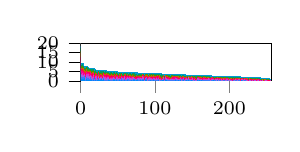
\begin{tikzpicture}

\definecolor{chocolate1961050}{RGB}{196,105,0}
\definecolor{crimson255078}{RGB}{255,0,78}
\definecolor{darkgray153}{RGB}{153,153,153}
\definecolor{darkslategray38}{RGB}{38,38,38}
\definecolor{darkslategray51}{RGB}{51,51,51}
\definecolor{darkturquoise0155207}{RGB}{0,155,207}
\definecolor{deeppink2510138}{RGB}{251,0,138}
\definecolor{dodgerblue0138250}{RGB}{0,138,250}
\definecolor{lightgray204}{RGB}{204,204,204}
\definecolor{mediumorchid21958191}{RGB}{219,58,191}
\definecolor{mediumpurple16495229}{RGB}{164,95,229}
\definecolor{olivedrab851440}{RGB}{85,144,0}
\definecolor{royalblue60122251}{RGB}{60,122,251}
\definecolor{teal015699}{RGB}{0,156,99}

\begin{axis}[
width=0.33\textwidth,
height=0.17\textwidth,
tick label style={font=\scriptsize},
tick align=outside,
tick pos=left,
xmin=0, xmax=256,
y grid style={darkgray176},
ymin=0, ymax=20,
ytick style={color=black},
ytick={0,5,10,15,20},
]
\addplot [semithick, darkgray153, forget plot]
table {%
0 4.44089209850063e-16
0 20
};
\draw[draw=none,fill=dodgerblue0138250] (axis cs:-0.35,0) rectangle (axis cs:0.35,4.15432851822353);

\draw[draw=none,fill=dodgerblue0138250] (axis cs:0.65,0) rectangle (axis cs:1.35,1.18287454765324);
\draw[draw=none,fill=dodgerblue0138250] (axis cs:1.65,0) rectangle (axis cs:2.35,0.93392293757018);
\draw[draw=none,fill=dodgerblue0138250] (axis cs:2.65,0) rectangle (axis cs:3.35,1.02254753069522);
\draw[draw=none,fill=dodgerblue0138250] (axis cs:3.65,0) rectangle (axis cs:4.35,1.76659823310965);
\draw[draw=none,fill=dodgerblue0138250] (axis cs:4.65,0) rectangle (axis cs:5.35,1.50319754690955);
\draw[draw=none,fill=dodgerblue0138250] (axis cs:5.65,0) rectangle (axis cs:6.35,0.344868445973939);
\draw[draw=none,fill=dodgerblue0138250] (axis cs:6.65,0) rectangle (axis cs:7.35,0.971287681877667);
\draw[draw=none,fill=dodgerblue0138250] (axis cs:7.65,0) rectangle (axis cs:8.35,0.91253338368545);
\draw[draw=none,fill=dodgerblue0138250] (axis cs:8.65,0) rectangle (axis cs:9.35,0.676711319617367);
\draw[draw=none,fill=dodgerblue0138250] (axis cs:9.65,0) rectangle (axis cs:10.35,1.50120257797594);
\draw[draw=none,fill=dodgerblue0138250] (axis cs:10.65,0) rectangle (axis cs:11.35,0.682743044726381);
\draw[draw=none,fill=dodgerblue0138250] (axis cs:11.65,0) rectangle (axis cs:12.35,0.739292129872664);
\draw[draw=none,fill=dodgerblue0138250] (axis cs:12.65,0) rectangle (axis cs:13.35,0.741122480440247);
\draw[draw=none,fill=dodgerblue0138250] (axis cs:13.65,0) rectangle (axis cs:14.35,0.986193417154741);
\draw[draw=none,fill=dodgerblue0138250] (axis cs:14.65,0) rectangle (axis cs:15.35,0.309545727759779);
\draw[draw=none,fill=dodgerblue0138250] (axis cs:15.65,0) rectangle (axis cs:16.35,0.539820774544653);
\draw[draw=none,fill=dodgerblue0138250] (axis cs:16.65,0) rectangle (axis cs:17.35,0.735583818268748);
\draw[draw=none,fill=dodgerblue0138250] (axis cs:17.65,0) rectangle (axis cs:18.35,0.494197409028206);
\draw[draw=none,fill=dodgerblue0138250] (axis cs:18.65,0) rectangle (axis cs:19.35,0.31060364920266);
\draw[draw=none,fill=dodgerblue0138250] (axis cs:19.65,0) rectangle (axis cs:20.35,0.484031876325862);
\draw[draw=none,fill=dodgerblue0138250] (axis cs:20.65,0) rectangle (axis cs:21.35,0.258779159330919);
\draw[draw=none,fill=dodgerblue0138250] (axis cs:21.65,0) rectangle (axis cs:22.35,0.341571106799856);
\draw[draw=none,fill=dodgerblue0138250] (axis cs:22.65,0) rectangle (axis cs:23.35,0.747810967597838);
\draw[draw=none,fill=dodgerblue0138250] (axis cs:23.65,0) rectangle (axis cs:24.35,0.822189644504438);
\draw[draw=none,fill=dodgerblue0138250] (axis cs:24.65,0) rectangle (axis cs:25.35,0.383568186929077);
\draw[draw=none,fill=dodgerblue0138250] (axis cs:25.65,0) rectangle (axis cs:26.35,0.710324499413359);
\draw[draw=none,fill=dodgerblue0138250] (axis cs:26.65,0) rectangle (axis cs:27.35,0.816734430228884);
\draw[draw=none,fill=dodgerblue0138250] (axis cs:27.65,0) rectangle (axis cs:28.35,1.12353593353567);
\draw[draw=none,fill=dodgerblue0138250] (axis cs:28.65,0) rectangle (axis cs:29.35,0.410578808280881);
\draw[draw=none,fill=dodgerblue0138250] (axis cs:29.65,0) rectangle (axis cs:30.35,0.966521379034545);
\draw[draw=none,fill=dodgerblue0138250] (axis cs:30.65,0) rectangle (axis cs:31.35,1.08995739350953);
\draw[draw=none,fill=dodgerblue0138250] (axis cs:31.65,0) rectangle (axis cs:32.35,0.344243565230843);
\draw[draw=none,fill=dodgerblue0138250] (axis cs:32.65,0) rectangle (axis cs:33.35,0.0951342426508125);
\draw[draw=none,fill=dodgerblue0138250] (axis cs:33.65,0) rectangle (axis cs:34.35,0.395473431714089);
\draw[draw=none,fill=dodgerblue0138250] (axis cs:34.65,0) rectangle (axis cs:35.35,0.42435291815903);
\draw[draw=none,fill=dodgerblue0138250] (axis cs:35.65,0) rectangle (axis cs:36.35,0.3015875956665);
\draw[draw=none,fill=dodgerblue0138250] (axis cs:36.65,0) rectangle (axis cs:37.35,0.388374629960168);
\draw[draw=none,fill=dodgerblue0138250] (axis cs:37.65,0) rectangle (axis cs:38.35,0.407769901876448);
\draw[draw=none,fill=dodgerblue0138250] (axis cs:38.65,0) rectangle (axis cs:39.35,0.480773769741225);
\draw[draw=none,fill=dodgerblue0138250] (axis cs:39.65,0) rectangle (axis cs:40.35,0.410709982911965);
\draw[draw=none,fill=dodgerblue0138250] (axis cs:40.65,0) rectangle (axis cs:41.35,0.366351380063404);
\draw[draw=none,fill=dodgerblue0138250] (axis cs:41.65,0) rectangle (axis cs:42.35,0.495468771783437);
\draw[draw=none,fill=dodgerblue0138250] (axis cs:42.65,0) rectangle (axis cs:43.35,0.299820416120711);
\draw[draw=none,fill=dodgerblue0138250] (axis cs:43.65,0) rectangle (axis cs:44.35,0.638683982264751);
\draw[draw=none,fill=dodgerblue0138250] (axis cs:44.65,0) rectangle (axis cs:45.35,0.461170180084615);
\draw[draw=none,fill=dodgerblue0138250] (axis cs:45.65,0) rectangle (axis cs:46.35,0.273886187992045);
\draw[draw=none,fill=dodgerblue0138250] (axis cs:46.65,0) rectangle (axis cs:47.35,0.451442077974514);
\draw[draw=none,fill=dodgerblue0138250] (axis cs:47.65,0) rectangle (axis cs:48.35,0.390202273163915);
\draw[draw=none,fill=dodgerblue0138250] (axis cs:48.65,0) rectangle (axis cs:49.35,0.174591931936953);
\draw[draw=none,fill=dodgerblue0138250] (axis cs:49.65,0) rectangle (axis cs:50.35,0.82017928366035);
\draw[draw=none,fill=dodgerblue0138250] (axis cs:50.65,0) rectangle (axis cs:51.35,0.397002144322494);
\draw[draw=none,fill=dodgerblue0138250] (axis cs:51.65,0) rectangle (axis cs:52.35,0.630474192775934);
\draw[draw=none,fill=dodgerblue0138250] (axis cs:52.65,0) rectangle (axis cs:53.35,0.508276784042551);
\draw[draw=none,fill=dodgerblue0138250] (axis cs:53.65,0) rectangle (axis cs:54.35,0.350520590466429);
\draw[draw=none,fill=dodgerblue0138250] (axis cs:54.65,0) rectangle (axis cs:55.35,0.529116710659704);
\draw[draw=none,fill=dodgerblue0138250] (axis cs:55.65,0) rectangle (axis cs:56.35,0.615406263230902);
\draw[draw=none,fill=dodgerblue0138250] (axis cs:56.65,0) rectangle (axis cs:57.35,0.226979778943014);
\draw[draw=none,fill=dodgerblue0138250] (axis cs:57.65,0) rectangle (axis cs:58.35,0.489624211234946);
\draw[draw=none,fill=dodgerblue0138250] (axis cs:58.65,0) rectangle (axis cs:59.35,0.458299962627676);
\draw[draw=none,fill=dodgerblue0138250] (axis cs:59.65,0) rectangle (axis cs:60.35,0.392567734528937);
\draw[draw=none,fill=dodgerblue0138250] (axis cs:60.65,0) rectangle (axis cs:61.35,0.185464126340538);
\draw[draw=none,fill=dodgerblue0138250] (axis cs:61.65,0) rectangle (axis cs:62.35,0.862219392272248);
\draw[draw=none,fill=dodgerblue0138250] (axis cs:62.65,0) rectangle (axis cs:63.35,0.34673351351619);
\draw[draw=none,fill=dodgerblue0138250] (axis cs:63.65,0) rectangle (axis cs:64.35,0.212593372078222);
\draw[draw=none,fill=dodgerblue0138250] (axis cs:64.65,0) rectangle (axis cs:65.35,0.521961567423149);
\draw[draw=none,fill=dodgerblue0138250] (axis cs:65.65,0) rectangle (axis cs:66.35,0.383562857462606);
\draw[draw=none,fill=dodgerblue0138250] (axis cs:66.65,0) rectangle (axis cs:67.35,0.452392890570174);
\draw[draw=none,fill=dodgerblue0138250] (axis cs:67.65,0) rectangle (axis cs:68.35,0.233243000800735);
\draw[draw=none,fill=dodgerblue0138250] (axis cs:68.65,0) rectangle (axis cs:69.35,0.251180969876626);
\draw[draw=none,fill=dodgerblue0138250] (axis cs:69.65,0) rectangle (axis cs:70.35,0.350768046407235);
\draw[draw=none,fill=dodgerblue0138250] (axis cs:70.65,0) rectangle (axis cs:71.35,0.556843614458057);
\draw[draw=none,fill=dodgerblue0138250] (axis cs:71.65,0) rectangle (axis cs:72.35,0.338413669351192);
\draw[draw=none,fill=dodgerblue0138250] (axis cs:72.65,0) rectangle (axis cs:73.35,0.311579608496369);
\draw[draw=none,fill=dodgerblue0138250] (axis cs:73.65,0) rectangle (axis cs:74.35,0.154240420336034);
\draw[draw=none,fill=dodgerblue0138250] (axis cs:74.65,0) rectangle (axis cs:75.35,0.437837362007211);
\draw[draw=none,fill=dodgerblue0138250] (axis cs:75.65,0) rectangle (axis cs:76.35,0.45627845662076);
\draw[draw=none,fill=dodgerblue0138250] (axis cs:76.65,0) rectangle (axis cs:77.35,0.168953653015007);
\draw[draw=none,fill=dodgerblue0138250] (axis cs:77.65,0) rectangle (axis cs:78.35,0.672928882322603);
\draw[draw=none,fill=dodgerblue0138250] (axis cs:78.65,0) rectangle (axis cs:79.35,0.54767338040339);
\draw[draw=none,fill=dodgerblue0138250] (axis cs:79.65,0) rectangle (axis cs:80.35,0.686353174522818);
\draw[draw=none,fill=dodgerblue0138250] (axis cs:80.65,0) rectangle (axis cs:81.35,0.150277625359469);
\draw[draw=none,fill=dodgerblue0138250] (axis cs:81.65,0) rectangle (axis cs:82.35,0.452457797949225);
\draw[draw=none,fill=dodgerblue0138250] (axis cs:82.65,0) rectangle (axis cs:83.35,0.41180795980092);
\draw[draw=none,fill=dodgerblue0138250] (axis cs:83.65,0) rectangle (axis cs:84.35,0.469436585730529);
\draw[draw=none,fill=dodgerblue0138250] (axis cs:84.65,0) rectangle (axis cs:85.35,0.16077608814991);
\draw[draw=none,fill=dodgerblue0138250] (axis cs:85.65,0) rectangle (axis cs:86.35,0.21460926447871);
\draw[draw=none,fill=dodgerblue0138250] (axis cs:86.65,0) rectangle (axis cs:87.35,0.290571129146703);
\draw[draw=none,fill=dodgerblue0138250] (axis cs:87.65,0) rectangle (axis cs:88.35,0.73505156764682);
\draw[draw=none,fill=dodgerblue0138250] (axis cs:88.65,0) rectangle (axis cs:89.35,0.187716947759467);
\draw[draw=none,fill=dodgerblue0138250] (axis cs:89.65,0) rectangle (axis cs:90.35,0.29454640450349);
\draw[draw=none,fill=dodgerblue0138250] (axis cs:90.65,0) rectangle (axis cs:91.35,0.499751319867372);
\draw[draw=none,fill=dodgerblue0138250] (axis cs:91.65,0) rectangle (axis cs:92.35,0.130998264536069);
\draw[draw=none,fill=dodgerblue0138250] (axis cs:92.65,0) rectangle (axis cs:93.35,0.405692321311318);
\draw[draw=none,fill=dodgerblue0138250] (axis cs:93.65,0) rectangle (axis cs:94.35,0.442530222820624);
\draw[draw=none,fill=dodgerblue0138250] (axis cs:94.65,0) rectangle (axis cs:95.35,0.390574583035228);
\draw[draw=none,fill=dodgerblue0138250] (axis cs:95.65,0) rectangle (axis cs:96.35,0.307422021573139);
\draw[draw=none,fill=dodgerblue0138250] (axis cs:96.65,0) rectangle (axis cs:97.35,0.14714340823868);
\draw[draw=none,fill=dodgerblue0138250] (axis cs:97.65,0) rectangle (axis cs:98.35,0.483308422713653);
\draw[draw=none,fill=dodgerblue0138250] (axis cs:98.65,0) rectangle (axis cs:99.35,0.394959304504547);
\draw[draw=none,fill=dodgerblue0138250] (axis cs:99.65,0) rectangle (axis cs:100.35,0.307620982908487);
\draw[draw=none,fill=dodgerblue0138250] (axis cs:100.65,0) rectangle (axis cs:101.35,0.430328365935788);
\draw[draw=none,fill=dodgerblue0138250] (axis cs:101.65,0) rectangle (axis cs:102.35,0.480806750195072);
\draw[draw=none,fill=dodgerblue0138250] (axis cs:102.65,0) rectangle (axis cs:103.35,0.226524463127423);
\draw[draw=none,fill=dodgerblue0138250] (axis cs:103.65,0) rectangle (axis cs:104.35,0.232669484847373);
\draw[draw=none,fill=dodgerblue0138250] (axis cs:104.65,0) rectangle (axis cs:105.35,0.339911118811259);
\draw[draw=none,fill=dodgerblue0138250] (axis cs:105.65,0) rectangle (axis cs:106.35,0.209235079057379);
\draw[draw=none,fill=dodgerblue0138250] (axis cs:106.65,0) rectangle (axis cs:107.35,0.235408126512755);
\draw[draw=none,fill=dodgerblue0138250] (axis cs:107.65,0) rectangle (axis cs:108.35,0.273991232352469);
\draw[draw=none,fill=dodgerblue0138250] (axis cs:108.65,0) rectangle (axis cs:109.35,0.155507196033846);
\draw[draw=none,fill=dodgerblue0138250] (axis cs:109.65,0) rectangle (axis cs:110.35,0.369195661231951);
\draw[draw=none,fill=dodgerblue0138250] (axis cs:110.65,0) rectangle (axis cs:111.35,0.536432794969108);
\draw[draw=none,fill=dodgerblue0138250] (axis cs:111.65,0) rectangle (axis cs:112.35,0.151347200352852);
\draw[draw=none,fill=dodgerblue0138250] (axis cs:112.65,0) rectangle (axis cs:113.35,0.345753776131098);
\draw[draw=none,fill=dodgerblue0138250] (axis cs:113.65,0) rectangle (axis cs:114.35,0.389869579187595);
\draw[draw=none,fill=dodgerblue0138250] (axis cs:114.65,0) rectangle (axis cs:115.35,0.226844478147403);
\draw[draw=none,fill=dodgerblue0138250] (axis cs:115.65,0) rectangle (axis cs:116.35,0.149996719644268);
\draw[draw=none,fill=dodgerblue0138250] (axis cs:116.65,0) rectangle (axis cs:117.35,0.752126199403964);
\draw[draw=none,fill=dodgerblue0138250] (axis cs:117.65,0) rectangle (axis cs:118.35,0.451285631261444);
\draw[draw=none,fill=dodgerblue0138250] (axis cs:118.65,0) rectangle (axis cs:119.35,0.30527884060474);
\draw[draw=none,fill=dodgerblue0138250] (axis cs:119.65,0) rectangle (axis cs:120.35,0.532174324161885);
\draw[draw=none,fill=dodgerblue0138250] (axis cs:120.65,0) rectangle (axis cs:121.35,0.573030859034782);
\draw[draw=none,fill=dodgerblue0138250] (axis cs:121.65,0) rectangle (axis cs:122.35,0.366156916316443);
\draw[draw=none,fill=dodgerblue0138250] (axis cs:122.65,0) rectangle (axis cs:123.35,0.137806647690384);
\draw[draw=none,fill=dodgerblue0138250] (axis cs:123.65,0) rectangle (axis cs:124.35,0.157079988088196);
\draw[draw=none,fill=dodgerblue0138250] (axis cs:124.65,0) rectangle (axis cs:125.35,0.559015438263524);
\draw[draw=none,fill=dodgerblue0138250] (axis cs:125.65,0) rectangle (axis cs:126.35,0.311421323467998);
\draw[draw=none,fill=dodgerblue0138250] (axis cs:126.65,0) rectangle (axis cs:127.35,0.644272400275388);
\draw[draw=none,fill=dodgerblue0138250] (axis cs:127.65,0) rectangle (axis cs:128.35,0.222071199581157);
\draw[draw=none,fill=dodgerblue0138250] (axis cs:128.65,0) rectangle (axis cs:129.35,0.511615849335944);
\draw[draw=none,fill=dodgerblue0138250] (axis cs:129.65,0) rectangle (axis cs:130.35,0.576325428627986);
\draw[draw=none,fill=dodgerblue0138250] (axis cs:130.65,0) rectangle (axis cs:131.35,0.38434299652847);
\draw[draw=none,fill=dodgerblue0138250] (axis cs:131.65,0) rectangle (axis cs:132.35,0.318669056721443);
\draw[draw=none,fill=dodgerblue0138250] (axis cs:132.65,0) rectangle (axis cs:133.35,0.226542573176072);
\draw[draw=none,fill=dodgerblue0138250] (axis cs:133.65,0) rectangle (axis cs:134.35,1.04193750808842);
\draw[draw=none,fill=dodgerblue0138250] (axis cs:134.65,0) rectangle (axis cs:135.35,0.269750155100022);
\draw[draw=none,fill=dodgerblue0138250] (axis cs:135.65,0) rectangle (axis cs:136.35,0.481729953826526);
\draw[draw=none,fill=dodgerblue0138250] (axis cs:136.65,0) rectangle (axis cs:137.35,0.217850830341202);
\draw[draw=none,fill=dodgerblue0138250] (axis cs:137.65,0) rectangle (axis cs:138.35,0.579921325632821);
\draw[draw=none,fill=dodgerblue0138250] (axis cs:138.65,0) rectangle (axis cs:139.35,0.185536111861042);
\draw[draw=none,fill=dodgerblue0138250] (axis cs:139.65,0) rectangle (axis cs:140.35,0.147446440426872);
\draw[draw=none,fill=dodgerblue0138250] (axis cs:140.65,0) rectangle (axis cs:141.35,0.419237045310767);
\draw[draw=none,fill=dodgerblue0138250] (axis cs:141.65,0) rectangle (axis cs:142.35,0.225695780427729);
\draw[draw=none,fill=dodgerblue0138250] (axis cs:142.65,0) rectangle (axis cs:143.35,0.349735747646733);
\draw[draw=none,fill=dodgerblue0138250] (axis cs:143.65,0) rectangle (axis cs:144.35,0.229668897154678);
\draw[draw=none,fill=dodgerblue0138250] (axis cs:144.65,0) rectangle (axis cs:145.35,0.741510378471586);
\draw[draw=none,fill=dodgerblue0138250] (axis cs:145.65,0) rectangle (axis cs:146.35,0.125753405472681);
\draw[draw=none,fill=dodgerblue0138250] (axis cs:146.65,0) rectangle (axis cs:147.35,0.288810810019723);
\draw[draw=none,fill=dodgerblue0138250] (axis cs:147.65,0) rectangle (axis cs:148.35,0.261705702233812);
\draw[draw=none,fill=dodgerblue0138250] (axis cs:148.65,0) rectangle (axis cs:149.35,0.334872921711527);
\draw[draw=none,fill=dodgerblue0138250] (axis cs:149.65,0) rectangle (axis cs:150.35,0.24815320349885);
\draw[draw=none,fill=dodgerblue0138250] (axis cs:150.65,0) rectangle (axis cs:151.35,0.23129983116906);
\draw[draw=none,fill=dodgerblue0138250] (axis cs:151.65,0) rectangle (axis cs:152.35,0.512755871999803);
\draw[draw=none,fill=dodgerblue0138250] (axis cs:152.65,0) rectangle (axis cs:153.35,0.41405988540184);
\draw[draw=none,fill=dodgerblue0138250] (axis cs:153.65,0) rectangle (axis cs:154.35,0.248914849694224);
\draw[draw=none,fill=dodgerblue0138250] (axis cs:154.65,0) rectangle (axis cs:155.35,0.301977078413934);
\draw[draw=none,fill=dodgerblue0138250] (axis cs:155.65,0) rectangle (axis cs:156.35,0.440251587998825);
\draw[draw=none,fill=dodgerblue0138250] (axis cs:156.65,0) rectangle (axis cs:157.35,0.356900408919444);
\draw[draw=none,fill=dodgerblue0138250] (axis cs:157.65,0) rectangle (axis cs:158.35,0.282423462764459);
\draw[draw=none,fill=dodgerblue0138250] (axis cs:158.65,0) rectangle (axis cs:159.35,0.465346758454599);
\draw[draw=none,fill=dodgerblue0138250] (axis cs:159.65,0) rectangle (axis cs:160.35,0.662633184375115);
\draw[draw=none,fill=dodgerblue0138250] (axis cs:160.65,0) rectangle (axis cs:161.35,0.514245706703937);
\draw[draw=none,fill=dodgerblue0138250] (axis cs:161.65,0) rectangle (axis cs:162.35,0.392379334946934);
\draw[draw=none,fill=dodgerblue0138250] (axis cs:162.65,0) rectangle (axis cs:163.35,0.380459535553755);
\draw[draw=none,fill=dodgerblue0138250] (axis cs:163.65,0) rectangle (axis cs:164.35,0.162909664488981);
\draw[draw=none,fill=dodgerblue0138250] (axis cs:164.65,0) rectangle (axis cs:165.35,0.441864261885323);
\draw[draw=none,fill=dodgerblue0138250] (axis cs:165.65,0) rectangle (axis cs:166.35,0.297948098586969);
\draw[draw=none,fill=dodgerblue0138250] (axis cs:166.65,0) rectangle (axis cs:167.35,0.408021026722375);
\draw[draw=none,fill=dodgerblue0138250] (axis cs:167.65,0) rectangle (axis cs:168.35,0.15691735477075);
\draw[draw=none,fill=dodgerblue0138250] (axis cs:168.65,0) rectangle (axis cs:169.35,0.238574401006548);
\draw[draw=none,fill=dodgerblue0138250] (axis cs:169.65,0) rectangle (axis cs:170.35,0.18288748348573);
\draw[draw=none,fill=dodgerblue0138250] (axis cs:170.65,0) rectangle (axis cs:171.35,0.134175407475566);
\draw[draw=none,fill=dodgerblue0138250] (axis cs:171.65,0) rectangle (axis cs:172.35,0.548664459947126);
\draw[draw=none,fill=dodgerblue0138250] (axis cs:172.65,0) rectangle (axis cs:173.35,0.337792952367299);
\draw[draw=none,fill=dodgerblue0138250] (axis cs:173.65,0) rectangle (axis cs:174.35,0.224078992003924);
\draw[draw=none,fill=dodgerblue0138250] (axis cs:174.65,0) rectangle (axis cs:175.35,0.561888043530945);
\draw[draw=none,fill=dodgerblue0138250] (axis cs:175.65,0) rectangle (axis cs:176.35,0.302691207295128);
\draw[draw=none,fill=dodgerblue0138250] (axis cs:176.65,0) rectangle (axis cs:177.35,0.118904378472481);
\draw[draw=none,fill=dodgerblue0138250] (axis cs:177.65,0) rectangle (axis cs:178.35,0.302649525671979);
\draw[draw=none,fill=dodgerblue0138250] (axis cs:178.65,0) rectangle (axis cs:179.35,0.342297679420432);
\draw[draw=none,fill=dodgerblue0138250] (axis cs:179.65,0) rectangle (axis cs:180.35,0.262720699925318);
\draw[draw=none,fill=dodgerblue0138250] (axis cs:180.65,0) rectangle (axis cs:181.35,0.215866565228983);
\draw[draw=none,fill=dodgerblue0138250] (axis cs:181.65,0) rectangle (axis cs:182.35,0.12100176879831);
\draw[draw=none,fill=dodgerblue0138250] (axis cs:182.65,0) rectangle (axis cs:183.35,0.312740060546427);
\draw[draw=none,fill=dodgerblue0138250] (axis cs:183.65,0) rectangle (axis cs:184.35,0.374256896540122);
\draw[draw=none,fill=dodgerblue0138250] (axis cs:184.65,0) rectangle (axis cs:185.35,0.218746772092042);
\draw[draw=none,fill=dodgerblue0138250] (axis cs:185.65,0) rectangle (axis cs:186.35,0.21700439097728);
\draw[draw=none,fill=dodgerblue0138250] (axis cs:186.65,0) rectangle (axis cs:187.35,0.422637594986668);
\draw[draw=none,fill=dodgerblue0138250] (axis cs:187.65,0) rectangle (axis cs:188.35,0.325650483252067);
\draw[draw=none,fill=dodgerblue0138250] (axis cs:188.65,0) rectangle (axis cs:189.35,0.114441431804835);
\draw[draw=none,fill=dodgerblue0138250] (axis cs:189.65,0) rectangle (axis cs:190.35,0.0670334444635619);
\draw[draw=none,fill=dodgerblue0138250] (axis cs:190.65,0) rectangle (axis cs:191.35,0.228441040055231);
\draw[draw=none,fill=dodgerblue0138250] (axis cs:191.65,0) rectangle (axis cs:192.35,0.484492083426825);
\draw[draw=none,fill=dodgerblue0138250] (axis cs:192.65,0) rectangle (axis cs:193.35,0.438898818837274);
\draw[draw=none,fill=dodgerblue0138250] (axis cs:193.65,0) rectangle (axis cs:194.35,0.123507106294804);
\draw[draw=none,fill=dodgerblue0138250] (axis cs:194.65,0) rectangle (axis cs:195.35,0.238777876149079);
\draw[draw=none,fill=dodgerblue0138250] (axis cs:195.65,0) rectangle (axis cs:196.35,0.197442820489827);
\draw[draw=none,fill=dodgerblue0138250] (axis cs:196.65,0) rectangle (axis cs:197.35,0.225236026086045);
\draw[draw=none,fill=dodgerblue0138250] (axis cs:197.65,0) rectangle (axis cs:198.35,0.294259236563487);
\draw[draw=none,fill=dodgerblue0138250] (axis cs:198.65,0) rectangle (axis cs:199.35,0.253278237548854);
\draw[draw=none,fill=dodgerblue0138250] (axis cs:199.65,0) rectangle (axis cs:200.35,0.137807306507893);
\draw[draw=none,fill=dodgerblue0138250] (axis cs:200.65,0) rectangle (axis cs:201.35,0.214895340038475);
\draw[draw=none,fill=dodgerblue0138250] (axis cs:201.65,0) rectangle (axis cs:202.35,0.231724660780255);
\draw[draw=none,fill=dodgerblue0138250] (axis cs:202.65,0) rectangle (axis cs:203.35,0.310228686671758);
\draw[draw=none,fill=dodgerblue0138250] (axis cs:203.65,0) rectangle (axis cs:204.35,0.173505186122126);
\draw[draw=none,fill=dodgerblue0138250] (axis cs:204.65,0) rectangle (axis cs:205.35,0.189631149989615);
\draw[draw=none,fill=dodgerblue0138250] (axis cs:205.65,0) rectangle (axis cs:206.35,0.34283395549007);
\draw[draw=none,fill=dodgerblue0138250] (axis cs:206.65,0) rectangle (axis cs:207.35,0.107028131106461);
\draw[draw=none,fill=dodgerblue0138250] (axis cs:207.65,0) rectangle (axis cs:208.35,0.100292583354001);
\draw[draw=none,fill=dodgerblue0138250] (axis cs:208.65,0) rectangle (axis cs:209.35,0.404300125348706);
\draw[draw=none,fill=dodgerblue0138250] (axis cs:209.65,0) rectangle (axis cs:210.35,0.274285596708935);
\draw[draw=none,fill=dodgerblue0138250] (axis cs:210.65,0) rectangle (axis cs:211.35,0.23853969832923);
\draw[draw=none,fill=dodgerblue0138250] (axis cs:211.65,0) rectangle (axis cs:212.35,0.177466240606106);
\draw[draw=none,fill=dodgerblue0138250] (axis cs:212.65,0) rectangle (axis cs:213.35,0.351179521082939);
\draw[draw=none,fill=dodgerblue0138250] (axis cs:213.65,0) rectangle (axis cs:214.35,0.236581529695006);
\draw[draw=none,fill=dodgerblue0138250] (axis cs:214.65,0) rectangle (axis cs:215.35,0.174846794935591);
\draw[draw=none,fill=dodgerblue0138250] (axis cs:215.65,0) rectangle (axis cs:216.35,0.261380526708587);
\draw[draw=none,fill=dodgerblue0138250] (axis cs:216.65,0) rectangle (axis cs:217.35,0.215763567338978);
\draw[draw=none,fill=dodgerblue0138250] (axis cs:217.65,0) rectangle (axis cs:218.35,0.24146476474904);
\draw[draw=none,fill=dodgerblue0138250] (axis cs:218.65,0) rectangle (axis cs:219.35,0.326698034376614);
\draw[draw=none,fill=dodgerblue0138250] (axis cs:219.65,0) rectangle (axis cs:220.35,0.191268540433577);
\draw[draw=none,fill=dodgerblue0138250] (axis cs:220.65,0) rectangle (axis cs:221.35,0.205206286865491);
\draw[draw=none,fill=dodgerblue0138250] (axis cs:221.65,0) rectangle (axis cs:222.35,0.2170673122199);
\draw[draw=none,fill=dodgerblue0138250] (axis cs:222.65,0) rectangle (axis cs:223.35,0.33074494651156);
\draw[draw=none,fill=dodgerblue0138250] (axis cs:223.65,0) rectangle (axis cs:224.35,0.181954520181725);
\draw[draw=none,fill=dodgerblue0138250] (axis cs:224.65,0) rectangle (axis cs:225.35,0.12426951387676);
\draw[draw=none,fill=dodgerblue0138250] (axis cs:225.65,0) rectangle (axis cs:226.35,0.307073406112646);
\draw[draw=none,fill=dodgerblue0138250] (axis cs:226.65,0) rectangle (axis cs:227.35,0.257772870751134);
\draw[draw=none,fill=dodgerblue0138250] (axis cs:227.65,0) rectangle (axis cs:228.35,0.195434548863174);
\draw[draw=none,fill=dodgerblue0138250] (axis cs:228.65,0) rectangle (axis cs:229.35,0.122985925790121);
\draw[draw=none,fill=dodgerblue0138250] (axis cs:229.65,0) rectangle (axis cs:230.35,0.101226797718072);
\draw[draw=none,fill=dodgerblue0138250] (axis cs:230.65,0) rectangle (axis cs:231.35,0.178475276189003);
\draw[draw=none,fill=dodgerblue0138250] (axis cs:231.65,0) rectangle (axis cs:232.35,0.105363515726292);
\draw[draw=none,fill=dodgerblue0138250] (axis cs:232.65,0) rectangle (axis cs:233.35,0.0762180944171262);
\draw[draw=none,fill=dodgerblue0138250] (axis cs:233.65,0) rectangle (axis cs:234.35,0.235939455372723);
\draw[draw=none,fill=dodgerblue0138250] (axis cs:234.65,0) rectangle (axis cs:235.35,0.195412711386573);
\draw[draw=none,fill=dodgerblue0138250] (axis cs:235.65,0) rectangle (axis cs:236.35,0.131155366177);
\draw[draw=none,fill=dodgerblue0138250] (axis cs:236.65,0) rectangle (axis cs:237.35,0.297734924062318);
\draw[draw=none,fill=dodgerblue0138250] (axis cs:237.65,0) rectangle (axis cs:238.35,0.146779686740578);
\draw[draw=none,fill=dodgerblue0138250] (axis cs:238.65,0) rectangle (axis cs:239.35,0.310163106613969);
\draw[draw=none,fill=dodgerblue0138250] (axis cs:239.65,0) rectangle (axis cs:240.35,0.117985726594922);
\draw[draw=none,fill=dodgerblue0138250] (axis cs:240.65,0) rectangle (axis cs:241.35,0.0847952112397484);
\draw[draw=none,fill=dodgerblue0138250] (axis cs:241.65,0) rectangle (axis cs:242.35,0.141669876554581);
\draw[draw=none,fill=dodgerblue0138250] (axis cs:242.65,0) rectangle (axis cs:243.35,0.105256102268126);
\draw[draw=none,fill=dodgerblue0138250] (axis cs:243.65,0) rectangle (axis cs:244.35,0.174722555708435);
\draw[draw=none,fill=dodgerblue0138250] (axis cs:244.65,0) rectangle (axis cs:245.35,0.274283397457468);
\draw[draw=none,fill=dodgerblue0138250] (axis cs:245.65,0) rectangle (axis cs:246.35,0.0929868411034279);
\draw[draw=none,fill=dodgerblue0138250] (axis cs:246.65,0) rectangle (axis cs:247.35,0.159236693550173);
\draw[draw=none,fill=dodgerblue0138250] (axis cs:247.65,0) rectangle (axis cs:248.35,0.159577752176232);
\draw[draw=none,fill=dodgerblue0138250] (axis cs:248.65,0) rectangle (axis cs:249.35,0.289232100827197);
\draw[draw=none,fill=dodgerblue0138250] (axis cs:249.65,0) rectangle (axis cs:250.35,0.19687232270575);
\draw[draw=none,fill=dodgerblue0138250] (axis cs:250.65,0) rectangle (axis cs:251.35,0.129840628792184);
\draw[draw=none,fill=dodgerblue0138250] (axis cs:251.65,0) rectangle (axis cs:252.35,0.0863024713699495);
\draw[draw=none,fill=dodgerblue0138250] (axis cs:252.65,0) rectangle (axis cs:253.35,0.0985359522280668);
\draw[draw=none,fill=dodgerblue0138250] (axis cs:253.65,0) rectangle (axis cs:254.35,0.135306124249902);
\draw[draw=none,fill=dodgerblue0138250] (axis cs:254.65,0) rectangle (axis cs:255.35,0.204258697442185);
\draw[draw=none,fill=royalblue60122251] (axis cs:-0.35,4.15432851822353) rectangle (axis cs:0.35,4.74723706865037);

\draw[draw=none,fill=royalblue60122251] (axis cs:0.65,1.18287454765324) rectangle (axis cs:1.35,2.00123347871187);
\draw[draw=none,fill=royalblue60122251] (axis cs:1.65,0.93392293757018) rectangle (axis cs:2.35,1.97936894757984);
\draw[draw=none,fill=royalblue60122251] (axis cs:2.65,1.02254753069522) rectangle (axis cs:3.35,2.35465379609693);
\draw[draw=none,fill=royalblue60122251] (axis cs:3.65,1.76659823310965) rectangle (axis cs:4.35,2.02890096160253);
\draw[draw=none,fill=royalblue60122251] (axis cs:4.65,1.50319754690955) rectangle (axis cs:5.35,2.72251969544056);
\draw[draw=none,fill=royalblue60122251] (axis cs:5.65,0.344868445973939) rectangle (axis cs:6.35,0.702095654837144);
\draw[draw=none,fill=royalblue60122251] (axis cs:6.65,0.971287681877667) rectangle (axis cs:7.35,1.32647166974035);
\draw[draw=none,fill=royalblue60122251] (axis cs:7.65,0.91253338368545) rectangle (axis cs:8.35,2.06630352125954);
\draw[draw=none,fill=royalblue60122251] (axis cs:8.65,0.676711319617367) rectangle (axis cs:9.35,1.34167309636743);
\draw[draw=none,fill=royalblue60122251] (axis cs:9.65,1.50120257797594) rectangle (axis cs:10.35,2.46583009095569);
\draw[draw=none,fill=royalblue60122251] (axis cs:10.65,0.682743044726381) rectangle (axis cs:11.35,1.42176969366789);
\draw[draw=none,fill=royalblue60122251] (axis cs:11.65,0.739292129872664) rectangle (axis cs:12.35,1.12326283577694);
\draw[draw=none,fill=royalblue60122251] (axis cs:12.65,0.741122480440247) rectangle (axis cs:13.35,1.91840872936836);
\draw[draw=none,fill=royalblue60122251] (axis cs:13.65,0.986193417154741) rectangle (axis cs:14.35,2.33053108046494);
\draw[draw=none,fill=royalblue60122251] (axis cs:14.65,0.309545727759779) rectangle (axis cs:15.35,0.951660252428782);
\draw[draw=none,fill=royalblue60122251] (axis cs:15.65,0.539820774544653) rectangle (axis cs:16.35,0.693824474021026);
\draw[draw=none,fill=royalblue60122251] (axis cs:16.65,0.735583818268748) rectangle (axis cs:17.35,1.45602869279533);
\draw[draw=none,fill=royalblue60122251] (axis cs:17.65,0.494197409028206) rectangle (axis cs:18.35,0.973270006410257);
\draw[draw=none,fill=royalblue60122251] (axis cs:18.65,0.31060364920266) rectangle (axis cs:19.35,0.644900937063916);
\draw[draw=none,fill=royalblue60122251] (axis cs:19.65,0.484031876325862) rectangle (axis cs:20.35,1.74768257614376);
\draw[draw=none,fill=royalblue60122251] (axis cs:20.65,0.258779159330919) rectangle (axis cs:21.35,0.723585224717224);
\draw[draw=none,fill=royalblue60122251] (axis cs:21.65,0.341571106799856) rectangle (axis cs:22.35,0.904642747471537);
\draw[draw=none,fill=royalblue60122251] (axis cs:22.65,0.747810967597838) rectangle (axis cs:23.35,1.11854524068239);
\draw[draw=none,fill=royalblue60122251] (axis cs:23.65,0.822189644504438) rectangle (axis cs:24.35,1.68040803788798);
\draw[draw=none,fill=royalblue60122251] (axis cs:24.65,0.383568186929077) rectangle (axis cs:25.35,0.880521601318662);
\draw[draw=none,fill=royalblue60122251] (axis cs:25.65,0.710324499413359) rectangle (axis cs:26.35,1.02303358588476);
\draw[draw=none,fill=royalblue60122251] (axis cs:26.65,0.816734430228884) rectangle (axis cs:27.35,1.78032483252688);
\draw[draw=none,fill=royalblue60122251] (axis cs:27.65,1.12353593353567) rectangle (axis cs:28.35,1.46790755061758);
\draw[draw=none,fill=royalblue60122251] (axis cs:28.65,0.410578808280881) rectangle (axis cs:29.35,0.978970304366244);
\draw[draw=none,fill=royalblue60122251] (axis cs:29.65,0.966521379034545) rectangle (axis cs:30.35,1.39976040274279);
\draw[draw=none,fill=royalblue60122251] (axis cs:30.65,1.08995739350953) rectangle (axis cs:31.35,1.67797559231924);
\draw[draw=none,fill=royalblue60122251] (axis cs:31.65,0.344243565230843) rectangle (axis cs:32.35,0.71205431731836);
\draw[draw=none,fill=royalblue60122251] (axis cs:32.65,0.0951342426508125) rectangle (axis cs:33.35,0.239544138250011);
\draw[draw=none,fill=royalblue60122251] (axis cs:33.65,0.395473431714089) rectangle (axis cs:34.35,0.666579988983834);
\draw[draw=none,fill=royalblue60122251] (axis cs:34.65,0.42435291815903) rectangle (axis cs:35.35,2.02004478739436);
\draw[draw=none,fill=royalblue60122251] (axis cs:35.65,0.3015875956665) rectangle (axis cs:36.35,0.608787846058352);
\draw[draw=none,fill=royalblue60122251] (axis cs:36.65,0.388374629960168) rectangle (axis cs:37.35,1.03250379628287);
\draw[draw=none,fill=royalblue60122251] (axis cs:37.65,0.407769901876448) rectangle (axis cs:38.35,0.943289320472076);
\draw[draw=none,fill=royalblue60122251] (axis cs:38.65,0.480773769741225) rectangle (axis cs:39.35,0.804665108246466);
\draw[draw=none,fill=royalblue60122251] (axis cs:39.65,0.410709982911965) rectangle (axis cs:40.35,0.668276625289806);
\draw[draw=none,fill=royalblue60122251] (axis cs:40.65,0.366351380063404) rectangle (axis cs:41.35,0.673871980259898);
\draw[draw=none,fill=royalblue60122251] (axis cs:41.65,0.495468771783437) rectangle (axis cs:42.35,0.749202415690694);
\draw[draw=none,fill=royalblue60122251] (axis cs:42.65,0.299820416120711) rectangle (axis cs:43.35,0.738197935120244);
\draw[draw=none,fill=royalblue60122251] (axis cs:43.65,0.638683982264751) rectangle (axis cs:44.35,0.872951604519205);
\draw[draw=none,fill=royalblue60122251] (axis cs:44.65,0.461170180084615) rectangle (axis cs:45.35,1.10466197054807);
\draw[draw=none,fill=royalblue60122251] (axis cs:45.65,0.273886187992045) rectangle (axis cs:46.35,0.675631832252773);
\draw[draw=none,fill=royalblue60122251] (axis cs:46.65,0.451442077974514) rectangle (axis cs:47.35,1.30937687658285);
\draw[draw=none,fill=royalblue60122251] (axis cs:47.65,0.390202273163915) rectangle (axis cs:48.35,1.13223984110611);
\draw[draw=none,fill=royalblue60122251] (axis cs:48.65,0.174591931936953) rectangle (axis cs:49.35,0.781112586155575);
\draw[draw=none,fill=royalblue60122251] (axis cs:49.65,0.82017928366035) rectangle (axis cs:50.35,1.07487395162565);
\draw[draw=none,fill=royalblue60122251] (axis cs:50.65,0.397002144322494) rectangle (axis cs:51.35,0.521571913071357);
\draw[draw=none,fill=royalblue60122251] (axis cs:51.65,0.630474192775934) rectangle (axis cs:52.35,1.10493075596636);
\draw[draw=none,fill=royalblue60122251] (axis cs:52.65,0.508276784042551) rectangle (axis cs:53.35,1.45392728991268);
\draw[draw=none,fill=royalblue60122251] (axis cs:53.65,0.350520590466429) rectangle (axis cs:54.35,0.709538571188494);
\draw[draw=none,fill=royalblue60122251] (axis cs:54.65,0.529116710659704) rectangle (axis cs:55.35,1.56916645184503);
\draw[draw=none,fill=royalblue60122251] (axis cs:55.65,0.615406263230902) rectangle (axis cs:56.35,0.725115105753118);
\draw[draw=none,fill=royalblue60122251] (axis cs:56.65,0.226979778943014) rectangle (axis cs:57.35,0.984918273826488);
\draw[draw=none,fill=royalblue60122251] (axis cs:57.65,0.489624211234946) rectangle (axis cs:58.35,0.626692030825994);
\draw[draw=none,fill=royalblue60122251] (axis cs:58.65,0.458299962627676) rectangle (axis cs:59.35,0.957708470199095);
\draw[draw=none,fill=royalblue60122251] (axis cs:59.65,0.392567734528937) rectangle (axis cs:60.35,0.519887299919797);
\draw[draw=none,fill=royalblue60122251] (axis cs:60.65,0.185464126340538) rectangle (axis cs:61.35,0.416192151876631);
\draw[draw=none,fill=royalblue60122251] (axis cs:61.65,0.862219392272248) rectangle (axis cs:62.35,1.59371614289329);
\draw[draw=none,fill=royalblue60122251] (axis cs:62.65,0.34673351351619) rectangle (axis cs:63.35,1.22629308709323);
\draw[draw=none,fill=royalblue60122251] (axis cs:63.65,0.212593372078222) rectangle (axis cs:64.35,0.866200292972699);
\draw[draw=none,fill=royalblue60122251] (axis cs:64.65,0.521961567423149) rectangle (axis cs:65.35,0.712680950241972);
\draw[draw=none,fill=royalblue60122251] (axis cs:65.65,0.383562857462606) rectangle (axis cs:66.35,0.947555554363721);
\draw[draw=none,fill=royalblue60122251] (axis cs:66.65,0.452392890570174) rectangle (axis cs:67.35,0.742586629837577);
\draw[draw=none,fill=royalblue60122251] (axis cs:67.65,0.233243000800735) rectangle (axis cs:68.35,0.963899890130031);
\draw[draw=none,fill=royalblue60122251] (axis cs:68.65,0.251180969876626) rectangle (axis cs:69.35,0.432843188860383);
\draw[draw=none,fill=royalblue60122251] (axis cs:69.65,0.350768046407235) rectangle (axis cs:70.35,0.591792062164883);
\draw[draw=none,fill=royalblue60122251] (axis cs:70.65,0.556843614458057) rectangle (axis cs:71.35,1.20321109515648);
\draw[draw=none,fill=royalblue60122251] (axis cs:71.65,0.338413669351192) rectangle (axis cs:72.35,1.1865607021829);
\draw[draw=none,fill=royalblue60122251] (axis cs:72.65,0.311579608496369) rectangle (axis cs:73.35,1.08281991951923);
\draw[draw=none,fill=royalblue60122251] (axis cs:73.65,0.154240420336034) rectangle (axis cs:74.35,0.496419312193075);
\draw[draw=none,fill=royalblue60122251] (axis cs:74.65,0.437837362007211) rectangle (axis cs:75.35,0.846890954980125);
\draw[draw=none,fill=royalblue60122251] (axis cs:75.65,0.45627845662076) rectangle (axis cs:76.35,0.835065595982998);
\draw[draw=none,fill=royalblue60122251] (axis cs:76.65,0.168953653015007) rectangle (axis cs:77.35,0.683642547848915);
\draw[draw=none,fill=royalblue60122251] (axis cs:77.65,0.672928882322603) rectangle (axis cs:78.35,0.837788858270383);
\draw[draw=none,fill=royalblue60122251] (axis cs:78.65,0.54767338040339) rectangle (axis cs:79.35,0.717840161655212);
\draw[draw=none,fill=royalblue60122251] (axis cs:79.65,0.686353174522818) rectangle (axis cs:80.35,1.33961453963284);
\draw[draw=none,fill=royalblue60122251] (axis cs:80.65,0.150277625359469) rectangle (axis cs:81.35,0.883118149898528);
\draw[draw=none,fill=royalblue60122251] (axis cs:81.65,0.452457797949225) rectangle (axis cs:82.35,0.712742123664412);
\draw[draw=none,fill=royalblue60122251] (axis cs:82.65,0.41180795980092) rectangle (axis cs:83.35,1.16368888146753);
\draw[draw=none,fill=royalblue60122251] (axis cs:83.65,0.469436585730529) rectangle (axis cs:84.35,1.54457035146808);
\draw[draw=none,fill=royalblue60122251] (axis cs:84.65,0.16077608814991) rectangle (axis cs:85.35,0.387769872331446);
\draw[draw=none,fill=royalblue60122251] (axis cs:85.65,0.21460926447871) rectangle (axis cs:86.35,0.298578913666278);
\draw[draw=none,fill=royalblue60122251] (axis cs:86.65,0.290571129146703) rectangle (axis cs:87.35,1.49637751678828);
\draw[draw=none,fill=royalblue60122251] (axis cs:87.65,0.73505156764682) rectangle (axis cs:88.35,1.61533065420132);
\draw[draw=none,fill=royalblue60122251] (axis cs:88.65,0.187716947759467) rectangle (axis cs:89.35,0.396431291875083);
\draw[draw=none,fill=royalblue60122251] (axis cs:89.65,0.29454640450349) rectangle (axis cs:90.35,1.25575746812791);
\draw[draw=none,fill=royalblue60122251] (axis cs:90.65,0.499751319867372) rectangle (axis cs:91.35,0.699048982745992);
\draw[draw=none,fill=royalblue60122251] (axis cs:91.65,0.130998264536069) rectangle (axis cs:92.35,0.544462411941945);
\draw[draw=none,fill=royalblue60122251] (axis cs:92.65,0.405692321311318) rectangle (axis cs:93.35,1.01350580267539);
\draw[draw=none,fill=royalblue60122251] (axis cs:93.65,0.442530222820624) rectangle (axis cs:94.35,0.755170690452478);
\draw[draw=none,fill=royalblue60122251] (axis cs:94.65,0.390574583035228) rectangle (axis cs:95.35,0.618445799136912);
\draw[draw=none,fill=royalblue60122251] (axis cs:95.65,0.307422021573139) rectangle (axis cs:96.35,1.11035392216481);
\draw[draw=none,fill=royalblue60122251] (axis cs:96.65,0.14714340823868) rectangle (axis cs:97.35,0.699576622754806);
\draw[draw=none,fill=royalblue60122251] (axis cs:97.65,0.483308422713653) rectangle (axis cs:98.35,0.760392937695533);
\draw[draw=none,fill=royalblue60122251] (axis cs:98.65,0.394959304504547) rectangle (axis cs:99.35,0.675657889037019);
\draw[draw=none,fill=royalblue60122251] (axis cs:99.65,0.307620982908487) rectangle (axis cs:100.35,0.50066229012851);
\draw[draw=none,fill=royalblue60122251] (axis cs:100.65,0.430328365935788) rectangle (axis cs:101.35,0.743214843711653);
\draw[draw=none,fill=royalblue60122251] (axis cs:101.65,0.480806750195072) rectangle (axis cs:102.35,0.70285208310079);
\draw[draw=none,fill=royalblue60122251] (axis cs:102.65,0.226524463127423) rectangle (axis cs:103.35,0.352220561632304);
\draw[draw=none,fill=royalblue60122251] (axis cs:103.65,0.232669484847373) rectangle (axis cs:104.35,1.20381396846466);
\draw[draw=none,fill=royalblue60122251] (axis cs:104.65,0.339911118811259) rectangle (axis cs:105.35,1.07576942148295);
\draw[draw=none,fill=royalblue60122251] (axis cs:105.65,0.209235079057379) rectangle (axis cs:106.35,0.47278641392541);
\draw[draw=none,fill=royalblue60122251] (axis cs:106.65,0.235408126512755) rectangle (axis cs:107.35,0.66307502489773);
\draw[draw=none,fill=royalblue60122251] (axis cs:107.65,0.273991232352469) rectangle (axis cs:108.35,0.572638976048701);
\draw[draw=none,fill=royalblue60122251] (axis cs:108.65,0.155507196033846) rectangle (axis cs:109.35,0.551049087143373);
\draw[draw=none,fill=royalblue60122251] (axis cs:109.65,0.369195661231951) rectangle (axis cs:110.35,0.752698451463311);
\draw[draw=none,fill=royalblue60122251] (axis cs:110.65,0.536432794969108) rectangle (axis cs:111.35,0.982098615078709);
\draw[draw=none,fill=royalblue60122251] (axis cs:111.65,0.151347200352852) rectangle (axis cs:112.35,0.442471954529165);
\draw[draw=none,fill=royalblue60122251] (axis cs:112.65,0.345753776131098) rectangle (axis cs:113.35,0.644310521962149);
\draw[draw=none,fill=royalblue60122251] (axis cs:113.65,0.389869579187595) rectangle (axis cs:114.35,0.934605233670275);
\draw[draw=none,fill=royalblue60122251] (axis cs:114.65,0.226844478147403) rectangle (axis cs:115.35,0.996090075670197);
\draw[draw=none,fill=royalblue60122251] (axis cs:115.65,0.149996719644268) rectangle (axis cs:116.35,0.328890839550644);
\draw[draw=none,fill=royalblue60122251] (axis cs:116.65,0.752126199403964) rectangle (axis cs:117.35,1.25954629819177);
\draw[draw=none,fill=royalblue60122251] (axis cs:117.65,0.451285631261444) rectangle (axis cs:118.35,0.675221054874825);
\draw[draw=none,fill=royalblue60122251] (axis cs:118.65,0.30527884060474) rectangle (axis cs:119.35,0.602589986433383);
\draw[draw=none,fill=royalblue60122251] (axis cs:119.65,0.532174324161885) rectangle (axis cs:120.35,0.665262478730331);
\draw[draw=none,fill=royalblue60122251] (axis cs:120.65,0.573030859034782) rectangle (axis cs:121.35,0.818789610292948);
\draw[draw=none,fill=royalblue60122251] (axis cs:121.65,0.366156916316443) rectangle (axis cs:122.35,0.519750863161122);
\draw[draw=none,fill=royalblue60122251] (axis cs:122.65,0.137806647690384) rectangle (axis cs:123.35,0.521250208319364);
\draw[draw=none,fill=royalblue60122251] (axis cs:123.65,0.157079988088196) rectangle (axis cs:124.35,0.343004118559861);
\draw[draw=none,fill=royalblue60122251] (axis cs:124.65,0.559015438263524) rectangle (axis cs:125.35,0.865111669102709);
\draw[draw=none,fill=royalblue60122251] (axis cs:125.65,0.311421323467998) rectangle (axis cs:126.35,0.453952522376491);
\draw[draw=none,fill=royalblue60122251] (axis cs:126.65,0.644272400275388) rectangle (axis cs:127.35,1.09079580040487);
\draw[draw=none,fill=royalblue60122251] (axis cs:127.65,0.222071199581157) rectangle (axis cs:128.35,0.604669742138209);
\draw[draw=none,fill=royalblue60122251] (axis cs:128.65,0.511615849335944) rectangle (axis cs:129.35,0.899324993871569);
\draw[draw=none,fill=royalblue60122251] (axis cs:129.65,0.576325428627986) rectangle (axis cs:130.35,0.739665093540699);
\draw[draw=none,fill=royalblue60122251] (axis cs:130.65,0.38434299652847) rectangle (axis cs:131.35,1.01590260975965);
\draw[draw=none,fill=royalblue60122251] (axis cs:131.65,0.318669056721443) rectangle (axis cs:132.35,1.08415150312914);
\draw[draw=none,fill=royalblue60122251] (axis cs:132.65,0.226542573176072) rectangle (axis cs:133.35,0.714018930035271);
\draw[draw=none,fill=royalblue60122251] (axis cs:133.65,1.04193750808842) rectangle (axis cs:134.35,1.24813136215339);
\draw[draw=none,fill=royalblue60122251] (axis cs:134.65,0.269750155100022) rectangle (axis cs:135.35,0.41351534161047);
\draw[draw=none,fill=royalblue60122251] (axis cs:135.65,0.481729953826526) rectangle (axis cs:136.35,0.819335542033602);
\draw[draw=none,fill=royalblue60122251] (axis cs:136.65,0.217850830341202) rectangle (axis cs:137.35,0.90788496468897);
\draw[draw=none,fill=royalblue60122251] (axis cs:137.65,0.579921325632821) rectangle (axis cs:138.35,0.792726553362071);
\draw[draw=none,fill=royalblue60122251] (axis cs:138.65,0.185536111861042) rectangle (axis cs:139.35,0.273880917979959);
\draw[draw=none,fill=royalblue60122251] (axis cs:139.65,0.147446440426872) rectangle (axis cs:140.35,0.84516788420012);
\draw[draw=none,fill=royalblue60122251] (axis cs:140.65,0.419237045310767) rectangle (axis cs:141.35,0.564804475912843);
\draw[draw=none,fill=royalblue60122251] (axis cs:141.65,0.225695780427729) rectangle (axis cs:142.35,0.958806981813776);
\draw[draw=none,fill=royalblue60122251] (axis cs:142.65,0.349735747646733) rectangle (axis cs:143.35,1.00970248499124);
\draw[draw=none,fill=royalblue60122251] (axis cs:143.65,0.229668897154678) rectangle (axis cs:144.35,0.464594591530454);
\draw[draw=none,fill=royalblue60122251] (axis cs:144.65,0.741510378471586) rectangle (axis cs:145.35,1.21013301793736);
\draw[draw=none,fill=royalblue60122251] (axis cs:145.65,0.125753405472681) rectangle (axis cs:146.35,0.263188851689383);
\draw[draw=none,fill=royalblue60122251] (axis cs:146.65,0.288810810019723) rectangle (axis cs:147.35,0.378051855936352);
\draw[draw=none,fill=royalblue60122251] (axis cs:147.65,0.261705702233812) rectangle (axis cs:148.35,0.788162472670737);
\draw[draw=none,fill=royalblue60122251] (axis cs:148.65,0.334872921711527) rectangle (axis cs:149.35,0.781360712698226);
\draw[draw=none,fill=royalblue60122251] (axis cs:149.65,0.24815320349885) rectangle (axis cs:150.35,0.679288793966836);
\draw[draw=none,fill=royalblue60122251] (axis cs:150.65,0.23129983116906) rectangle (axis cs:151.35,0.331005348676946);
\draw[draw=none,fill=royalblue60122251] (axis cs:151.65,0.512755871999803) rectangle (axis cs:152.35,0.912476243818507);
\draw[draw=none,fill=royalblue60122251] (axis cs:152.65,0.41405988540184) rectangle (axis cs:153.35,0.656043271819433);
\draw[draw=none,fill=royalblue60122251] (axis cs:153.65,0.248914849694224) rectangle (axis cs:154.35,0.553693728636288);
\draw[draw=none,fill=royalblue60122251] (axis cs:154.65,0.301977078413934) rectangle (axis cs:155.35,0.417078589291807);
\draw[draw=none,fill=royalblue60122251] (axis cs:155.65,0.440251587998825) rectangle (axis cs:156.35,0.745071783109115);
\draw[draw=none,fill=royalblue60122251] (axis cs:156.65,0.356900408919444) rectangle (axis cs:157.35,0.936645042248307);
\draw[draw=none,fill=royalblue60122251] (axis cs:157.65,0.282423462764459) rectangle (axis cs:158.35,0.435470512599823);
\draw[draw=none,fill=royalblue60122251] (axis cs:158.65,0.465346758454599) rectangle (axis cs:159.35,0.874146067529543);
\draw[draw=none,fill=royalblue60122251] (axis cs:159.65,0.662633184375115) rectangle (axis cs:160.35,0.769391488700568);
\draw[draw=none,fill=royalblue60122251] (axis cs:160.65,0.514245706703937) rectangle (axis cs:161.35,0.591997636843377);
\draw[draw=none,fill=royalblue60122251] (axis cs:161.65,0.392379334946934) rectangle (axis cs:162.35,0.853351253093966);
\draw[draw=none,fill=royalblue60122251] (axis cs:162.65,0.380459535553755) rectangle (axis cs:163.35,0.739485987619591);
\draw[draw=none,fill=royalblue60122251] (axis cs:163.65,0.162909664488981) rectangle (axis cs:164.35,0.686698079067279);
\draw[draw=none,fill=royalblue60122251] (axis cs:164.65,0.441864261885323) rectangle (axis cs:165.35,0.519055676962012);
\draw[draw=none,fill=royalblue60122251] (axis cs:165.65,0.297948098586969) rectangle (axis cs:166.35,0.558072935080633);
\draw[draw=none,fill=royalblue60122251] (axis cs:166.65,0.408021026722375) rectangle (axis cs:167.35,0.879303403570161);
\draw[draw=none,fill=royalblue60122251] (axis cs:167.65,0.15691735477075) rectangle (axis cs:168.35,0.520957964529232);
\draw[draw=none,fill=royalblue60122251] (axis cs:168.65,0.238574401006548) rectangle (axis cs:169.35,0.505369354351369);
\draw[draw=none,fill=royalblue60122251] (axis cs:169.65,0.18288748348573) rectangle (axis cs:170.35,0.749075035701437);
\draw[draw=none,fill=royalblue60122251] (axis cs:170.65,0.134175407475566) rectangle (axis cs:171.35,0.70024733525597);
\draw[draw=none,fill=royalblue60122251] (axis cs:171.65,0.548664459947126) rectangle (axis cs:172.35,1.03730030556115);
\draw[draw=none,fill=royalblue60122251] (axis cs:172.65,0.337792952367299) rectangle (axis cs:173.35,0.721647743148849);
\draw[draw=none,fill=royalblue60122251] (axis cs:173.65,0.224078992003924) rectangle (axis cs:174.35,0.330670655406056);
\draw[draw=none,fill=royalblue60122251] (axis cs:174.65,0.561888043530945) rectangle (axis cs:175.35,0.672955459106589);
\draw[draw=none,fill=royalblue60122251] (axis cs:175.65,0.302691207295128) rectangle (axis cs:176.35,0.78561548273326);
\draw[draw=none,fill=royalblue60122251] (axis cs:176.65,0.118904378472481) rectangle (axis cs:177.35,0.520523037552239);
\draw[draw=none,fill=royalblue60122251] (axis cs:177.65,0.302649525671979) rectangle (axis cs:178.35,0.889941693477215);
\draw[draw=none,fill=royalblue60122251] (axis cs:178.65,0.342297679420432) rectangle (axis cs:179.35,0.452756152582567);
\draw[draw=none,fill=royalblue60122251] (axis cs:179.65,0.262720699925318) rectangle (axis cs:180.35,0.805262668662307);
\draw[draw=none,fill=royalblue60122251] (axis cs:180.65,0.215866565228983) rectangle (axis cs:181.35,0.493200893724844);
\draw[draw=none,fill=royalblue60122251] (axis cs:181.65,0.12100176879831) rectangle (axis cs:182.35,0.253165208998005);
\draw[draw=none,fill=royalblue60122251] (axis cs:182.65,0.312740060546427) rectangle (axis cs:183.35,0.769418914930401);
\draw[draw=none,fill=royalblue60122251] (axis cs:183.65,0.374256896540122) rectangle (axis cs:184.35,0.787340048206036);
\draw[draw=none,fill=royalblue60122251] (axis cs:184.65,0.218746772092042) rectangle (axis cs:185.35,0.307249165265595);
\draw[draw=none,fill=royalblue60122251] (axis cs:185.65,0.21700439097728) rectangle (axis cs:186.35,0.594474598649235);
\draw[draw=none,fill=royalblue60122251] (axis cs:186.65,0.422637594986668) rectangle (axis cs:187.35,0.502602627812768);
\draw[draw=none,fill=royalblue60122251] (axis cs:187.65,0.325650483252067) rectangle (axis cs:188.35,0.628178503320372);
\draw[draw=none,fill=royalblue60122251] (axis cs:188.65,0.114441431804835) rectangle (axis cs:189.35,0.193786186218512);
\draw[draw=none,fill=royalblue60122251] (axis cs:189.65,0.0670334444635619) rectangle (axis cs:190.35,0.313627653517582);
\draw[draw=none,fill=royalblue60122251] (axis cs:190.65,0.228441040055231) rectangle (axis cs:191.35,0.38616962365873);
\draw[draw=none,fill=royalblue60122251] (axis cs:191.65,0.484492083426825) rectangle (axis cs:192.35,0.698586754959284);
\draw[draw=none,fill=royalblue60122251] (axis cs:192.65,0.438898818837274) rectangle (axis cs:193.35,0.607962223571036);
\draw[draw=none,fill=royalblue60122251] (axis cs:193.65,0.123507106294804) rectangle (axis cs:194.35,0.20558822991361);
\draw[draw=none,fill=royalblue60122251] (axis cs:194.65,0.238777876149079) rectangle (axis cs:195.35,0.727011862906809);
\draw[draw=none,fill=royalblue60122251] (axis cs:195.65,0.197442820489827) rectangle (axis cs:196.35,0.417578437990008);
\draw[draw=none,fill=royalblue60122251] (axis cs:196.65,0.225236026086045) rectangle (axis cs:197.35,0.350956339259764);
\draw[draw=none,fill=royalblue60122251] (axis cs:197.65,0.294259236563487) rectangle (axis cs:198.35,0.408860127393322);
\draw[draw=none,fill=royalblue60122251] (axis cs:198.65,0.253278237548854) rectangle (axis cs:199.35,0.704601883042238);
\draw[draw=none,fill=royalblue60122251] (axis cs:199.65,0.137807306507893) rectangle (axis cs:200.35,0.330332211674502);
\draw[draw=none,fill=royalblue60122251] (axis cs:200.65,0.214895340038475) rectangle (axis cs:201.35,0.360532766932121);
\draw[draw=none,fill=royalblue60122251] (axis cs:201.65,0.231724660780255) rectangle (axis cs:202.35,0.319515821125037);
\draw[draw=none,fill=royalblue60122251] (axis cs:202.65,0.310228686671758) rectangle (axis cs:203.35,0.406542966888478);
\draw[draw=none,fill=royalblue60122251] (axis cs:203.65,0.173505186122126) rectangle (axis cs:204.35,0.312676949596108);
\draw[draw=none,fill=royalblue60122251] (axis cs:204.65,0.189631149989615) rectangle (axis cs:205.35,0.717518596776644);
\draw[draw=none,fill=royalblue60122251] (axis cs:205.65,0.34283395549007) rectangle (axis cs:206.35,0.537711995112291);
\draw[draw=none,fill=royalblue60122251] (axis cs:206.65,0.107028131106461) rectangle (axis cs:207.35,0.592964710903692);
\draw[draw=none,fill=royalblue60122251] (axis cs:207.65,0.100292583354001) rectangle (axis cs:208.35,0.510010229023359);
\draw[draw=none,fill=royalblue60122251] (axis cs:208.65,0.404300125348706) rectangle (axis cs:209.35,0.628539142870769);
\draw[draw=none,fill=royalblue60122251] (axis cs:209.65,0.274285596708935) rectangle (axis cs:210.35,0.791363255005204);
\draw[draw=none,fill=royalblue60122251] (axis cs:210.65,0.23853969832923) rectangle (axis cs:211.35,0.335633216040845);
\draw[draw=none,fill=royalblue60122251] (axis cs:211.65,0.177466240606106) rectangle (axis cs:212.35,0.712706104139827);
\draw[draw=none,fill=royalblue60122251] (axis cs:212.65,0.351179521082939) rectangle (axis cs:213.35,0.696876085526759);
\draw[draw=none,fill=royalblue60122251] (axis cs:213.65,0.236581529695006) rectangle (axis cs:214.35,0.486536499666695);
\draw[draw=none,fill=royalblue60122251] (axis cs:214.65,0.174846794935591) rectangle (axis cs:215.35,0.269396561987212);
\draw[draw=none,fill=royalblue60122251] (axis cs:215.65,0.261380526708587) rectangle (axis cs:216.35,0.835870947652549);
\draw[draw=none,fill=royalblue60122251] (axis cs:216.65,0.215763567338978) rectangle (axis cs:217.35,0.497983013359412);
\draw[draw=none,fill=royalblue60122251] (axis cs:217.65,0.24146476474904) rectangle (axis cs:218.35,0.454432994939282);
\draw[draw=none,fill=royalblue60122251] (axis cs:218.65,0.326698034376614) rectangle (axis cs:219.35,0.427735644147965);
\draw[draw=none,fill=royalblue60122251] (axis cs:219.65,0.191268540433577) rectangle (axis cs:220.35,0.647149839678889);
\draw[draw=none,fill=royalblue60122251] (axis cs:220.65,0.205206286865491) rectangle (axis cs:221.35,0.786797096697368);
\draw[draw=none,fill=royalblue60122251] (axis cs:221.65,0.2170673122199) rectangle (axis cs:222.35,0.287302637462932);
\draw[draw=none,fill=royalblue60122251] (axis cs:222.65,0.33074494651156) rectangle (axis cs:223.35,0.513438224683184);
\draw[draw=none,fill=royalblue60122251] (axis cs:223.65,0.181954520181725) rectangle (axis cs:224.35,0.270523653556099);
\draw[draw=none,fill=royalblue60122251] (axis cs:224.65,0.12426951387676) rectangle (axis cs:225.35,0.437164951055939);
\draw[draw=none,fill=royalblue60122251] (axis cs:225.65,0.307073406112646) rectangle (axis cs:226.35,0.35722227293969);
\draw[draw=none,fill=royalblue60122251] (axis cs:226.65,0.257772870751134) rectangle (axis cs:227.35,0.326607969020836);
\draw[draw=none,fill=royalblue60122251] (axis cs:227.65,0.195434548863174) rectangle (axis cs:228.35,0.401309381181196);
\draw[draw=none,fill=royalblue60122251] (axis cs:228.65,0.122985925790121) rectangle (axis cs:229.35,0.187387812217769);
\draw[draw=none,fill=royalblue60122251] (axis cs:229.65,0.101226797718072) rectangle (axis cs:230.35,0.353292153340682);
\draw[draw=none,fill=royalblue60122251] (axis cs:230.65,0.178475276189003) rectangle (axis cs:231.35,0.358694631442123);
\draw[draw=none,fill=royalblue60122251] (axis cs:231.65,0.105363515726292) rectangle (axis cs:232.35,0.193772057638459);
\draw[draw=none,fill=royalblue60122251] (axis cs:232.65,0.0762180944171262) rectangle (axis cs:233.35,0.441704808101381);
\draw[draw=none,fill=royalblue60122251] (axis cs:233.65,0.235939455372723) rectangle (axis cs:234.35,0.394510129474174);
\draw[draw=none,fill=royalblue60122251] (axis cs:234.65,0.195412711386573) rectangle (axis cs:235.35,0.287967068854192);
\draw[draw=none,fill=royalblue60122251] (axis cs:235.65,0.131155366177) rectangle (axis cs:236.35,0.262373873463332);
\draw[draw=none,fill=royalblue60122251] (axis cs:236.65,0.297734924062318) rectangle (axis cs:237.35,0.362126243698719);
\draw[draw=none,fill=royalblue60122251] (axis cs:237.65,0.146779686740578) rectangle (axis cs:238.35,0.271231241891599);
\draw[draw=none,fill=royalblue60122251] (axis cs:238.65,0.310163106613969) rectangle (axis cs:239.35,0.404415039535886);
\draw[draw=none,fill=royalblue60122251] (axis cs:239.65,0.117985726594922) rectangle (axis cs:240.35,0.310997606501);
\draw[draw=none,fill=royalblue60122251] (axis cs:240.65,0.0847952112397484) rectangle (axis cs:241.35,0.368881244471963);
\draw[draw=none,fill=royalblue60122251] (axis cs:241.65,0.141669876554581) rectangle (axis cs:242.35,0.319702164840993);
\draw[draw=none,fill=royalblue60122251] (axis cs:242.65,0.105256102268126) rectangle (axis cs:243.35,0.190448668182075);
\draw[draw=none,fill=royalblue60122251] (axis cs:243.65,0.174722555708435) rectangle (axis cs:244.35,0.42017864241323);
\draw[draw=none,fill=royalblue60122251] (axis cs:244.65,0.274283397457468) rectangle (axis cs:245.35,0.374382878370984);
\draw[draw=none,fill=royalblue60122251] (axis cs:245.65,0.0929868411034279) rectangle (axis cs:246.35,0.142660647830226);
\draw[draw=none,fill=royalblue60122251] (axis cs:246.65,0.159236693550173) rectangle (axis cs:247.35,0.222074914765474);
\draw[draw=none,fill=royalblue60122251] (axis cs:247.65,0.159577752176232) rectangle (axis cs:248.35,0.334767101227955);
\draw[draw=none,fill=royalblue60122251] (axis cs:248.65,0.289232100827197) rectangle (axis cs:249.35,0.450381792840079);
\draw[draw=none,fill=royalblue60122251] (axis cs:249.65,0.19687232270575) rectangle (axis cs:250.35,0.307663196312116);
\draw[draw=none,fill=royalblue60122251] (axis cs:250.65,0.129840628792184) rectangle (axis cs:251.35,0.196992326531926);
\draw[draw=none,fill=royalblue60122251] (axis cs:251.65,0.0863024713699495) rectangle (axis cs:252.35,0.284563865011015);
\draw[draw=none,fill=royalblue60122251] (axis cs:252.65,0.0985359522280668) rectangle (axis cs:253.35,0.182313041440995);
\draw[draw=none,fill=royalblue60122251] (axis cs:253.65,0.135306124249902) rectangle (axis cs:254.35,0.185242472866664);
\draw[draw=none,fill=royalblue60122251] (axis cs:254.65,0.204258697442185) rectangle (axis cs:255.35,0.276997381923127);
\draw[draw=none,fill=mediumpurple16495229] (axis cs:-0.35,4.74723706865037) rectangle (axis cs:0.35,5.60716636751847);

\draw[draw=none,fill=mediumpurple16495229] (axis cs:0.65,2.00123347871187) rectangle (axis cs:1.35,3.10307822439676);
\draw[draw=none,fill=mediumpurple16495229] (axis cs:1.65,1.97936894757984) rectangle (axis cs:2.35,3.16636733792252);
\draw[draw=none,fill=mediumpurple16495229] (axis cs:2.65,2.35465379609693) rectangle (axis cs:3.35,3.54868905862841);
\draw[draw=none,fill=mediumpurple16495229] (axis cs:3.65,2.02890096160253) rectangle (axis cs:4.35,2.44802240195392);
\draw[draw=none,fill=mediumpurple16495229] (axis cs:4.65,2.72251969544056) rectangle (axis cs:5.35,3.11118330390372);
\draw[draw=none,fill=mediumpurple16495229] (axis cs:5.65,0.702095654837145) rectangle (axis cs:6.35,1.51691781838368);
\draw[draw=none,fill=mediumpurple16495229] (axis cs:6.65,1.32647166974035) rectangle (axis cs:7.35,2.70985463920005);
\draw[draw=none,fill=mediumpurple16495229] (axis cs:7.65,2.06630352125954) rectangle (axis cs:8.35,3.00944164968996);
\draw[draw=none,fill=mediumpurple16495229] (axis cs:8.65,1.34167309636743) rectangle (axis cs:9.35,2.39141414953107);
\draw[draw=none,fill=mediumpurple16495229] (axis cs:9.65,2.46583009095569) rectangle (axis cs:10.35,3.06077274691499);
\draw[draw=none,fill=mediumpurple16495229] (axis cs:10.65,1.42176969366789) rectangle (axis cs:11.35,2.78086257645906);
\draw[draw=none,fill=mediumpurple16495229] (axis cs:11.65,1.12326283577694) rectangle (axis cs:12.35,2.37382194570049);
\draw[draw=none,fill=mediumpurple16495229] (axis cs:12.65,1.91840872936836) rectangle (axis cs:13.35,2.5663250958926);
\draw[draw=none,fill=mediumpurple16495229] (axis cs:13.65,2.33053108046494) rectangle (axis cs:14.35,3.00752134373392);
\draw[draw=none,fill=mediumpurple16495229] (axis cs:14.65,0.951660252428782) rectangle (axis cs:15.35,1.77774020243653);
\draw[draw=none,fill=mediumpurple16495229] (axis cs:15.65,0.693824474021026) rectangle (axis cs:16.35,1.14569742033624);
\draw[draw=none,fill=mediumpurple16495229] (axis cs:16.65,1.45602869279533) rectangle (axis cs:17.35,2.30887702899932);
\draw[draw=none,fill=mediumpurple16495229] (axis cs:17.65,0.973270006410257) rectangle (axis cs:18.35,2.49709688937863);
\draw[draw=none,fill=mediumpurple16495229] (axis cs:18.65,0.644900937063916) rectangle (axis cs:19.35,1.04996758169196);
\draw[draw=none,fill=mediumpurple16495229] (axis cs:19.65,1.74768257614376) rectangle (axis cs:20.35,1.95478128687287);
\draw[draw=none,fill=mediumpurple16495229] (axis cs:20.65,0.723585224717224) rectangle (axis cs:21.35,1.52553148827039);
\draw[draw=none,fill=mediumpurple16495229] (axis cs:21.65,0.904642747471537) rectangle (axis cs:22.35,1.06664604590637);
\draw[draw=none,fill=mediumpurple16495229] (axis cs:22.65,1.11854524068239) rectangle (axis cs:23.35,1.3606998728067);
\draw[draw=none,fill=mediumpurple16495229] (axis cs:23.65,1.68040803788798) rectangle (axis cs:24.35,2.24366594647108);
\draw[draw=none,fill=mediumpurple16495229] (axis cs:24.65,0.880521601318662) rectangle (axis cs:25.35,1.26974932653401);
\draw[draw=none,fill=mediumpurple16495229] (axis cs:25.65,1.02303358588476) rectangle (axis cs:26.35,1.67936064848786);
\draw[draw=none,fill=mediumpurple16495229] (axis cs:26.65,1.78032483252688) rectangle (axis cs:27.35,1.95630602541097);
\draw[draw=none,fill=mediumpurple16495229] (axis cs:27.65,1.46790755061758) rectangle (axis cs:28.35,1.9269331141987);
\draw[draw=none,fill=mediumpurple16495229] (axis cs:28.65,0.978970304366245) rectangle (axis cs:29.35,1.26764454118505);
\draw[draw=none,fill=mediumpurple16495229] (axis cs:29.65,1.39976040274279) rectangle (axis cs:30.35,2.05312964521377);
\draw[draw=none,fill=mediumpurple16495229] (axis cs:30.65,1.67797559231924) rectangle (axis cs:31.35,2.26140827583672);
\draw[draw=none,fill=mediumpurple16495229] (axis cs:31.65,0.71205431731836) rectangle (axis cs:32.35,1.48639538756092);
\draw[draw=none,fill=mediumpurple16495229] (axis cs:32.65,0.239544138250011) rectangle (axis cs:33.35,1.18810074612141);
\draw[draw=none,fill=mediumpurple16495229] (axis cs:33.65,0.666579988983834) rectangle (axis cs:34.35,0.829560455114159);
\draw[draw=none,fill=mediumpurple16495229] (axis cs:34.65,2.02004478739436) rectangle (axis cs:35.35,2.33759845471181);
\draw[draw=none,fill=mediumpurple16495229] (axis cs:35.65,0.608787846058352) rectangle (axis cs:36.35,1.53249850231889);
\draw[draw=none,fill=mediumpurple16495229] (axis cs:36.65,1.03250379628287) rectangle (axis cs:37.35,1.9149513894607);
\draw[draw=none,fill=mediumpurple16495229] (axis cs:37.65,0.943289320472076) rectangle (axis cs:38.35,1.04818521506756);
\draw[draw=none,fill=mediumpurple16495229] (axis cs:38.65,0.804665108246466) rectangle (axis cs:39.35,1.56089274271063);
\draw[draw=none,fill=mediumpurple16495229] (axis cs:39.65,0.668276625289806) rectangle (axis cs:40.35,0.906695119917479);
\draw[draw=none,fill=mediumpurple16495229] (axis cs:40.65,0.673871980259898) rectangle (axis cs:41.35,1.33639613889079);
\draw[draw=none,fill=mediumpurple16495229] (axis cs:41.65,0.749202415690693) rectangle (axis cs:42.35,1.75287081279011);
\draw[draw=none,fill=mediumpurple16495229] (axis cs:42.65,0.738197935120243) rectangle (axis cs:43.35,1.40789479936359);
\draw[draw=none,fill=mediumpurple16495229] (axis cs:43.65,0.872951604519205) rectangle (axis cs:44.35,1.60992556242449);
\draw[draw=none,fill=mediumpurple16495229] (axis cs:44.65,1.10466197054807) rectangle (axis cs:45.35,1.65841263223388);
\draw[draw=none,fill=mediumpurple16495229] (axis cs:45.65,0.675631832252773) rectangle (axis cs:46.35,0.820987709934303);
\draw[draw=none,fill=mediumpurple16495229] (axis cs:46.65,1.30937687658285) rectangle (axis cs:47.35,1.95295613109838);
\draw[draw=none,fill=mediumpurple16495229] (axis cs:47.65,1.13223984110611) rectangle (axis cs:48.35,1.64954998843895);
\draw[draw=none,fill=mediumpurple16495229] (axis cs:48.65,0.781112586155575) rectangle (axis cs:49.35,0.975594114832211);
\draw[draw=none,fill=mediumpurple16495229] (axis cs:49.65,1.07487395162565) rectangle (axis cs:50.35,1.48787811410262);
\draw[draw=none,fill=mediumpurple16495229] (axis cs:50.65,0.521571913071357) rectangle (axis cs:51.35,1.27475799245063);
\draw[draw=none,fill=mediumpurple16495229] (axis cs:51.65,1.10493075596636) rectangle (axis cs:52.35,1.57492095117343);
\draw[draw=none,fill=mediumpurple16495229] (axis cs:52.65,1.45392728991268) rectangle (axis cs:53.35,2.0477371518481);
\draw[draw=none,fill=mediumpurple16495229] (axis cs:53.65,0.709538571188494) rectangle (axis cs:54.35,0.908643674353729);
\draw[draw=none,fill=mediumpurple16495229] (axis cs:54.65,1.56916645184503) rectangle (axis cs:55.35,2.16915473822106);
\draw[draw=none,fill=mediumpurple16495229] (axis cs:55.65,0.725115105753118) rectangle (axis cs:56.35,1.40598218545262);
\draw[draw=none,fill=mediumpurple16495229] (axis cs:56.65,0.984918273826488) rectangle (axis cs:57.35,1.47169927260454);
\draw[draw=none,fill=mediumpurple16495229] (axis cs:57.65,0.626692030825994) rectangle (axis cs:58.35,0.792669439159211);
\draw[draw=none,fill=mediumpurple16495229] (axis cs:58.65,0.957708470199094) rectangle (axis cs:59.35,1.8666463382323);
\draw[draw=none,fill=mediumpurple16495229] (axis cs:59.65,0.519887299919797) rectangle (axis cs:60.35,1.1202475638872);
\draw[draw=none,fill=mediumpurple16495229] (axis cs:60.65,0.41619215187663) rectangle (axis cs:61.35,0.766109030702464);
\draw[draw=none,fill=mediumpurple16495229] (axis cs:61.65,1.59371614289329) rectangle (axis cs:62.35,1.86621315566496);
\draw[draw=none,fill=mediumpurple16495229] (axis cs:62.65,1.22629308709323) rectangle (axis cs:63.35,1.86215459988364);
\draw[draw=none,fill=mediumpurple16495229] (axis cs:63.65,0.866200292972699) rectangle (axis cs:64.35,1.30931788156616);
\draw[draw=none,fill=mediumpurple16495229] (axis cs:64.65,0.712680950241972) rectangle (axis cs:65.35,1.25792287636646);
\draw[draw=none,fill=mediumpurple16495229] (axis cs:65.65,0.947555554363721) rectangle (axis cs:66.35,1.44781804417338);
\draw[draw=none,fill=mediumpurple16495229] (axis cs:66.65,0.742586629837577) rectangle (axis cs:67.35,1.60595541094914);
\draw[draw=none,fill=mediumpurple16495229] (axis cs:67.65,0.963899890130032) rectangle (axis cs:68.35,1.13384085194685);
\draw[draw=none,fill=mediumpurple16495229] (axis cs:68.65,0.432843188860383) rectangle (axis cs:69.35,1.10837034780296);
\draw[draw=none,fill=mediumpurple16495229] (axis cs:69.65,0.591792062164883) rectangle (axis cs:70.35,1.11380206338408);
\draw[draw=none,fill=mediumpurple16495229] (axis cs:70.65,1.20321109515648) rectangle (axis cs:71.35,1.74750852406946);
\draw[draw=none,fill=mediumpurple16495229] (axis cs:71.65,1.1865607021829) rectangle (axis cs:72.35,1.37586653955146);
\draw[draw=none,fill=mediumpurple16495229] (axis cs:72.65,1.08281991951923) rectangle (axis cs:73.35,1.30502737447332);
\draw[draw=none,fill=mediumpurple16495229] (axis cs:73.65,0.496419312193075) rectangle (axis cs:74.35,1.00239190878022);
\draw[draw=none,fill=mediumpurple16495229] (axis cs:74.65,0.846890954980125) rectangle (axis cs:75.35,1.1333933987553);
\draw[draw=none,fill=mediumpurple16495229] (axis cs:75.65,0.835065595982999) rectangle (axis cs:76.35,1.28297816567309);
\draw[draw=none,fill=mediumpurple16495229] (axis cs:76.65,0.683642547848915) rectangle (axis cs:77.35,1.53050118337073);
\draw[draw=none,fill=mediumpurple16495229] (axis cs:77.65,0.837788858270383) rectangle (axis cs:78.35,1.40815502194715);
\draw[draw=none,fill=mediumpurple16495229] (axis cs:78.65,0.717840161655212) rectangle (axis cs:79.35,0.989653586551396);
\draw[draw=none,fill=mediumpurple16495229] (axis cs:79.65,1.33961453963284) rectangle (axis cs:80.35,1.79382888403261);
\draw[draw=none,fill=mediumpurple16495229] (axis cs:80.65,0.883118149898528) rectangle (axis cs:81.35,1.19574708212013);
\draw[draw=none,fill=mediumpurple16495229] (axis cs:81.65,0.712742123664412) rectangle (axis cs:82.35,0.981121695553654);
\draw[draw=none,fill=mediumpurple16495229] (axis cs:82.65,1.16368888146753) rectangle (axis cs:83.35,1.5892225839635);
\draw[draw=none,fill=mediumpurple16495229] (axis cs:83.65,1.54457035146808) rectangle (axis cs:84.35,1.75247146026988);
\draw[draw=none,fill=mediumpurple16495229] (axis cs:84.65,0.387769872331446) rectangle (axis cs:85.35,0.772358471215085);
\draw[draw=none,fill=mediumpurple16495229] (axis cs:85.65,0.298578913666278) rectangle (axis cs:86.35,0.627144565028126);
\draw[draw=none,fill=mediumpurple16495229] (axis cs:86.65,1.49637751678828) rectangle (axis cs:87.35,1.69011220330281);
\draw[draw=none,fill=mediumpurple16495229] (axis cs:87.65,1.61533065420132) rectangle (axis cs:88.35,1.92272256982814);
\draw[draw=none,fill=mediumpurple16495229] (axis cs:88.65,0.396431291875082) rectangle (axis cs:89.35,0.710969001882938);
\draw[draw=none,fill=mediumpurple16495229] (axis cs:89.65,1.25575746812791) rectangle (axis cs:90.35,1.43782543512925);
\draw[draw=none,fill=mediumpurple16495229] (axis cs:90.65,0.699048982745992) rectangle (axis cs:91.35,1.06600898174889);
\draw[draw=none,fill=mediumpurple16495229] (axis cs:91.65,0.544462411941945) rectangle (axis cs:92.35,1.08496228980242);
\draw[draw=none,fill=mediumpurple16495229] (axis cs:92.65,1.01350580267539) rectangle (axis cs:93.35,1.8311106012641);
\draw[draw=none,fill=mediumpurple16495229] (axis cs:93.65,0.755170690452478) rectangle (axis cs:94.35,1.0162827474033);
\draw[draw=none,fill=mediumpurple16495229] (axis cs:94.65,0.618445799136912) rectangle (axis cs:95.35,1.18368497663852);
\draw[draw=none,fill=mediumpurple16495229] (axis cs:95.65,1.11035392216481) rectangle (axis cs:96.35,1.44122629051595);
\draw[draw=none,fill=mediumpurple16495229] (axis cs:96.65,0.699576622754806) rectangle (axis cs:97.35,1.02939777342451);
\draw[draw=none,fill=mediumpurple16495229] (axis cs:97.65,0.760392937695533) rectangle (axis cs:98.35,1.28489173383631);
\draw[draw=none,fill=mediumpurple16495229] (axis cs:98.65,0.675657889037018) rectangle (axis cs:99.35,1.05439671188134);
\draw[draw=none,fill=mediumpurple16495229] (axis cs:99.65,0.50066229012851) rectangle (axis cs:100.35,0.792098355104255);
\draw[draw=none,fill=mediumpurple16495229] (axis cs:100.65,0.743214843711653) rectangle (axis cs:101.35,1.00282839958735);
\draw[draw=none,fill=mediumpurple16495229] (axis cs:101.65,0.70285208310079) rectangle (axis cs:102.35,1.31302135744672);
\draw[draw=none,fill=mediumpurple16495229] (axis cs:102.65,0.352220561632304) rectangle (axis cs:103.35,0.875719547491761);
\draw[draw=none,fill=mediumpurple16495229] (axis cs:103.65,1.20381396846466) rectangle (axis cs:104.35,1.70285843256541);
\draw[draw=none,fill=mediumpurple16495229] (axis cs:104.65,1.07576942148295) rectangle (axis cs:105.35,1.37480219253929);
\draw[draw=none,fill=mediumpurple16495229] (axis cs:105.65,0.47278641392541) rectangle (axis cs:106.35,0.656254644207924);
\draw[draw=none,fill=mediumpurple16495229] (axis cs:106.65,0.66307502489773) rectangle (axis cs:107.35,0.88752721362555);
\draw[draw=none,fill=mediumpurple16495229] (axis cs:107.65,0.572638976048701) rectangle (axis cs:108.35,1.10020430750907);
\draw[draw=none,fill=mediumpurple16495229] (axis cs:108.65,0.551049087143373) rectangle (axis cs:109.35,0.834747849007982);
\draw[draw=none,fill=mediumpurple16495229] (axis cs:109.65,0.752698451463311) rectangle (axis cs:110.35,1.14086314197688);
\draw[draw=none,fill=mediumpurple16495229] (axis cs:110.65,0.982098615078709) rectangle (axis cs:111.35,1.59961276684199);
\draw[draw=none,fill=mediumpurple16495229] (axis cs:111.65,0.442471954529165) rectangle (axis cs:112.35,0.692315047013781);
\draw[draw=none,fill=mediumpurple16495229] (axis cs:112.65,0.644310521962149) rectangle (axis cs:113.35,1.05029120550136);
\draw[draw=none,fill=mediumpurple16495229] (axis cs:113.65,0.934605233670276) rectangle (axis cs:114.35,1.58694518399941);
\draw[draw=none,fill=mediumpurple16495229] (axis cs:114.65,0.996090075670197) rectangle (axis cs:115.35,1.26730252879804);
\draw[draw=none,fill=mediumpurple16495229] (axis cs:115.65,0.328890839550643) rectangle (axis cs:116.35,1.07432630235137);
\draw[draw=none,fill=mediumpurple16495229] (axis cs:116.65,1.25954629819177) rectangle (axis cs:117.35,1.80963615237497);
\draw[draw=none,fill=mediumpurple16495229] (axis cs:117.65,0.675221054874824) rectangle (axis cs:118.35,1.06402242571796);
\draw[draw=none,fill=mediumpurple16495229] (axis cs:118.65,0.602589986433384) rectangle (axis cs:119.35,0.84566567992693);
\draw[draw=none,fill=mediumpurple16495229] (axis cs:119.65,0.665262478730331) rectangle (axis cs:120.35,0.966926067624512);
\draw[draw=none,fill=mediumpurple16495229] (axis cs:120.65,0.818789610292948) rectangle (axis cs:121.35,0.945628923842155);
\draw[draw=none,fill=mediumpurple16495229] (axis cs:121.65,0.519750863161122) rectangle (axis cs:122.35,0.770842904921832);
\draw[draw=none,fill=mediumpurple16495229] (axis cs:122.65,0.521250208319363) rectangle (axis cs:123.35,1.20577000000507);
\draw[draw=none,fill=mediumpurple16495229] (axis cs:123.65,0.343004118559861) rectangle (axis cs:124.35,0.753902783579764);
\draw[draw=none,fill=mediumpurple16495229] (axis cs:124.65,0.865111669102709) rectangle (axis cs:125.35,1.17872931111799);
\draw[draw=none,fill=mediumpurple16495229] (axis cs:125.65,0.453952522376491) rectangle (axis cs:126.35,0.934254594879088);
\draw[draw=none,fill=mediumpurple16495229] (axis cs:126.65,1.09079580040487) rectangle (axis cs:127.35,1.36256387854522);
\draw[draw=none,fill=mediumpurple16495229] (axis cs:127.65,0.60466974213821) rectangle (axis cs:128.35,0.951346270655768);
\draw[draw=none,fill=mediumpurple16495229] (axis cs:128.65,0.899324993871569) rectangle (axis cs:129.35,1.39793369319912);
\draw[draw=none,fill=mediumpurple16495229] (axis cs:129.65,0.739665093540699) rectangle (axis cs:130.35,1.02185063090716);
\draw[draw=none,fill=mediumpurple16495229] (axis cs:130.65,1.01590260975965) rectangle (axis cs:131.35,1.119027689734);
\draw[draw=none,fill=mediumpurple16495229] (axis cs:131.65,1.08415150312914) rectangle (axis cs:132.35,1.44657060809604);
\draw[draw=none,fill=mediumpurple16495229] (axis cs:132.65,0.714018930035271) rectangle (axis cs:133.35,0.823052094056218);
\draw[draw=none,fill=mediumpurple16495229] (axis cs:133.65,1.24813136215339) rectangle (axis cs:134.35,1.538788097127);
\draw[draw=none,fill=mediumpurple16495229] (axis cs:134.65,0.41351534161047) rectangle (axis cs:135.35,0.609068822706711);
\draw[draw=none,fill=mediumpurple16495229] (axis cs:135.65,0.819335542033602) rectangle (axis cs:136.35,1.43713224198353);
\draw[draw=none,fill=mediumpurple16495229] (axis cs:136.65,0.90788496468897) rectangle (axis cs:137.35,1.31284500152158);
\draw[draw=none,fill=mediumpurple16495229] (axis cs:137.65,0.792726553362071) rectangle (axis cs:138.35,1.41699290730844);
\draw[draw=none,fill=mediumpurple16495229] (axis cs:138.65,0.273880917979959) rectangle (axis cs:139.35,0.460528720330283);
\draw[draw=none,fill=mediumpurple16495229] (axis cs:139.65,0.84516788420012) rectangle (axis cs:140.35,0.99210738938383);
\draw[draw=none,fill=mediumpurple16495229] (axis cs:140.65,0.564804475912843) rectangle (axis cs:141.35,0.946659365779774);
\draw[draw=none,fill=mediumpurple16495229] (axis cs:141.65,0.958806981813776) rectangle (axis cs:142.35,1.24259101153533);
\draw[draw=none,fill=mediumpurple16495229] (axis cs:142.65,1.00970248499124) rectangle (axis cs:143.35,1.2130686720881);
\draw[draw=none,fill=mediumpurple16495229] (axis cs:143.65,0.464594591530455) rectangle (axis cs:144.35,0.762859185526753);
\draw[draw=none,fill=mediumpurple16495229] (axis cs:144.65,1.21013301793736) rectangle (axis cs:145.35,1.59338024894182);
\draw[draw=none,fill=mediumpurple16495229] (axis cs:145.65,0.263188851689383) rectangle (axis cs:146.35,0.825089661126968);
\draw[draw=none,fill=mediumpurple16495229] (axis cs:146.65,0.378051855936352) rectangle (axis cs:147.35,0.905126658368744);
\draw[draw=none,fill=mediumpurple16495229] (axis cs:147.65,0.788162472670737) rectangle (axis cs:148.35,0.90835031898577);
\draw[draw=none,fill=mediumpurple16495229] (axis cs:148.65,0.781360712698226) rectangle (axis cs:149.35,0.970790671988918);
\draw[draw=none,fill=mediumpurple16495229] (axis cs:149.65,0.679288793966836) rectangle (axis cs:150.35,0.845324119945354);
\draw[draw=none,fill=mediumpurple16495229] (axis cs:150.65,0.331005348676946) rectangle (axis cs:151.35,0.556770090094949);
\draw[draw=none,fill=mediumpurple16495229] (axis cs:151.65,0.912476243818507) rectangle (axis cs:152.35,1.08350543927051);
\draw[draw=none,fill=mediumpurple16495229] (axis cs:152.65,0.656043271819433) rectangle (axis cs:153.35,0.791724974806317);
\draw[draw=none,fill=mediumpurple16495229] (axis cs:153.65,0.553693728636287) rectangle (axis cs:154.35,0.738466440183899);
\draw[draw=none,fill=mediumpurple16495229] (axis cs:154.65,0.417078589291807) rectangle (axis cs:155.35,0.627244121935051);
\draw[draw=none,fill=mediumpurple16495229] (axis cs:155.65,0.745071783109114) rectangle (axis cs:156.35,1.18363643981848);
\draw[draw=none,fill=mediumpurple16495229] (axis cs:156.65,0.936645042248307) rectangle (axis cs:157.35,1.0483113744911);
\draw[draw=none,fill=mediumpurple16495229] (axis cs:157.65,0.435470512599823) rectangle (axis cs:158.35,0.985420354845155);
\draw[draw=none,fill=mediumpurple16495229] (axis cs:158.65,0.874146067529543) rectangle (axis cs:159.35,1.31281018120313);
\draw[draw=none,fill=mediumpurple16495229] (axis cs:159.65,0.769391488700568) rectangle (axis cs:160.35,0.994941217312854);
\draw[draw=none,fill=mediumpurple16495229] (axis cs:160.65,0.591997636843377) rectangle (axis cs:161.35,0.793125254006953);
\draw[draw=none,fill=mediumpurple16495229] (axis cs:161.65,0.853351253093966) rectangle (axis cs:162.35,1.08445627078718);
\draw[draw=none,fill=mediumpurple16495229] (axis cs:162.65,0.739485987619591) rectangle (axis cs:163.35,1.07390268560257);
\draw[draw=none,fill=mediumpurple16495229] (axis cs:163.65,0.686698079067279) rectangle (axis cs:164.35,0.825577008895107);
\draw[draw=none,fill=mediumpurple16495229] (axis cs:164.65,0.519055676962011) rectangle (axis cs:165.35,0.928349826719225);
\draw[draw=none,fill=mediumpurple16495229] (axis cs:165.65,0.558072935080633) rectangle (axis cs:166.35,1.13426560508474);
\draw[draw=none,fill=mediumpurple16495229] (axis cs:166.65,0.879303403570161) rectangle (axis cs:167.35,1.01681541314295);
\draw[draw=none,fill=mediumpurple16495229] (axis cs:167.65,0.520957964529232) rectangle (axis cs:168.35,1.26389567276181);
\draw[draw=none,fill=mediumpurple16495229] (axis cs:168.65,0.505369354351369) rectangle (axis cs:169.35,0.768028406461041);
\draw[draw=none,fill=mediumpurple16495229] (axis cs:169.65,0.749075035701437) rectangle (axis cs:170.35,0.846652253998039);
\draw[draw=none,fill=mediumpurple16495229] (axis cs:170.65,0.70024733525597) rectangle (axis cs:171.35,1.07744411671432);
\draw[draw=none,fill=mediumpurple16495229] (axis cs:171.65,1.03730030556115) rectangle (axis cs:172.35,1.42452868882627);
\draw[draw=none,fill=mediumpurple16495229] (axis cs:172.65,0.721647743148848) rectangle (axis cs:173.35,1.06099341676627);
\draw[draw=none,fill=mediumpurple16495229] (axis cs:173.65,0.330670655406056) rectangle (axis cs:174.35,0.45031260934642);
\draw[draw=none,fill=mediumpurple16495229] (axis cs:174.65,0.672955459106589) rectangle (axis cs:175.35,1.09771248923804);
\draw[draw=none,fill=mediumpurple16495229] (axis cs:175.65,0.78561548273326) rectangle (axis cs:176.35,0.928003938575282);
\draw[draw=none,fill=mediumpurple16495229] (axis cs:176.65,0.520523037552239) rectangle (axis cs:177.35,1.15512323476917);
\draw[draw=none,fill=mediumpurple16495229] (axis cs:177.65,0.889941693477215) rectangle (axis cs:178.35,1.05134497302045);
\draw[draw=none,fill=mediumpurple16495229] (axis cs:178.65,0.452756152582567) rectangle (axis cs:179.35,0.81844535426427);
\draw[draw=none,fill=mediumpurple16495229] (axis cs:179.65,0.805262668662307) rectangle (axis cs:180.35,1.02580838448253);
\draw[draw=none,fill=mediumpurple16495229] (axis cs:180.65,0.493200893724844) rectangle (axis cs:181.35,0.774968411311589);
\draw[draw=none,fill=mediumpurple16495229] (axis cs:181.65,0.253165208998005) rectangle (axis cs:182.35,0.610258927202831);
\draw[draw=none,fill=mediumpurple16495229] (axis cs:182.65,0.769418914930401) rectangle (axis cs:183.35,0.9383547429959);
\draw[draw=none,fill=mediumpurple16495229] (axis cs:183.65,0.787340048206036) rectangle (axis cs:184.35,1.24114230143601);
\draw[draw=none,fill=mediumpurple16495229] (axis cs:184.65,0.307249165265595) rectangle (axis cs:185.35,0.65229176422745);
\draw[draw=none,fill=mediumpurple16495229] (axis cs:185.65,0.594474598649235) rectangle (axis cs:186.35,1.10370496639355);
\draw[draw=none,fill=mediumpurple16495229] (axis cs:186.65,0.502602627812768) rectangle (axis cs:187.35,0.989640392310381);
\draw[draw=none,fill=mediumpurple16495229] (axis cs:187.65,0.628178503320372) rectangle (axis cs:188.35,0.782848603819015);
\draw[draw=none,fill=mediumpurple16495229] (axis cs:188.65,0.193786186218512) rectangle (axis cs:189.35,0.819725202320639);
\draw[draw=none,fill=mediumpurple16495229] (axis cs:189.65,0.313627653517582) rectangle (axis cs:190.35,0.507131344223335);
\draw[draw=none,fill=mediumpurple16495229] (axis cs:190.65,0.38616962365873) rectangle (axis cs:191.35,0.689689170568707);
\draw[draw=none,fill=mediumpurple16495229] (axis cs:191.65,0.698586754959285) rectangle (axis cs:192.35,0.913619981640025);
\draw[draw=none,fill=mediumpurple16495229] (axis cs:192.65,0.607962223571037) rectangle (axis cs:193.35,0.904363988616322);
\draw[draw=none,fill=mediumpurple16495229] (axis cs:193.65,0.20558822991361) rectangle (axis cs:194.35,0.30819948538298);
\draw[draw=none,fill=mediumpurple16495229] (axis cs:194.65,0.727011862906809) rectangle (axis cs:195.35,1.28980634116687);
\draw[draw=none,fill=mediumpurple16495229] (axis cs:195.65,0.417578437990008) rectangle (axis cs:196.35,0.621043331812335);
\draw[draw=none,fill=mediumpurple16495229] (axis cs:196.65,0.350956339259763) rectangle (axis cs:197.35,0.918349298415789);
\draw[draw=none,fill=mediumpurple16495229] (axis cs:197.65,0.408860127393322) rectangle (axis cs:198.35,0.668920247535477);
\draw[draw=none,fill=mediumpurple16495229] (axis cs:198.65,0.704601883042238) rectangle (axis cs:199.35,1.04433374726388);
\draw[draw=none,fill=mediumpurple16495229] (axis cs:199.65,0.330332211674502) rectangle (axis cs:200.35,0.532145472152402);
\draw[draw=none,fill=mediumpurple16495229] (axis cs:200.65,0.360532766932121) rectangle (axis cs:201.35,0.526732496607516);
\draw[draw=none,fill=mediumpurple16495229] (axis cs:201.65,0.319515821125037) rectangle (axis cs:202.35,0.567049807194188);
\draw[draw=none,fill=mediumpurple16495229] (axis cs:202.65,0.406542966888478) rectangle (axis cs:203.35,0.68299228862923);
\draw[draw=none,fill=mediumpurple16495229] (axis cs:203.65,0.312676949596108) rectangle (axis cs:204.35,0.449272970986806);
\draw[draw=none,fill=mediumpurple16495229] (axis cs:204.65,0.717518596776644) rectangle (axis cs:205.35,0.831097953354456);
\draw[draw=none,fill=mediumpurple16495229] (axis cs:205.65,0.537711995112291) rectangle (axis cs:206.35,0.655514115299952);
\draw[draw=none,fill=mediumpurple16495229] (axis cs:206.65,0.592964710903692) rectangle (axis cs:207.35,0.688936570532067);
\draw[draw=none,fill=mediumpurple16495229] (axis cs:207.65,0.510010229023359) rectangle (axis cs:208.35,0.955854001349375);
\draw[draw=none,fill=mediumpurple16495229] (axis cs:208.65,0.628539142870769) rectangle (axis cs:209.35,0.766941280158939);
\draw[draw=none,fill=mediumpurple16495229] (axis cs:209.65,0.791363255005204) rectangle (axis cs:210.35,0.980765753420851);
\draw[draw=none,fill=mediumpurple16495229] (axis cs:210.65,0.335633216040845) rectangle (axis cs:211.35,0.449131283760405);
\draw[draw=none,fill=mediumpurple16495229] (axis cs:211.65,0.712706104139827) rectangle (axis cs:212.35,0.802670441310662);
\draw[draw=none,fill=mediumpurple16495229] (axis cs:212.65,0.696876085526759) rectangle (axis cs:213.35,0.780485991144967);
\draw[draw=none,fill=mediumpurple16495229] (axis cs:213.65,0.486536499666695) rectangle (axis cs:214.35,0.575851684884556);
\draw[draw=none,fill=mediumpurple16495229] (axis cs:214.65,0.269396561987211) rectangle (axis cs:215.35,0.363332185976854);
\draw[draw=none,fill=mediumpurple16495229] (axis cs:215.65,0.835870947652549) rectangle (axis cs:216.35,1.00049304092803);
\draw[draw=none,fill=mediumpurple16495229] (axis cs:216.65,0.497983013359412) rectangle (axis cs:217.35,0.764605100290886);
\draw[draw=none,fill=mediumpurple16495229] (axis cs:217.65,0.454432994939282) rectangle (axis cs:218.35,0.584387544848664);
\draw[draw=none,fill=mediumpurple16495229] (axis cs:218.65,0.427735644147965) rectangle (axis cs:219.35,0.627162767397031);
\draw[draw=none,fill=mediumpurple16495229] (axis cs:219.65,0.647149839678889) rectangle (axis cs:220.35,0.906144052873704);
\draw[draw=none,fill=mediumpurple16495229] (axis cs:220.65,0.786797096697368) rectangle (axis cs:221.35,0.99893123844676);
\draw[draw=none,fill=mediumpurple16495229] (axis cs:221.65,0.287302637462933) rectangle (axis cs:222.35,0.528552987483169);
\draw[draw=none,fill=mediumpurple16495229] (axis cs:222.65,0.513438224683184) rectangle (axis cs:223.35,0.638208177899499);
\draw[draw=none,fill=mediumpurple16495229] (axis cs:223.65,0.270523653556099) rectangle (axis cs:224.35,0.358623079223763);
\draw[draw=none,fill=mediumpurple16495229] (axis cs:224.65,0.437164951055938) rectangle (axis cs:225.35,0.654553067869108);
\draw[draw=none,fill=mediumpurple16495229] (axis cs:225.65,0.35722227293969) rectangle (axis cs:226.35,0.465349280973063);
\draw[draw=none,fill=mediumpurple16495229] (axis cs:226.65,0.326607969020836) rectangle (axis cs:227.35,0.66229012731986);
\draw[draw=none,fill=mediumpurple16495229] (axis cs:227.65,0.401309381181196) rectangle (axis cs:228.35,0.542820126585988);
\draw[draw=none,fill=mediumpurple16495229] (axis cs:228.65,0.187387812217768) rectangle (axis cs:229.35,0.522313536918199);
\draw[draw=none,fill=mediumpurple16495229] (axis cs:229.65,0.353292153340682) rectangle (axis cs:230.35,0.46750676337453);
\draw[draw=none,fill=mediumpurple16495229] (axis cs:230.65,0.358694631442123) rectangle (axis cs:231.35,0.495240870789465);
\draw[draw=none,fill=mediumpurple16495229] (axis cs:231.65,0.193772057638459) rectangle (axis cs:232.35,0.33182574612814);
\draw[draw=none,fill=mediumpurple16495229] (axis cs:232.65,0.44170480810138) rectangle (axis cs:233.35,0.700562397759646);
\draw[draw=none,fill=mediumpurple16495229] (axis cs:233.65,0.394510129474174) rectangle (axis cs:234.35,0.82952221804613);
\draw[draw=none,fill=mediumpurple16495229] (axis cs:234.65,0.287967068854193) rectangle (axis cs:235.35,0.718103656975704);
\draw[draw=none,fill=mediumpurple16495229] (axis cs:235.65,0.262373873463332) rectangle (axis cs:236.35,0.483457933317441);
\draw[draw=none,fill=mediumpurple16495229] (axis cs:236.65,0.362126243698718) rectangle (axis cs:237.35,0.65672132189229);
\draw[draw=none,fill=mediumpurple16495229] (axis cs:237.65,0.271231241891599) rectangle (axis cs:238.35,0.463769428430746);
\draw[draw=none,fill=mediumpurple16495229] (axis cs:238.65,0.404415039535886) rectangle (axis cs:239.35,0.668359896835127);
\draw[draw=none,fill=mediumpurple16495229] (axis cs:239.65,0.310997606501) rectangle (axis cs:240.35,0.444254430917086);
\draw[draw=none,fill=mediumpurple16495229] (axis cs:240.65,0.368881244471963) rectangle (axis cs:241.35,0.434904999381192);
\draw[draw=none,fill=mediumpurple16495229] (axis cs:241.65,0.319702164840993) rectangle (axis cs:242.35,0.573222896895917);
\draw[draw=none,fill=mediumpurple16495229] (axis cs:242.65,0.190448668182075) rectangle (axis cs:243.35,0.386909980183527);
\draw[draw=none,fill=mediumpurple16495229] (axis cs:243.65,0.42017864241323) rectangle (axis cs:244.35,0.581538104847579);
\draw[draw=none,fill=mediumpurple16495229] (axis cs:244.65,0.374382878370984) rectangle (axis cs:245.35,0.68404806366591);
\draw[draw=none,fill=mediumpurple16495229] (axis cs:245.65,0.142660647830226) rectangle (axis cs:246.35,0.221160710242518);
\draw[draw=none,fill=mediumpurple16495229] (axis cs:246.65,0.222074914765474) rectangle (axis cs:247.35,0.414125376108481);
\draw[draw=none,fill=mediumpurple16495229] (axis cs:247.65,0.334767101227956) rectangle (axis cs:248.35,0.650470440986537);
\draw[draw=none,fill=mediumpurple16495229] (axis cs:248.65,0.45038179284008) rectangle (axis cs:249.35,0.563680019544336);
\draw[draw=none,fill=mediumpurple16495229] (axis cs:249.65,0.307663196312116) rectangle (axis cs:250.35,0.440755997539091);
\draw[draw=none,fill=mediumpurple16495229] (axis cs:250.65,0.196992326531926) rectangle (axis cs:251.35,0.404143320323984);
\draw[draw=none,fill=mediumpurple16495229] (axis cs:251.65,0.284563865011014) rectangle (axis cs:252.35,0.374637051174758);
\draw[draw=none,fill=mediumpurple16495229] (axis cs:252.65,0.182313041440995) rectangle (axis cs:253.35,0.24483856642989);
\draw[draw=none,fill=mediumpurple16495229] (axis cs:253.65,0.185242472866664) rectangle (axis cs:254.35,0.335504024937087);
\draw[draw=none,fill=mediumpurple16495229] (axis cs:254.65,0.276997381923127) rectangle (axis cs:255.35,0.562430243187802);
\draw[draw=none,fill=mediumorchid21958191] (axis cs:-0.35,5.60716636751847) rectangle (axis cs:0.35,6.91203127051933);

\draw[draw=none,fill=mediumorchid21958191] (axis cs:0.65,3.10307822439676) rectangle (axis cs:1.35,3.79014001461155);
\draw[draw=none,fill=mediumorchid21958191] (axis cs:1.65,3.16636733792252) rectangle (axis cs:2.35,3.94197837203706);
\draw[draw=none,fill=mediumorchid21958191] (axis cs:2.65,3.54868905862841) rectangle (axis cs:3.35,5.06840095624845);
\draw[draw=none,fill=mediumorchid21958191] (axis cs:3.65,2.44802240195392) rectangle (axis cs:4.35,3.00993064201465);
\draw[draw=none,fill=mediumorchid21958191] (axis cs:4.65,3.11118330390372) rectangle (axis cs:5.35,3.62568503985436);
\draw[draw=none,fill=mediumorchid21958191] (axis cs:5.65,1.51691781838368) rectangle (axis cs:6.35,1.90260086552323);
\draw[draw=none,fill=mediumorchid21958191] (axis cs:6.65,2.70985463920005) rectangle (axis cs:7.35,3.76309498754161);
\draw[draw=none,fill=mediumorchid21958191] (axis cs:7.65,3.00944164968996) rectangle (axis cs:8.35,3.73052969320471);
\draw[draw=none,fill=mediumorchid21958191] (axis cs:8.65,2.39141414953107) rectangle (axis cs:9.35,3.6424436211353);
\draw[draw=none,fill=mediumorchid21958191] (axis cs:9.65,3.06077274691499) rectangle (axis cs:10.35,3.48133844172943);
\draw[draw=none,fill=mediumorchid21958191] (axis cs:10.65,2.78086257645906) rectangle (axis cs:11.35,3.47688295271708);
\draw[draw=none,fill=mediumorchid21958191] (axis cs:11.65,2.37382194570049) rectangle (axis cs:12.35,2.79263161026921);
\draw[draw=none,fill=mediumorchid21958191] (axis cs:12.65,2.5663250958926) rectangle (axis cs:13.35,2.8924288287798);
\draw[draw=none,fill=mediumorchid21958191] (axis cs:13.65,3.00752134373392) rectangle (axis cs:14.35,3.49769820599728);
\draw[draw=none,fill=mediumorchid21958191] (axis cs:14.65,1.77774020243653) rectangle (axis cs:15.35,2.79589221811467);
\draw[draw=none,fill=mediumorchid21958191] (axis cs:15.65,1.14569742033624) rectangle (axis cs:16.35,2.40302868129187);
\draw[draw=none,fill=mediumorchid21958191] (axis cs:16.65,2.30887702899932) rectangle (axis cs:17.35,3.1708450526821);
\draw[draw=none,fill=mediumorchid21958191] (axis cs:17.65,2.49709688937863) rectangle (axis cs:18.35,2.6868390442409);
\draw[draw=none,fill=mediumorchid21958191] (axis cs:18.65,1.04996758169196) rectangle (axis cs:19.35,1.27701166845935);
\draw[draw=none,fill=mediumorchid21958191] (axis cs:19.65,1.95478128687287) rectangle (axis cs:20.35,2.66837642132513);
\draw[draw=none,fill=mediumorchid21958191] (axis cs:20.65,1.52553148827039) rectangle (axis cs:21.35,2.76397638559405);
\draw[draw=none,fill=mediumorchid21958191] (axis cs:21.65,1.06664604590637) rectangle (axis cs:22.35,1.26400910261754);
\draw[draw=none,fill=mediumorchid21958191] (axis cs:22.65,1.3606998728067) rectangle (axis cs:23.35,1.56930401462856);
\draw[draw=none,fill=mediumorchid21958191] (axis cs:23.65,2.24366594647108) rectangle (axis cs:24.35,2.57341958585035);
\draw[draw=none,fill=mediumorchid21958191] (axis cs:24.65,1.26974932653401) rectangle (axis cs:25.35,1.94435852810997);
\draw[draw=none,fill=mediumorchid21958191] (axis cs:25.65,1.67936064848786) rectangle (axis cs:26.35,1.95682728834693);
\draw[draw=none,fill=mediumorchid21958191] (axis cs:26.65,1.95630602541097) rectangle (axis cs:27.35,2.22301658247344);
\draw[draw=none,fill=mediumorchid21958191] (axis cs:27.65,1.9269331141987) rectangle (axis cs:28.35,2.30911492545789);
\draw[draw=none,fill=mediumorchid21958191] (axis cs:28.65,1.26764454118505) rectangle (axis cs:29.35,1.605926856725);
\draw[draw=none,fill=mediumorchid21958191] (axis cs:29.65,2.05312964521377) rectangle (axis cs:30.35,2.76381966452181);
\draw[draw=none,fill=mediumorchid21958191] (axis cs:30.65,2.26140827583672) rectangle (axis cs:31.35,3.19590430802943);
\draw[draw=none,fill=mediumorchid21958191] (axis cs:31.65,1.48639538756092) rectangle (axis cs:32.35,2.24313370417231);
\draw[draw=none,fill=mediumorchid21958191] (axis cs:32.65,1.18810074612141) rectangle (axis cs:33.35,1.95728329474);
\draw[draw=none,fill=mediumorchid21958191] (axis cs:33.65,0.829560455114158) rectangle (axis cs:34.35,1.51872295521218);
\draw[draw=none,fill=mediumorchid21958191] (axis cs:34.65,2.33759845471181) rectangle (axis cs:35.35,2.83739480290783);
\draw[draw=none,fill=mediumorchid21958191] (axis cs:35.65,1.53249850231889) rectangle (axis cs:36.35,2.17352616814824);
\draw[draw=none,fill=mediumorchid21958191] (axis cs:36.65,1.9149513894607) rectangle (axis cs:37.35,2.23524129976374);
\draw[draw=none,fill=mediumorchid21958191] (axis cs:37.65,1.04818521506756) rectangle (axis cs:38.35,1.54196304340511);
\draw[draw=none,fill=mediumorchid21958191] (axis cs:38.65,1.56089274271063) rectangle (axis cs:39.35,1.88969856155437);
\draw[draw=none,fill=mediumorchid21958191] (axis cs:39.65,0.906695119917479) rectangle (axis cs:40.35,1.95960005504657);
\draw[draw=none,fill=mediumorchid21958191] (axis cs:40.65,1.33639613889079) rectangle (axis cs:41.35,1.6774739115982);
\draw[draw=none,fill=mediumorchid21958191] (axis cs:41.65,1.75287081279011) rectangle (axis cs:42.35,2.28133502551996);
\draw[draw=none,fill=mediumorchid21958191] (axis cs:42.65,1.40789479936359) rectangle (axis cs:43.35,1.64758384267296);
\draw[draw=none,fill=mediumorchid21958191] (axis cs:43.65,1.60992556242449) rectangle (axis cs:44.35,2.20543535178053);
\draw[draw=none,fill=mediumorchid21958191] (axis cs:44.65,1.65841263223388) rectangle (axis cs:45.35,1.80087951551751);
\draw[draw=none,fill=mediumorchid21958191] (axis cs:45.65,0.820987709934304) rectangle (axis cs:46.35,1.40154087416341);
\draw[draw=none,fill=mediumorchid21958191] (axis cs:46.65,1.95295613109838) rectangle (axis cs:47.35,2.37612934224696);
\draw[draw=none,fill=mediumorchid21958191] (axis cs:47.65,1.64954998843895) rectangle (axis cs:48.35,2.09526535581224);
\draw[draw=none,fill=mediumorchid21958191] (axis cs:48.65,0.975594114832211) rectangle (axis cs:49.35,2.67482434124618);
\draw[draw=none,fill=mediumorchid21958191] (axis cs:49.65,1.48787811410262) rectangle (axis cs:50.35,1.70975526929164);
\draw[draw=none,fill=mediumorchid21958191] (axis cs:50.65,1.27475799245063) rectangle (axis cs:51.35,1.76743667463295);
\draw[draw=none,fill=mediumorchid21958191] (axis cs:51.65,1.57492095117343) rectangle (axis cs:52.35,1.73735383260217);
\draw[draw=none,fill=mediumorchid21958191] (axis cs:52.65,2.0477371518481) rectangle (axis cs:53.35,2.20611382301009);
\draw[draw=none,fill=mediumorchid21958191] (axis cs:53.65,0.908643674353729) rectangle (axis cs:54.35,1.41623455645229);
\draw[draw=none,fill=mediumorchid21958191] (axis cs:54.65,2.16915473822106) rectangle (axis cs:55.35,2.33000358728128);
\draw[draw=none,fill=mediumorchid21958191] (axis cs:55.65,1.40598218545262) rectangle (axis cs:56.35,2.00096642302366);
\draw[draw=none,fill=mediumorchid21958191] (axis cs:56.65,1.47169927260454) rectangle (axis cs:57.35,1.98763771228652);
\draw[draw=none,fill=mediumorchid21958191] (axis cs:57.65,0.792669439159211) rectangle (axis cs:58.35,1.94856700990733);
\draw[draw=none,fill=mediumorchid21958191] (axis cs:58.65,1.8666463382323) rectangle (axis cs:59.35,2.33989136587215);
\draw[draw=none,fill=mediumorchid21958191] (axis cs:59.65,1.1202475638872) rectangle (axis cs:60.35,1.2701649331803);
\draw[draw=none,fill=mediumorchid21958191] (axis cs:60.65,0.766109030702464) rectangle (axis cs:61.35,2.02721949247683);
\draw[draw=none,fill=mediumorchid21958191] (axis cs:61.65,1.86621315566496) rectangle (axis cs:62.35,2.29847645563951);
\draw[draw=none,fill=mediumorchid21958191] (axis cs:62.65,1.86215459988364) rectangle (axis cs:63.35,2.08580856510881);
\draw[draw=none,fill=mediumorchid21958191] (axis cs:63.65,1.30931788156615) rectangle (axis cs:64.35,1.90754275457289);
\draw[draw=none,fill=mediumorchid21958191] (axis cs:64.65,1.25792287636646) rectangle (axis cs:65.35,1.99805926860563);
\draw[draw=none,fill=mediumorchid21958191] (axis cs:65.65,1.44781804417338) rectangle (axis cs:66.35,1.86313417160237);
\draw[draw=none,fill=mediumorchid21958191] (axis cs:66.65,1.60595541094914) rectangle (axis cs:67.35,1.94663393184378);
\draw[draw=none,fill=mediumorchid21958191] (axis cs:67.65,1.13384085194685) rectangle (axis cs:68.35,1.90190037409066);
\draw[draw=none,fill=mediumorchid21958191] (axis cs:68.65,1.10837034780296) rectangle (axis cs:69.35,1.92546657518897);
\draw[draw=none,fill=mediumorchid21958191] (axis cs:69.65,1.11380206338408) rectangle (axis cs:70.35,1.90067133288285);
\draw[draw=none,fill=mediumorchid21958191] (axis cs:70.65,1.74750852406946) rectangle (axis cs:71.35,1.84113766406139);
\draw[draw=none,fill=mediumorchid21958191] (axis cs:71.65,1.37586653955146) rectangle (axis cs:72.35,1.52632481951119);
\draw[draw=none,fill=mediumorchid21958191] (axis cs:72.65,1.30502737447332) rectangle (axis cs:73.35,1.69190882297546);
\draw[draw=none,fill=mediumorchid21958191] (axis cs:73.65,1.00239190878022) rectangle (axis cs:74.35,1.55020134445997);
\draw[draw=none,fill=mediumorchid21958191] (axis cs:74.65,1.13339339875531) rectangle (axis cs:75.35,1.26416412662022);
\draw[draw=none,fill=mediumorchid21958191] (axis cs:75.65,1.28297816567309) rectangle (axis cs:76.35,1.70722101248276);
\draw[draw=none,fill=mediumorchid21958191] (axis cs:76.65,1.53050118337073) rectangle (axis cs:77.35,2.04021247310948);
\draw[draw=none,fill=mediumorchid21958191] (axis cs:77.65,1.40815502194715) rectangle (axis cs:78.35,2.10258465644813);
\draw[draw=none,fill=mediumorchid21958191] (axis cs:78.65,0.989653586551396) rectangle (axis cs:79.35,1.45805437148052);
\draw[draw=none,fill=mediumorchid21958191] (axis cs:79.65,1.79382888403261) rectangle (axis cs:80.35,1.96447071307647);
\draw[draw=none,fill=mediumorchid21958191] (axis cs:80.65,1.19574708212013) rectangle (axis cs:81.35,1.77347530102835);
\draw[draw=none,fill=mediumorchid21958191] (axis cs:81.65,0.981121695553653) rectangle (axis cs:82.35,1.76192064514831);
\draw[draw=none,fill=mediumorchid21958191] (axis cs:82.65,1.5892225839635) rectangle (axis cs:83.35,2.34418207155211);
\draw[draw=none,fill=mediumorchid21958191] (axis cs:83.65,1.75247146026988) rectangle (axis cs:84.35,2.29569264069157);
\draw[draw=none,fill=mediumorchid21958191] (axis cs:84.65,0.772358471215084) rectangle (axis cs:85.35,1.50361674003698);
\draw[draw=none,fill=mediumorchid21958191] (axis cs:85.65,0.627144565028126) rectangle (axis cs:86.35,0.980996408390482);
\draw[draw=none,fill=mediumorchid21958191] (axis cs:86.65,1.69011220330281) rectangle (axis cs:87.35,2.09165707783764);
\draw[draw=none,fill=mediumorchid21958191] (axis cs:87.65,1.92272256982814) rectangle (axis cs:88.35,2.18113994714805);
\draw[draw=none,fill=mediumorchid21958191] (axis cs:88.65,0.710969001882938) rectangle (axis cs:89.35,1.30440196256721);
\draw[draw=none,fill=mediumorchid21958191] (axis cs:89.65,1.43782543512925) rectangle (axis cs:90.35,1.97977108349616);
\draw[draw=none,fill=mediumorchid21958191] (axis cs:90.65,1.06600898174889) rectangle (axis cs:91.35,1.91169449116198);
\draw[draw=none,fill=mediumorchid21958191] (axis cs:91.65,1.08496228980242) rectangle (axis cs:92.35,2.27235208058105);
\draw[draw=none,fill=mediumorchid21958191] (axis cs:92.65,1.8311106012641) rectangle (axis cs:93.35,2.07720243687388);
\draw[draw=none,fill=mediumorchid21958191] (axis cs:93.65,1.0162827474033) rectangle (axis cs:94.35,1.45305780863314);
\draw[draw=none,fill=mediumorchid21958191] (axis cs:94.65,1.18368497663852) rectangle (axis cs:95.35,1.68640145019759);
\draw[draw=none,fill=mediumorchid21958191] (axis cs:95.65,1.44122629051595) rectangle (axis cs:96.35,1.56347219449167);
\draw[draw=none,fill=mediumorchid21958191] (axis cs:96.65,1.02939777342451) rectangle (axis cs:97.35,1.79191390967444);
\draw[draw=none,fill=mediumorchid21958191] (axis cs:97.65,1.28489173383631) rectangle (axis cs:98.35,1.71056826387339);
\draw[draw=none,fill=mediumorchid21958191] (axis cs:98.65,1.05439671188134) rectangle (axis cs:99.35,1.48659110774701);
\draw[draw=none,fill=mediumorchid21958191] (axis cs:99.65,0.792098355104255) rectangle (axis cs:100.35,0.97941630681867);
\draw[draw=none,fill=mediumorchid21958191] (axis cs:100.65,1.00282839958735) rectangle (axis cs:101.35,1.47872061076031);
\draw[draw=none,fill=mediumorchid21958191] (axis cs:101.65,1.31302135744672) rectangle (axis cs:102.35,1.97608345711173);
\draw[draw=none,fill=mediumorchid21958191] (axis cs:102.65,0.875719547491761) rectangle (axis cs:103.35,1.06305234888034);
\draw[draw=none,fill=mediumorchid21958191] (axis cs:103.65,1.70285843256541) rectangle (axis cs:104.35,2.19912900981474);
\draw[draw=none,fill=mediumorchid21958191] (axis cs:104.65,1.37480219253929) rectangle (axis cs:105.35,1.55180926671992);
\draw[draw=none,fill=mediumorchid21958191] (axis cs:105.65,0.656254644207924) rectangle (axis cs:106.35,0.848118063655579);
\draw[draw=none,fill=mediumorchid21958191] (axis cs:106.65,0.88752721362555) rectangle (axis cs:107.35,1.2272310978051);
\draw[draw=none,fill=mediumorchid21958191] (axis cs:107.65,1.10020430750907) rectangle (axis cs:108.35,1.65793742004644);
\draw[draw=none,fill=mediumorchid21958191] (axis cs:108.65,0.834747849007983) rectangle (axis cs:109.35,1.0010740723387);
\draw[draw=none,fill=mediumorchid21958191] (axis cs:109.65,1.14086314197688) rectangle (axis cs:110.35,1.30082254584111);
\draw[draw=none,fill=mediumorchid21958191] (axis cs:110.65,1.59961276684199) rectangle (axis cs:111.35,2.12969219296324);
\draw[draw=none,fill=mediumorchid21958191] (axis cs:111.65,0.692315047013781) rectangle (axis cs:112.35,1.08946158335759);
\draw[draw=none,fill=mediumorchid21958191] (axis cs:112.65,1.05029120550136) rectangle (axis cs:113.35,1.24672682779709);
\draw[draw=none,fill=mediumorchid21958191] (axis cs:113.65,1.58694518399941) rectangle (axis cs:114.35,2.12606465158744);
\draw[draw=none,fill=mediumorchid21958191] (axis cs:114.65,1.26730252879804) rectangle (axis cs:115.35,2.0144676537518);
\draw[draw=none,fill=mediumorchid21958191] (axis cs:115.65,1.07432630235137) rectangle (axis cs:116.35,1.40777761295783);
\draw[draw=none,fill=mediumorchid21958191] (axis cs:116.65,1.80963615237497) rectangle (axis cs:117.35,1.89634137331418);
\draw[draw=none,fill=mediumorchid21958191] (axis cs:117.65,1.06402242571796) rectangle (axis cs:118.35,1.22159769553299);
\draw[draw=none,fill=mediumorchid21958191] (axis cs:118.65,0.84566567992693) rectangle (axis cs:119.35,1.27933406864892);
\draw[draw=none,fill=mediumorchid21958191] (axis cs:119.65,0.966926067624513) rectangle (axis cs:120.35,1.32773320481048);
\draw[draw=none,fill=mediumorchid21958191] (axis cs:120.65,0.945628923842154) rectangle (axis cs:121.35,1.63283694627581);
\draw[draw=none,fill=mediumorchid21958191] (axis cs:121.65,0.770842904921832) rectangle (axis cs:122.35,1.32662267234461);
\draw[draw=none,fill=mediumorchid21958191] (axis cs:122.65,1.20577000000507) rectangle (axis cs:123.35,1.4461005505275);
\draw[draw=none,fill=mediumorchid21958191] (axis cs:123.65,0.753902783579764) rectangle (axis cs:124.35,0.888525364095497);
\draw[draw=none,fill=mediumorchid21958191] (axis cs:124.65,1.17872931111799) rectangle (axis cs:125.35,1.42171627533293);
\draw[draw=none,fill=mediumorchid21958191] (axis cs:125.65,0.934254594879088) rectangle (axis cs:126.35,1.26554588675078);
\draw[draw=none,fill=mediumorchid21958191] (axis cs:126.65,1.36256387854522) rectangle (axis cs:127.35,1.48275719645085);
\draw[draw=none,fill=mediumorchid21958191] (axis cs:127.65,0.951346270655768) rectangle (axis cs:128.35,1.72548580228649);
\draw[draw=none,fill=mediumorchid21958191] (axis cs:128.65,1.39793369319912) rectangle (axis cs:129.35,1.58993278109778);
\draw[draw=none,fill=mediumorchid21958191] (axis cs:129.65,1.02185063090716) rectangle (axis cs:130.35,1.38781817124255);
\draw[draw=none,fill=mediumorchid21958191] (axis cs:130.65,1.119027689734) rectangle (axis cs:131.35,1.23517430654433);
\draw[draw=none,fill=mediumorchid21958191] (axis cs:131.65,1.44657060809604) rectangle (axis cs:132.35,1.84334829484169);
\draw[draw=none,fill=mediumorchid21958191] (axis cs:132.65,0.823052094056218) rectangle (axis cs:133.35,1.35766564208423);
\draw[draw=none,fill=mediumorchid21958191] (axis cs:133.65,1.538788097127) rectangle (axis cs:134.35,1.72660531971122);
\draw[draw=none,fill=mediumorchid21958191] (axis cs:134.65,0.609068822706712) rectangle (axis cs:135.35,1.15330766261133);
\draw[draw=none,fill=mediumorchid21958191] (axis cs:135.65,1.43713224198353) rectangle (axis cs:136.35,1.79355829000594);
\draw[draw=none,fill=mediumorchid21958191] (axis cs:136.65,1.31284500152158) rectangle (axis cs:137.35,1.44449656442249);
\draw[draw=none,fill=mediumorchid21958191] (axis cs:137.65,1.41699290730844) rectangle (axis cs:138.35,1.68286371864385);
\draw[draw=none,fill=mediumorchid21958191] (axis cs:138.65,0.460528720330283) rectangle (axis cs:139.35,0.936197922059536);
\draw[draw=none,fill=mediumorchid21958191] (axis cs:139.65,0.99210738938383) rectangle (axis cs:140.35,1.28163566233101);
\draw[draw=none,fill=mediumorchid21958191] (axis cs:140.65,0.946659365779774) rectangle (axis cs:141.35,1.38112203717061);
\draw[draw=none,fill=mediumorchid21958191] (axis cs:141.65,1.24259101153533) rectangle (axis cs:142.35,1.47456510950103);
\draw[draw=none,fill=mediumorchid21958191] (axis cs:142.65,1.2130686720881) rectangle (axis cs:143.35,1.35453678453437);
\draw[draw=none,fill=mediumorchid21958191] (axis cs:143.65,0.762859185526754) rectangle (axis cs:144.35,1.11292451004189);
\draw[draw=none,fill=mediumorchid21958191] (axis cs:144.65,1.59338024894182) rectangle (axis cs:145.35,1.88707027823973);
\draw[draw=none,fill=mediumorchid21958191] (axis cs:145.65,0.825089661126969) rectangle (axis cs:146.35,1.1520687204561);
\draw[draw=none,fill=mediumorchid21958191] (axis cs:146.65,0.905126658368744) rectangle (axis cs:147.35,1.2008900776752);
\draw[draw=none,fill=mediumorchid21958191] (axis cs:147.65,0.90835031898577) rectangle (axis cs:148.35,1.11179832616646);
\draw[draw=none,fill=mediumorchid21958191] (axis cs:148.65,0.970790671988918) rectangle (axis cs:149.35,1.25298475022876);
\draw[draw=none,fill=mediumorchid21958191] (axis cs:149.65,0.845324119945354) rectangle (axis cs:150.35,1.38308890616276);
\draw[draw=none,fill=mediumorchid21958191] (axis cs:150.65,0.556770090094949) rectangle (axis cs:151.35,0.75330806026326);
\draw[draw=none,fill=mediumorchid21958191] (axis cs:151.65,1.08350543927051) rectangle (axis cs:152.35,1.32781323628683);
\draw[draw=none,fill=mediumorchid21958191] (axis cs:152.65,0.791724974806316) rectangle (axis cs:153.35,0.922783851587751);
\draw[draw=none,fill=mediumorchid21958191] (axis cs:153.65,0.738466440183899) rectangle (axis cs:154.35,0.918918579147535);
\draw[draw=none,fill=mediumorchid21958191] (axis cs:154.65,0.627244121935051) rectangle (axis cs:155.35,1.03209583497483);
\draw[draw=none,fill=mediumorchid21958191] (axis cs:155.65,1.18363643981848) rectangle (axis cs:156.35,1.43741354504978);
\draw[draw=none,fill=mediumorchid21958191] (axis cs:156.65,1.0483113744911) rectangle (axis cs:157.35,1.37494794887838);
\draw[draw=none,fill=mediumorchid21958191] (axis cs:157.65,0.985420354845155) rectangle (axis cs:158.35,2.00904350181341);
\draw[draw=none,fill=mediumorchid21958191] (axis cs:158.65,1.31281018120313) rectangle (axis cs:159.35,1.45400406925236);
\draw[draw=none,fill=mediumorchid21958191] (axis cs:159.65,0.994941217312855) rectangle (axis cs:160.35,1.26981229860241);
\draw[draw=none,fill=mediumorchid21958191] (axis cs:160.65,0.793125254006953) rectangle (axis cs:161.35,0.963957344502152);
\draw[draw=none,fill=mediumorchid21958191] (axis cs:161.65,1.08445627078718) rectangle (axis cs:162.35,1.43724615396037);
\draw[draw=none,fill=mediumorchid21958191] (axis cs:162.65,1.07390268560257) rectangle (axis cs:163.35,1.25028858104829);
\draw[draw=none,fill=mediumorchid21958191] (axis cs:163.65,0.825577008895107) rectangle (axis cs:164.35,0.921804161804517);
\draw[draw=none,fill=mediumorchid21958191] (axis cs:164.65,0.928349826719225) rectangle (axis cs:165.35,1.21293686736015);
\draw[draw=none,fill=mediumorchid21958191] (axis cs:165.65,1.13426560508474) rectangle (axis cs:166.35,1.27655616616404);
\draw[draw=none,fill=mediumorchid21958191] (axis cs:166.65,1.01681541314295) rectangle (axis cs:167.35,1.12936359825089);
\draw[draw=none,fill=mediumorchid21958191] (axis cs:167.65,1.26389567276181) rectangle (axis cs:168.35,1.60950779762155);
\draw[draw=none,fill=mediumorchid21958191] (axis cs:168.65,0.76802840646104) rectangle (axis cs:169.35,0.950156661983266);
\draw[draw=none,fill=mediumorchid21958191] (axis cs:169.65,0.846652253998039) rectangle (axis cs:170.35,1.08648992958925);
\draw[draw=none,fill=mediumorchid21958191] (axis cs:170.65,1.07744411671432) rectangle (axis cs:171.35,1.61890292151478);
\draw[draw=none,fill=mediumorchid21958191] (axis cs:171.65,1.42452868882627) rectangle (axis cs:172.35,1.56176761977957);
\draw[draw=none,fill=mediumorchid21958191] (axis cs:172.65,1.06099341676627) rectangle (axis cs:173.35,1.21684812767084);
\draw[draw=none,fill=mediumorchid21958191] (axis cs:173.65,0.45031260934642) rectangle (axis cs:174.35,0.912235753474983);
\draw[draw=none,fill=mediumorchid21958191] (axis cs:174.65,1.09771248923804) rectangle (axis cs:175.35,1.24362007918377);
\draw[draw=none,fill=mediumorchid21958191] (axis cs:175.65,0.928003938575282) rectangle (axis cs:176.35,1.0526617562514);
\draw[draw=none,fill=mediumorchid21958191] (axis cs:176.65,1.15512323476917) rectangle (axis cs:177.35,1.41598009377938);
\draw[draw=none,fill=mediumorchid21958191] (axis cs:177.65,1.05134497302045) rectangle (axis cs:178.35,1.17770565809087);
\draw[draw=none,fill=mediumorchid21958191] (axis cs:178.65,0.818445354264269) rectangle (axis cs:179.35,1.0144296666722);
\draw[draw=none,fill=mediumorchid21958191] (axis cs:179.65,1.02580838448253) rectangle (axis cs:180.35,1.20625374619387);
\draw[draw=none,fill=mediumorchid21958191] (axis cs:180.65,0.774968411311589) rectangle (axis cs:181.35,1.27973191285005);
\draw[draw=none,fill=mediumorchid21958191] (axis cs:181.65,0.610258927202831) rectangle (axis cs:182.35,1.23887419700123);
\draw[draw=none,fill=mediumorchid21958191] (axis cs:182.65,0.938354742995901) rectangle (axis cs:183.35,1.33951622613257);
\draw[draw=none,fill=mediumorchid21958191] (axis cs:183.65,1.24114230143601) rectangle (axis cs:184.35,1.40863343689331);
\draw[draw=none,fill=mediumorchid21958191] (axis cs:184.65,0.65229176422745) rectangle (axis cs:185.35,1.04585610593378);
\draw[draw=none,fill=mediumorchid21958191] (axis cs:185.65,1.10370496639355) rectangle (axis cs:186.35,1.42450886377776);
\draw[draw=none,fill=mediumorchid21958191] (axis cs:186.65,0.989640392310381) rectangle (axis cs:187.35,1.26587500909063);
\draw[draw=none,fill=mediumorchid21958191] (axis cs:187.65,0.782848603819015) rectangle (axis cs:188.35,0.964172759074197);
\draw[draw=none,fill=mediumorchid21958191] (axis cs:188.65,0.819725202320639) rectangle (axis cs:189.35,1.20680779967523);
\draw[draw=none,fill=mediumorchid21958191] (axis cs:189.65,0.507131344223335) rectangle (axis cs:190.35,0.852299013187335);
\draw[draw=none,fill=mediumorchid21958191] (axis cs:190.65,0.689689170568707) rectangle (axis cs:191.35,0.974483128684636);
\draw[draw=none,fill=mediumorchid21958191] (axis cs:191.65,0.913619981640025) rectangle (axis cs:192.35,1.21201831480526);
\draw[draw=none,fill=mediumorchid21958191] (axis cs:192.65,0.904363988616322) rectangle (axis cs:193.35,1.08687703513852);
\draw[draw=none,fill=mediumorchid21958191] (axis cs:193.65,0.308199485382979) rectangle (axis cs:194.35,0.858591176603062);
\draw[draw=none,fill=mediumorchid21958191] (axis cs:194.65,1.28980634116687) rectangle (axis cs:195.35,1.41514662609903);
\draw[draw=none,fill=mediumorchid21958191] (axis cs:195.65,0.621043331812335) rectangle (axis cs:196.35,1.20810763482261);
\draw[draw=none,fill=mediumorchid21958191] (axis cs:196.65,0.918349298415789) rectangle (axis cs:197.35,1.05657708261164);
\draw[draw=none,fill=mediumorchid21958191] (axis cs:197.65,0.668920247535478) rectangle (axis cs:198.35,0.765329895851706);
\draw[draw=none,fill=mediumorchid21958191] (axis cs:198.65,1.04433374726388) rectangle (axis cs:199.35,1.14720723887821);
\draw[draw=none,fill=mediumorchid21958191] (axis cs:199.65,0.532145472152402) rectangle (axis cs:200.35,0.868158710768329);
\draw[draw=none,fill=mediumorchid21958191] (axis cs:200.65,0.526732496607516) rectangle (axis cs:201.35,0.912515847021714);
\draw[draw=none,fill=mediumorchid21958191] (axis cs:201.65,0.567049807194188) rectangle (axis cs:202.35,0.876602392624839);
\draw[draw=none,fill=mediumorchid21958191] (axis cs:202.65,0.68299228862923) rectangle (axis cs:203.35,0.854861989739522);
\draw[draw=none,fill=mediumorchid21958191] (axis cs:203.65,0.449272970986806) rectangle (axis cs:204.35,0.62489579291868);
\draw[draw=none,fill=mediumorchid21958191] (axis cs:204.65,0.831097953354456) rectangle (axis cs:205.35,1.15577703567748);
\draw[draw=none,fill=mediumorchid21958191] (axis cs:205.65,0.655514115299952) rectangle (axis cs:206.35,0.807599844535822);
\draw[draw=none,fill=mediumorchid21958191] (axis cs:206.65,0.688936570532067) rectangle (axis cs:207.35,1.04245987086498);
\draw[draw=none,fill=mediumorchid21958191] (axis cs:207.65,0.955854001349375) rectangle (axis cs:208.35,1.14419442405713);
\draw[draw=none,fill=mediumorchid21958191] (axis cs:208.65,0.766941280158939) rectangle (axis cs:209.35,0.919787732215046);
\draw[draw=none,fill=mediumorchid21958191] (axis cs:209.65,0.980765753420851) rectangle (axis cs:210.35,1.08950546595242);
\draw[draw=none,fill=mediumorchid21958191] (axis cs:210.65,0.449131283760406) rectangle (axis cs:211.35,1.04991974919175);
\draw[draw=none,fill=mediumorchid21958191] (axis cs:211.65,0.802670441310661) rectangle (axis cs:212.35,1.15975625020752);
\draw[draw=none,fill=mediumorchid21958191] (axis cs:212.65,0.780485991144967) rectangle (axis cs:213.35,1.18124960846442);
\draw[draw=none,fill=mediumorchid21958191] (axis cs:213.65,0.575851684884555) rectangle (axis cs:214.35,0.743596313579275);
\draw[draw=none,fill=mediumorchid21958191] (axis cs:214.65,0.363332185976853) rectangle (axis cs:215.35,0.594532283139149);
\draw[draw=none,fill=mediumorchid21958191] (axis cs:215.65,1.00049304092803) rectangle (axis cs:216.35,1.14138561529948);
\draw[draw=none,fill=mediumorchid21958191] (axis cs:216.65,0.764605100290885) rectangle (axis cs:217.35,0.958814817258991);
\draw[draw=none,fill=mediumorchid21958191] (axis cs:217.65,0.584387544848664) rectangle (axis cs:218.35,0.871472411416306);
\draw[draw=none,fill=mediumorchid21958191] (axis cs:218.65,0.62716276739703) rectangle (axis cs:219.35,0.826332559773754);
\draw[draw=none,fill=mediumorchid21958191] (axis cs:219.65,0.906144052873703) rectangle (axis cs:220.35,1.16497562288262);
\draw[draw=none,fill=mediumorchid21958191] (axis cs:220.65,0.998931238446759) rectangle (axis cs:221.35,1.13614154733718);
\draw[draw=none,fill=mediumorchid21958191] (axis cs:221.65,0.528552987483169) rectangle (axis cs:222.35,0.839692040135696);
\draw[draw=none,fill=mediumorchid21958191] (axis cs:222.65,0.638208177899499) rectangle (axis cs:223.35,0.866532822500019);
\draw[draw=none,fill=mediumorchid21958191] (axis cs:223.65,0.358623079223763) rectangle (axis cs:224.35,0.616568487946906);
\draw[draw=none,fill=mediumorchid21958191] (axis cs:224.65,0.654553067869108) rectangle (axis cs:225.35,0.863532304717664);
\draw[draw=none,fill=mediumorchid21958191] (axis cs:225.65,0.465349280973062) rectangle (axis cs:226.35,0.542357839760133);
\draw[draw=none,fill=mediumorchid21958191] (axis cs:226.65,0.66229012731986) rectangle (axis cs:227.35,0.760265287204885);
\draw[draw=none,fill=mediumorchid21958191] (axis cs:227.65,0.542820126585988) rectangle (axis cs:228.35,0.962716843174776);
\draw[draw=none,fill=mediumorchid21958191] (axis cs:228.65,0.522313536918199) rectangle (axis cs:229.35,1.09280278511849);
\draw[draw=none,fill=mediumorchid21958191] (axis cs:229.65,0.46750676337453) rectangle (axis cs:230.35,0.542571034509465);
\draw[draw=none,fill=mediumorchid21958191] (axis cs:230.65,0.495240870789465) rectangle (axis cs:231.35,0.823552178692039);
\draw[draw=none,fill=mediumorchid21958191] (axis cs:231.65,0.33182574612814) rectangle (axis cs:232.35,0.570417027237091);
\draw[draw=none,fill=mediumorchid21958191] (axis cs:232.65,0.700562397759646) rectangle (axis cs:233.35,0.811324567583164);
\draw[draw=none,fill=mediumorchid21958191] (axis cs:233.65,0.829522218046129) rectangle (axis cs:234.35,0.983612193252233);
\draw[draw=none,fill=mediumorchid21958191] (axis cs:234.65,0.718103656975704) rectangle (axis cs:235.35,0.889838682862371);
\draw[draw=none,fill=mediumorchid21958191] (axis cs:235.65,0.483457933317441) rectangle (axis cs:236.35,0.614117829982328);
\draw[draw=none,fill=mediumorchid21958191] (axis cs:236.65,0.65672132189229) rectangle (axis cs:237.35,1.14667247348984);
\draw[draw=none,fill=mediumorchid21958191] (axis cs:237.65,0.463769428430746) rectangle (axis cs:238.35,0.625866379109805);
\draw[draw=none,fill=mediumorchid21958191] (axis cs:238.65,0.668359896835126) rectangle (axis cs:239.35,0.750474608988363);
\draw[draw=none,fill=mediumorchid21958191] (axis cs:239.65,0.444254430917086) rectangle (axis cs:240.35,0.551702596756982);
\draw[draw=none,fill=mediumorchid21958191] (axis cs:240.65,0.434904999381191) rectangle (axis cs:241.35,0.785987612979535);
\draw[draw=none,fill=mediumorchid21958191] (axis cs:241.65,0.573222896895917) rectangle (axis cs:242.35,0.675272647790774);
\draw[draw=none,fill=mediumorchid21958191] (axis cs:242.65,0.386909980183526) rectangle (axis cs:243.35,0.537873641180352);
\draw[draw=none,fill=mediumorchid21958191] (axis cs:243.65,0.581538104847579) rectangle (axis cs:244.35,0.963467346862623);
\draw[draw=none,fill=mediumorchid21958191] (axis cs:244.65,0.684048063665911) rectangle (axis cs:245.35,0.775174805207196);
\draw[draw=none,fill=mediumorchid21958191] (axis cs:245.65,0.221160710242518) rectangle (axis cs:246.35,0.312503943102541);
\draw[draw=none,fill=mediumorchid21958191] (axis cs:246.65,0.414125376108482) rectangle (axis cs:247.35,0.631318896938542);
\draw[draw=none,fill=mediumorchid21958191] (axis cs:247.65,0.650470440986537) rectangle (axis cs:248.35,0.771764476675145);
\draw[draw=none,fill=mediumorchid21958191] (axis cs:248.65,0.563680019544336) rectangle (axis cs:249.35,0.744227078164647);
\draw[draw=none,fill=mediumorchid21958191] (axis cs:249.65,0.440755997539091) rectangle (axis cs:250.35,0.592204573518713);
\draw[draw=none,fill=mediumorchid21958191] (axis cs:250.65,0.404143320323984) rectangle (axis cs:251.35,0.653616570801316);
\draw[draw=none,fill=mediumorchid21958191] (axis cs:251.65,0.374637051174758) rectangle (axis cs:252.35,0.556406990319821);
\draw[draw=none,fill=mediumorchid21958191] (axis cs:252.65,0.244838566429891) rectangle (axis cs:253.35,0.360445586330566);
\draw[draw=none,fill=mediumorchid21958191] (axis cs:253.65,0.335504024937087) rectangle (axis cs:254.35,0.404681083859185);
\draw[draw=none,fill=mediumorchid21958191] (axis cs:254.65,0.562430243187802) rectangle (axis cs:255.35,0.688655205035765);
\draw[draw=none,fill=deeppink2510138] (axis cs:-0.35,6.91203127051933) rectangle (axis cs:0.35,10.9097108302858);

\draw[draw=none,fill=deeppink2510138] (axis cs:0.65,3.79014001461155) rectangle (axis cs:1.35,5.33879746259675);
\draw[draw=none,fill=deeppink2510138] (axis cs:1.65,3.94197837203706) rectangle (axis cs:2.35,5.04164559854033);
\draw[draw=none,fill=deeppink2510138] (axis cs:2.65,5.06840095624845) rectangle (axis cs:3.35,6.04452280565534);
\draw[draw=none,fill=deeppink2510138] (axis cs:3.65,3.00993064201465) rectangle (axis cs:4.35,4.47532212351264);
\draw[draw=none,fill=deeppink2510138] (axis cs:4.65,3.62568503985436) rectangle (axis cs:5.35,4.39024796805752);
\draw[draw=none,fill=deeppink2510138] (axis cs:5.65,1.90260086552323) rectangle (axis cs:6.35,3.17177925321589);
\draw[draw=none,fill=deeppink2510138] (axis cs:6.65,3.76309498754161) rectangle (axis cs:7.35,4.80951556853442);
\draw[draw=none,fill=deeppink2510138] (axis cs:7.65,3.73052969320471) rectangle (axis cs:8.35,4.617182697538);
\draw[draw=none,fill=deeppink2510138] (axis cs:8.65,3.6424436211353) rectangle (axis cs:9.35,4.37603523089897);
\draw[draw=none,fill=deeppink2510138] (axis cs:9.65,3.48133844172943) rectangle (axis cs:10.35,4.18148103581472);
\draw[draw=none,fill=deeppink2510138] (axis cs:10.65,3.47688295271708) rectangle (axis cs:11.35,4.77195396723484);
\draw[draw=none,fill=deeppink2510138] (axis cs:11.65,2.79263161026921) rectangle (axis cs:12.35,3.79242304098613);
\draw[draw=none,fill=deeppink2510138] (axis cs:12.65,2.8924288287798) rectangle (axis cs:13.35,4.52820702818455);
\draw[draw=none,fill=deeppink2510138] (axis cs:13.65,3.49769820599728) rectangle (axis cs:14.35,4.54301398986989);
\draw[draw=none,fill=deeppink2510138] (axis cs:14.65,2.79589221811467) rectangle (axis cs:15.35,3.3028764401567);
\draw[draw=none,fill=deeppink2510138] (axis cs:15.65,2.40302868129187) rectangle (axis cs:16.35,2.69079699426605);
\draw[draw=none,fill=deeppink2510138] (axis cs:16.65,3.1708450526821) rectangle (axis cs:17.35,4.05390795091512);
\draw[draw=none,fill=deeppink2510138] (axis cs:17.65,2.6868390442409) rectangle (axis cs:18.35,3.41045196053629);
\draw[draw=none,fill=deeppink2510138] (axis cs:18.65,1.27701166845935) rectangle (axis cs:19.35,2.15753955928681);
\draw[draw=none,fill=deeppink2510138] (axis cs:19.65,2.66837642132513) rectangle (axis cs:20.35,3.43892726140745);
\draw[draw=none,fill=deeppink2510138] (axis cs:20.65,2.76397638559405) rectangle (axis cs:21.35,3.00481872837642);
\draw[draw=none,fill=deeppink2510138] (axis cs:21.65,1.26400910261754) rectangle (axis cs:22.35,1.81964706541967);
\draw[draw=none,fill=deeppink2510138] (axis cs:22.65,1.56930401462856) rectangle (axis cs:23.35,2.35645350701664);
\draw[draw=none,fill=deeppink2510138] (axis cs:23.65,2.57341958585035) rectangle (axis cs:24.35,3.44590097950039);
\draw[draw=none,fill=deeppink2510138] (axis cs:24.65,1.94435852810997) rectangle (axis cs:25.35,2.13078467758956);
\draw[draw=none,fill=deeppink2510138] (axis cs:25.65,1.95682728834693) rectangle (axis cs:26.35,2.93198534264769);
\draw[draw=none,fill=deeppink2510138] (axis cs:26.65,2.22301658247344) rectangle (axis cs:27.35,2.87296385456244);
\draw[draw=none,fill=deeppink2510138] (axis cs:27.65,2.30911492545789) rectangle (axis cs:28.35,2.80022731268985);
\draw[draw=none,fill=deeppink2510138] (axis cs:28.65,1.605926856725) rectangle (axis cs:29.35,1.99725341011578);
\draw[draw=none,fill=deeppink2510138] (axis cs:29.65,2.76381966452181) rectangle (axis cs:30.35,3.69222093230826);
\draw[draw=none,fill=deeppink2510138] (axis cs:30.65,3.19590430802943) rectangle (axis cs:31.35,3.70537895906878);
\draw[draw=none,fill=deeppink2510138] (axis cs:31.65,2.24313370417231) rectangle (axis cs:32.35,3.07513549852949);
\draw[draw=none,fill=deeppink2510138] (axis cs:32.65,1.95728329474) rectangle (axis cs:33.35,2.59187877098537);
\draw[draw=none,fill=deeppink2510138] (axis cs:33.65,1.51872295521218) rectangle (axis cs:34.35,2.22282697793029);
\draw[draw=none,fill=deeppink2510138] (axis cs:34.65,2.83739480290783) rectangle (axis cs:35.35,3.58618448511889);
\draw[draw=none,fill=deeppink2510138] (axis cs:35.65,2.17352616814824) rectangle (axis cs:36.35,2.34218682859733);
\draw[draw=none,fill=deeppink2510138] (axis cs:36.65,2.23524129976374) rectangle (axis cs:37.35,2.633900267595);
\draw[draw=none,fill=deeppink2510138] (axis cs:37.65,1.54196304340511) rectangle (axis cs:38.35,1.6371375809421);
\draw[draw=none,fill=deeppink2510138] (axis cs:38.65,1.88969856155437) rectangle (axis cs:39.35,2.2847997553437);
\draw[draw=none,fill=deeppink2510138] (axis cs:39.65,1.95960005504657) rectangle (axis cs:40.35,2.16408900731242);
\draw[draw=none,fill=deeppink2510138] (axis cs:40.65,1.6774739115982) rectangle (axis cs:41.35,2.25095524170287);
\draw[draw=none,fill=deeppink2510138] (axis cs:41.65,2.28133502551996) rectangle (axis cs:42.35,2.81048285799949);
\draw[draw=none,fill=deeppink2510138] (axis cs:42.65,1.64758384267296) rectangle (axis cs:43.35,1.93483024493652);
\draw[draw=none,fill=deeppink2510138] (axis cs:43.65,2.20543535178053) rectangle (axis cs:44.35,2.56602005506861);
\draw[draw=none,fill=deeppink2510138] (axis cs:44.65,1.80087951551751) rectangle (axis cs:45.35,2.39050192704406);
\draw[draw=none,fill=deeppink2510138] (axis cs:45.65,1.4015408741634) rectangle (axis cs:46.35,1.53292863795103);
\draw[draw=none,fill=deeppink2510138] (axis cs:46.65,2.37612934224696) rectangle (axis cs:47.35,2.69876240256682);
\draw[draw=none,fill=deeppink2510138] (axis cs:47.65,2.09526535581224) rectangle (axis cs:48.35,2.50388352420046);
\draw[draw=none,fill=deeppink2510138] (axis cs:48.65,2.67482434124618) rectangle (axis cs:49.35,2.84105027098023);
\draw[draw=none,fill=deeppink2510138] (axis cs:49.65,1.70975526929164) rectangle (axis cs:50.35,2.0564349885227);
\draw[draw=none,fill=deeppink2510138] (axis cs:50.65,1.76743667463295) rectangle (axis cs:51.35,2.42899709384745);
\draw[draw=none,fill=deeppink2510138] (axis cs:51.65,1.73735383260217) rectangle (axis cs:52.35,2.61332909947666);
\draw[draw=none,fill=deeppink2510138] (axis cs:52.65,2.20611382301009) rectangle (axis cs:53.35,2.61802492391839);
\draw[draw=none,fill=deeppink2510138] (axis cs:53.65,1.41623455645228) rectangle (axis cs:54.35,1.57052346319462);
\draw[draw=none,fill=deeppink2510138] (axis cs:54.65,2.33000358728128) rectangle (axis cs:55.35,2.79998993406714);
\draw[draw=none,fill=deeppink2510138] (axis cs:55.65,2.00096642302367) rectangle (axis cs:56.35,2.15899977464377);
\draw[draw=none,fill=deeppink2510138] (axis cs:56.65,1.98763771228652) rectangle (axis cs:57.35,2.24383323918737);
\draw[draw=none,fill=deeppink2510138] (axis cs:57.65,1.94856700990733) rectangle (axis cs:58.35,2.20441966938778);
\draw[draw=none,fill=deeppink2510138] (axis cs:58.65,2.33989136587215) rectangle (axis cs:59.35,3.12362249534104);
\draw[draw=none,fill=deeppink2510138] (axis cs:59.65,1.2701649331803) rectangle (axis cs:60.35,1.8484367467162);
\draw[draw=none,fill=deeppink2510138] (axis cs:60.65,2.02721949247683) rectangle (axis cs:61.35,2.14411872381794);
\draw[draw=none,fill=deeppink2510138] (axis cs:61.65,2.29847645563951) rectangle (axis cs:62.35,2.69982902410514);
\draw[draw=none,fill=deeppink2510138] (axis cs:62.65,2.08580856510881) rectangle (axis cs:63.35,2.7100944530718);
\draw[draw=none,fill=deeppink2510138] (axis cs:63.65,1.90754275457289) rectangle (axis cs:64.35,2.1968876061903);
\draw[draw=none,fill=deeppink2510138] (axis cs:64.65,1.99805926860563) rectangle (axis cs:65.35,2.80062910659882);
\draw[draw=none,fill=deeppink2510138] (axis cs:65.65,1.86313417160237) rectangle (axis cs:66.35,2.63314961973201);
\draw[draw=none,fill=deeppink2510138] (axis cs:66.65,1.94663393184378) rectangle (axis cs:67.35,2.0758535281841);
\draw[draw=none,fill=deeppink2510138] (axis cs:67.65,1.90190037409066) rectangle (axis cs:68.35,2.03826484114588);
\draw[draw=none,fill=deeppink2510138] (axis cs:68.65,1.92546657518897) rectangle (axis cs:69.35,2.40838906060163);
\draw[draw=none,fill=deeppink2510138] (axis cs:69.65,1.90067133288285) rectangle (axis cs:70.35,2.75678835976064);
\draw[draw=none,fill=deeppink2510138] (axis cs:70.65,1.84113766406139) rectangle (axis cs:71.35,2.45223911945566);
\draw[draw=none,fill=deeppink2510138] (axis cs:71.65,1.52632481951119) rectangle (axis cs:72.35,1.84153850201185);
\draw[draw=none,fill=deeppink2510138] (axis cs:72.65,1.69190882297546) rectangle (axis cs:73.35,1.92797851213229);
\draw[draw=none,fill=deeppink2510138] (axis cs:73.65,1.55020134445997) rectangle (axis cs:74.35,1.78474782751964);
\draw[draw=none,fill=deeppink2510138] (axis cs:74.65,1.26416412662022) rectangle (axis cs:75.35,1.79856439649306);
\draw[draw=none,fill=deeppink2510138] (axis cs:75.65,1.70722101248276) rectangle (axis cs:76.35,2.0772348110036);
\draw[draw=none,fill=deeppink2510138] (axis cs:76.65,2.04021247310948) rectangle (axis cs:77.35,2.32791358684767);
\draw[draw=none,fill=deeppink2510138] (axis cs:77.65,2.10258465644813) rectangle (axis cs:78.35,2.66144870873149);
\draw[draw=none,fill=deeppink2510138] (axis cs:78.65,1.45805437148051) rectangle (axis cs:79.35,2.1844127220631);
\draw[draw=none,fill=deeppink2510138] (axis cs:79.65,1.96447071307647) rectangle (axis cs:80.35,2.2034860275644);
\draw[draw=none,fill=deeppink2510138] (axis cs:80.65,1.77347530102835) rectangle (axis cs:81.35,1.98529061223452);
\draw[draw=none,fill=deeppink2510138] (axis cs:81.65,1.76192064514831) rectangle (axis cs:82.35,2.33977787607073);
\draw[draw=none,fill=deeppink2510138] (axis cs:82.65,2.34418207155211) rectangle (axis cs:83.35,3.11004467587275);
\draw[draw=none,fill=deeppink2510138] (axis cs:83.65,2.29569264069157) rectangle (axis cs:84.35,2.82297629875976);
\draw[draw=none,fill=deeppink2510138] (axis cs:84.65,1.50361674003698) rectangle (axis cs:85.35,1.72371375359507);
\draw[draw=none,fill=deeppink2510138] (axis cs:85.65,0.980996408390482) rectangle (axis cs:86.35,1.21427087711466);
\draw[draw=none,fill=deeppink2510138] (axis cs:86.65,2.09165707783764) rectangle (axis cs:87.35,2.20713172335941);
\draw[draw=none,fill=deeppink2510138] (axis cs:87.65,2.18113994714805) rectangle (axis cs:88.35,2.45699141990338);
\draw[draw=none,fill=deeppink2510138] (axis cs:88.65,1.30440196256721) rectangle (axis cs:89.35,1.75370398045353);
\draw[draw=none,fill=deeppink2510138] (axis cs:89.65,1.97977108349616) rectangle (axis cs:90.35,2.17754081978457);
\draw[draw=none,fill=deeppink2510138] (axis cs:90.65,1.91169449116198) rectangle (axis cs:91.35,2.04792623716636);
\draw[draw=none,fill=deeppink2510138] (axis cs:91.65,2.27235208058105) rectangle (axis cs:92.35,2.76076156932215);
\draw[draw=none,fill=deeppink2510138] (axis cs:92.65,2.07720243687388) rectangle (axis cs:93.35,2.37163454099171);
\draw[draw=none,fill=deeppink2510138] (axis cs:93.65,1.45305780863314) rectangle (axis cs:94.35,1.87679397056204);
\draw[draw=none,fill=deeppink2510138] (axis cs:94.65,1.68640145019759) rectangle (axis cs:95.35,2.12208482741291);
\draw[draw=none,fill=deeppink2510138] (axis cs:95.65,1.56347219449167) rectangle (axis cs:96.35,1.69653190119645);
\draw[draw=none,fill=deeppink2510138] (axis cs:96.65,1.79191390967444) rectangle (axis cs:97.35,2.52255166086696);
\draw[draw=none,fill=deeppink2510138] (axis cs:97.65,1.71056826387339) rectangle (axis cs:98.35,2.58499219099329);
\draw[draw=none,fill=deeppink2510138] (axis cs:98.65,1.48659110774701) rectangle (axis cs:99.35,1.85651803609456);
\draw[draw=none,fill=deeppink2510138] (axis cs:99.65,0.97941630681867) rectangle (axis cs:100.35,1.47832821253088);
\draw[draw=none,fill=deeppink2510138] (axis cs:100.65,1.47872061076031) rectangle (axis cs:101.35,2.0331236146817);
\draw[draw=none,fill=deeppink2510138] (axis cs:101.65,1.97608345711173) rectangle (axis cs:102.35,2.12913278518344);
\draw[draw=none,fill=deeppink2510138] (axis cs:102.65,1.06305234888034) rectangle (axis cs:103.35,1.59246800486051);
\draw[draw=none,fill=deeppink2510138] (axis cs:103.65,2.19912900981474) rectangle (axis cs:104.35,2.40421437068359);
\draw[draw=none,fill=deeppink2510138] (axis cs:104.65,1.55180926671993) rectangle (axis cs:105.35,1.9274311949087);
\draw[draw=none,fill=deeppink2510138] (axis cs:105.65,0.848118063655579) rectangle (axis cs:106.35,1.36342716260831);
\draw[draw=none,fill=deeppink2510138] (axis cs:106.65,1.2272310978051) rectangle (axis cs:107.35,1.62669330634114);
\draw[draw=none,fill=deeppink2510138] (axis cs:107.65,1.65793742004644) rectangle (axis cs:108.35,1.84052279788999);
\draw[draw=none,fill=deeppink2510138] (axis cs:108.65,1.0010740723387) rectangle (axis cs:109.35,1.27689371286127);
\draw[draw=none,fill=deeppink2510138] (axis cs:109.65,1.30082254584111) rectangle (axis cs:110.35,1.51360940019756);
\draw[draw=none,fill=deeppink2510138] (axis cs:110.65,2.12969219296324) rectangle (axis cs:111.35,2.42478318404813);
\draw[draw=none,fill=deeppink2510138] (axis cs:111.65,1.08946158335759) rectangle (axis cs:112.35,1.25310694174158);
\draw[draw=none,fill=deeppink2510138] (axis cs:112.65,1.24672682779709) rectangle (axis cs:113.35,1.41381869703507);
\draw[draw=none,fill=deeppink2510138] (axis cs:113.65,2.12606465158744) rectangle (axis cs:114.35,2.78714861163198);
\draw[draw=none,fill=deeppink2510138] (axis cs:114.65,2.0144676537518) rectangle (axis cs:115.35,2.07648869195248);
\draw[draw=none,fill=deeppink2510138] (axis cs:115.65,1.40777761295783) rectangle (axis cs:116.35,1.7078697738219);
\draw[draw=none,fill=deeppink2510138] (axis cs:116.65,1.89634137331418) rectangle (axis cs:117.35,2.37147815116754);
\draw[draw=none,fill=deeppink2510138] (axis cs:117.65,1.22159769553299) rectangle (axis cs:118.35,1.89179940116445);
\draw[draw=none,fill=deeppink2510138] (axis cs:118.65,1.27933406864892) rectangle (axis cs:119.35,1.4991993665538);
\draw[draw=none,fill=deeppink2510138] (axis cs:119.65,1.32773320481048) rectangle (axis cs:120.35,1.40150384764394);
\draw[draw=none,fill=deeppink2510138] (axis cs:120.65,1.63283694627581) rectangle (axis cs:121.35,2.05842711915551);
\draw[draw=none,fill=deeppink2510138] (axis cs:121.65,1.32662267234461) rectangle (axis cs:122.35,1.70853525377373);
\draw[draw=none,fill=deeppink2510138] (axis cs:122.65,1.4461005505275) rectangle (axis cs:123.35,1.57671569666205);
\draw[draw=none,fill=deeppink2510138] (axis cs:123.65,0.888525364095497) rectangle (axis cs:124.35,1.41177552204558);
\draw[draw=none,fill=deeppink2510138] (axis cs:124.65,1.42171627533293) rectangle (axis cs:125.35,1.7372901534217);
\draw[draw=none,fill=deeppink2510138] (axis cs:125.65,1.26554588675078) rectangle (axis cs:126.35,1.83868498991557);
\draw[draw=none,fill=deeppink2510138] (axis cs:126.65,1.48275719645085) rectangle (axis cs:127.35,2.24079078508249);
\draw[draw=none,fill=deeppink2510138] (axis cs:127.65,1.72548580228649) rectangle (axis cs:128.35,1.83861331834835);
\draw[draw=none,fill=deeppink2510138] (axis cs:128.65,1.58993278109778) rectangle (axis cs:129.35,1.96989233042778);
\draw[draw=none,fill=deeppink2510138] (axis cs:129.65,1.38781817124255) rectangle (axis cs:130.35,1.76233134721713);
\draw[draw=none,fill=deeppink2510138] (axis cs:130.65,1.23517430654433) rectangle (axis cs:131.35,1.3990332297217);
\draw[draw=none,fill=deeppink2510138] (axis cs:131.65,1.84334829484169) rectangle (axis cs:132.35,2.38135153735749);
\draw[draw=none,fill=deeppink2510138] (axis cs:132.65,1.35766564208423) rectangle (axis cs:133.35,1.4393369283749);
\draw[draw=none,fill=deeppink2510138] (axis cs:133.65,1.72660531971122) rectangle (axis cs:134.35,2.29948689149071);
\draw[draw=none,fill=deeppink2510138] (axis cs:134.65,1.15330766261133) rectangle (axis cs:135.35,1.86131452593887);
\draw[draw=none,fill=deeppink2510138] (axis cs:135.65,1.79355829000594) rectangle (axis cs:136.35,2.16116767032857);
\draw[draw=none,fill=deeppink2510138] (axis cs:136.65,1.44449656442249) rectangle (axis cs:137.35,1.61268991706482);
\draw[draw=none,fill=deeppink2510138] (axis cs:137.65,1.68286371864385) rectangle (axis cs:138.35,2.12625123172475);
\draw[draw=none,fill=deeppink2510138] (axis cs:138.65,0.936197922059537) rectangle (axis cs:139.35,1.09840590973498);
\draw[draw=none,fill=deeppink2510138] (axis cs:139.65,1.28163566233101) rectangle (axis cs:140.35,1.60200038367855);
\draw[draw=none,fill=deeppink2510138] (axis cs:140.65,1.38112203717061) rectangle (axis cs:141.35,1.60955841098065);
\draw[draw=none,fill=deeppink2510138] (axis cs:141.65,1.47456510950103) rectangle (axis cs:142.35,1.90517163821665);
\draw[draw=none,fill=deeppink2510138] (axis cs:142.65,1.35453678453437) rectangle (axis cs:143.35,1.88077318560371);
\draw[draw=none,fill=deeppink2510138] (axis cs:143.65,1.11292451004189) rectangle (axis cs:144.35,1.43434427546743);
\draw[draw=none,fill=deeppink2510138] (axis cs:144.65,1.88707027823973) rectangle (axis cs:145.35,2.48521020799142);
\draw[draw=none,fill=deeppink2510138] (axis cs:145.65,1.1520687204561) rectangle (axis cs:146.35,1.45681693463445);
\draw[draw=none,fill=deeppink2510138] (axis cs:146.65,1.2008900776752) rectangle (axis cs:147.35,1.2914138212582);
\draw[draw=none,fill=deeppink2510138] (axis cs:147.65,1.11179832616646) rectangle (axis cs:148.35,1.29136741254466);
\draw[draw=none,fill=deeppink2510138] (axis cs:148.65,1.25298475022876) rectangle (axis cs:149.35,1.90343572271151);
\draw[draw=none,fill=deeppink2510138] (axis cs:149.65,1.38308890616276) rectangle (axis cs:150.35,1.81968493111405);
\draw[draw=none,fill=deeppink2510138] (axis cs:150.65,0.75330806026326) rectangle (axis cs:151.35,1.14231827734818);
\draw[draw=none,fill=deeppink2510138] (axis cs:151.65,1.32781323628683) rectangle (axis cs:152.35,1.46217215264384);
\draw[draw=none,fill=deeppink2510138] (axis cs:152.65,0.922783851587751) rectangle (axis cs:153.35,1.31828579064658);
\draw[draw=none,fill=deeppink2510138] (axis cs:153.65,0.918918579147535) rectangle (axis cs:154.35,1.0703052087607);
\draw[draw=none,fill=deeppink2510138] (axis cs:154.65,1.03209583497483) rectangle (axis cs:155.35,1.19796624023889);
\draw[draw=none,fill=deeppink2510138] (axis cs:155.65,1.43741354504978) rectangle (axis cs:156.35,1.79295705151944);
\draw[draw=none,fill=deeppink2510138] (axis cs:156.65,1.37494794887838) rectangle (axis cs:157.35,1.8103373262061);
\draw[draw=none,fill=deeppink2510138] (axis cs:157.65,2.00904350181341) rectangle (axis cs:158.35,2.29397803482402);
\draw[draw=none,fill=deeppink2510138] (axis cs:158.65,1.45400406925236) rectangle (axis cs:159.35,1.63108405082638);
\draw[draw=none,fill=deeppink2510138] (axis cs:159.65,1.26981229860241) rectangle (axis cs:160.35,1.75330558448839);
\draw[draw=none,fill=deeppink2510138] (axis cs:160.65,0.963957344502152) rectangle (axis cs:161.35,1.4463727094536);
\draw[draw=none,fill=deeppink2510138] (axis cs:161.65,1.43724615396037) rectangle (axis cs:162.35,1.60055598182394);
\draw[draw=none,fill=deeppink2510138] (axis cs:162.65,1.25028858104829) rectangle (axis cs:163.35,1.73719713042649);
\draw[draw=none,fill=deeppink2510138] (axis cs:163.65,0.921804161804518) rectangle (axis cs:164.35,1.030935107896);
\draw[draw=none,fill=deeppink2510138] (axis cs:164.65,1.21293686736015) rectangle (axis cs:165.35,1.82001659728491);
\draw[draw=none,fill=deeppink2510138] (axis cs:165.65,1.27655616616404) rectangle (axis cs:166.35,1.82554171812322);
\draw[draw=none,fill=deeppink2510138] (axis cs:166.65,1.12936359825089) rectangle (axis cs:167.35,1.43883394985464);
\draw[draw=none,fill=deeppink2510138] (axis cs:167.65,1.60950779762155) rectangle (axis cs:168.35,1.89948685025117);
\draw[draw=none,fill=deeppink2510138] (axis cs:168.65,0.950156661983265) rectangle (axis cs:169.35,1.2989873300479);
\draw[draw=none,fill=deeppink2510138] (axis cs:169.65,1.08648992958925) rectangle (axis cs:170.35,1.29054203039221);
\draw[draw=none,fill=deeppink2510138] (axis cs:170.65,1.61890292151478) rectangle (axis cs:171.35,1.94117789319044);
\draw[draw=none,fill=deeppink2510138] (axis cs:171.65,1.56176761977957) rectangle (axis cs:172.35,2.0362560048784);
\draw[draw=none,fill=deeppink2510138] (axis cs:172.65,1.21684812767084) rectangle (axis cs:173.35,1.68476545959931);
\draw[draw=none,fill=deeppink2510138] (axis cs:173.65,0.912235753474983) rectangle (axis cs:174.35,0.988291625338956);
\draw[draw=none,fill=deeppink2510138] (axis cs:174.65,1.24362007918377) rectangle (axis cs:175.35,1.54333646985342);
\draw[draw=none,fill=deeppink2510138] (axis cs:175.65,1.0526617562514) rectangle (axis cs:176.35,1.63538506010107);
\draw[draw=none,fill=deeppink2510138] (axis cs:176.65,1.41598009377938) rectangle (axis cs:177.35,1.60082065886655);
\draw[draw=none,fill=deeppink2510138] (axis cs:177.65,1.17770565809087) rectangle (axis cs:178.35,1.66443266238307);
\draw[draw=none,fill=deeppink2510138] (axis cs:178.65,1.0144296666722) rectangle (axis cs:179.35,1.26611392683295);
\draw[draw=none,fill=deeppink2510138] (axis cs:179.65,1.20625374619387) rectangle (axis cs:180.35,1.44575482204746);
\draw[draw=none,fill=deeppink2510138] (axis cs:180.65,1.27973191285005) rectangle (axis cs:181.35,1.36678493786638);
\draw[draw=none,fill=deeppink2510138] (axis cs:181.65,1.23887419700123) rectangle (axis cs:182.35,1.40616609359752);
\draw[draw=none,fill=deeppink2510138] (axis cs:182.65,1.33951622613257) rectangle (axis cs:183.35,1.68726167336828);
\draw[draw=none,fill=deeppink2510138] (axis cs:183.65,1.40863343689331) rectangle (axis cs:184.35,1.7105645349945);
\draw[draw=none,fill=deeppink2510138] (axis cs:184.65,1.04585610593378) rectangle (axis cs:185.35,1.23033075775754);
\draw[draw=none,fill=deeppink2510138] (axis cs:185.65,1.42450886377776) rectangle (axis cs:186.35,1.65362882546251);
\draw[draw=none,fill=deeppink2510138] (axis cs:186.65,1.26587500909063) rectangle (axis cs:187.35,1.36638709413057);
\draw[draw=none,fill=deeppink2510138] (axis cs:187.65,0.964172759074197) rectangle (axis cs:188.35,1.2238611486318);
\draw[draw=none,fill=deeppink2510138] (axis cs:188.65,1.20680779967523) rectangle (axis cs:189.35,1.34497264293323);
\draw[draw=none,fill=deeppink2510138] (axis cs:189.65,0.852299013187336) rectangle (axis cs:190.35,0.939939766882026);
\draw[draw=none,fill=deeppink2510138] (axis cs:190.65,0.974483128684636) rectangle (axis cs:191.35,1.4431035708974);
\draw[draw=none,fill=deeppink2510138] (axis cs:191.65,1.21201831480526) rectangle (axis cs:192.35,1.47017529892505);
\draw[draw=none,fill=deeppink2510138] (axis cs:192.65,1.08687703513852) rectangle (axis cs:193.35,1.25671687029362);
\draw[draw=none,fill=deeppink2510138] (axis cs:193.65,0.858591176603063) rectangle (axis cs:194.35,1.01142433741392);
\draw[draw=none,fill=deeppink2510138] (axis cs:194.65,1.41514662609903) rectangle (axis cs:195.35,1.5682700767765);
\draw[draw=none,fill=deeppink2510138] (axis cs:195.65,1.20810763482261) rectangle (axis cs:196.35,1.70008889444135);
\draw[draw=none,fill=deeppink2510138] (axis cs:196.65,1.05657708261164) rectangle (axis cs:197.35,1.4127388937032);
\draw[draw=none,fill=deeppink2510138] (axis cs:197.65,0.765329895851707) rectangle (axis cs:198.35,0.989932590969203);
\draw[draw=none,fill=deeppink2510138] (axis cs:198.65,1.14720723887821) rectangle (axis cs:199.35,1.35831904234042);
\draw[draw=none,fill=deeppink2510138] (axis cs:199.65,0.868158710768329) rectangle (axis cs:200.35,1.35075160081765);
\draw[draw=none,fill=deeppink2510138] (axis cs:200.65,0.912515847021714) rectangle (axis cs:201.35,1.06080120282008);
\draw[draw=none,fill=deeppink2510138] (axis cs:201.65,0.876602392624839) rectangle (axis cs:202.35,0.936960156473004);
\draw[draw=none,fill=deeppink2510138] (axis cs:202.65,0.854861989739521) rectangle (axis cs:203.35,1.08693752781217);
\draw[draw=none,fill=deeppink2510138] (axis cs:203.65,0.62489579291868) rectangle (axis cs:204.35,0.727186795072895);
\draw[draw=none,fill=deeppink2510138] (axis cs:204.65,1.15577703567748) rectangle (axis cs:205.35,1.26273707159604);
\draw[draw=none,fill=deeppink2510138] (axis cs:205.65,0.807599844535822) rectangle (axis cs:206.35,1.0125389388594);
\draw[draw=none,fill=deeppink2510138] (axis cs:206.65,1.04245987086498) rectangle (axis cs:207.35,1.23446599158986);
\draw[draw=none,fill=deeppink2510138] (axis cs:207.65,1.14419442405713) rectangle (axis cs:208.35,1.3170849651279);
\draw[draw=none,fill=deeppink2510138] (axis cs:208.65,0.919787732215046) rectangle (axis cs:209.35,1.24424951968347);
\draw[draw=none,fill=deeppink2510138] (axis cs:209.65,1.08950546595242) rectangle (axis cs:210.35,1.29111799573827);
\draw[draw=none,fill=deeppink2510138] (axis cs:210.65,1.04991974919175) rectangle (axis cs:211.35,1.17851288127602);
\draw[draw=none,fill=deeppink2510138] (axis cs:211.65,1.15975625020752) rectangle (axis cs:212.35,1.3739101344652);
\draw[draw=none,fill=deeppink2510138] (axis cs:212.65,1.18124960846442) rectangle (axis cs:213.35,1.28045864000037);
\draw[draw=none,fill=deeppink2510138] (axis cs:213.65,0.743596313579275) rectangle (axis cs:214.35,1.01954254853456);
\draw[draw=none,fill=deeppink2510138] (axis cs:214.65,0.594532283139149) rectangle (axis cs:215.35,0.682942539625698);
\draw[draw=none,fill=deeppink2510138] (axis cs:215.65,1.14138561529948) rectangle (axis cs:216.35,1.31329764324416);
\draw[draw=none,fill=deeppink2510138] (axis cs:216.65,0.958814817258991) rectangle (axis cs:217.35,1.34911143207581);
\draw[draw=none,fill=deeppink2510138] (axis cs:217.65,0.871472411416306) rectangle (axis cs:218.35,0.975586658182834);
\draw[draw=none,fill=deeppink2510138] (axis cs:218.65,0.826332559773754) rectangle (axis cs:219.35,1.17034838869897);
\draw[draw=none,fill=deeppink2510138] (axis cs:219.65,1.16497562288262) rectangle (axis cs:220.35,1.32092487696115);
\draw[draw=none,fill=deeppink2510138] (axis cs:220.65,1.13614154733718) rectangle (axis cs:221.35,1.26763706583446);
\draw[draw=none,fill=deeppink2510138] (axis cs:221.65,0.839692040135696) rectangle (axis cs:222.35,1.13081642779034);
\draw[draw=none,fill=deeppink2510138] (axis cs:222.65,0.866532822500018) rectangle (axis cs:223.35,1.20737188217812);
\draw[draw=none,fill=deeppink2510138] (axis cs:223.65,0.616568487946906) rectangle (axis cs:224.35,0.869022605086631);
\draw[draw=none,fill=deeppink2510138] (axis cs:224.65,0.863532304717664) rectangle (axis cs:225.35,0.922207034727799);
\draw[draw=none,fill=deeppink2510138] (axis cs:225.65,0.542357839760133) rectangle (axis cs:226.35,0.68218608464857);
\draw[draw=none,fill=deeppink2510138] (axis cs:226.65,0.760265287204886) rectangle (axis cs:227.35,0.940976715137325);
\draw[draw=none,fill=deeppink2510138] (axis cs:227.65,0.962716843174776) rectangle (axis cs:228.35,1.03859392676292);
\draw[draw=none,fill=deeppink2510138] (axis cs:228.65,1.09280278511849) rectangle (axis cs:229.35,1.17005879460211);
\draw[draw=none,fill=deeppink2510138] (axis cs:229.65,0.542571034509466) rectangle (axis cs:230.35,0.712215970599577);
\draw[draw=none,fill=deeppink2510138] (axis cs:230.65,0.823552178692039) rectangle (axis cs:231.35,1.00881714143598);
\draw[draw=none,fill=deeppink2510138] (axis cs:231.65,0.570417027237091) rectangle (axis cs:232.35,0.708378088352375);
\draw[draw=none,fill=deeppink2510138] (axis cs:232.65,0.811324567583165) rectangle (axis cs:233.35,0.914553404225973);
\draw[draw=none,fill=deeppink2510138] (axis cs:233.65,0.983612193252232) rectangle (axis cs:234.35,1.09404349656702);
\draw[draw=none,fill=deeppink2510138] (axis cs:234.65,0.889838682862371) rectangle (axis cs:235.35,0.984780490544793);
\draw[draw=none,fill=deeppink2510138] (axis cs:235.65,0.614117829982329) rectangle (axis cs:236.35,0.654177745343833);
\draw[draw=none,fill=deeppink2510138] (axis cs:236.65,1.14667247348984) rectangle (axis cs:237.35,1.37981612814844);
\draw[draw=none,fill=deeppink2510138] (axis cs:237.65,0.625866379109805) rectangle (axis cs:238.35,0.778589077774384);
\draw[draw=none,fill=deeppink2510138] (axis cs:238.65,0.750474608988363) rectangle (axis cs:239.35,0.943609167811673);
\draw[draw=none,fill=deeppink2510138] (axis cs:239.65,0.551702596756982) rectangle (axis cs:240.35,0.608927926166046);
\draw[draw=none,fill=deeppink2510138] (axis cs:240.65,0.785987612979535) rectangle (axis cs:241.35,0.907083462305067);
\draw[draw=none,fill=deeppink2510138] (axis cs:241.65,0.675272647790775) rectangle (axis cs:242.35,0.772669079528366);
\draw[draw=none,fill=deeppink2510138] (axis cs:242.65,0.537873641180353) rectangle (axis cs:243.35,0.614523081441828);
\draw[draw=none,fill=deeppink2510138] (axis cs:243.65,0.963467346862623) rectangle (axis cs:244.35,1.02510107647232);
\draw[draw=none,fill=deeppink2510138] (axis cs:244.65,0.775174805207196) rectangle (axis cs:245.35,0.883726672138969);
\draw[draw=none,fill=deeppink2510138] (axis cs:245.65,0.312503943102541) rectangle (axis cs:246.35,0.371236151951698);
\draw[draw=none,fill=deeppink2510138] (axis cs:246.65,0.631318896938542) rectangle (axis cs:247.35,0.742429839439831);
\draw[draw=none,fill=deeppink2510138] (axis cs:247.65,0.771764476675145) rectangle (axis cs:248.35,0.858457083971124);
\draw[draw=none,fill=deeppink2510138] (axis cs:248.65,0.744227078164647) rectangle (axis cs:249.35,0.838870624087318);
\draw[draw=none,fill=deeppink2510138] (axis cs:249.65,0.592204573518713) rectangle (axis cs:250.35,0.784157577367002);
\draw[draw=none,fill=deeppink2510138] (axis cs:250.65,0.653616570801315) rectangle (axis cs:251.35,0.691197557247601);
\draw[draw=none,fill=deeppink2510138] (axis cs:251.65,0.556406990319821) rectangle (axis cs:252.35,0.625066780497036);
\draw[draw=none,fill=deeppink2510138] (axis cs:252.65,0.360445586330566) rectangle (axis cs:253.35,0.438044296563917);
\draw[draw=none,fill=deeppink2510138] (axis cs:253.65,0.404681083859186) rectangle (axis cs:254.35,0.468335038353941);
\draw[draw=none,fill=deeppink2510138] (axis cs:254.65,0.688655205035764) rectangle (axis cs:255.35,0.856816918527552);
\draw[draw=none,fill=crimson255078] (axis cs:-0.35,10.9097108302858) rectangle (axis cs:0.35,12.5293449792422);

\draw[draw=none,fill=crimson255078] (axis cs:0.65,5.33879746259675) rectangle (axis cs:1.35,6.42893034935999);
\draw[draw=none,fill=crimson255078] (axis cs:1.65,5.04164559854033) rectangle (axis cs:2.35,6.50111154001757);
\draw[draw=none,fill=crimson255078] (axis cs:2.65,6.04452280565534) rectangle (axis cs:3.35,6.46396047549819);
\draw[draw=none,fill=crimson255078] (axis cs:3.65,4.47532212351264) rectangle (axis cs:4.35,5.14942507136701);
\draw[draw=none,fill=crimson255078] (axis cs:4.65,4.39024796805752) rectangle (axis cs:5.35,4.63264792727962);
\draw[draw=none,fill=crimson255078] (axis cs:5.65,3.17177925321589) rectangle (axis cs:6.35,4.02045559025493);
\draw[draw=none,fill=crimson255078] (axis cs:6.65,4.80951556853442) rectangle (axis cs:7.35,5.01121104394361);
\draw[draw=none,fill=crimson255078] (axis cs:7.65,4.617182697538) rectangle (axis cs:8.35,5.43754602786624);
\draw[draw=none,fill=crimson255078] (axis cs:8.65,4.37603523089897) rectangle (axis cs:9.35,4.56877594359258);
\draw[draw=none,fill=crimson255078] (axis cs:9.65,4.18148103581472) rectangle (axis cs:10.35,5.07372565565245);
\draw[draw=none,fill=crimson255078] (axis cs:10.65,4.77195396723484) rectangle (axis cs:11.35,4.95106943323385);
\draw[draw=none,fill=crimson255078] (axis cs:11.65,3.79242304098613) rectangle (axis cs:12.35,4.65420977696654);
\draw[draw=none,fill=crimson255078] (axis cs:12.65,4.52820702818455) rectangle (axis cs:13.35,4.99581588488916);
\draw[draw=none,fill=crimson255078] (axis cs:13.65,4.54301398986989) rectangle (axis cs:14.35,4.73097401071876);
\draw[draw=none,fill=crimson255078] (axis cs:14.65,3.3028764401567) rectangle (axis cs:15.35,4.19544759854772);
\draw[draw=none,fill=crimson255078] (axis cs:15.65,2.69079699426605) rectangle (axis cs:16.35,3.95050625112489);
\draw[draw=none,fill=crimson255078] (axis cs:16.65,4.05390795091512) rectangle (axis cs:17.35,4.5718414848492);
\draw[draw=none,fill=crimson255078] (axis cs:17.65,3.41045196053629) rectangle (axis cs:18.35,4.05331207107411);
\draw[draw=none,fill=crimson255078] (axis cs:18.65,2.15753955928681) rectangle (axis cs:19.35,2.52772138705949);
\draw[draw=none,fill=crimson255078] (axis cs:19.65,3.43892726140745) rectangle (axis cs:20.35,3.56061707749395);
\draw[draw=none,fill=crimson255078] (axis cs:20.65,3.00481872837642) rectangle (axis cs:21.35,4.1104411474767);
\draw[draw=none,fill=crimson255078] (axis cs:21.65,1.81964706541967) rectangle (axis cs:22.35,2.73910773206092);
\draw[draw=none,fill=crimson255078] (axis cs:22.65,2.35645350701664) rectangle (axis cs:23.35,2.86573231290301);
\draw[draw=none,fill=crimson255078] (axis cs:23.65,3.44590097950039) rectangle (axis cs:24.35,4.14042604531085);
\draw[draw=none,fill=crimson255078] (axis cs:24.65,2.13078467758956) rectangle (axis cs:25.35,2.28505786507788);
\draw[draw=none,fill=crimson255078] (axis cs:25.65,2.93198534264769) rectangle (axis cs:26.35,4.20480311541516);
\draw[draw=none,fill=crimson255078] (axis cs:26.65,2.87296385456244) rectangle (axis cs:27.35,3.02099919063429);
\draw[draw=none,fill=crimson255078] (axis cs:27.65,2.80022731268984) rectangle (axis cs:28.35,3.48626276033722);
\draw[draw=none,fill=crimson255078] (axis cs:28.65,1.99725341011578) rectangle (axis cs:29.35,2.13573320950856);
\draw[draw=none,fill=crimson255078] (axis cs:29.65,3.69222093230826) rectangle (axis cs:30.35,4.15300718680997);
\draw[draw=none,fill=crimson255078] (axis cs:30.65,3.70537895906878) rectangle (axis cs:31.35,3.99916205536409);
\draw[draw=none,fill=crimson255078] (axis cs:31.65,3.07513549852949) rectangle (axis cs:32.35,3.25934626651013);
\draw[draw=none,fill=crimson255078] (axis cs:32.65,2.59187877098537) rectangle (axis cs:33.35,2.9841531725242);
\draw[draw=none,fill=crimson255078] (axis cs:33.65,2.22282697793029) rectangle (axis cs:34.35,3.51617311977551);
\draw[draw=none,fill=crimson255078] (axis cs:34.65,3.58618448511889) rectangle (axis cs:35.35,3.76438503768156);
\draw[draw=none,fill=crimson255078] (axis cs:35.65,2.34218682859733) rectangle (axis cs:36.35,3.25147462598432);
\draw[draw=none,fill=crimson255078] (axis cs:36.65,2.633900267595) rectangle (axis cs:37.35,2.95218377596598);
\draw[draw=none,fill=crimson255078] (axis cs:37.65,1.6371375809421) rectangle (axis cs:38.35,2.39517338485753);
\draw[draw=none,fill=crimson255078] (axis cs:38.65,2.2847997553437) rectangle (axis cs:39.35,3.4729932070651);
\draw[draw=none,fill=crimson255078] (axis cs:39.65,2.16408900731242) rectangle (axis cs:40.35,2.92093215904465);
\draw[draw=none,fill=crimson255078] (axis cs:40.65,2.25095524170287) rectangle (axis cs:41.35,3.03674508472326);
\draw[draw=none,fill=crimson255078] (axis cs:41.65,2.81048285799949) rectangle (axis cs:42.35,2.92114667186033);
\draw[draw=none,fill=crimson255078] (axis cs:42.65,1.93483024493652) rectangle (axis cs:43.35,2.57893761332688);
\draw[draw=none,fill=crimson255078] (axis cs:43.65,2.56602005506861) rectangle (axis cs:44.35,2.85182892637743);
\draw[draw=none,fill=crimson255078] (axis cs:44.65,2.39050192704406) rectangle (axis cs:45.35,3.56880270408793);
\draw[draw=none,fill=crimson255078] (axis cs:45.65,1.53292863795103) rectangle (axis cs:46.35,2.166704828907);
\draw[draw=none,fill=crimson255078] (axis cs:46.65,2.69876240256682) rectangle (axis cs:47.35,3.18244226883227);
\draw[draw=none,fill=crimson255078] (axis cs:47.65,2.50388352420046) rectangle (axis cs:48.35,3.62149573910035);
\draw[draw=none,fill=crimson255078] (axis cs:48.65,2.84105027098023) rectangle (axis cs:49.35,3.36517056218797);
\draw[draw=none,fill=crimson255078] (axis cs:49.65,2.0564349885227) rectangle (axis cs:50.35,2.23776536165264);
\draw[draw=none,fill=crimson255078] (axis cs:50.65,2.42899709384745) rectangle (axis cs:51.35,2.76890765197397);
\draw[draw=none,fill=crimson255078] (axis cs:51.65,2.61332909947666) rectangle (axis cs:52.35,3.58778220530625);
\draw[draw=none,fill=crimson255078] (axis cs:52.65,2.61802492391839) rectangle (axis cs:53.35,3.30624148588294);
\draw[draw=none,fill=crimson255078] (axis cs:53.65,1.57052346319462) rectangle (axis cs:54.35,1.83715579310102);
\draw[draw=none,fill=crimson255078] (axis cs:54.65,2.79998993406713) rectangle (axis cs:55.35,3.17657484823932);
\draw[draw=none,fill=crimson255078] (axis cs:55.65,2.15899977464377) rectangle (axis cs:56.35,2.68840979005914);
\draw[draw=none,fill=crimson255078] (axis cs:56.65,2.24383323918737) rectangle (axis cs:57.35,2.40618627607379);
\draw[draw=none,fill=crimson255078] (axis cs:57.65,2.20441966938778) rectangle (axis cs:58.35,2.8330832718157);
\draw[draw=none,fill=crimson255078] (axis cs:58.65,3.12362249534104) rectangle (axis cs:59.35,3.29215862914474);
\draw[draw=none,fill=crimson255078] (axis cs:59.65,1.8484367467162) rectangle (axis cs:60.35,3.23079761623738);
\draw[draw=none,fill=crimson255078] (axis cs:60.65,2.14411872381794) rectangle (axis cs:61.35,2.41312841174857);
\draw[draw=none,fill=crimson255078] (axis cs:61.65,2.69982902410514) rectangle (axis cs:62.35,3.28701687929472);
\draw[draw=none,fill=crimson255078] (axis cs:62.65,2.7100944530718) rectangle (axis cs:63.35,3.28026398207796);
\draw[draw=none,fill=crimson255078] (axis cs:63.65,2.1968876061903) rectangle (axis cs:64.35,2.58482191768471);
\draw[draw=none,fill=crimson255078] (axis cs:64.65,2.80062910659882) rectangle (axis cs:65.35,3.1661029797664);
\draw[draw=none,fill=crimson255078] (axis cs:65.65,2.63314961973201) rectangle (axis cs:66.35,2.95967091644206);
\draw[draw=none,fill=crimson255078] (axis cs:66.65,2.0758535281841) rectangle (axis cs:67.35,2.59974177393042);
\draw[draw=none,fill=crimson255078] (axis cs:67.65,2.03826484114588) rectangle (axis cs:68.35,2.40065160729101);
\draw[draw=none,fill=crimson255078] (axis cs:68.65,2.40838906060163) rectangle (axis cs:69.35,2.76085772162773);
\draw[draw=none,fill=crimson255078] (axis cs:69.65,2.75678835976064) rectangle (axis cs:70.35,2.86080732405867);
\draw[draw=none,fill=crimson255078] (axis cs:70.65,2.45223911945566) rectangle (axis cs:71.35,2.74397602061284);
\draw[draw=none,fill=crimson255078] (axis cs:71.65,1.84153850201185) rectangle (axis cs:72.35,1.9880074731097);
\draw[draw=none,fill=crimson255078] (axis cs:72.65,1.92797851213229) rectangle (axis cs:73.35,2.80719124970805);
\draw[draw=none,fill=crimson255078] (axis cs:73.65,1.78474782751964) rectangle (axis cs:74.35,2.37379328243158);
\draw[draw=none,fill=crimson255078] (axis cs:74.65,1.79856439649306) rectangle (axis cs:75.35,2.86672685285006);
\draw[draw=none,fill=crimson255078] (axis cs:75.65,2.0772348110036) rectangle (axis cs:76.35,2.22211153356557);
\draw[draw=none,fill=crimson255078] (axis cs:76.65,2.32791358684767) rectangle (axis cs:77.35,2.75447893434672);
\draw[draw=none,fill=crimson255078] (axis cs:77.65,2.66144870873149) rectangle (axis cs:78.35,2.82256186722882);
\draw[draw=none,fill=crimson255078] (axis cs:78.65,2.1844127220631) rectangle (axis cs:79.35,2.35103396374898);
\draw[draw=none,fill=crimson255078] (axis cs:79.65,2.2034860275644) rectangle (axis cs:80.35,2.34486488171683);
\draw[draw=none,fill=crimson255078] (axis cs:80.65,1.98529061223451) rectangle (axis cs:81.35,2.16273711920485);
\draw[draw=none,fill=crimson255078] (axis cs:81.65,2.33977787607073) rectangle (axis cs:82.35,2.93269334888868);
\draw[draw=none,fill=crimson255078] (axis cs:82.65,3.11004467587275) rectangle (axis cs:83.35,3.31012206490418);
\draw[draw=none,fill=crimson255078] (axis cs:83.65,2.82297629875976) rectangle (axis cs:84.35,2.99104058951785);
\draw[draw=none,fill=crimson255078] (axis cs:84.65,1.72371375359507) rectangle (axis cs:85.35,2.34401533732715);
\draw[draw=none,fill=crimson255078] (axis cs:85.65,1.21427087711466) rectangle (axis cs:86.35,2.05161886741247);
\draw[draw=none,fill=crimson255078] (axis cs:86.65,2.20713172335941) rectangle (axis cs:87.35,2.50981139749998);
\draw[draw=none,fill=crimson255078] (axis cs:87.65,2.45699141990338) rectangle (axis cs:88.35,2.76113805122211);
\draw[draw=none,fill=crimson255078] (axis cs:88.65,1.75370398045353) rectangle (axis cs:89.35,2.07579065047336);
\draw[draw=none,fill=crimson255078] (axis cs:89.65,2.17754081978457) rectangle (axis cs:90.35,2.87331359046463);
\draw[draw=none,fill=crimson255078] (axis cs:90.65,2.04792623716636) rectangle (axis cs:91.35,2.55549554898734);
\draw[draw=none,fill=crimson255078] (axis cs:91.65,2.76076156932215) rectangle (axis cs:92.35,2.85838131758478);
\draw[draw=none,fill=crimson255078] (axis cs:92.65,2.37163454099171) rectangle (axis cs:93.35,2.45663263646927);
\draw[draw=none,fill=crimson255078] (axis cs:93.65,1.87679397056204) rectangle (axis cs:94.35,2.34742276198638);
\draw[draw=none,fill=crimson255078] (axis cs:94.65,2.12208482741291) rectangle (axis cs:95.35,2.27991172461092);
\draw[draw=none,fill=crimson255078] (axis cs:95.65,1.69653190119645) rectangle (axis cs:96.35,2.17917271108618);
\draw[draw=none,fill=crimson255078] (axis cs:96.65,2.52255166086696) rectangle (axis cs:97.35,2.81194778350669);
\draw[draw=none,fill=crimson255078] (axis cs:97.65,2.58499219099329) rectangle (axis cs:98.35,3.27512787817081);
\draw[draw=none,fill=crimson255078] (axis cs:98.65,1.85651803609456) rectangle (axis cs:99.35,2.08600650807002);
\draw[draw=none,fill=crimson255078] (axis cs:99.65,1.47832821253088) rectangle (axis cs:100.35,2.33538689349049);
\draw[draw=none,fill=crimson255078] (axis cs:100.65,2.0331236146817) rectangle (axis cs:101.35,2.872140206999);
\draw[draw=none,fill=crimson255078] (axis cs:101.65,2.12913278518345) rectangle (axis cs:102.35,2.65684256863174);
\draw[draw=none,fill=crimson255078] (axis cs:102.65,1.59246800486051) rectangle (axis cs:103.35,2.63223281634158);
\draw[draw=none,fill=crimson255078] (axis cs:103.65,2.40421437068359) rectangle (axis cs:104.35,2.57083733072768);
\draw[draw=none,fill=crimson255078] (axis cs:104.65,1.9274311949087) rectangle (axis cs:105.35,2.63068150396895);
\draw[draw=none,fill=crimson255078] (axis cs:105.65,1.36342716260831) rectangle (axis cs:106.35,1.62485344496186);
\draw[draw=none,fill=crimson255078] (axis cs:106.65,1.62669330634114) rectangle (axis cs:107.35,2.39131353159389);
\draw[draw=none,fill=crimson255078] (axis cs:107.65,1.84052279788999) rectangle (axis cs:108.35,2.07849651717687);
\draw[draw=none,fill=crimson255078] (axis cs:108.65,1.27689371286126) rectangle (axis cs:109.35,1.53163436559452);
\draw[draw=none,fill=crimson255078] (axis cs:109.65,1.51360940019756) rectangle (axis cs:110.35,1.65375675336105);
\draw[draw=none,fill=crimson255078] (axis cs:110.65,2.42478318404813) rectangle (axis cs:111.35,2.75890175176393);
\draw[draw=none,fill=crimson255078] (axis cs:111.65,1.25310694174158) rectangle (axis cs:112.35,1.88602226445972);
\draw[draw=none,fill=crimson255078] (axis cs:112.65,1.41381869703507) rectangle (axis cs:113.35,1.56284871001161);
\draw[draw=none,fill=crimson255078] (axis cs:113.65,2.78714861163198) rectangle (axis cs:114.35,3.09803719095029);
\draw[draw=none,fill=crimson255078] (axis cs:114.65,2.07648869195248) rectangle (axis cs:115.35,2.33463054569879);
\draw[draw=none,fill=crimson255078] (axis cs:115.65,1.7078697738219) rectangle (axis cs:116.35,2.21750263430907);
\draw[draw=none,fill=crimson255078] (axis cs:116.65,2.37147815116754) rectangle (axis cs:117.35,2.64018101727194);
\draw[draw=none,fill=crimson255078] (axis cs:117.65,1.89179940116445) rectangle (axis cs:118.35,2.11023583572676);
\draw[draw=none,fill=crimson255078] (axis cs:118.65,1.4991993665538) rectangle (axis cs:119.35,1.59994896748982);
\draw[draw=none,fill=crimson255078] (axis cs:119.65,1.40150384764394) rectangle (axis cs:120.35,1.60551941279559);
\draw[draw=none,fill=crimson255078] (axis cs:120.65,2.05842711915551) rectangle (axis cs:121.35,2.19339964171453);
\draw[draw=none,fill=crimson255078] (axis cs:121.65,1.70853525377373) rectangle (axis cs:122.35,2.09409161082557);
\draw[draw=none,fill=crimson255078] (axis cs:122.65,1.57671569666205) rectangle (axis cs:123.35,2.41020253684289);
\draw[draw=none,fill=crimson255078] (axis cs:123.65,1.41177552204558) rectangle (axis cs:124.35,2.2710763954213);
\draw[draw=none,fill=crimson255078] (axis cs:124.65,1.7372901534217) rectangle (axis cs:125.35,2.24269921667115);
\draw[draw=none,fill=crimson255078] (axis cs:125.65,1.83868498991556) rectangle (axis cs:126.35,2.57379843741858);
\draw[draw=none,fill=crimson255078] (axis cs:126.65,2.24079078508249) rectangle (axis cs:127.35,2.35139025728889);
\draw[draw=none,fill=crimson255078] (axis cs:127.65,1.83861331834835) rectangle (axis cs:128.35,1.99191378568618);
\draw[draw=none,fill=crimson255078] (axis cs:128.65,1.96989233042778) rectangle (axis cs:129.35,2.41348216122391);
\draw[draw=none,fill=crimson255078] (axis cs:129.65,1.76233134721713) rectangle (axis cs:130.35,2.19010650377719);
\draw[draw=none,fill=crimson255078] (axis cs:130.65,1.3990332297217) rectangle (axis cs:131.35,1.70069091532131);
\draw[draw=none,fill=crimson255078] (axis cs:131.65,2.38135153735749) rectangle (axis cs:132.35,2.48427681547558);
\draw[draw=none,fill=crimson255078] (axis cs:132.65,1.4393369283749) rectangle (axis cs:133.35,1.64670147023841);
\draw[draw=none,fill=crimson255078] (axis cs:133.65,2.29948689149071) rectangle (axis cs:134.35,2.76128865826279);
\draw[draw=none,fill=crimson255078] (axis cs:134.65,1.86131452593887) rectangle (axis cs:135.35,2.05657919184629);
\draw[draw=none,fill=crimson255078] (axis cs:135.65,2.16116767032857) rectangle (axis cs:136.35,2.60933342049671);
\draw[draw=none,fill=crimson255078] (axis cs:136.65,1.61268991706482) rectangle (axis cs:137.35,2.18555503276306);
\draw[draw=none,fill=crimson255078] (axis cs:137.65,2.12625123172475) rectangle (axis cs:138.35,2.57152892823965);
\draw[draw=none,fill=crimson255078] (axis cs:138.65,1.09840590973498) rectangle (axis cs:139.35,1.71967450310073);
\draw[draw=none,fill=crimson255078] (axis cs:139.65,1.60200038367855) rectangle (axis cs:140.35,2.13616954253006);
\draw[draw=none,fill=crimson255078] (axis cs:140.65,1.60955841098065) rectangle (axis cs:141.35,1.88565421135988);
\draw[draw=none,fill=crimson255078] (axis cs:141.65,1.90517163821665) rectangle (axis cs:142.35,2.14973412962404);
\draw[draw=none,fill=crimson255078] (axis cs:142.65,1.88077318560371) rectangle (axis cs:143.35,2.08167117111254);
\draw[draw=none,fill=crimson255078] (axis cs:143.65,1.43434427546743) rectangle (axis cs:144.35,1.70721595170209);
\draw[draw=none,fill=crimson255078] (axis cs:144.65,2.48521020799142) rectangle (axis cs:145.35,2.5958117255817);
\draw[draw=none,fill=crimson255078] (axis cs:145.65,1.45681693463445) rectangle (axis cs:146.35,1.75707602675402);
\draw[draw=none,fill=crimson255078] (axis cs:146.65,1.2914138212582) rectangle (axis cs:147.35,1.81061853952963);
\draw[draw=none,fill=crimson255078] (axis cs:147.65,1.29136741254466) rectangle (axis cs:148.35,1.44534365858487);
\draw[draw=none,fill=crimson255078] (axis cs:148.65,1.90343572271151) rectangle (axis cs:149.35,2.50661299021945);
\draw[draw=none,fill=crimson255078] (axis cs:149.65,1.81968493111405) rectangle (axis cs:150.35,2.10082007400096);
\draw[draw=none,fill=crimson255078] (axis cs:150.65,1.14231827734818) rectangle (axis cs:151.35,1.86277372859225);
\draw[draw=none,fill=crimson255078] (axis cs:151.65,1.46217215264384) rectangle (axis cs:152.35,1.53138239453169);
\draw[draw=none,fill=crimson255078] (axis cs:152.65,1.31828579064658) rectangle (axis cs:153.35,2.3413978802963);
\draw[draw=none,fill=crimson255078] (axis cs:153.65,1.0703052087607) rectangle (axis cs:154.35,1.24104266288976);
\draw[draw=none,fill=crimson255078] (axis cs:154.65,1.19796624023889) rectangle (axis cs:155.35,1.30077364204629);
\draw[draw=none,fill=crimson255078] (axis cs:155.65,1.79295705151944) rectangle (axis cs:156.35,1.93027918109677);
\draw[draw=none,fill=crimson255078] (axis cs:156.65,1.8103373262061) rectangle (axis cs:157.35,1.98858755220687);
\draw[draw=none,fill=crimson255078] (axis cs:157.65,2.29397803482402) rectangle (axis cs:158.35,2.44260318924109);
\draw[draw=none,fill=crimson255078] (axis cs:158.65,1.63108405082638) rectangle (axis cs:159.35,2.16541192268222);
\draw[draw=none,fill=crimson255078] (axis cs:159.65,1.75330558448839) rectangle (axis cs:160.35,1.88113746321576);
\draw[draw=none,fill=crimson255078] (axis cs:160.65,1.4463727094536) rectangle (axis cs:161.35,1.7908356734527);
\draw[draw=none,fill=crimson255078] (axis cs:161.65,1.60055598182394) rectangle (axis cs:162.35,1.80296055281701);
\draw[draw=none,fill=crimson255078] (axis cs:162.65,1.73719713042649) rectangle (axis cs:163.35,1.80990395996573);
\draw[draw=none,fill=crimson255078] (axis cs:163.65,1.030935107896) rectangle (axis cs:164.35,1.5979429124447);
\draw[draw=none,fill=crimson255078] (axis cs:164.65,1.82001659728491) rectangle (axis cs:165.35,2.3705652082379);
\draw[draw=none,fill=crimson255078] (axis cs:165.65,1.82554171812322) rectangle (axis cs:166.35,2.14562269940502);
\draw[draw=none,fill=crimson255078] (axis cs:166.65,1.43883394985464) rectangle (axis cs:167.35,1.57091556309151);
\draw[draw=none,fill=crimson255078] (axis cs:167.65,1.89948685025117) rectangle (axis cs:168.35,1.95379933173262);
\draw[draw=none,fill=crimson255078] (axis cs:168.65,1.2989873300479) rectangle (axis cs:169.35,1.61527330518917);
\draw[draw=none,fill=crimson255078] (axis cs:169.65,1.29054203039221) rectangle (axis cs:170.35,1.66104651330233);
\draw[draw=none,fill=crimson255078] (axis cs:170.65,1.94117789319044) rectangle (axis cs:171.35,2.13619709141468);
\draw[draw=none,fill=crimson255078] (axis cs:171.65,2.0362560048784) rectangle (axis cs:172.35,2.12695484800591);
\draw[draw=none,fill=crimson255078] (axis cs:172.65,1.68476545959931) rectangle (axis cs:173.35,1.93527910101146);
\draw[draw=none,fill=crimson255078] (axis cs:173.65,0.988291625338956) rectangle (axis cs:174.35,1.79086561097588);
\draw[draw=none,fill=crimson255078] (axis cs:174.65,1.54333646985342) rectangle (axis cs:175.35,1.85743042722684);
\draw[draw=none,fill=crimson255078] (axis cs:175.65,1.63538506010107) rectangle (axis cs:176.35,1.89670912753316);
\draw[draw=none,fill=crimson255078] (axis cs:176.65,1.60082065886655) rectangle (axis cs:177.35,2.02880437796558);
\draw[draw=none,fill=crimson255078] (axis cs:177.65,1.66443266238307) rectangle (axis cs:178.35,1.78200074164367);
\draw[draw=none,fill=crimson255078] (axis cs:178.65,1.26611392683295) rectangle (axis cs:179.35,1.46350913667548);
\draw[draw=none,fill=crimson255078] (axis cs:179.65,1.44575482204746) rectangle (axis cs:180.35,1.7826834470555);
\draw[draw=none,fill=crimson255078] (axis cs:180.65,1.36678493786638) rectangle (axis cs:181.35,1.44962052524718);
\draw[draw=none,fill=crimson255078] (axis cs:181.65,1.40616609359752) rectangle (axis cs:182.35,1.69516810371822);
\draw[draw=none,fill=crimson255078] (axis cs:182.65,1.68726167336828) rectangle (axis cs:183.35,1.84922351658557);
\draw[draw=none,fill=crimson255078] (axis cs:183.65,1.7105645349945) rectangle (axis cs:184.35,1.8821321813561);
\draw[draw=none,fill=crimson255078] (axis cs:184.65,1.23033075775754) rectangle (axis cs:185.35,1.72913274072198);
\draw[draw=none,fill=crimson255078] (axis cs:185.65,1.65362882546251) rectangle (axis cs:186.35,1.7527263789748);
\draw[draw=none,fill=crimson255078] (axis cs:186.65,1.36638709413057) rectangle (axis cs:187.35,2.04346608179991);
\draw[draw=none,fill=crimson255078] (axis cs:187.65,1.2238611486318) rectangle (axis cs:188.35,1.60920357922732);
\draw[draw=none,fill=crimson255078] (axis cs:188.65,1.34497264293323) rectangle (axis cs:189.35,1.43923289746946);
\draw[draw=none,fill=crimson255078] (axis cs:189.65,0.939939766882026) rectangle (axis cs:190.35,1.08876439437008);
\draw[draw=none,fill=crimson255078] (axis cs:190.65,1.4431035708974) rectangle (axis cs:191.35,1.81467311577643);
\draw[draw=none,fill=crimson255078] (axis cs:191.65,1.47017529892505) rectangle (axis cs:192.35,1.87592853505042);
\draw[draw=none,fill=crimson255078] (axis cs:192.65,1.25671687029362) rectangle (axis cs:193.35,1.46341107434869);
\draw[draw=none,fill=crimson255078] (axis cs:193.65,1.01142433741392) rectangle (axis cs:194.35,1.64292411532261);
\draw[draw=none,fill=crimson255078] (axis cs:194.65,1.5682700767765) rectangle (axis cs:195.35,1.6988787074893);
\draw[draw=none,fill=crimson255078] (axis cs:195.65,1.70008889444135) rectangle (axis cs:196.35,1.87086907346183);
\draw[draw=none,fill=crimson255078] (axis cs:196.65,1.4127388937032) rectangle (axis cs:197.35,1.8244737641159);
\draw[draw=none,fill=crimson255078] (axis cs:197.65,0.989932590969203) rectangle (axis cs:198.35,1.1500076180176);
\draw[draw=none,fill=crimson255078] (axis cs:198.65,1.35831904234042) rectangle (axis cs:199.35,1.53143375694921);
\draw[draw=none,fill=crimson255078] (axis cs:199.65,1.35075160081765) rectangle (axis cs:200.35,1.4999278718827);
\draw[draw=none,fill=crimson255078] (axis cs:200.65,1.06080120282008) rectangle (axis cs:201.35,1.53059247973239);
\draw[draw=none,fill=crimson255078] (axis cs:201.65,0.936960156473004) rectangle (axis cs:202.35,1.1158084298929);
\draw[draw=none,fill=crimson255078] (axis cs:202.65,1.08693752781216) rectangle (axis cs:203.35,1.19974903740642);
\draw[draw=none,fill=crimson255078] (axis cs:203.65,0.727186795072895) rectangle (axis cs:204.35,0.941277154632824);
\draw[draw=none,fill=crimson255078] (axis cs:204.65,1.26273707159604) rectangle (axis cs:205.35,1.46536056515458);
\draw[draw=none,fill=crimson255078] (axis cs:205.65,1.0125389388594) rectangle (axis cs:206.35,1.12089581873082);
\draw[draw=none,fill=crimson255078] (axis cs:206.65,1.23446599158986) rectangle (axis cs:207.35,1.4263268257242);
\draw[draw=none,fill=crimson255078] (axis cs:207.65,1.3170849651279) rectangle (axis cs:208.35,1.63930390396129);
\draw[draw=none,fill=crimson255078] (axis cs:208.65,1.24424951968347) rectangle (axis cs:209.35,1.47787261868181);
\draw[draw=none,fill=crimson255078] (axis cs:209.65,1.29111799573827) rectangle (axis cs:210.35,1.76780718041614);
\draw[draw=none,fill=crimson255078] (axis cs:210.65,1.17851288127602) rectangle (axis cs:211.35,1.4348488518308);
\draw[draw=none,fill=crimson255078] (axis cs:211.65,1.3739101344652) rectangle (axis cs:212.35,1.4939734416987);
\draw[draw=none,fill=crimson255078] (axis cs:212.65,1.28045864000037) rectangle (axis cs:213.35,1.40835475805789);
\draw[draw=none,fill=crimson255078] (axis cs:213.65,1.01954254853456) rectangle (axis cs:214.35,1.18334974431423);
\draw[draw=none,fill=crimson255078] (axis cs:214.65,0.682942539625698) rectangle (axis cs:215.35,1.22665514072613);
\draw[draw=none,fill=crimson255078] (axis cs:215.65,1.31329764324416) rectangle (axis cs:216.35,1.37143379682923);
\draw[draw=none,fill=crimson255078] (axis cs:216.65,1.34911143207581) rectangle (axis cs:217.35,1.65777168001369);
\draw[draw=none,fill=crimson255078] (axis cs:217.65,0.975586658182833) rectangle (axis cs:218.35,1.33525994523351);
\draw[draw=none,fill=crimson255078] (axis cs:218.65,1.17034838869897) rectangle (axis cs:219.35,1.29693101205036);
\draw[draw=none,fill=crimson255078] (axis cs:219.65,1.32092487696115) rectangle (axis cs:220.35,1.38589232630696);
\draw[draw=none,fill=crimson255078] (axis cs:220.65,1.26763706583446) rectangle (axis cs:221.35,1.54579856463297);
\draw[draw=none,fill=crimson255078] (axis cs:221.65,1.13081642779034) rectangle (axis cs:222.35,1.38882670060278);
\draw[draw=none,fill=crimson255078] (axis cs:222.65,1.20737188217812) rectangle (axis cs:223.35,1.62381736024009);
\draw[draw=none,fill=crimson255078] (axis cs:223.65,0.869022605086631) rectangle (axis cs:224.35,1.22896315807725);
\draw[draw=none,fill=crimson255078] (axis cs:224.65,0.922207034727799) rectangle (axis cs:225.35,1.16228875863963);
\draw[draw=none,fill=crimson255078] (axis cs:225.65,0.68218608464857) rectangle (axis cs:226.35,0.846506498921708);
\draw[draw=none,fill=crimson255078] (axis cs:226.65,0.940976715137325) rectangle (axis cs:227.35,1.51160190762249);
\draw[draw=none,fill=crimson255078] (axis cs:227.65,1.03859392676292) rectangle (axis cs:228.35,1.25596501128141);
\draw[draw=none,fill=crimson255078] (axis cs:228.65,1.17005879460211) rectangle (axis cs:229.35,1.36923904289989);
\draw[draw=none,fill=crimson255078] (axis cs:229.65,0.712215970599577) rectangle (axis cs:230.35,1.32936206186331);
\draw[draw=none,fill=crimson255078] (axis cs:230.65,1.00881714143597) rectangle (axis cs:231.35,1.15548772802796);
\draw[draw=none,fill=crimson255078] (axis cs:231.65,0.708378088352374) rectangle (axis cs:232.35,0.823872495424267);
\draw[draw=none,fill=crimson255078] (axis cs:232.65,0.914553404225972) rectangle (axis cs:233.35,1.36963883494393);
\draw[draw=none,fill=crimson255078] (axis cs:233.65,1.09404349656702) rectangle (axis cs:234.35,1.19780547838274);
\draw[draw=none,fill=crimson255078] (axis cs:234.65,0.984780490544794) rectangle (axis cs:235.35,1.06240406294299);
\draw[draw=none,fill=crimson255078] (axis cs:235.65,0.654177745343832) rectangle (axis cs:236.35,0.867158024518617);
\draw[draw=none,fill=crimson255078] (axis cs:236.65,1.37981612814844) rectangle (axis cs:237.35,1.52233054500107);
\draw[draw=none,fill=crimson255078] (axis cs:237.65,0.778589077774385) rectangle (axis cs:238.35,0.941582145938334);
\draw[draw=none,fill=crimson255078] (axis cs:238.65,0.943609167811673) rectangle (axis cs:239.35,1.31644325272514);
\draw[draw=none,fill=crimson255078] (axis cs:239.65,0.608927926166046) rectangle (axis cs:240.35,0.907361909568041);
\draw[draw=none,fill=crimson255078] (axis cs:240.65,0.907083462305067) rectangle (axis cs:241.35,0.981464680771459);
\draw[draw=none,fill=crimson255078] (axis cs:241.65,0.772669079528366) rectangle (axis cs:242.35,0.84937312471418);
\draw[draw=none,fill=crimson255078] (axis cs:242.65,0.614523081441828) rectangle (axis cs:243.35,0.899373520344533);
\draw[draw=none,fill=crimson255078] (axis cs:243.65,1.02510107647232) rectangle (axis cs:244.35,1.08584425279509);
\draw[draw=none,fill=crimson255078] (axis cs:244.65,0.883726672138968) rectangle (axis cs:245.35,0.965919916263366);
\draw[draw=none,fill=crimson255078] (axis cs:245.65,0.371236151951698) rectangle (axis cs:246.35,0.51360721664006);
\draw[draw=none,fill=crimson255078] (axis cs:246.65,0.742429839439831) rectangle (axis cs:247.35,1.11833395733662);
\draw[draw=none,fill=crimson255078] (axis cs:247.65,0.858457083971123) rectangle (axis cs:248.35,0.96752561765951);
\draw[draw=none,fill=crimson255078] (axis cs:248.65,0.838870624087318) rectangle (axis cs:249.35,0.924031935463867);
\draw[draw=none,fill=crimson255078] (axis cs:249.65,0.784157577367002) rectangle (axis cs:250.35,1.00286620695955);
\draw[draw=none,fill=crimson255078] (axis cs:250.65,0.691197557247601) rectangle (axis cs:251.35,0.779546086213458);
\draw[draw=none,fill=crimson255078] (axis cs:251.65,0.625066780497036) rectangle (axis cs:252.35,0.720841118395697);
\draw[draw=none,fill=crimson255078] (axis cs:252.65,0.438044296563917) rectangle (axis cs:253.35,0.679323036646312);
\draw[draw=none,fill=crimson255078] (axis cs:253.65,0.46833503835394) rectangle (axis cs:254.35,0.745433266832477);
\draw[draw=none,fill=crimson255078] (axis cs:254.65,0.856816918527552) rectangle (axis cs:255.35,0.93346502468506);
\draw[draw=none,fill=chocolate1961050] (axis cs:-0.35,12.5293449792422) rectangle (axis cs:0.35,14.8434188920017);

\draw[draw=none,fill=chocolate1961050] (axis cs:0.65,6.42893034935999) rectangle (axis cs:1.35,6.8710812676057);
\draw[draw=none,fill=chocolate1961050] (axis cs:1.65,6.50111154001757) rectangle (axis cs:2.35,6.83169727658124);
\draw[draw=none,fill=chocolate1961050] (axis cs:2.65,6.46396047549819) rectangle (axis cs:3.35,6.76418846377704);
\draw[draw=none,fill=chocolate1961050] (axis cs:3.65,5.14942507136701) rectangle (axis cs:4.35,6.58003459738797);
\draw[draw=none,fill=chocolate1961050] (axis cs:4.65,4.63264792727962) rectangle (axis cs:5.35,5.84542750687405);
\draw[draw=none,fill=chocolate1961050] (axis cs:5.65,4.02045559025493) rectangle (axis cs:6.35,5.2085121790795);
\draw[draw=none,fill=chocolate1961050] (axis cs:6.65,5.01121104394361) rectangle (axis cs:7.35,5.28018965950075);
\draw[draw=none,fill=chocolate1961050] (axis cs:7.65,5.43754602786624) rectangle (axis cs:8.35,6.13948341526262);
\draw[draw=none,fill=chocolate1961050] (axis cs:8.65,4.56877594359258) rectangle (axis cs:9.35,5.23803286461237);
\draw[draw=none,fill=chocolate1961050] (axis cs:9.65,5.07372565565245) rectangle (axis cs:10.35,6.06694204919289);
\draw[draw=none,fill=chocolate1961050] (axis cs:10.65,4.95106943323385) rectangle (axis cs:11.35,5.31403587924345);
\draw[draw=none,fill=chocolate1961050] (axis cs:11.65,4.65420977696654) rectangle (axis cs:12.35,5.13574391293785);
\draw[draw=none,fill=chocolate1961050] (axis cs:12.65,4.99581588488916) rectangle (axis cs:13.35,5.20224753837208);
\draw[draw=none,fill=chocolate1961050] (axis cs:13.65,4.73097401071876) rectangle (axis cs:14.35,5.53713991926345);
\draw[draw=none,fill=chocolate1961050] (axis cs:14.65,4.19544759854772) rectangle (axis cs:15.35,4.45148229514355);
\draw[draw=none,fill=chocolate1961050] (axis cs:15.65,3.95050625112489) rectangle (axis cs:16.35,4.98606798783317);
\draw[draw=none,fill=chocolate1961050] (axis cs:16.65,4.57184148484919) rectangle (axis cs:17.35,4.83382826534951);
\draw[draw=none,fill=chocolate1961050] (axis cs:17.65,4.05331207107411) rectangle (axis cs:18.35,4.80106469457822);
\draw[draw=none,fill=chocolate1961050] (axis cs:18.65,2.52772138705949) rectangle (axis cs:19.35,3.1882804072166);
\draw[draw=none,fill=chocolate1961050] (axis cs:19.65,3.56061707749395) rectangle (axis cs:20.35,4.31439326888276);
\draw[draw=none,fill=chocolate1961050] (axis cs:20.65,4.1104411474767) rectangle (axis cs:21.35,4.34192808510321);
\draw[draw=none,fill=chocolate1961050] (axis cs:21.65,2.73910773206092) rectangle (axis cs:22.35,2.90722001967271);
\draw[draw=none,fill=chocolate1961050] (axis cs:22.65,2.86573231290301) rectangle (axis cs:23.35,3.35356869268073);
\draw[draw=none,fill=chocolate1961050] (axis cs:23.65,4.14042604531085) rectangle (axis cs:24.35,4.5767086965938);
\draw[draw=none,fill=chocolate1961050] (axis cs:24.65,2.28505786507788) rectangle (axis cs:25.35,2.93061352658132);
\draw[draw=none,fill=chocolate1961050] (axis cs:25.65,4.20480311541516) rectangle (axis cs:26.35,4.65460236337549);
\draw[draw=none,fill=chocolate1961050] (axis cs:26.65,3.02099919063429) rectangle (axis cs:27.35,4.13312975615643);
\draw[draw=none,fill=chocolate1961050] (axis cs:27.65,3.48626276033722) rectangle (axis cs:28.35,3.73148395830142);
\draw[draw=none,fill=chocolate1961050] (axis cs:28.65,2.13573320950856) rectangle (axis cs:29.35,3.26381600558926);
\draw[draw=none,fill=chocolate1961050] (axis cs:29.65,4.15300718680997) rectangle (axis cs:30.35,4.54270919727563);
\draw[draw=none,fill=chocolate1961050] (axis cs:30.65,3.99916205536409) rectangle (axis cs:31.35,4.67884256515978);
\draw[draw=none,fill=chocolate1961050] (axis cs:31.65,3.25934626651013) rectangle (axis cs:32.35,3.70541810491842);
\draw[draw=none,fill=chocolate1961050] (axis cs:32.65,2.9841531725242) rectangle (axis cs:33.35,3.58611221187443);
\draw[draw=none,fill=chocolate1961050] (axis cs:33.65,3.51617311977551) rectangle (axis cs:34.35,4.03460114068316);
\draw[draw=none,fill=chocolate1961050] (axis cs:34.65,3.76438503768156) rectangle (axis cs:35.35,4.05663404633931);
\draw[draw=none,fill=chocolate1961050] (axis cs:35.65,3.25147462598432) rectangle (axis cs:36.35,3.7323421501894);
\draw[draw=none,fill=chocolate1961050] (axis cs:36.65,2.95218377596598) rectangle (axis cs:37.35,3.84128153637209);
\draw[draw=none,fill=chocolate1961050] (axis cs:37.65,2.39517338485753) rectangle (axis cs:38.35,3.20710989917038);
\draw[draw=none,fill=chocolate1961050] (axis cs:38.65,3.4729932070651) rectangle (axis cs:39.35,3.57017247943936);
\draw[draw=none,fill=chocolate1961050] (axis cs:39.65,2.92093215904465) rectangle (axis cs:40.35,3.12068958563203);
\draw[draw=none,fill=chocolate1961050] (axis cs:40.65,3.03674508472326) rectangle (axis cs:41.35,3.42302155106026);
\draw[draw=none,fill=chocolate1961050] (axis cs:41.65,2.92114667186033) rectangle (axis cs:42.35,3.46793821345312);
\draw[draw=none,fill=chocolate1961050] (axis cs:42.65,2.57893761332688) rectangle (axis cs:43.35,3.27827294392497);
\draw[draw=none,fill=chocolate1961050] (axis cs:43.65,2.85182892637743) rectangle (axis cs:44.35,3.08487392995792);
\draw[draw=none,fill=chocolate1961050] (axis cs:44.65,3.56880270408793) rectangle (axis cs:45.35,3.97632756319065);
\draw[draw=none,fill=chocolate1961050] (axis cs:45.65,2.166704828907) rectangle (axis cs:46.35,3.32701122268384);
\draw[draw=none,fill=chocolate1961050] (axis cs:46.65,3.18244226883227) rectangle (axis cs:47.35,3.4164923184615);
\draw[draw=none,fill=chocolate1961050] (axis cs:47.65,3.62149573910035) rectangle (axis cs:48.35,3.78830363111482);
\draw[draw=none,fill=chocolate1961050] (axis cs:48.65,3.36517056218797) rectangle (axis cs:49.35,3.52166714011514);
\draw[draw=none,fill=chocolate1961050] (axis cs:49.65,2.23776536165264) rectangle (axis cs:50.35,2.56566550609212);
\draw[draw=none,fill=chocolate1961050] (axis cs:50.65,2.76890765197397) rectangle (axis cs:51.35,3.43088552642845);
\draw[draw=none,fill=chocolate1961050] (axis cs:51.65,3.58778220530625) rectangle (axis cs:52.35,3.87478388945772);
\draw[draw=none,fill=chocolate1961050] (axis cs:52.65,3.30624148588294) rectangle (axis cs:53.35,4.10600113289201);
\draw[draw=none,fill=chocolate1961050] (axis cs:53.65,1.83715579310102) rectangle (axis cs:54.35,2.84285601636267);
\draw[draw=none,fill=chocolate1961050] (axis cs:54.65,3.17657484823932) rectangle (axis cs:55.35,3.78151488149763);
\draw[draw=none,fill=chocolate1961050] (axis cs:55.65,2.68840979005914) rectangle (axis cs:56.35,2.95081428668488);
\draw[draw=none,fill=chocolate1961050] (axis cs:56.65,2.40618627607379) rectangle (axis cs:57.35,2.98328786907085);
\draw[draw=none,fill=chocolate1961050] (axis cs:57.65,2.8330832718157) rectangle (axis cs:58.35,3.55630084418678);
\draw[draw=none,fill=chocolate1961050] (axis cs:58.65,3.29215862914474) rectangle (axis cs:59.35,3.44600030052131);
\draw[draw=none,fill=chocolate1961050] (axis cs:59.65,3.23079761623738) rectangle (axis cs:60.35,3.60995639402025);
\draw[draw=none,fill=chocolate1961050] (axis cs:60.65,2.41312841174857) rectangle (axis cs:61.35,2.9125699652357);
\draw[draw=none,fill=chocolate1961050] (axis cs:61.65,3.28701687929472) rectangle (axis cs:62.35,3.67784112884246);
\draw[draw=none,fill=chocolate1961050] (axis cs:62.65,3.28026398207796) rectangle (axis cs:63.35,3.40596206413296);
\draw[draw=none,fill=chocolate1961050] (axis cs:63.65,2.58482191768471) rectangle (axis cs:64.35,3.14102781671857);
\draw[draw=none,fill=chocolate1961050] (axis cs:64.65,3.1661029797664) rectangle (axis cs:65.35,3.62229280538025);
\draw[draw=none,fill=chocolate1961050] (axis cs:65.65,2.95967091644206) rectangle (axis cs:66.35,3.12026865515677);
\draw[draw=none,fill=chocolate1961050] (axis cs:66.65,2.59974177393042) rectangle (axis cs:67.35,3.13599154079362);
\draw[draw=none,fill=chocolate1961050] (axis cs:67.65,2.40065160729101) rectangle (axis cs:68.35,2.55853233797868);
\draw[draw=none,fill=chocolate1961050] (axis cs:68.65,2.76085772162773) rectangle (axis cs:69.35,3.17808968334217);
\draw[draw=none,fill=chocolate1961050] (axis cs:69.65,2.86080732405867) rectangle (axis cs:70.35,3.09098748013977);
\draw[draw=none,fill=chocolate1961050] (axis cs:70.65,2.74397602061284) rectangle (axis cs:71.35,2.84063931755075);
\draw[draw=none,fill=chocolate1961050] (axis cs:71.65,1.98800747310969) rectangle (axis cs:72.35,3.09786533576448);
\draw[draw=none,fill=chocolate1961050] (axis cs:72.65,2.80719124970805) rectangle (axis cs:73.35,3.53153215048569);
\draw[draw=none,fill=chocolate1961050] (axis cs:73.65,2.37379328243158) rectangle (axis cs:74.35,2.60471941513561);
\draw[draw=none,fill=chocolate1961050] (axis cs:74.65,2.86672685285006) rectangle (axis cs:75.35,3.1435268353849);
\draw[draw=none,fill=chocolate1961050] (axis cs:75.65,2.22211153356557) rectangle (axis cs:76.35,2.6028002593254);
\draw[draw=none,fill=chocolate1961050] (axis cs:76.65,2.75447893434672) rectangle (axis cs:77.35,3.0677941071911);
\draw[draw=none,fill=chocolate1961050] (axis cs:77.65,2.82256186722882) rectangle (axis cs:78.35,3.54376522215011);
\draw[draw=none,fill=chocolate1961050] (axis cs:78.65,2.35103396374898) rectangle (axis cs:79.35,2.58101804266158);
\draw[draw=none,fill=chocolate1961050] (axis cs:79.65,2.34486488171683) rectangle (axis cs:80.35,2.55383435524054);
\draw[draw=none,fill=chocolate1961050] (axis cs:80.65,2.16273711920485) rectangle (axis cs:81.35,3.12007624091158);
\draw[draw=none,fill=chocolate1961050] (axis cs:81.65,2.93269334888868) rectangle (axis cs:82.35,3.33355924341461);
\draw[draw=none,fill=chocolate1961050] (axis cs:82.65,3.31012206490418) rectangle (axis cs:83.35,3.5702919483209);
\draw[draw=none,fill=chocolate1961050] (axis cs:83.65,2.99104058951785) rectangle (axis cs:84.35,3.58130305450986);
\draw[draw=none,fill=chocolate1961050] (axis cs:84.65,2.34401533732715) rectangle (axis cs:85.35,3.1539828900333);
\draw[draw=none,fill=chocolate1961050] (axis cs:85.65,2.05161886741246) rectangle (axis cs:86.35,2.74544078816003);
\draw[draw=none,fill=chocolate1961050] (axis cs:86.65,2.50981139749998) rectangle (axis cs:87.35,3.22832963156069);
\draw[draw=none,fill=chocolate1961050] (axis cs:87.65,2.76113805122211) rectangle (axis cs:88.35,3.41736611310604);
\draw[draw=none,fill=chocolate1961050] (axis cs:88.65,2.07579065047336) rectangle (axis cs:89.35,2.88211845197486);
\draw[draw=none,fill=chocolate1961050] (axis cs:89.65,2.87331359046463) rectangle (axis cs:90.35,3.65647771814088);
\draw[draw=none,fill=chocolate1961050] (axis cs:90.65,2.55549554898733) rectangle (axis cs:91.35,2.71929299131685);
\draw[draw=none,fill=chocolate1961050] (axis cs:91.65,2.85838131758478) rectangle (axis cs:92.35,3.25862765589525);
\draw[draw=none,fill=chocolate1961050] (axis cs:92.65,2.45663263646927) rectangle (axis cs:93.35,2.862409134352);
\draw[draw=none,fill=chocolate1961050] (axis cs:93.65,2.34742276198638) rectangle (axis cs:94.35,2.52011805364736);
\draw[draw=none,fill=chocolate1961050] (axis cs:94.65,2.27991172461092) rectangle (axis cs:95.35,3.15960278572678);
\draw[draw=none,fill=chocolate1961050] (axis cs:95.65,2.17917271108618) rectangle (axis cs:96.35,2.84787674240436);
\draw[draw=none,fill=chocolate1961050] (axis cs:96.65,2.81194778350669) rectangle (axis cs:97.35,2.99347266966395);
\draw[draw=none,fill=chocolate1961050] (axis cs:97.65,3.27512787817081) rectangle (axis cs:98.35,3.36982162752324);
\draw[draw=none,fill=chocolate1961050] (axis cs:98.65,2.08600650807002) rectangle (axis cs:99.35,2.49747286083195);
\draw[draw=none,fill=chocolate1961050] (axis cs:99.65,2.33538689349049) rectangle (axis cs:100.35,2.6343749598538);
\draw[draw=none,fill=chocolate1961050] (axis cs:100.65,2.872140206999) rectangle (axis cs:101.35,3.03890324620515);
\draw[draw=none,fill=chocolate1961050] (axis cs:101.65,2.65684256863175) rectangle (axis cs:102.35,2.95796063751609);
\draw[draw=none,fill=chocolate1961050] (axis cs:102.65,2.63223281634158) rectangle (axis cs:103.35,3.27877237036932);
\draw[draw=none,fill=chocolate1961050] (axis cs:103.65,2.57083733072768) rectangle (axis cs:104.35,3.15426884792198);
\draw[draw=none,fill=chocolate1961050] (axis cs:104.65,2.63068150396894) rectangle (axis cs:105.35,3.31334857016808);
\draw[draw=none,fill=chocolate1961050] (axis cs:105.65,1.62485344496186) rectangle (axis cs:106.35,2.88957400100072);
\draw[draw=none,fill=chocolate1961050] (axis cs:106.65,2.39131353159389) rectangle (axis cs:107.35,2.62206055493244);
\draw[draw=none,fill=chocolate1961050] (axis cs:107.65,2.07849651717687) rectangle (axis cs:108.35,2.97699661115682);
\draw[draw=none,fill=chocolate1961050] (axis cs:108.65,1.53163436559452) rectangle (axis cs:109.35,1.70365882398963);
\draw[draw=none,fill=chocolate1961050] (axis cs:109.65,1.65375675336105) rectangle (axis cs:110.35,1.90240659672866);
\draw[draw=none,fill=chocolate1961050] (axis cs:110.65,2.75890175176393) rectangle (axis cs:111.35,3.05494324331774);
\draw[draw=none,fill=chocolate1961050] (axis cs:111.65,1.88602226445972) rectangle (axis cs:112.35,2.0713562626431);
\draw[draw=none,fill=chocolate1961050] (axis cs:112.65,1.56284871001161) rectangle (axis cs:113.35,2.06078072562219);
\draw[draw=none,fill=chocolate1961050] (axis cs:113.65,3.09803719095029) rectangle (axis cs:114.35,3.33679757935635);
\draw[draw=none,fill=chocolate1961050] (axis cs:114.65,2.33463054569879) rectangle (axis cs:115.35,2.72545327767046);
\draw[draw=none,fill=chocolate1961050] (axis cs:115.65,2.21750263430907) rectangle (axis cs:116.35,2.40751225206212);
\draw[draw=none,fill=chocolate1961050] (axis cs:116.65,2.64018101727194) rectangle (axis cs:117.35,3.05262901946405);
\draw[draw=none,fill=chocolate1961050] (axis cs:117.65,2.11023583572676) rectangle (axis cs:118.35,2.558072476135);
\draw[draw=none,fill=chocolate1961050] (axis cs:118.65,1.59994896748982) rectangle (axis cs:119.35,1.87596996970731);
\draw[draw=none,fill=chocolate1961050] (axis cs:119.65,1.60551941279559) rectangle (axis cs:120.35,1.77474928276884);
\draw[draw=none,fill=chocolate1961050] (axis cs:120.65,2.19339964171453) rectangle (axis cs:121.35,2.57878489912981);
\draw[draw=none,fill=chocolate1961050] (axis cs:121.65,2.09409161082557) rectangle (axis cs:122.35,2.23948400114828);
\draw[draw=none,fill=chocolate1961050] (axis cs:122.65,2.41020253684289) rectangle (axis cs:123.35,2.51508453949405);
\draw[draw=none,fill=chocolate1961050] (axis cs:123.65,2.2710763954213) rectangle (axis cs:124.35,2.90187857390957);
\draw[draw=none,fill=chocolate1961050] (axis cs:124.65,2.24269921667115) rectangle (axis cs:125.35,2.95427089681872);
\draw[draw=none,fill=chocolate1961050] (axis cs:125.65,2.57379843741858) rectangle (axis cs:126.35,2.87191780893561);
\draw[draw=none,fill=chocolate1961050] (axis cs:126.65,2.35139025728889) rectangle (axis cs:127.35,2.53574678491281);
\draw[draw=none,fill=chocolate1961050] (axis cs:127.65,1.99191378568619) rectangle (axis cs:128.35,2.46266131758013);
\draw[draw=none,fill=chocolate1961050] (axis cs:128.65,2.41348216122391) rectangle (axis cs:129.35,2.75483814952863);
\draw[draw=none,fill=chocolate1961050] (axis cs:129.65,2.19010650377719) rectangle (axis cs:130.35,2.61422166812618);
\draw[draw=none,fill=chocolate1961050] (axis cs:130.65,1.7006909153213) rectangle (axis cs:131.35,2.71935732368545);
\draw[draw=none,fill=chocolate1961050] (axis cs:131.65,2.48427681547558) rectangle (axis cs:132.35,2.75470853597641);
\draw[draw=none,fill=chocolate1961050] (axis cs:132.65,1.64670147023841) rectangle (axis cs:133.35,2.39213314309804);
\draw[draw=none,fill=chocolate1961050] (axis cs:133.65,2.76128865826279) rectangle (axis cs:134.35,2.85452527541452);
\draw[draw=none,fill=chocolate1961050] (axis cs:134.65,2.05657919184629) rectangle (axis cs:135.35,2.24896609994845);
\draw[draw=none,fill=chocolate1961050] (axis cs:135.65,2.60933342049671) rectangle (axis cs:136.35,2.72223245455196);
\draw[draw=none,fill=chocolate1961050] (axis cs:136.65,2.18555503276306) rectangle (axis cs:137.35,2.75854208399524);
\draw[draw=none,fill=chocolate1961050] (axis cs:137.65,2.57152892823965) rectangle (axis cs:138.35,2.76724517546939);
\draw[draw=none,fill=chocolate1961050] (axis cs:138.65,1.71967450310073) rectangle (axis cs:139.35,2.15432654010444);
\draw[draw=none,fill=chocolate1961050] (axis cs:139.65,2.13616954253006) rectangle (axis cs:140.35,2.81012080627637);
\draw[draw=none,fill=chocolate1961050] (axis cs:140.65,1.88565421135988) rectangle (axis cs:141.35,2.12110270873532);
\draw[draw=none,fill=chocolate1961050] (axis cs:141.65,2.14973412962404) rectangle (axis cs:142.35,2.67318726388712);
\draw[draw=none,fill=chocolate1961050] (axis cs:142.65,2.08167117111254) rectangle (axis cs:143.35,2.30247669118384);
\draw[draw=none,fill=chocolate1961050] (axis cs:143.65,1.70721595170209) rectangle (axis cs:144.35,1.82191986720114);
\draw[draw=none,fill=chocolate1961050] (axis cs:144.65,2.5958117255817) rectangle (axis cs:145.35,2.69230475731122);
\draw[draw=none,fill=chocolate1961050] (axis cs:145.65,1.75707602675402) rectangle (axis cs:146.35,2.2182716689297);
\draw[draw=none,fill=chocolate1961050] (axis cs:146.65,1.81061853952963) rectangle (axis cs:147.35,2.13896597012865);
\draw[draw=none,fill=chocolate1961050] (axis cs:147.65,1.44534365858487) rectangle (axis cs:148.35,2.09879093093665);
\draw[draw=none,fill=chocolate1961050] (axis cs:148.65,2.50661299021945) rectangle (axis cs:149.35,2.62811466978934);
\draw[draw=none,fill=chocolate1961050] (axis cs:149.65,2.10082007400096) rectangle (axis cs:150.35,2.3186133660574);
\draw[draw=none,fill=chocolate1961050] (axis cs:150.65,1.86277372859225) rectangle (axis cs:151.35,2.1507302123787);
\draw[draw=none,fill=chocolate1961050] (axis cs:151.65,1.53138239453169) rectangle (axis cs:152.35,1.90146850018682);
\draw[draw=none,fill=chocolate1961050] (axis cs:152.65,2.3413978802963) rectangle (axis cs:153.35,2.53058717415816);
\draw[draw=none,fill=chocolate1961050] (axis cs:153.65,1.24104266288976) rectangle (axis cs:154.35,1.69070874398268);
\draw[draw=none,fill=chocolate1961050] (axis cs:154.65,1.30077364204629) rectangle (axis cs:155.35,1.48197784727205);
\draw[draw=none,fill=chocolate1961050] (axis cs:155.65,1.93027918109678) rectangle (axis cs:156.35,2.089354100198);
\draw[draw=none,fill=chocolate1961050] (axis cs:156.65,1.98858755220687) rectangle (axis cs:157.35,2.62026586820182);
\draw[draw=none,fill=chocolate1961050] (axis cs:157.65,2.44260318924109) rectangle (axis cs:158.35,2.77850046949425);
\draw[draw=none,fill=chocolate1961050] (axis cs:158.65,2.16541192268222) rectangle (axis cs:159.35,2.67778523521024);
\draw[draw=none,fill=chocolate1961050] (axis cs:159.65,1.88113746321576) rectangle (axis cs:160.35,2.14573226997399);
\draw[draw=none,fill=chocolate1961050] (axis cs:160.65,1.7908356734527) rectangle (axis cs:161.35,2.28450344511126);
\draw[draw=none,fill=chocolate1961050] (axis cs:161.65,1.80296055281701) rectangle (axis cs:162.35,2.17736257847937);
\draw[draw=none,fill=chocolate1961050] (axis cs:162.65,1.80990395996573) rectangle (axis cs:163.35,1.97155452808848);
\draw[draw=none,fill=chocolate1961050] (axis cs:163.65,1.5979429124447) rectangle (axis cs:164.35,2.09169824519352);
\draw[draw=none,fill=chocolate1961050] (axis cs:164.65,2.3705652082379) rectangle (axis cs:165.35,2.51523976991255);
\draw[draw=none,fill=chocolate1961050] (axis cs:165.65,2.14562269940502) rectangle (axis cs:166.35,2.27768534806279);
\draw[draw=none,fill=chocolate1961050] (axis cs:166.65,1.57091556309151) rectangle (axis cs:167.35,2.31588937080906);
\draw[draw=none,fill=chocolate1961050] (axis cs:167.65,1.95379933173262) rectangle (axis cs:168.35,2.04575055618324);
\draw[draw=none,fill=chocolate1961050] (axis cs:168.65,1.61527330518917) rectangle (axis cs:169.35,1.89708706259336);
\draw[draw=none,fill=chocolate1961050] (axis cs:169.65,1.66104651330233) rectangle (axis cs:170.35,2.4017616702001);
\draw[draw=none,fill=chocolate1961050] (axis cs:170.65,2.13619709141468) rectangle (axis cs:171.35,2.25588476403142);
\draw[draw=none,fill=chocolate1961050] (axis cs:171.65,2.12695484800591) rectangle (axis cs:172.35,2.37172919967973);
\draw[draw=none,fill=chocolate1961050] (axis cs:172.65,1.93527910101146) rectangle (axis cs:173.35,2.0232099747337);
\draw[draw=none,fill=chocolate1961050] (axis cs:173.65,1.79086561097588) rectangle (axis cs:174.35,1.8834054677936);
\draw[draw=none,fill=chocolate1961050] (axis cs:174.65,1.85743042722684) rectangle (axis cs:175.35,2.3485009801094);
\draw[draw=none,fill=chocolate1961050] (axis cs:175.65,1.89670912753316) rectangle (axis cs:176.35,2.16522913741275);
\draw[draw=none,fill=chocolate1961050] (axis cs:176.65,2.02880437796558) rectangle (axis cs:177.35,2.38515206965831);
\draw[draw=none,fill=chocolate1961050] (axis cs:177.65,1.78200074164367) rectangle (axis cs:178.35,1.90825938596999);
\draw[draw=none,fill=chocolate1961050] (axis cs:178.65,1.46350913667548) rectangle (axis cs:179.35,1.59789010552893);
\draw[draw=none,fill=chocolate1961050] (axis cs:179.65,1.7826834470555) rectangle (axis cs:180.35,2.21114235485169);
\draw[draw=none,fill=chocolate1961050] (axis cs:180.65,1.44962052524718) rectangle (axis cs:181.35,2.03679067790009);
\draw[draw=none,fill=chocolate1961050] (axis cs:181.65,1.69516810371822) rectangle (axis cs:182.35,1.86169900520069);
\draw[draw=none,fill=chocolate1961050] (axis cs:182.65,1.84922351658557) rectangle (axis cs:183.35,2.07090440744941);
\draw[draw=none,fill=chocolate1961050] (axis cs:183.65,1.8821321813561) rectangle (axis cs:184.35,2.07147511085004);
\draw[draw=none,fill=chocolate1961050] (axis cs:184.65,1.72913274072198) rectangle (axis cs:185.35,2.12712973799448);
\draw[draw=none,fill=chocolate1961050] (axis cs:185.65,1.7527263789748) rectangle (axis cs:186.35,1.86481682762974);
\draw[draw=none,fill=chocolate1961050] (axis cs:186.65,2.04346608179991) rectangle (axis cs:187.35,2.21560740898932);
\draw[draw=none,fill=chocolate1961050] (axis cs:187.65,1.60920357922732) rectangle (axis cs:188.35,2.0813577610892);
\draw[draw=none,fill=chocolate1961050] (axis cs:188.65,1.43923289746946) rectangle (axis cs:189.35,1.79087272903931);
\draw[draw=none,fill=chocolate1961050] (axis cs:189.65,1.08876439437008) rectangle (axis cs:190.35,1.62381160084202);
\draw[draw=none,fill=chocolate1961050] (axis cs:190.65,1.81467311577643) rectangle (axis cs:191.35,1.88710551665024);
\draw[draw=none,fill=chocolate1961050] (axis cs:191.65,1.87592853505042) rectangle (axis cs:192.35,2.1417593432735);
\draw[draw=none,fill=chocolate1961050] (axis cs:192.65,1.46341107434869) rectangle (axis cs:193.35,1.59814477586283);
\draw[draw=none,fill=chocolate1961050] (axis cs:193.65,1.64292411532261) rectangle (axis cs:194.35,1.78753623378703);
\draw[draw=none,fill=chocolate1961050] (axis cs:194.65,1.6988787074893) rectangle (axis cs:195.35,1.92311413253922);
\draw[draw=none,fill=chocolate1961050] (axis cs:195.65,1.87086907346183) rectangle (axis cs:196.35,2.08091631630062);
\draw[draw=none,fill=chocolate1961050] (axis cs:196.65,1.8244737641159) rectangle (axis cs:197.35,2.1034618724718);
\draw[draw=none,fill=chocolate1961050] (axis cs:197.65,1.1500076180176) rectangle (axis cs:198.35,1.51524771703391);
\draw[draw=none,fill=chocolate1961050] (axis cs:198.65,1.53143375694921) rectangle (axis cs:199.35,1.99139357214612);
\draw[draw=none,fill=chocolate1961050] (axis cs:199.65,1.4999278718827) rectangle (axis cs:200.35,1.63465031618459);
\draw[draw=none,fill=chocolate1961050] (axis cs:200.65,1.53059247973239) rectangle (axis cs:201.35,1.62570401915218);
\draw[draw=none,fill=chocolate1961050] (axis cs:201.65,1.11580842989289) rectangle (axis cs:202.35,1.47583981949521);
\draw[draw=none,fill=chocolate1961050] (axis cs:202.65,1.19974903740642) rectangle (axis cs:203.35,1.50174240820516);
\draw[draw=none,fill=chocolate1961050] (axis cs:203.65,0.941277154632824) rectangle (axis cs:204.35,1.32266659054504);
\draw[draw=none,fill=chocolate1961050] (axis cs:204.65,1.46536056515458) rectangle (axis cs:205.35,1.96850635755091);
\draw[draw=none,fill=chocolate1961050] (axis cs:205.65,1.12089581873082) rectangle (axis cs:206.35,1.23399826550591);
\draw[draw=none,fill=chocolate1961050] (axis cs:206.65,1.4263268257242) rectangle (axis cs:207.35,1.92296490000054);
\draw[draw=none,fill=chocolate1961050] (axis cs:207.65,1.63930390396129) rectangle (axis cs:208.35,1.84819273999152);
\draw[draw=none,fill=chocolate1961050] (axis cs:208.65,1.47787261868181) rectangle (axis cs:209.35,1.5597574493809);
\draw[draw=none,fill=chocolate1961050] (axis cs:209.65,1.76780718041613) rectangle (axis cs:210.35,1.86110675108687);
\draw[draw=none,fill=chocolate1961050] (axis cs:210.65,1.4348488518308) rectangle (axis cs:211.35,1.86688540792368);
\draw[draw=none,fill=chocolate1961050] (axis cs:211.65,1.4939734416987) rectangle (axis cs:212.35,1.75244202481452);
\draw[draw=none,fill=chocolate1961050] (axis cs:212.65,1.40835475805789) rectangle (axis cs:213.35,1.58614582000647);
\draw[draw=none,fill=chocolate1961050] (axis cs:213.65,1.18334974431423) rectangle (axis cs:214.35,1.3032480290319);
\draw[draw=none,fill=chocolate1961050] (axis cs:214.65,1.22665514072613) rectangle (axis cs:215.35,1.68443123399198);
\draw[draw=none,fill=chocolate1961050] (axis cs:215.65,1.37143379682923) rectangle (axis cs:216.35,1.82261602650213);
\draw[draw=none,fill=chocolate1961050] (axis cs:216.65,1.65777168001369) rectangle (axis cs:217.35,1.85923467650114);
\draw[draw=none,fill=chocolate1961050] (axis cs:217.65,1.33525994523351) rectangle (axis cs:218.35,1.59220409616099);
\draw[draw=none,fill=chocolate1961050] (axis cs:218.65,1.29693101205035) rectangle (axis cs:219.35,1.36913338515445);
\draw[draw=none,fill=chocolate1961050] (axis cs:219.65,1.38589232630696) rectangle (axis cs:220.35,1.67760467792445);
\draw[draw=none,fill=chocolate1961050] (axis cs:220.65,1.54579856463297) rectangle (axis cs:221.35,1.95606462955409);
\draw[draw=none,fill=chocolate1961050] (axis cs:221.65,1.38882670060278) rectangle (axis cs:222.35,1.5910516033354);
\draw[draw=none,fill=chocolate1961050] (axis cs:222.65,1.62381736024009) rectangle (axis cs:223.35,1.72638989295098);
\draw[draw=none,fill=chocolate1961050] (axis cs:223.65,1.22896315807725) rectangle (axis cs:224.35,1.70223182827649);
\draw[draw=none,fill=chocolate1961050] (axis cs:224.65,1.16228875863963) rectangle (axis cs:225.35,1.46234211898303);
\draw[draw=none,fill=chocolate1961050] (axis cs:225.65,0.846506498921709) rectangle (axis cs:226.35,1.0028469519885);
\draw[draw=none,fill=chocolate1961050] (axis cs:226.65,1.51160190762249) rectangle (axis cs:227.35,1.61607657273702);
\draw[draw=none,fill=chocolate1961050] (axis cs:227.65,1.25596501128141) rectangle (axis cs:228.35,1.59858190737505);
\draw[draw=none,fill=chocolate1961050] (axis cs:228.65,1.36923904289989) rectangle (axis cs:229.35,1.48868151997832);
\draw[draw=none,fill=chocolate1961050] (axis cs:229.65,1.32936206186331) rectangle (axis cs:230.35,1.44632891693496);
\draw[draw=none,fill=chocolate1961050] (axis cs:230.65,1.15548772802796) rectangle (axis cs:231.35,1.40928151450648);
\draw[draw=none,fill=chocolate1961050] (axis cs:231.65,0.823872495424267) rectangle (axis cs:232.35,1.09410203015932);
\draw[draw=none,fill=chocolate1961050] (axis cs:232.65,1.36963883494393) rectangle (axis cs:233.35,1.43552536693159);
\draw[draw=none,fill=chocolate1961050] (axis cs:233.65,1.19780547838274) rectangle (axis cs:234.35,1.33730179394725);
\draw[draw=none,fill=chocolate1961050] (axis cs:234.65,1.06240406294299) rectangle (axis cs:235.35,1.35558562799816);
\draw[draw=none,fill=chocolate1961050] (axis cs:235.65,0.867158024518618) rectangle (axis cs:236.35,0.991047975773334);
\draw[draw=none,fill=chocolate1961050] (axis cs:236.65,1.52233054500107) rectangle (axis cs:237.35,1.63588215467503);
\draw[draw=none,fill=chocolate1961050] (axis cs:237.65,0.941582145938335) rectangle (axis cs:238.35,1.33423496267639);
\draw[draw=none,fill=chocolate1961050] (axis cs:238.65,1.31644325272514) rectangle (axis cs:239.35,1.47449059245887);
\draw[draw=none,fill=chocolate1961050] (axis cs:239.65,0.907361909568041) rectangle (axis cs:240.35,1.34120889080941);
\draw[draw=none,fill=chocolate1961050] (axis cs:240.65,0.981464680771458) rectangle (axis cs:241.35,1.20113821977794);
\draw[draw=none,fill=chocolate1961050] (axis cs:241.65,0.84937312471418) rectangle (axis cs:242.35,1.01691728151885);
\draw[draw=none,fill=chocolate1961050] (axis cs:242.65,0.899373520344533) rectangle (axis cs:243.35,0.960318381015866);
\draw[draw=none,fill=chocolate1961050] (axis cs:243.65,1.08584425279509) rectangle (axis cs:244.35,1.27560193272376);
\draw[draw=none,fill=chocolate1961050] (axis cs:244.65,0.965919916263365) rectangle (axis cs:245.35,1.10347205064024);
\draw[draw=none,fill=chocolate1961050] (axis cs:245.65,0.51360721664006) rectangle (axis cs:246.35,0.727710439469251);
\draw[draw=none,fill=chocolate1961050] (axis cs:246.65,1.11833395733662) rectangle (axis cs:247.35,1.19157149629816);
\draw[draw=none,fill=chocolate1961050] (axis cs:247.65,0.96752561765951) rectangle (axis cs:248.35,1.18990356865064);
\draw[draw=none,fill=chocolate1961050] (axis cs:248.65,0.924031935463868) rectangle (axis cs:249.35,1.16601728763687);
\draw[draw=none,fill=chocolate1961050] (axis cs:249.65,1.00286620695955) rectangle (axis cs:250.35,1.08368070713259);
\draw[draw=none,fill=chocolate1961050] (axis cs:250.65,0.779546086213459) rectangle (axis cs:251.35,0.919150774063819);
\draw[draw=none,fill=chocolate1961050] (axis cs:251.65,0.720841118395696) rectangle (axis cs:252.35,0.889138962831409);
\draw[draw=none,fill=chocolate1961050] (axis cs:252.65,0.679323036646312) rectangle (axis cs:253.35,0.820096341036521);
\draw[draw=none,fill=chocolate1961050] (axis cs:253.65,0.745433266832476) rectangle (axis cs:254.35,0.83456449457077);
\draw[draw=none,fill=chocolate1961050] (axis cs:254.65,0.933465024685061) rectangle (axis cs:255.35,1.00486110902191);
\draw[draw=none,fill=olivedrab851440] (axis cs:-0.35,14.8434188920017) rectangle (axis cs:0.35,15.7630717633414);

\draw[draw=none,fill=olivedrab851440] (axis cs:0.65,6.8710812676057) rectangle (axis cs:1.35,8.08113234835751);
\draw[draw=none,fill=olivedrab851440] (axis cs:1.65,6.83169727658124) rectangle (axis cs:2.35,7.95828791828788);
\draw[draw=none,fill=olivedrab851440] (axis cs:2.65,6.76418846377704) rectangle (axis cs:3.35,7.68628332723939);
\draw[draw=none,fill=olivedrab851440] (axis cs:3.65,6.58003459738797) rectangle (axis cs:4.35,7.48570318734125);
\draw[draw=none,fill=olivedrab851440] (axis cs:4.65,5.84542750687405) rectangle (axis cs:5.35,6.30984500499606);
\draw[draw=none,fill=olivedrab851440] (axis cs:5.65,5.20851217907951) rectangle (axis cs:6.35,6.4458916061779);
\draw[draw=none,fill=olivedrab851440] (axis cs:6.65,5.28018965950075) rectangle (axis cs:7.35,6.17759028893245);
\draw[draw=none,fill=olivedrab851440] (axis cs:7.65,6.13948341526262) rectangle (axis cs:8.35,7.4195540550239);
\draw[draw=none,fill=olivedrab851440] (axis cs:8.65,5.23803286461237) rectangle (axis cs:9.35,5.95049632978968);
\draw[draw=none,fill=olivedrab851440] (axis cs:9.65,6.06694204919289) rectangle (axis cs:10.35,6.55412009867362);
\draw[draw=none,fill=olivedrab851440] (axis cs:10.65,5.31403587924345) rectangle (axis cs:11.35,6.26254301089925);
\draw[draw=none,fill=olivedrab851440] (axis cs:11.65,5.13574391293785) rectangle (axis cs:12.35,6.0197314457916);
\draw[draw=none,fill=olivedrab851440] (axis cs:12.65,5.20224753837208) rectangle (axis cs:13.35,5.93263424136791);
\draw[draw=none,fill=olivedrab851440] (axis cs:13.65,5.53713991926345) rectangle (axis cs:14.35,6.27231350111961);
\draw[draw=none,fill=olivedrab851440] (axis cs:14.65,4.45148229514355) rectangle (axis cs:15.35,5.37300560277893);
\draw[draw=none,fill=olivedrab851440] (axis cs:15.65,4.98606798783317) rectangle (axis cs:16.35,5.41450477628597);
\draw[draw=none,fill=olivedrab851440] (axis cs:16.65,4.83382826534951) rectangle (axis cs:17.35,5.56526936577936);
\draw[draw=none,fill=olivedrab851440] (axis cs:17.65,4.80106469457822) rectangle (axis cs:18.35,5.99350475210905);
\draw[draw=none,fill=olivedrab851440] (axis cs:18.65,3.1882804072166) rectangle (axis cs:19.35,4.01161068216988);
\draw[draw=none,fill=olivedrab851440] (axis cs:19.65,4.31439326888276) rectangle (axis cs:20.35,5.04245302242912);
\draw[draw=none,fill=olivedrab851440] (axis cs:20.65,4.3419280851032) rectangle (axis cs:21.35,4.51571932792034);
\draw[draw=none,fill=olivedrab851440] (axis cs:21.65,2.90722001967271) rectangle (axis cs:22.35,3.70975600344482);
\draw[draw=none,fill=olivedrab851440] (axis cs:22.65,3.35356869268073) rectangle (axis cs:23.35,3.89538678545518);
\draw[draw=none,fill=olivedrab851440] (axis cs:23.65,4.5767086965938) rectangle (axis cs:24.35,5.23724420775636);
\draw[draw=none,fill=olivedrab851440] (axis cs:24.65,2.93061352658132) rectangle (axis cs:25.35,4.01292504287794);
\draw[draw=none,fill=olivedrab851440] (axis cs:25.65,4.65460236337549) rectangle (axis cs:26.35,4.96681852555831);
\draw[draw=none,fill=olivedrab851440] (axis cs:26.65,4.13312975615643) rectangle (axis cs:27.35,4.43104372274894);
\draw[draw=none,fill=olivedrab851440] (axis cs:27.65,3.73148395830142) rectangle (axis cs:28.35,4.13781294448702);
\draw[draw=none,fill=olivedrab851440] (axis cs:28.65,3.26381600558927) rectangle (axis cs:29.35,4.19019326425588);
\draw[draw=none,fill=olivedrab851440] (axis cs:29.65,4.54270919727563) rectangle (axis cs:30.35,4.88445874567402);
\draw[draw=none,fill=olivedrab851440] (axis cs:30.65,4.67884256515978) rectangle (axis cs:31.35,5.10654044531693);
\draw[draw=none,fill=olivedrab851440] (axis cs:31.65,3.70541810491842) rectangle (axis cs:32.35,4.39883908993185);
\draw[draw=none,fill=olivedrab851440] (axis cs:32.65,3.58611221187443) rectangle (axis cs:33.35,4.41027932066153);
\draw[draw=none,fill=olivedrab851440] (axis cs:33.65,4.03460114068316) rectangle (axis cs:34.35,4.56597065476376);
\draw[draw=none,fill=olivedrab851440] (axis cs:34.65,4.05663404633931) rectangle (axis cs:35.35,5.05501220585979);
\draw[draw=none,fill=olivedrab851440] (axis cs:35.65,3.7323421501894) rectangle (axis cs:36.35,4.203465686038);
\draw[draw=none,fill=olivedrab851440] (axis cs:36.65,3.84128153637209) rectangle (axis cs:37.35,4.15532944349406);
\draw[draw=none,fill=olivedrab851440] (axis cs:37.65,3.20710989917038) rectangle (axis cs:38.35,3.52089534594814);
\draw[draw=none,fill=olivedrab851440] (axis cs:38.65,3.57017247943936) rectangle (axis cs:39.35,4.00526455867774);
\draw[draw=none,fill=olivedrab851440] (axis cs:39.65,3.12068958563203) rectangle (axis cs:40.35,3.91549429951858);
\draw[draw=none,fill=olivedrab851440] (axis cs:40.65,3.42302155106026) rectangle (axis cs:41.35,4.59606459351977);
\draw[draw=none,fill=olivedrab851440] (axis cs:41.65,3.46793821345312) rectangle (axis cs:42.35,4.50186540556166);
\draw[draw=none,fill=olivedrab851440] (axis cs:42.65,3.27827294392497) rectangle (axis cs:43.35,3.87598911647081);
\draw[draw=none,fill=olivedrab851440] (axis cs:43.65,3.08487392995792) rectangle (axis cs:44.35,3.56324169854457);
\draw[draw=none,fill=olivedrab851440] (axis cs:44.65,3.97632756319065) rectangle (axis cs:45.35,4.14829328244069);
\draw[draw=none,fill=olivedrab851440] (axis cs:45.65,3.32701122268384) rectangle (axis cs:46.35,4.09525059932781);
\draw[draw=none,fill=olivedrab851440] (axis cs:46.65,3.4164923184615) rectangle (axis cs:47.35,4.15985315247787);
\draw[draw=none,fill=olivedrab851440] (axis cs:47.65,3.78830363111482) rectangle (axis cs:48.35,4.54652623677435);
\draw[draw=none,fill=olivedrab851440] (axis cs:48.65,3.52166714011514) rectangle (axis cs:49.35,3.87980012057827);
\draw[draw=none,fill=olivedrab851440] (axis cs:49.65,2.56566550609212) rectangle (axis cs:50.35,3.00889752755491);
\draw[draw=none,fill=olivedrab851440] (axis cs:50.65,3.43088552642845) rectangle (axis cs:51.35,4.40287772515443);
\draw[draw=none,fill=olivedrab851440] (axis cs:51.65,3.87478388945772) rectangle (axis cs:52.35,4.46229198131505);
\draw[draw=none,fill=olivedrab851440] (axis cs:52.65,4.10600113289201) rectangle (axis cs:53.35,4.40921742591411);
\draw[draw=none,fill=olivedrab851440] (axis cs:53.65,2.84285601636267) rectangle (axis cs:54.35,3.63784655388146);
\draw[draw=none,fill=olivedrab851440] (axis cs:54.65,3.78151488149763) rectangle (axis cs:55.35,4.24893691670688);
\draw[draw=none,fill=olivedrab851440] (axis cs:55.65,2.95081428668488) rectangle (axis cs:56.35,3.18686737435904);
\draw[draw=none,fill=olivedrab851440] (axis cs:56.65,2.98328786907085) rectangle (axis cs:57.35,3.33521644774782);
\draw[draw=none,fill=olivedrab851440] (axis cs:57.65,3.55630084418678) rectangle (axis cs:58.35,3.83670910611568);
\draw[draw=none,fill=olivedrab851440] (axis cs:58.65,3.44600030052131) rectangle (axis cs:59.35,4.10628885755684);
\draw[draw=none,fill=olivedrab851440] (axis cs:59.65,3.60995639402025) rectangle (axis cs:60.35,4.04987241172169);
\draw[draw=none,fill=olivedrab851440] (axis cs:60.65,2.9125699652357) rectangle (axis cs:61.35,3.18481606361601);
\draw[draw=none,fill=olivedrab851440] (axis cs:61.65,3.67784112884246) rectangle (axis cs:62.35,3.96160061645825);
\draw[draw=none,fill=olivedrab851440] (axis cs:62.65,3.40596206413296) rectangle (axis cs:63.35,3.92686347683577);
\draw[draw=none,fill=olivedrab851440] (axis cs:63.65,3.14102781671857) rectangle (axis cs:64.35,3.32345186494011);
\draw[draw=none,fill=olivedrab851440] (axis cs:64.65,3.62229280538025) rectangle (axis cs:65.35,4.16298660431831);
\draw[draw=none,fill=olivedrab851440] (axis cs:65.65,3.12026865515677) rectangle (axis cs:66.35,3.64837330685421);
\draw[draw=none,fill=olivedrab851440] (axis cs:66.65,3.13599154079362) rectangle (axis cs:67.35,3.5747357140569);
\draw[draw=none,fill=olivedrab851440] (axis cs:67.65,2.55853233797868) rectangle (axis cs:68.35,3.30205561711429);
\draw[draw=none,fill=olivedrab851440] (axis cs:68.65,3.17808968334217) rectangle (axis cs:69.35,3.53543740687452);
\draw[draw=none,fill=olivedrab851440] (axis cs:69.65,3.09098748013977) rectangle (axis cs:70.35,4.11058420099385);
\draw[draw=none,fill=olivedrab851440] (axis cs:70.65,2.84063931755075) rectangle (axis cs:71.35,3.6740387473414);
\draw[draw=none,fill=olivedrab851440] (axis cs:71.65,3.09786533576448) rectangle (axis cs:72.35,3.302755127737);
\draw[draw=none,fill=olivedrab851440] (axis cs:72.65,3.53153215048569) rectangle (axis cs:73.35,3.8151085770636);
\draw[draw=none,fill=olivedrab851440] (axis cs:73.65,2.60471941513561) rectangle (axis cs:74.35,2.74039746281073);
\draw[draw=none,fill=olivedrab851440] (axis cs:74.65,3.14352683538491) rectangle (axis cs:75.35,3.48528810795419);
\draw[draw=none,fill=olivedrab851440] (axis cs:75.65,2.6028002593254) rectangle (axis cs:76.35,3.07852872618284);
\draw[draw=none,fill=olivedrab851440] (axis cs:76.65,3.0677941071911) rectangle (axis cs:77.35,3.20298658128268);
\draw[draw=none,fill=olivedrab851440] (axis cs:77.65,3.54376522215011) rectangle (axis cs:78.35,3.84094132883061);
\draw[draw=none,fill=olivedrab851440] (axis cs:78.65,2.58101804266158) rectangle (axis cs:79.35,3.07224646281622);
\draw[draw=none,fill=olivedrab851440] (axis cs:79.65,2.55383435524054) rectangle (axis cs:80.35,3.48625811005855);
\draw[draw=none,fill=olivedrab851440] (axis cs:80.65,3.12007624091158) rectangle (axis cs:81.35,3.26523787703923);
\draw[draw=none,fill=olivedrab851440] (axis cs:81.65,3.33355924341461) rectangle (axis cs:82.35,3.53354692272072);
\draw[draw=none,fill=olivedrab851440] (axis cs:82.65,3.5702919483209) rectangle (axis cs:83.35,4.10015026666744);
\draw[draw=none,fill=olivedrab851440] (axis cs:83.65,3.58130305450986) rectangle (axis cs:84.35,3.75767743337443);
\draw[draw=none,fill=olivedrab851440] (axis cs:84.65,3.1539828900333) rectangle (axis cs:85.35,3.28084553299177);
\draw[draw=none,fill=olivedrab851440] (axis cs:85.65,2.74544078816003) rectangle (axis cs:86.35,3.20305885309854);
\draw[draw=none,fill=olivedrab851440] (axis cs:86.65,3.22832963156069) rectangle (axis cs:87.35,3.90704805383942);
\draw[draw=none,fill=olivedrab851440] (axis cs:87.65,3.41736611310604) rectangle (axis cs:88.35,3.67799336876677);
\draw[draw=none,fill=olivedrab851440] (axis cs:88.65,2.88211845197486) rectangle (axis cs:89.35,3.60792441229475);
\draw[draw=none,fill=olivedrab851440] (axis cs:89.65,3.65647771814087) rectangle (axis cs:90.35,3.84792115968175);
\draw[draw=none,fill=olivedrab851440] (axis cs:90.65,2.71929299131685) rectangle (axis cs:91.35,2.9089225536945);
\draw[draw=none,fill=olivedrab851440] (axis cs:91.65,3.25862765589525) rectangle (axis cs:92.35,3.48588916376672);
\draw[draw=none,fill=olivedrab851440] (axis cs:92.65,2.862409134352) rectangle (axis cs:93.35,3.0946144873714);
\draw[draw=none,fill=olivedrab851440] (axis cs:93.65,2.52011805364735) rectangle (axis cs:94.35,3.04845164420633);
\draw[draw=none,fill=olivedrab851440] (axis cs:94.65,3.15960278572678) rectangle (axis cs:95.35,3.82059224929796);
\draw[draw=none,fill=olivedrab851440] (axis cs:95.65,2.84787674240436) rectangle (axis cs:96.35,3.22569973912772);
\draw[draw=none,fill=olivedrab851440] (axis cs:96.65,2.99347266966395) rectangle (axis cs:97.35,3.30689137977653);
\draw[draw=none,fill=olivedrab851440] (axis cs:97.65,3.36982162752324) rectangle (axis cs:98.35,3.66002510873697);
\draw[draw=none,fill=olivedrab851440] (axis cs:98.65,2.49747286083195) rectangle (axis cs:99.35,3.11420122611127);
\draw[draw=none,fill=olivedrab851440] (axis cs:99.65,2.6343749598538) rectangle (axis cs:100.35,3.28192800033489);
\draw[draw=none,fill=olivedrab851440] (axis cs:100.65,3.03890324620515) rectangle (axis cs:101.35,3.32149980005685);
\draw[draw=none,fill=olivedrab851440] (axis cs:101.65,2.95796063751609) rectangle (axis cs:102.35,3.11639013317986);
\draw[draw=none,fill=olivedrab851440] (axis cs:102.65,3.27877237036932) rectangle (axis cs:103.35,3.54122352260052);
\draw[draw=none,fill=olivedrab851440] (axis cs:103.65,3.15426884792198) rectangle (axis cs:104.35,3.27990871140575);
\draw[draw=none,fill=olivedrab851440] (axis cs:104.65,3.31334857016808) rectangle (axis cs:105.35,3.47651129021887);
\draw[draw=none,fill=olivedrab851440] (axis cs:105.65,2.88957400100072) rectangle (axis cs:106.35,3.47856985751158);
\draw[draw=none,fill=olivedrab851440] (axis cs:106.65,2.62206055493244) rectangle (axis cs:107.35,2.76141710176933);
\draw[draw=none,fill=olivedrab851440] (axis cs:107.65,2.97699661115682) rectangle (axis cs:108.35,3.45910233273585);
\draw[draw=none,fill=olivedrab851440] (axis cs:108.65,1.70365882398963) rectangle (axis cs:109.35,2.3585374510925);
\draw[draw=none,fill=olivedrab851440] (axis cs:109.65,1.90240659672866) rectangle (axis cs:110.35,2.69617615001971);
\draw[draw=none,fill=olivedrab851440] (axis cs:110.65,3.05494324331774) rectangle (axis cs:111.35,3.46369802243933);
\draw[draw=none,fill=olivedrab851440] (axis cs:111.65,2.0713562626431) rectangle (axis cs:112.35,2.29923061693455);
\draw[draw=none,fill=olivedrab851440] (axis cs:112.65,2.06078072562219) rectangle (axis cs:113.35,2.33877429312822);
\draw[draw=none,fill=olivedrab851440] (axis cs:113.65,3.33679757935635) rectangle (axis cs:114.35,3.62431882405104);
\draw[draw=none,fill=olivedrab851440] (axis cs:114.65,2.72545327767046) rectangle (axis cs:115.35,3.08409722283127);
\draw[draw=none,fill=olivedrab851440] (axis cs:115.65,2.40751225206212) rectangle (axis cs:116.35,3.00295448346878);
\draw[draw=none,fill=olivedrab851440] (axis cs:116.65,3.05262901946405) rectangle (axis cs:117.35,3.32061065996648);
\draw[draw=none,fill=olivedrab851440] (axis cs:117.65,2.558072476135) rectangle (axis cs:118.35,2.81732569015107);
\draw[draw=none,fill=olivedrab851440] (axis cs:118.65,1.87596996970731) rectangle (axis cs:119.35,2.37569502767105);
\draw[draw=none,fill=olivedrab851440] (axis cs:119.65,1.77474928276884) rectangle (axis cs:120.35,2.05722800765621);
\draw[draw=none,fill=olivedrab851440] (axis cs:120.65,2.57878489912981) rectangle (axis cs:121.35,2.80558886850859);
\draw[draw=none,fill=olivedrab851440] (axis cs:121.65,2.23948400114828) rectangle (axis cs:122.35,2.88406189033868);
\draw[draw=none,fill=olivedrab851440] (axis cs:122.65,2.51508453949405) rectangle (axis cs:123.35,2.93992081880132);
\draw[draw=none,fill=olivedrab851440] (axis cs:123.65,2.90187857390957) rectangle (axis cs:124.35,2.98868425117954);
\draw[draw=none,fill=olivedrab851440] (axis cs:124.65,2.95427089681872) rectangle (axis cs:125.35,3.29515232660186);
\draw[draw=none,fill=olivedrab851440] (axis cs:125.65,2.87191780893561) rectangle (axis cs:126.35,3.04119700652594);
\draw[draw=none,fill=olivedrab851440] (axis cs:126.65,2.53574678491281) rectangle (axis cs:127.35,3.03206802627462);
\draw[draw=none,fill=olivedrab851440] (axis cs:127.65,2.46266131758013) rectangle (axis cs:128.35,2.95827396728768);
\draw[draw=none,fill=olivedrab851440] (axis cs:128.65,2.75483814952863) rectangle (axis cs:129.35,3.0171307112249);
\draw[draw=none,fill=olivedrab851440] (axis cs:129.65,2.61422166812618) rectangle (axis cs:130.35,3.01962524148853);
\draw[draw=none,fill=olivedrab851440] (axis cs:130.65,2.71935732368545) rectangle (axis cs:131.35,3.20974398487822);
\draw[draw=none,fill=olivedrab851440] (axis cs:131.65,2.75470853597641) rectangle (axis cs:132.35,3.21552324063527);
\draw[draw=none,fill=olivedrab851440] (axis cs:132.65,2.39213314309804) rectangle (axis cs:133.35,2.75282798366929);
\draw[draw=none,fill=olivedrab851440] (axis cs:133.65,2.85452527541452) rectangle (axis cs:134.35,3.09119341192521);
\draw[draw=none,fill=olivedrab851440] (axis cs:134.65,2.24896609994845) rectangle (axis cs:135.35,2.44018856468119);
\draw[draw=none,fill=olivedrab851440] (axis cs:135.65,2.72223245455196) rectangle (axis cs:136.35,3.02473925604422);
\draw[draw=none,fill=olivedrab851440] (axis cs:136.65,2.75854208399524) rectangle (axis cs:137.35,3.02355272491223);
\draw[draw=none,fill=olivedrab851440] (axis cs:137.65,2.76724517546939) rectangle (axis cs:138.35,2.9638955576053);
\draw[draw=none,fill=olivedrab851440] (axis cs:138.65,2.15432654010444) rectangle (axis cs:139.35,2.5242892524328);
\draw[draw=none,fill=olivedrab851440] (axis cs:139.65,2.81012080627637) rectangle (axis cs:140.35,2.92843815410796);
\draw[draw=none,fill=olivedrab851440] (axis cs:140.65,2.12110270873532) rectangle (axis cs:141.35,2.46252852345563);
\draw[draw=none,fill=olivedrab851440] (axis cs:141.65,2.67318726388712) rectangle (axis cs:142.35,2.97362628575785);
\draw[draw=none,fill=olivedrab851440] (axis cs:142.65,2.30247669118384) rectangle (axis cs:143.35,2.79789073294913);
\draw[draw=none,fill=olivedrab851440] (axis cs:143.65,1.82191986720114) rectangle (axis cs:144.35,2.32759910881674);
\draw[draw=none,fill=olivedrab851440] (axis cs:144.65,2.69230475731122) rectangle (axis cs:145.35,3.00502069790489);
\draw[draw=none,fill=olivedrab851440] (axis cs:145.65,2.2182716689297) rectangle (axis cs:146.35,2.57380062636949);
\draw[draw=none,fill=olivedrab851440] (axis cs:146.65,2.13896597012865) rectangle (axis cs:147.35,2.44731024509764);
\draw[draw=none,fill=olivedrab851440] (axis cs:147.65,2.09879093093665) rectangle (axis cs:148.35,2.53555829077144);
\draw[draw=none,fill=olivedrab851440] (axis cs:148.65,2.62811466978934) rectangle (axis cs:149.35,2.93729750533386);
\draw[draw=none,fill=olivedrab851440] (axis cs:149.65,2.3186133660574) rectangle (axis cs:150.35,2.80795495951866);
\draw[draw=none,fill=olivedrab851440] (axis cs:150.65,2.1507302123787) rectangle (axis cs:151.35,2.43899836933128);
\draw[draw=none,fill=olivedrab851440] (axis cs:151.65,1.90146850018682) rectangle (axis cs:152.35,2.13930573154309);
\draw[draw=none,fill=olivedrab851440] (axis cs:152.65,2.53058717415817) rectangle (axis cs:153.35,2.73296431325099);
\draw[draw=none,fill=olivedrab851440] (axis cs:153.65,1.69070874398268) rectangle (axis cs:154.35,2.31695269284089);
\draw[draw=none,fill=olivedrab851440] (axis cs:154.65,1.48197784727205) rectangle (axis cs:155.35,1.76012187200875);
\draw[draw=none,fill=olivedrab851440] (axis cs:155.65,2.089354100198) rectangle (axis cs:156.35,2.46034517614159);
\draw[draw=none,fill=olivedrab851440] (axis cs:156.65,2.62026586820182) rectangle (axis cs:157.35,2.74705551559913);
\draw[draw=none,fill=olivedrab851440] (axis cs:157.65,2.77850046949425) rectangle (axis cs:158.35,2.8637738503095);
\draw[draw=none,fill=olivedrab851440] (axis cs:158.65,2.67778523521023) rectangle (axis cs:159.35,2.96553824696641);
\draw[draw=none,fill=olivedrab851440] (axis cs:159.65,2.14573226997399) rectangle (axis cs:160.35,2.46114837241241);
\draw[draw=none,fill=olivedrab851440] (axis cs:160.65,2.28450344511126) rectangle (axis cs:161.35,2.7421781284135);
\draw[draw=none,fill=olivedrab851440] (axis cs:161.65,2.17736257847937) rectangle (axis cs:162.35,2.40608933801946);
\draw[draw=none,fill=olivedrab851440] (axis cs:162.65,1.97155452808848) rectangle (axis cs:163.35,2.45655772559499);
\draw[draw=none,fill=olivedrab851440] (axis cs:163.65,2.09169824519352) rectangle (axis cs:164.35,2.25575248185107);
\draw[draw=none,fill=olivedrab851440] (axis cs:164.65,2.51523976991255) rectangle (axis cs:165.35,2.74575782206502);
\draw[draw=none,fill=olivedrab851440] (axis cs:165.65,2.27768534806279) rectangle (axis cs:166.35,2.41977206335161);
\draw[draw=none,fill=olivedrab851440] (axis cs:166.65,2.31588937080906) rectangle (axis cs:167.35,2.49957120970448);
\draw[draw=none,fill=olivedrab851440] (axis cs:167.65,2.04575055618324) rectangle (axis cs:168.35,2.66733119813457);
\draw[draw=none,fill=olivedrab851440] (axis cs:168.65,1.89708706259336) rectangle (axis cs:169.35,2.20506239857857);
\draw[draw=none,fill=olivedrab851440] (axis cs:169.65,2.4017616702001) rectangle (axis cs:170.35,2.64801709110246);
\draw[draw=none,fill=olivedrab851440] (axis cs:170.65,2.25588476403142) rectangle (axis cs:171.35,2.67850974636144);
\draw[draw=none,fill=olivedrab851440] (axis cs:171.65,2.37172919967973) rectangle (axis cs:172.35,2.51741520829492);
\draw[draw=none,fill=olivedrab851440] (axis cs:172.65,2.0232099747337) rectangle (axis cs:173.35,2.24015455899925);
\draw[draw=none,fill=olivedrab851440] (axis cs:173.65,1.8834054677936) rectangle (axis cs:174.35,2.06182457971015);
\draw[draw=none,fill=olivedrab851440] (axis cs:174.65,2.3485009801094) rectangle (axis cs:175.35,2.46911443951824);
\draw[draw=none,fill=olivedrab851440] (axis cs:175.65,2.16522913741275) rectangle (axis cs:176.35,2.42999576486277);
\draw[draw=none,fill=olivedrab851440] (axis cs:176.65,2.38515206965831) rectangle (axis cs:177.35,2.51070322630086);
\draw[draw=none,fill=olivedrab851440] (axis cs:177.65,1.90825938596999) rectangle (axis cs:178.35,2.28370446920258);
\draw[draw=none,fill=olivedrab851440] (axis cs:178.65,1.59789010552893) rectangle (axis cs:179.35,1.71707360610537);
\draw[draw=none,fill=olivedrab851440] (axis cs:179.65,2.21114235485169) rectangle (axis cs:180.35,2.51834551735855);
\draw[draw=none,fill=olivedrab851440] (axis cs:180.65,2.03679067790009) rectangle (axis cs:181.35,2.13431347437092);
\draw[draw=none,fill=olivedrab851440] (axis cs:181.65,1.86169900520069) rectangle (axis cs:182.35,2.00451975237034);
\draw[draw=none,fill=olivedrab851440] (axis cs:182.65,2.07090440744941) rectangle (axis cs:183.35,2.25713361697727);
\draw[draw=none,fill=olivedrab851440] (axis cs:183.65,2.07147511085004) rectangle (axis cs:184.35,2.4525098526895);
\draw[draw=none,fill=olivedrab851440] (axis cs:184.65,2.12712973799448) rectangle (axis cs:185.35,2.18208404156223);
\draw[draw=none,fill=olivedrab851440] (axis cs:185.65,1.86481682762974) rectangle (axis cs:186.35,2.38955709704215);
\draw[draw=none,fill=olivedrab851440] (axis cs:186.65,2.21560740898932) rectangle (axis cs:187.35,2.30322881248728);
\draw[draw=none,fill=olivedrab851440] (axis cs:187.65,2.0813577610892) rectangle (axis cs:188.35,2.20724738398131);
\draw[draw=none,fill=olivedrab851440] (axis cs:188.65,1.79087272903931) rectangle (axis cs:189.35,1.86731259834196);
\draw[draw=none,fill=olivedrab851440] (axis cs:189.65,1.62381160084202) rectangle (axis cs:190.35,1.82044740478344);
\draw[draw=none,fill=olivedrab851440] (axis cs:190.65,1.88710551665024) rectangle (axis cs:191.35,2.2758994345333);
\draw[draw=none,fill=olivedrab851440] (axis cs:191.65,2.1417593432735) rectangle (axis cs:192.35,2.23115645013159);
\draw[draw=none,fill=olivedrab851440] (axis cs:192.65,1.59814477586283) rectangle (axis cs:193.35,2.0257505830304);
\draw[draw=none,fill=olivedrab851440] (axis cs:193.65,1.78753623378703) rectangle (axis cs:194.35,2.14922391566253);
\draw[draw=none,fill=olivedrab851440] (axis cs:194.65,1.92311413253922) rectangle (axis cs:195.35,2.05756471459975);
\draw[draw=none,fill=olivedrab851440] (axis cs:195.65,2.08091631630062) rectangle (axis cs:196.35,2.15136346962542);
\draw[draw=none,fill=olivedrab851440] (axis cs:196.65,2.1034618724718) rectangle (axis cs:197.35,2.22250863185047);
\draw[draw=none,fill=olivedrab851440] (axis cs:197.65,1.51524771703391) rectangle (axis cs:198.35,1.97929255658821);
\draw[draw=none,fill=olivedrab851440] (axis cs:198.65,1.99139357214612) rectangle (axis cs:199.35,2.23559736090026);
\draw[draw=none,fill=olivedrab851440] (axis cs:199.65,1.63465031618459) rectangle (axis cs:200.35,1.75842684110706);
\draw[draw=none,fill=olivedrab851440] (axis cs:200.65,1.62570401915218) rectangle (axis cs:201.35,1.97439094205696);
\draw[draw=none,fill=olivedrab851440] (axis cs:201.65,1.47583981949521) rectangle (axis cs:202.35,2.20348863241711);
\draw[draw=none,fill=olivedrab851440] (axis cs:202.65,1.50174240820516) rectangle (axis cs:203.35,1.96750170285989);
\draw[draw=none,fill=olivedrab851440] (axis cs:203.65,1.32266659054504) rectangle (axis cs:204.35,1.62734646729945);
\draw[draw=none,fill=olivedrab851440] (axis cs:204.65,1.96850635755091) rectangle (axis cs:205.35,2.03473639213598);
\draw[draw=none,fill=olivedrab851440] (axis cs:205.65,1.23399826550591) rectangle (axis cs:206.35,1.45448673462695);
\draw[draw=none,fill=olivedrab851440] (axis cs:206.65,1.92296490000054) rectangle (axis cs:207.35,2.04723667622997);
\draw[draw=none,fill=olivedrab851440] (axis cs:207.65,1.84819273999152) rectangle (axis cs:208.35,2.04403873699999);
\draw[draw=none,fill=olivedrab851440] (axis cs:208.65,1.5597574493809) rectangle (axis cs:209.35,2.0028854489658);
\draw[draw=none,fill=olivedrab851440] (axis cs:209.65,1.86110675108687) rectangle (axis cs:210.35,2.01060744498755);
\draw[draw=none,fill=olivedrab851440] (axis cs:210.65,1.86688540792368) rectangle (axis cs:211.35,2.09702659599159);
\draw[draw=none,fill=olivedrab851440] (axis cs:211.65,1.75244202481452) rectangle (axis cs:212.35,2.00457788718176);
\draw[draw=none,fill=olivedrab851440] (axis cs:212.65,1.58614582000647) rectangle (axis cs:213.35,1.92330106619955);
\draw[draw=none,fill=olivedrab851440] (axis cs:213.65,1.3032480290319) rectangle (axis cs:214.35,1.60217710913922);
\draw[draw=none,fill=olivedrab851440] (axis cs:214.65,1.68443123399198) rectangle (axis cs:215.35,2.0539470246055);
\draw[draw=none,fill=olivedrab851440] (axis cs:215.65,1.82261602650213) rectangle (axis cs:216.35,1.97575922556837);
\draw[draw=none,fill=olivedrab851440] (axis cs:216.65,1.85923467650114) rectangle (axis cs:217.35,2.02881502460174);
\draw[draw=none,fill=olivedrab851440] (axis cs:217.65,1.59220409616099) rectangle (axis cs:218.35,1.79841727677955);
\draw[draw=none,fill=olivedrab851440] (axis cs:218.65,1.36913338515445) rectangle (axis cs:219.35,1.67476610033225);
\draw[draw=none,fill=olivedrab851440] (axis cs:219.65,1.67760467792445) rectangle (axis cs:220.35,1.81299142295601);
\draw[draw=none,fill=olivedrab851440] (axis cs:220.65,1.95606462955408) rectangle (axis cs:221.35,2.11397047637357);
\draw[draw=none,fill=olivedrab851440] (axis cs:221.65,1.5910516033354) rectangle (axis cs:222.35,1.86879800841663);
\draw[draw=none,fill=olivedrab851440] (axis cs:222.65,1.72638989295098) rectangle (axis cs:223.35,2.03323586826225);
\draw[draw=none,fill=olivedrab851440] (axis cs:223.65,1.70223182827649) rectangle (axis cs:224.35,1.85081376732549);
\draw[draw=none,fill=olivedrab851440] (axis cs:224.65,1.46234211898303) rectangle (axis cs:225.35,1.56278834400593);
\draw[draw=none,fill=olivedrab851440] (axis cs:225.65,1.0028469519885) rectangle (axis cs:226.35,1.06609916349301);
\draw[draw=none,fill=olivedrab851440] (axis cs:226.65,1.61607657273702) rectangle (axis cs:227.35,1.85784775768884);
\draw[draw=none,fill=olivedrab851440] (axis cs:227.65,1.59858190737505) rectangle (axis cs:228.35,1.70907854673963);
\draw[draw=none,fill=olivedrab851440] (axis cs:228.65,1.48868151997832) rectangle (axis cs:229.35,1.78720670502599);
\draw[draw=none,fill=olivedrab851440] (axis cs:229.65,1.44632891693496) rectangle (axis cs:230.35,1.68891361739073);
\draw[draw=none,fill=olivedrab851440] (axis cs:230.65,1.40928151450648) rectangle (axis cs:231.35,1.61077713492899);
\draw[draw=none,fill=olivedrab851440] (axis cs:231.65,1.09410203015932) rectangle (axis cs:232.35,1.4231308046428);
\draw[draw=none,fill=olivedrab851440] (axis cs:232.65,1.43552536693159) rectangle (axis cs:233.35,1.58430283767414);
\draw[draw=none,fill=olivedrab851440] (axis cs:233.65,1.33730179394725) rectangle (axis cs:234.35,1.43489702162163);
\draw[draw=none,fill=olivedrab851440] (axis cs:234.65,1.35558562799816) rectangle (axis cs:235.35,1.5176904097605);
\draw[draw=none,fill=olivedrab851440] (axis cs:235.65,0.991047975773335) rectangle (axis cs:236.35,1.37241309759675);
\draw[draw=none,fill=olivedrab851440] (axis cs:236.65,1.63588215467504) rectangle (axis cs:237.35,1.7801738848636);
\draw[draw=none,fill=olivedrab851440] (axis cs:237.65,1.33423496267639) rectangle (axis cs:238.35,1.78145304425857);
\draw[draw=none,fill=olivedrab851440] (axis cs:238.65,1.47449059245887) rectangle (axis cs:239.35,1.64595305080303);
\draw[draw=none,fill=olivedrab851440] (axis cs:239.65,1.34120889080941) rectangle (axis cs:240.35,1.53956844173563);
\draw[draw=none,fill=olivedrab851440] (axis cs:240.65,1.20113821977794) rectangle (axis cs:241.35,1.3919837882514);
\draw[draw=none,fill=olivedrab851440] (axis cs:241.65,1.01691728151885) rectangle (axis cs:242.35,1.07415156630595);
\draw[draw=none,fill=olivedrab851440] (axis cs:242.65,0.960318381015865) rectangle (axis cs:243.35,1.1356608770172);
\draw[draw=none,fill=olivedrab851440] (axis cs:243.65,1.27560193272376) rectangle (axis cs:244.35,1.40082552222518);
\draw[draw=none,fill=olivedrab851440] (axis cs:244.65,1.10347205064024) rectangle (axis cs:245.35,1.22233753800467);
\draw[draw=none,fill=olivedrab851440] (axis cs:245.65,0.727710439469251) rectangle (axis cs:246.35,1.10083238466073);
\draw[draw=none,fill=olivedrab851440] (axis cs:246.65,1.19157149629816) rectangle (axis cs:247.35,1.32713694190607);
\draw[draw=none,fill=olivedrab851440] (axis cs:247.65,1.18990356865064) rectangle (axis cs:248.35,1.38198202750032);
\draw[draw=none,fill=olivedrab851440] (axis cs:248.65,1.16601728763687) rectangle (axis cs:249.35,1.29808347253743);
\draw[draw=none,fill=olivedrab851440] (axis cs:249.65,1.08368070713259) rectangle (axis cs:250.35,1.20331160355489);
\draw[draw=none,fill=olivedrab851440] (axis cs:250.65,0.919150774063819) rectangle (axis cs:251.35,1.15221555288292);
\draw[draw=none,fill=olivedrab851440] (axis cs:251.65,0.889138962831409) rectangle (axis cs:252.35,1.17945825857356);
\draw[draw=none,fill=olivedrab851440] (axis cs:252.65,0.82009634103652) rectangle (axis cs:253.35,0.955533161205468);
\draw[draw=none,fill=olivedrab851440] (axis cs:253.65,0.83456449457077) rectangle (axis cs:254.35,0.910509673257717);
\draw[draw=none,fill=olivedrab851440] (axis cs:254.65,1.00486110902191) rectangle (axis cs:255.35,1.08816759697303);
\draw[draw=none,fill=teal015699] (axis cs:-0.35,15.7630717633414) rectangle (axis cs:0.35,17.4598779130409);

\draw[draw=none,fill=teal015699] (axis cs:0.65,8.08113234835751) rectangle (axis cs:1.35,8.43970327116197);
\draw[draw=none,fill=teal015699] (axis cs:1.65,7.95828791828788) rectangle (axis cs:2.35,9.06363006248766);
\draw[draw=none,fill=teal015699] (axis cs:2.65,7.68628332723939) rectangle (axis cs:3.35,8.35535277884887);
\draw[draw=none,fill=teal015699] (axis cs:3.65,7.48570318734125) rectangle (axis cs:4.35,7.92104720225689);
\draw[draw=none,fill=teal015699] (axis cs:4.65,6.30984500499606) rectangle (axis cs:5.35,6.88563095421341);
\draw[draw=none,fill=teal015699] (axis cs:5.65,6.4458916061779) rectangle (axis cs:6.35,7.00230714113002);
\draw[draw=none,fill=teal015699] (axis cs:6.65,6.17759028893245) rectangle (axis cs:7.35,7.13649430086279);
\draw[draw=none,fill=teal015699] (axis cs:7.65,7.4195540550239) rectangle (axis cs:8.35,7.66892235316216);
\draw[draw=none,fill=teal015699] (axis cs:8.65,5.95049632978968) rectangle (axis cs:9.35,7.46208843828148);
\draw[draw=none,fill=teal015699] (axis cs:9.65,6.55412009867362) rectangle (axis cs:10.35,7.08016660069192);
\draw[draw=none,fill=teal015699] (axis cs:10.65,6.26254301089925) rectangle (axis cs:11.35,6.6262763098127);
\draw[draw=none,fill=teal015699] (axis cs:11.65,6.0197314457916) rectangle (axis cs:12.35,6.56616786148627);
\draw[draw=none,fill=teal015699] (axis cs:12.65,5.93263424136791) rectangle (axis cs:13.35,6.27909688645274);
\draw[draw=none,fill=teal015699] (axis cs:13.65,6.27231350111961) rectangle (axis cs:14.35,6.74285912006096);
\draw[draw=none,fill=teal015699] (axis cs:14.65,5.37300560277892) rectangle (axis cs:15.35,6.50524205144221);
\draw[draw=none,fill=teal015699] (axis cs:15.65,5.41450477628597) rectangle (axis cs:16.35,6.07151653555474);
\draw[draw=none,fill=teal015699] (axis cs:16.65,5.56526936577936) rectangle (axis cs:17.35,6.32792970180865);
\draw[draw=none,fill=teal015699] (axis cs:17.65,5.99350475210905) rectangle (axis cs:18.35,6.20807028731108);
\draw[draw=none,fill=teal015699] (axis cs:18.65,4.01161068216988) rectangle (axis cs:19.35,5.03568066825459);
\draw[draw=none,fill=teal015699] (axis cs:19.65,5.04245302242912) rectangle (axis cs:20.35,5.99315044599306);
\draw[draw=none,fill=teal015699] (axis cs:20.65,4.51571932792034) rectangle (axis cs:21.35,4.74189649391812);
\draw[draw=none,fill=teal015699] (axis cs:21.65,3.70975600344482) rectangle (axis cs:22.35,4.62335982012721);
\draw[draw=none,fill=teal015699] (axis cs:22.65,3.89538678545518) rectangle (axis cs:23.35,4.63524221921507);
\draw[draw=none,fill=teal015699] (axis cs:23.65,5.23724420775636) rectangle (axis cs:24.35,5.58881988785336);
\draw[draw=none,fill=teal015699] (axis cs:24.65,4.01292504287794) rectangle (axis cs:25.35,4.6671370216459);
\draw[draw=none,fill=teal015699] (axis cs:25.65,4.96681852555831) rectangle (axis cs:26.35,5.27484496758983);
\draw[draw=none,fill=teal015699] (axis cs:26.65,4.43104372274894) rectangle (axis cs:27.35,5.2991588025974);
\draw[draw=none,fill=teal015699] (axis cs:27.65,4.13781294448702) rectangle (axis cs:28.35,5.15891470832373);
\draw[draw=none,fill=teal015699] (axis cs:28.65,4.19019326425589) rectangle (axis cs:29.35,5.24734670148951);
\draw[draw=none,fill=teal015699] (axis cs:29.65,4.88445874567402) rectangle (axis cs:30.35,5.15208238553152);
\draw[draw=none,fill=teal015699] (axis cs:30.65,5.10654044531693) rectangle (axis cs:31.35,5.25284126921231);
\draw[draw=none,fill=teal015699] (axis cs:31.65,4.39883908993185) rectangle (axis cs:32.35,4.84447274170271);
\draw[draw=none,fill=teal015699] (axis cs:32.65,4.41027932066153) rectangle (axis cs:33.35,5.07343500946248);
\draw[draw=none,fill=teal015699] (axis cs:33.65,4.56597065476376) rectangle (axis cs:34.35,4.77437198100161);
\draw[draw=none,fill=teal015699] (axis cs:34.65,5.05501220585979) rectangle (axis cs:35.35,5.33400252222097);
\draw[draw=none,fill=teal015699] (axis cs:35.65,4.203465686038) rectangle (axis cs:36.35,4.82525731881167);
\draw[draw=none,fill=teal015699] (axis cs:36.65,4.15532944349406) rectangle (axis cs:37.35,4.73350574090239);
\draw[draw=none,fill=teal015699] (axis cs:37.65,3.52089534594814) rectangle (axis cs:38.35,4.34088213864071);
\draw[draw=none,fill=teal015699] (axis cs:38.65,4.00526455867774) rectangle (axis cs:39.35,4.57206178819951);
\draw[draw=none,fill=teal015699] (axis cs:39.65,3.91549429951858) rectangle (axis cs:40.35,5.05844610522671);
\draw[draw=none,fill=teal015699] (axis cs:40.65,4.59606459351977) rectangle (axis cs:41.35,4.87798605188156);
\draw[draw=none,fill=teal015699] (axis cs:41.65,4.50186540556166) rectangle (axis cs:42.35,4.96727662623025);
\draw[draw=none,fill=teal015699] (axis cs:42.65,3.87598911647081) rectangle (axis cs:43.35,4.23567002330353);
\draw[draw=none,fill=teal015699] (axis cs:43.65,3.56324169854457) rectangle (axis cs:44.35,4.59030959276049);
\draw[draw=none,fill=teal015699] (axis cs:44.65,4.14829328244069) rectangle (axis cs:45.35,4.68036504101701);
\draw[draw=none,fill=teal015699] (axis cs:45.65,4.09525059932781) rectangle (axis cs:46.35,4.32365777058278);
\draw[draw=none,fill=teal015699] (axis cs:46.65,4.15985315247788) rectangle (axis cs:47.35,4.60563364784184);
\draw[draw=none,fill=teal015699] (axis cs:47.65,4.54652623677435) rectangle (axis cs:48.35,4.70812331896007);
\draw[draw=none,fill=teal015699] (axis cs:48.65,3.87980012057827) rectangle (axis cs:49.35,4.44110530568616);
\draw[draw=none,fill=teal015699] (axis cs:49.65,3.00889752755491) rectangle (axis cs:50.35,3.85563711215858);
\draw[draw=none,fill=teal015699] (axis cs:50.65,4.40287772515443) rectangle (axis cs:51.35,4.56211141334358);
\draw[draw=none,fill=teal015699] (axis cs:51.65,4.46229198131505) rectangle (axis cs:52.35,4.56682810701053);
\draw[draw=none,fill=teal015699] (axis cs:52.65,4.40921742591411) rectangle (axis cs:53.35,4.71549853314271);
\draw[draw=none,fill=teal015699] (axis cs:53.65,3.63784655388146) rectangle (axis cs:54.35,4.35056907840282);
\draw[draw=none,fill=teal015699] (axis cs:54.65,4.24893691670688) rectangle (axis cs:55.35,4.58817734144928);
\draw[draw=none,fill=teal015699] (axis cs:55.65,3.18686737435903) rectangle (axis cs:56.35,3.91542039763217);
\draw[draw=none,fill=teal015699] (axis cs:56.65,3.33521644774782) rectangle (axis cs:57.35,4.17159805427713);
\draw[draw=none,fill=teal015699] (axis cs:57.65,3.83670910611568) rectangle (axis cs:58.35,4.1206140127292);
\draw[draw=none,fill=teal015699] (axis cs:58.65,4.10628885755684) rectangle (axis cs:59.35,4.35019658331934);
\draw[draw=none,fill=teal015699] (axis cs:59.65,4.04987241172169) rectangle (axis cs:60.35,4.6822779606651);
\draw[draw=none,fill=teal015699] (axis cs:60.65,3.18481606361601) rectangle (axis cs:61.35,3.97407171510143);
\draw[draw=none,fill=teal015699] (axis cs:61.65,3.96160061645825) rectangle (axis cs:62.35,4.17341539986121);
\draw[draw=none,fill=teal015699] (axis cs:62.65,3.92686347683577) rectangle (axis cs:63.35,4.1140308964256);
\draw[draw=none,fill=teal015699] (axis cs:63.65,3.32345186494011) rectangle (axis cs:64.35,3.72941853501866);
\draw[draw=none,fill=teal015699] (axis cs:64.65,4.16298660431831) rectangle (axis cs:65.35,4.33434596325092);
\draw[draw=none,fill=teal015699] (axis cs:65.65,3.64837330685421) rectangle (axis cs:66.35,4.42319842526901);
\draw[draw=none,fill=teal015699] (axis cs:66.65,3.5747357140569) rectangle (axis cs:67.35,4.29026960941309);
\draw[draw=none,fill=teal015699] (axis cs:67.65,3.30205561711429) rectangle (axis cs:68.35,3.71079297563151);
\draw[draw=none,fill=teal015699] (axis cs:68.65,3.53543740687452) rectangle (axis cs:69.35,4.03252114478159);
\draw[draw=none,fill=teal015699] (axis cs:69.65,4.11058420099385) rectangle (axis cs:70.35,4.43829831480616);
\draw[draw=none,fill=teal015699] (axis cs:70.65,3.6740387473414) rectangle (axis cs:71.35,4.21706948061518);
\draw[draw=none,fill=teal015699] (axis cs:71.65,3.302755127737) rectangle (axis cs:72.35,4.24668255699896);
\draw[draw=none,fill=teal015699] (axis cs:72.65,3.8151085770636) rectangle (axis cs:73.35,4.1594989373897);
\draw[draw=none,fill=teal015699] (axis cs:73.65,2.74039746281073) rectangle (axis cs:74.35,3.44648346114322);
\draw[draw=none,fill=teal015699] (axis cs:74.65,3.48528810795419) rectangle (axis cs:75.35,3.87810707510819);
\draw[draw=none,fill=teal015699] (axis cs:75.65,3.07852872618284) rectangle (axis cs:76.35,3.23519721251781);
\draw[draw=none,fill=teal015699] (axis cs:76.65,3.20298658128268) rectangle (axis cs:77.35,3.56112390978772);
\draw[draw=none,fill=teal015699] (axis cs:77.65,3.84094132883061) rectangle (axis cs:78.35,4.00741182628867);
\draw[draw=none,fill=teal015699] (axis cs:78.65,3.07224646281622) rectangle (axis cs:79.35,3.62348974607421);
\draw[draw=none,fill=teal015699] (axis cs:79.65,3.48625811005854) rectangle (axis cs:80.35,3.77584375082522);
\draw[draw=none,fill=teal015699] (axis cs:80.65,3.26523787703923) rectangle (axis cs:81.35,3.97686533865424);
\draw[draw=none,fill=teal015699] (axis cs:81.65,3.53354692272072) rectangle (axis cs:82.35,4.0317550396186);
\draw[draw=none,fill=teal015699] (axis cs:82.65,4.10015026666744) rectangle (axis cs:83.35,4.19184767266324);
\draw[draw=none,fill=teal015699] (axis cs:83.65,3.75767743337443) rectangle (axis cs:84.35,4.16252473582521);
\draw[draw=none,fill=teal015699] (axis cs:84.65,3.28084553299177) rectangle (axis cs:85.35,3.37729020691287);
\draw[draw=none,fill=teal015699] (axis cs:85.65,3.20305885309854) rectangle (axis cs:86.35,3.52770215217381);
\draw[draw=none,fill=teal015699] (axis cs:86.65,3.90704805383942) rectangle (axis cs:87.35,4.09672153461446);
\draw[draw=none,fill=teal015699] (axis cs:87.65,3.67799336876677) rectangle (axis cs:88.35,3.9946534938192);
\draw[draw=none,fill=teal015699] (axis cs:88.65,3.60792441229476) rectangle (axis cs:89.35,4.0189063234678);
\draw[draw=none,fill=teal015699] (axis cs:89.65,3.84792115968175) rectangle (axis cs:90.35,4.11538234155376);
\draw[draw=none,fill=teal015699] (axis cs:90.65,2.9089225536945) rectangle (axis cs:91.35,3.31822699141915);
\draw[draw=none,fill=teal015699] (axis cs:91.65,3.48588916376672) rectangle (axis cs:92.35,4.07257253379246);
\draw[draw=none,fill=teal015699] (axis cs:92.65,3.0946144873714) rectangle (axis cs:93.35,3.91273364453906);
\draw[draw=none,fill=teal015699] (axis cs:93.65,3.04845164420633) rectangle (axis cs:94.35,3.68133214071542);
\draw[draw=none,fill=teal015699] (axis cs:94.65,3.82059224929796) rectangle (axis cs:95.35,3.99042290109717);
\draw[draw=none,fill=teal015699] (axis cs:95.65,3.22569973912772) rectangle (axis cs:96.35,3.85852415030613);
\draw[draw=none,fill=teal015699] (axis cs:96.65,3.30689137977653) rectangle (axis cs:97.35,3.88272485164448);
\draw[draw=none,fill=teal015699] (axis cs:97.65,3.66002510873697) rectangle (axis cs:98.35,3.9677893187666);
\draw[draw=none,fill=teal015699] (axis cs:98.65,3.11420122611127) rectangle (axis cs:99.35,3.92460276522296);
\draw[draw=none,fill=teal015699] (axis cs:99.65,3.28192800033489) rectangle (axis cs:100.35,3.53243928997659);
\draw[draw=none,fill=teal015699] (axis cs:100.65,3.32149980005685) rectangle (axis cs:101.35,3.52918970540692);
\draw[draw=none,fill=teal015699] (axis cs:101.65,3.11639013317986) rectangle (axis cs:102.35,3.78699970592897);
\draw[draw=none,fill=teal015699] (axis cs:102.65,3.54122352260052) rectangle (axis cs:103.35,3.85045803525809);
\draw[draw=none,fill=teal015699] (axis cs:103.65,3.27990871140575) rectangle (axis cs:104.35,3.76942368040735);
\draw[draw=none,fill=teal015699] (axis cs:104.65,3.47651129021887) rectangle (axis cs:105.35,3.87919195271118);
\draw[draw=none,fill=teal015699] (axis cs:105.65,3.47856985751158) rectangle (axis cs:106.35,3.8155386313416);
\draw[draw=none,fill=teal015699] (axis cs:106.65,2.76141710176933) rectangle (axis cs:107.35,3.12319750589896);
\draw[draw=none,fill=teal015699] (axis cs:107.65,3.45910233273585) rectangle (axis cs:108.35,3.5978677393224);
\draw[draw=none,fill=teal015699] (axis cs:108.65,2.3585374510925) rectangle (axis cs:109.35,3.41473029882288);
\draw[draw=none,fill=teal015699] (axis cs:109.65,2.69617615001971) rectangle (axis cs:110.35,3.25830866245601);
\draw[draw=none,fill=teal015699] (axis cs:110.65,3.46369802243933) rectangle (axis cs:111.35,3.69124855344767);
\draw[draw=none,fill=teal015699] (axis cs:111.65,2.29923061693455) rectangle (axis cs:112.35,2.77778325394226);
\draw[draw=none,fill=teal015699] (axis cs:112.65,2.33877429312822) rectangle (axis cs:113.35,3.20723872663752);
\draw[draw=none,fill=teal015699] (axis cs:113.65,3.62431882405104) rectangle (axis cs:114.35,3.75033879789905);
\draw[draw=none,fill=teal015699] (axis cs:114.65,3.08409722283127) rectangle (axis cs:115.35,3.70702940926677);
\draw[draw=none,fill=teal015699] (axis cs:115.65,3.00295448346878) rectangle (axis cs:116.35,3.48752175822248);
\draw[draw=none,fill=teal015699] (axis cs:116.65,3.32061065996648) rectangle (axis cs:117.35,3.5663745885406);
\draw[draw=none,fill=teal015699] (axis cs:117.65,2.81732569015107) rectangle (axis cs:118.35,3.46976024891583);
\draw[draw=none,fill=teal015699] (axis cs:118.65,2.37569502767105) rectangle (axis cs:119.35,3.24016297462618);
\draw[draw=none,fill=teal015699] (axis cs:119.65,2.05722800765621) rectangle (axis cs:120.35,2.62176896393859);
\draw[draw=none,fill=teal015699] (axis cs:120.65,2.80558886850859) rectangle (axis cs:121.35,3.55893872376326);
\draw[draw=none,fill=teal015699] (axis cs:121.65,2.88406189033868) rectangle (axis cs:122.35,3.41683269331714);
\draw[draw=none,fill=teal015699] (axis cs:122.65,2.93992081880133) rectangle (axis cs:123.35,3.50031156728063);
\draw[draw=none,fill=teal015699] (axis cs:123.65,2.98868425117954) rectangle (axis cs:124.35,3.19462149894303);
\draw[draw=none,fill=teal015699] (axis cs:124.65,3.29515232660186) rectangle (axis cs:125.35,3.44973958833301);
\draw[draw=none,fill=teal015699] (axis cs:125.65,3.04119700652594) rectangle (axis cs:126.35,3.24607663101843);
\draw[draw=none,fill=teal015699] (axis cs:126.65,3.03206802627462) rectangle (axis cs:127.35,3.1645394878005);
\draw[draw=none,fill=teal015699] (axis cs:127.65,2.95827396728768) rectangle (axis cs:128.35,3.45691344062156);
\draw[draw=none,fill=teal015699] (axis cs:128.65,3.0171307112249) rectangle (axis cs:129.35,3.34001780698099);
\draw[draw=none,fill=teal015699] (axis cs:129.65,3.01962524148853) rectangle (axis cs:130.35,3.22908213635264);
\draw[draw=none,fill=teal015699] (axis cs:130.65,3.20974398487822) rectangle (axis cs:131.35,3.32252224581581);
\draw[draw=none,fill=teal015699] (axis cs:131.65,3.21552324063527) rectangle (axis cs:132.35,3.37392039416241);
\draw[draw=none,fill=teal015699] (axis cs:132.65,2.75282798366929) rectangle (axis cs:133.35,3.06725242130372);
\draw[draw=none,fill=teal015699] (axis cs:133.65,3.09119341192521) rectangle (axis cs:134.35,3.24015255437773);
\draw[draw=none,fill=teal015699] (axis cs:134.65,2.44018856468119) rectangle (axis cs:135.35,2.75540193831504);
\draw[draw=none,fill=teal015699] (axis cs:135.65,3.02473925604422) rectangle (axis cs:136.35,3.33522315905988);
\draw[draw=none,fill=teal015699] (axis cs:136.65,3.02355272491224) rectangle (axis cs:137.35,3.28445049566632);
\draw[draw=none,fill=teal015699] (axis cs:137.65,2.9638955576053) rectangle (axis cs:138.35,3.22850982473653);
\draw[draw=none,fill=teal015699] (axis cs:138.65,2.5242892524328) rectangle (axis cs:139.35,2.60510587578528);
\draw[draw=none,fill=teal015699] (axis cs:139.65,2.92843815410796) rectangle (axis cs:140.35,3.1213367985488);
\draw[draw=none,fill=teal015699] (axis cs:140.65,2.46252852345563) rectangle (axis cs:141.35,2.61408093218405);
\draw[draw=none,fill=teal015699] (axis cs:141.65,2.97362628575786) rectangle (axis cs:142.35,3.11383839214283);
\draw[draw=none,fill=teal015699] (axis cs:142.65,2.79789073294913) rectangle (axis cs:143.35,3.14708036138814);
\draw[draw=none,fill=teal015699] (axis cs:143.65,2.32759910881674) rectangle (axis cs:144.35,2.8779075911912);
\draw[draw=none,fill=teal015699] (axis cs:144.65,3.00502069790489) rectangle (axis cs:145.35,3.17187838354839);
\draw[draw=none,fill=teal015699] (axis cs:145.65,2.5738006263695) rectangle (axis cs:146.35,3.24553666421983);
\draw[draw=none,fill=teal015699] (axis cs:146.65,2.44731024509764) rectangle (axis cs:147.35,3.05646169422968);
\draw[draw=none,fill=teal015699] (axis cs:147.65,2.53555829077144) rectangle (axis cs:148.35,2.79521699808272);
\draw[draw=none,fill=teal015699] (axis cs:148.65,2.93729750533386) rectangle (axis cs:149.35,3.09510168076789);
\draw[draw=none,fill=teal015699] (axis cs:149.65,2.80795495951866) rectangle (axis cs:150.35,3.12873217801552);
\draw[draw=none,fill=teal015699] (axis cs:150.65,2.43899836933128) rectangle (axis cs:151.35,3.036611356255);
\draw[draw=none,fill=teal015699] (axis cs:151.65,2.13930573154309) rectangle (axis cs:152.35,2.56559021960426);
\draw[draw=none,fill=teal015699] (axis cs:152.65,2.73296431325099) rectangle (axis cs:153.35,2.90483822656213);
\draw[draw=none,fill=teal015699] (axis cs:153.65,2.31695269284089) rectangle (axis cs:154.35,3.1051479152928);
\draw[draw=none,fill=teal015699] (axis cs:154.65,1.76012187200875) rectangle (axis cs:155.35,2.7143419810676);
\draw[draw=none,fill=teal015699] (axis cs:155.65,2.46034517614159) rectangle (axis cs:156.35,2.64651640018201);
\draw[draw=none,fill=teal015699] (axis cs:156.65,2.74705551559913) rectangle (axis cs:157.35,2.91890410144121);
\draw[draw=none,fill=teal015699] (axis cs:157.65,2.8637738503095) rectangle (axis cs:158.35,3.05386209594126);
\draw[draw=none,fill=teal015699] (axis cs:158.65,2.96553824696641) rectangle (axis cs:159.35,3.05142637149201);
\draw[draw=none,fill=teal015699] (axis cs:159.65,2.46114837241241) rectangle (axis cs:160.35,2.95332857025991);
\draw[draw=none,fill=teal015699] (axis cs:160.65,2.7421781284135) rectangle (axis cs:161.35,2.96668153555049);
\draw[draw=none,fill=teal015699] (axis cs:161.65,2.40608933801946) rectangle (axis cs:162.35,2.62087031199705);
\draw[draw=none,fill=teal015699] (axis cs:162.65,2.45655772559499) rectangle (axis cs:163.35,2.83498561561604);
\draw[draw=none,fill=teal015699] (axis cs:163.65,2.25575248185107) rectangle (axis cs:164.35,2.99379025190503);
\draw[draw=none,fill=teal015699] (axis cs:164.65,2.74575782206502) rectangle (axis cs:165.35,2.8798650376877);
\draw[draw=none,fill=teal015699] (axis cs:165.65,2.41977206335161) rectangle (axis cs:166.35,2.94447475980203);
\draw[draw=none,fill=teal015699] (axis cs:166.65,2.49957120970448) rectangle (axis cs:167.35,2.60300342545443);
\draw[draw=none,fill=teal015699] (axis cs:167.65,2.66733119813457) rectangle (axis cs:168.35,2.72029783660567);
\draw[draw=none,fill=teal015699] (axis cs:168.65,2.20506239857857) rectangle (axis cs:169.35,2.68902616697576);
\draw[draw=none,fill=teal015699] (axis cs:169.65,2.64801709110246) rectangle (axis cs:170.35,2.84434632355127);
\draw[draw=none,fill=teal015699] (axis cs:170.65,2.67850974636144) rectangle (axis cs:171.35,2.75872693622799);
\draw[draw=none,fill=teal015699] (axis cs:171.65,2.51741520829492) rectangle (axis cs:172.35,2.76471431374201);
\draw[draw=none,fill=teal015699] (axis cs:172.65,2.24015455899925) rectangle (axis cs:173.35,2.62035647090876);
\draw[draw=none,fill=teal015699] (axis cs:173.65,2.06182457971015) rectangle (axis cs:174.35,2.2961424311514);
\draw[draw=none,fill=teal015699] (axis cs:174.65,2.46911443951824) rectangle (axis cs:175.35,2.62307285609112);
\draw[draw=none,fill=teal015699] (axis cs:175.65,2.42999576486277) rectangle (axis cs:176.35,2.6225670708653);
\draw[draw=none,fill=teal015699] (axis cs:176.65,2.51070322630086) rectangle (axis cs:177.35,2.74789014753473);
\draw[draw=none,fill=teal015699] (axis cs:177.65,2.28370446920258) rectangle (axis cs:178.35,2.48174954205267);
\draw[draw=none,fill=teal015699] (axis cs:178.65,1.71707360610537) rectangle (axis cs:179.35,1.90115415243623);
\draw[draw=none,fill=teal015699] (axis cs:179.65,2.51834551735855) rectangle (axis cs:180.35,2.75066977442072);
\draw[draw=none,fill=teal015699] (axis cs:180.65,2.13431347437092) rectangle (axis cs:181.35,2.4365308989181);
\draw[draw=none,fill=teal015699] (axis cs:181.65,2.00451975237034) rectangle (axis cs:182.35,2.54950601023896);
\draw[draw=none,fill=teal015699] (axis cs:182.65,2.25713361697727) rectangle (axis cs:183.35,2.46624832353103);
\draw[draw=none,fill=teal015699] (axis cs:183.65,2.4525098526895) rectangle (axis cs:184.35,2.67134162757119);
\draw[draw=none,fill=teal015699] (axis cs:184.65,2.18208404156223) rectangle (axis cs:185.35,2.64274598350371);
\draw[draw=none,fill=teal015699] (axis cs:185.65,2.38955709704215) rectangle (axis cs:186.35,2.57702120066516);
\draw[draw=none,fill=teal015699] (axis cs:186.65,2.30322881248728) rectangle (axis cs:187.35,2.52175306165709);
\draw[draw=none,fill=teal015699] (axis cs:187.65,2.20724738398131) rectangle (axis cs:188.35,2.41199060965389);
\draw[draw=none,fill=teal015699] (axis cs:188.65,1.86731259834196) rectangle (axis cs:189.35,2.42607317045675);
\draw[draw=none,fill=teal015699] (axis cs:189.65,1.82044740478344) rectangle (axis cs:190.35,1.95401100318115);
\draw[draw=none,fill=teal015699] (axis cs:190.65,2.2758994345333) rectangle (axis cs:191.35,2.54803374284513);
\draw[draw=none,fill=teal015699] (axis cs:191.65,2.23115645013159) rectangle (axis cs:192.35,2.37794806094596);
\draw[draw=none,fill=teal015699] (axis cs:192.65,2.0257505830304) rectangle (axis cs:193.35,2.41801073420164);
\draw[draw=none,fill=teal015699] (axis cs:193.65,2.14922391566253) rectangle (axis cs:194.35,2.37599124941476);
\draw[draw=none,fill=teal015699] (axis cs:194.65,2.05756471459975) rectangle (axis cs:195.35,2.35264019249216);
\draw[draw=none,fill=teal015699] (axis cs:195.65,2.15136346962542) rectangle (axis cs:196.35,2.27241535089908);
\draw[draw=none,fill=teal015699] (axis cs:196.65,2.22250863185047) rectangle (axis cs:197.35,2.50298099802311);
\draw[draw=none,fill=teal015699] (axis cs:197.65,1.97929255658821) rectangle (axis cs:198.35,2.21868975828373);
\draw[draw=none,fill=teal015699] (axis cs:198.65,2.23559736090026) rectangle (axis cs:199.35,2.34412818886597);
\draw[draw=none,fill=teal015699] (axis cs:199.65,1.75842684110706) rectangle (axis cs:200.35,2.07505552785272);
\draw[draw=none,fill=teal015699] (axis cs:200.65,1.97439094205696) rectangle (axis cs:201.35,2.3268320508325);
\draw[draw=none,fill=teal015699] (axis cs:201.65,2.20348863241711) rectangle (axis cs:202.35,2.4384871527525);
\draw[draw=none,fill=teal015699] (axis cs:202.65,1.96750170285989) rectangle (axis cs:203.35,2.08430687791263);
\draw[draw=none,fill=teal015699] (axis cs:203.65,1.62734646729945) rectangle (axis cs:204.35,2.18416225302434);
\draw[draw=none,fill=teal015699] (axis cs:204.65,2.03473639213598) rectangle (axis cs:205.35,2.32468001102777);
\draw[draw=none,fill=teal015699] (axis cs:205.65,1.45448673462695) rectangle (axis cs:206.35,2.23370721652786);
\draw[draw=none,fill=teal015699] (axis cs:206.65,2.04723667622997) rectangle (axis cs:207.35,2.31602299480587);
\draw[draw=none,fill=teal015699] (axis cs:207.65,2.04403873699999) rectangle (axis cs:208.35,2.17738459379965);
\draw[draw=none,fill=teal015699] (axis cs:208.65,2.0028854489658) rectangle (axis cs:209.35,2.28434987002507);
\draw[draw=none,fill=teal015699] (axis cs:209.65,2.01060744498755) rectangle (axis cs:210.35,2.21991656121758);
\draw[draw=none,fill=teal015699] (axis cs:210.65,2.09702659599159) rectangle (axis cs:211.35,2.19420596197122);
\draw[draw=none,fill=teal015699] (axis cs:211.65,2.00457788718176) rectangle (axis cs:212.35,2.16462066614475);
\draw[draw=none,fill=teal015699] (axis cs:212.65,1.92330106619955) rectangle (axis cs:213.35,2.0923333174342);
\draw[draw=none,fill=teal015699] (axis cs:213.65,1.60217710913922) rectangle (axis cs:214.35,2.12912942905484);
\draw[draw=none,fill=teal015699] (axis cs:214.65,2.0539470246055) rectangle (axis cs:215.35,2.17404790451148);
\draw[draw=none,fill=teal015699] (axis cs:215.65,1.97575922556838) rectangle (axis cs:216.35,2.20910647332669);
\draw[draw=none,fill=teal015699] (axis cs:216.65,2.02881502460174) rectangle (axis cs:217.35,2.21103675010839);
\draw[draw=none,fill=teal015699] (axis cs:217.65,1.79841727677955) rectangle (axis cs:218.35,2.13351338229239);
\draw[draw=none,fill=teal015699] (axis cs:218.65,1.67476610033225) rectangle (axis cs:219.35,2.19240366747329);
\draw[draw=none,fill=teal015699] (axis cs:219.65,1.81299142295601) rectangle (axis cs:220.35,1.99469900962528);
\draw[draw=none,fill=teal015699] (axis cs:220.65,2.11397047637357) rectangle (axis cs:221.35,2.22696258682158);
\draw[draw=none,fill=teal015699] (axis cs:221.65,1.86879800841663) rectangle (axis cs:222.35,2.18728446168964);
\draw[draw=none,fill=teal015699] (axis cs:222.65,2.03323586826225) rectangle (axis cs:223.35,2.14153466293712);
\draw[draw=none,fill=teal015699] (axis cs:223.65,1.85081376732549) rectangle (axis cs:224.35,2.1679046084714);
\draw[draw=none,fill=teal015699] (axis cs:224.65,1.56278834400593) rectangle (axis cs:225.35,1.91518406533254);
\draw[draw=none,fill=teal015699] (axis cs:225.65,1.06609916349301) rectangle (axis cs:226.35,1.27988126441957);
\draw[draw=none,fill=teal015699] (axis cs:226.65,1.85784775768884) rectangle (axis cs:227.35,2.00382424014957);
\draw[draw=none,fill=teal015699] (axis cs:227.65,1.70907854673963) rectangle (axis cs:228.35,1.87609706507677);
\draw[draw=none,fill=teal015699] (axis cs:228.65,1.78720670502599) rectangle (axis cs:229.35,2.07537439330853);
\draw[draw=none,fill=teal015699] (axis cs:229.65,1.68891361739073) rectangle (axis cs:230.35,1.82892256800886);
\draw[draw=none,fill=teal015699] (axis cs:230.65,1.61077713492899) rectangle (axis cs:231.35,1.79910652742427);
\draw[draw=none,fill=teal015699] (axis cs:231.65,1.4231308046428) rectangle (axis cs:232.35,1.9479705579485);
\draw[draw=none,fill=teal015699] (axis cs:232.65,1.58430283767414) rectangle (axis cs:233.35,1.72340057340436);
\draw[draw=none,fill=teal015699] (axis cs:233.65,1.43489702162163) rectangle (axis cs:234.35,1.96393469006182);
\draw[draw=none,fill=teal015699] (axis cs:234.65,1.5176904097605) rectangle (axis cs:235.35,1.94680117704632);
\draw[draw=none,fill=teal015699] (axis cs:235.65,1.37241309759675) rectangle (axis cs:236.35,1.78441587979891);
\draw[draw=none,fill=teal015699] (axis cs:236.65,1.7801738848636) rectangle (axis cs:237.35,1.9179889980094);
\draw[draw=none,fill=teal015699] (axis cs:237.65,1.78145304425857) rectangle (axis cs:238.35,1.91170062533172);
\draw[draw=none,fill=teal015699] (axis cs:238.65,1.64595305080303) rectangle (axis cs:239.35,1.76829027892456);
\draw[draw=none,fill=teal015699] (axis cs:239.65,1.53956844173563) rectangle (axis cs:240.35,1.69472343501429);
\draw[draw=none,fill=teal015699] (axis cs:240.65,1.3919837882514) rectangle (axis cs:241.35,1.48835162824108);
\draw[draw=none,fill=teal015699] (axis cs:241.65,1.07415156630595) rectangle (axis cs:242.35,1.19259425724143);
\draw[draw=none,fill=teal015699] (axis cs:242.65,1.1356608770172) rectangle (axis cs:243.35,1.39761014447594);
\draw[draw=none,fill=teal015699] (axis cs:243.65,1.40082552222518) rectangle (axis cs:244.35,1.6190604620843);
\draw[draw=none,fill=teal015699] (axis cs:244.65,1.22233753800467) rectangle (axis cs:245.35,1.29922184200765);
\draw[draw=none,fill=teal015699] (axis cs:245.65,1.10083238466073) rectangle (axis cs:246.35,1.3973127828838);
\draw[draw=none,fill=teal015699] (axis cs:246.65,1.32713694190607) rectangle (axis cs:247.35,1.46607881258203);
\draw[draw=none,fill=teal015699] (axis cs:247.65,1.38198202750032) rectangle (axis cs:248.35,1.47720533481797);
\draw[draw=none,fill=teal015699] (axis cs:248.65,1.29808347253743) rectangle (axis cs:249.35,1.4183744910794);
\draw[draw=none,fill=teal015699] (axis cs:249.65,1.20331160355489) rectangle (axis cs:250.35,1.25877962107893);
\draw[draw=none,fill=teal015699] (axis cs:250.65,1.15221555288292) rectangle (axis cs:251.35,1.297947178303);
\draw[draw=none,fill=teal015699] (axis cs:251.65,1.17945825857356) rectangle (axis cs:252.35,1.29839156942755);
\draw[draw=none,fill=teal015699] (axis cs:252.65,0.955533161205469) rectangle (axis cs:253.35,1.23223964119041);
\draw[draw=none,fill=teal015699] (axis cs:253.65,0.910509673257718) rectangle (axis cs:254.35,0.983724429705486);
\draw[draw=none,fill=teal015699] (axis cs:254.65,1.08816759697303) rectangle (axis cs:255.35,1.14323891553965);
\draw[draw=none,fill=darkturquoise0155207] (axis cs:-0.35,17.4598779130409) rectangle (axis cs:0.35,18.5393435045156);

\draw[draw=none,fill=darkturquoise0155207] (axis cs:0.65,8.43970327116197) rectangle (axis cs:1.35,9.68894820729985);
\draw[draw=none,fill=darkturquoise0155207] (axis cs:1.65,9.06363006248766) rectangle (axis cs:2.35,9.6686408454694);
\draw[draw=none,fill=darkturquoise0155207] (axis cs:2.65,8.35535277884887) rectangle (axis cs:3.35,9.26172722294102);
\draw[draw=none,fill=darkturquoise0155207] (axis cs:3.65,7.92104720225689) rectangle (axis cs:4.35,8.38439560996099);
\draw[draw=none,fill=darkturquoise0155207] (axis cs:4.65,6.88563095421341) rectangle (axis cs:5.35,8.0357465394106);
\draw[draw=none,fill=darkturquoise0155207] (axis cs:5.65,7.00230714113002) rectangle (axis cs:6.35,8.01515686969432);
\draw[draw=none,fill=darkturquoise0155207] (axis cs:6.65,7.13649430086279) rectangle (axis cs:7.35,7.92558982360071);
\draw[draw=none,fill=darkturquoise0155207] (axis cs:7.65,7.66892235316216) rectangle (axis cs:8.35,7.8949517051281);
\draw[draw=none,fill=darkturquoise0155207] (axis cs:8.65,7.46208843828148) rectangle (axis cs:9.35,7.66635598726377);
\draw[draw=none,fill=darkturquoise0155207] (axis cs:9.65,7.08016660069192) rectangle (axis cs:10.35,7.44103616066833);
\draw[draw=none,fill=darkturquoise0155207] (axis cs:10.65,6.6262763098127) rectangle (axis cs:11.35,7.28979626829397);
\draw[draw=none,fill=darkturquoise0155207] (axis cs:11.65,6.56616786148627) rectangle (axis cs:12.35,7.03326744259165);
\draw[draw=none,fill=darkturquoise0155207] (axis cs:12.65,6.27909688645274) rectangle (axis cs:13.35,6.9642038387639);
\draw[draw=none,fill=darkturquoise0155207] (axis cs:13.65,6.74285912006096) rectangle (axis cs:14.35,6.89626944321221);
\draw[draw=none,fill=darkturquoise0155207] (axis cs:14.65,6.50524205144222) rectangle (axis cs:15.35,6.88916249000714);
\draw[draw=none,fill=darkturquoise0155207] (axis cs:15.65,6.07151653555474) rectangle (axis cs:16.35,6.82526044161128);
\draw[draw=none,fill=darkturquoise0155207] (axis cs:16.65,6.32792970180865) rectangle (axis cs:17.35,6.75543393757781);
\draw[draw=none,fill=darkturquoise0155207] (axis cs:17.65,6.20807028731108) rectangle (axis cs:18.35,6.66004917419488);
\draw[draw=none,fill=darkturquoise0155207] (axis cs:18.65,5.03568066825459) rectangle (axis cs:19.35,6.48793615414776);
\draw[draw=none,fill=darkturquoise0155207] (axis cs:19.65,5.99315044599306) rectangle (axis cs:20.35,6.32620733861377);
\draw[draw=none,fill=darkturquoise0155207] (axis cs:20.65,4.74189649391812) rectangle (axis cs:21.35,6.02991068832805);
\draw[draw=none,fill=darkturquoise0155207] (axis cs:21.65,4.62335982012721) rectangle (axis cs:22.35,5.9926215462588);
\draw[draw=none,fill=darkturquoise0155207] (axis cs:22.65,4.63524221921507) rectangle (axis cs:23.35,5.82596590518161);
\draw[draw=none,fill=darkturquoise0155207] (axis cs:23.65,5.58881988785336) rectangle (axis cs:24.35,5.79063875901229);
\draw[draw=none,fill=darkturquoise0155207] (axis cs:24.65,4.6671370216459) rectangle (axis cs:25.35,5.76635018029962);
\draw[draw=none,fill=darkturquoise0155207] (axis cs:25.65,5.27484496758983) rectangle (axis cs:26.35,5.7657251883321);
\draw[draw=none,fill=darkturquoise0155207] (axis cs:26.65,5.2991588025974) rectangle (axis cs:27.35,5.73785769222928);
\draw[draw=none,fill=darkturquoise0155207] (axis cs:27.65,5.15891470832373) rectangle (axis cs:28.35,5.73186526777171);
\draw[draw=none,fill=darkturquoise0155207] (axis cs:28.65,5.24734670148951) rectangle (axis cs:29.35,5.64707155492805);
\draw[draw=none,fill=darkturquoise0155207] (axis cs:29.65,5.15208238553152) rectangle (axis cs:30.35,5.63885775288399);
\draw[draw=none,fill=darkturquoise0155207] (axis cs:30.65,5.25284126921231) rectangle (axis cs:31.35,5.60029434401028);
\draw[draw=none,fill=darkturquoise0155207] (axis cs:31.65,4.84447274170271) rectangle (axis cs:32.35,5.5859292905621);
\draw[draw=none,fill=darkturquoise0155207] (axis cs:32.65,5.07343500946248) rectangle (axis cs:33.35,5.56144288513149);
\draw[draw=none,fill=darkturquoise0155207] (axis cs:33.65,4.77437198100161) rectangle (axis cs:34.35,5.55006601178531);
\draw[draw=none,fill=darkturquoise0155207] (axis cs:34.65,5.33400252222097) rectangle (axis cs:35.35,5.54791740697892);
\draw[draw=none,fill=darkturquoise0155207] (axis cs:35.65,4.82525731881167) rectangle (axis cs:36.35,5.47960995651979);
\draw[draw=none,fill=darkturquoise0155207] (axis cs:36.65,4.73350574090239) rectangle (axis cs:37.35,5.33939766736295);
\draw[draw=none,fill=darkturquoise0155207] (axis cs:37.65,4.34088213864071) rectangle (axis cs:38.35,5.31376027624345);
\draw[draw=none,fill=darkturquoise0155207] (axis cs:38.65,4.57206178819951) rectangle (axis cs:39.35,5.30816827731015);
\draw[draw=none,fill=darkturquoise0155207] (axis cs:39.65,5.05844610522671) rectangle (axis cs:40.35,5.27594648008793);
\draw[draw=none,fill=darkturquoise0155207] (axis cs:40.65,4.87798605188156) rectangle (axis cs:41.35,5.23022871826838);
\draw[draw=none,fill=darkturquoise0155207] (axis cs:41.65,4.96727662623025) rectangle (axis cs:42.35,5.19354706541611);
\draw[draw=none,fill=darkturquoise0155207] (axis cs:42.65,4.23567002330353) rectangle (axis cs:43.35,5.16511263946783);
\draw[draw=none,fill=darkturquoise0155207] (axis cs:43.65,4.59030959276049) rectangle (axis cs:44.35,5.14281805177768);
\draw[draw=none,fill=darkturquoise0155207] (axis cs:44.65,4.68036504101701) rectangle (axis cs:45.35,5.09250395275243);
\draw[draw=none,fill=darkturquoise0155207] (axis cs:45.65,4.32365777058278) rectangle (axis cs:46.35,5.0831249707235);
\draw[draw=none,fill=darkturquoise0155207] (axis cs:46.65,4.60563364784184) rectangle (axis cs:47.35,5.07600137057439);
\draw[draw=none,fill=darkturquoise0155207] (axis cs:47.65,4.70812331896007) rectangle (axis cs:48.35,5.0324817581627);
\draw[draw=none,fill=darkturquoise0155207] (axis cs:48.65,4.44110530568616) rectangle (axis cs:49.35,5.00405904905164);
\draw[draw=none,fill=darkturquoise0155207] (axis cs:49.65,3.85563711215858) rectangle (axis cs:50.35,4.9433617722519);
\draw[draw=none,fill=darkturquoise0155207] (axis cs:50.65,4.56211141334358) rectangle (axis cs:51.35,4.94031913409122);
\draw[draw=none,fill=darkturquoise0155207] (axis cs:51.65,4.56682810701053) rectangle (axis cs:52.35,4.92665394282542);
\draw[draw=none,fill=darkturquoise0155207] (axis cs:52.65,4.71549853314271) rectangle (axis cs:53.35,4.91943830785674);
\draw[draw=none,fill=darkturquoise0155207] (axis cs:53.65,4.35056907840282) rectangle (axis cs:54.35,4.91415788890201);
\draw[draw=none,fill=darkturquoise0155207] (axis cs:54.65,4.58817734144928) rectangle (axis cs:55.35,4.90910557752274);
\draw[draw=none,fill=darkturquoise0155207] (axis cs:55.65,3.91542039763217) rectangle (axis cs:56.35,4.90633289488199);
\draw[draw=none,fill=darkturquoise0155207] (axis cs:56.65,4.17159805427713) rectangle (axis cs:57.35,4.87907295419206);
\draw[draw=none,fill=darkturquoise0155207] (axis cs:57.65,4.1206140127292) rectangle (axis cs:58.35,4.86222072471893);
\draw[draw=none,fill=darkturquoise0155207] (axis cs:58.65,4.35019658331934) rectangle (axis cs:59.35,4.83690350374302);
\draw[draw=none,fill=darkturquoise0155207] (axis cs:59.65,4.6822779606651) rectangle (axis cs:60.35,4.82974133079507);
\draw[draw=none,fill=darkturquoise0155207] (axis cs:60.65,3.97407171510143) rectangle (axis cs:61.35,4.75475839495129);
\draw[draw=none,fill=darkturquoise0155207] (axis cs:61.65,4.17341539986121) rectangle (axis cs:62.35,4.73840187110347);
\draw[draw=none,fill=darkturquoise0155207] (axis cs:62.65,4.1140308964256) rectangle (axis cs:63.35,4.67351772533741);
\draw[draw=none,fill=darkturquoise0155207] (axis cs:63.65,3.72941853501866) rectangle (axis cs:64.35,4.67033174470996);
\draw[draw=none,fill=darkturquoise0155207] (axis cs:64.65,4.33434596325092) rectangle (axis cs:65.35,4.6622061471515);
\draw[draw=none,fill=darkturquoise0155207] (axis cs:65.65,4.42319842526901) rectangle (axis cs:66.35,4.66042605569624);
\draw[draw=none,fill=darkturquoise0155207] (axis cs:66.65,4.29026960941309) rectangle (axis cs:67.35,4.64563712505114);
\draw[draw=none,fill=darkturquoise0155207] (axis cs:67.65,3.71079297563151) rectangle (axis cs:68.35,4.61656334584613);
\draw[draw=none,fill=darkturquoise0155207] (axis cs:68.65,4.03252114478159) rectangle (axis cs:69.35,4.5648671958571);
\draw[draw=none,fill=darkturquoise0155207] (axis cs:69.65,4.43829831480616) rectangle (axis cs:70.35,4.52806202950862);
\draw[draw=none,fill=darkturquoise0155207] (axis cs:70.65,4.21706948061518) rectangle (axis cs:71.35,4.52752864698944);
\draw[draw=none,fill=darkturquoise0155207] (axis cs:71.65,4.24668255699896) rectangle (axis cs:72.35,4.52361981521404);
\draw[draw=none,fill=darkturquoise0155207] (axis cs:72.65,4.1594989373897) rectangle (axis cs:73.35,4.50958562683064);
\draw[draw=none,fill=darkturquoise0155207] (axis cs:73.65,3.44648346114322) rectangle (axis cs:74.35,4.49943081161045);
\draw[draw=none,fill=darkturquoise0155207] (axis cs:74.65,3.87810707510819) rectangle (axis cs:75.35,4.49777429362389);
\draw[draw=none,fill=darkturquoise0155207] (axis cs:75.65,3.23519721251781) rectangle (axis cs:76.35,4.480713973052);
\draw[draw=none,fill=darkturquoise0155207] (axis cs:76.65,3.56112390978772) rectangle (axis cs:77.35,4.41428524651628);
\draw[draw=none,fill=darkturquoise0155207] (axis cs:77.65,4.00741182628867) rectangle (axis cs:78.35,4.40344930946814);
\draw[draw=none,fill=darkturquoise0155207] (axis cs:78.65,3.62348974607421) rectangle (axis cs:79.35,4.3833405974827);
\draw[draw=none,fill=darkturquoise0155207] (axis cs:79.65,3.77584375082522) rectangle (axis cs:80.35,4.37575114419486);
\draw[draw=none,fill=darkturquoise0155207] (axis cs:80.65,3.97686533865424) rectangle (axis cs:81.35,4.36222600416098);
\draw[draw=none,fill=darkturquoise0155207] (axis cs:81.65,4.03175503961859) rectangle (axis cs:82.35,4.3588839691309);
\draw[draw=none,fill=darkturquoise0155207] (axis cs:82.65,4.19184767266324) rectangle (axis cs:83.35,4.3517726671353);
\draw[draw=none,fill=darkturquoise0155207] (axis cs:83.65,4.16252473582521) rectangle (axis cs:84.35,4.34562861364939);
\draw[draw=none,fill=darkturquoise0155207] (axis cs:84.65,3.37729020691287) rectangle (axis cs:85.35,4.28736579965108);
\draw[draw=none,fill=darkturquoise0155207] (axis cs:85.65,3.52770215217381) rectangle (axis cs:86.35,4.28372014437704);
\draw[draw=none,fill=darkturquoise0155207] (axis cs:86.65,4.09672153461446) rectangle (axis cs:87.35,4.25096180328405);
\draw[draw=none,fill=darkturquoise0155207] (axis cs:87.65,3.9946534938192) rectangle (axis cs:88.35,4.24574827324096);
\draw[draw=none,fill=darkturquoise0155207] (axis cs:88.65,4.0189063234678) rectangle (axis cs:89.35,4.24008018915211);
\draw[draw=none,fill=darkturquoise0155207] (axis cs:89.65,4.11538234155376) rectangle (axis cs:90.35,4.23375725760455);
\draw[draw=none,fill=darkturquoise0155207] (axis cs:90.65,3.31822699141915) rectangle (axis cs:91.35,4.20635543925317);
\draw[draw=none,fill=darkturquoise0155207] (axis cs:91.65,4.07257253379246) rectangle (axis cs:92.35,4.20362475651192);
\draw[draw=none,fill=darkturquoise0155207] (axis cs:92.65,3.91273364453906) rectangle (axis cs:93.35,4.20048938795047);
\draw[draw=none,fill=darkturquoise0155207] (axis cs:93.65,3.68133214071542) rectangle (axis cs:94.35,4.18433281346001);
\draw[draw=none,fill=darkturquoise0155207] (axis cs:94.65,3.99042290109717) rectangle (axis cs:95.35,4.16903673264397);
\draw[draw=none,fill=darkturquoise0155207] (axis cs:95.65,3.85852415030613) rectangle (axis cs:96.35,4.15618420149215);
\draw[draw=none,fill=darkturquoise0155207] (axis cs:96.65,3.88272485164448) rectangle (axis cs:97.35,4.14769001264457);
\draw[draw=none,fill=darkturquoise0155207] (axis cs:97.65,3.9677893187666) rectangle (axis cs:98.35,4.14272690252351);
\draw[draw=none,fill=darkturquoise0155207] (axis cs:98.65,3.92460276522296) rectangle (axis cs:99.35,4.12909563035481);
\draw[draw=none,fill=darkturquoise0155207] (axis cs:99.65,3.53243928997659) rectangle (axis cs:100.35,4.1242822349359);
\draw[draw=none,fill=darkturquoise0155207] (axis cs:100.65,3.52918970540692) rectangle (axis cs:101.35,4.10465235756778);
\draw[draw=none,fill=darkturquoise0155207] (axis cs:101.65,3.78699970592897) rectangle (axis cs:102.35,4.06603036658704);
\draw[draw=none,fill=darkturquoise0155207] (axis cs:102.65,3.85045803525809) rectangle (axis cs:103.35,4.04796270052664);
\draw[draw=none,fill=darkturquoise0155207] (axis cs:103.65,3.76942368040736) rectangle (axis cs:104.35,3.99853392558171);
\draw[draw=none,fill=darkturquoise0155207] (axis cs:104.65,3.87919195271117) rectangle (axis cs:105.35,3.98114131187904);
\draw[draw=none,fill=darkturquoise0155207] (axis cs:105.65,3.8155386313416) rectangle (axis cs:106.35,3.9740308391134);
\draw[draw=none,fill=darkturquoise0155207] (axis cs:106.65,3.12319750589897) rectangle (axis cs:107.35,3.96676233511807);
\draw[draw=none,fill=darkturquoise0155207] (axis cs:107.65,3.5978677393224) rectangle (axis cs:108.35,3.94414695536561);
\draw[draw=none,fill=darkturquoise0155207] (axis cs:108.65,3.41473029882288) rectangle (axis cs:109.35,3.93255580663861);
\draw[draw=none,fill=darkturquoise0155207] (axis cs:109.65,3.25830866245601) rectangle (axis cs:110.35,3.91137609079743);
\draw[draw=none,fill=darkturquoise0155207] (axis cs:110.65,3.69124855344767) rectangle (axis cs:111.35,3.90008299475908);
\draw[draw=none,fill=darkturquoise0155207] (axis cs:111.65,2.77778325394226) rectangle (axis cs:112.35,3.87926414621614);
\draw[draw=none,fill=darkturquoise0155207] (axis cs:112.65,3.20723872663752) rectangle (axis cs:113.35,3.85954468689814);
\draw[draw=none,fill=darkturquoise0155207] (axis cs:113.65,3.75033879789905) rectangle (axis cs:114.35,3.83981970799435);
\draw[draw=none,fill=darkturquoise0155207] (axis cs:114.65,3.70702940926677) rectangle (axis cs:115.35,3.81280492026469);
\draw[draw=none,fill=darkturquoise0155207] (axis cs:115.65,3.48752175822248) rectangle (axis cs:116.35,3.81071844423144);
\draw[draw=none,fill=darkturquoise0155207] (axis cs:116.65,3.5663745885406) rectangle (axis cs:117.35,3.7743219908991);
\draw[draw=none,fill=darkturquoise0155207] (axis cs:117.65,3.46976024891583) rectangle (axis cs:118.35,3.72608146840784);
\draw[draw=none,fill=darkturquoise0155207] (axis cs:118.65,3.24016297462618) rectangle (axis cs:119.35,3.71796498960502);
\draw[draw=none,fill=darkturquoise0155207] (axis cs:119.65,2.62176896393859) rectangle (axis cs:120.35,3.71756750075329);
\draw[draw=none,fill=darkturquoise0155207] (axis cs:120.65,3.55893872376326) rectangle (axis cs:121.35,3.69951378310299);
\draw[draw=none,fill=darkturquoise0155207] (axis cs:121.65,3.41683269331714) rectangle (axis cs:122.35,3.69515794691056);
\draw[draw=none,fill=darkturquoise0155207] (axis cs:122.65,3.50031156728063) rectangle (axis cs:123.35,3.67110579546826);
\draw[draw=none,fill=darkturquoise0155207] (axis cs:123.65,3.19462149894304) rectangle (axis cs:124.35,3.66651524825608);
\draw[draw=none,fill=darkturquoise0155207] (axis cs:124.65,3.44973958833301) rectangle (axis cs:125.35,3.65230204348543);
\draw[draw=none,fill=darkturquoise0155207] (axis cs:125.65,3.24607663101843) rectangle (axis cs:126.35,3.61771931449571);
\draw[draw=none,fill=darkturquoise0155207] (axis cs:126.65,3.1645394878005) rectangle (axis cs:127.35,3.61457797870922);
\draw[draw=none,fill=darkturquoise0155207] (axis cs:127.65,3.45691344062156) rectangle (axis cs:128.35,3.61360103769995);
\draw[draw=none,fill=darkturquoise0155207] (axis cs:128.65,3.34001780698099) rectangle (axis cs:129.35,3.6050798282691);
\draw[draw=none,fill=darkturquoise0155207] (axis cs:129.65,3.22908213635264) rectangle (axis cs:130.35,3.60158484344807);
\draw[draw=none,fill=darkturquoise0155207] (axis cs:130.65,3.32252224581581) rectangle (axis cs:131.35,3.59164703530396);
\draw[draw=none,fill=darkturquoise0155207] (axis cs:131.65,3.37392039416241) rectangle (axis cs:132.35,3.55118396802096);
\draw[draw=none,fill=darkturquoise0155207] (axis cs:132.65,3.06725242130372) rectangle (axis cs:133.35,3.54191564132373);
\draw[draw=none,fill=darkturquoise0155207] (axis cs:133.65,3.24015255437773) rectangle (axis cs:134.35,3.52845508333392);
\draw[draw=none,fill=darkturquoise0155207] (axis cs:134.65,2.75540193831504) rectangle (axis cs:135.35,3.51913253296359);
\draw[draw=none,fill=darkturquoise0155207] (axis cs:135.65,3.33522315905988) rectangle (axis cs:136.35,3.49665713953097);
\draw[draw=none,fill=darkturquoise0155207] (axis cs:136.65,3.28445049566632) rectangle (axis cs:137.35,3.44680333138175);
\draw[draw=none,fill=darkturquoise0155207] (axis cs:137.65,3.22850982473653) rectangle (axis cs:138.35,3.43295966183723);
\draw[draw=none,fill=darkturquoise0155207] (axis cs:138.65,2.60510587578528) rectangle (axis cs:139.35,3.42287347777991);
\draw[draw=none,fill=darkturquoise0155207] (axis cs:139.65,3.1213367985488) rectangle (axis cs:140.35,3.42071842796949);
\draw[draw=none,fill=darkturquoise0155207] (axis cs:140.65,2.61408093218405) rectangle (axis cs:141.35,3.41759908633403);
\draw[draw=none,fill=darkturquoise0155207] (axis cs:141.65,3.11383839214283) rectangle (axis cs:142.35,3.37512090349204);
\draw[draw=none,fill=darkturquoise0155207] (axis cs:142.65,3.14708036138814) rectangle (axis cs:143.35,3.36356885088436);
\draw[draw=none,fill=darkturquoise0155207] (axis cs:143.65,2.87790759119121) rectangle (axis cs:144.35,3.35427357445686);
\draw[draw=none,fill=darkturquoise0155207] (axis cs:144.65,3.17187838354839) rectangle (axis cs:145.35,3.33156252740013);
\draw[draw=none,fill=darkturquoise0155207] (axis cs:145.65,3.24553666421983) rectangle (axis cs:146.35,3.32821967070952);
\draw[draw=none,fill=darkturquoise0155207] (axis cs:146.65,3.05646169422968) rectangle (axis cs:147.35,3.32530579564662);
\draw[draw=none,fill=darkturquoise0155207] (axis cs:147.65,2.79521699808272) rectangle (axis cs:148.35,3.28873578747854);
\draw[draw=none,fill=darkturquoise0155207] (axis cs:148.65,3.09510168076789) rectangle (axis cs:149.35,3.2865477404331);
\draw[draw=none,fill=darkturquoise0155207] (axis cs:149.65,3.12873217801552) rectangle (axis cs:150.35,3.28308120615616);
\draw[draw=none,fill=darkturquoise0155207] (axis cs:150.65,3.036611356255) rectangle (axis cs:151.35,3.26845555455096);
\draw[draw=none,fill=darkturquoise0155207] (axis cs:151.65,2.56559021960426) rectangle (axis cs:152.35,3.26262518462073);
\draw[draw=none,fill=darkturquoise0155207] (axis cs:152.65,2.90483822656213) rectangle (axis cs:153.35,3.24302846507061);
\draw[draw=none,fill=darkturquoise0155207] (axis cs:153.65,3.10514791529279) rectangle (axis cs:154.35,3.23120604431369);
\draw[draw=none,fill=darkturquoise0155207] (axis cs:154.65,2.7143419810676) rectangle (axis cs:155.35,3.21360758363703);
\draw[draw=none,fill=darkturquoise0155207] (axis cs:155.65,2.64651640018201) rectangle (axis cs:156.35,3.20909476208994);
\draw[draw=none,fill=darkturquoise0155207] (axis cs:156.65,2.91890410144121) rectangle (axis cs:157.35,3.17047147747198);
\draw[draw=none,fill=darkturquoise0155207] (axis cs:157.65,3.05386209594126) rectangle (axis cs:158.35,3.17023291970009);
\draw[draw=none,fill=darkturquoise0155207] (axis cs:158.65,3.05142637149201) rectangle (axis cs:159.35,3.15819858912479);
\draw[draw=none,fill=darkturquoise0155207] (axis cs:159.65,2.95332857025991) rectangle (axis cs:160.35,3.1489365352545);
\draw[draw=none,fill=darkturquoise0155207] (axis cs:160.65,2.96668153555049) rectangle (axis cs:161.35,3.13918255716349);
\draw[draw=none,fill=darkturquoise0155207] (axis cs:161.65,2.62087031199705) rectangle (axis cs:162.35,3.11499038882495);
\draw[draw=none,fill=darkturquoise0155207] (axis cs:162.65,2.83498561561604) rectangle (axis cs:163.35,3.10078884668726);
\draw[draw=none,fill=darkturquoise0155207] (axis cs:163.65,2.99379025190503) rectangle (axis cs:164.35,3.10042644977863);
\draw[draw=none,fill=darkturquoise0155207] (axis cs:164.65,2.8798650376877) rectangle (axis cs:165.35,3.08953700436827);
\draw[draw=none,fill=darkturquoise0155207] (axis cs:165.65,2.94447475980203) rectangle (axis cs:166.35,3.07456503971304);
\draw[draw=none,fill=darkturquoise0155207] (axis cs:166.65,2.60300342545443) rectangle (axis cs:167.35,3.05211332568607);
\draw[draw=none,fill=darkturquoise0155207] (axis cs:167.65,2.72029783660567) rectangle (axis cs:168.35,3.00909566089989);
\draw[draw=none,fill=darkturquoise0155207] (axis cs:168.65,2.68902616697576) rectangle (axis cs:169.35,3.00829061953342);
\draw[draw=none,fill=darkturquoise0155207] (axis cs:169.65,2.84434632355126) rectangle (axis cs:170.35,2.96811719261826);
\draw[draw=none,fill=darkturquoise0155207] (axis cs:170.65,2.75872693622799) rectangle (axis cs:171.35,2.93638075233348);
\draw[draw=none,fill=darkturquoise0155207] (axis cs:171.65,2.76471431374201) rectangle (axis cs:172.35,2.9270324999608);
\draw[draw=none,fill=darkturquoise0155207] (axis cs:172.65,2.62035647090876) rectangle (axis cs:173.35,2.91014387478121);
\draw[draw=none,fill=darkturquoise0155207] (axis cs:173.65,2.2961424311514) rectangle (axis cs:174.35,2.90327961637238);
\draw[draw=none,fill=darkturquoise0155207] (axis cs:174.65,2.62307285609112) rectangle (axis cs:175.35,2.88466835310381);
\draw[draw=none,fill=darkturquoise0155207] (axis cs:175.65,2.6225670708653) rectangle (axis cs:176.35,2.86357046244299);
\draw[draw=none,fill=darkturquoise0155207] (axis cs:176.65,2.74789014753473) rectangle (axis cs:177.35,2.8544745186788);
\draw[draw=none,fill=darkturquoise0155207] (axis cs:177.65,2.48174954205267) rectangle (axis cs:178.35,2.83978125972716);
\draw[draw=none,fill=darkturquoise0155207] (axis cs:178.65,1.90115415243623) rectangle (axis cs:179.35,2.83814370001357);
\draw[draw=none,fill=darkturquoise0155207] (axis cs:179.65,2.75066977442072) rectangle (axis cs:180.35,2.83445580742629);
\draw[draw=none,fill=darkturquoise0155207] (axis cs:180.65,2.4365308989181) rectangle (axis cs:181.35,2.79937598280767);
\draw[draw=none,fill=darkturquoise0155207] (axis cs:181.65,2.54950601023896) rectangle (axis cs:182.35,2.7884449652847);
\draw[draw=none,fill=darkturquoise0155207] (axis cs:182.65,2.46624832353103) rectangle (axis cs:183.35,2.76227292452776);
\draw[draw=none,fill=darkturquoise0155207] (axis cs:183.65,2.67134162757119) rectangle (axis cs:184.35,2.74970320046544);
\draw[draw=none,fill=darkturquoise0155207] (axis cs:184.65,2.64274598350371) rectangle (axis cs:185.35,2.7367632103203);
\draw[draw=none,fill=darkturquoise0155207] (axis cs:185.65,2.57702120066516) rectangle (axis cs:186.35,2.68426435948586);
\draw[draw=none,fill=darkturquoise0155207] (axis cs:186.65,2.52175306165709) rectangle (axis cs:187.35,2.66121400658883);
\draw[draw=none,fill=darkturquoise0155207] (axis cs:187.65,2.41199060965389) rectangle (axis cs:188.35,2.65464455635992);
\draw[draw=none,fill=darkturquoise0155207] (axis cs:188.65,2.42607317045675) rectangle (axis cs:189.35,2.64157139001474);
\draw[draw=none,fill=darkturquoise0155207] (axis cs:189.65,1.95401100318115) rectangle (axis cs:190.35,2.63305746830543);
\draw[draw=none,fill=darkturquoise0155207] (axis cs:190.65,2.54803374284513) rectangle (axis cs:191.35,2.63069328941723);
\draw[draw=none,fill=darkturquoise0155207] (axis cs:191.65,2.37794806094596) rectangle (axis cs:192.35,2.63054543422859);
\draw[draw=none,fill=darkturquoise0155207] (axis cs:192.65,2.41801073420164) rectangle (axis cs:193.35,2.62541467329119);
\draw[draw=none,fill=darkturquoise0155207] (axis cs:193.65,2.37599124941476) rectangle (axis cs:194.35,2.61339690388964);
\draw[draw=none,fill=darkturquoise0155207] (axis cs:194.65,2.35264019249216) rectangle (axis cs:195.35,2.60748527333364);
\draw[draw=none,fill=darkturquoise0155207] (axis cs:195.65,2.27241535089908) rectangle (axis cs:196.35,2.60711747120646);
\draw[draw=none,fill=darkturquoise0155207] (axis cs:196.65,2.50298099802311) rectangle (axis cs:197.35,2.60346483477232);
\draw[draw=none,fill=darkturquoise0155207] (axis cs:197.65,2.21868975828374) rectangle (axis cs:198.35,2.59783980103976);
\draw[draw=none,fill=darkturquoise0155207] (axis cs:198.65,2.34412818886597) rectangle (axis cs:199.35,2.56584361855158);
\draw[draw=none,fill=darkturquoise0155207] (axis cs:199.65,2.07505552785273) rectangle (axis cs:200.35,2.52488203802984);
\draw[draw=none,fill=darkturquoise0155207] (axis cs:200.65,2.3268320508325) rectangle (axis cs:201.35,2.52470654536115);
\draw[draw=none,fill=darkturquoise0155207] (axis cs:201.65,2.4384871527525) rectangle (axis cs:202.35,2.4980949375051);
\draw[draw=none,fill=darkturquoise0155207] (axis cs:202.65,2.08430687791263) rectangle (axis cs:203.35,2.49390339549517);
\draw[draw=none,fill=darkturquoise0155207] (axis cs:203.65,2.18416225302434) rectangle (axis cs:204.35,2.48534617969161);
\draw[draw=none,fill=darkturquoise0155207] (axis cs:204.65,2.32468001102777) rectangle (axis cs:205.35,2.4831415375825);
\draw[draw=none,fill=darkturquoise0155207] (axis cs:205.65,2.23370721652787) rectangle (axis cs:206.35,2.46684799703227);
\draw[draw=none,fill=darkturquoise0155207] (axis cs:206.65,2.31602299480587) rectangle (axis cs:207.35,2.45244885103547);
\draw[draw=none,fill=darkturquoise0155207] (axis cs:207.65,2.17738459379965) rectangle (axis cs:208.35,2.42762832880318);
\draw[draw=none,fill=darkturquoise0155207] (axis cs:208.65,2.28434987002507) rectangle (axis cs:209.35,2.41259931421616);
\draw[draw=none,fill=darkturquoise0155207] (axis cs:209.65,2.21991656121758) rectangle (axis cs:210.35,2.40602261593729);
\draw[draw=none,fill=darkturquoise0155207] (axis cs:210.65,2.19420596197122) rectangle (axis cs:211.35,2.40135426655908);
\draw[draw=none,fill=darkturquoise0155207] (axis cs:211.65,2.16462066614475) rectangle (axis cs:212.35,2.39418008571191);
\draw[draw=none,fill=darkturquoise0155207] (axis cs:212.65,2.0923333174342) rectangle (axis cs:213.35,2.38286271447658);
\draw[draw=none,fill=darkturquoise0155207] (axis cs:213.65,2.12912942905484) rectangle (axis cs:214.35,2.35889188725589);
\draw[draw=none,fill=darkturquoise0155207] (axis cs:214.65,2.17404790451148) rectangle (axis cs:215.35,2.32421205788199);
\draw[draw=none,fill=darkturquoise0155207] (axis cs:215.65,2.20910647332669) rectangle (axis cs:216.35,2.30617381867554);
\draw[draw=none,fill=darkturquoise0155207] (axis cs:216.65,2.21103675010839) rectangle (axis cs:217.35,2.30538082241949);
\draw[draw=none,fill=darkturquoise0155207] (axis cs:217.65,2.13351338229239) rectangle (axis cs:218.35,2.3019378857448);
\draw[draw=none,fill=darkturquoise0155207] (axis cs:218.65,2.19240366747329) rectangle (axis cs:219.35,2.30136648473373);
\draw[draw=none,fill=darkturquoise0155207] (axis cs:219.65,1.99469900962528) rectangle (axis cs:220.35,2.2978005249104);
\draw[draw=none,fill=darkturquoise0155207] (axis cs:220.65,2.22696258682158) rectangle (axis cs:221.35,2.29283852295518);
\draw[draw=none,fill=darkturquoise0155207] (axis cs:221.65,2.18728446168964) rectangle (axis cs:222.35,2.26993208339347);
\draw[draw=none,fill=darkturquoise0155207] (axis cs:222.65,2.14153466293711) rectangle (axis cs:223.35,2.25750565314002);
\draw[draw=none,fill=darkturquoise0155207] (axis cs:223.65,2.1679046084714) rectangle (axis cs:224.35,2.24479327522298);
\draw[draw=none,fill=darkturquoise0155207] (axis cs:224.65,1.91518406533254) rectangle (axis cs:225.35,2.23986445260463);
\draw[draw=none,fill=darkturquoise0155207] (axis cs:225.65,1.27988126441957) rectangle (axis cs:226.35,2.22865386338803);
\draw[draw=none,fill=darkturquoise0155207] (axis cs:226.65,2.00382424014957) rectangle (axis cs:227.35,2.20957486375297);
\draw[draw=none,fill=darkturquoise0155207] (axis cs:227.65,1.87609706507677) rectangle (axis cs:228.35,2.20474225456286);
\draw[draw=none,fill=darkturquoise0155207] (axis cs:228.65,2.07537439330853) rectangle (axis cs:229.35,2.17285146832243);
\draw[draw=none,fill=darkturquoise0155207] (axis cs:229.65,1.82892256800886) rectangle (axis cs:230.35,2.13415726624659);
\draw[draw=none,fill=darkturquoise0155207] (axis cs:230.65,1.79910652742427) rectangle (axis cs:231.35,2.13078119988272);
\draw[draw=none,fill=darkturquoise0155207] (axis cs:231.65,1.9479705579485) rectangle (axis cs:232.35,2.08979634560314);
\draw[draw=none,fill=darkturquoise0155207] (axis cs:232.65,1.72340057340436) rectangle (axis cs:233.35,2.07468647494615);
\draw[draw=none,fill=darkturquoise0155207] (axis cs:233.65,1.96393469006182) rectangle (axis cs:234.35,2.05212178741476);
\draw[draw=none,fill=darkturquoise0155207] (axis cs:234.65,1.94680117704632) rectangle (axis cs:235.35,2.03985779712286);
\draw[draw=none,fill=darkturquoise0155207] (axis cs:235.65,1.78441587979891) rectangle (axis cs:236.35,2.0032025052536);
\draw[draw=none,fill=darkturquoise0155207] (axis cs:236.65,1.91798899800939) rectangle (axis cs:237.35,2.00189819557058);
\draw[draw=none,fill=darkturquoise0155207] (axis cs:237.65,1.91170062533172) rectangle (axis cs:238.35,1.98687857313684);
\draw[draw=none,fill=darkturquoise0155207] (axis cs:238.65,1.76829027892456) rectangle (axis cs:239.35,1.92327358064563);
\draw[draw=none,fill=darkturquoise0155207] (axis cs:239.65,1.69472343501429) rectangle (axis cs:240.35,1.88793892880594);
\draw[draw=none,fill=darkturquoise0155207] (axis cs:240.65,1.48835162824108) rectangle (axis cs:241.35,1.87571848605477);
\draw[draw=none,fill=darkturquoise0155207] (axis cs:241.65,1.19259425724143) rectangle (axis cs:242.35,1.86042473764902);
\draw[draw=none,fill=darkturquoise0155207] (axis cs:242.65,1.39761014447594) rectangle (axis cs:243.35,1.77949722815688);
\draw[draw=none,fill=darkturquoise0155207] (axis cs:243.65,1.6190604620843) rectangle (axis cs:244.35,1.69399674661202);
\draw[draw=none,fill=darkturquoise0155207] (axis cs:244.65,1.29922184200765) rectangle (axis cs:245.35,1.65693203693512);
\draw[draw=none,fill=darkturquoise0155207] (axis cs:245.65,1.3973127828838) rectangle (axis cs:246.35,1.6405447280967);
\draw[draw=none,fill=darkturquoise0155207] (axis cs:246.65,1.46607881258203) rectangle (axis cs:247.35,1.63180149435149);
\draw[draw=none,fill=darkturquoise0155207] (axis cs:247.65,1.47720533481797) rectangle (axis cs:248.35,1.57159998449538);
\draw[draw=none,fill=darkturquoise0155207] (axis cs:248.65,1.4183744910794) rectangle (axis cs:249.35,1.56004193389213);
\draw[draw=none,fill=darkturquoise0155207] (axis cs:249.65,1.25877962107893) rectangle (axis cs:250.35,1.44287328624424);
\draw[draw=none,fill=darkturquoise0155207] (axis cs:250.65,1.297947178303) rectangle (axis cs:251.35,1.40552071204478);
\draw[draw=none,fill=darkturquoise0155207] (axis cs:251.65,1.29839156942755) rectangle (axis cs:252.35,1.38992525080511);
\draw[draw=none,fill=darkturquoise0155207] (axis cs:252.65,1.23223964119041) rectangle (axis cs:253.35,1.34306980860806);
\draw[draw=none,fill=darkturquoise0155207] (axis cs:253.65,0.983724429705487) rectangle (axis cs:254.35,1.28650551148742);
\draw[draw=none,fill=darkturquoise0155207] (axis cs:254.65,1.14323891553965) rectangle (axis cs:255.35,1.25924978469771);
\end{axis}

\end{tikzpicture}

        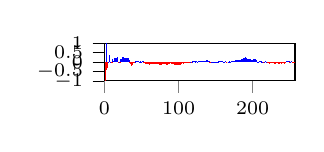
\begin{tikzpicture}

\definecolor{darkgray176}{RGB}{176,176,176}

\begin{axis}[
width=0.33\textwidth,
height=0.17\textwidth,
tick label style={font=\scriptsize},
tick align=outside,
tick pos=left,
xmin=0, xmax=257,
y grid style={darkgray176},
ymin=-1, ymax=1,
ytick style={color=black}
]
\draw[draw=none,fill=red] (axis cs:0.6,0) rectangle (axis cs:1.4,-2.93394490779936);
\draw[draw=none,fill=blue] (axis cs:1.6,0) rectangle (axis cs:2.4,1.01734823308138);
\draw[draw=none,fill=red] (axis cs:2.6,0) rectangle (axis cs:3.4,-0.398001499027313);
\draw[draw=none,fill=red] (axis cs:3.6,0) rectangle (axis cs:4.4,-0.31936145029438);
\draw[draw=none,fill=blue] (axis cs:4.6,0) rectangle (axis cs:5.4,0.00547902625882735);
\draw[draw=none,fill=blue] (axis cs:5.6,0) rectangle (axis cs:6.4,0.348104465976141);
\draw[draw=none,fill=blue] (axis cs:6.6,0) rectangle (axis cs:7.4,0.0518611248667309);
\draw[draw=none,fill=blue] (axis cs:7.6,0) rectangle (axis cs:8.4,0.00546714953477778);
\draw[draw=none,fill=red] (axis cs:8.6,0) rectangle (axis cs:9.4,-0.00862689279958939);
\draw[draw=none,fill=blue] (axis cs:9.6,0) rectangle (axis cs:10.4,0.147602154464429);
\draw[draw=none,fill=red] (axis cs:10.6,0) rectangle (axis cs:11.4,-0.0263252512816319);
\draw[draw=none,fill=blue] (axis cs:11.6,0) rectangle (axis cs:12.4,0.0505127195765267);
\draw[draw=none,fill=blue] (axis cs:12.6,0) rectangle (axis cs:13.4,0.201169113234843);
\draw[draw=none,fill=blue] (axis cs:13.6,0) rectangle (axis cs:14.4,0.212411875646231);
\draw[draw=none,fill=blue] (axis cs:14.6,0) rectangle (axis cs:15.4,0.232748287292289);
\draw[draw=none,fill=blue] (axis cs:15.6,0) rectangle (axis cs:16.4,0.213568474408738);
\draw[draw=none,fill=blue] (axis cs:16.6,0) rectangle (axis cs:17.4,0.277329403667639);
\draw[draw=none,fill=blue] (axis cs:17.6,0) rectangle (axis cs:18.4,0.226708854890127);
\draw[draw=none,fill=red] (axis cs:18.6,0) rectangle (axis cs:19.4,-0.0728291109387191);
\draw[draw=none,fill=blue] (axis cs:19.6,0) rectangle (axis cs:20.4,0.00269865656931323);
\draw[draw=none,fill=red] (axis cs:20.6,0) rectangle (axis cs:21.4,-0.0714341361262427);
\draw[draw=none,fill=blue] (axis cs:21.6,0) rectangle (axis cs:22.4,0.140489368445373);
\draw[draw=none,fill=blue] (axis cs:22.6,0) rectangle (axis cs:23.4,0.168713959542797);
\draw[draw=none,fill=blue] (axis cs:23.6,0) rectangle (axis cs:24.4,0.268989311163118);
\draw[draw=none,fill=blue] (axis cs:24.6,0) rectangle (axis cs:25.4,0.27873446203962);
\draw[draw=none,fill=blue] (axis cs:25.6,0) rectangle (axis cs:26.4,0.211821069770818);
\draw[draw=none,fill=blue] (axis cs:26.6,0) rectangle (axis cs:27.4,0.203167942146948);
\draw[draw=none,fill=blue] (axis cs:27.6,0) rectangle (axis cs:28.4,0.223727643444604);
\draw[draw=none,fill=blue] (axis cs:28.6,0) rectangle (axis cs:29.4,0.22906086616242);
\draw[draw=none,fill=blue] (axis cs:29.6,0) rectangle (axis cs:30.4,0.239323769672491);
\draw[draw=none,fill=blue] (axis cs:30.6,0) rectangle (axis cs:31.4,0.220748149968724);
\draw[draw=none,fill=blue] (axis cs:31.6,0) rectangle (axis cs:32.4,0.228599216775005);
\draw[draw=none,fill=blue] (axis cs:32.6,0) rectangle (axis cs:33.4,0.103012079872956);
\draw[draw=none,fill=red] (axis cs:33.6,0) rectangle (axis cs:34.4,-0.0485609429289786);
\draw[draw=none,fill=red] (axis cs:34.6,0) rectangle (axis cs:35.4,-0.126133190455029);
\draw[draw=none,fill=red] (axis cs:35.6,0) rectangle (axis cs:36.4,-0.187560654454047);
\draw[draw=none,fill=red] (axis cs:36.6,0) rectangle (axis cs:37.4,-0.149332574550575);
\draw[draw=none,fill=red] (axis cs:37.6,0) rectangle (axis cs:38.4,-0.0144949235479226);
\draw[draw=none,fill=red] (axis cs:38.6,0) rectangle (axis cs:39.4,-0.0139098103732502);
\draw[draw=none,fill=red] (axis cs:39.6,0) rectangle (axis cs:40.4,-0.0114522122683312);
\draw[draw=none,fill=blue] (axis cs:40.6,0) rectangle (axis cs:41.4,0.00598809424869096);
\draw[draw=none,fill=blue] (axis cs:41.6,0) rectangle (axis cs:42.4,0.0392643411886322);
\draw[draw=none,fill=blue] (axis cs:42.6,0) rectangle (axis cs:43.4,0.0279882882851918);
\draw[draw=none,fill=blue] (axis cs:43.6,0) rectangle (axis cs:44.4,0.0286687919375321);
\draw[draw=none,fill=blue] (axis cs:44.6,0) rectangle (axis cs:45.4,0.0486456570889429);
\draw[draw=none,fill=blue] (axis cs:45.6,0) rectangle (axis cs:46.4,0.0786613822276001);
\draw[draw=none,fill=blue] (axis cs:46.6,0) rectangle (axis cs:47.4,0.0212329415478818);
\draw[draw=none,fill=blue] (axis cs:47.6,0) rectangle (axis cs:48.4,0.0240608565136107);
\draw[draw=none,fill=blue] (axis cs:48.6,0) rectangle (axis cs:49.4,0.0516527265638578);
\draw[draw=none,fill=blue] (axis cs:49.6,0) rectangle (axis cs:50.4,0.0204120706945501);
\draw[draw=none,fill=blue] (axis cs:50.6,0) rectangle (axis cs:51.4,0.0631378421685449);
\draw[draw=none,fill=blue] (axis cs:51.6,0) rectangle (axis cs:52.4,0.0491697634471331);
\draw[draw=none,fill=red] (axis cs:52.6,0) rectangle (axis cs:53.4,-0.0739932207073215);
\draw[draw=none,fill=red] (axis cs:53.6,0) rectangle (axis cs:54.4,-0.0774463761180861);
\draw[draw=none,fill=red] (axis cs:54.6,0) rectangle (axis cs:55.4,-0.0957068854109941);
\draw[draw=none,fill=red] (axis cs:55.6,0) rectangle (axis cs:56.4,-0.0910010273841522);
\draw[draw=none,fill=red] (axis cs:56.6,0) rectangle (axis cs:57.4,-0.0991317584557887);
\draw[draw=none,fill=red] (axis cs:57.6,0) rectangle (axis cs:58.4,-0.11080120266215);
\draw[draw=none,fill=red] (axis cs:58.6,0) rectangle (axis cs:59.4,-0.095138159663513);
\draw[draw=none,fill=red] (axis cs:59.6,0) rectangle (axis cs:60.4,-0.129228827816713);
\draw[draw=none,fill=red] (axis cs:60.6,0) rectangle (axis cs:61.4,-0.138150917414811);
\draw[draw=none,fill=red] (axis cs:61.6,0) rectangle (axis cs:62.4,-0.123769784623743);
\draw[draw=none,fill=red] (axis cs:62.6,0) rectangle (axis cs:63.4,-0.117038954952614);
\draw[draw=none,fill=red] (axis cs:63.6,0) rectangle (axis cs:64.4,-0.0624371382782911);
\draw[draw=none,fill=red] (axis cs:64.6,0) rectangle (axis cs:65.4,-0.0982276759239831);
\draw[draw=none,fill=red] (axis cs:65.6,0) rectangle (axis cs:66.4,-0.112053921261104);
\draw[draw=none,fill=red] (axis cs:66.6,0) rectangle (axis cs:67.4,-0.118493398381594);
\draw[draw=none,fill=red] (axis cs:67.6,0) rectangle (axis cs:68.4,-0.12546042888997);
\draw[draw=none,fill=red] (axis cs:68.6,0) rectangle (axis cs:69.4,-0.10463877423706);
\draw[draw=none,fill=red] (axis cs:69.6,0) rectangle (axis cs:70.4,-0.0911809413488935);
\draw[draw=none,fill=red] (axis cs:70.6,0) rectangle (axis cs:71.4,-0.0838717266210489);
\draw[draw=none,fill=red] (axis cs:71.6,0) rectangle (axis cs:72.4,-0.109072207160028);
\draw[draw=none,fill=red] (axis cs:72.6,0) rectangle (axis cs:73.4,-0.105880527370592);
\draw[draw=none,fill=red] (axis cs:73.6,0) rectangle (axis cs:74.4,-0.157394420003785);
\draw[draw=none,fill=red] (axis cs:74.6,0) rectangle (axis cs:75.4,-0.155883461295449);
\draw[draw=none,fill=red] (axis cs:75.6,0) rectangle (axis cs:76.4,-0.157491432200023);
\draw[draw=none,fill=red] (axis cs:76.6,0) rectangle (axis cs:77.4,-0.161426240241935);
\draw[draw=none,fill=red] (axis cs:77.6,0) rectangle (axis cs:78.4,-0.106883006656717);
\draw[draw=none,fill=red] (axis cs:78.6,0) rectangle (axis cs:79.4,-0.121948133541198);
\draw[draw=none,fill=red] (axis cs:79.6,0) rectangle (axis cs:80.4,-0.121946749636876);
\draw[draw=none,fill=red] (axis cs:80.6,0) rectangle (axis cs:81.4,-0.125466604583064);
\draw[draw=none,fill=red] (axis cs:81.6,0) rectangle (axis cs:82.4,-0.123021958120822);
\draw[draw=none,fill=red] (axis cs:82.6,0) rectangle (axis cs:83.4,-0.127311696120197);
\draw[draw=none,fill=red] (axis cs:83.6,0) rectangle (axis cs:84.4,-0.152425565106278);
\draw[draw=none,fill=red] (axis cs:84.6,0) rectangle (axis cs:85.4,-0.154015999696722);
\draw[draw=none,fill=red] (axis cs:85.6,0) rectangle (axis cs:86.4,-0.106316309388612);
\draw[draw=none,fill=red] (axis cs:86.6,0) rectangle (axis cs:87.4,-0.103126213680058);
\draw[draw=none,fill=red] (axis cs:87.6,0) rectangle (axis cs:88.4,-0.0712274176788554);
\draw[draw=none,fill=red] (axis cs:88.6,0) rectangle (axis cs:89.4,-0.0734749720058776);
\draw[draw=none,fill=red] (axis cs:89.6,0) rectangle (axis cs:90.4,-0.0901574657117257);
\draw[draw=none,fill=red] (axis cs:90.6,0) rectangle (axis cs:91.4,-0.0894141261918424);
\draw[draw=none,fill=red] (axis cs:91.6,0) rectangle (axis cs:92.4,-0.0936166370462681);
\draw[draw=none,fill=red] (axis cs:92.6,0) rectangle (axis cs:93.4,-0.105422045501144);
\draw[draw=none,fill=red] (axis cs:93.6,0) rectangle (axis cs:94.4,-0.137180389306396);
\draw[draw=none,fill=red] (axis cs:94.6,0) rectangle (axis cs:95.4,-0.139597025864341);
\draw[draw=none,fill=red] (axis cs:95.6,0) rectangle (axis cs:96.4,-0.137798013040912);
\draw[draw=none,fill=red] (axis cs:96.6,0) rectangle (axis cs:97.4,-0.136262418803303);
\draw[draw=none,fill=red] (axis cs:97.6,0) rectangle (axis cs:98.4,-0.132962100379634);
\draw[draw=none,fill=red] (axis cs:98.6,0) rectangle (axis cs:99.4,-0.133780844756945);
\draw[draw=none,fill=red] (axis cs:99.6,0) rectangle (axis cs:100.4,-0.149109292976433);
\draw[draw=none,fill=red] (axis cs:100.6,0) rectangle (axis cs:101.4,-0.158262600056118);
\draw[draw=none,fill=red] (axis cs:101.6,0) rectangle (axis cs:102.4,-0.144902194117244);
\draw[draw=none,fill=red] (axis cs:102.6,0) rectangle (axis cs:103.4,-0.124129953704144);
\draw[draw=none,fill=red] (axis cs:103.6,0) rectangle (axis cs:104.4,-0.109250163018016);
\draw[draw=none,fill=red] (axis cs:104.6,0) rectangle (axis cs:105.4,-0.0718232543905688);
\draw[draw=none,fill=red] (axis cs:105.6,0) rectangle (axis cs:106.4,-0.0846583442262823);
\draw[draw=none,fill=red] (axis cs:106.6,0) rectangle (axis cs:107.4,-0.0781395409773986);
\draw[draw=none,fill=red] (axis cs:107.6,0) rectangle (axis cs:108.4,-0.074010952468726);
\draw[draw=none,fill=red] (axis cs:108.6,0) rectangle (axis cs:109.4,-0.0574078458890748);
\draw[draw=none,fill=red] (axis cs:109.6,0) rectangle (axis cs:110.4,-0.0546137613495183);
\draw[draw=none,fill=red] (axis cs:110.6,0) rectangle (axis cs:111.4,-0.035462727999799);
\draw[draw=none,fill=red] (axis cs:111.6,0) rectangle (axis cs:112.4,-0.0584180015851814);
\draw[draw=none,fill=red] (axis cs:112.6,0) rectangle (axis cs:113.4,-0.0446214623037595);
\draw[draw=none,fill=red] (axis cs:113.6,0) rectangle (axis cs:114.4,-0.0254372304213897);
\draw[draw=none,fill=red] (axis cs:114.6,0) rectangle (axis cs:115.4,-0.00901301149611422);
\draw[draw=none,fill=blue] (axis cs:115.6,0) rectangle (axis cs:116.4,0.0069771912675245);
\draw[draw=none,fill=red] (axis cs:116.6,0) rectangle (axis cs:117.4,-0.0218718894422811);
\draw[draw=none,fill=blue] (axis cs:117.6,0) rectangle (axis cs:118.4,0.00179802449327537);
\draw[draw=none,fill=blue] (axis cs:118.6,0) rectangle (axis cs:119.4,0.0315554072791562);
\draw[draw=none,fill=blue] (axis cs:119.6,0) rectangle (axis cs:120.4,0.0307430133052606);
\draw[draw=none,fill=blue] (axis cs:120.6,0) rectangle (axis cs:121.4,0.030633753239957);
\draw[draw=none,fill=blue] (axis cs:121.6,0) rectangle (axis cs:122.4,0.0412693162416358);
\draw[draw=none,fill=blue] (axis cs:122.6,0) rectangle (axis cs:123.4,0.016961095909326);
\draw[draw=none,fill=blue] (axis cs:123.6,0) rectangle (axis cs:124.4,0.0310436791619124);
\draw[draw=none,fill=blue] (axis cs:124.6,0) rectangle (axis cs:125.4,0.0230720684612966);
\draw[draw=none,fill=blue] (axis cs:125.6,0) rectangle (axis cs:126.4,0.0310456161434964);
\draw[draw=none,fill=blue] (axis cs:126.6,0) rectangle (axis cs:127.4,0.0651092813966181);
\draw[draw=none,fill=blue] (axis cs:127.6,0) rectangle (axis cs:128.4,0.0606492854324205);
\draw[draw=none,fill=blue] (axis cs:128.6,0) rectangle (axis cs:129.4,0.0615808279466403);
\draw[draw=none,fill=blue] (axis cs:129.6,0) rectangle (axis cs:130.4,0.0627544402267981);
\draw[draw=none,fill=blue] (axis cs:130.6,0) rectangle (axis cs:131.4,0.0409413436866561);
\draw[draw=none,fill=blue] (axis cs:131.6,0) rectangle (axis cs:132.4,0.0308473883068787);
\draw[draw=none,fill=blue] (axis cs:132.6,0) rectangle (axis cs:133.4,0.063100710196121);
\draw[draw=none,fill=blue] (axis cs:133.6,0) rectangle (axis cs:134.4,0.053087607208095);
\draw[draw=none,fill=blue] (axis cs:134.6,0) rectangle (axis cs:135.4,0.0570070763742012);
\draw[draw=none,fill=blue] (axis cs:135.6,0) rectangle (axis cs:136.4,0.0601927357620435);
\draw[draw=none,fill=blue] (axis cs:136.6,0) rectangle (axis cs:137.4,0.0707007480309763);
\draw[draw=none,fill=blue] (axis cs:137.6,0) rectangle (axis cs:138.4,0.102877769051626);
\draw[draw=none,fill=blue] (axis cs:138.6,0) rectangle (axis cs:139.4,0.106178641197197);
\draw[draw=none,fill=blue] (axis cs:139.6,0) rectangle (axis cs:140.4,0.0597352245443306);
\draw[draw=none,fill=blue] (axis cs:140.6,0) rectangle (axis cs:141.4,0.0366231237767307);
\draw[draw=none,fill=red] (axis cs:141.6,0) rectangle (axis cs:142.4,-0.0247200345496994);
\draw[draw=none,fill=red] (axis cs:142.6,0) rectangle (axis cs:143.4,-0.00341446515307409);
\draw[draw=none,fill=blue] (axis cs:143.6,0) rectangle (axis cs:144.4,0.00509309508931199);
\draw[draw=none,fill=red] (axis cs:144.6,0) rectangle (axis cs:145.4,-0.00112122389988345);
\draw[draw=none,fill=blue] (axis cs:145.6,0) rectangle (axis cs:146.4,0.0132444719546925);
\draw[draw=none,fill=blue] (axis cs:146.6,0) rectangle (axis cs:147.4,0.0107087982276814);
\draw[draw=none,fill=blue] (axis cs:147.6,0) rectangle (axis cs:148.4,0.00199308707582002);
\draw[draw=none,fill=blue] (axis cs:148.6,0) rectangle (axis cs:149.4,0.0205065658329904);
\draw[draw=none,fill=blue] (axis cs:149.6,0) rectangle (axis cs:150.4,0.0183159395483754);
\draw[draw=none,fill=blue] (axis cs:150.6,0) rectangle (axis cs:151.4,0.0169884063266119);
\draw[draw=none,fill=blue] (axis cs:151.6,0) rectangle (axis cs:152.4,0.0165485597079318);
\draw[draw=none,fill=blue] (axis cs:152.6,0) rectangle (axis cs:153.4,0.0218519836257909);
\draw[draw=none,fill=blue] (axis cs:153.6,0) rectangle (axis cs:154.4,0.0355417553673445);
\draw[draw=none,fill=blue] (axis cs:154.6,0) rectangle (axis cs:155.4,0.0473596809631784);
\draw[draw=none,fill=blue] (axis cs:155.6,0) rectangle (axis cs:156.4,0.0615669100589473);
\draw[draw=none,fill=blue] (axis cs:156.6,0) rectangle (axis cs:157.4,0.0433525383660425);
\draw[draw=none,fill=blue] (axis cs:157.6,0) rectangle (axis cs:158.4,0.0583221710444577);
\draw[draw=none,fill=blue] (axis cs:158.6,0) rectangle (axis cs:159.4,0.037945851014539);
\draw[draw=none,fill=blue] (axis cs:159.6,0) rectangle (axis cs:160.4,0.00994286789249488);
\draw[draw=none,fill=blue] (axis cs:160.6,0) rectangle (axis cs:161.4,0.019166300906639);
\draw[draw=none,fill=blue] (axis cs:161.6,0) rectangle (axis cs:162.4,0.0269259128563961);
\draw[draw=none,fill=blue] (axis cs:162.6,0) rectangle (axis cs:163.4,0.048433563713425);
\draw[draw=none,fill=blue] (axis cs:163.6,0) rectangle (axis cs:164.4,0.00397326601183146);
\draw[draw=none,fill=red] (axis cs:164.6,0) rectangle (axis cs:165.4,-0.00718383551082802);
\draw[draw=none,fill=blue] (axis cs:165.6,0) rectangle (axis cs:166.4,0.000509687758921906);
\draw[draw=none,fill=blue] (axis cs:166.6,0) rectangle (axis cs:167.4,0.0124877392350311);
\draw[draw=none,fill=blue] (axis cs:167.6,0) rectangle (axis cs:168.4,0.0271412885132958);
\draw[draw=none,fill=blue] (axis cs:168.6,0) rectangle (axis cs:169.4,0.0593485080703715);
\draw[draw=none,fill=blue] (axis cs:169.6,0) rectangle (axis cs:170.4,0.014320220136828);
\draw[draw=none,fill=blue] (axis cs:170.6,0) rectangle (axis cs:171.4,0.0483515301437518);
\draw[draw=none,fill=blue] (axis cs:171.6,0) rectangle (axis cs:172.4,0.0778242976335548);
\draw[draw=none,fill=blue] (axis cs:172.6,0) rectangle (axis cs:173.4,0.0477767070557951);
\draw[draw=none,fill=blue] (axis cs:173.6,0) rectangle (axis cs:174.4,0.062924573950832);
\draw[draw=none,fill=blue] (axis cs:174.6,0) rectangle (axis cs:175.4,0.0663346779918328);
\draw[draw=none,fill=blue] (axis cs:175.6,0) rectangle (axis cs:176.4,0.0834222037666343);
\draw[draw=none,fill=blue] (axis cs:176.6,0) rectangle (axis cs:177.4,0.101946659509073);
\draw[draw=none,fill=blue] (axis cs:177.6,0) rectangle (axis cs:178.4,0.0948720623587489);
\draw[draw=none,fill=blue] (axis cs:178.6,0) rectangle (axis cs:179.4,0.0990076226305501);
\draw[draw=none,fill=blue] (axis cs:179.6,0) rectangle (axis cs:180.4,0.100546201576754);
\draw[draw=none,fill=blue] (axis cs:180.6,0) rectangle (axis cs:181.4,0.0944963738891653);
\draw[draw=none,fill=blue] (axis cs:181.6,0) rectangle (axis cs:182.4,0.125384070310274);
\draw[draw=none,fill=blue] (axis cs:182.6,0) rectangle (axis cs:183.4,0.120246095827885);
\draw[draw=none,fill=blue] (axis cs:183.6,0) rectangle (axis cs:184.4,0.146172563543815);
\draw[draw=none,fill=blue] (axis cs:184.6,0) rectangle (axis cs:185.4,0.15214901723471);
\draw[draw=none,fill=blue] (axis cs:185.6,0) rectangle (axis cs:186.4,0.164008557587132);
\draw[draw=none,fill=blue] (axis cs:186.6,0) rectangle (axis cs:187.4,0.214705891958816);
\draw[draw=none,fill=blue] (axis cs:187.6,0) rectangle (axis cs:188.4,0.229546036386856);
\draw[draw=none,fill=blue] (axis cs:188.6,0) rectangle (axis cs:189.4,0.229329205734213);
\draw[draw=none,fill=blue] (axis cs:189.6,0) rectangle (axis cs:190.4,0.240215576611547);
\draw[draw=none,fill=blue] (axis cs:190.6,0) rectangle (axis cs:191.4,0.193310353674653);
\draw[draw=none,fill=blue] (axis cs:191.6,0) rectangle (axis cs:192.4,0.189105635181582);
\draw[draw=none,fill=blue] (axis cs:192.6,0) rectangle (axis cs:193.4,0.183547785803634);
\draw[draw=none,fill=blue] (axis cs:193.6,0) rectangle (axis cs:194.4,0.17812325521875);
\draw[draw=none,fill=blue] (axis cs:194.6,0) rectangle (axis cs:195.4,0.161720223915694);
\draw[draw=none,fill=blue] (axis cs:195.6,0) rectangle (axis cs:196.4,0.140160333638603);
\draw[draw=none,fill=blue] (axis cs:196.6,0) rectangle (axis cs:197.4,0.134189027784962);
\draw[draw=none,fill=blue] (axis cs:197.6,0) rectangle (axis cs:198.4,0.123942142670163);
\draw[draw=none,fill=blue] (axis cs:198.6,0) rectangle (axis cs:199.4,0.10300524004664);
\draw[draw=none,fill=blue] (axis cs:199.6,0) rectangle (axis cs:200.4,0.116783090538891);
\draw[draw=none,fill=blue] (axis cs:200.6,0) rectangle (axis cs:201.4,0.149871220704446);
\draw[draw=none,fill=blue] (axis cs:201.6,0) rectangle (axis cs:202.4,0.145663972707855);
\draw[draw=none,fill=blue] (axis cs:202.6,0) rectangle (axis cs:203.4,0.164209488064607);
\draw[draw=none,fill=blue] (axis cs:203.6,0) rectangle (axis cs:204.4,0.118197177090447);
\draw[draw=none,fill=blue] (axis cs:204.6,0) rectangle (axis cs:205.4,0.101426623819031);
\draw[draw=none,fill=blue] (axis cs:205.6,0) rectangle (axis cs:206.4,0.00947546503265961);
\draw[draw=none,fill=blue] (axis cs:206.6,0) rectangle (axis cs:207.4,0.0132201471551685);
\draw[draw=none,fill=blue] (axis cs:207.6,0) rectangle (axis cs:208.4,0.0263188431252668);
\draw[draw=none,fill=blue] (axis cs:208.6,0) rectangle (axis cs:209.4,0.0314631558450174);
\draw[draw=none,fill=blue] (axis cs:209.6,0) rectangle (axis cs:210.4,0.033199555478054);
\draw[draw=none,fill=blue] (axis cs:210.6,0) rectangle (axis cs:211.4,0.0394243824438201);
\draw[draw=none,fill=blue] (axis cs:211.6,0) rectangle (axis cs:212.4,0.0231987337936421);
\draw[draw=none,fill=blue] (axis cs:212.6,0) rectangle (axis cs:213.4,0.0130639240499648);
\draw[draw=none,fill=red] (axis cs:213.6,0) rectangle (axis cs:214.4,-0.0248773135239317);
\draw[draw=none,fill=red] (axis cs:214.6,0) rectangle (axis cs:215.4,-0.00291354080590533);
\draw[draw=none,fill=blue] (axis cs:215.6,0) rectangle (axis cs:216.4,0.0205600642998047);
\draw[draw=none,fill=blue] (axis cs:216.6,0) rectangle (axis cs:217.4,0.0335295639910087);
\draw[draw=none,fill=red] (axis cs:217.6,0) rectangle (axis cs:218.4,-0.000954916372970072);
\draw[draw=none,fill=blue] (axis cs:218.6,0) rectangle (axis cs:219.4,0.00193567116665916);
\draw[draw=none,fill=red] (axis cs:219.6,0) rectangle (axis cs:220.4,-0.0412531702108128);
\draw[draw=none,fill=red] (axis cs:220.6,0) rectangle (axis cs:221.4,-0.0491088686133647);
\draw[draw=none,fill=red] (axis cs:221.6,0) rectangle (axis cs:222.4,-0.0807635462938929);
\draw[draw=none,fill=red] (axis cs:222.6,0) rectangle (axis cs:223.4,-0.0625078458474038);
\draw[draw=none,fill=red] (axis cs:223.6,0) rectangle (axis cs:224.4,-0.0596014423139284);
\draw[draw=none,fill=red] (axis cs:224.6,0) rectangle (axis cs:225.4,-0.0578753804325753);
\draw[draw=none,fill=red] (axis cs:225.6,0) rectangle (axis cs:226.4,-0.0564975540914281);
\draw[draw=none,fill=red] (axis cs:226.6,0) rectangle (axis cs:227.4,-0.0690468556193538);
\draw[draw=none,fill=red] (axis cs:227.6,0) rectangle (axis cs:228.4,-0.0605359438072548);
\draw[draw=none,fill=red] (axis cs:228.6,0) rectangle (axis cs:229.4,-0.0853695263870948);
\draw[draw=none,fill=red] (axis cs:229.6,0) rectangle (axis cs:230.4,-0.0908650888516509);
\draw[draw=none,fill=red] (axis cs:230.6,0) rectangle (axis cs:231.4,-0.0522290848301044);
\draw[draw=none,fill=red] (axis cs:231.6,0) rectangle (axis cs:232.4,-0.0548248866153269);
\draw[draw=none,fill=red] (axis cs:232.6,0) rectangle (axis cs:233.4,-0.0443605243034897);
\draw[draw=none,fill=red] (axis cs:233.6,0) rectangle (axis cs:234.4,-0.12151797180602);
\draw[draw=none,fill=red] (axis cs:234.6,0) rectangle (axis cs:235.4,-0.099279386072221);
\draw[draw=none,fill=red] (axis cs:235.6,0) rectangle (axis cs:236.4,-0.090299068490004);
\draw[draw=none,fill=red] (axis cs:236.6,0) rectangle (axis cs:237.4,-0.070882254013751);
\draw[draw=none,fill=red] (axis cs:237.6,0) rectangle (axis cs:238.4,-0.121818438583445);
\draw[draw=none,fill=red] (axis cs:238.6,0) rectangle (axis cs:239.4,-0.110676430561555);
\draw[draw=none,fill=red] (axis cs:239.6,0) rectangle (axis cs:240.4,-0.0571959364934405);
\draw[draw=none,fill=red] (axis cs:240.6,0) rectangle (axis cs:241.4,-0.0455570758713004);
\draw[draw=none,fill=red] (axis cs:241.6,0) rectangle (axis cs:242.4,-0.0751456538298814);
\draw[draw=none,fill=red] (axis cs:242.6,0) rectangle (axis cs:243.4,-0.0780150712206005);
\draw[draw=none,fill=red] (axis cs:243.6,0) rectangle (axis cs:244.4,-0.027021652329567);
\draw[draw=none,fill=blue] (axis cs:244.6,0) rectangle (axis cs:245.4,0.0448146099988496);
\draw[draw=none,fill=blue] (axis cs:245.6,0) rectangle (axis cs:246.4,0.0615524900881526);
\draw[draw=none,fill=blue] (axis cs:246.6,0) rectangle (axis cs:247.4,0.0612030941786812);
\draw[draw=none,fill=blue] (axis cs:247.6,0) rectangle (axis cs:248.4,0.0624017734771365);
\draw[draw=none,fill=blue] (axis cs:248.6,0) rectangle (axis cs:249.4,0.0460953312346959);
\draw[draw=none,fill=red] (axis cs:249.6,0) rectangle (axis cs:250.4,-0.0667057364935202);
\draw[draw=none,fill=blue] (axis cs:250.6,0) rectangle (axis cs:251.4,0.00427181185077674);
\draw[draw=none,fill=blue] (axis cs:251.6,0) rectangle (axis cs:252.4,0.0402149230730957);
\draw[draw=none,fill=blue] (axis cs:252.6,0) rectangle (axis cs:253.4,0.00627177690434122);
\draw[draw=none,fill=red] (axis cs:253.6,0) rectangle (axis cs:254.4,-0.00986207758891244);
\draw[draw=none,fill=red] (axis cs:254.6,0) rectangle (axis cs:255.4,-0.0467787291908228);
\draw[draw=none,fill=red] (axis cs:255.6,0) rectangle (axis cs:256.4,-0.0389300709849667);
\end{axis}

\end{tikzpicture}

        \caption{SHAP values of DMAD}
        \label{fig:shap_dmad}
    \end{subfigure}
    \label{fig:shap}
    \caption{\textbf{SHAP values of stage 1 (left), stage 2 (middle), and the difference (right).} Each bar represents the SHAP values of a single feature with respect to different classes. The object query consists of 256 features, forming 256 bars in each chart. The difference is computed as stage 1 minus stage 2, aggregating all classes, where \textcolor{red}{red} indicates a negative value and \textcolor{blue}{blue} signifies a positive value.}
\end{figure*}

\textbf{Open-loop planning.} 
We adopt the evaluation method of VAD~\cite{jiang2023vad}, which accommodates the widest range of models to our knowledge.
We report our results in \cref{tab:planning}. 
Notably, jointly optimizing $L_2$ distances and collision rates proves challenging. While PARA-Drive achieves the lowest $L_2$ distances, it also exhibits the highest collision rates.
We validate that the improvements in perception can be propagated to planning, achieving SOTA collision rates.
Note that the planning module of UniAD explicitly uses perception results to avoid collision, thereby deriving greater benefits from improved perception compared to SparseDrive.





\subsection{Ablation Study}
We ablate our proposed decoders, as shown in \cref{tab:ablation_dmad}, decomposing the motion decoder into three components: motion query, inter-layer, and inter-frame reference point updating. \\

\textbf{Model profile.} In methods with multi-view camera images as inputs, the primary computational cost is concentrated in the image backbone \cite{li2022bevformer}. In contrast, our approach focuses on the decoding component, resulting in minimal impact on model size and inference speed. Compared to UniAD~\cite{hu2023planning}, our decoders add 5.4M parameters and increase inference latency by 0.02 seconds on an \mbox{NVIDIA RTX 6000 Ada.}\\

\textbf{Effect of dividing and merging.} Experiments ID 1, 2, 3, 7 demonstrate the effectiveness of both proposed decoders. The standalone application of the interactive semantic decoder (ID 2) significantly enhances the performance of object detection, tracking, and map segmentation. The standalone application of the Neural-Bayes motion decoder (ID 3) markedly improves prediction and planning. Notably, ID 3 also significantly enhances detection and tracking, attributed to freeing object queries from learning velocities and the higher-quality reference points provided by the unimodal prediction. Experiments ID 4, 5, 6, 7 show the importance of inter-layer and inter-frame updating in the Neural-Bayes motion decoder. An incomplete Neural-Bayes motion decoder (ID 4, 5, 6) degrades detection and tracking results. Only combining both updates enables the model to achieve optimal performance.

\subsection{Visualizations}

We use SHAP values~\cite{NIPS2017_7062} to inspect the negative transfer in detection and tracking.
SHAP values quantify the contribution of each feature to the change in a model's output. %
We visualize the SHAP values of the object query with respect to the object classification output. Changes in SHAP values across the two training stages reveal the negative transfer in UniAD and highlight the effectiveness of our method.


\Cref{fig:shap_uniad} compares the SHAP values between stage 1 and stage 2 of UniAD, sorted in descending order. The left half of the difference bar chart predominantly shows negative values, whereas the right half shows positive values. This indicates that SHAP values in stage 1 are more uniformly distributed, while those in stage 2 are more concentrated. Compared with a flat distribution, this concentration indicates that fewer features are contributing to the classification task, reducing detection and tracking performance.
This observation aligns with our argument that during the second stage, object queries are expected to learn motion information, which does not benefit the perception task. 
Specifically, while the velocity learned in stage 1 is sufficient for tracking (predicting the next timestep), it is inadequate for the long-term prediction over 12 timesteps (6 seconds). 
Therefore, the object query is forced to learn more motion states that offer limited utility for identifying objects, interfering with the space for semantic information. 
In contrast, the SHAP values in DMAD maintain a similar distribution across both stages, as shown in \cref{fig:shap_dmad}.

Beyond SHAP values, we provide qualitative comparisons between DMAD and UniAD in the supplementary material \cref{app:vis}.
